\subsection*{—}
\noindent
\begin{minipage}[t]{0.49\textwidth}\centering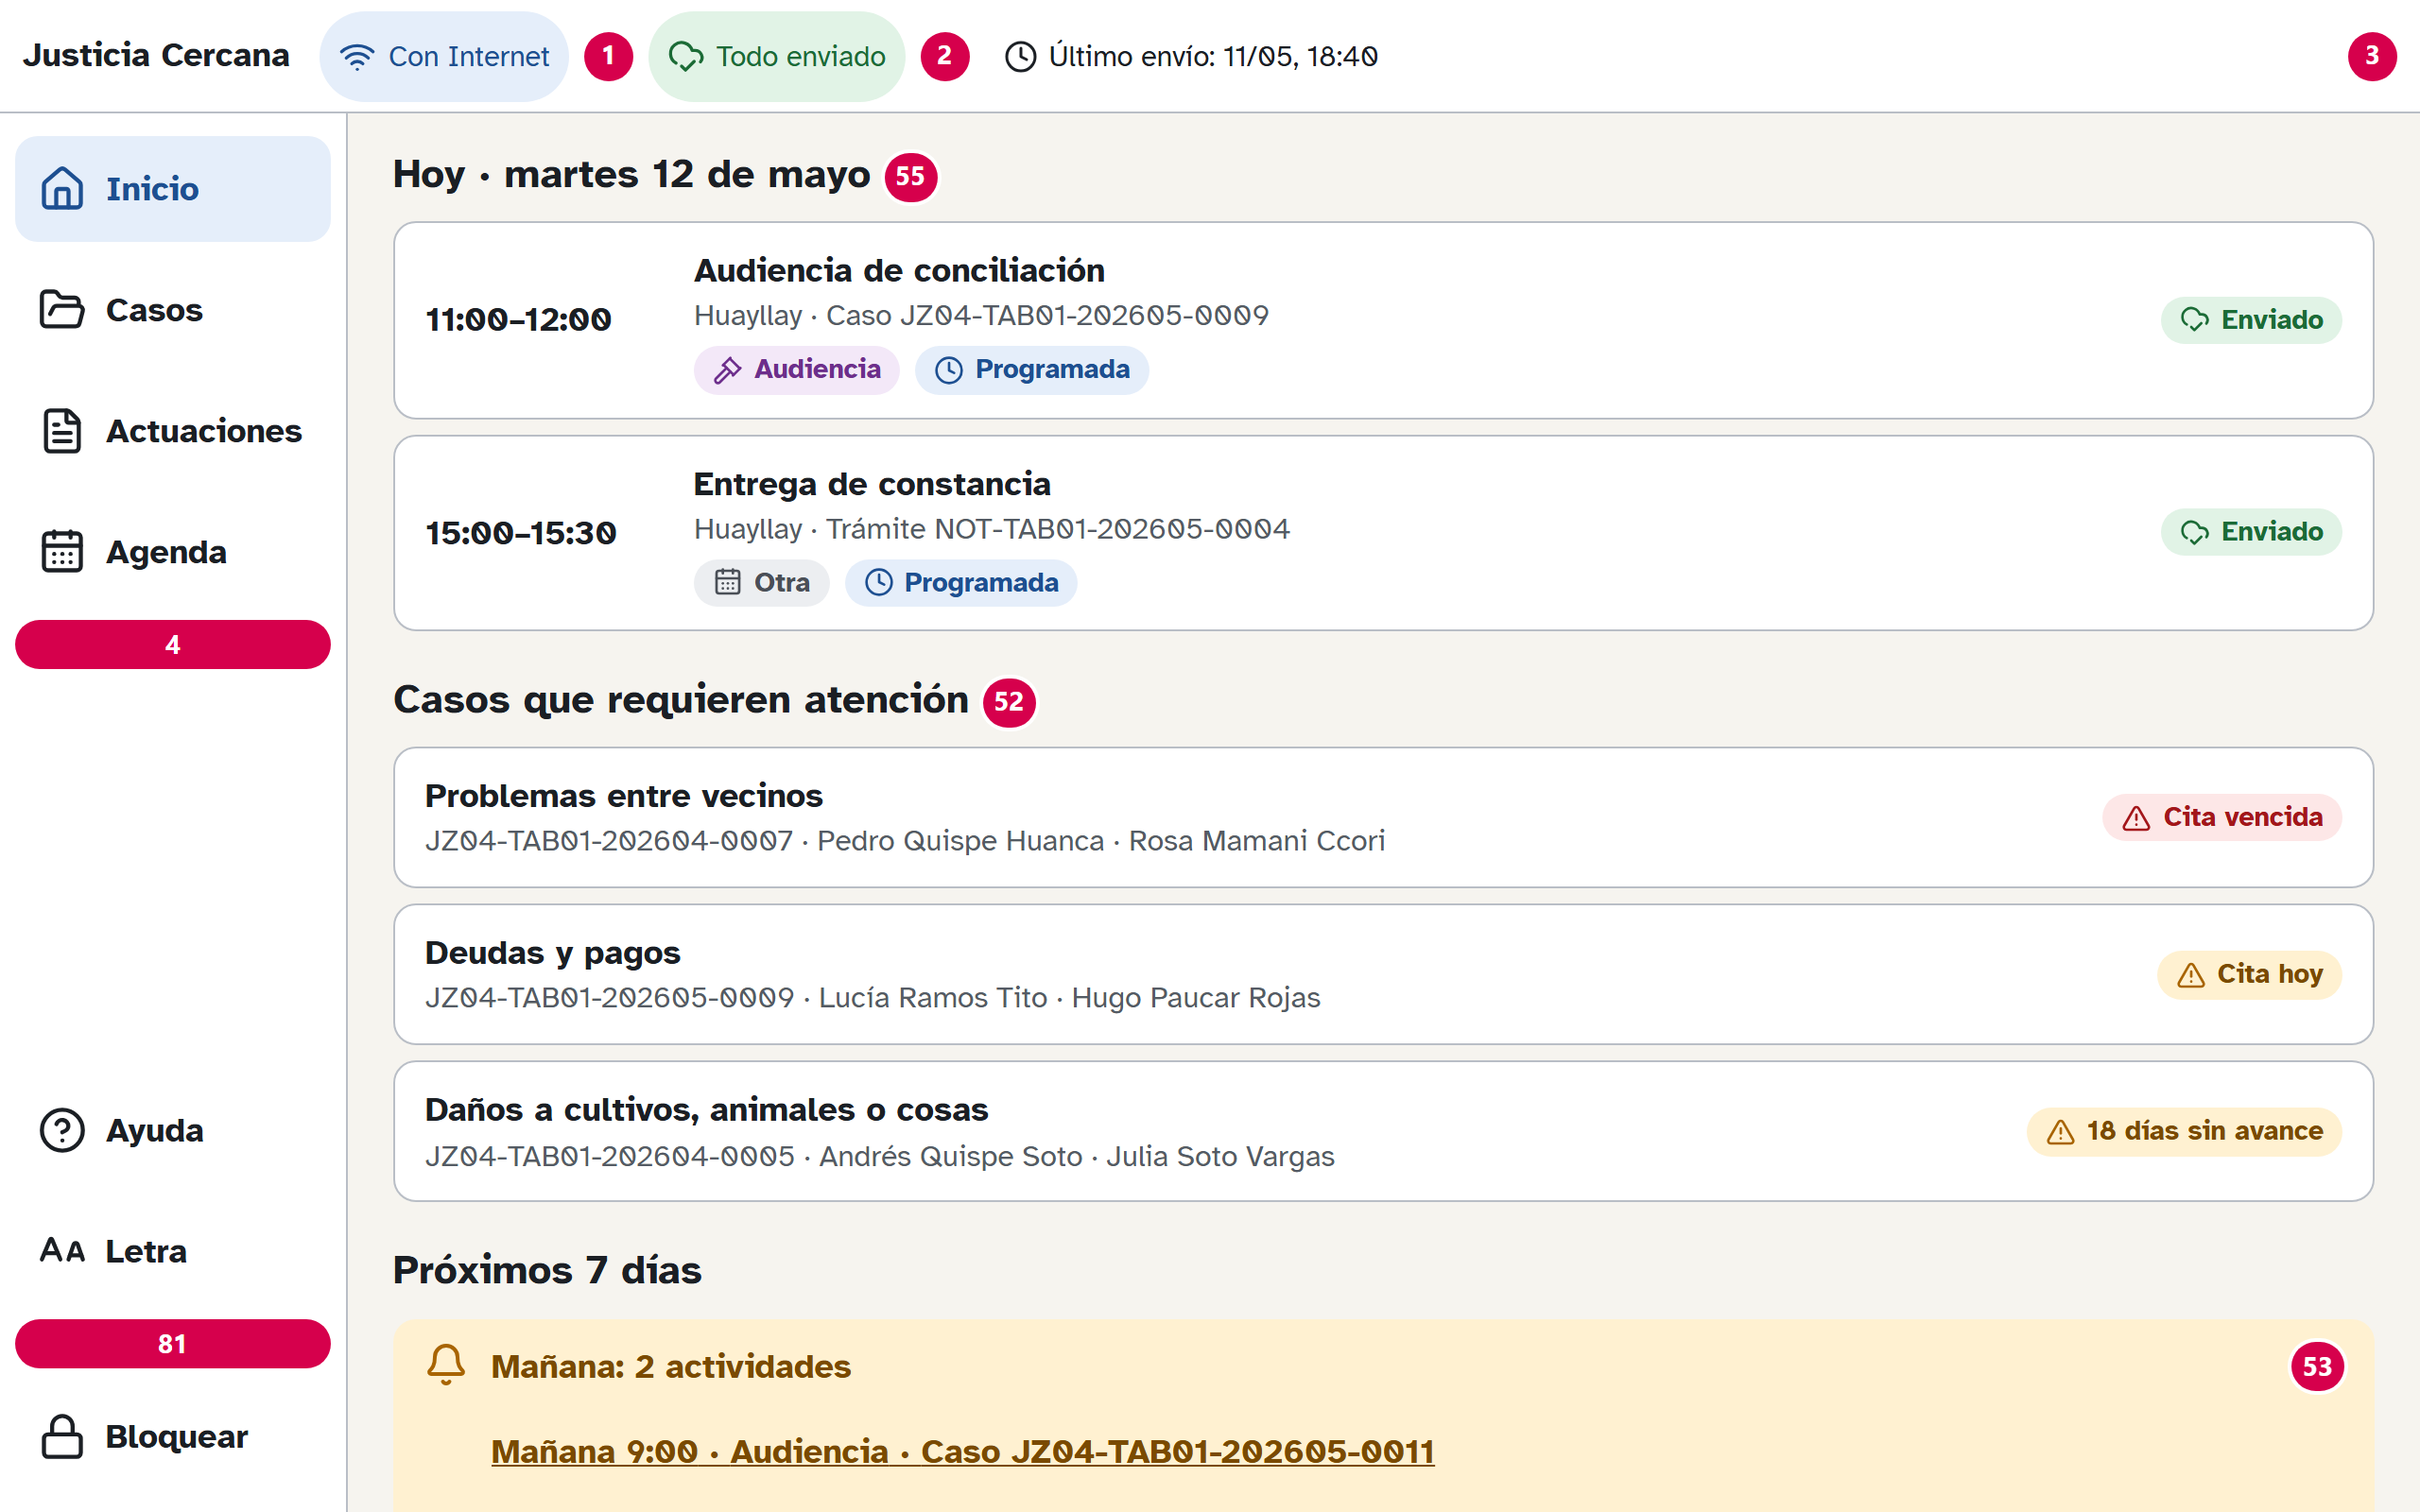
\includegraphics[width=\linewidth]{../../captures/ANOT_P-01_inicio.png}\\[-2pt]{\footnotesize\raggedright\textbf{P-01.} Marcadores numerados = IDs de la matriz de justificación \emph{(Justificación de las decisiones)}\par}\end{minipage}\hfill
\begin{minipage}[t]{0.49\textwidth}\centering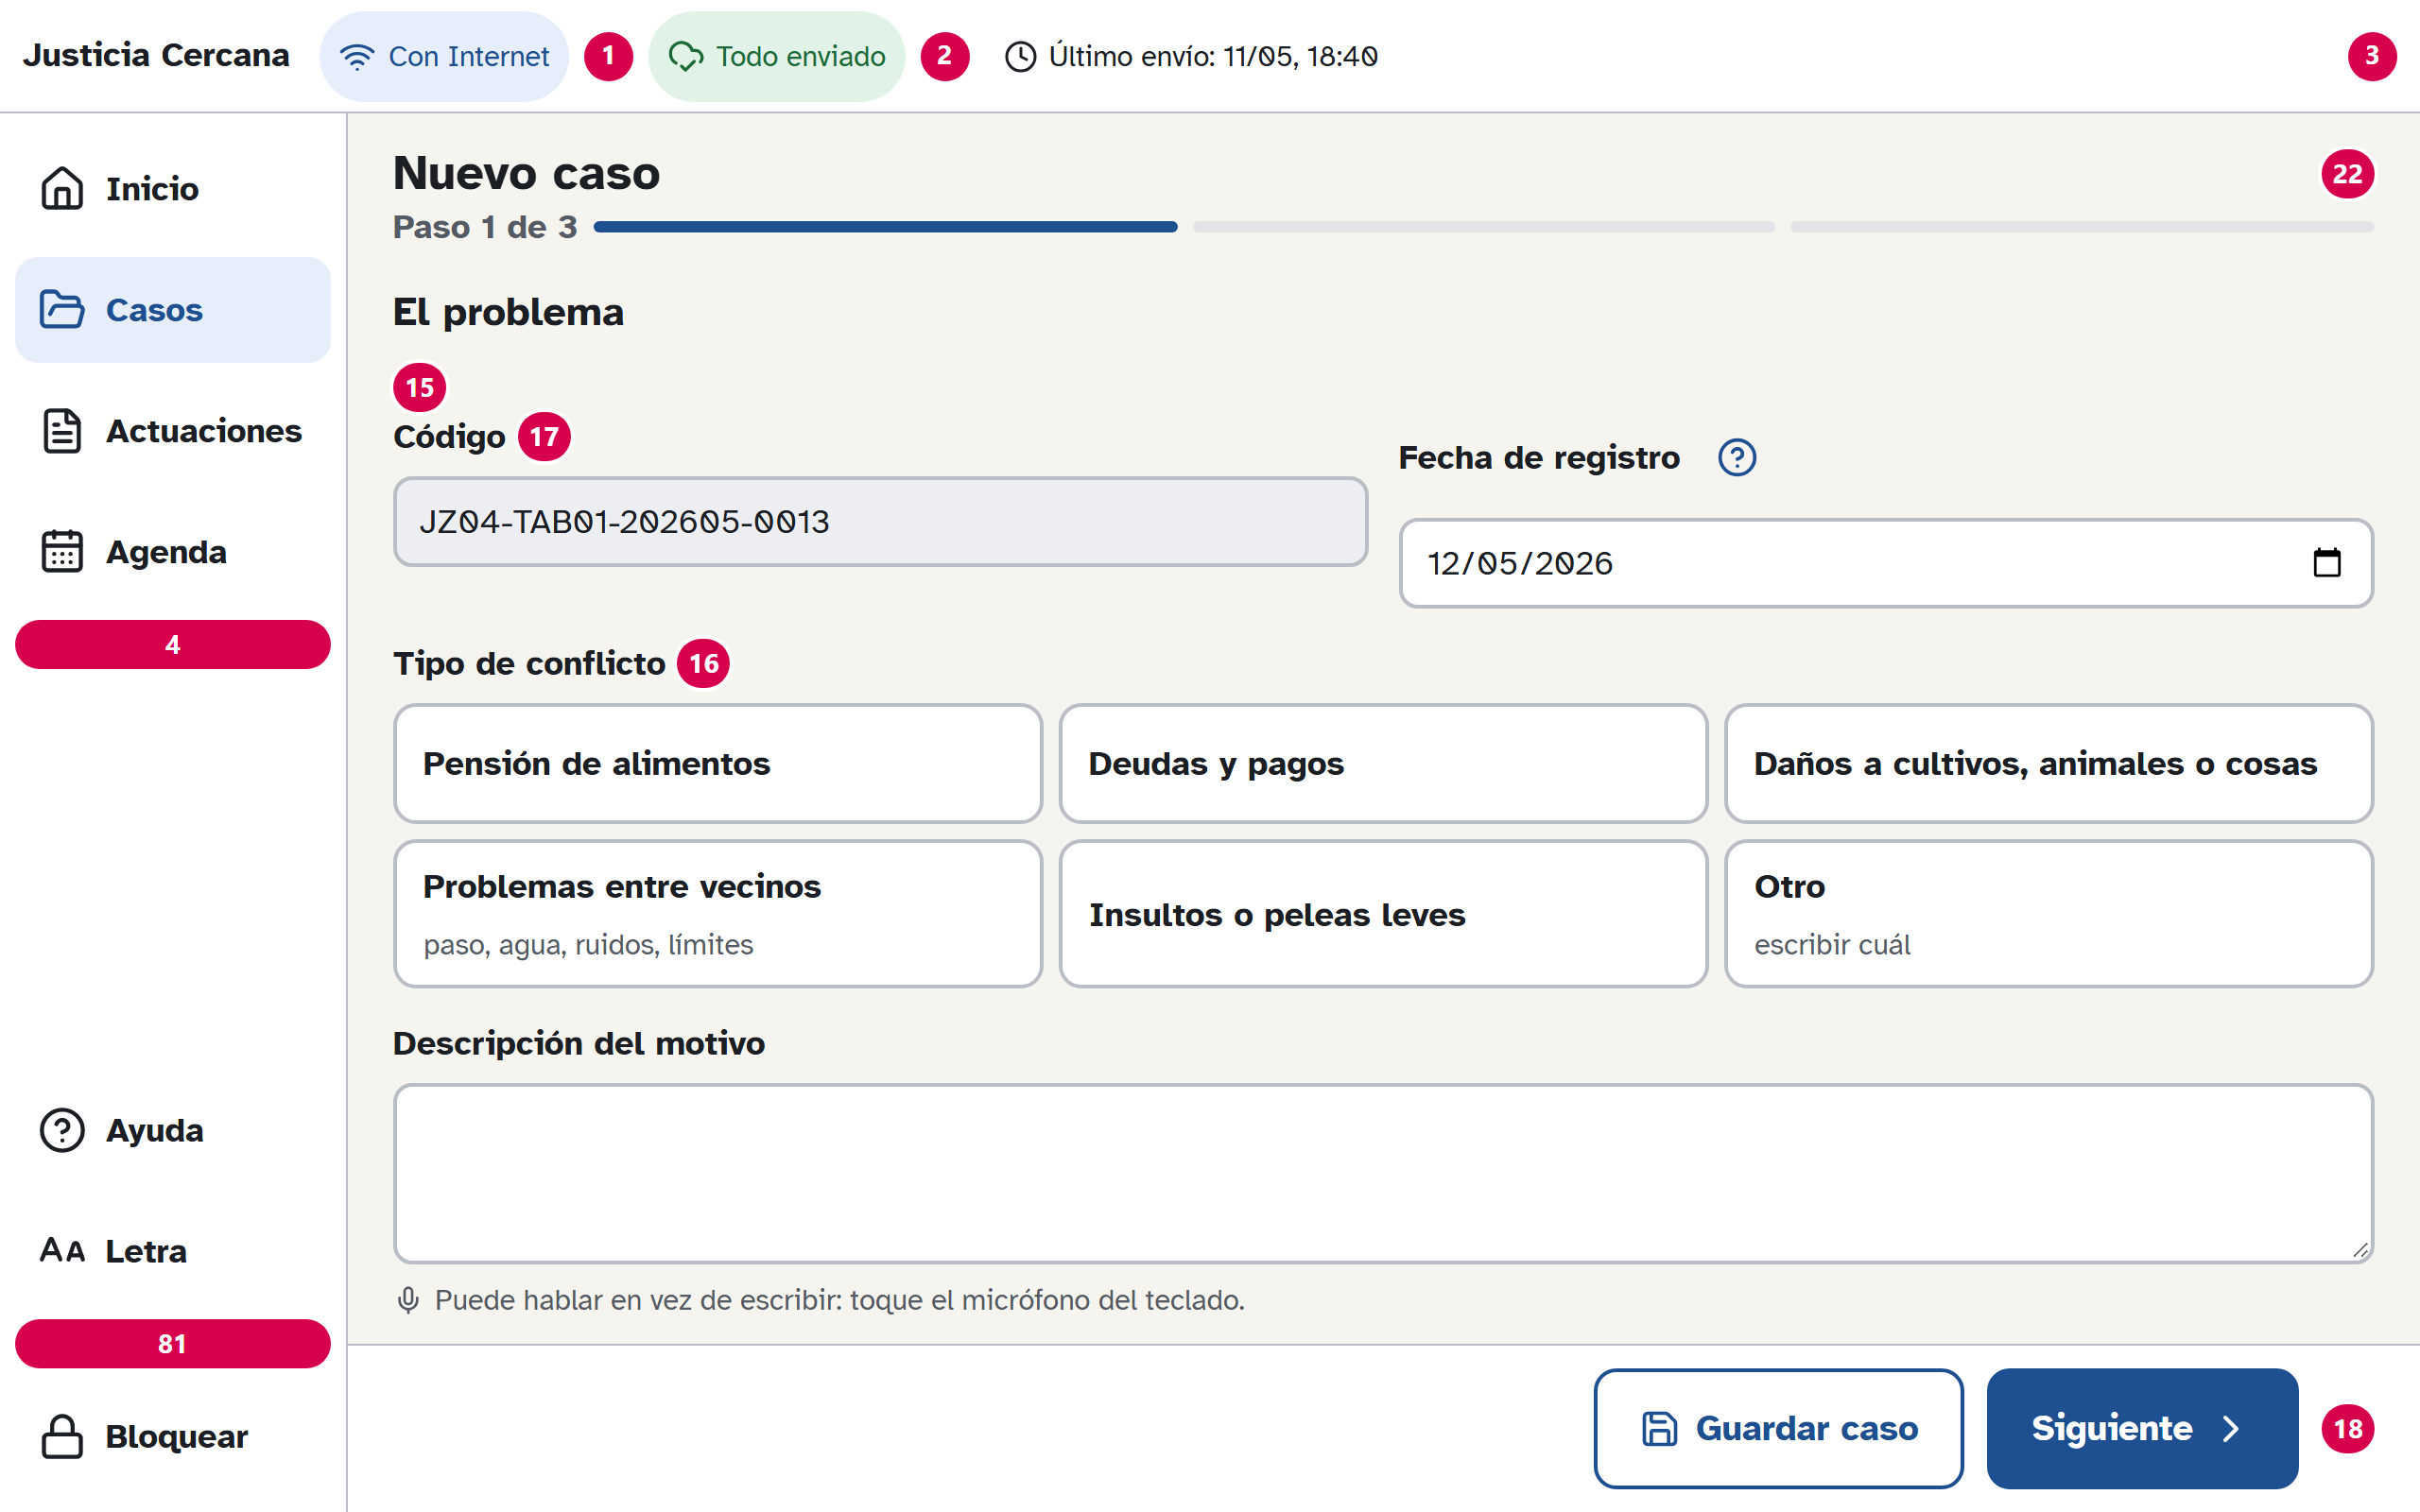
\includegraphics[width=\linewidth]{../../captures/ANOT_P-03_caso-nuevo.png}\\[-2pt]{\footnotesize\raggedright\textbf{P-03.} Marcadores numerados = IDs de la matriz de justificación \emph{(Justificación de las decisiones)}\par}\end{minipage}\par\vspace{8pt}\noindent
\begin{minipage}[t]{0.49\textwidth}\centering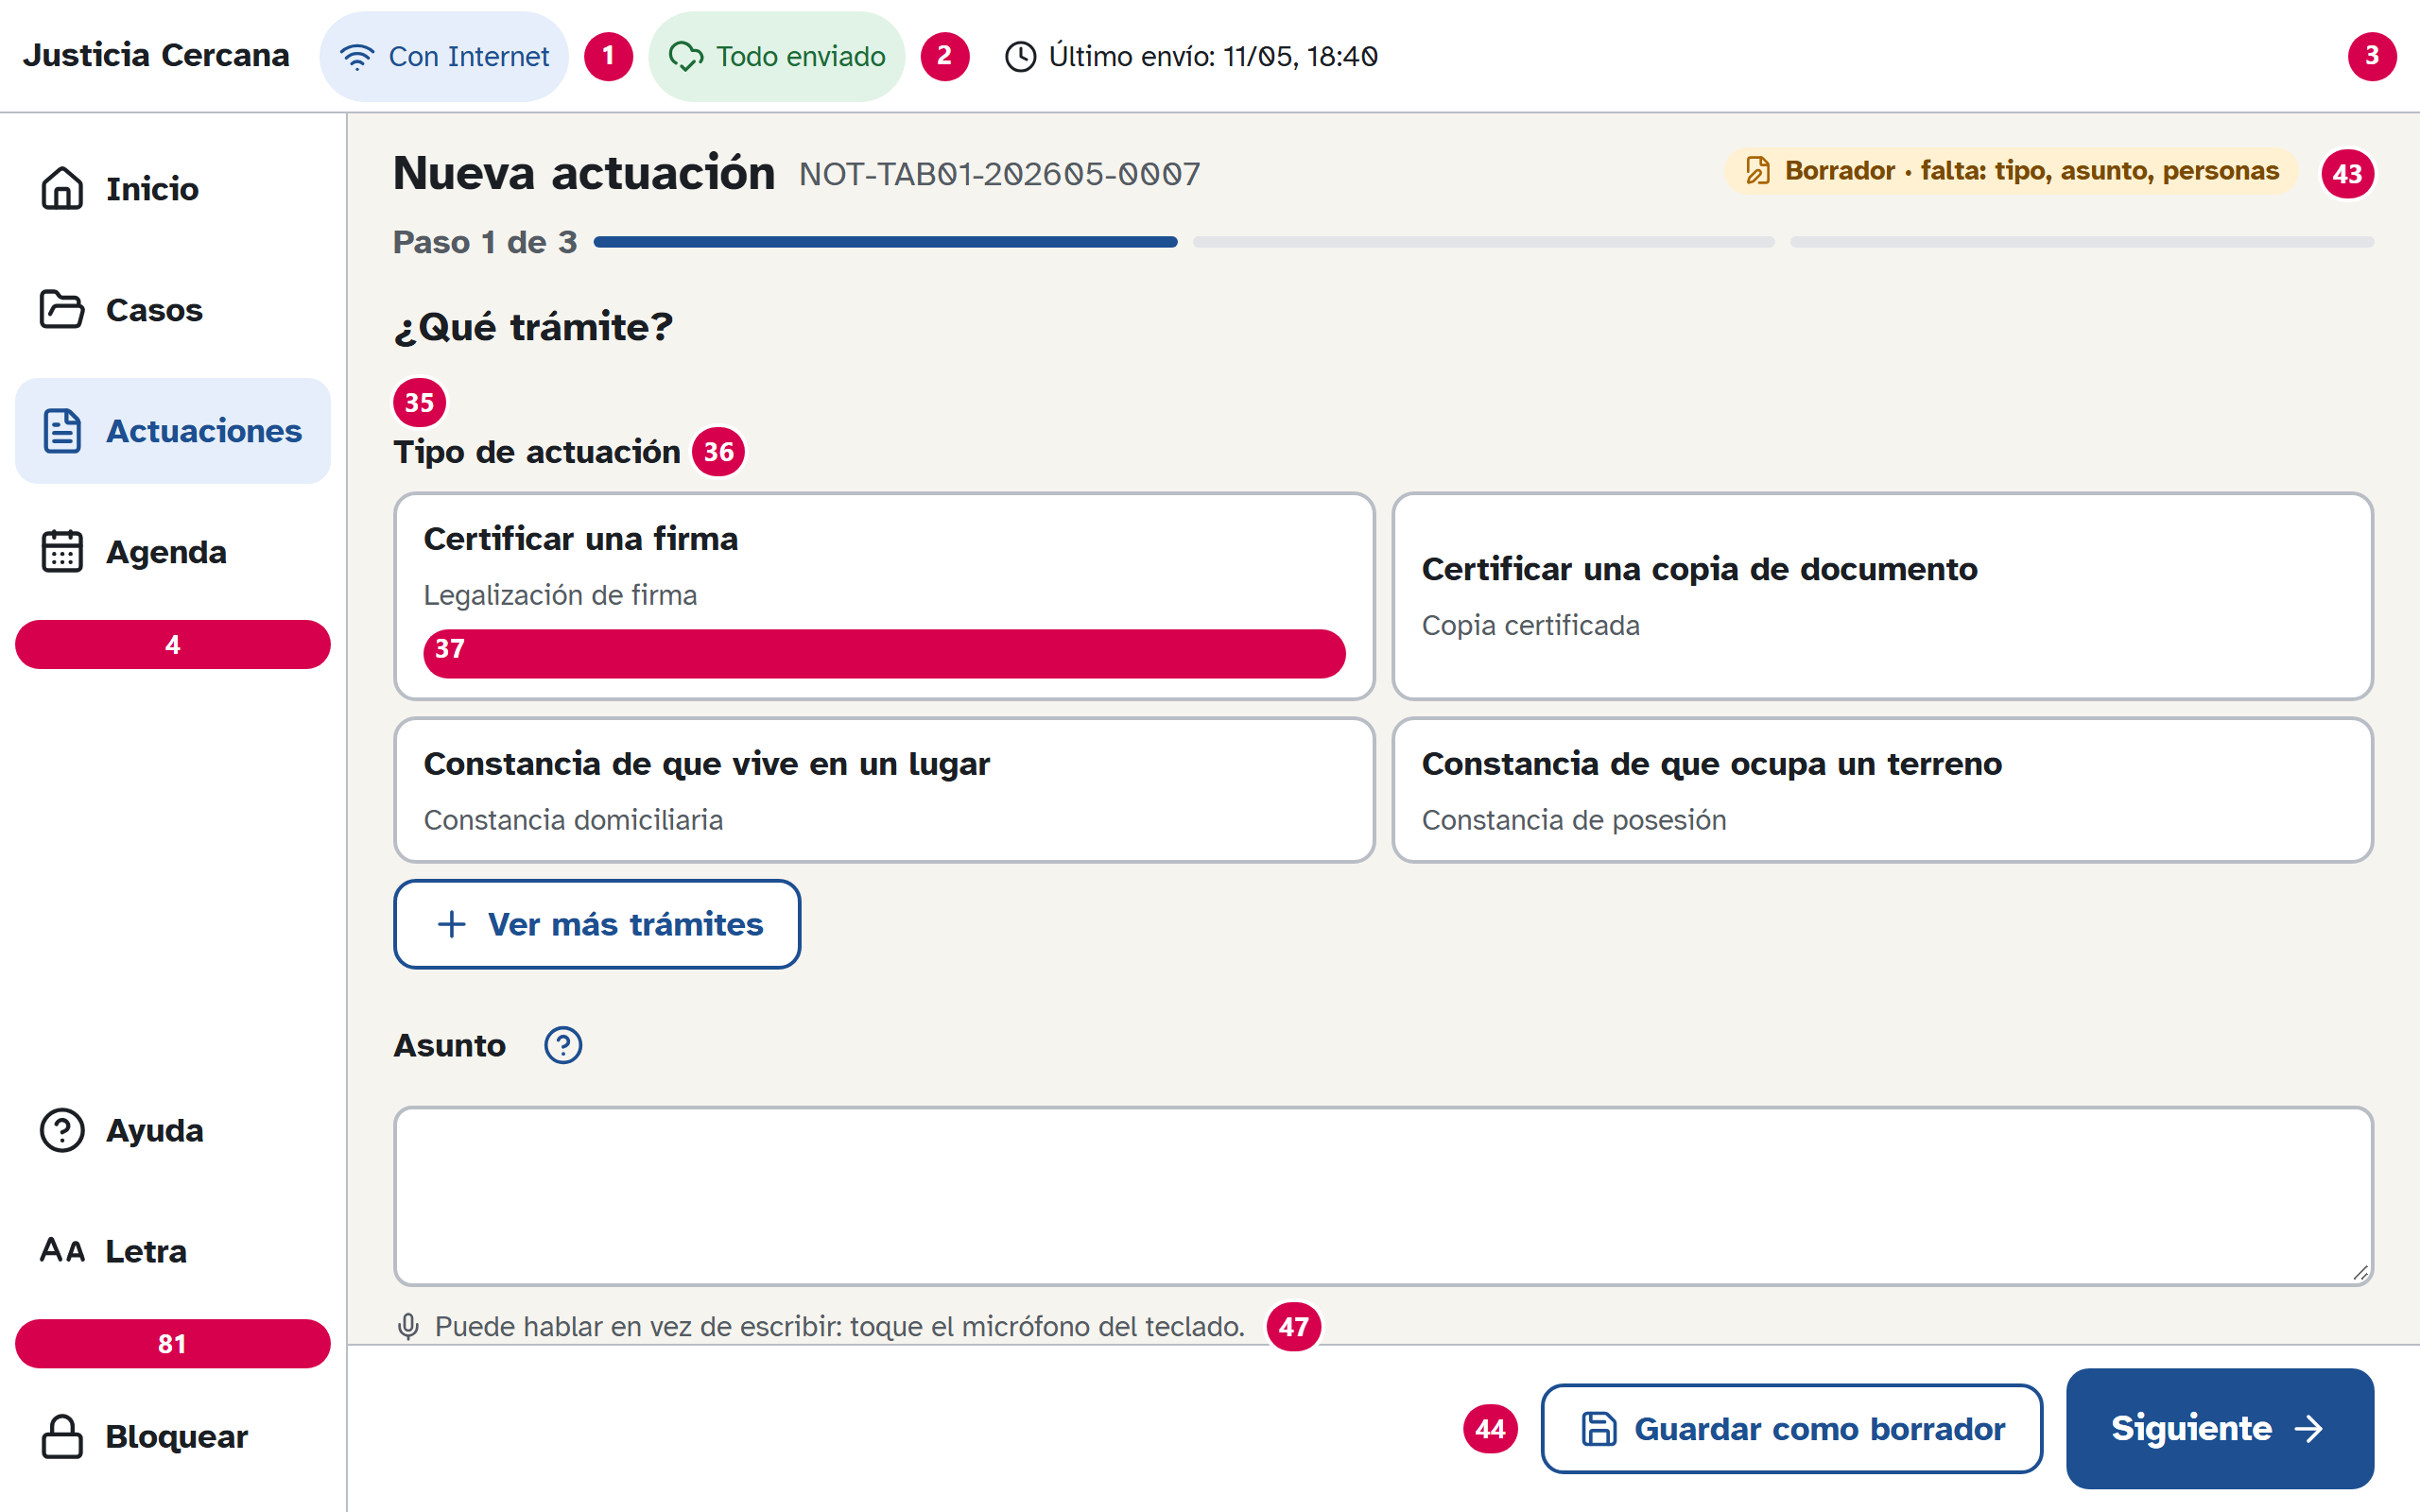
\includegraphics[width=\linewidth]{../../captures/ANOT_P-06_actuacion-nueva.png}\\[-2pt]{\footnotesize\raggedright\textbf{P-06.} Marcadores numerados = IDs de la matriz de justificación \emph{(Justificación de las decisiones)}\par}\end{minipage}\hfill
\begin{minipage}[t]{0.49\textwidth}\centering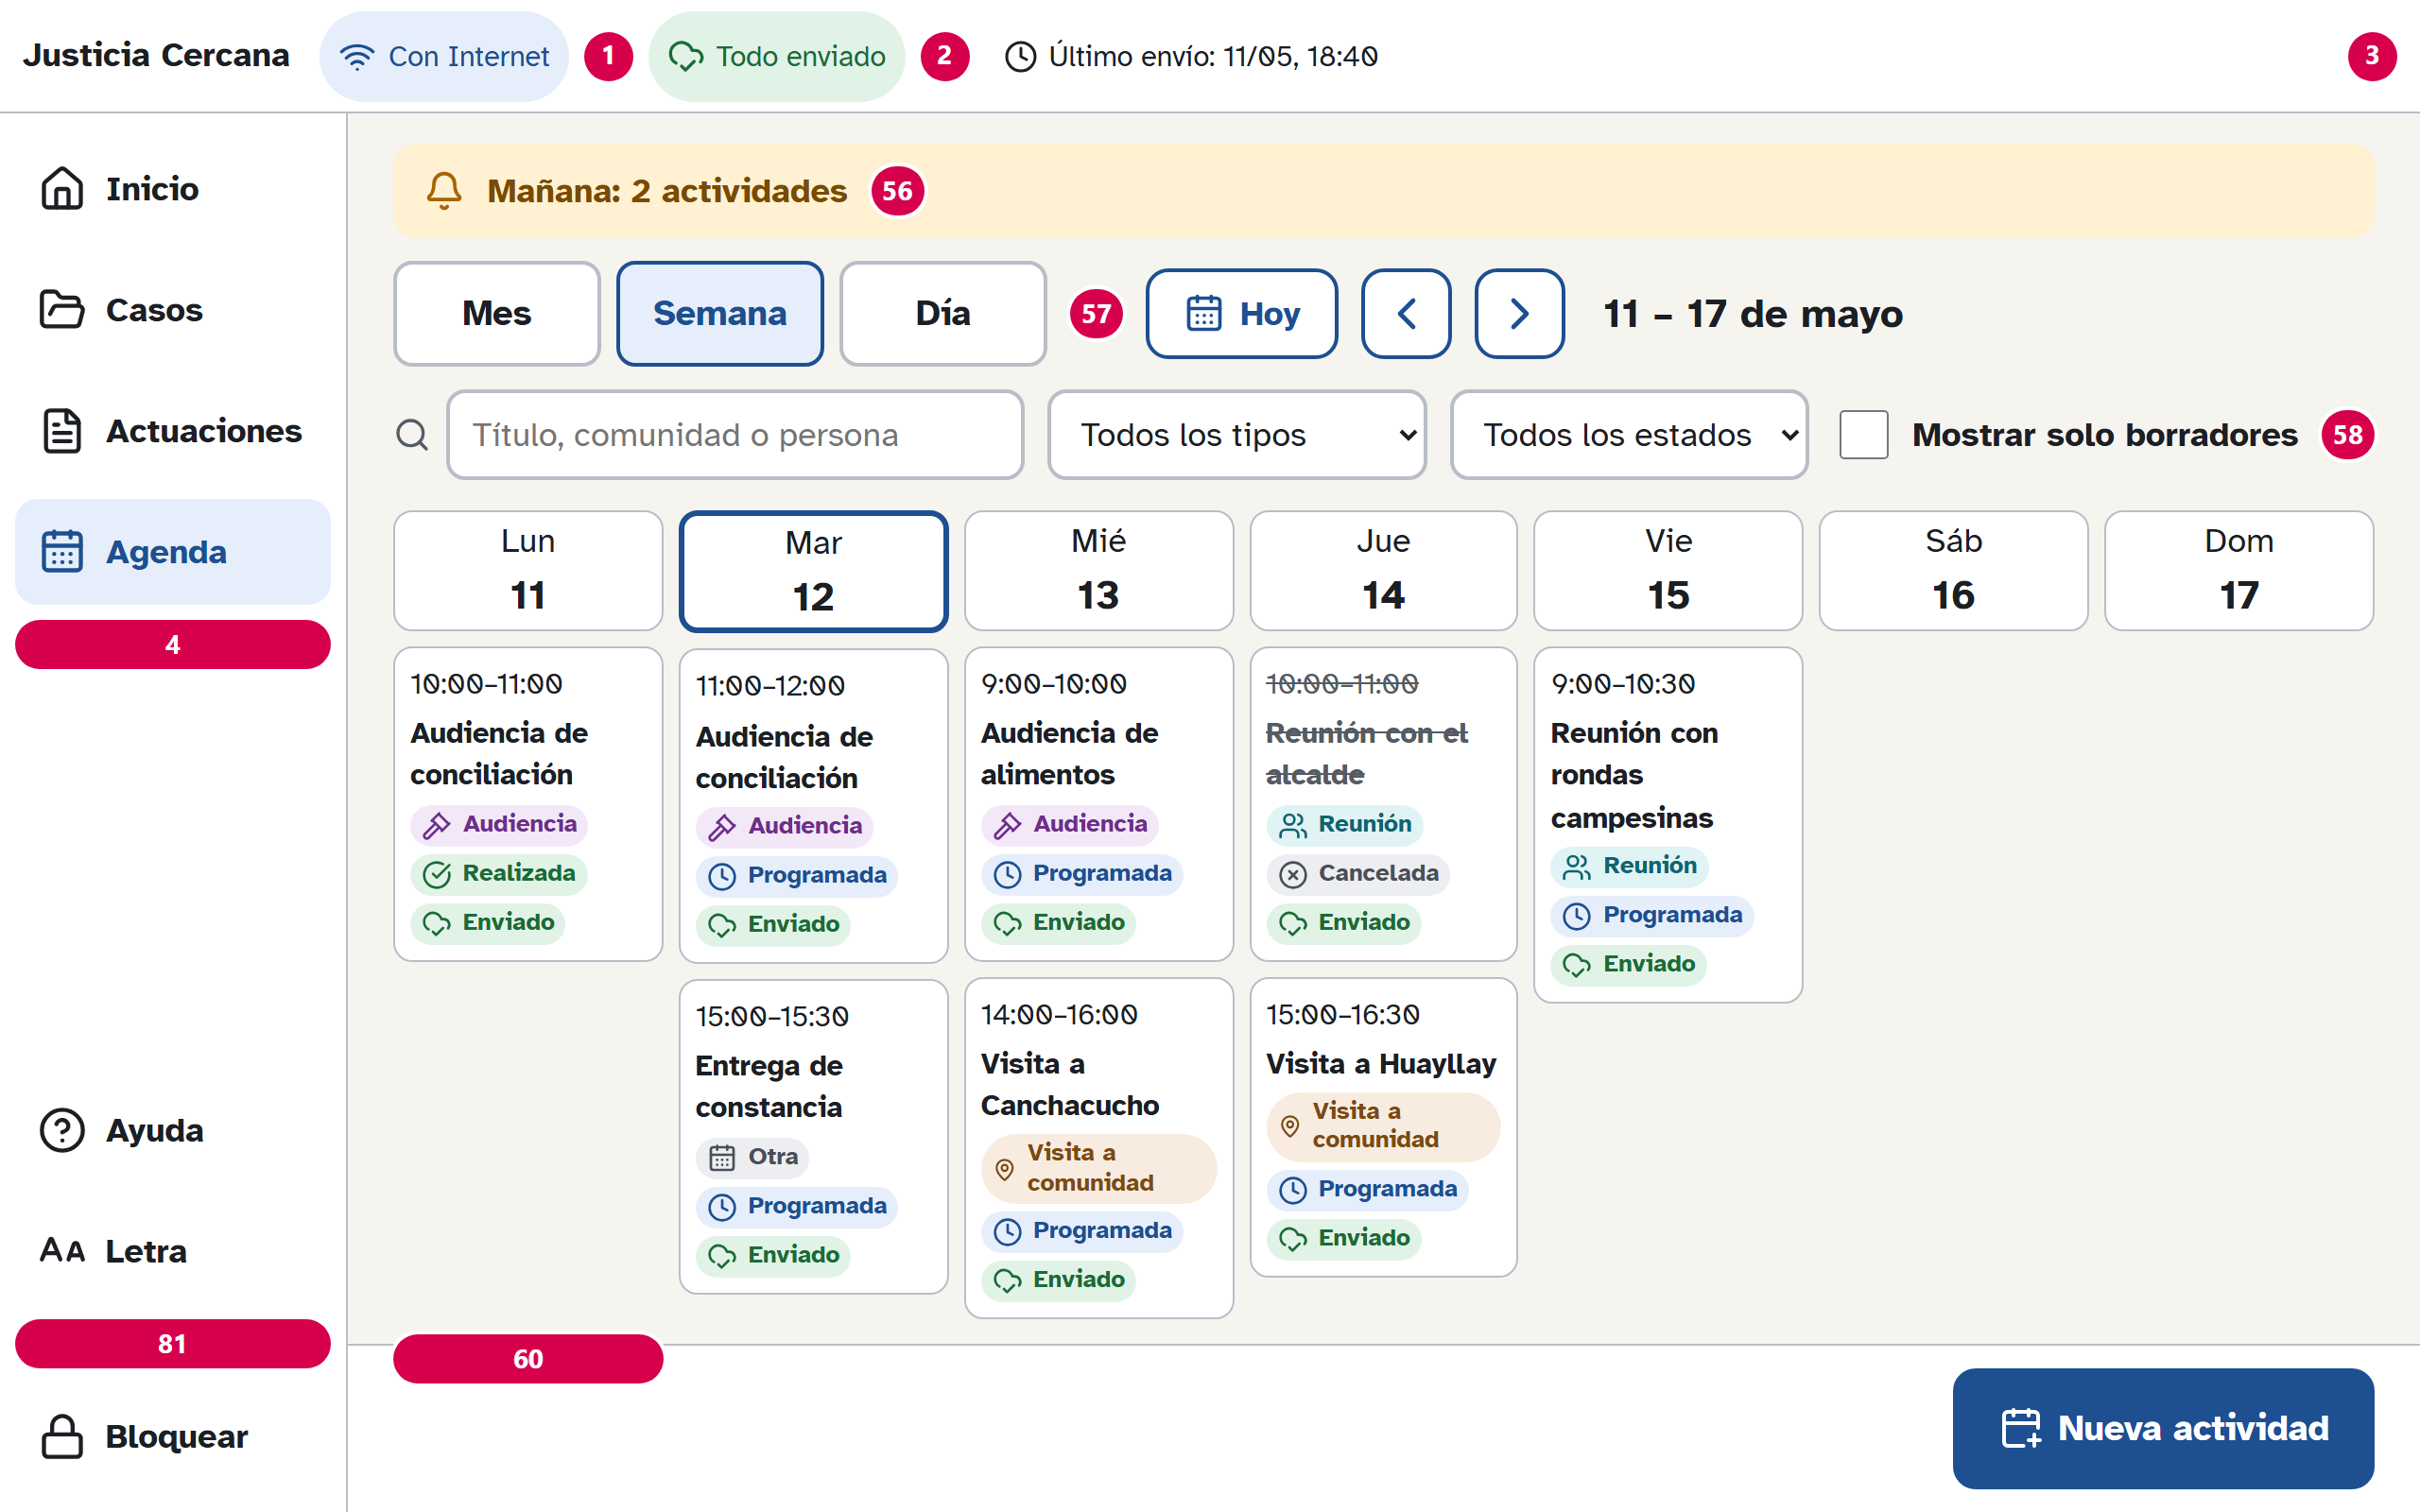
\includegraphics[width=\linewidth]{../../captures/ANOT_P-07_agenda.png}\\[-2pt]{\footnotesize\raggedright\textbf{P-07.} Marcadores numerados = IDs de la matriz de justificación \emph{(Justificación de las decisiones)}\par}\end{minipage}\par\vspace{8pt}\noindent
\begin{minipage}[t]{0.49\textwidth}\centering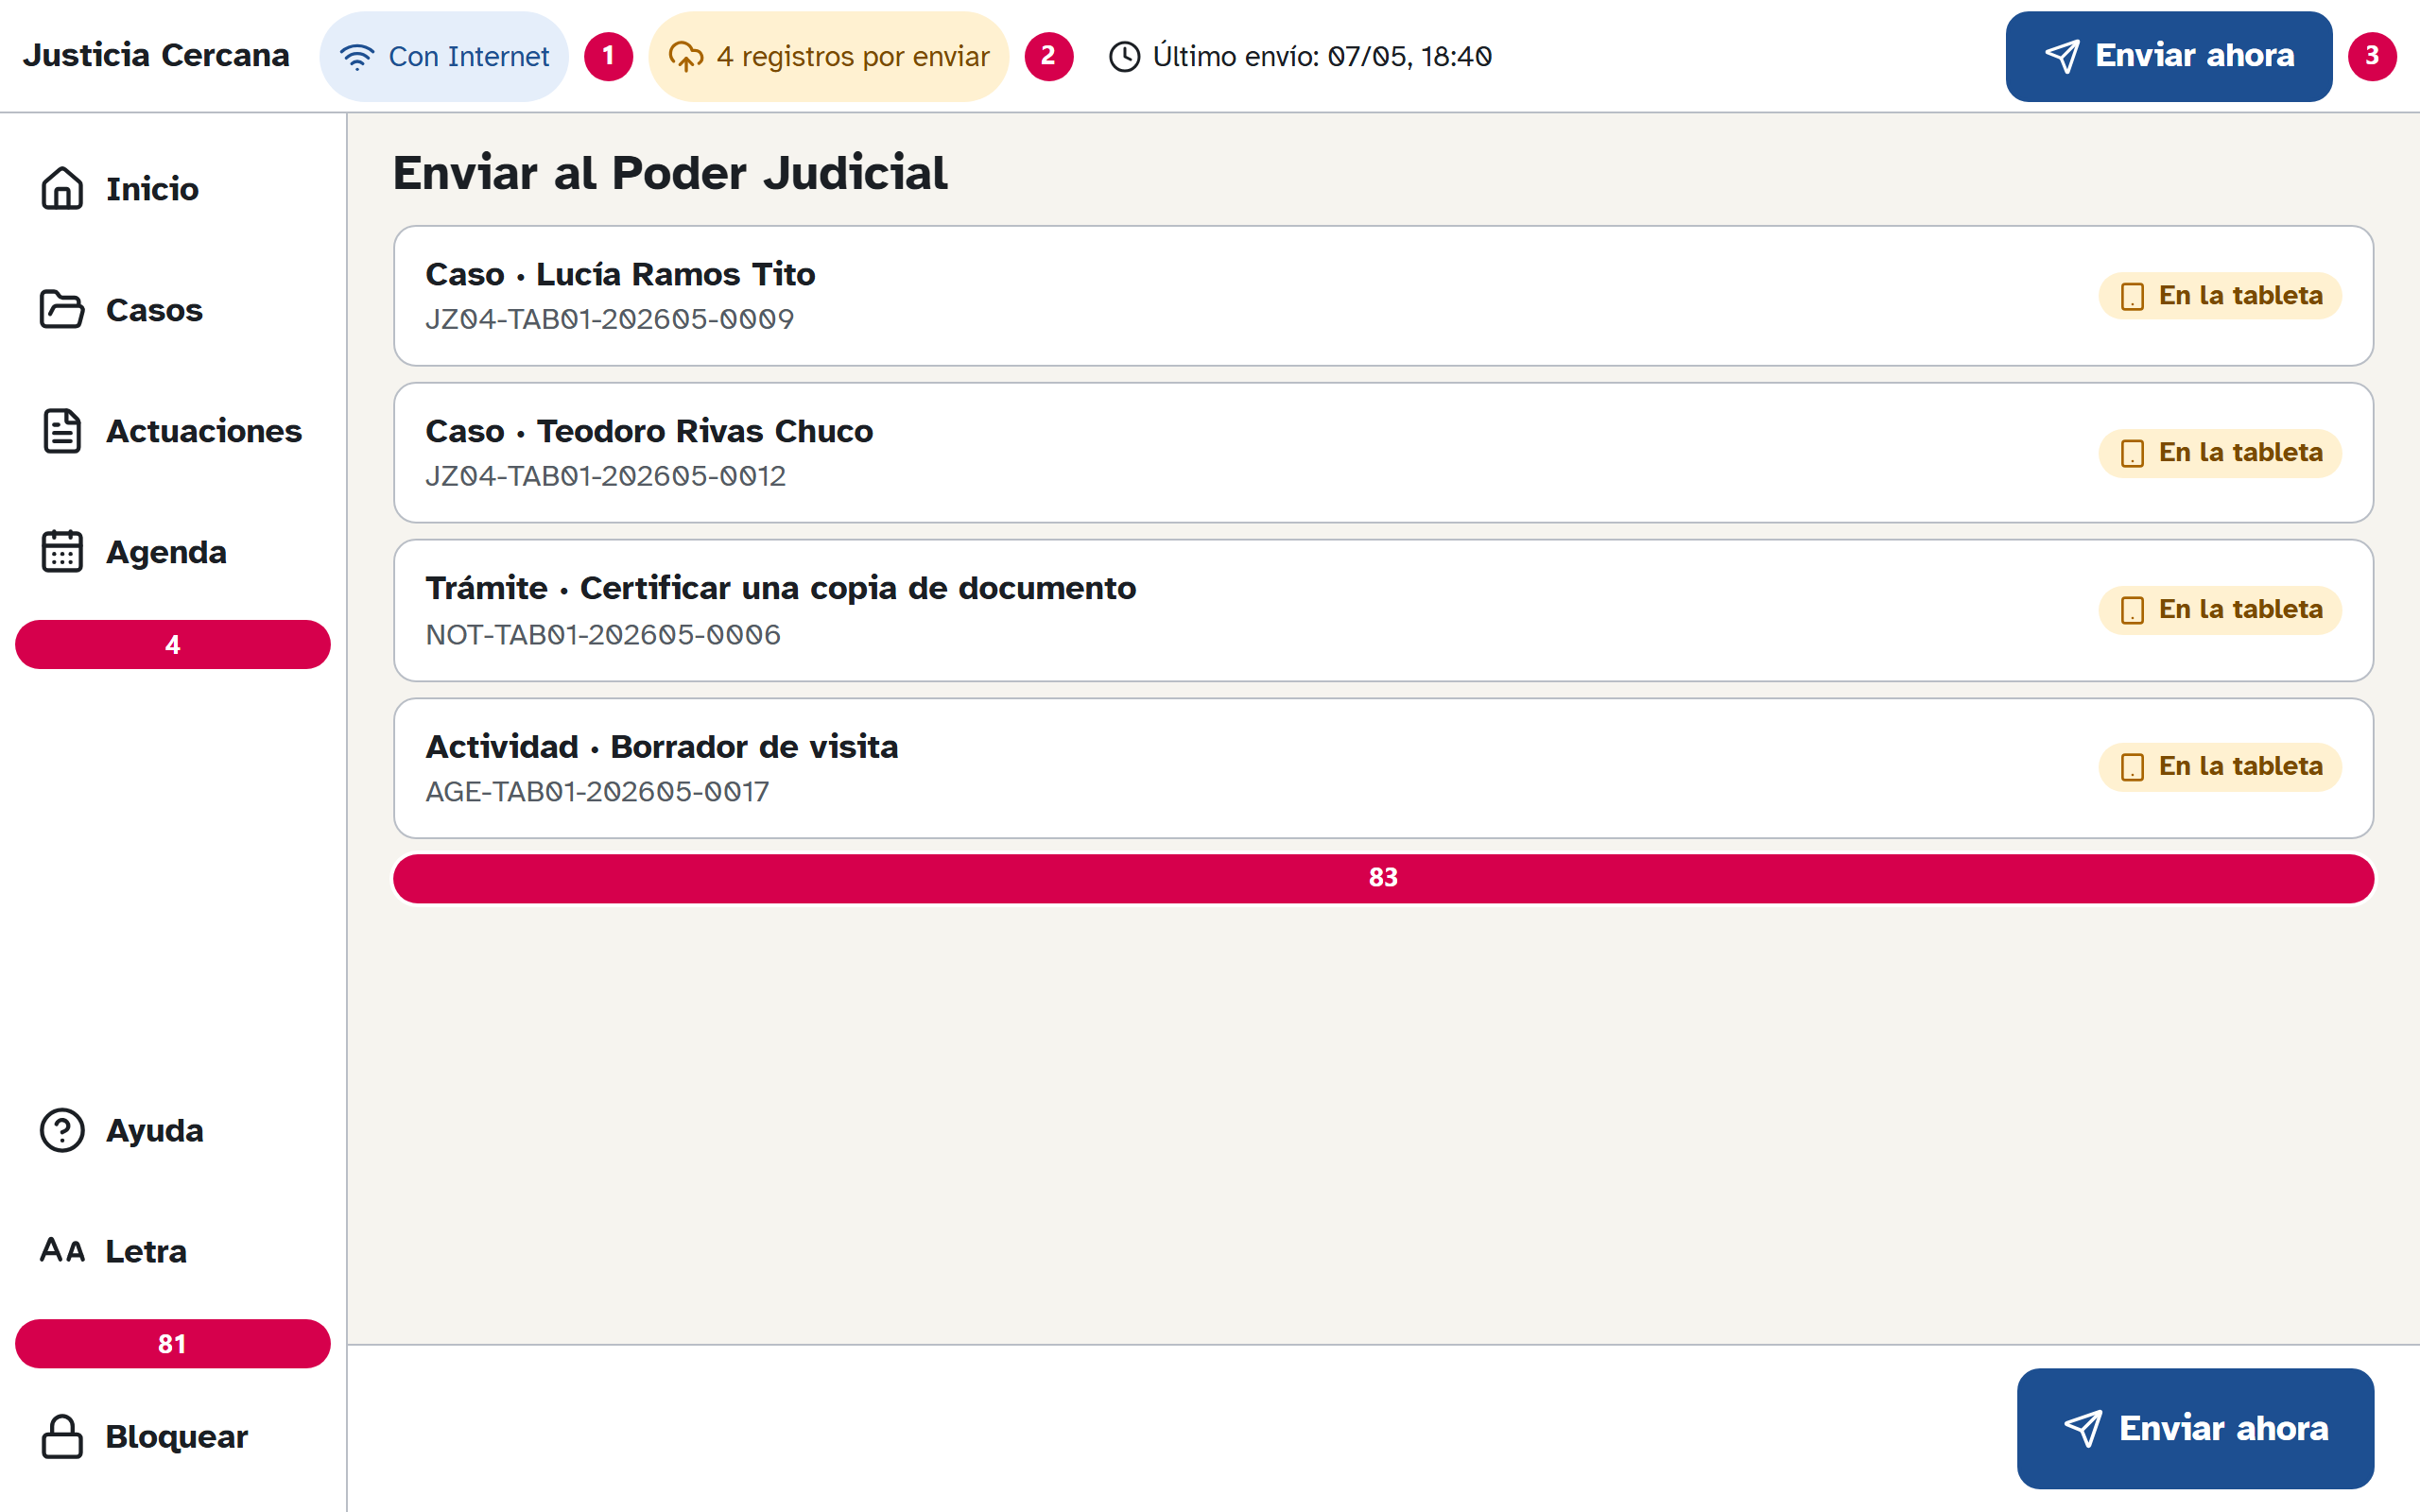
\includegraphics[width=\linewidth]{../../captures/ANOT_P-09_envio.png}\\[-2pt]{\footnotesize\raggedright\textbf{P-09.} Marcadores numerados = IDs de la matriz de justificación \emph{(Justificación de las decisiones)}\par}\end{minipage}\hfill
\begin{minipage}[t]{0.49\textwidth}\centering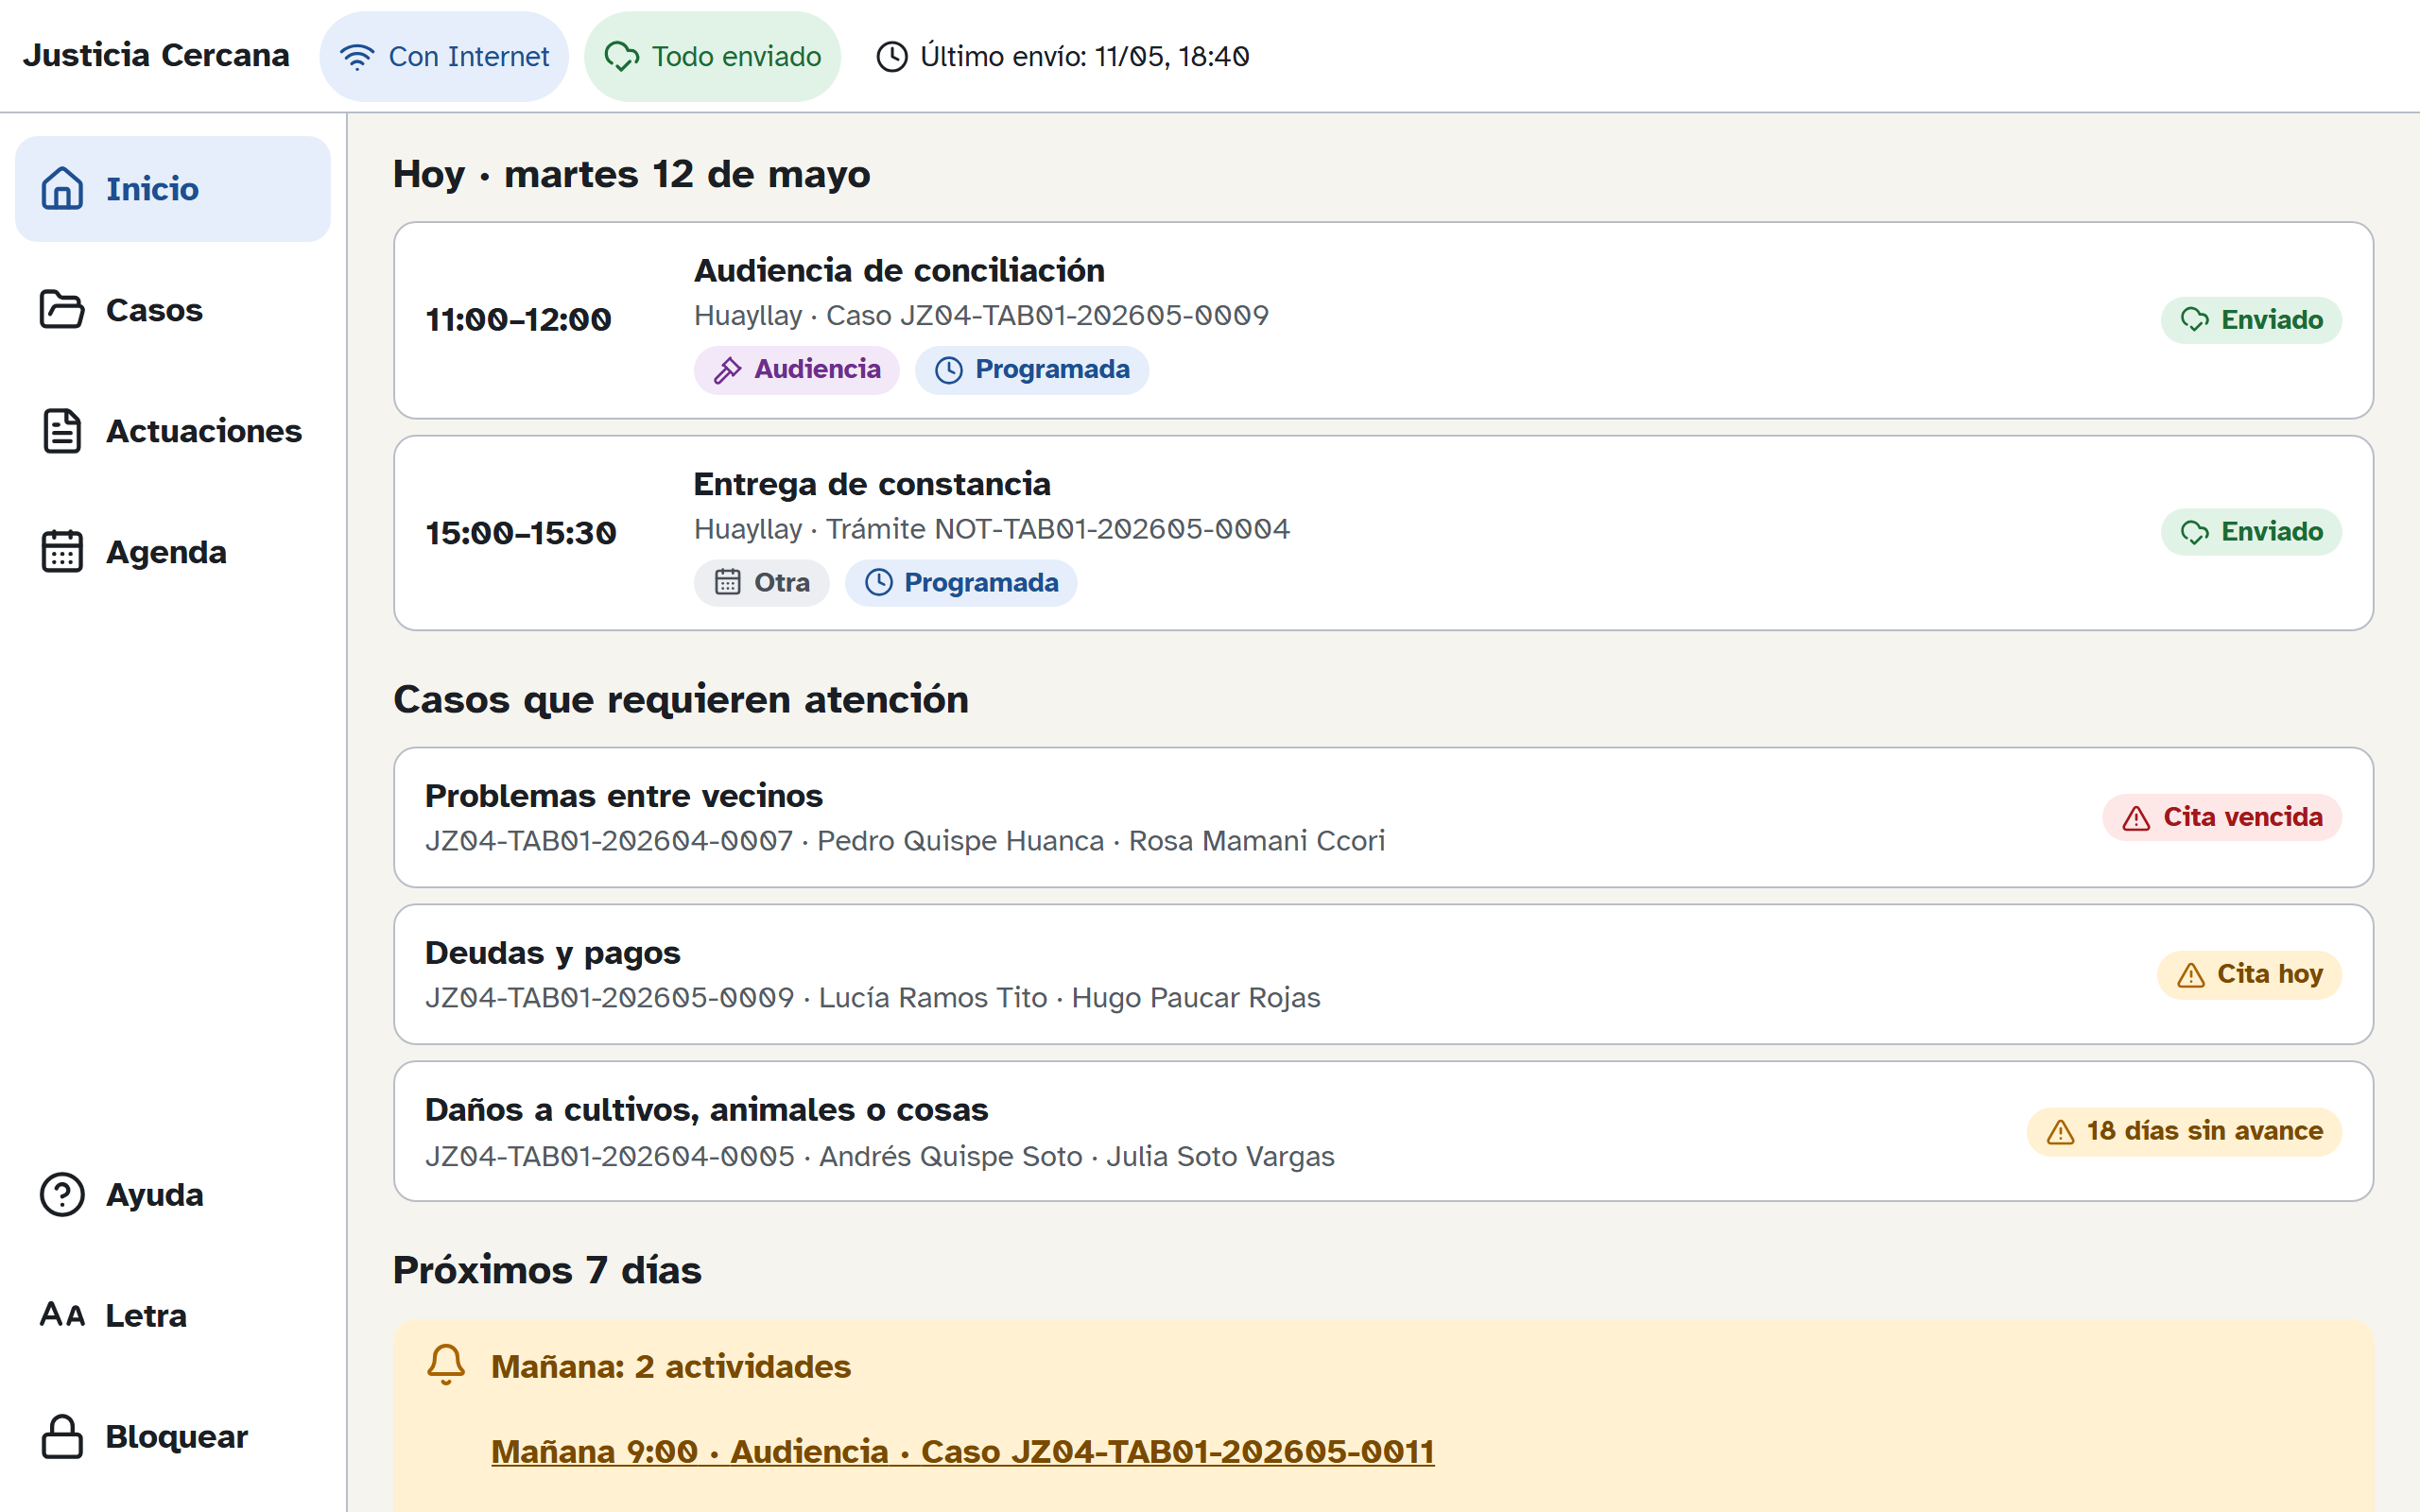
\includegraphics[width=\linewidth]{../../captures/G-01_barra-con-internet-todo-enviado.png}\\[-2pt]{\footnotesize\raggedright\textbf{Barra.} ``Con Internet'' (azul) · ``Todo enviado'' (verde) · último envío \emph{(Funcionamiento sin conexión)}\par}\end{minipage}\par\vspace{8pt}\noindent
\begin{minipage}[t]{0.49\textwidth}\centering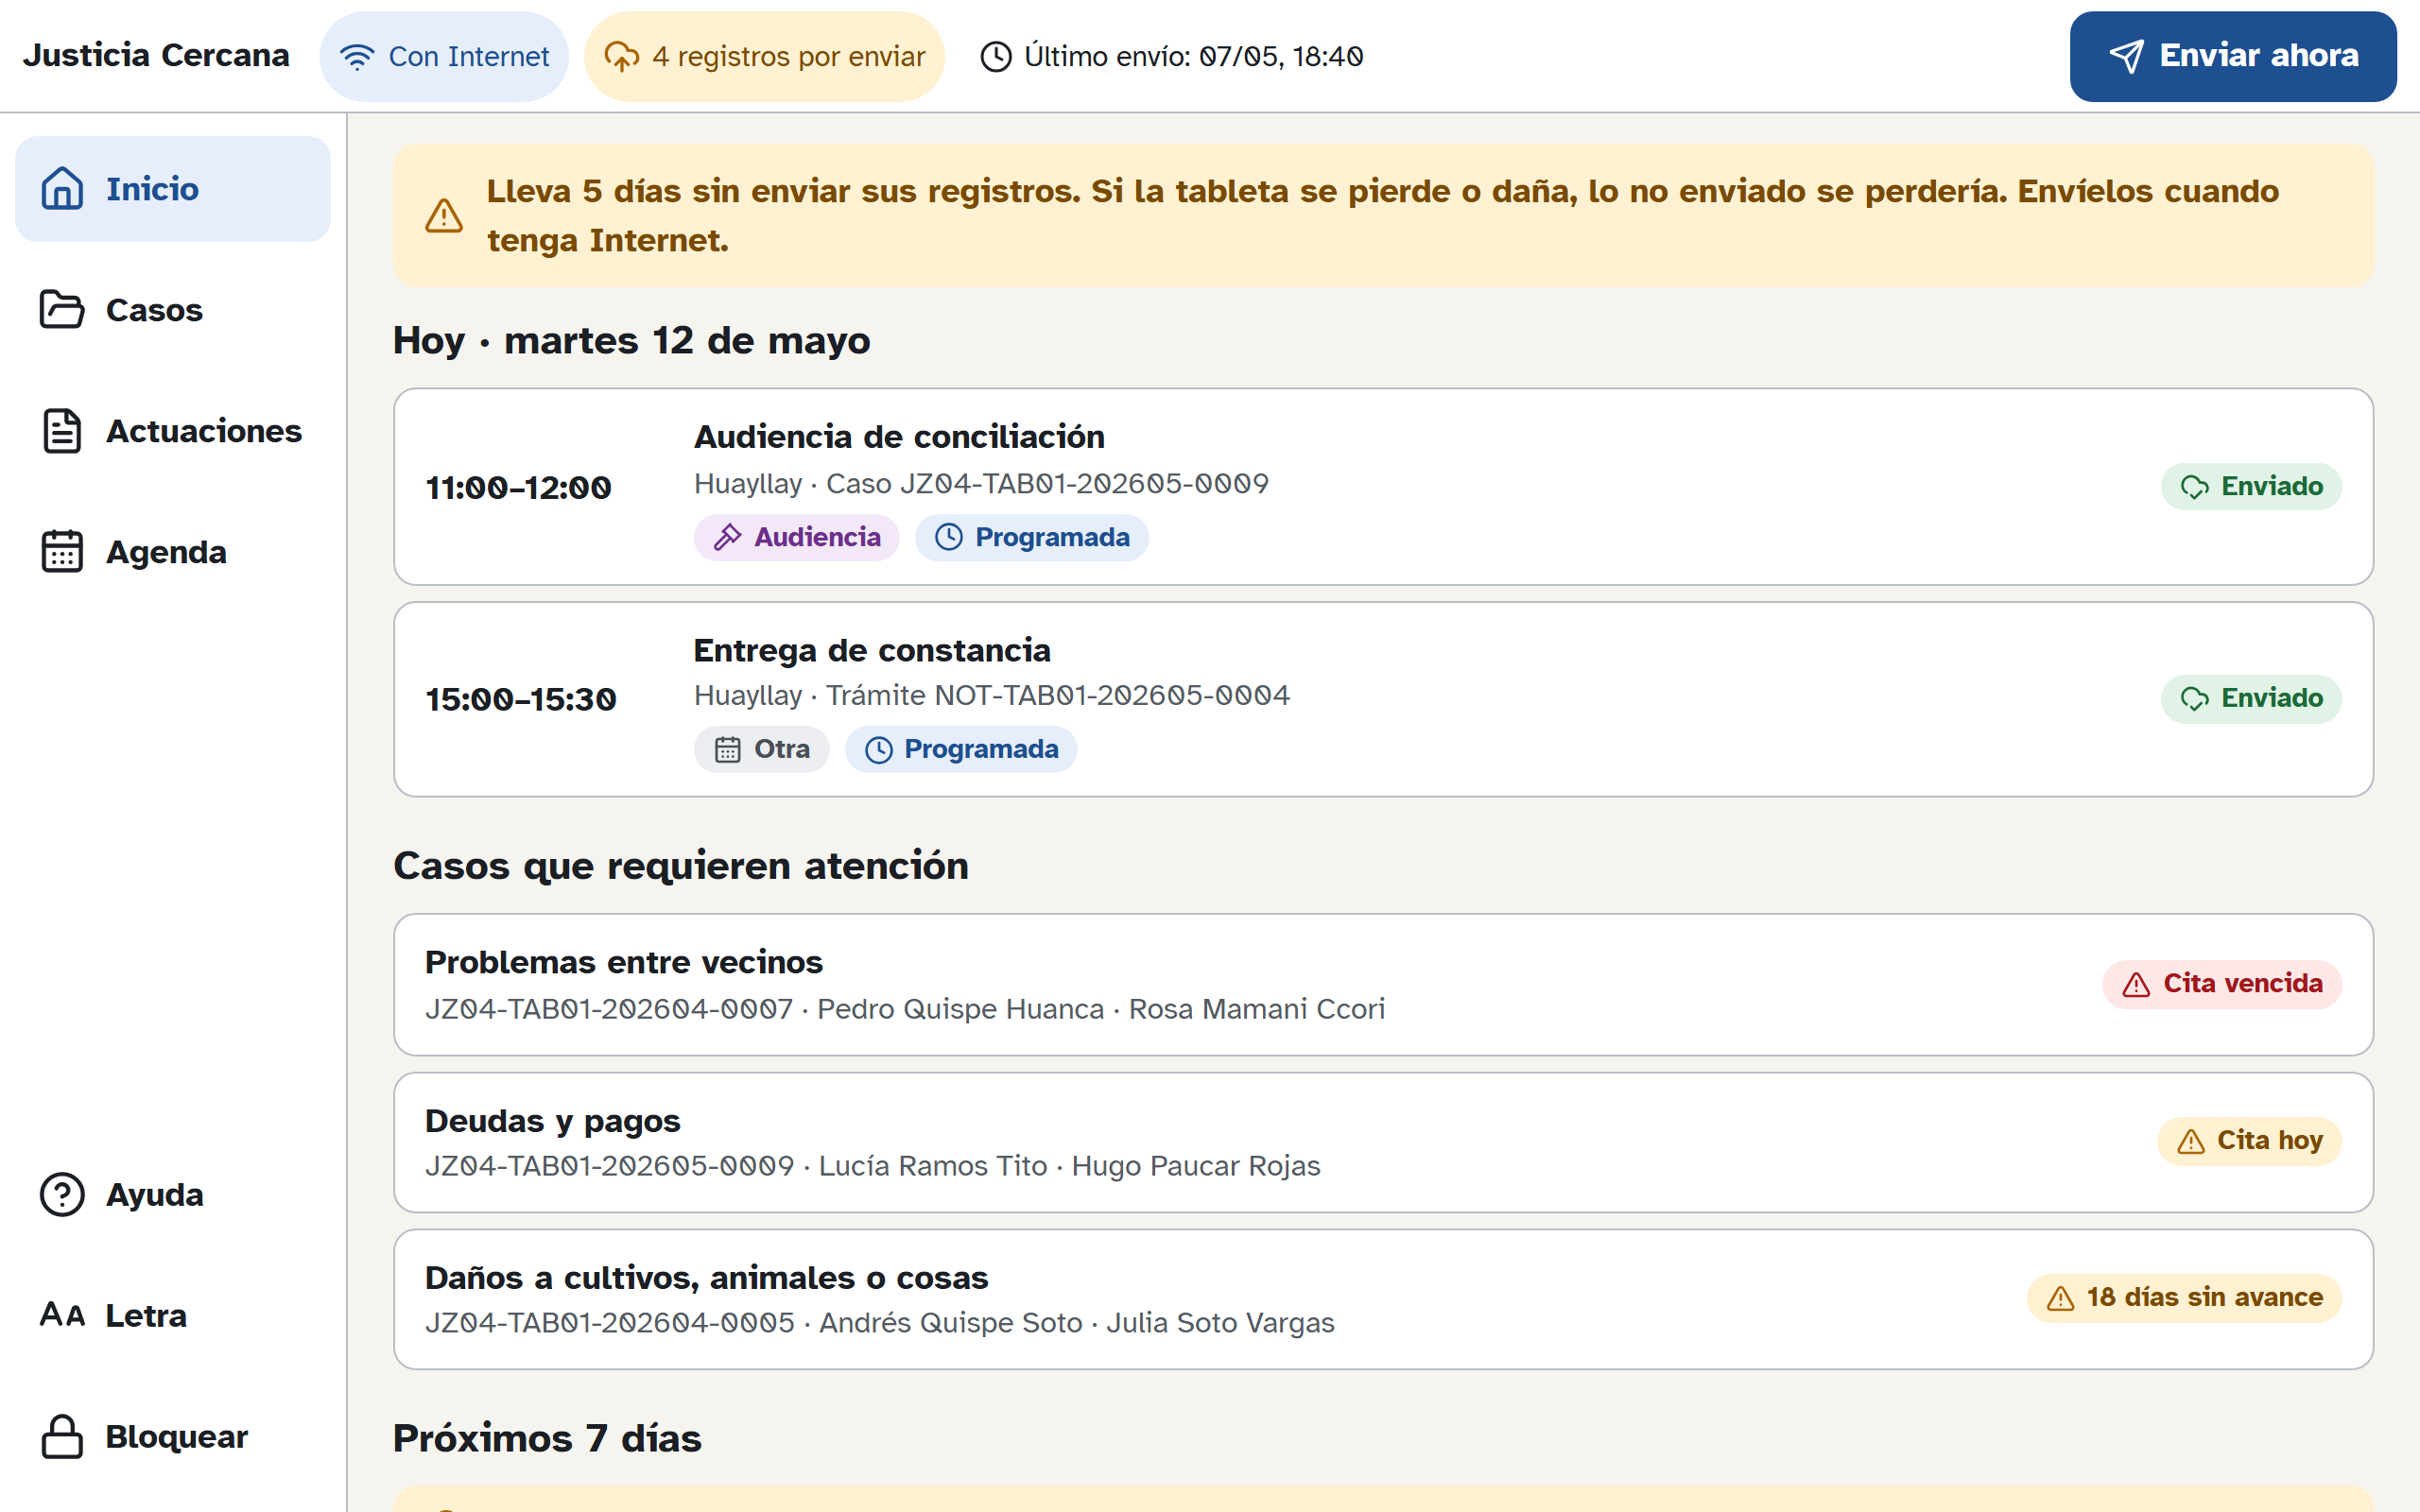
\includegraphics[width=\linewidth]{../../captures/G-02_barra-con-internet-pendientes-enviar-ahora.png}\\[-2pt]{\footnotesize\raggedright\textbf{Barra.} ``4 registros por enviar'' (ámbar) y botón visible [Enviar ahora] \emph{(Funcionamiento sin conexión)}\par}\end{minipage}\hfill
\begin{minipage}[t]{0.49\textwidth}\centering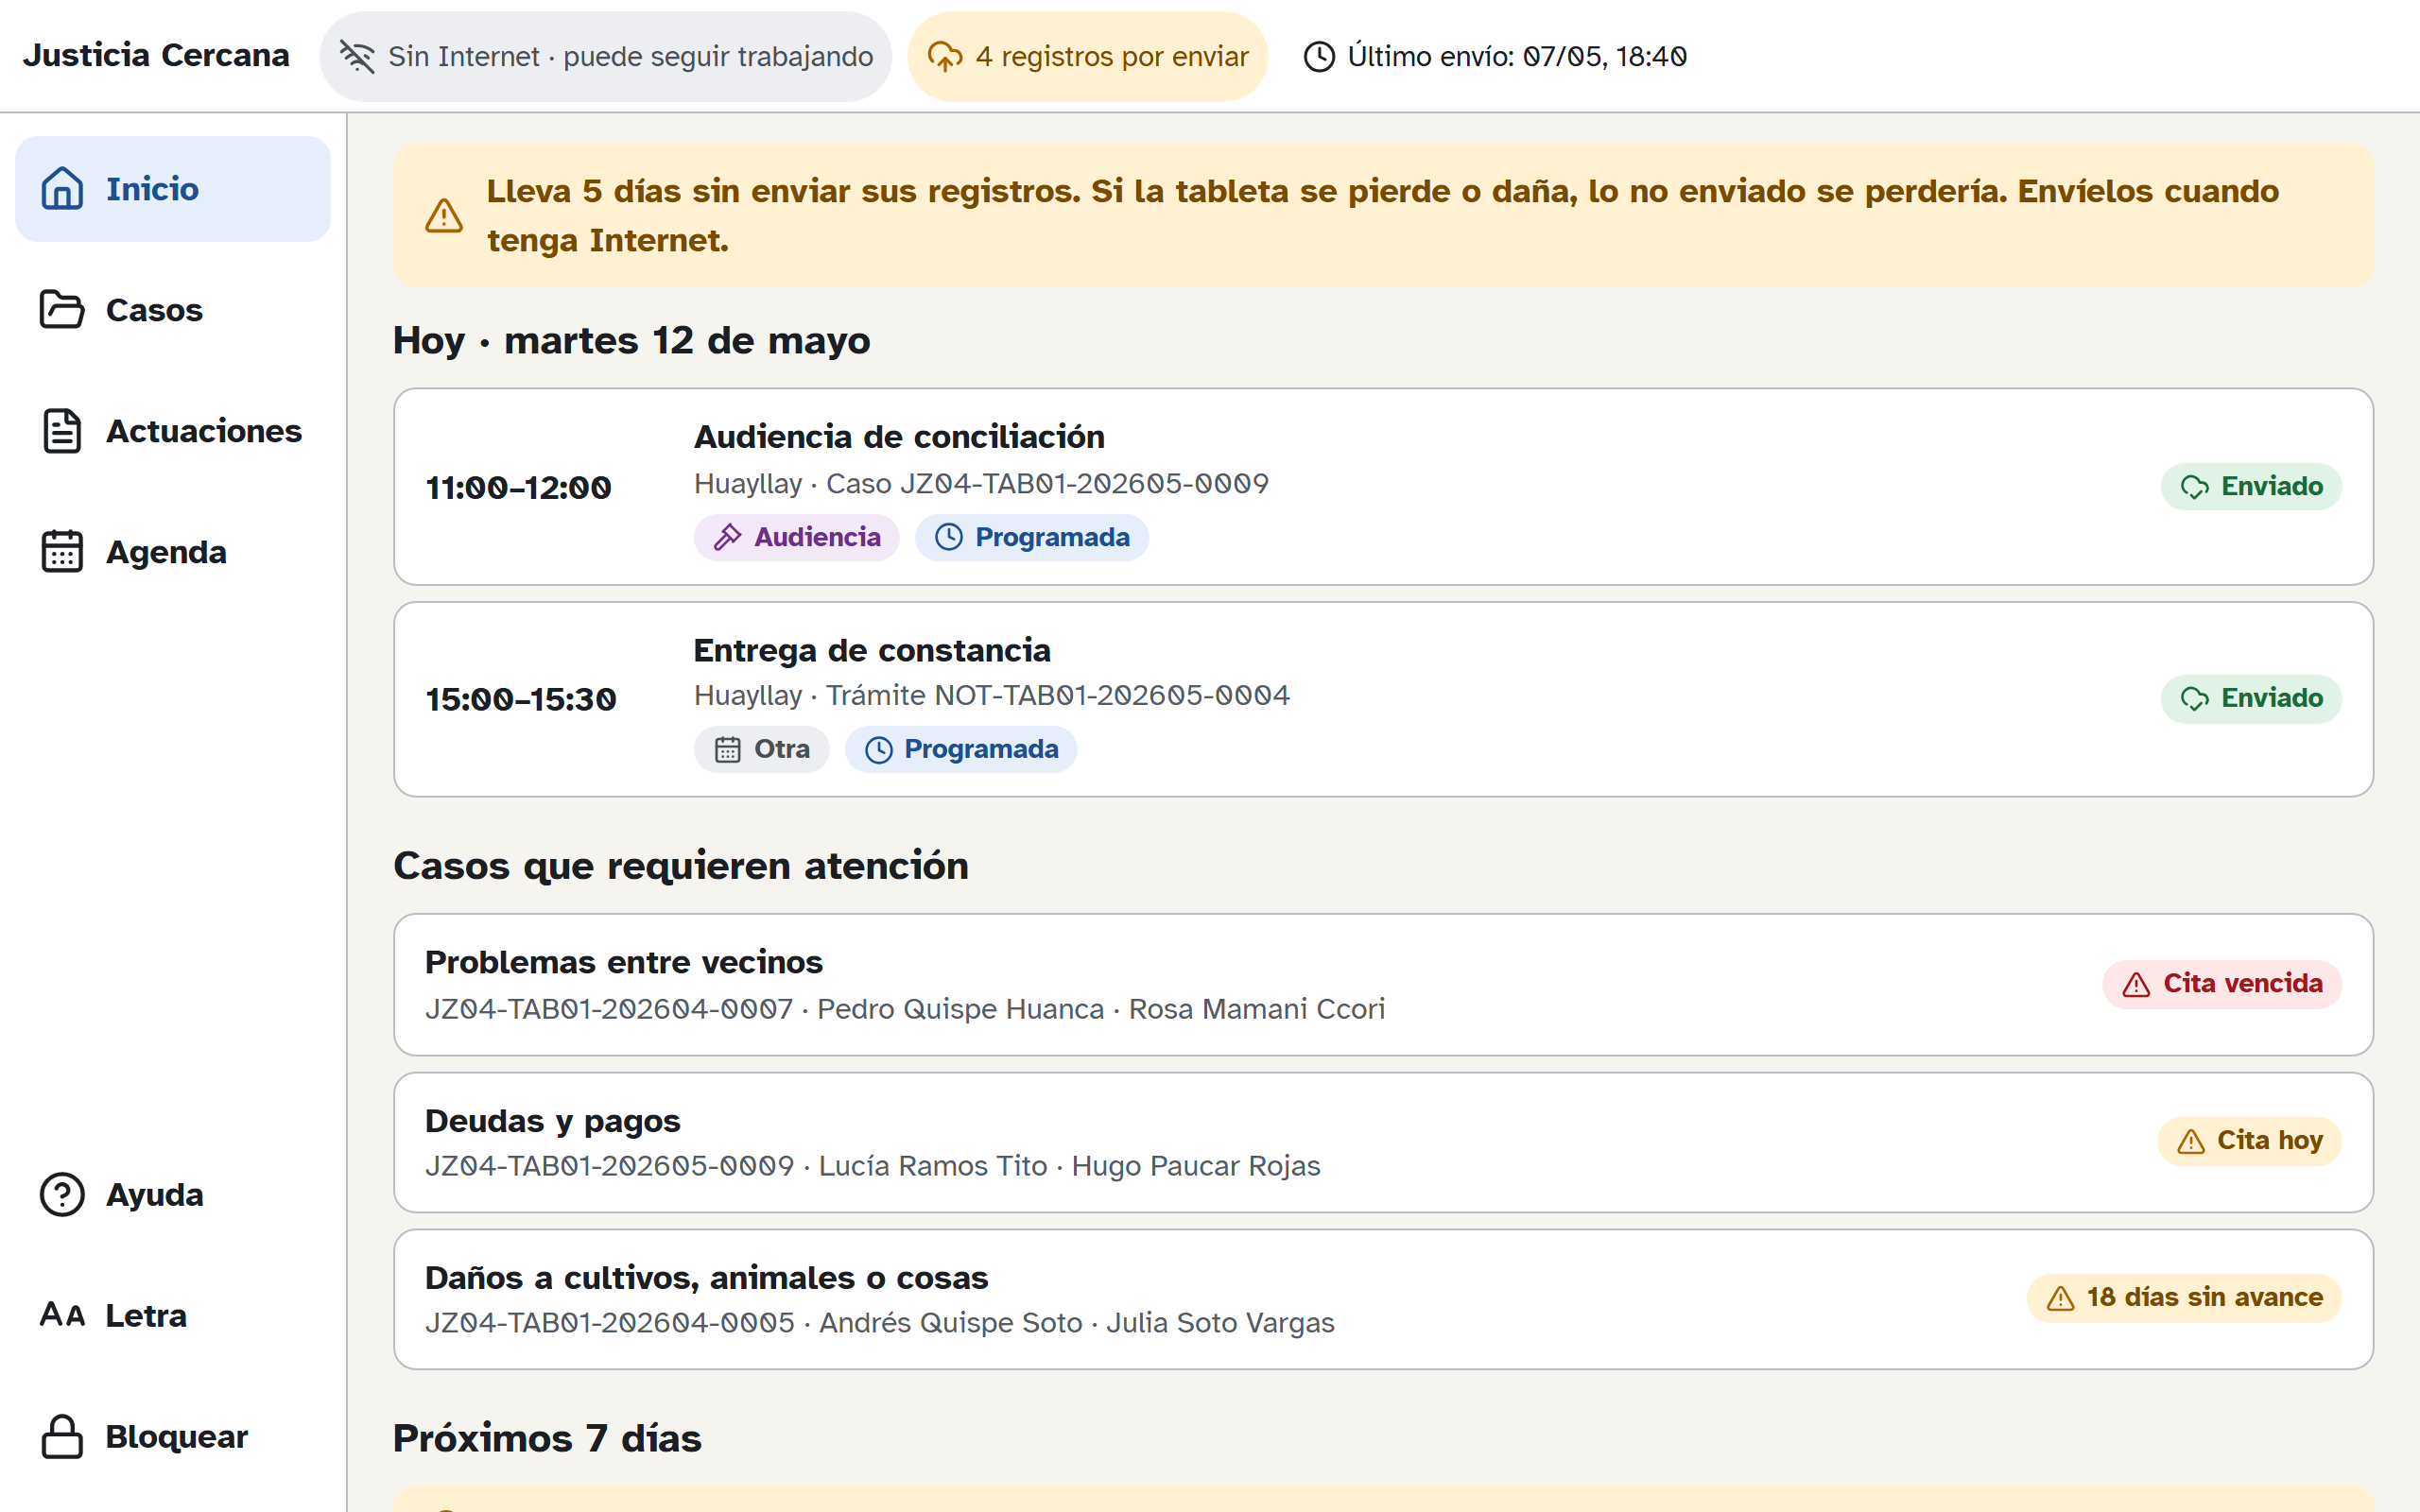
\includegraphics[width=\linewidth]{../../captures/G-03_barra-sin-internet-pendientes.png}\\[-2pt]{\footnotesize\raggedright\textbf{Barra.} ``Sin Internet'' en gris (nunca rojo) · ``4 registros por enviar''; sin [Enviar ahora] \emph{(Funcionamiento sin conexión)}\par}\end{minipage}\par\vspace{8pt}\noindent
\begin{minipage}[t]{0.49\textwidth}\centering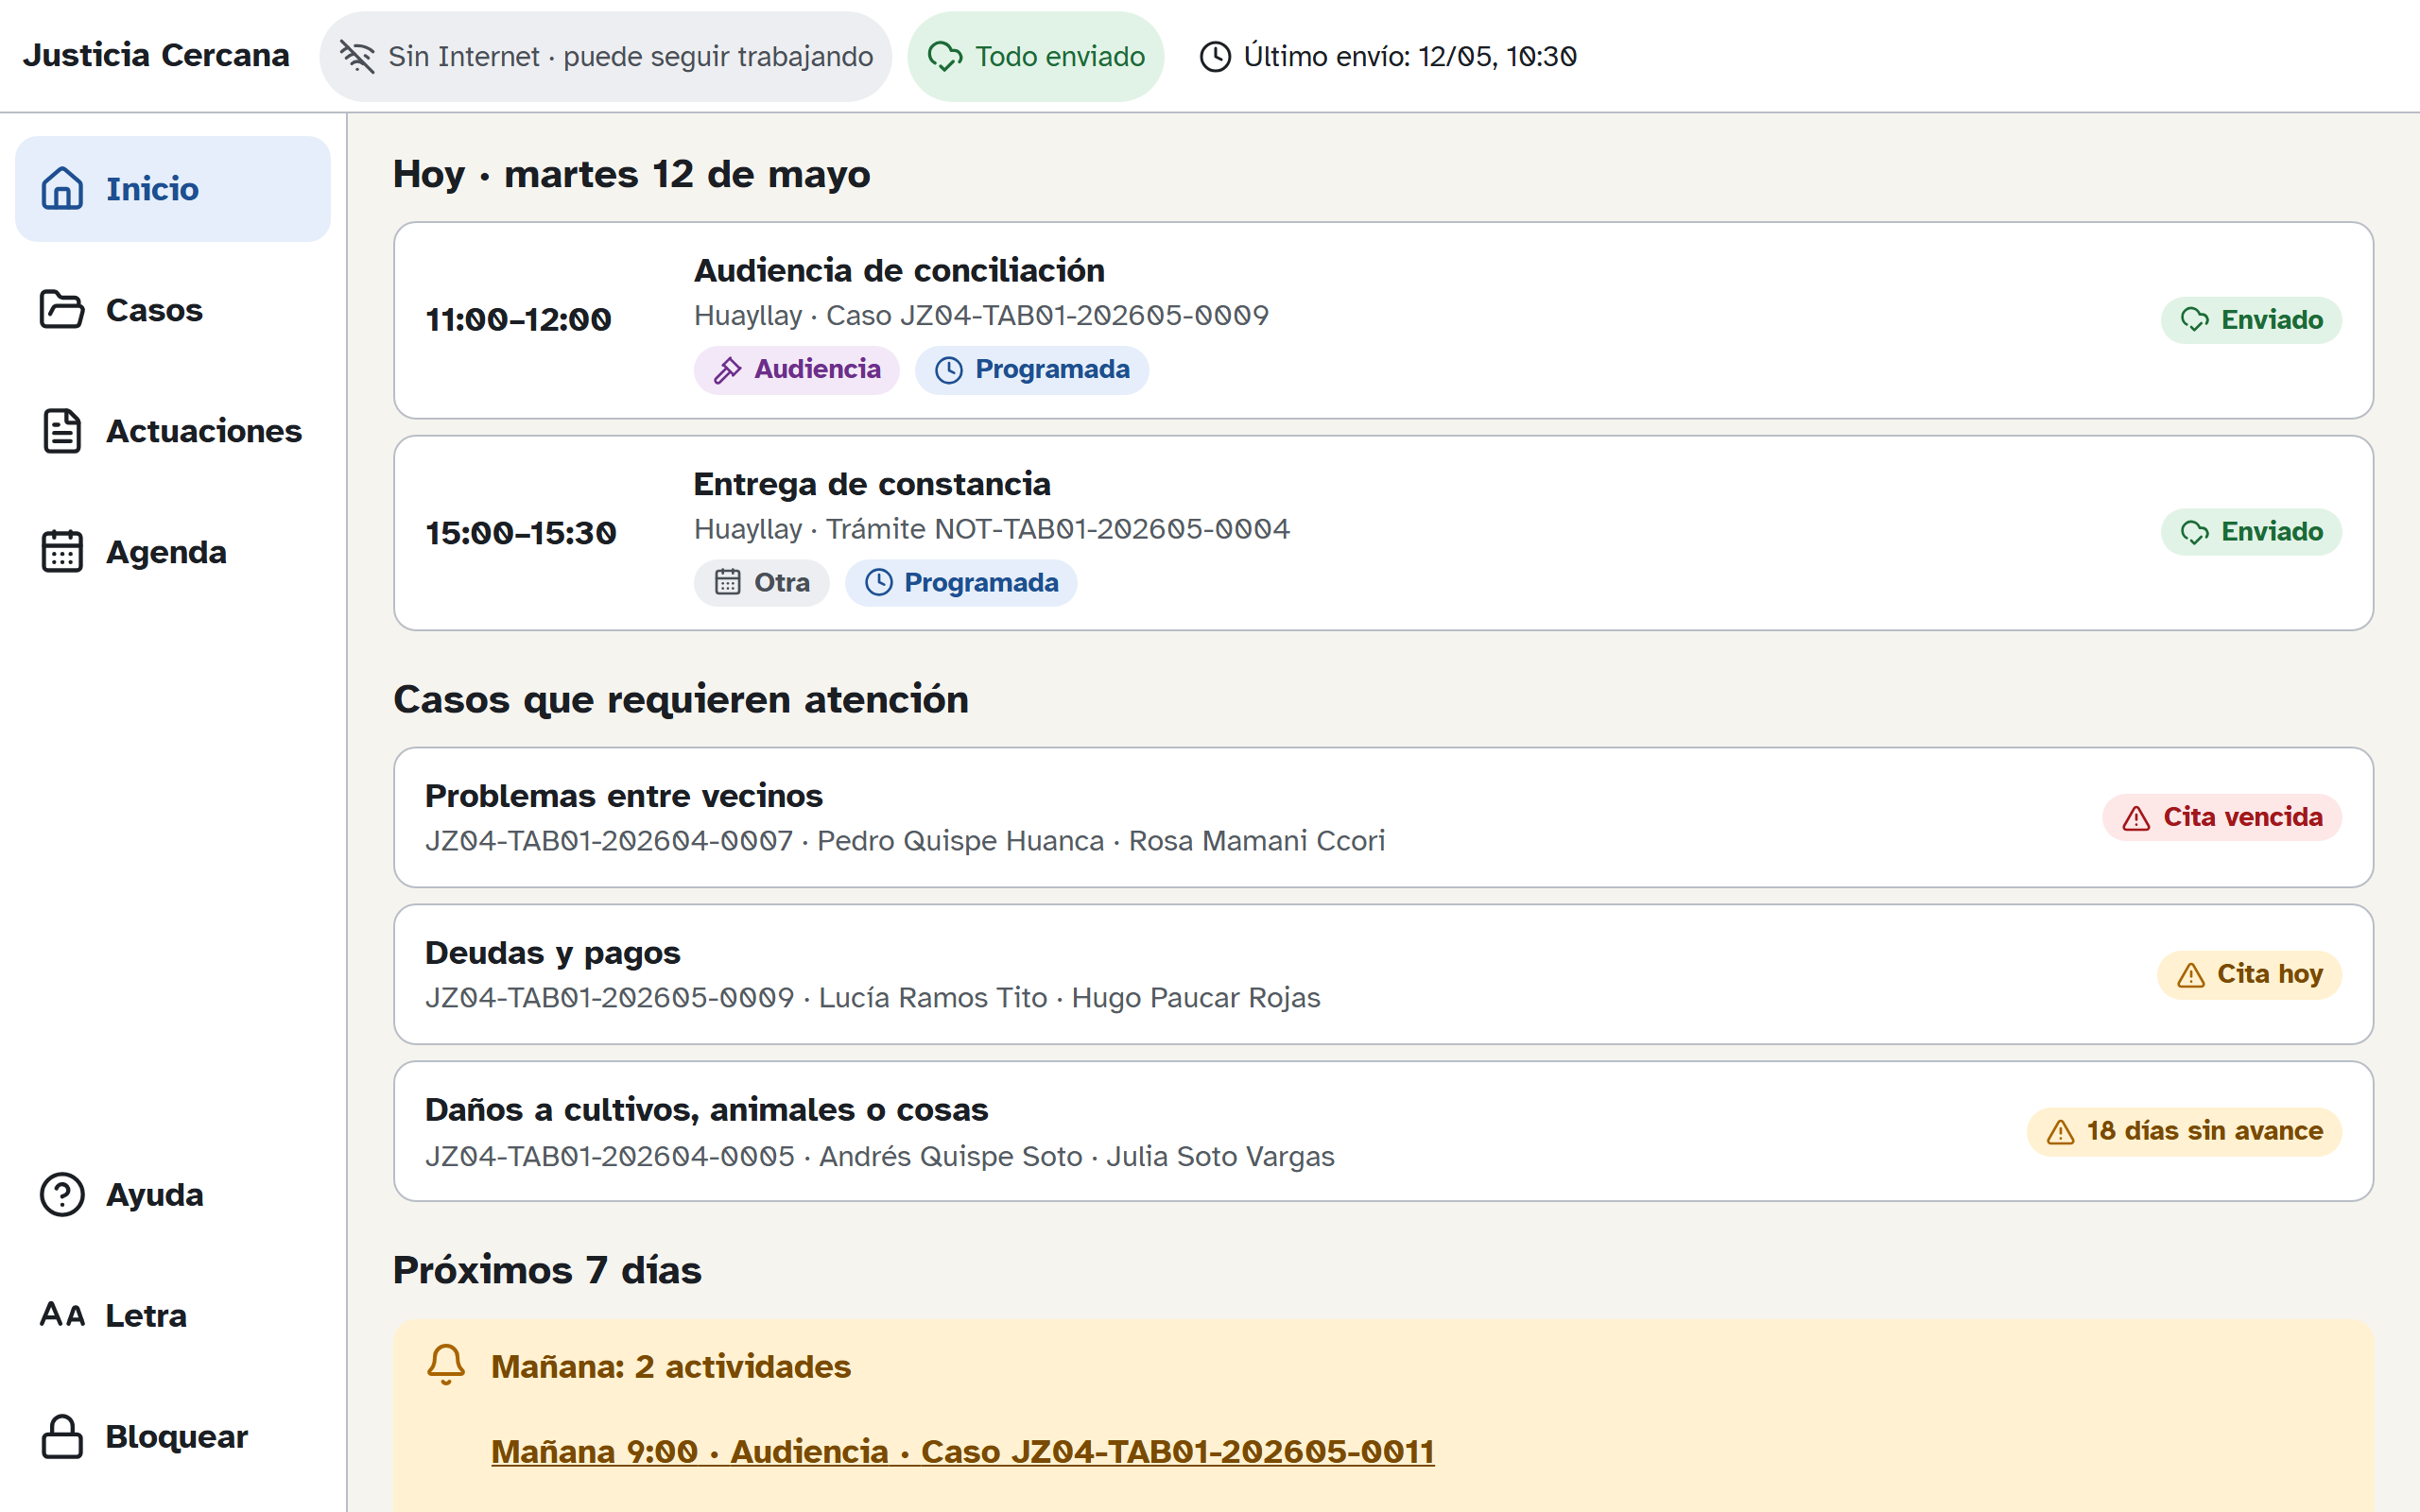
\includegraphics[width=\linewidth]{../../captures/G-04_barra-sin-internet-todo-enviado.png}\\[-2pt]{\footnotesize\raggedright\textbf{Barra.} ``Sin Internet'' (gris) · ``Todo enviado'' (verde) \emph{(Funcionamiento sin conexión)}\par}\end{minipage}\hfill
\begin{minipage}[t]{0.49\textwidth}\centering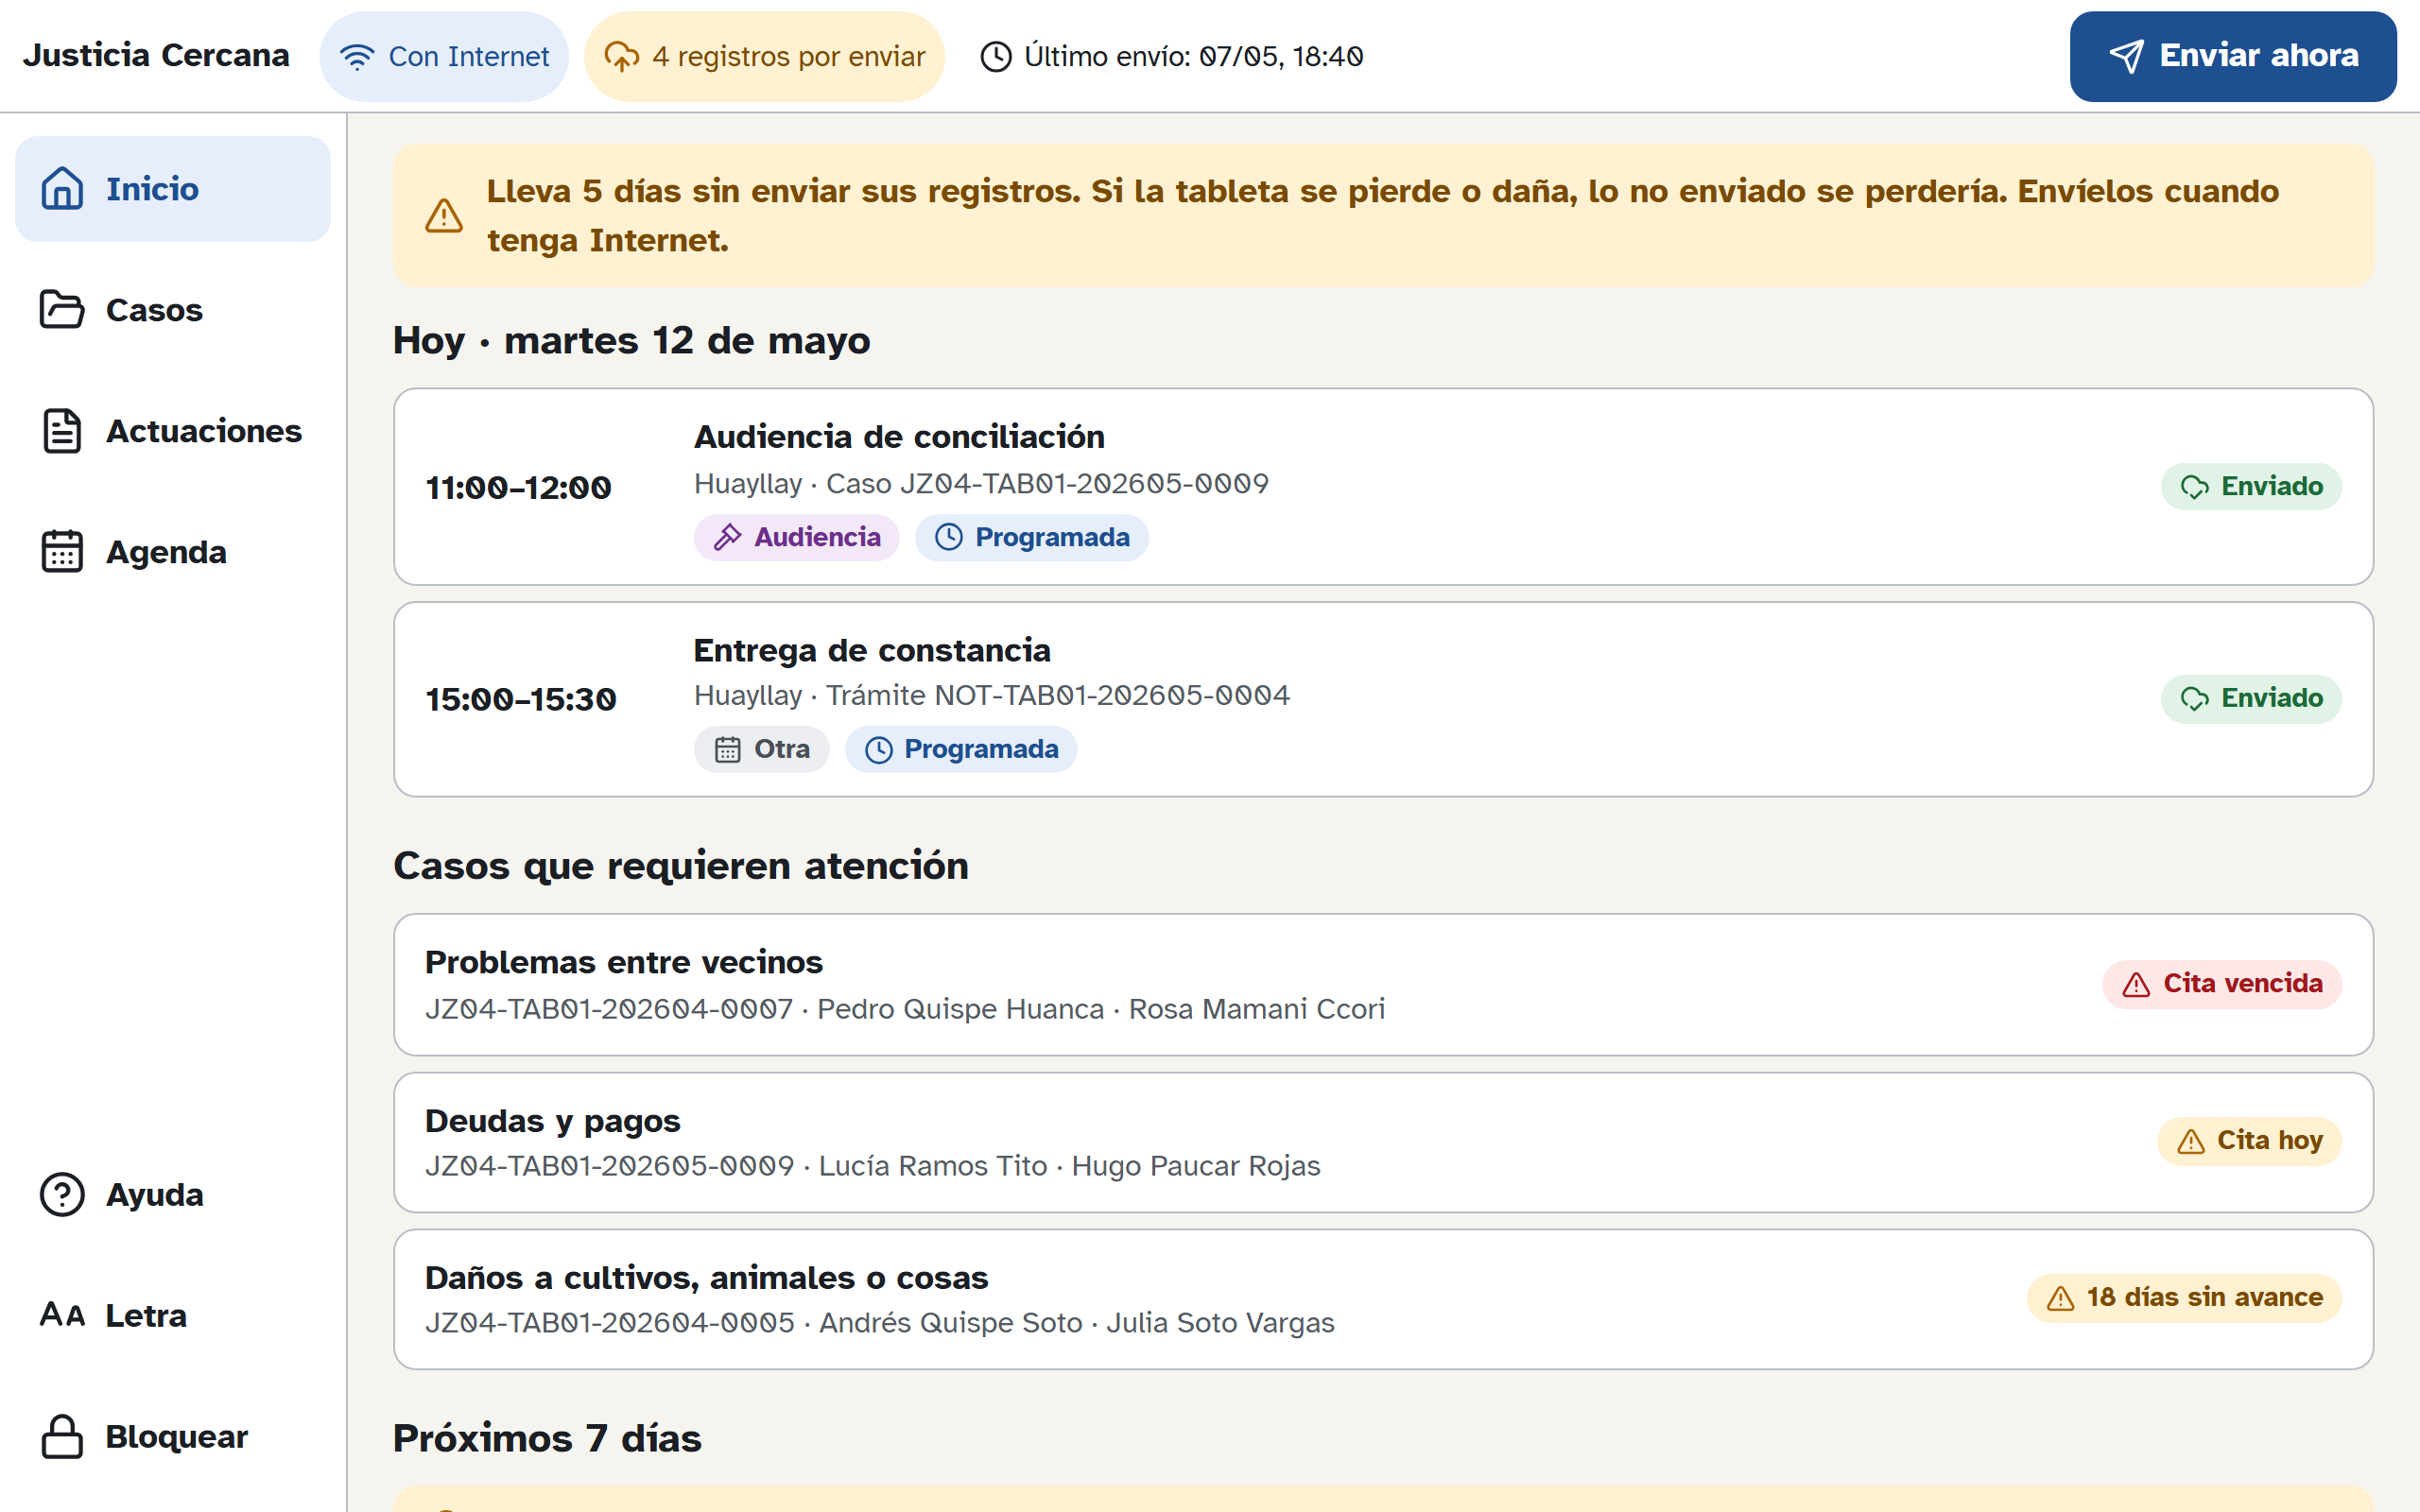
\includegraphics[width=\linewidth]{../../captures/G-05_recordatorio-dias-sin-enviar.png}\\[-2pt]{\footnotesize\raggedright\textbf{P-01.} Recordatorio ``Lleva 5 días sin enviar sus registros…'' (seed=mixed) \emph{(Funcionamiento sin conexión)}\par}\end{minipage}\par\vspace{8pt}\noindent
\begin{minipage}[t]{0.49\textwidth}\centering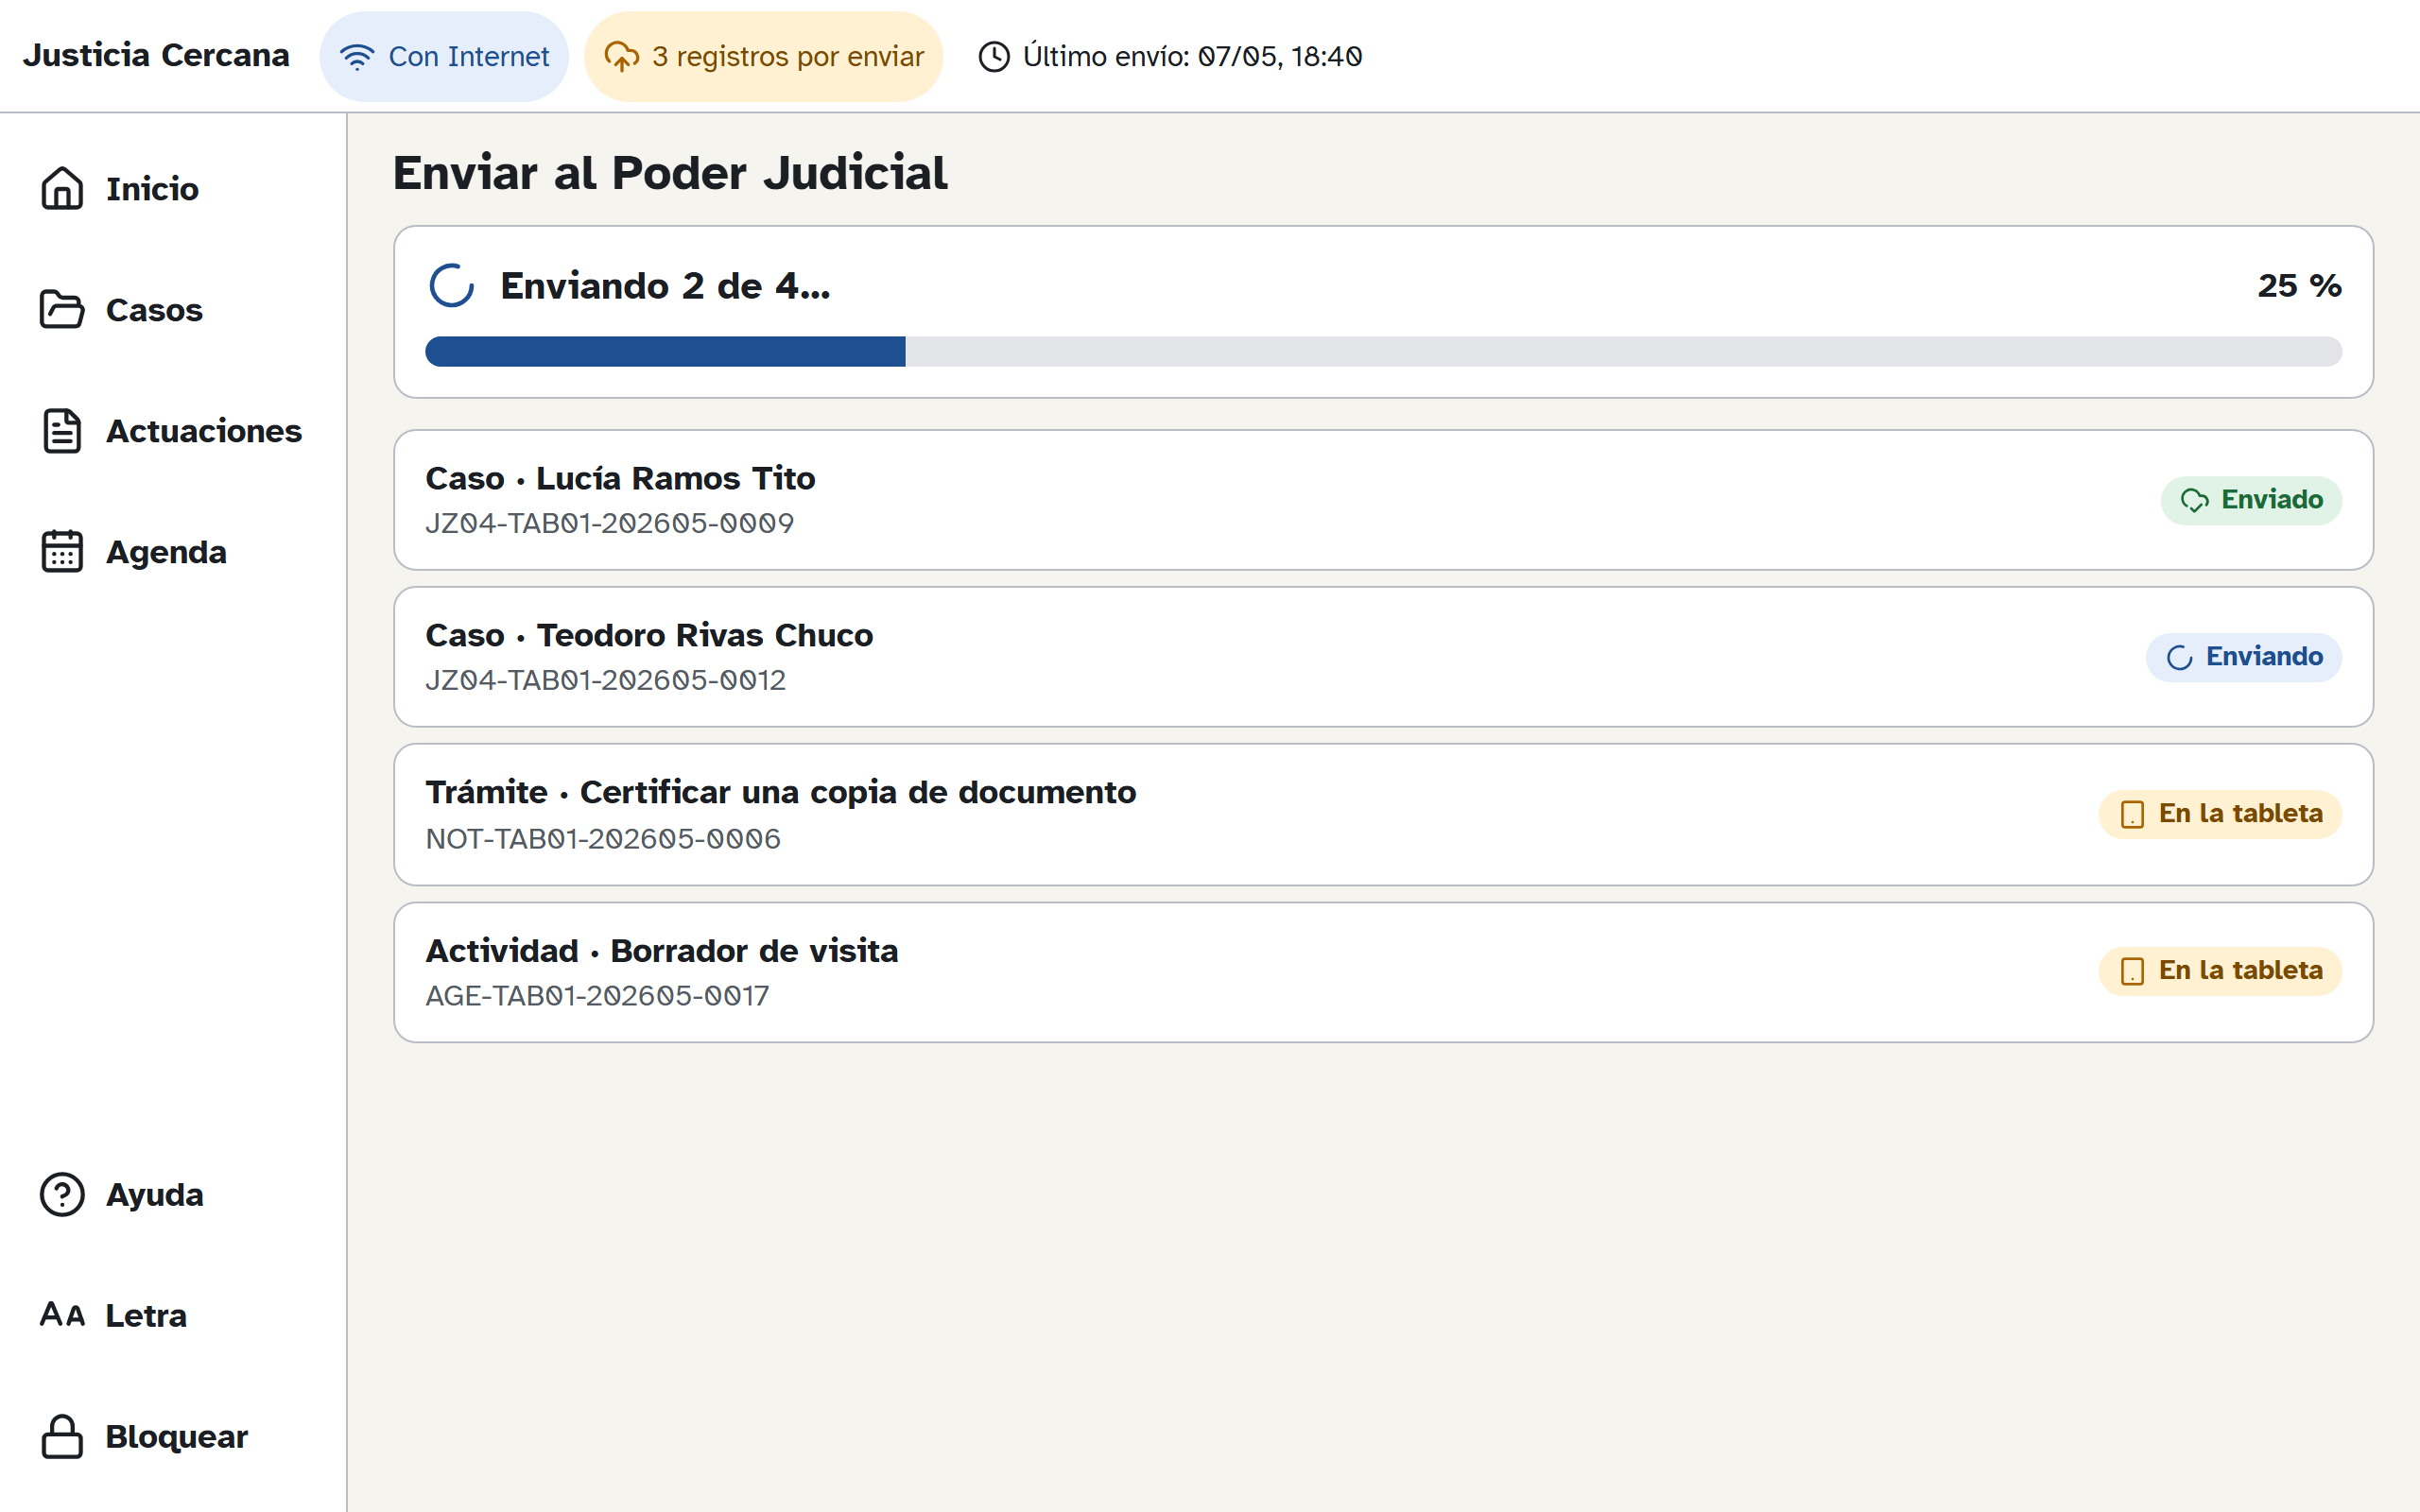
\includegraphics[width=\linewidth]{../../captures/G-06_progreso-envio.png}\\[-2pt]{\footnotesize\raggedright\textbf{P-09.} Progreso ``Enviando 2 de 4…'' con barra al 50 \% y estado por registro (freeze=1) \emph{(Funcionamiento sin conexión)}\par}\end{minipage}\hfill
\begin{minipage}[t]{0.49\textwidth}\centering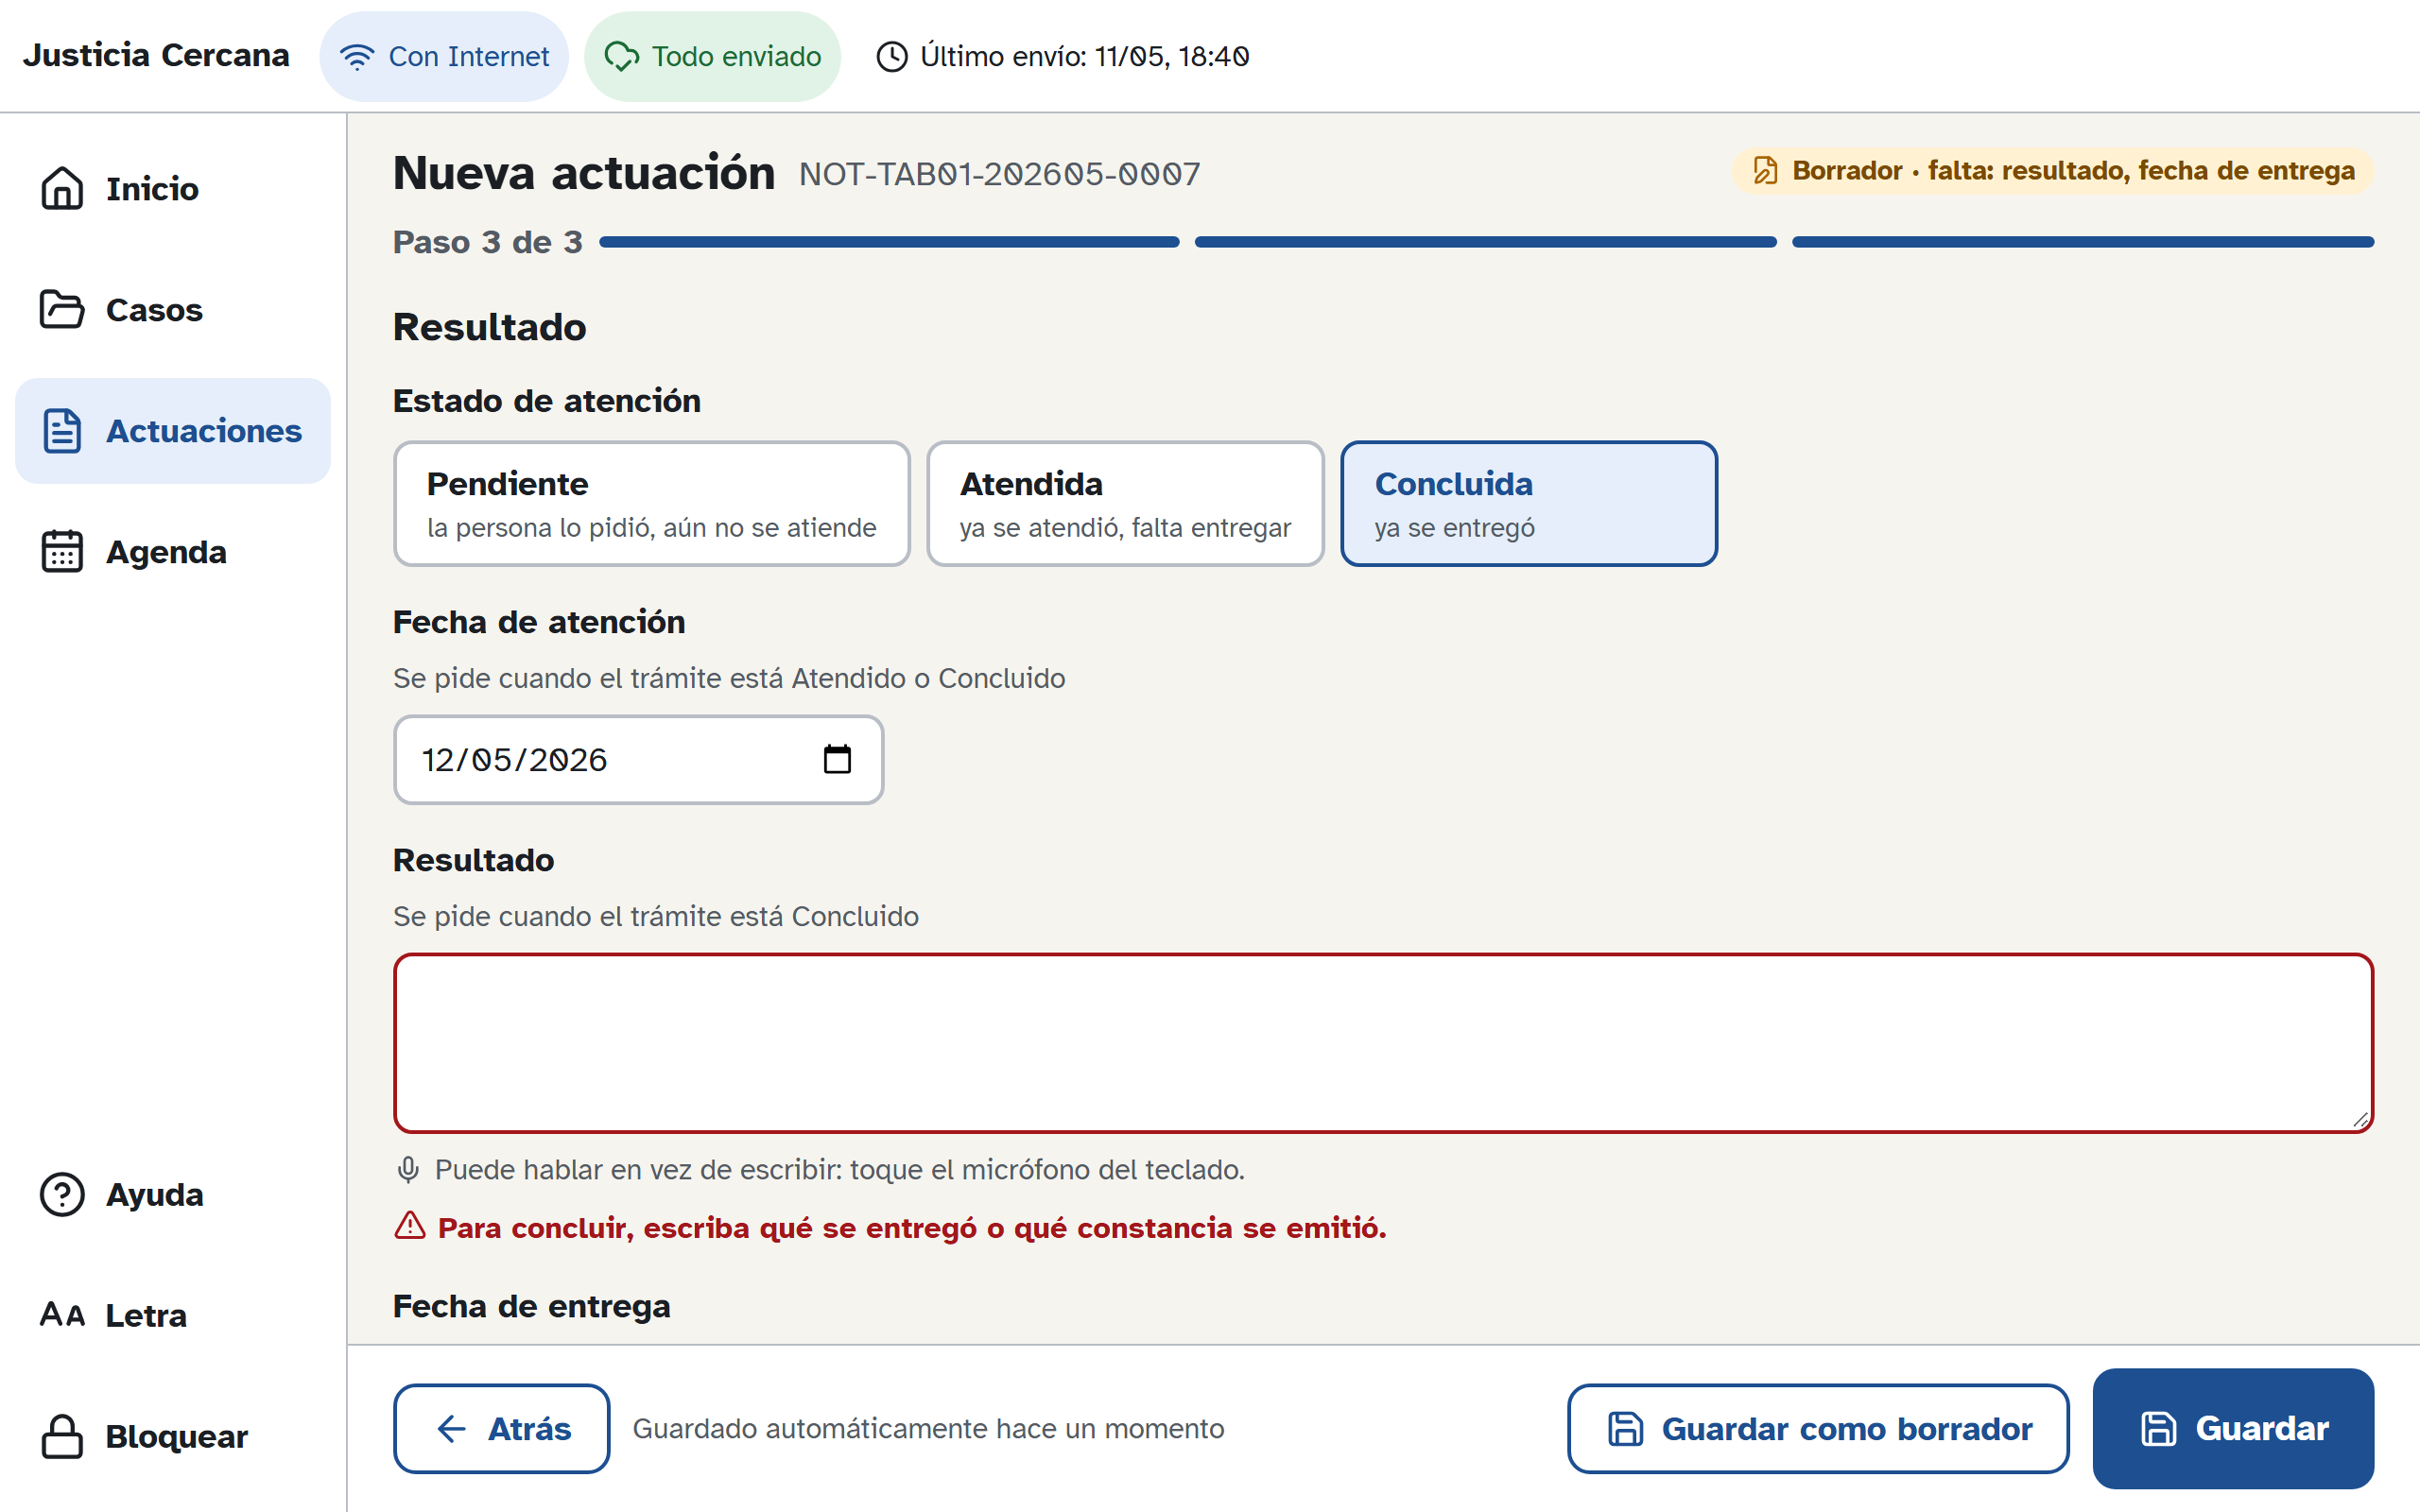
\includegraphics[width=\linewidth]{../../captures/G-07_opcional-y-condicionales.png}\\[-2pt]{\footnotesize\raggedright\textbf{P-06.} Etiquetas ``(opcional)'' y líneas de campos condicionales (``Se pide cuando…'') \emph{(Principios de diseño y heurísticas)}\par}\end{minipage}\par\vspace{8pt}\noindent
\begin{minipage}[t]{0.49\textwidth}\centering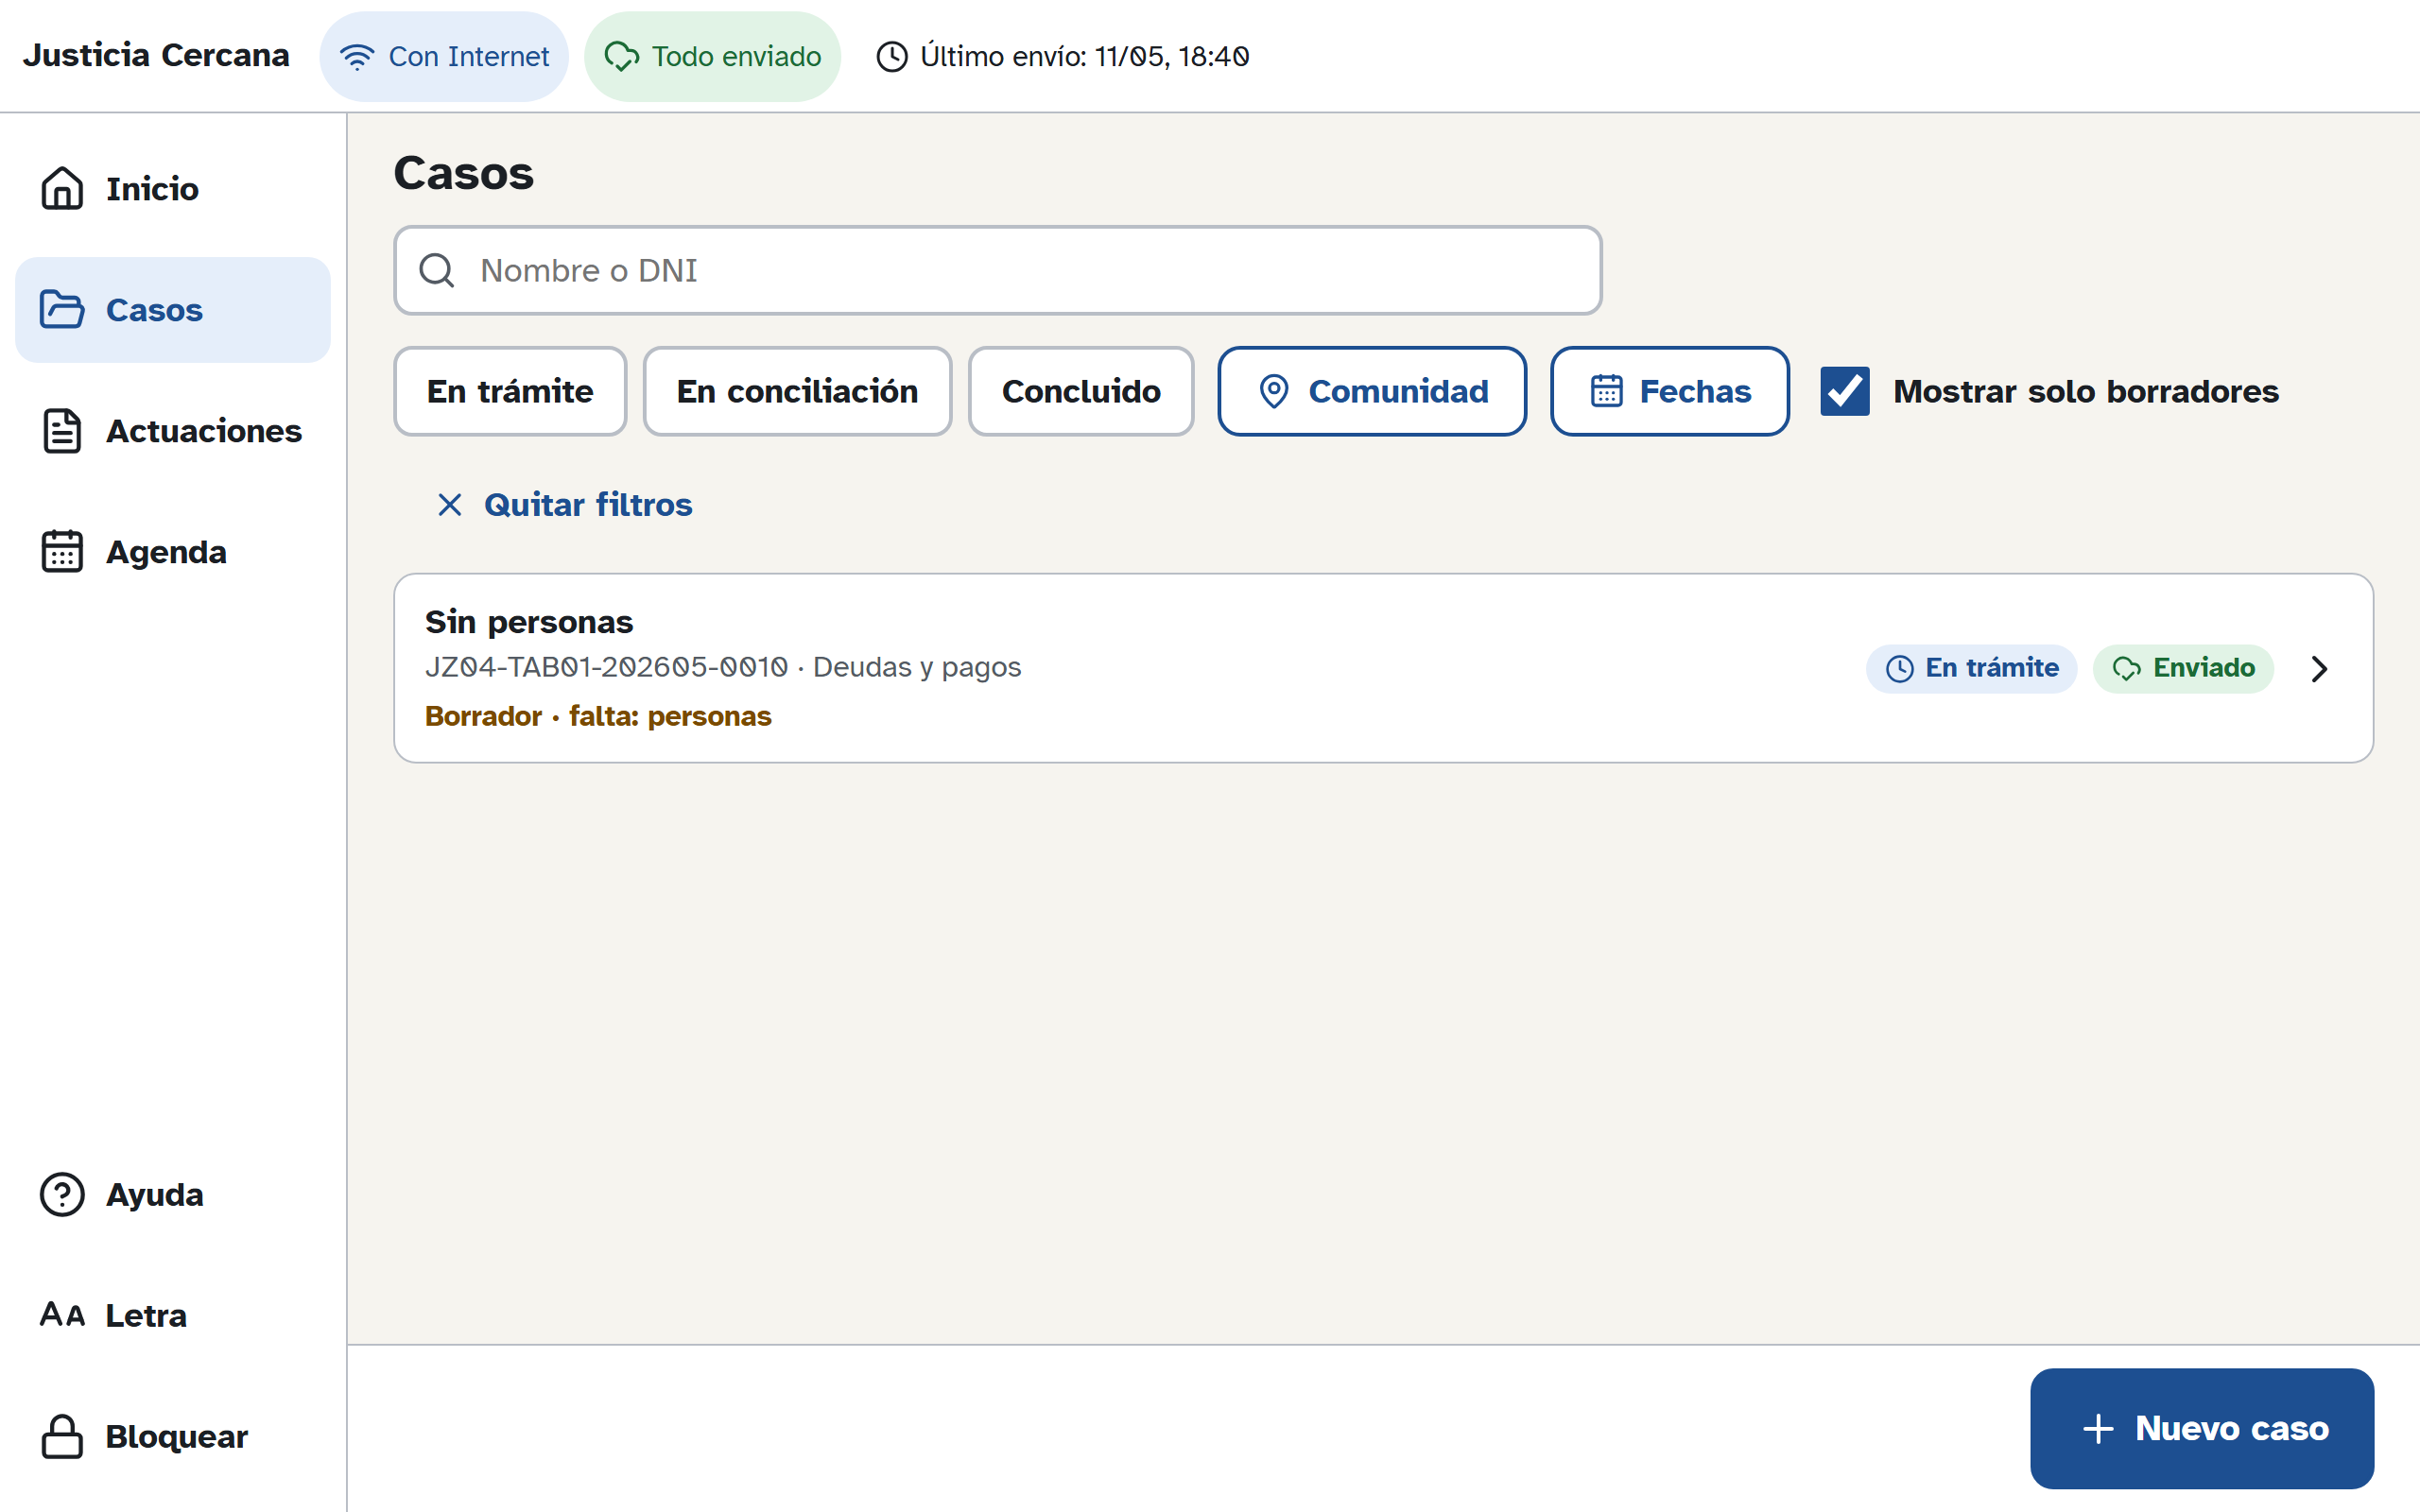
\includegraphics[width=\linewidth]{../../captures/G-08_borrador-casos.png}\\[-2pt]{\footnotesize\raggedright\textbf{P-02.} ``Borrador · falta: personas'' y casilla ``Mostrar solo borradores'' (casos) \emph{(Principios de diseño y heurísticas)}\par}\end{minipage}\hfill
\begin{minipage}[t]{0.49\textwidth}\centering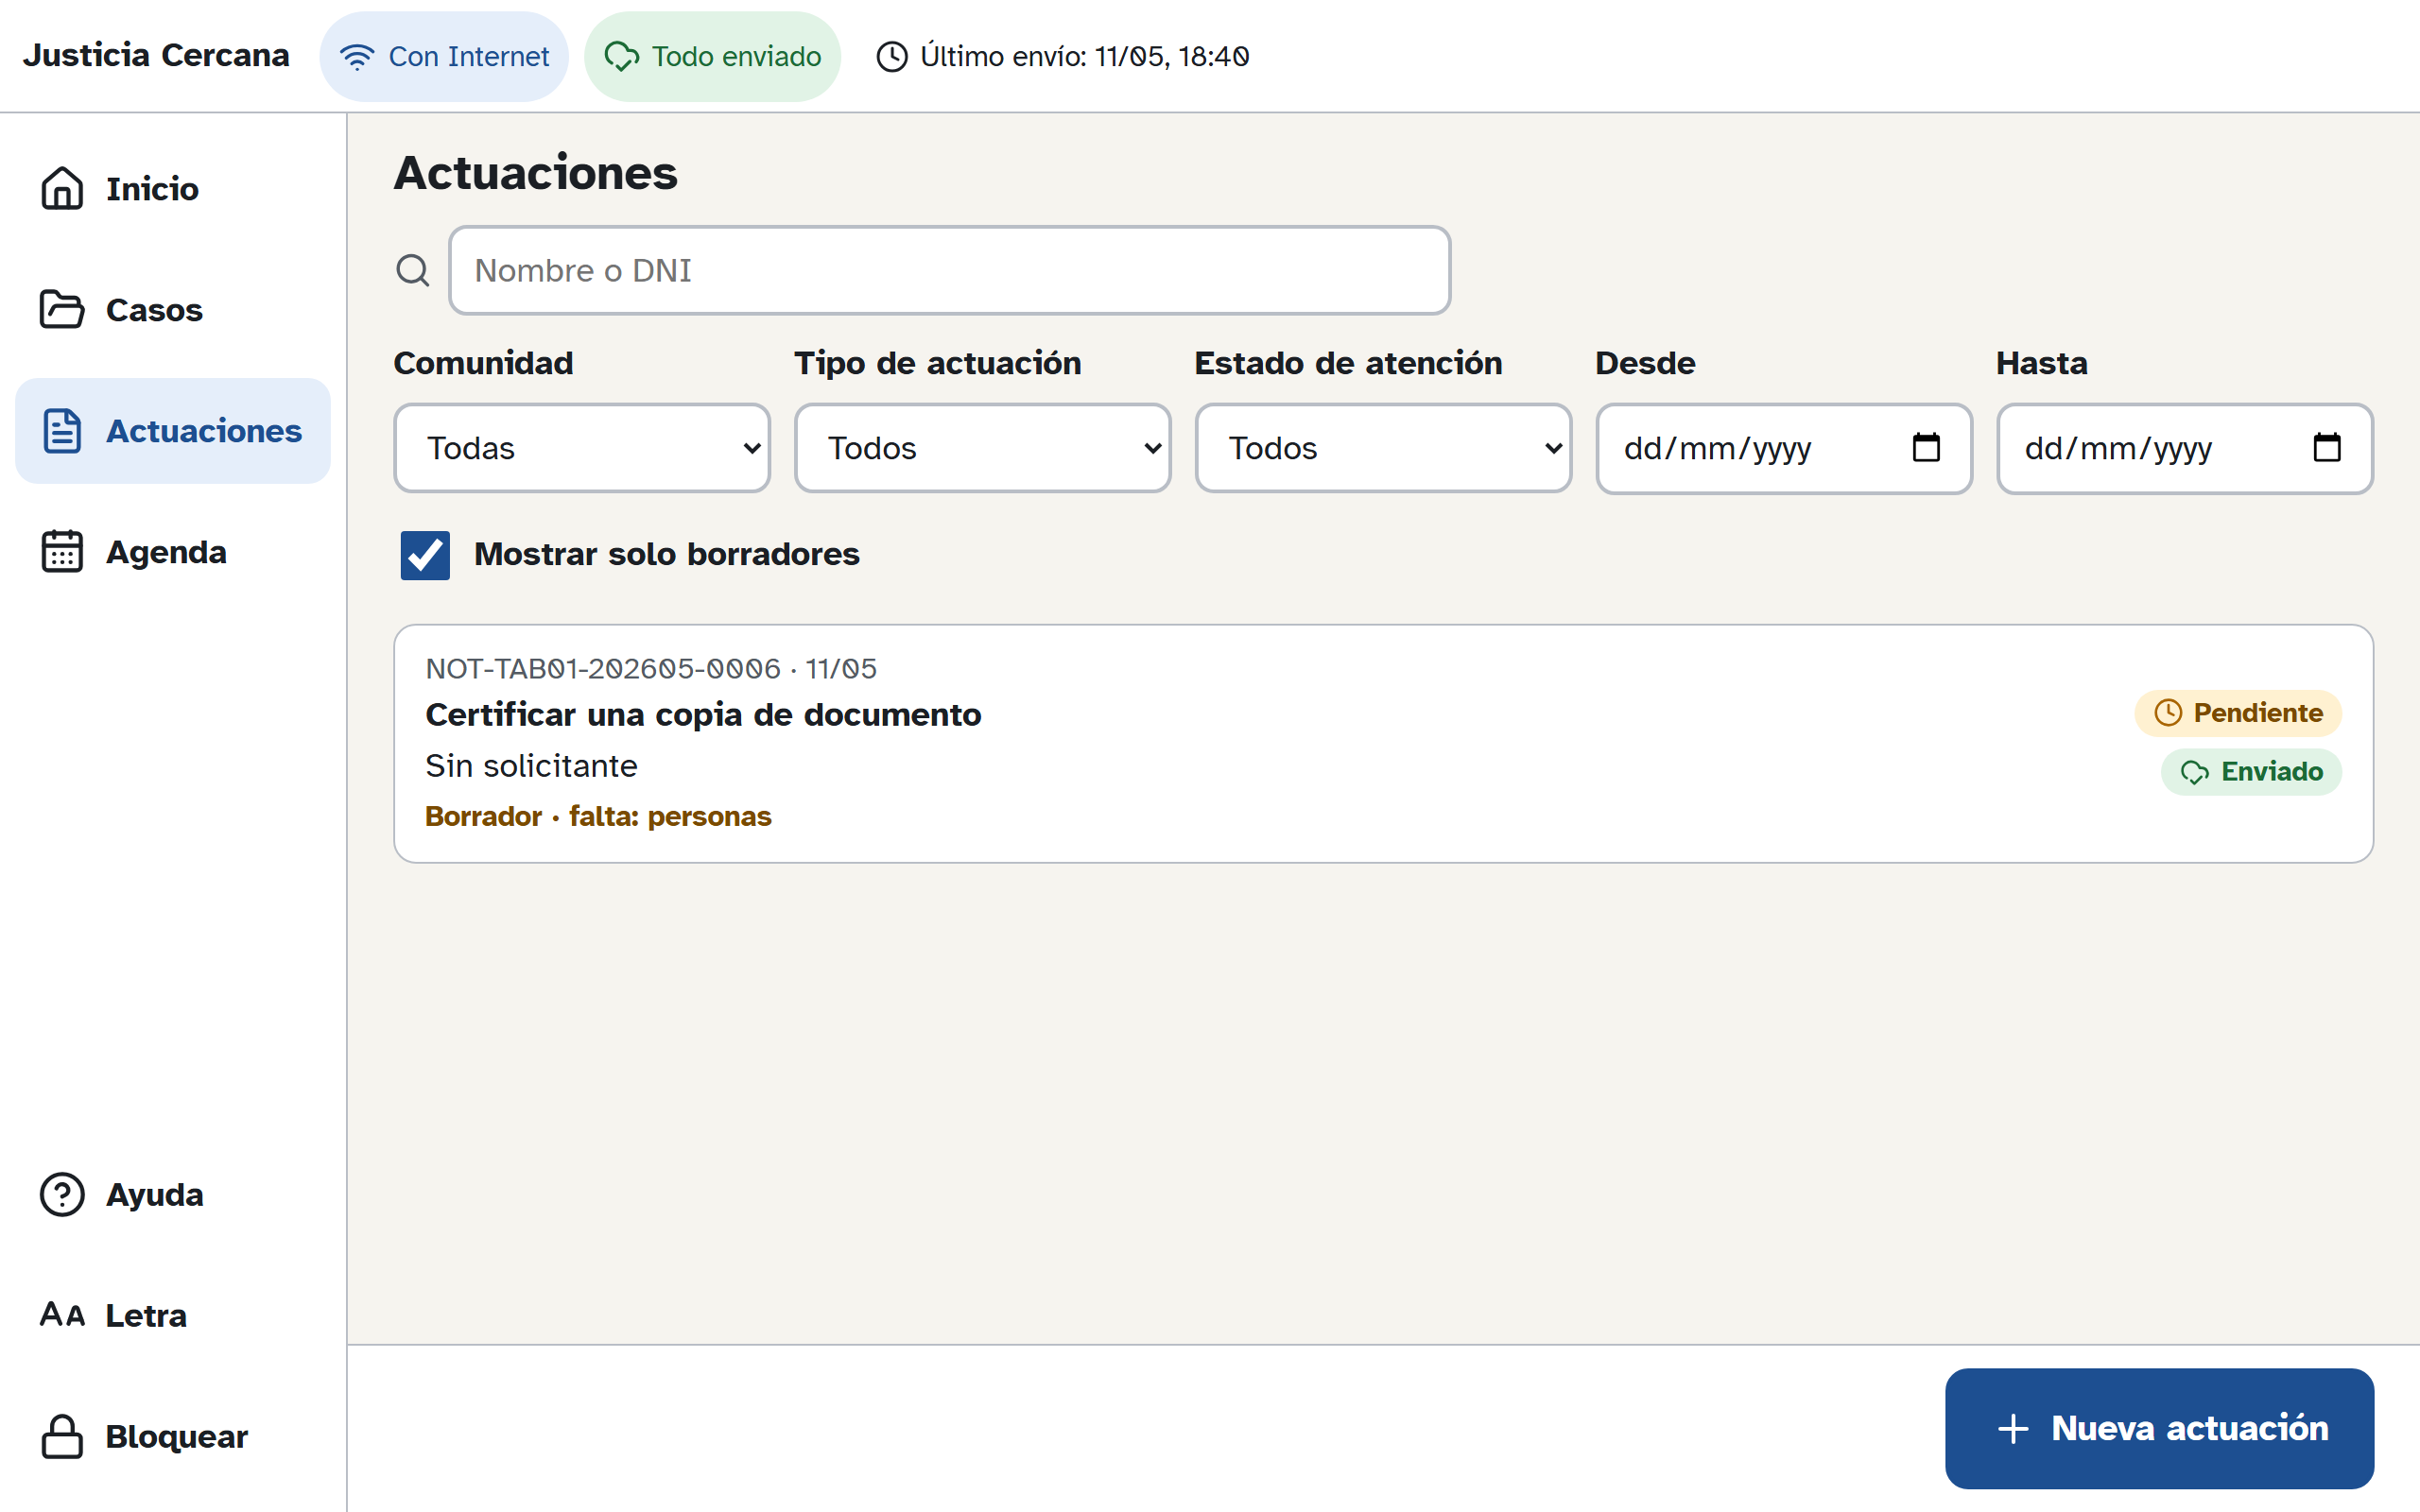
\includegraphics[width=\linewidth]{../../captures/G-09_borrador-actuaciones.png}\\[-2pt]{\footnotesize\raggedright\textbf{P-05.} ``Borrador · falta: personas'' y filtro de borradores (actuaciones) \emph{(Principios de diseño y heurísticas)}\par}\end{minipage}\par\vspace{8pt}\noindent
\begin{minipage}[t]{0.49\textwidth}\centering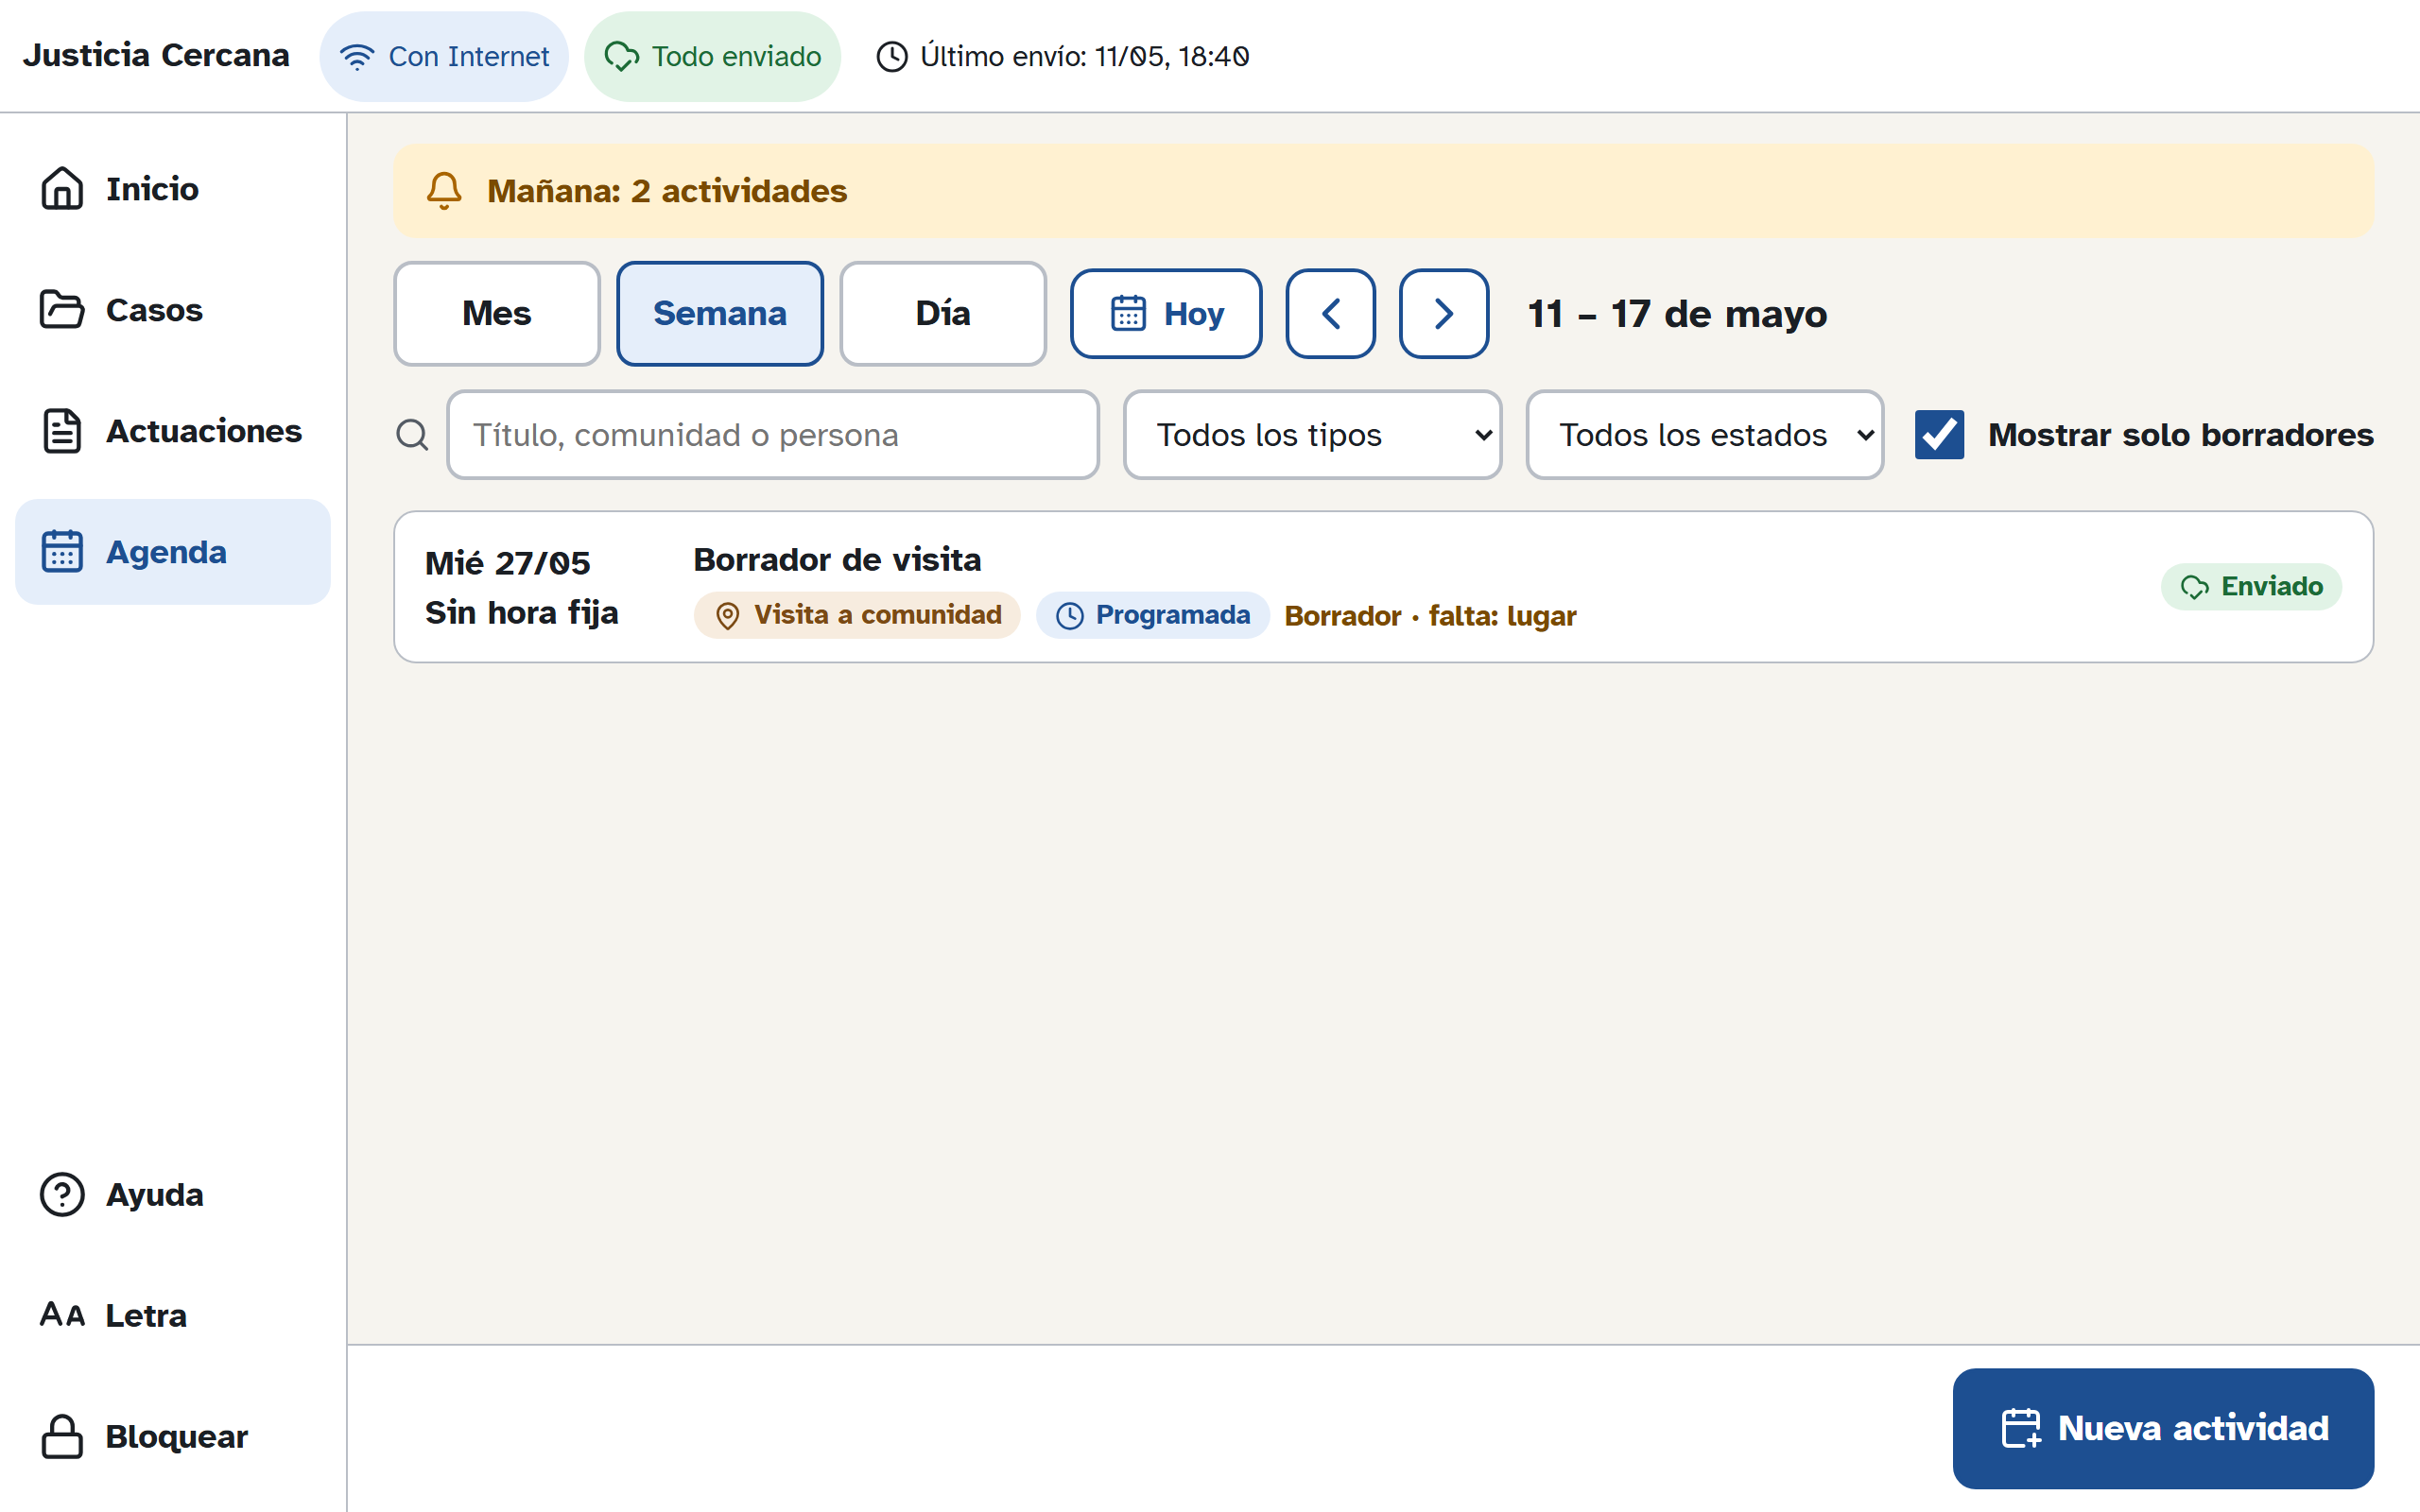
\includegraphics[width=\linewidth]{../../captures/G-10_borrador-agenda.png}\\[-2pt]{\footnotesize\raggedright\textbf{P-07.} ``Borrador · falta: lugar'' y filtro de borradores (agenda) \emph{(Principios de diseño y heurísticas)}\par}\end{minipage}\hfill
\begin{minipage}[t]{0.49\textwidth}\centering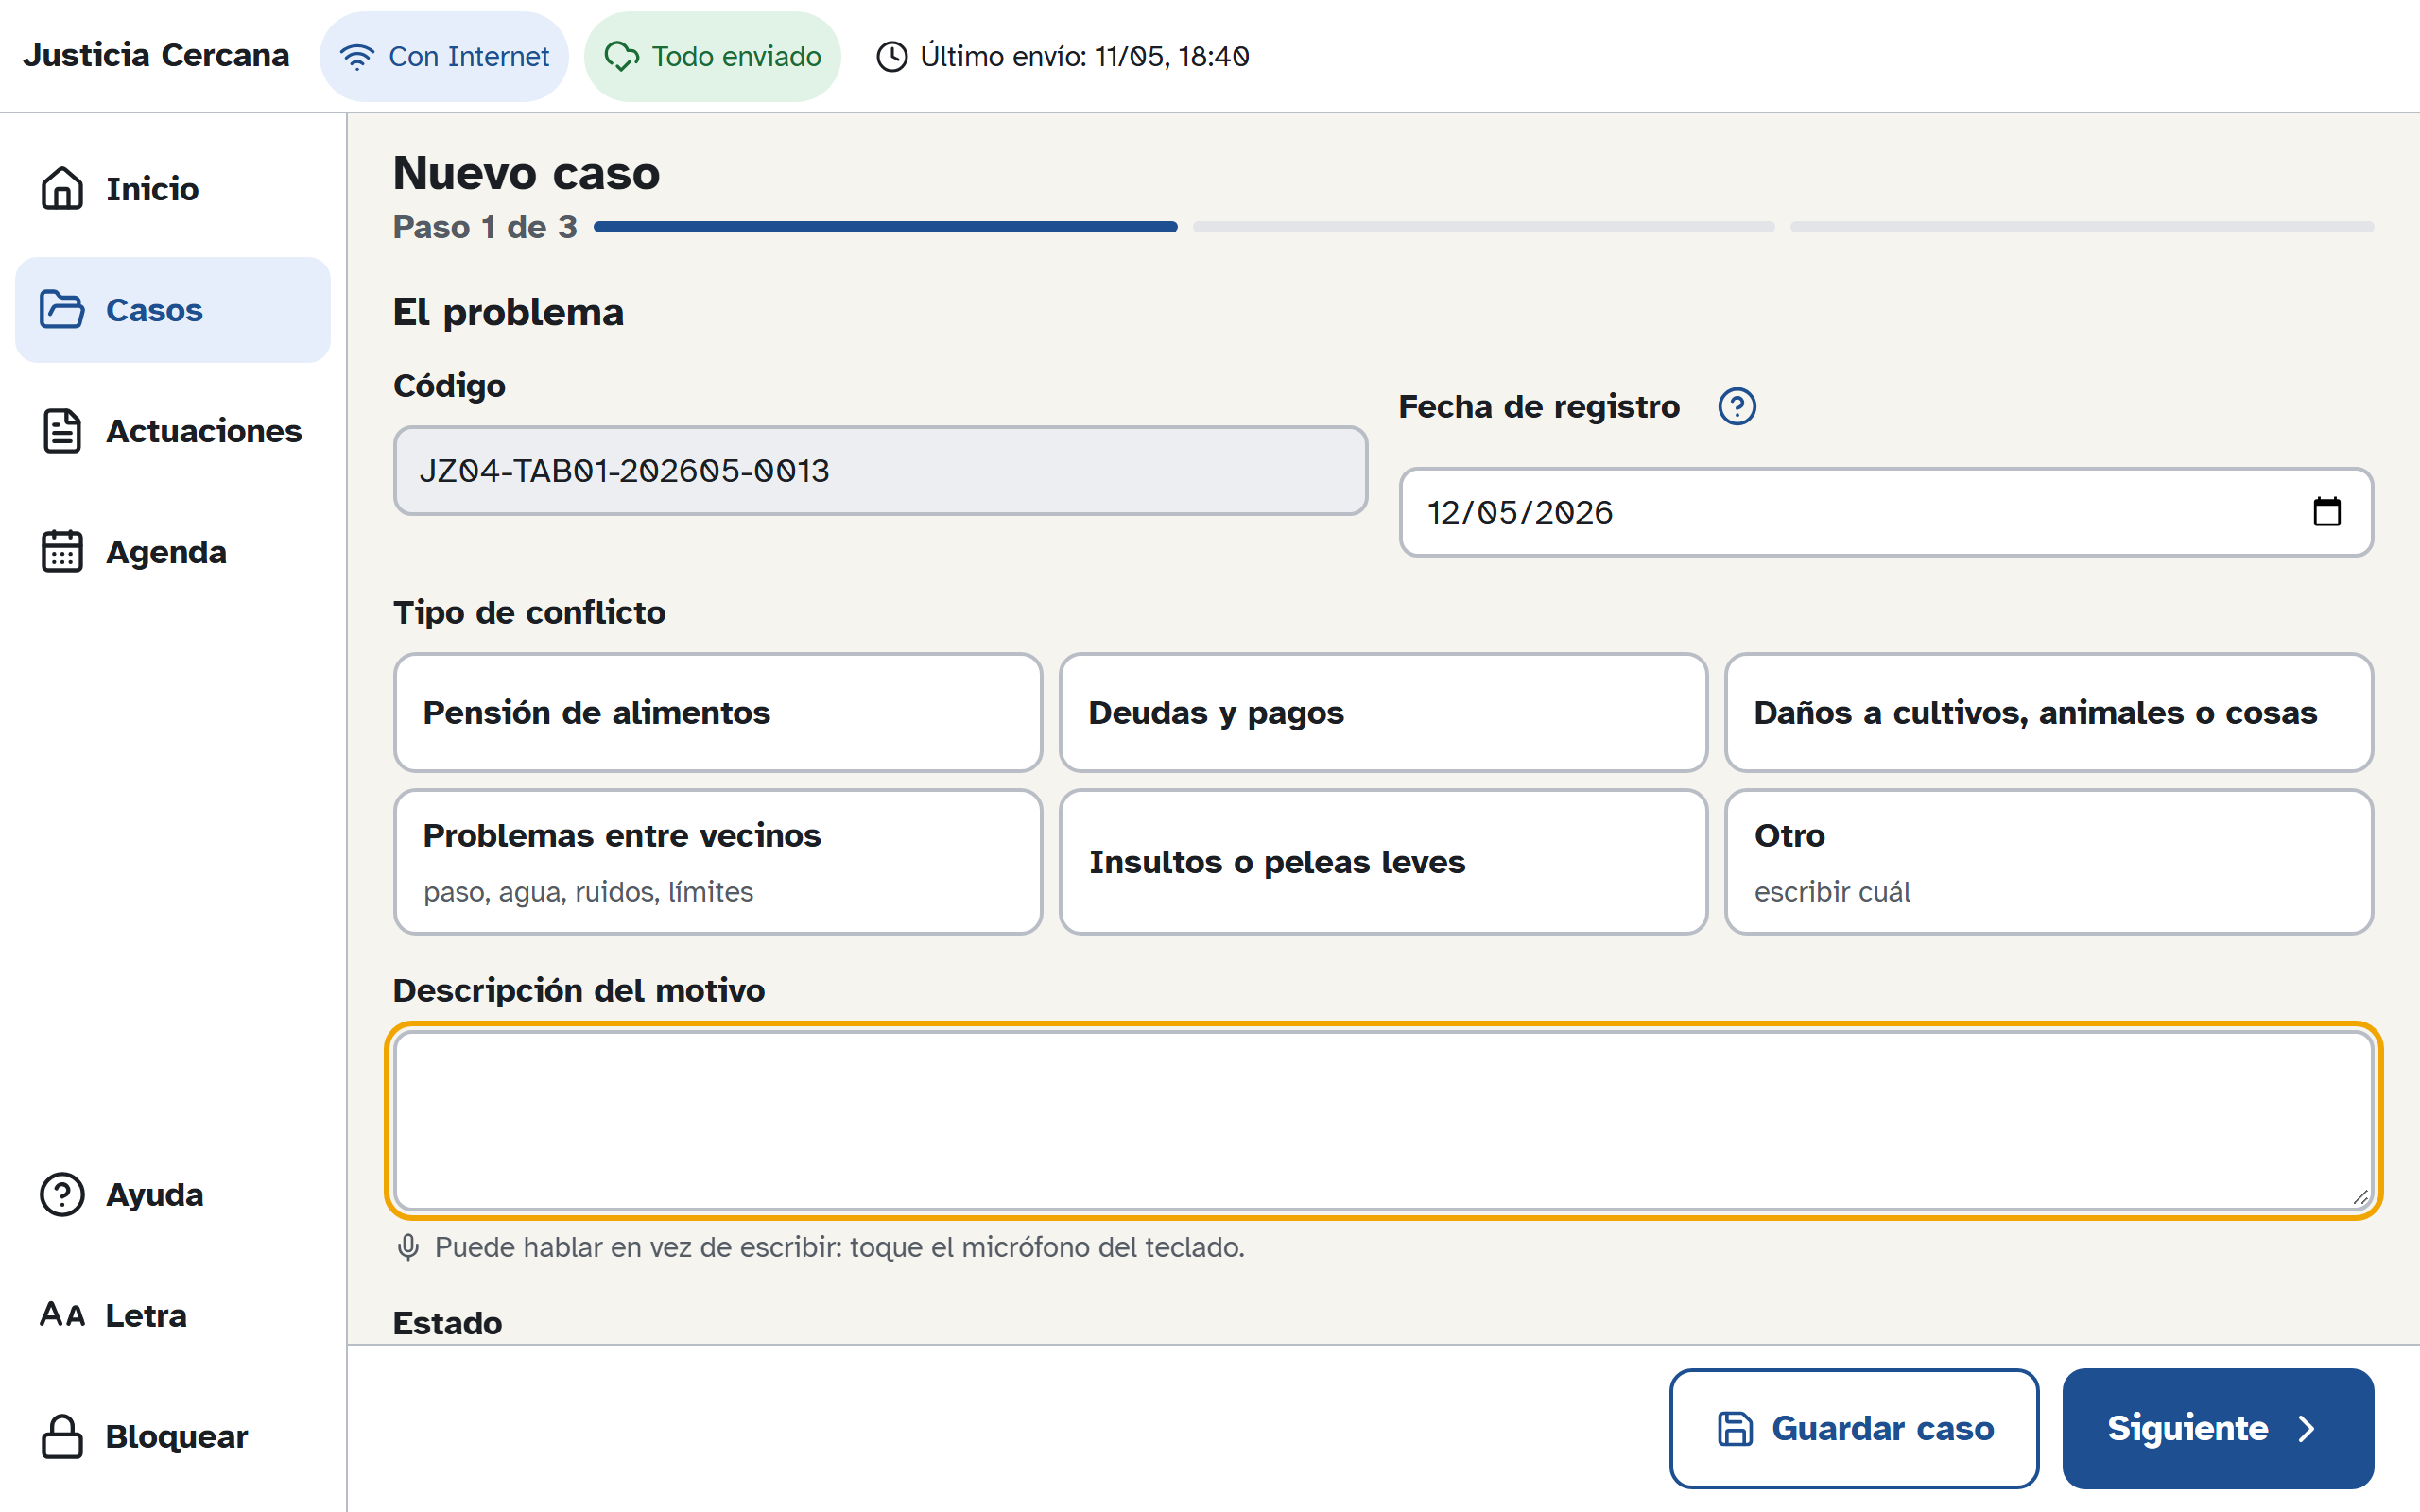
\includegraphics[width=\linewidth]{../../captures/G-11_ayuda-dictado.png}\\[-2pt]{\footnotesize\raggedright\textbf{P-03.} Ayuda de dictado del teclado bajo el campo largo (sin micrófono propio) \emph{(Factores humanos y dispositivo)}\par}\end{minipage}\par\vspace{8pt}\noindent
\begin{minipage}[t]{0.49\textwidth}\centering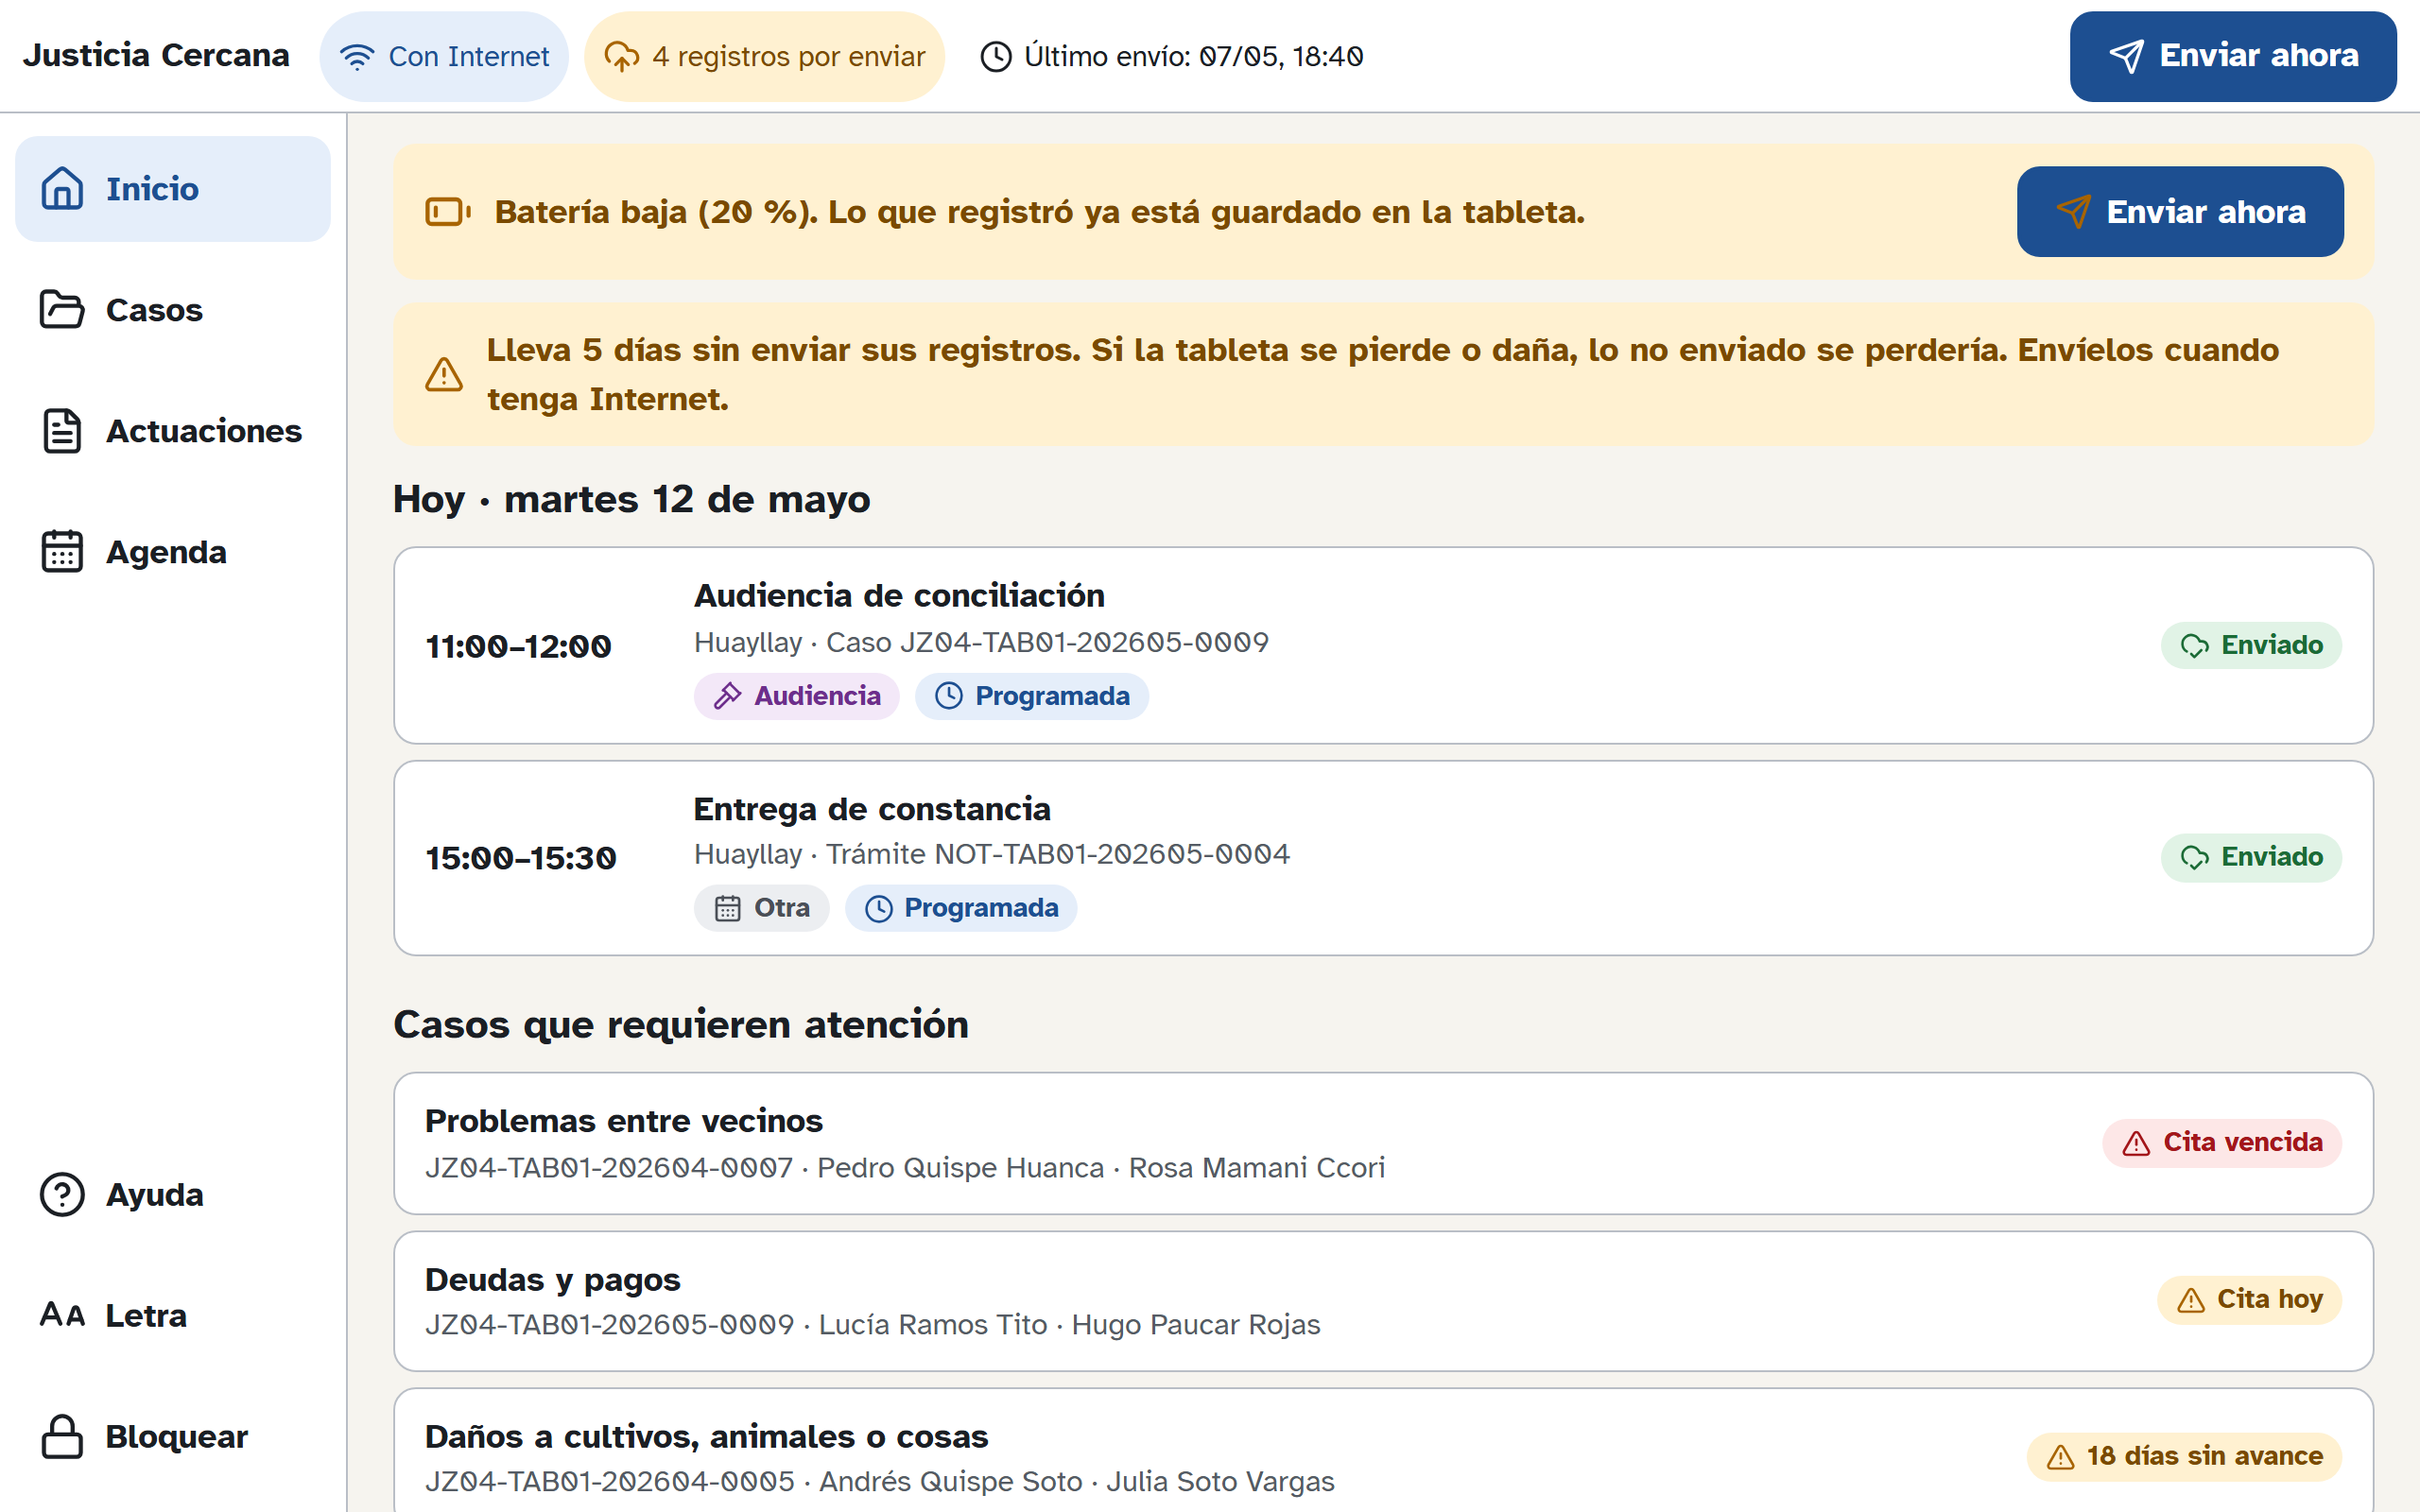
\includegraphics[width=\linewidth]{../../captures/G-12_bateria-20.png}\\[-2pt]{\footnotesize\raggedright\textbf{P-01.} Batería baja 20 \%: lo registrado ya está en la tableta; [Enviar ahora] \emph{(Factores humanos y dispositivo)}\par}\end{minipage}\hfill
\begin{minipage}[t]{0.49\textwidth}\centering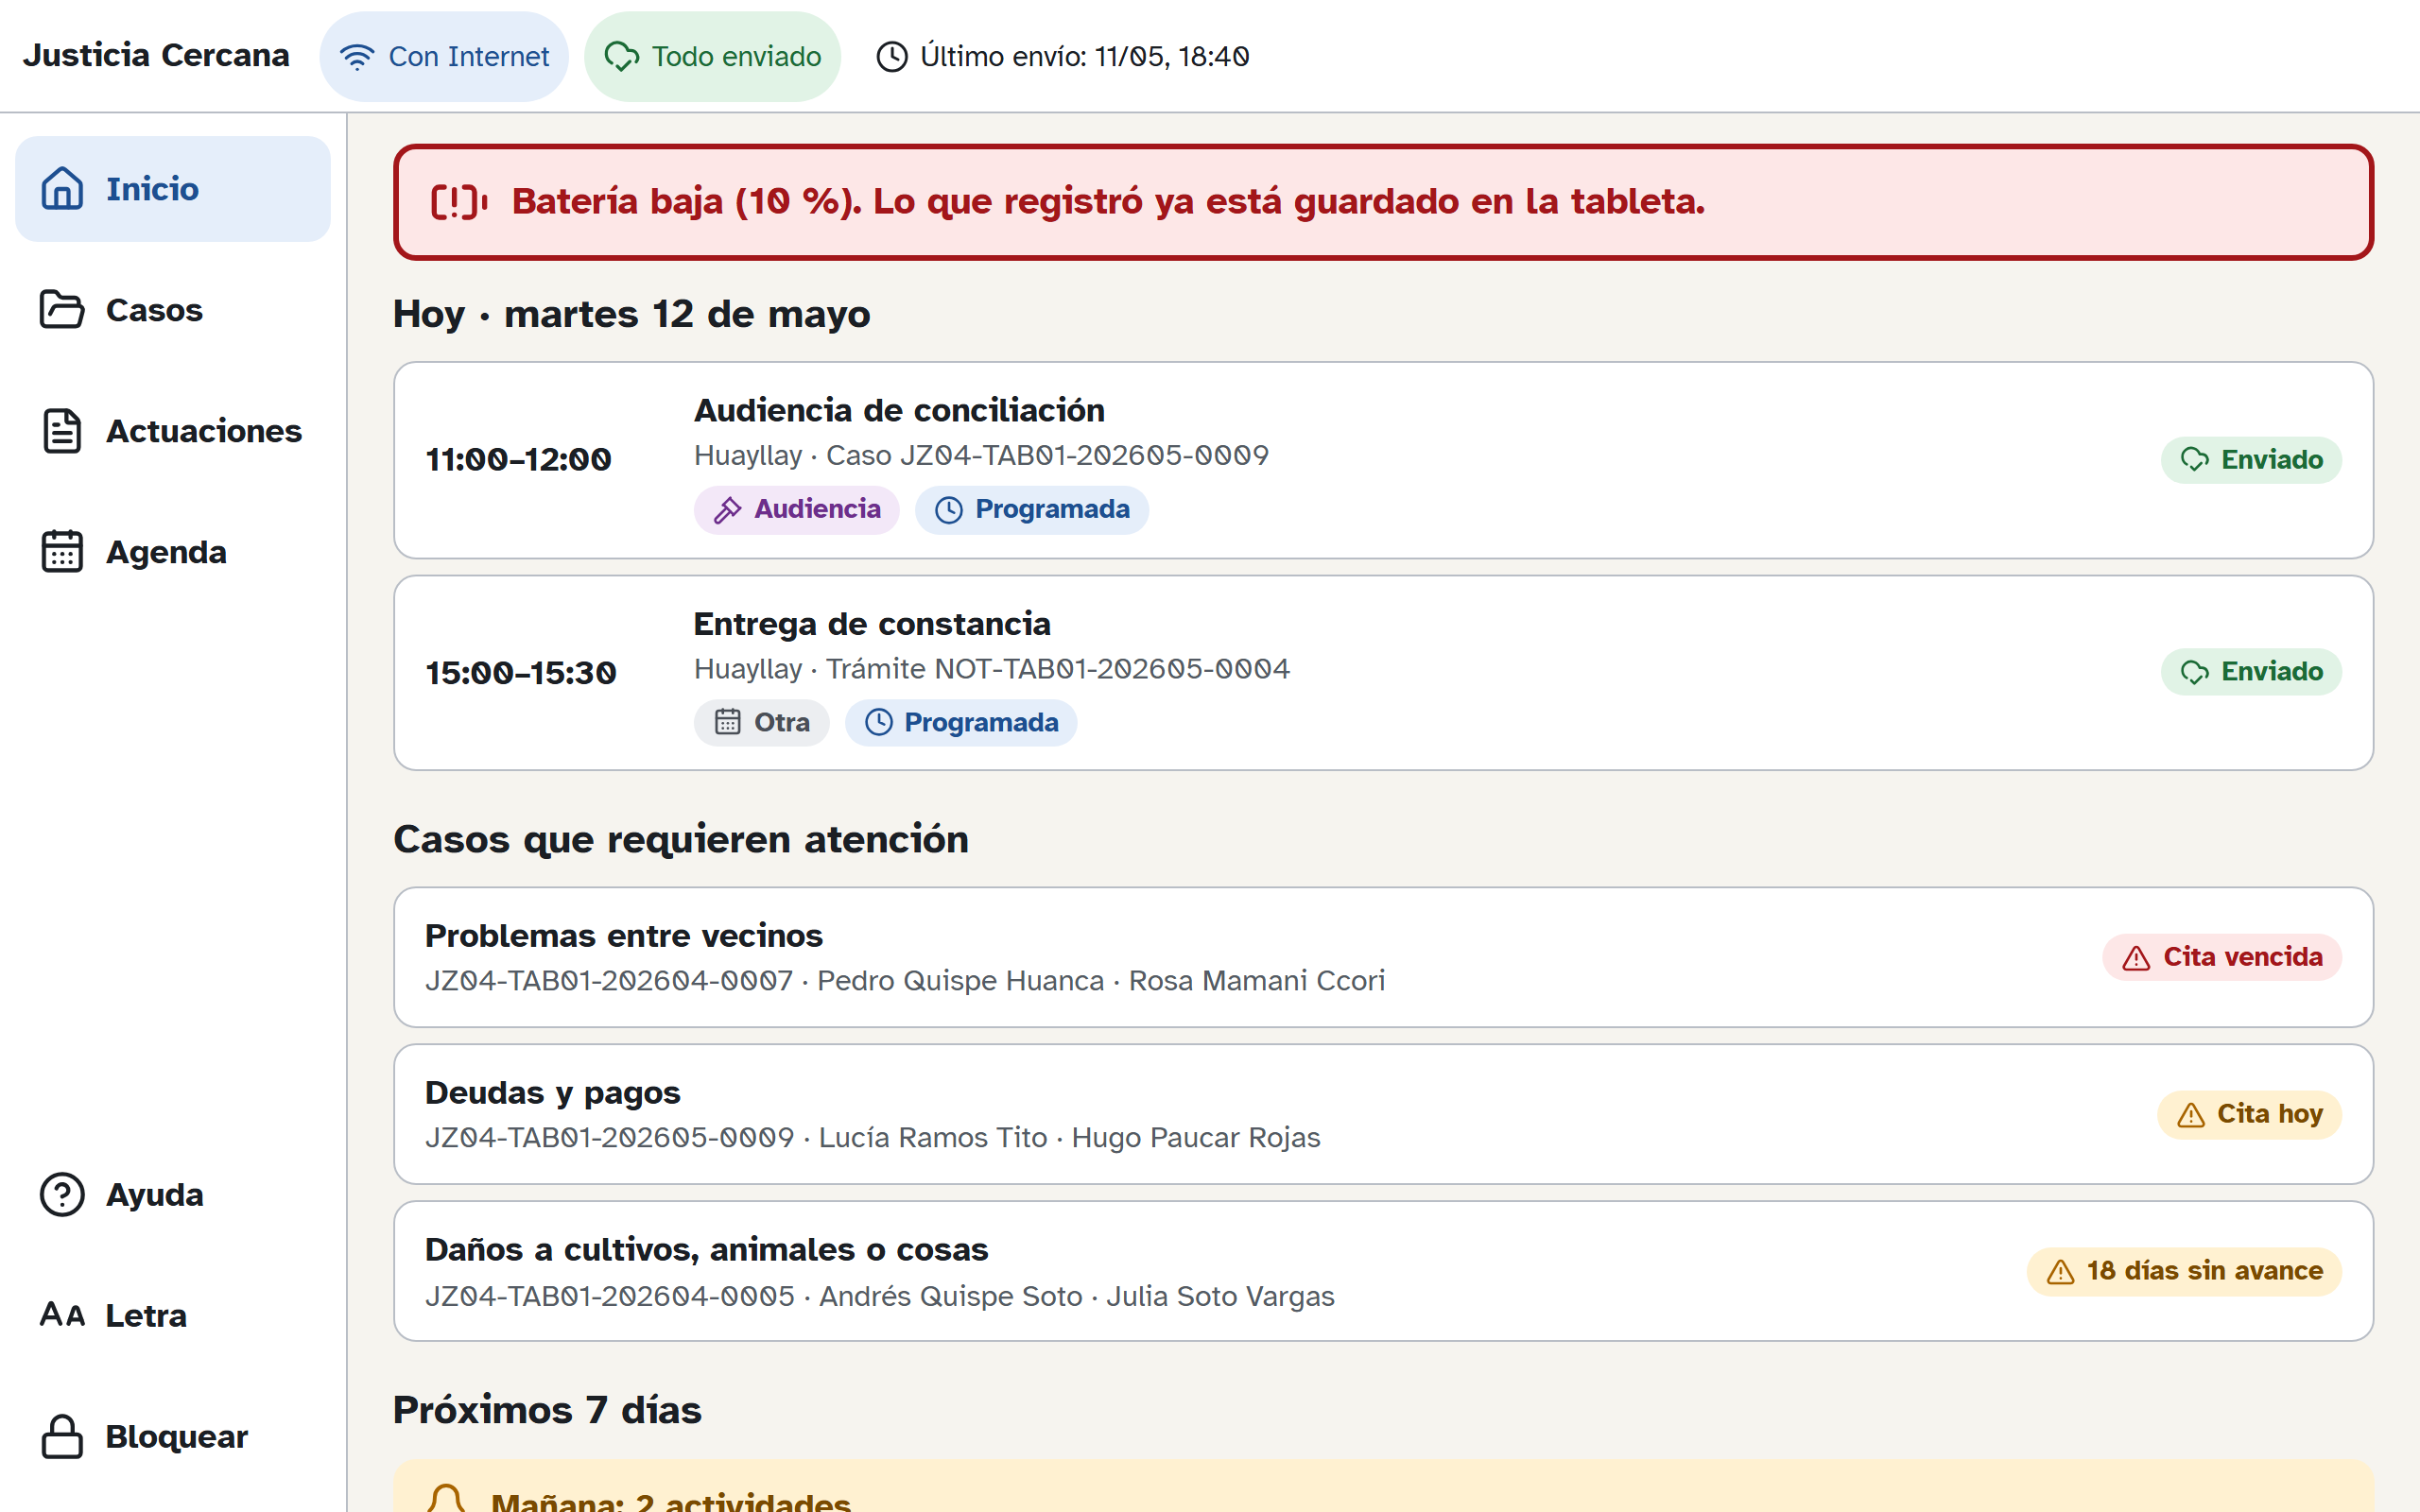
\includegraphics[width=\linewidth]{../../captures/G-13_bateria-10.png}\\[-2pt]{\footnotesize\raggedright\textbf{P-01.} Batería 10 \%: aviso más visible \emph{(Factores humanos y dispositivo)}\par}\end{minipage}\par\vspace{8pt}\noindent
\begin{minipage}[t]{0.49\textwidth}\centering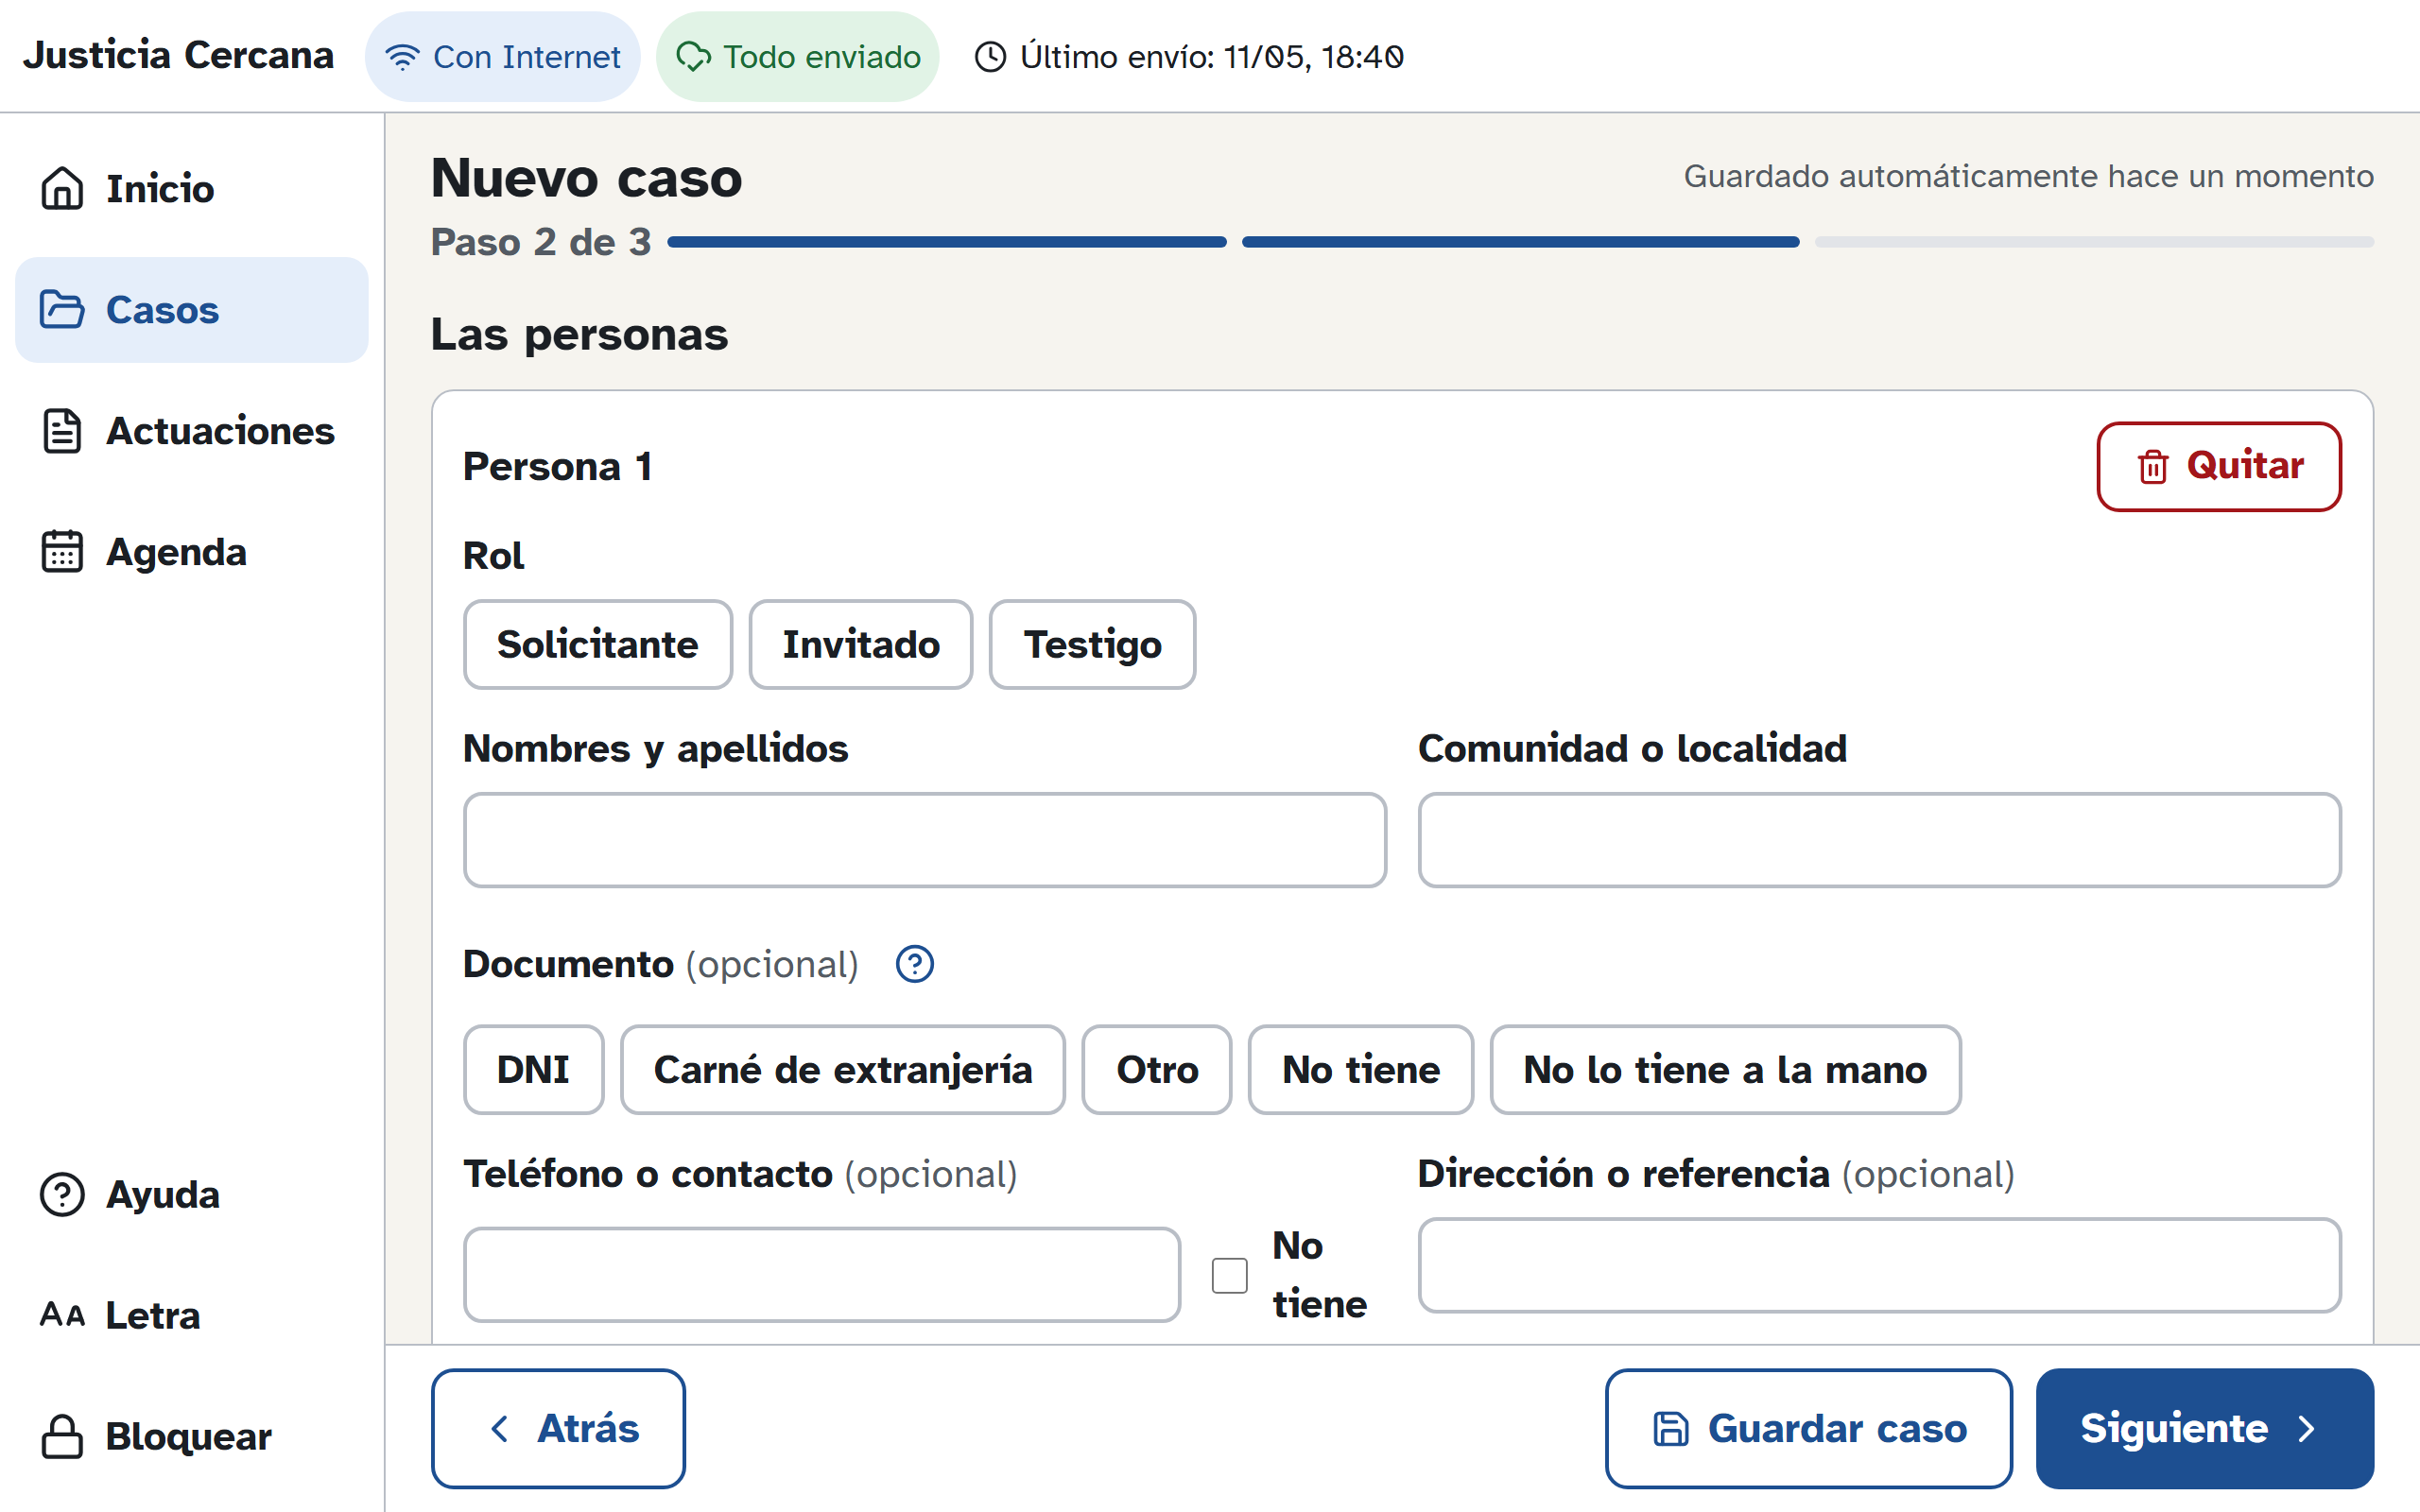
\includegraphics[width=\linewidth]{../../captures/G-14_letra-grande-formulario.png}\\[-2pt]{\footnotesize\raggedright\textbf{P-03.} Formulario en letra Grande (21 px) sin romper el diseño \emph{(Factores humanos y dispositivo)}\par}\end{minipage}\hfill
\begin{minipage}[t]{0.49\textwidth}\centering
\includegraphics[width=\linewidth]{../../captures/G-15_gire-la-tableta.png}\\[-2pt]{\footnotesize\raggedright\textbf{Global.} ``Gire la tableta para usarla de lado'' en vertical 800×1280 \emph{(Factores humanos y dispositivo)}\par}\end{minipage}\par\vspace{8pt}\noindent
\begin{minipage}[t]{0.49\textwidth}\centering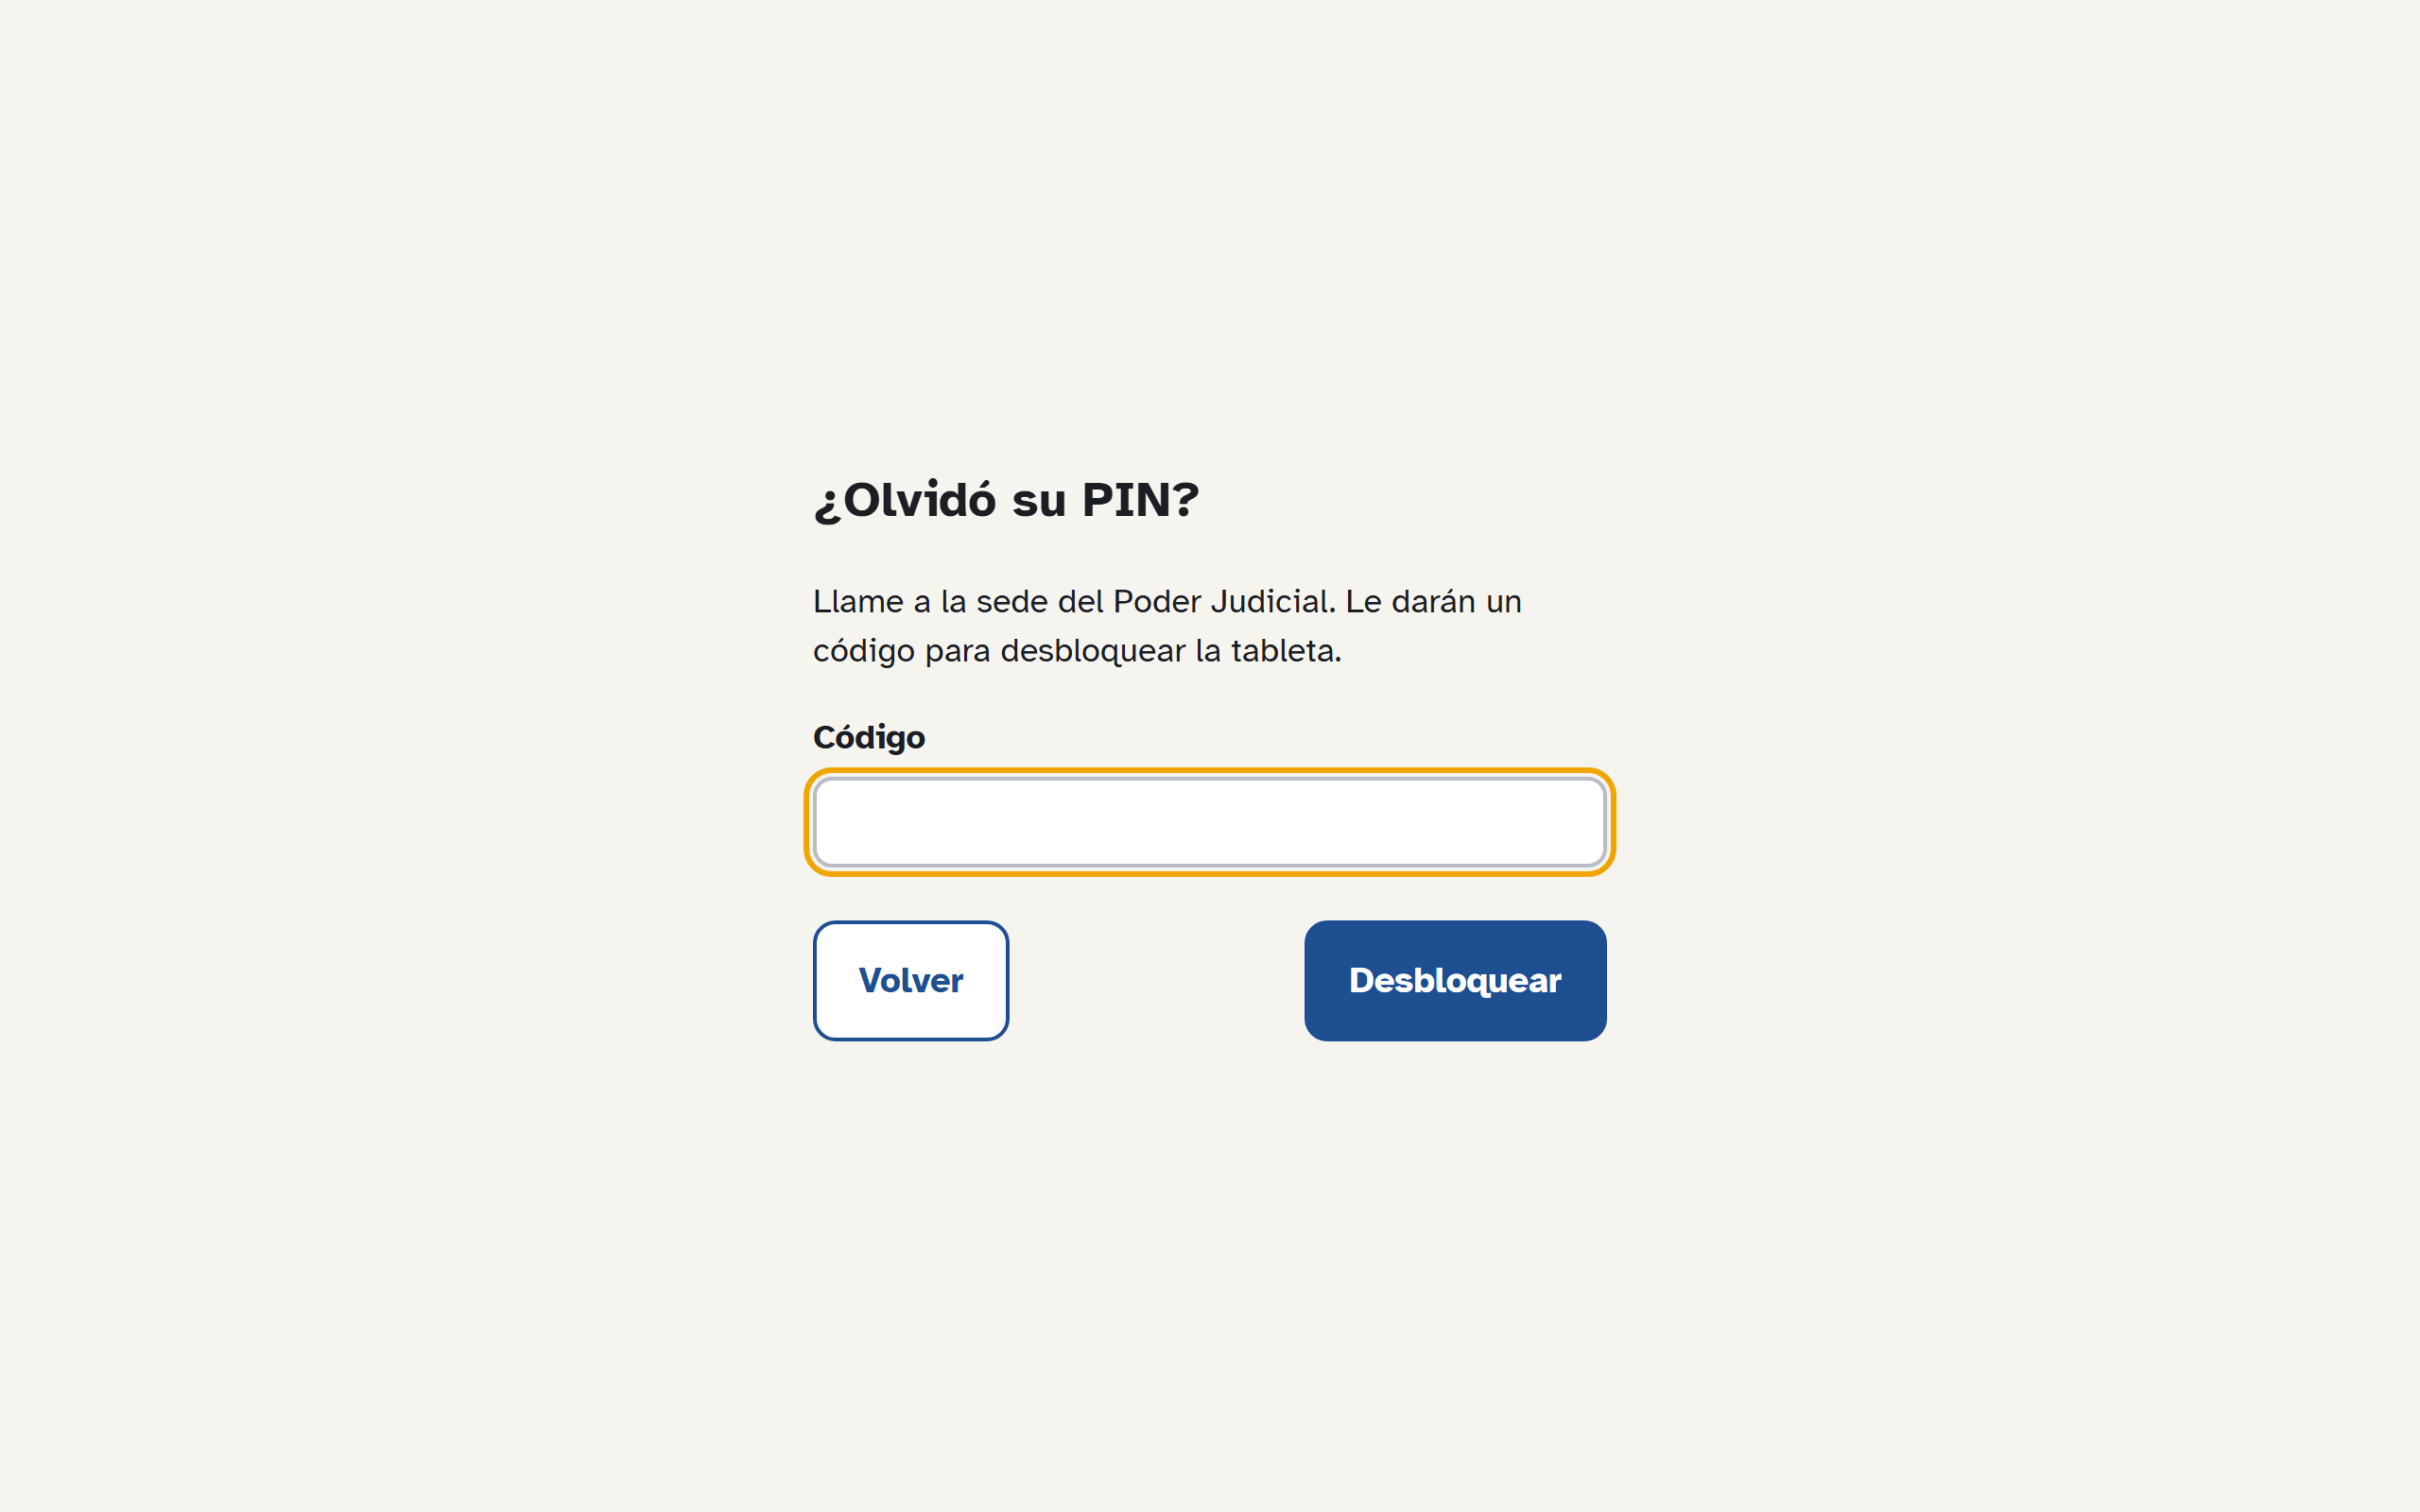
\includegraphics[width=\linewidth]{../../captures/P-00_olvido-pin.png}\\[-2pt]{\footnotesize\raggedright\textbf{P-00.} ``¿Olvidó su PIN?'' con explicación y campo para el código de la sede \emph{(Principios de diseño y heurísticas)}\par}\end{minipage}\hfill
\begin{minipage}[t]{0.49\textwidth}\centering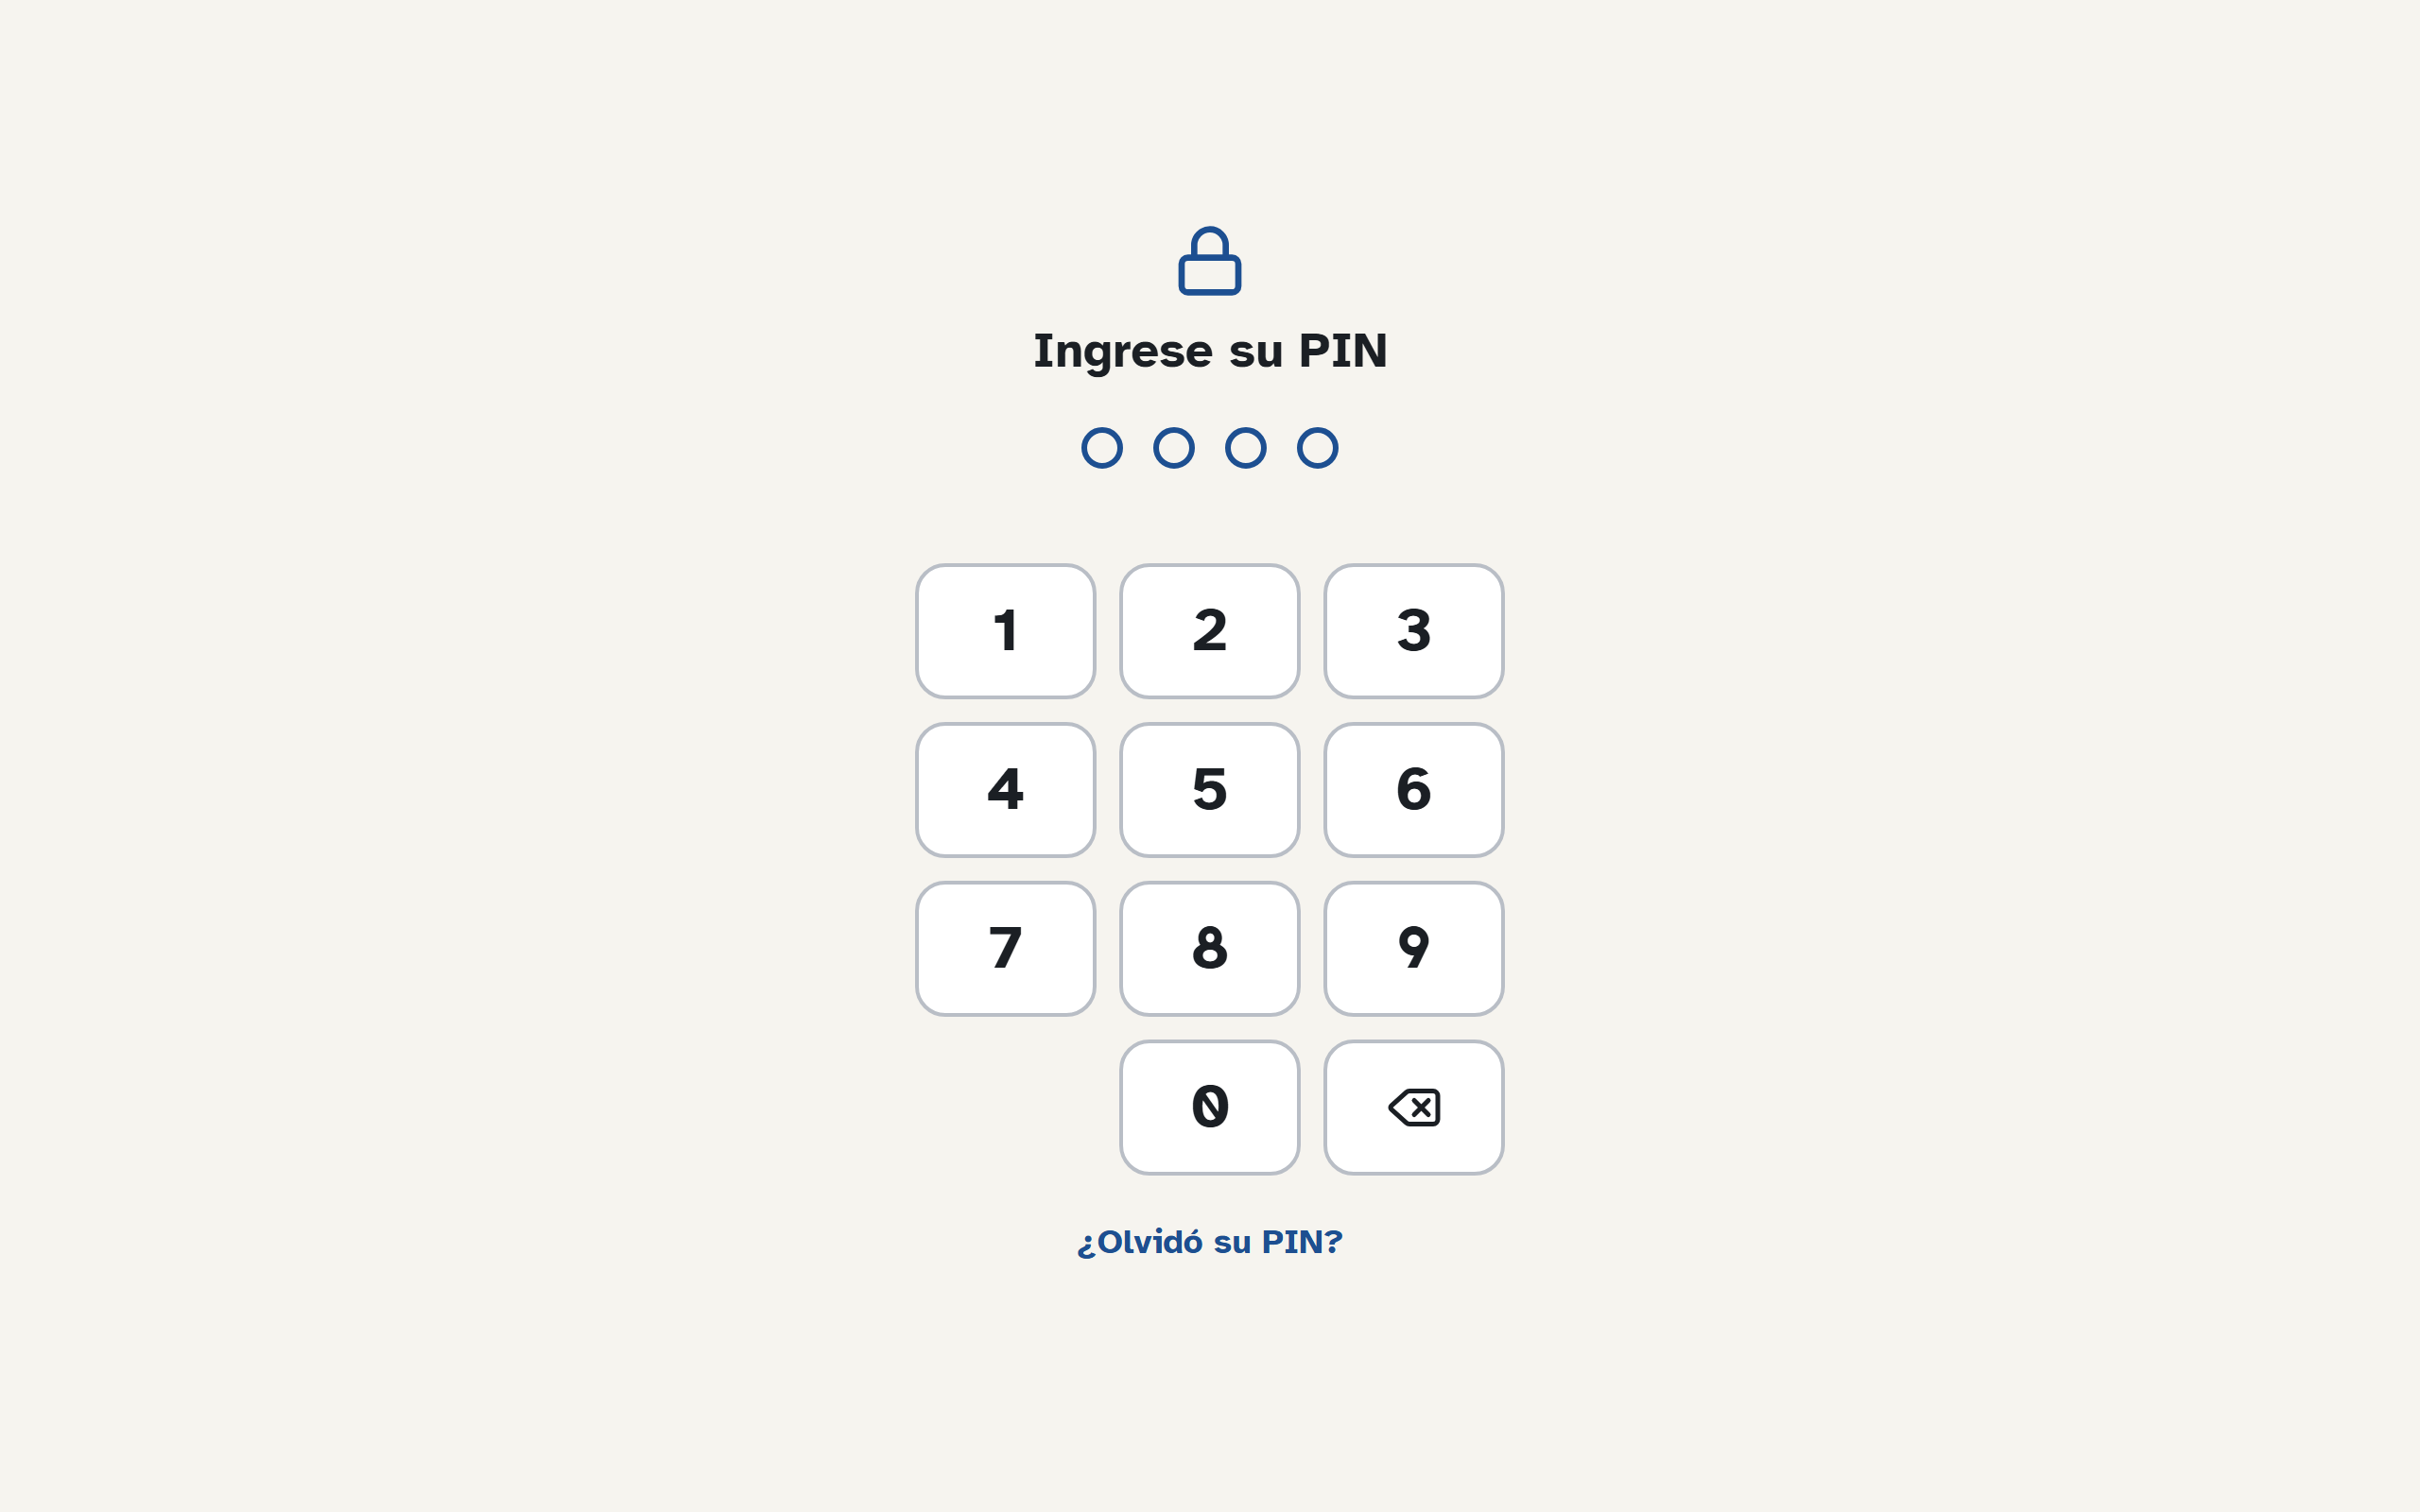
\includegraphics[width=\linewidth]{../../captures/P-00_pin.png}\\[-2pt]{\footnotesize\raggedright\textbf{P-00.} Ingreso con PIN: teclado numérico grande, sin patrón gestual \emph{(Factores humanos y dispositivo)}\par}\end{minipage}\par\vspace{8pt}\noindent
\begin{minipage}[t]{0.49\textwidth}\centering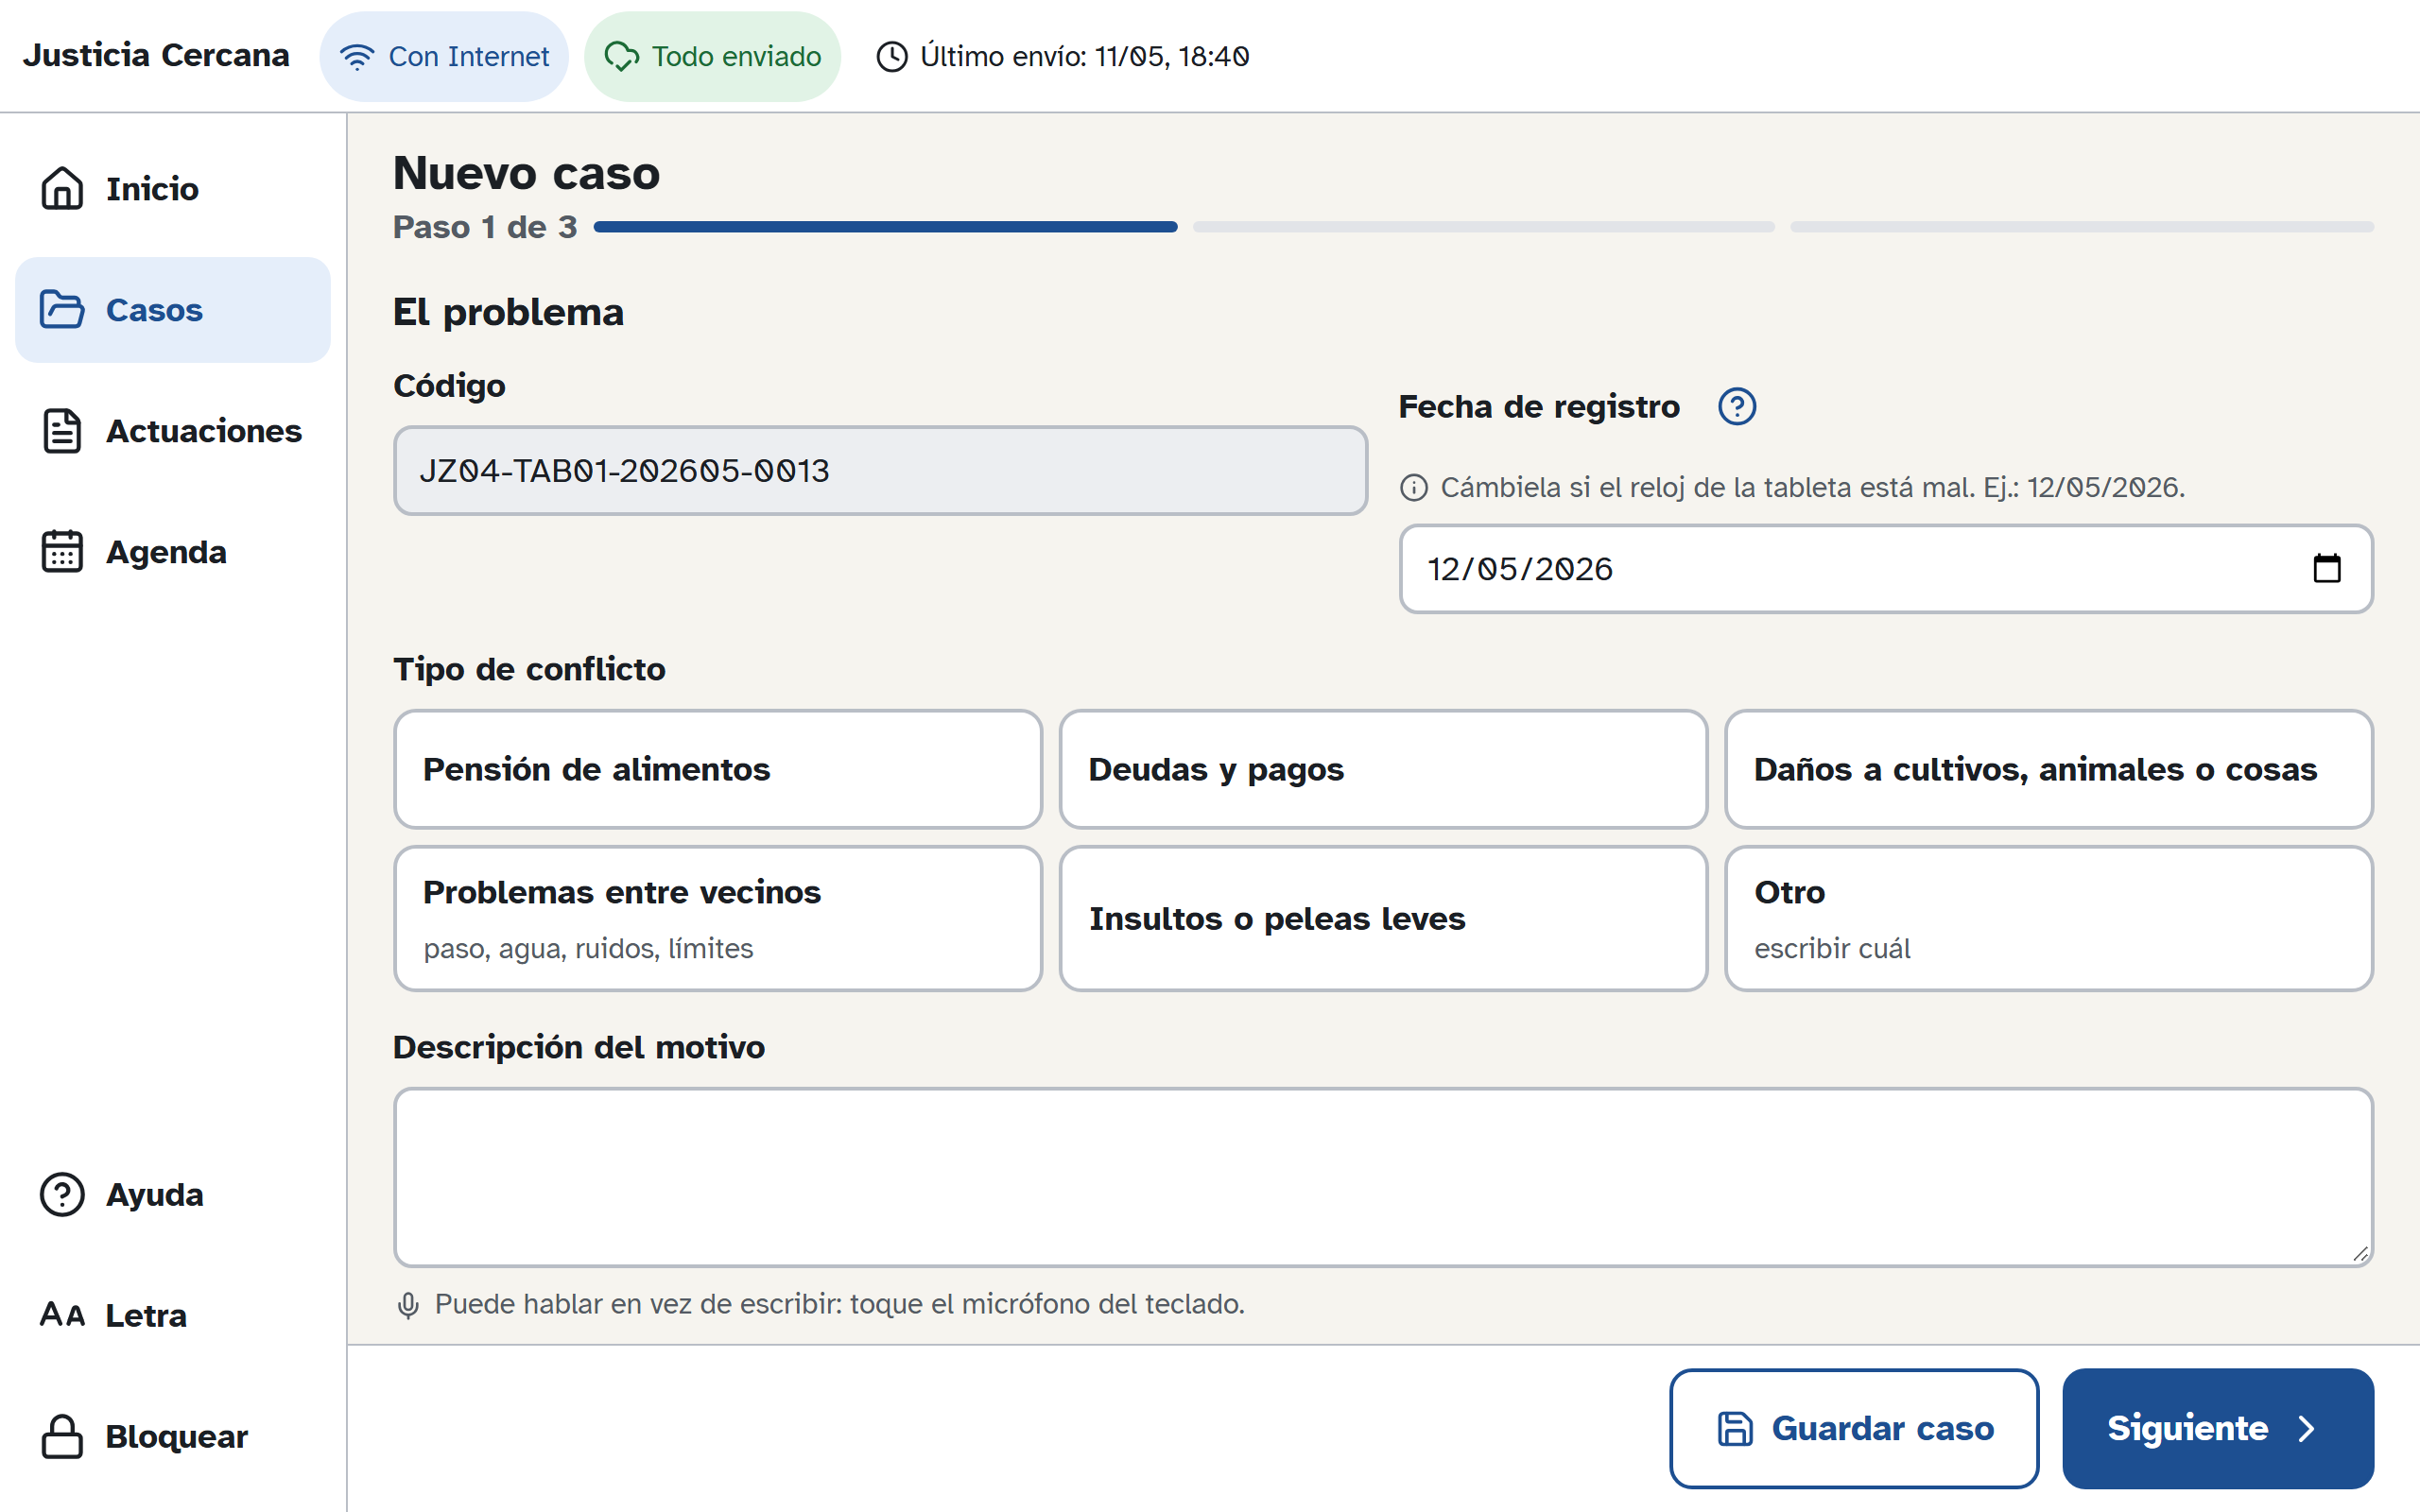
\includegraphics[width=\linewidth]{../../captures/P-00b_ayuda-por-campo.png}\\[-2pt]{\footnotesize\raggedright\textbf{P-00b.} Ayuda por campo (ícono help-circle): una línea con un ejemplo \emph{(Principios de diseño y heurísticas)}\par}\end{minipage}\hfill
\begin{minipage}[t]{0.49\textwidth}\centering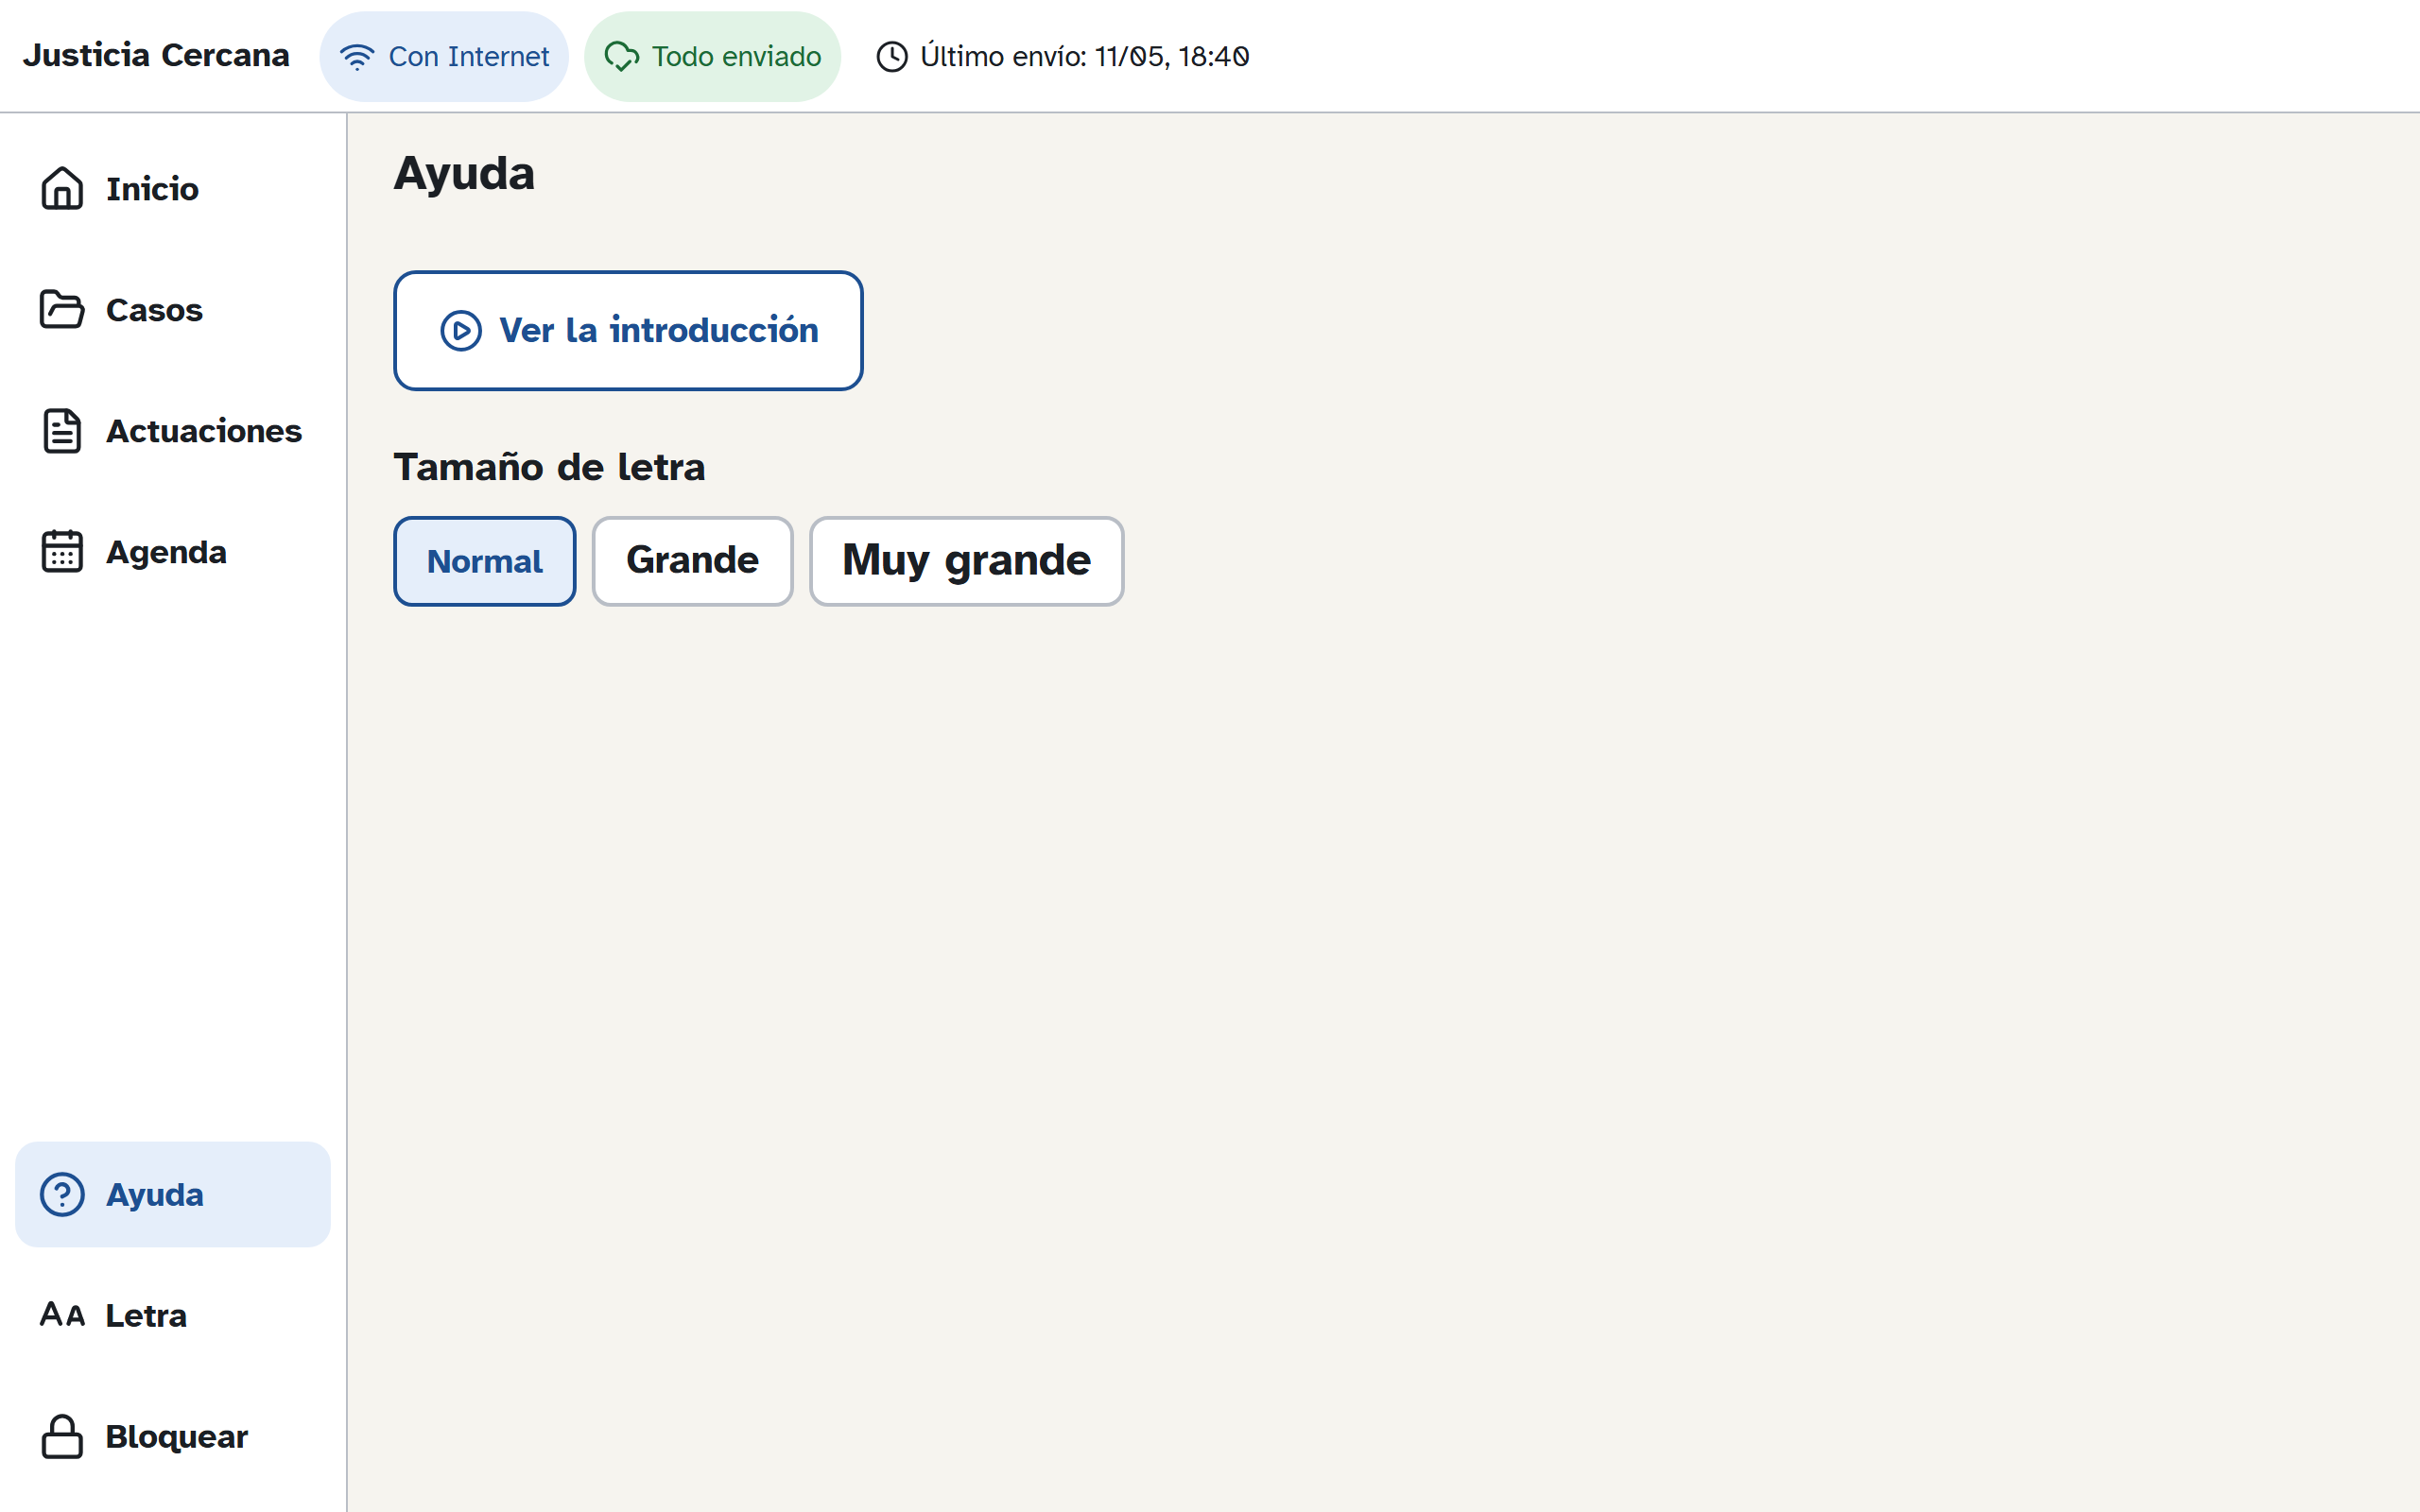
\includegraphics[width=\linewidth]{../../captures/P-00b_ayuda.png}\\[-2pt]{\footnotesize\raggedright\textbf{P-00b.} Ayuda: ver la introducción y tamaño de letra \emph{(Principios de diseño y heurísticas)}\par}\end{minipage}\par\vspace{8pt}\noindent
\begin{minipage}[t]{0.49\textwidth}\centering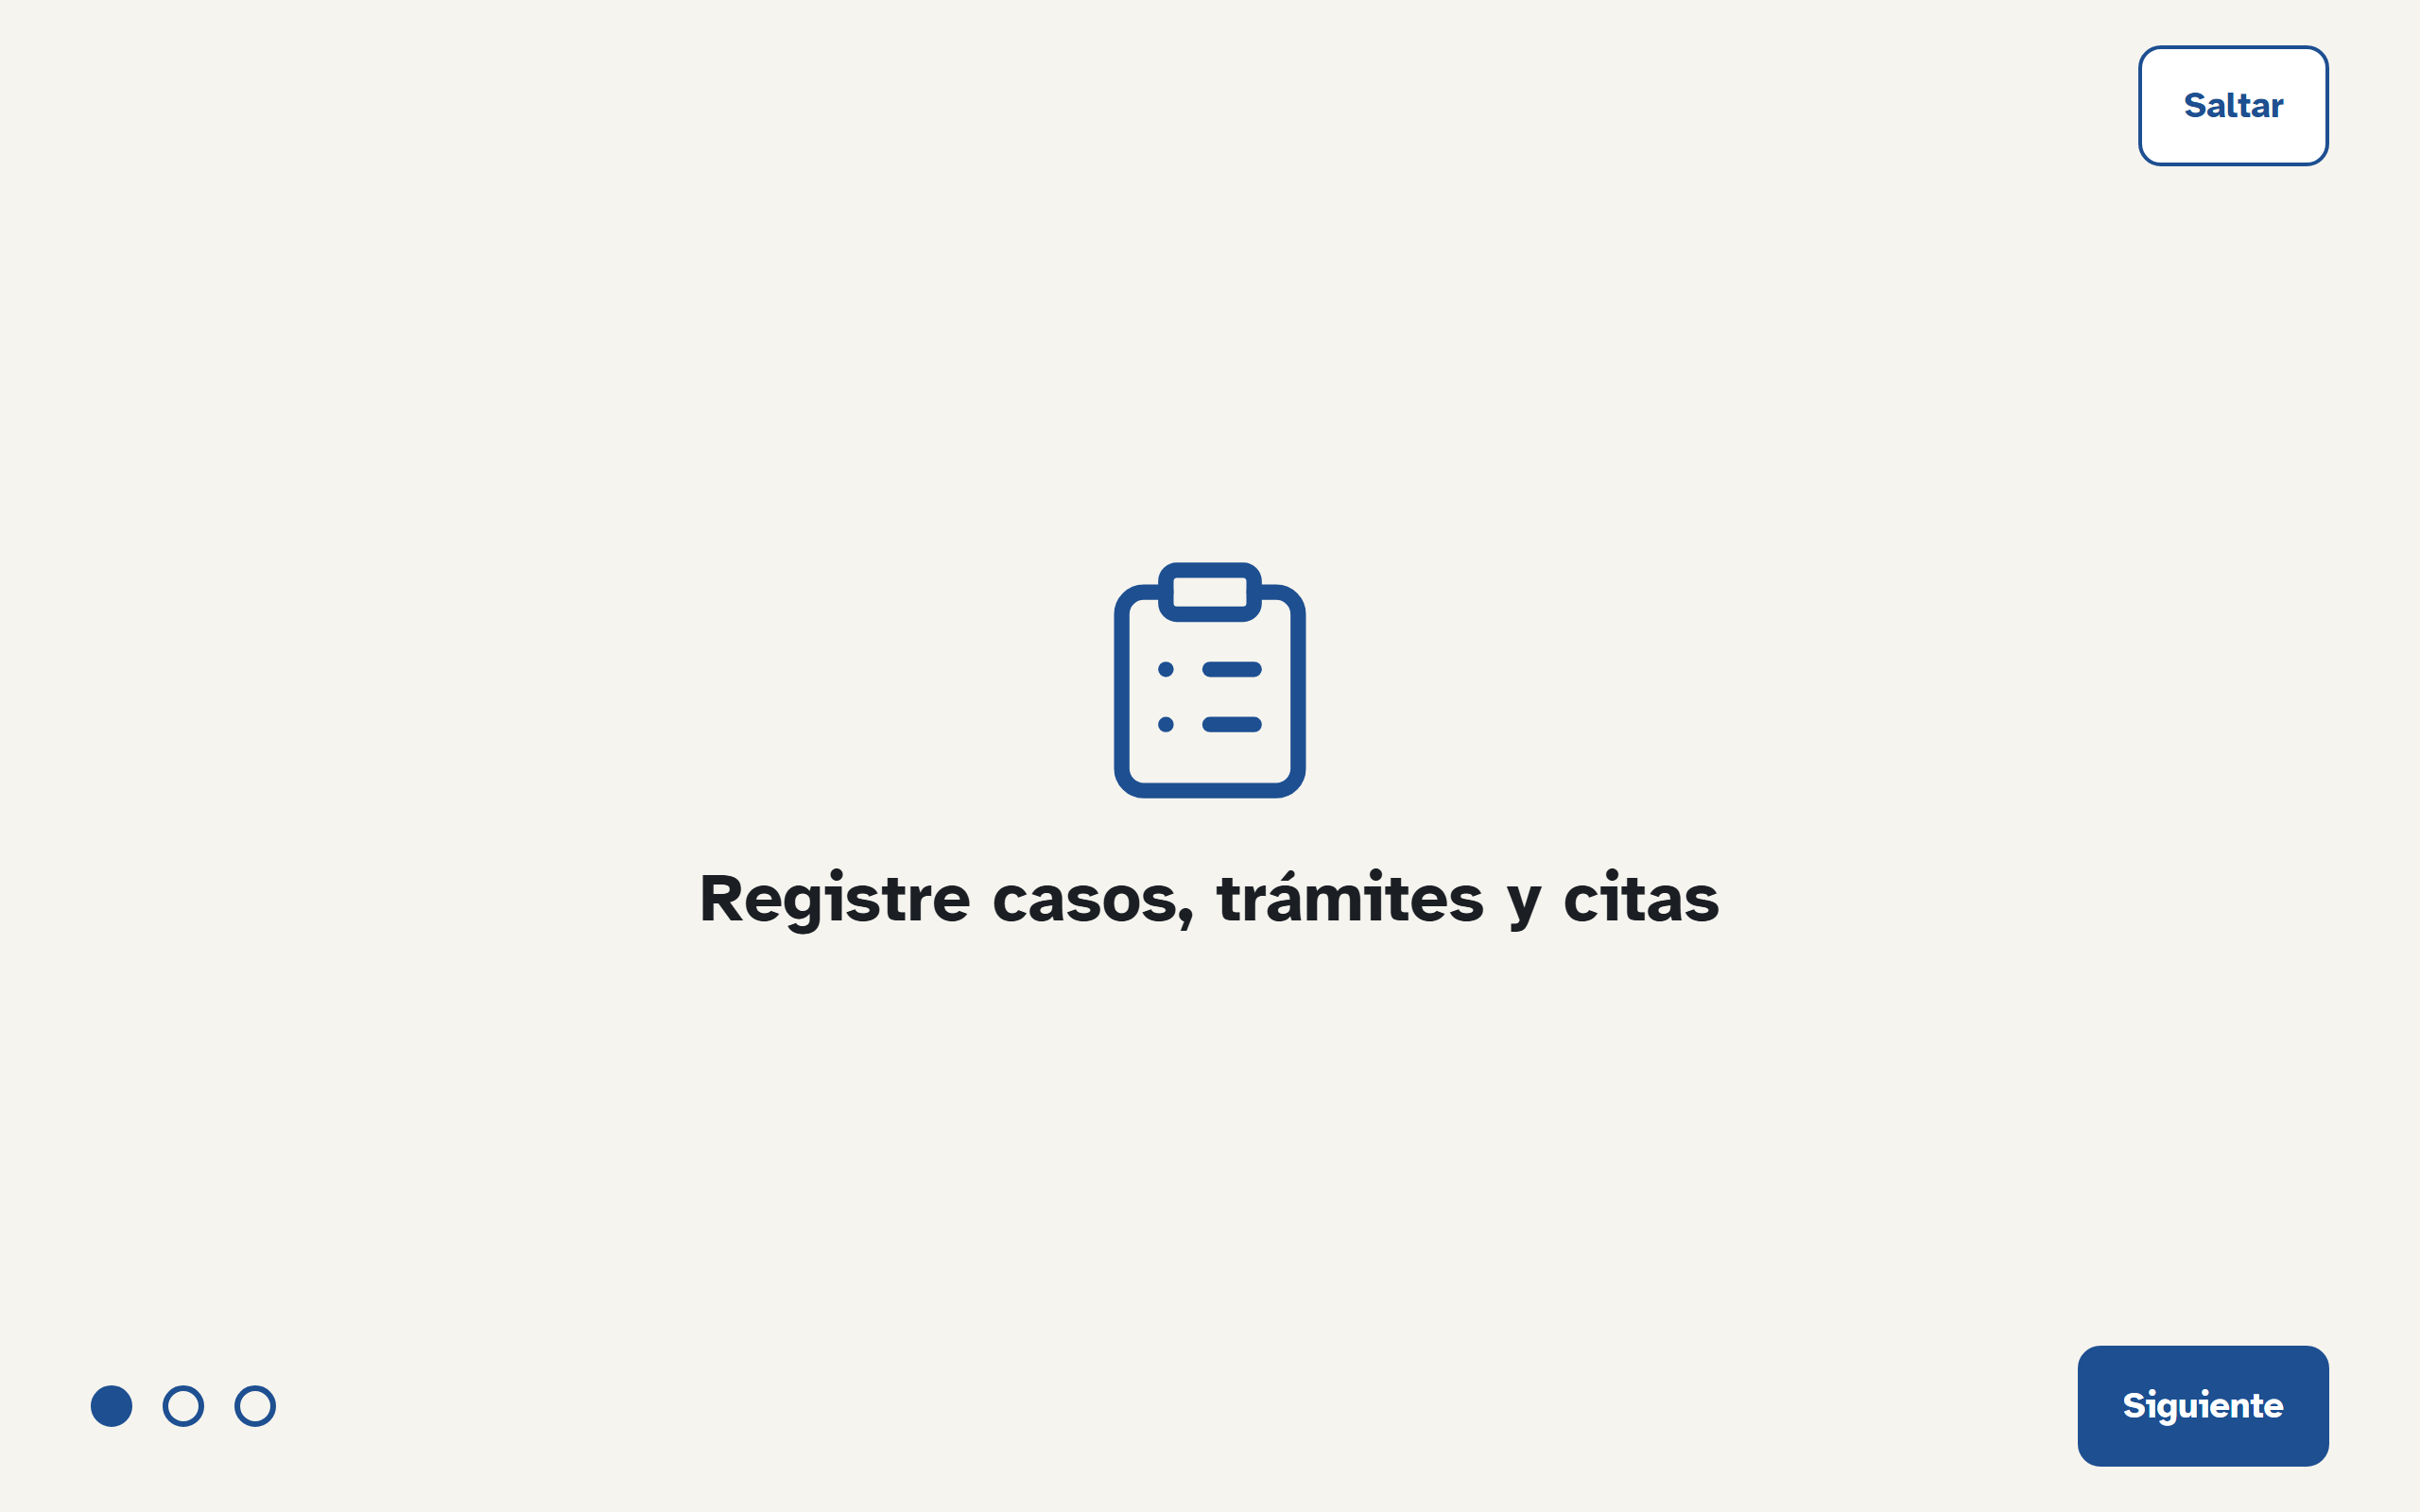
\includegraphics[width=\linewidth]{../../captures/P-00b_introduccion-1.png}\\[-2pt]{\footnotesize\raggedright\textbf{P-00b.} Introducción inicial, pantalla 1 de 3, con [Saltar] visible \emph{(Principios de diseño y heurísticas)}\par}\end{minipage}\hfill
\begin{minipage}[t]{0.49\textwidth}\centering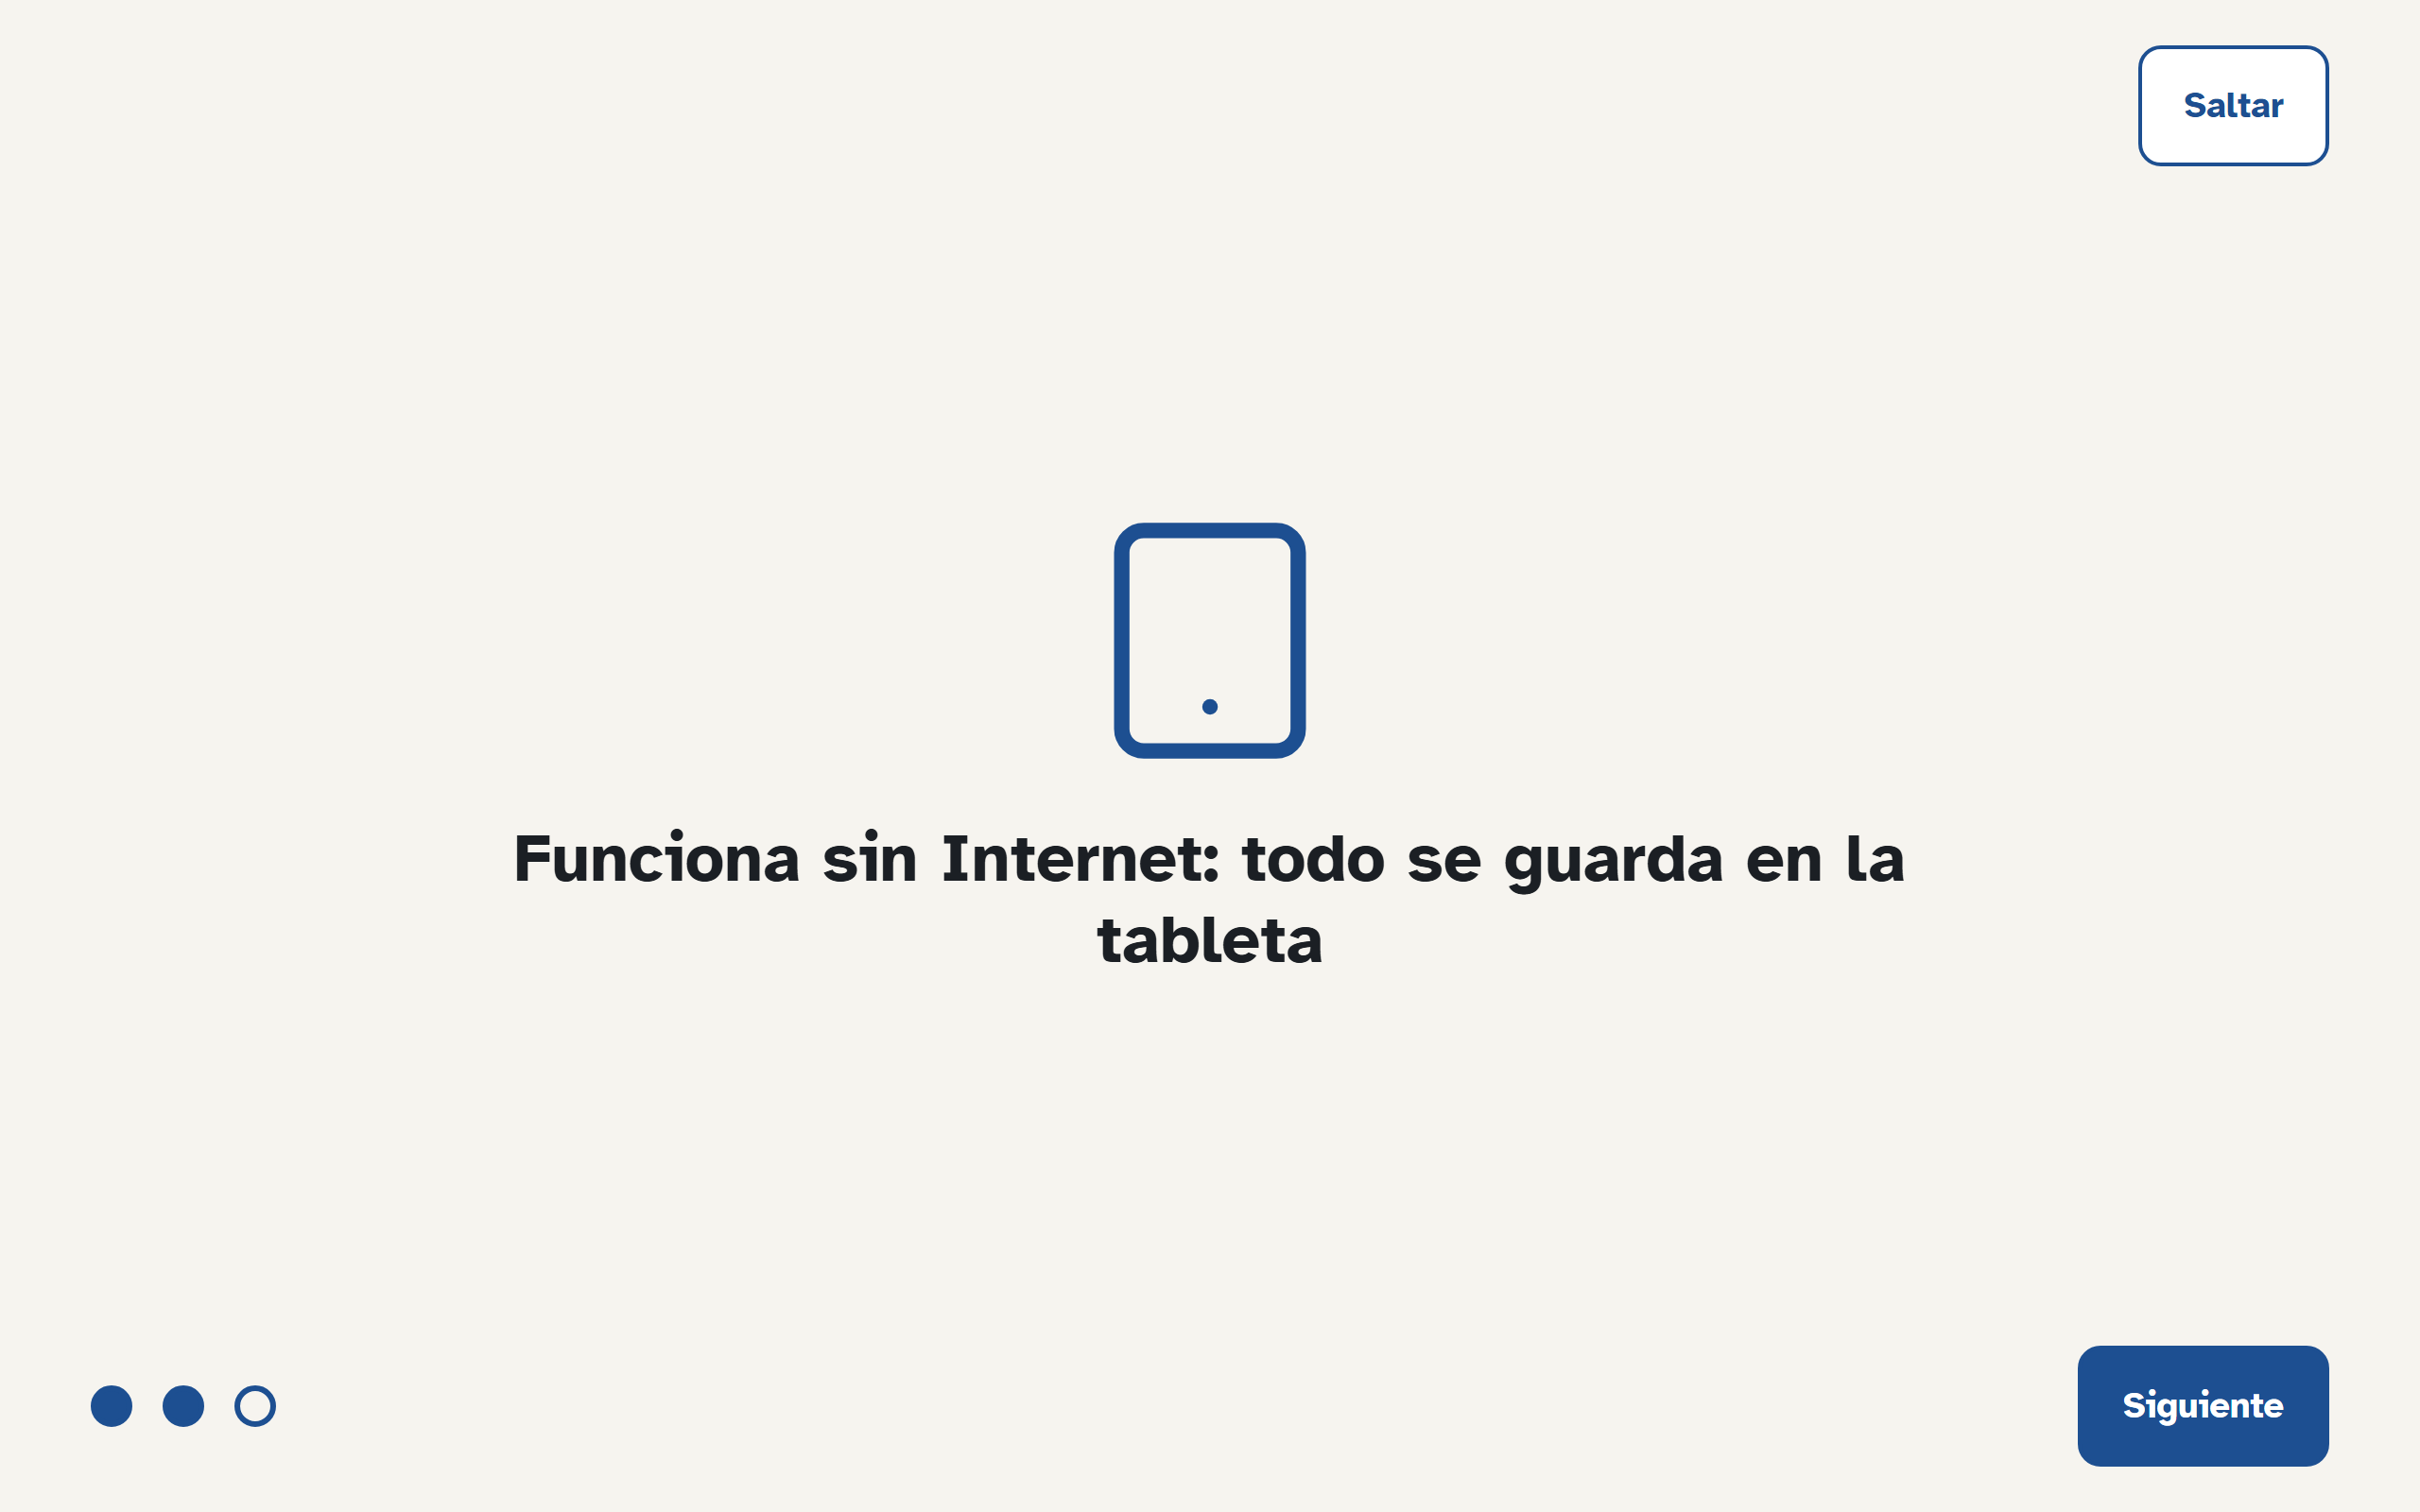
\includegraphics[width=\linewidth]{../../captures/P-00b_introduccion-2.png}\\[-2pt]{\footnotesize\raggedright\textbf{P-00b.} Introducción inicial, pantalla 2 de 3, con [Saltar] visible \emph{(Principios de diseño y heurísticas)}\par}\end{minipage}\par\vspace{8pt}\noindent
\begin{minipage}[t]{0.49\textwidth}\centering
\includegraphics[width=\linewidth]{../../captures/P-00b_introduccion-3.png}\\[-2pt]{\footnotesize\raggedright\textbf{P-00b.} Introducción inicial, pantalla 3 de 3, con [Saltar] visible \emph{(Principios de diseño y heurísticas)}\par}\end{minipage}\hfill
\begin{minipage}[t]{0.49\textwidth}\centering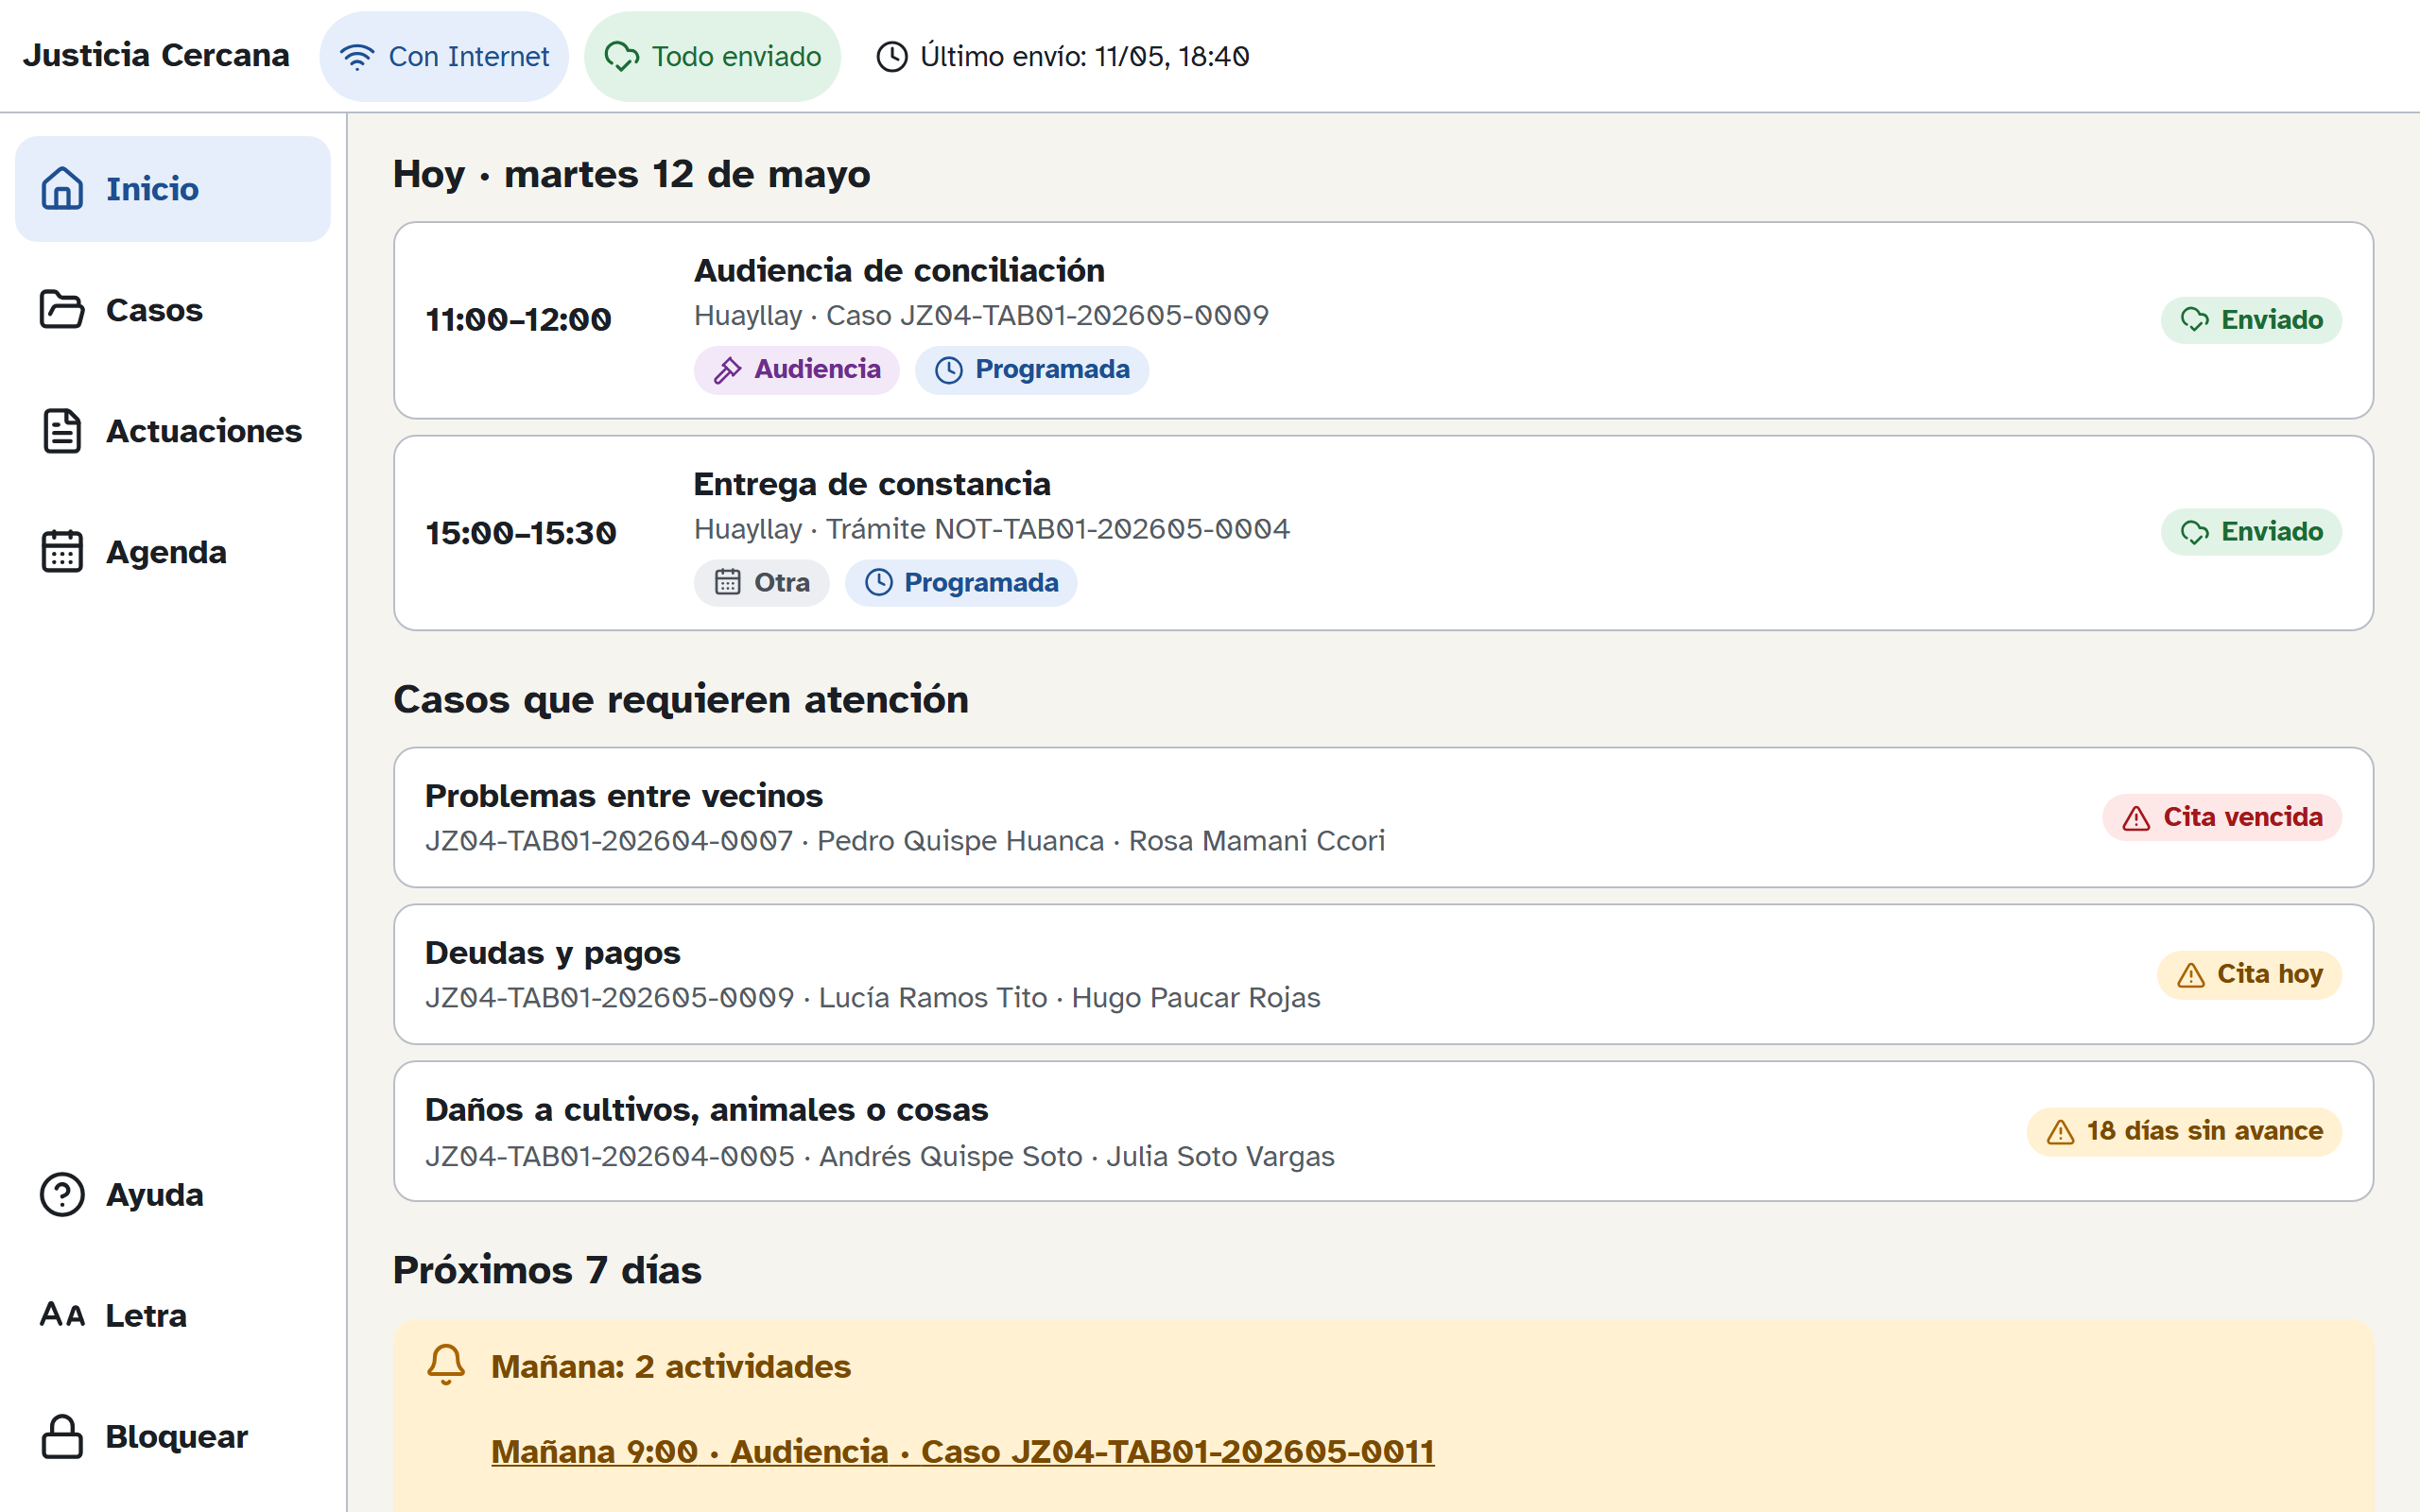
\includegraphics[width=\linewidth]{../../captures/P-01_inicio.png}\\[-2pt]{\footnotesize\raggedright\textbf{P-01.} Inicio: Hoy, casos que requieren atención con motivo en texto, próximos 7 días y accesos grandes \emph{(Cobertura y funcionamiento de los módulos)}\par}\end{minipage}\par\vspace{8pt}\noindent
\begin{minipage}[t]{0.49\textwidth}\centering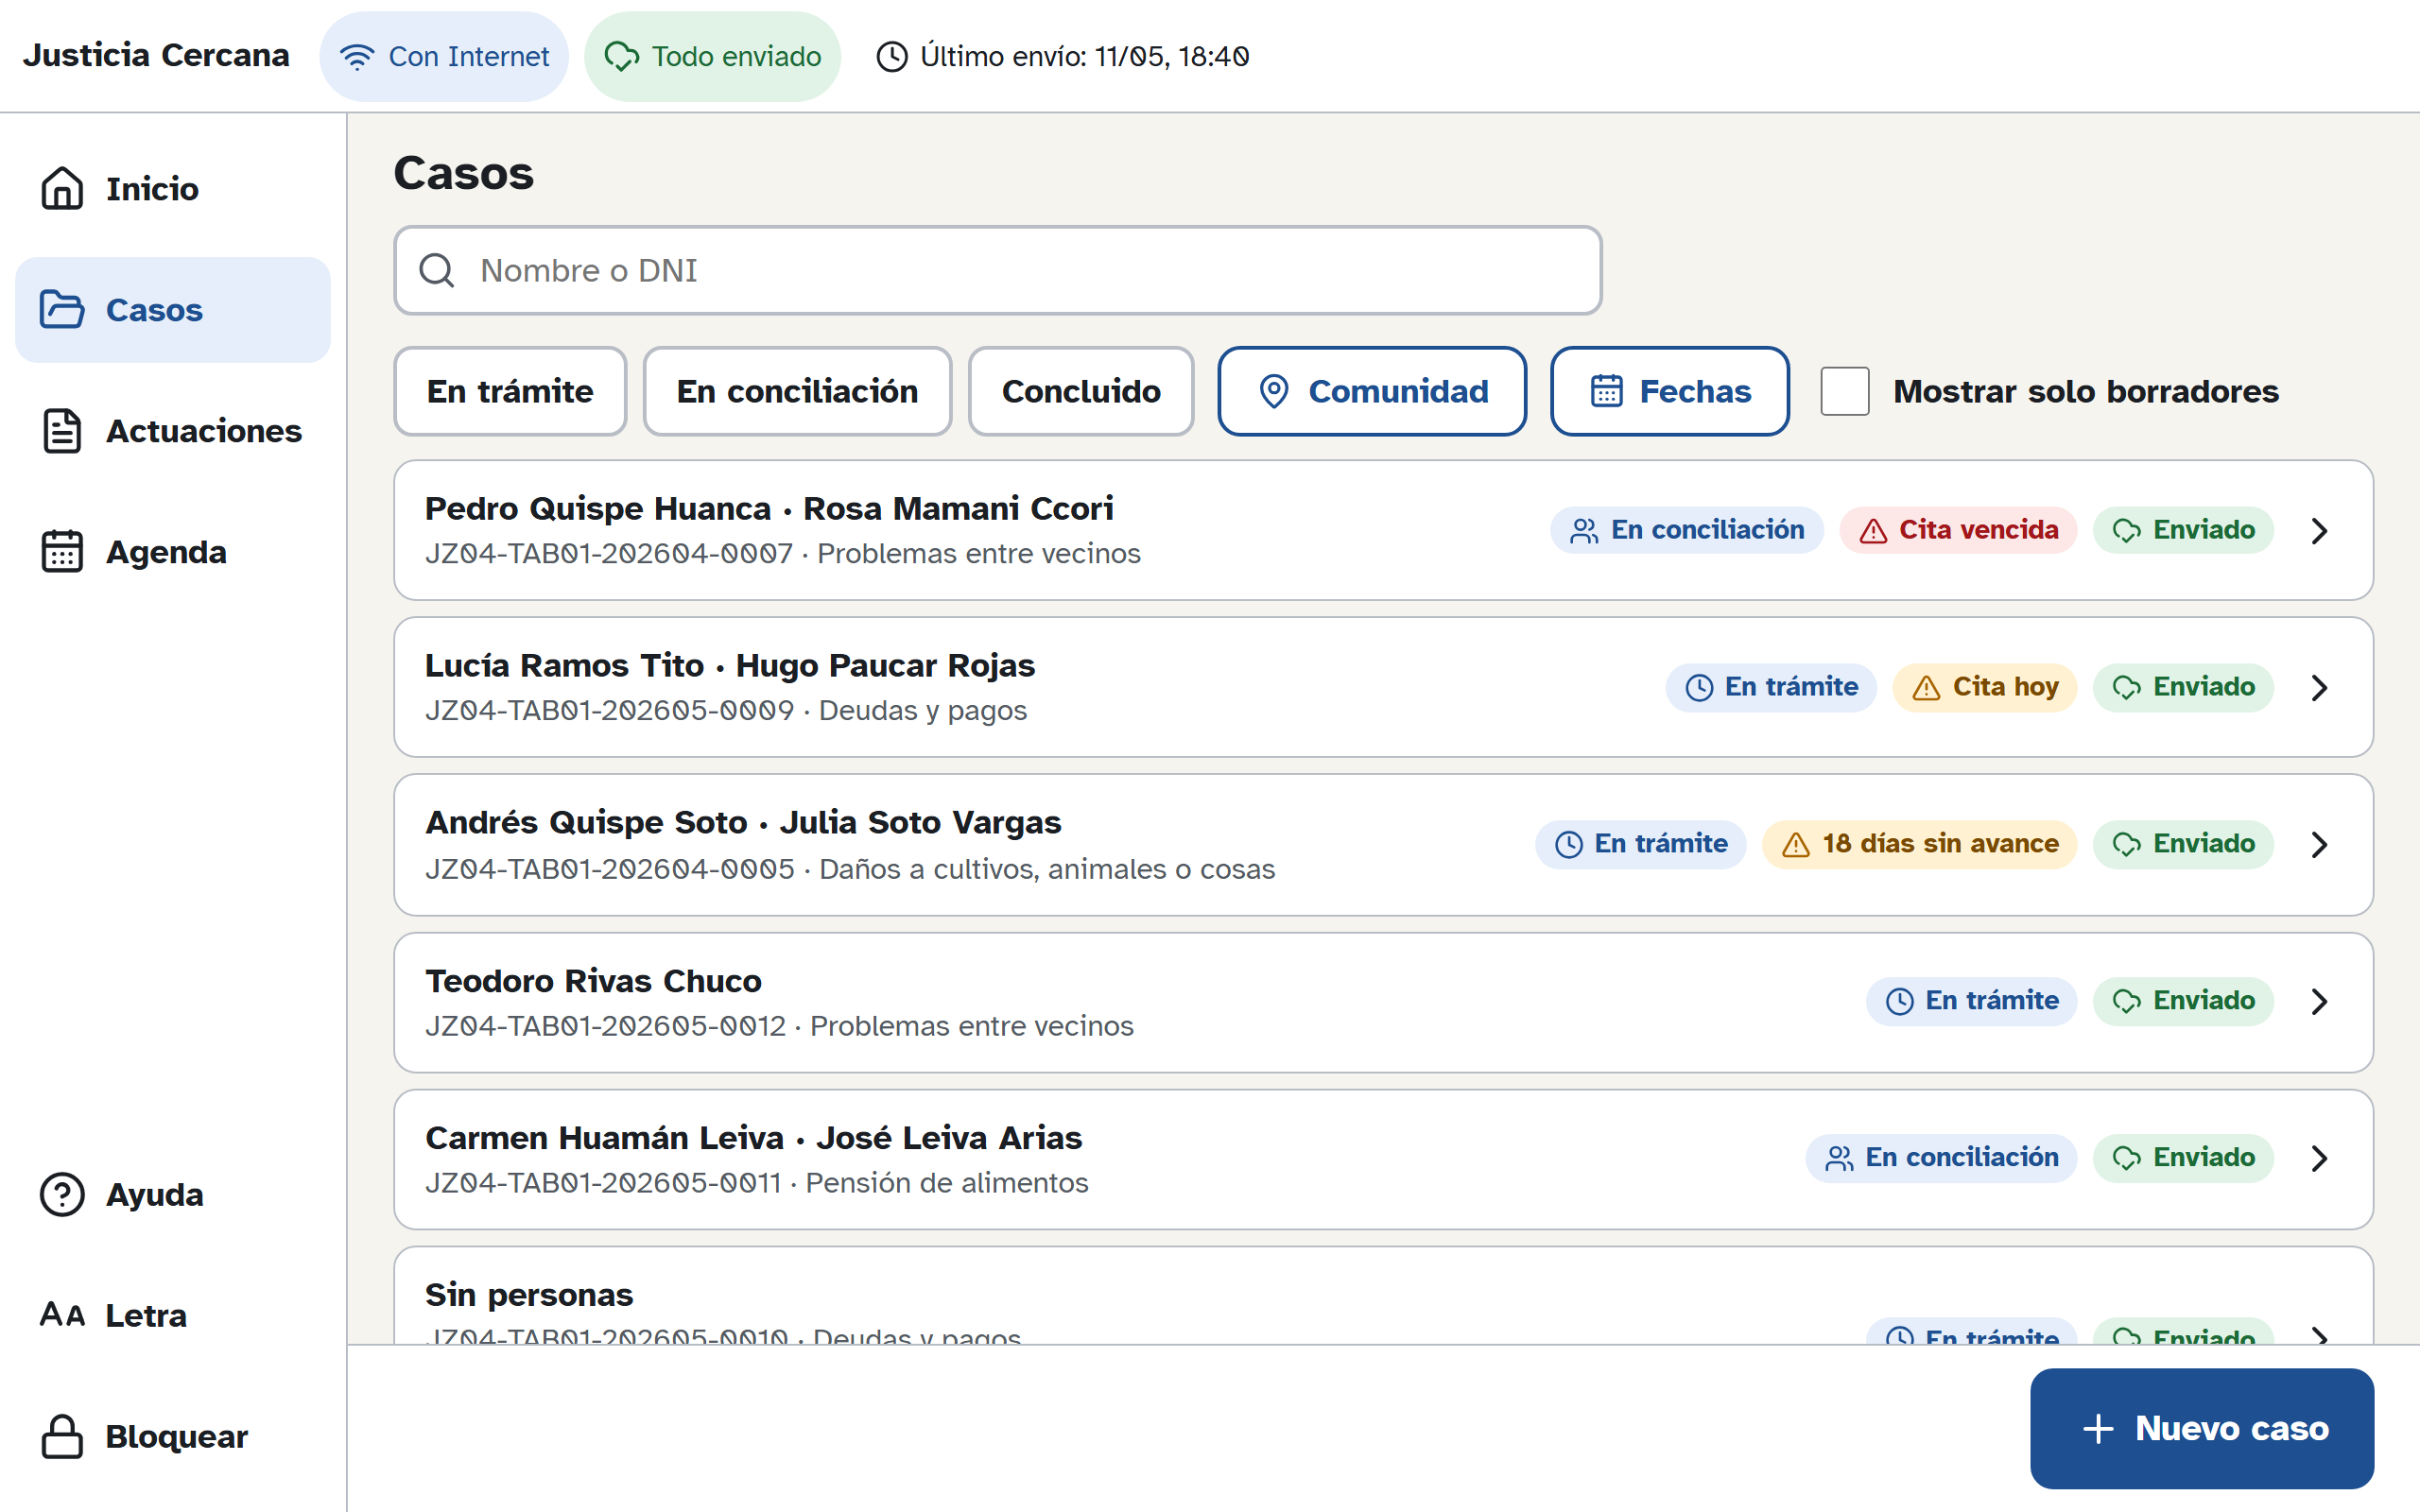
\includegraphics[width=\linewidth]{../../captures/P-02_casos-lista.png}\\[-2pt]{\footnotesize\raggedright\textbf{P-02.} Lista de casos: búsqueda, filtros como botones, motivo de atención, borrador y distintivo por registro \emph{(Cobertura y funcionamiento de los módulos)}\par}\end{minipage}\hfill
\begin{minipage}[t]{0.49\textwidth}\centering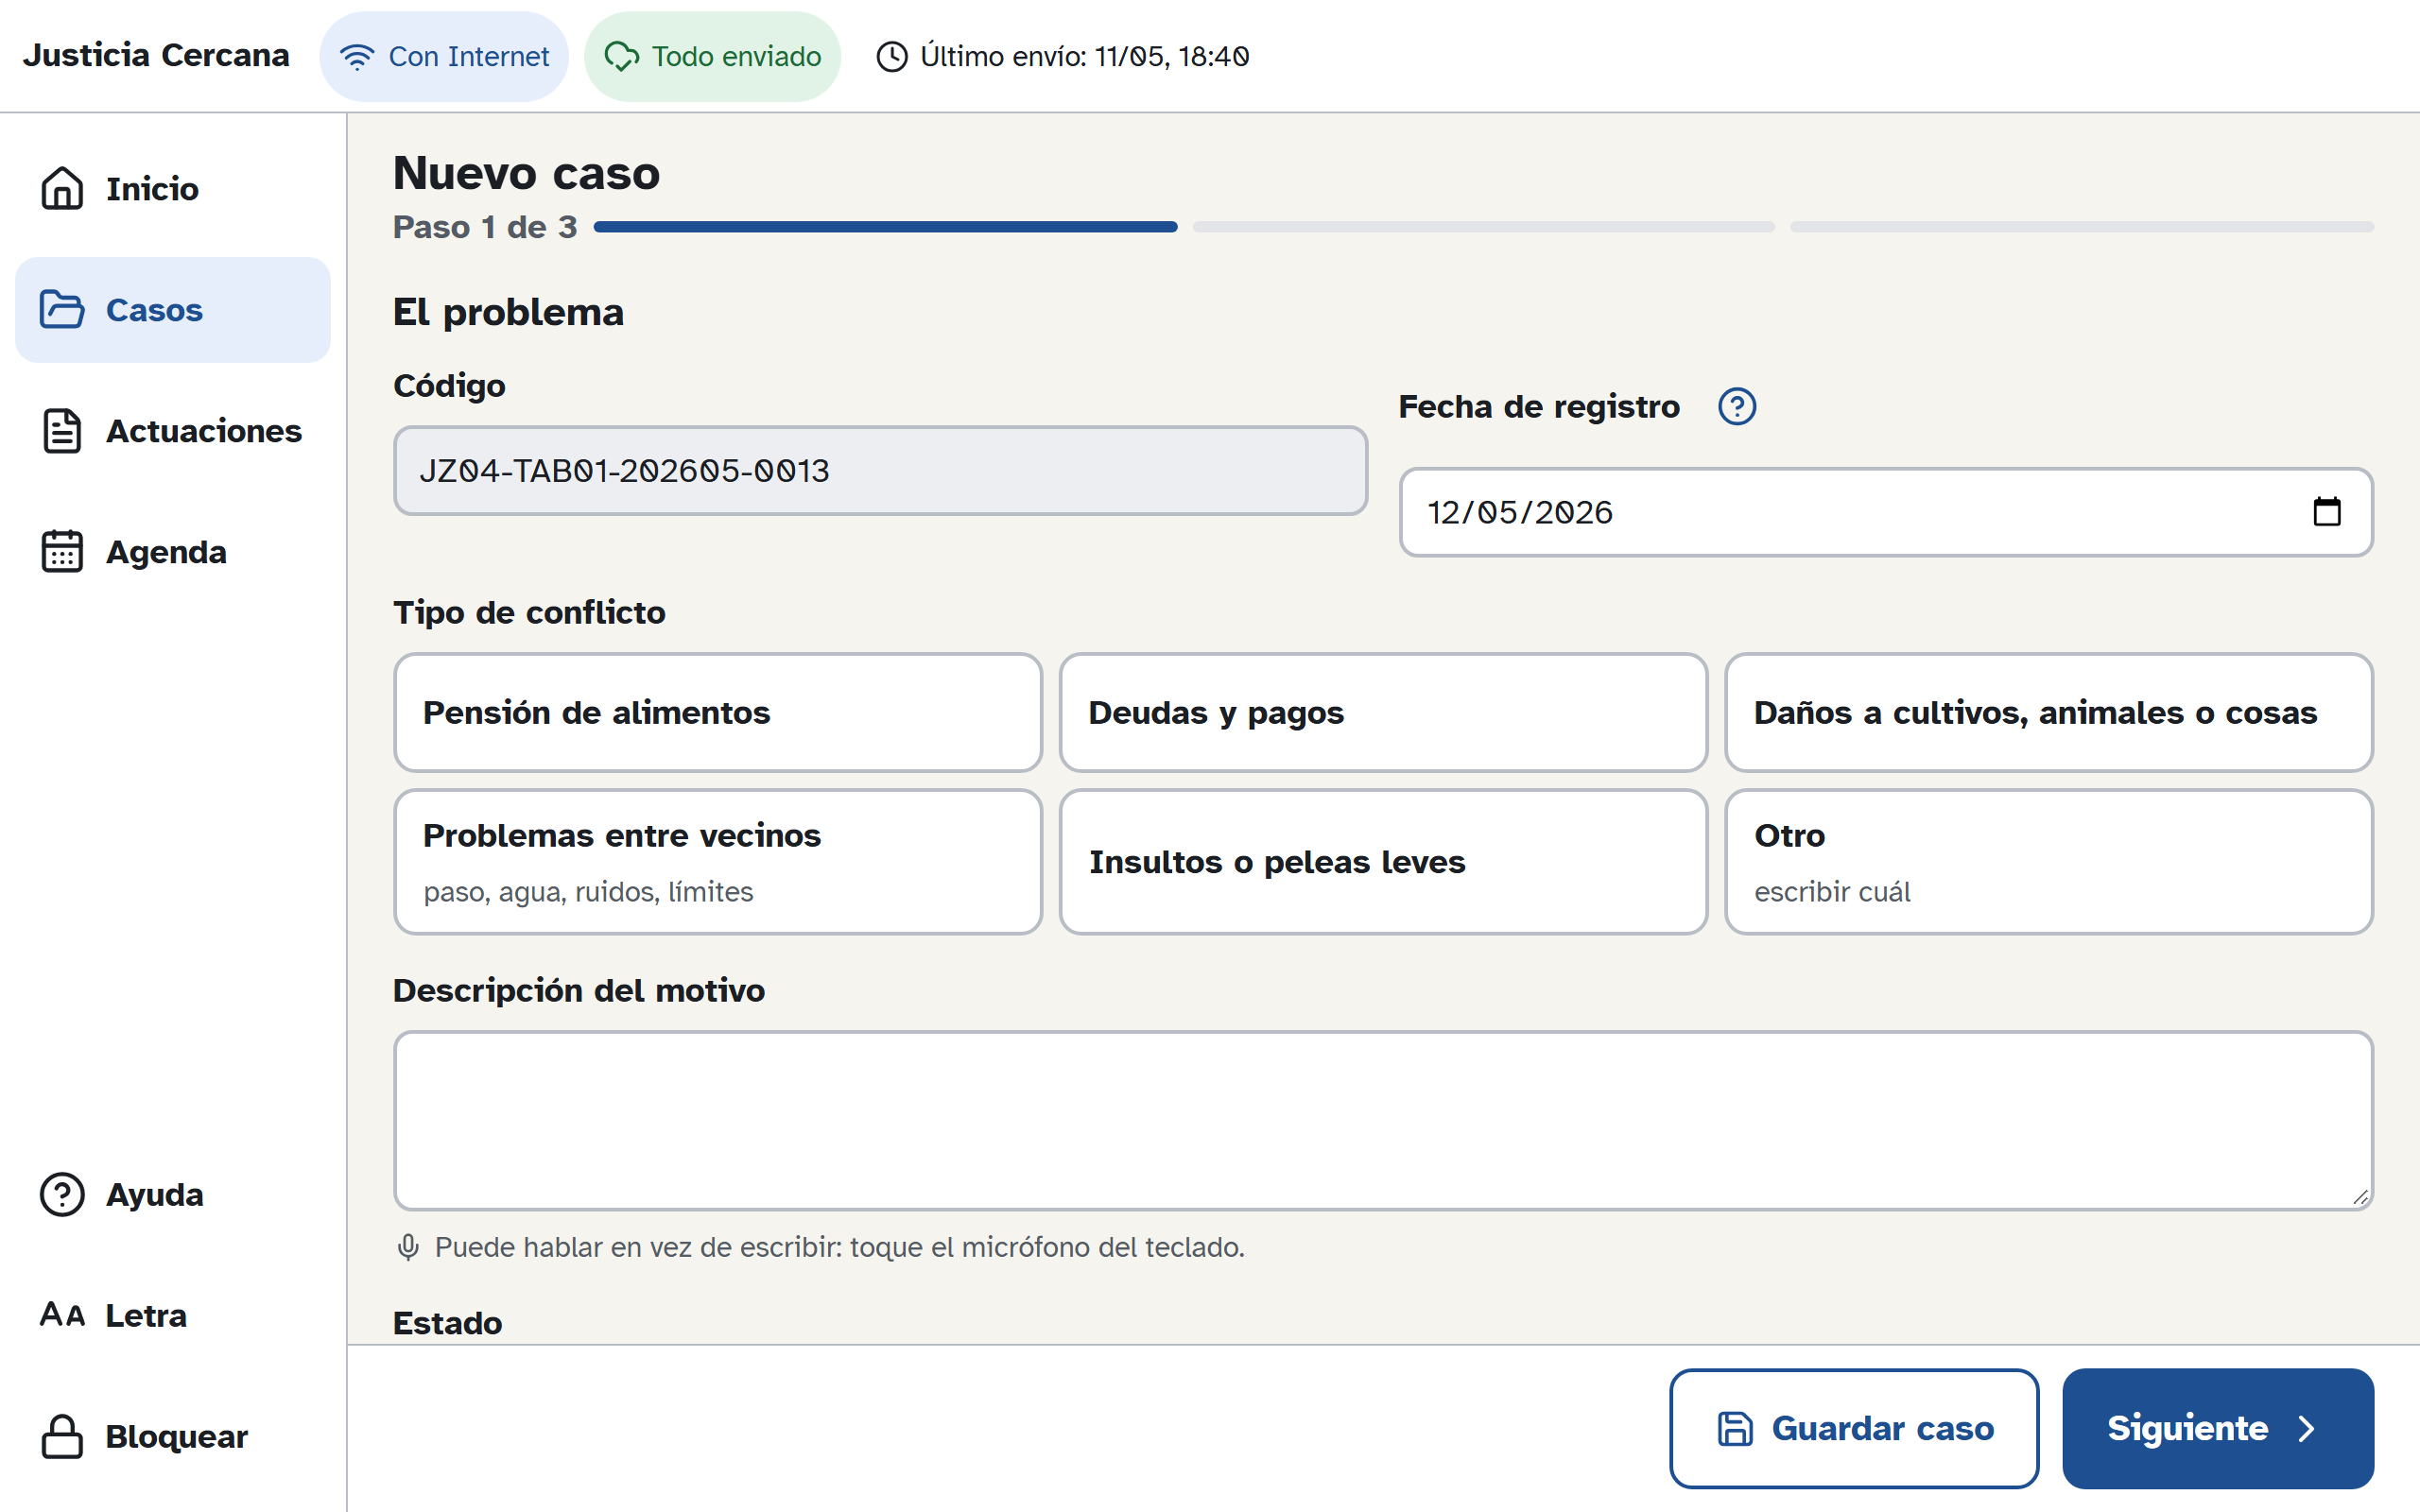
\includegraphics[width=\linewidth]{../../captures/P-03_caso-nuevo.png}\\[-2pt]{\footnotesize\raggedright\textbf{P-03.} Caso nuevo, paso 1 de 3: código generado sin conexión, tipos con botones grandes \emph{(Cobertura y funcionamiento de los módulos)}\par}\end{minipage}\par\vspace{8pt}\noindent
\begin{minipage}[t]{0.49\textwidth}\centering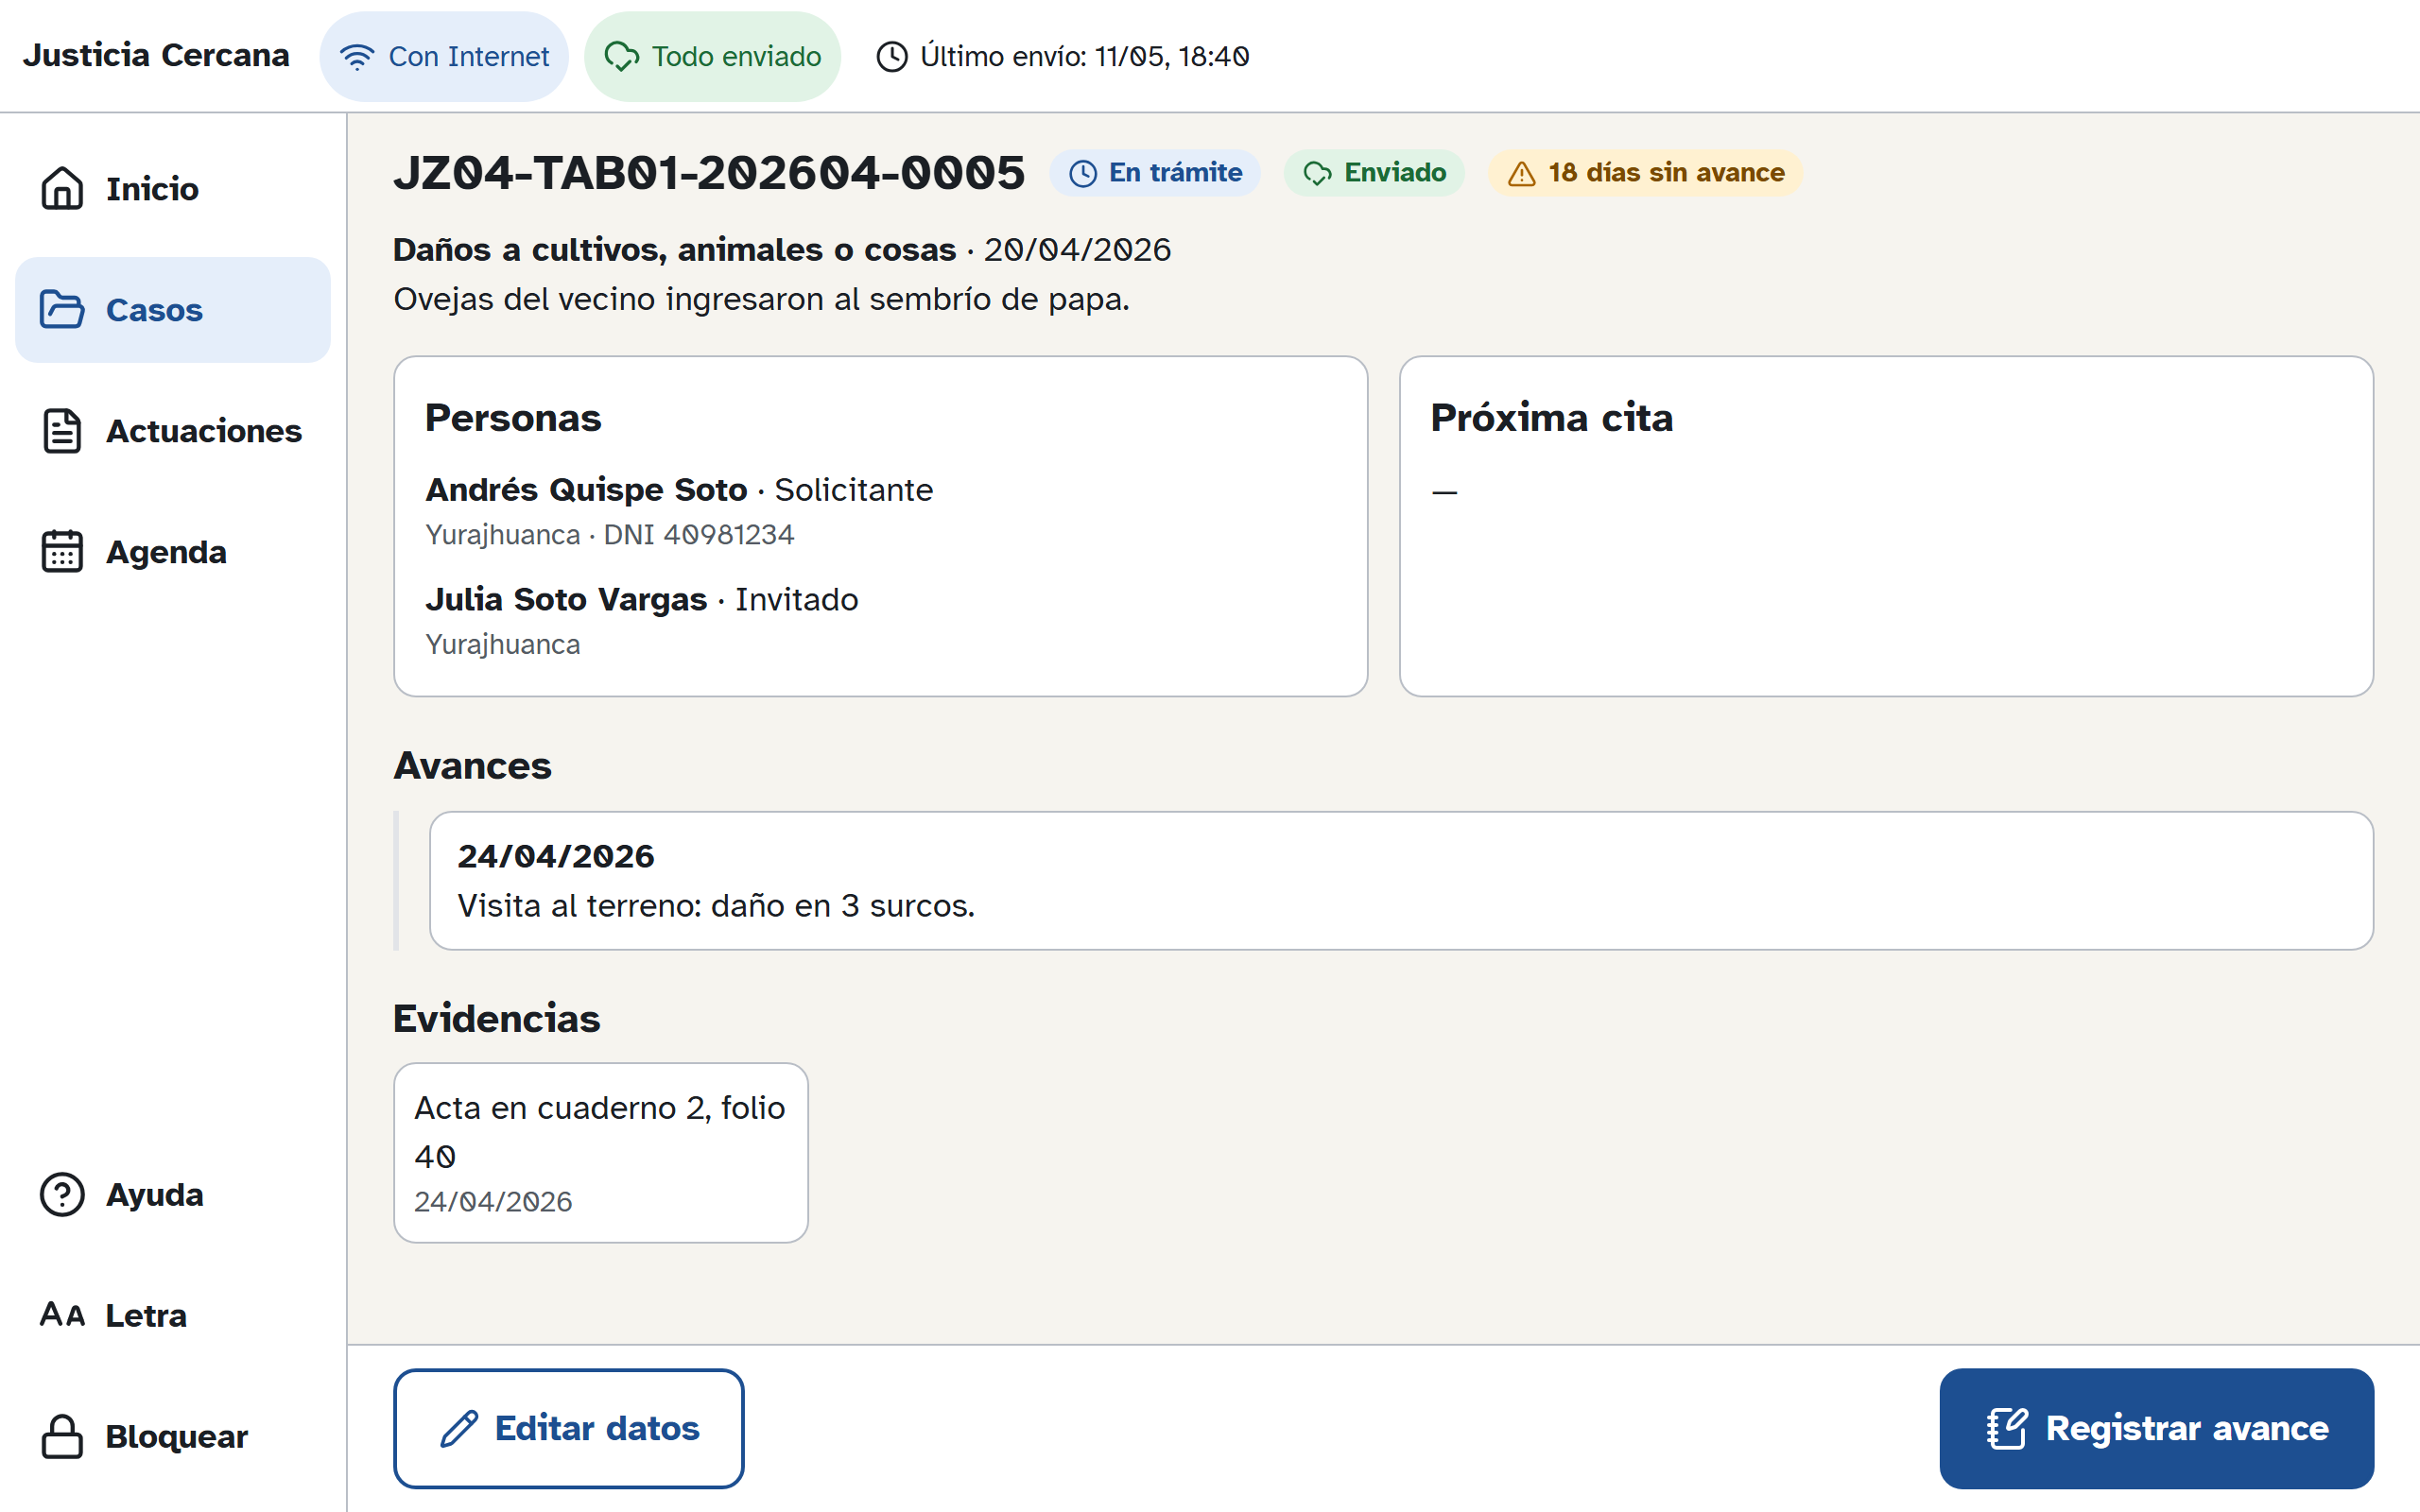
\includegraphics[width=\linewidth]{../../captures/P-04_caso-detalle.png}\\[-2pt]{\footnotesize\raggedright\textbf{P-04.} Detalle: estado, distintivo, motivo ``15+ días sin avance'', historial, evidencias; [Registrar avance] abajo a la derecha \emph{(Cobertura y funcionamiento de los módulos)}\par}\end{minipage}\hfill
\begin{minipage}[t]{0.49\textwidth}\centering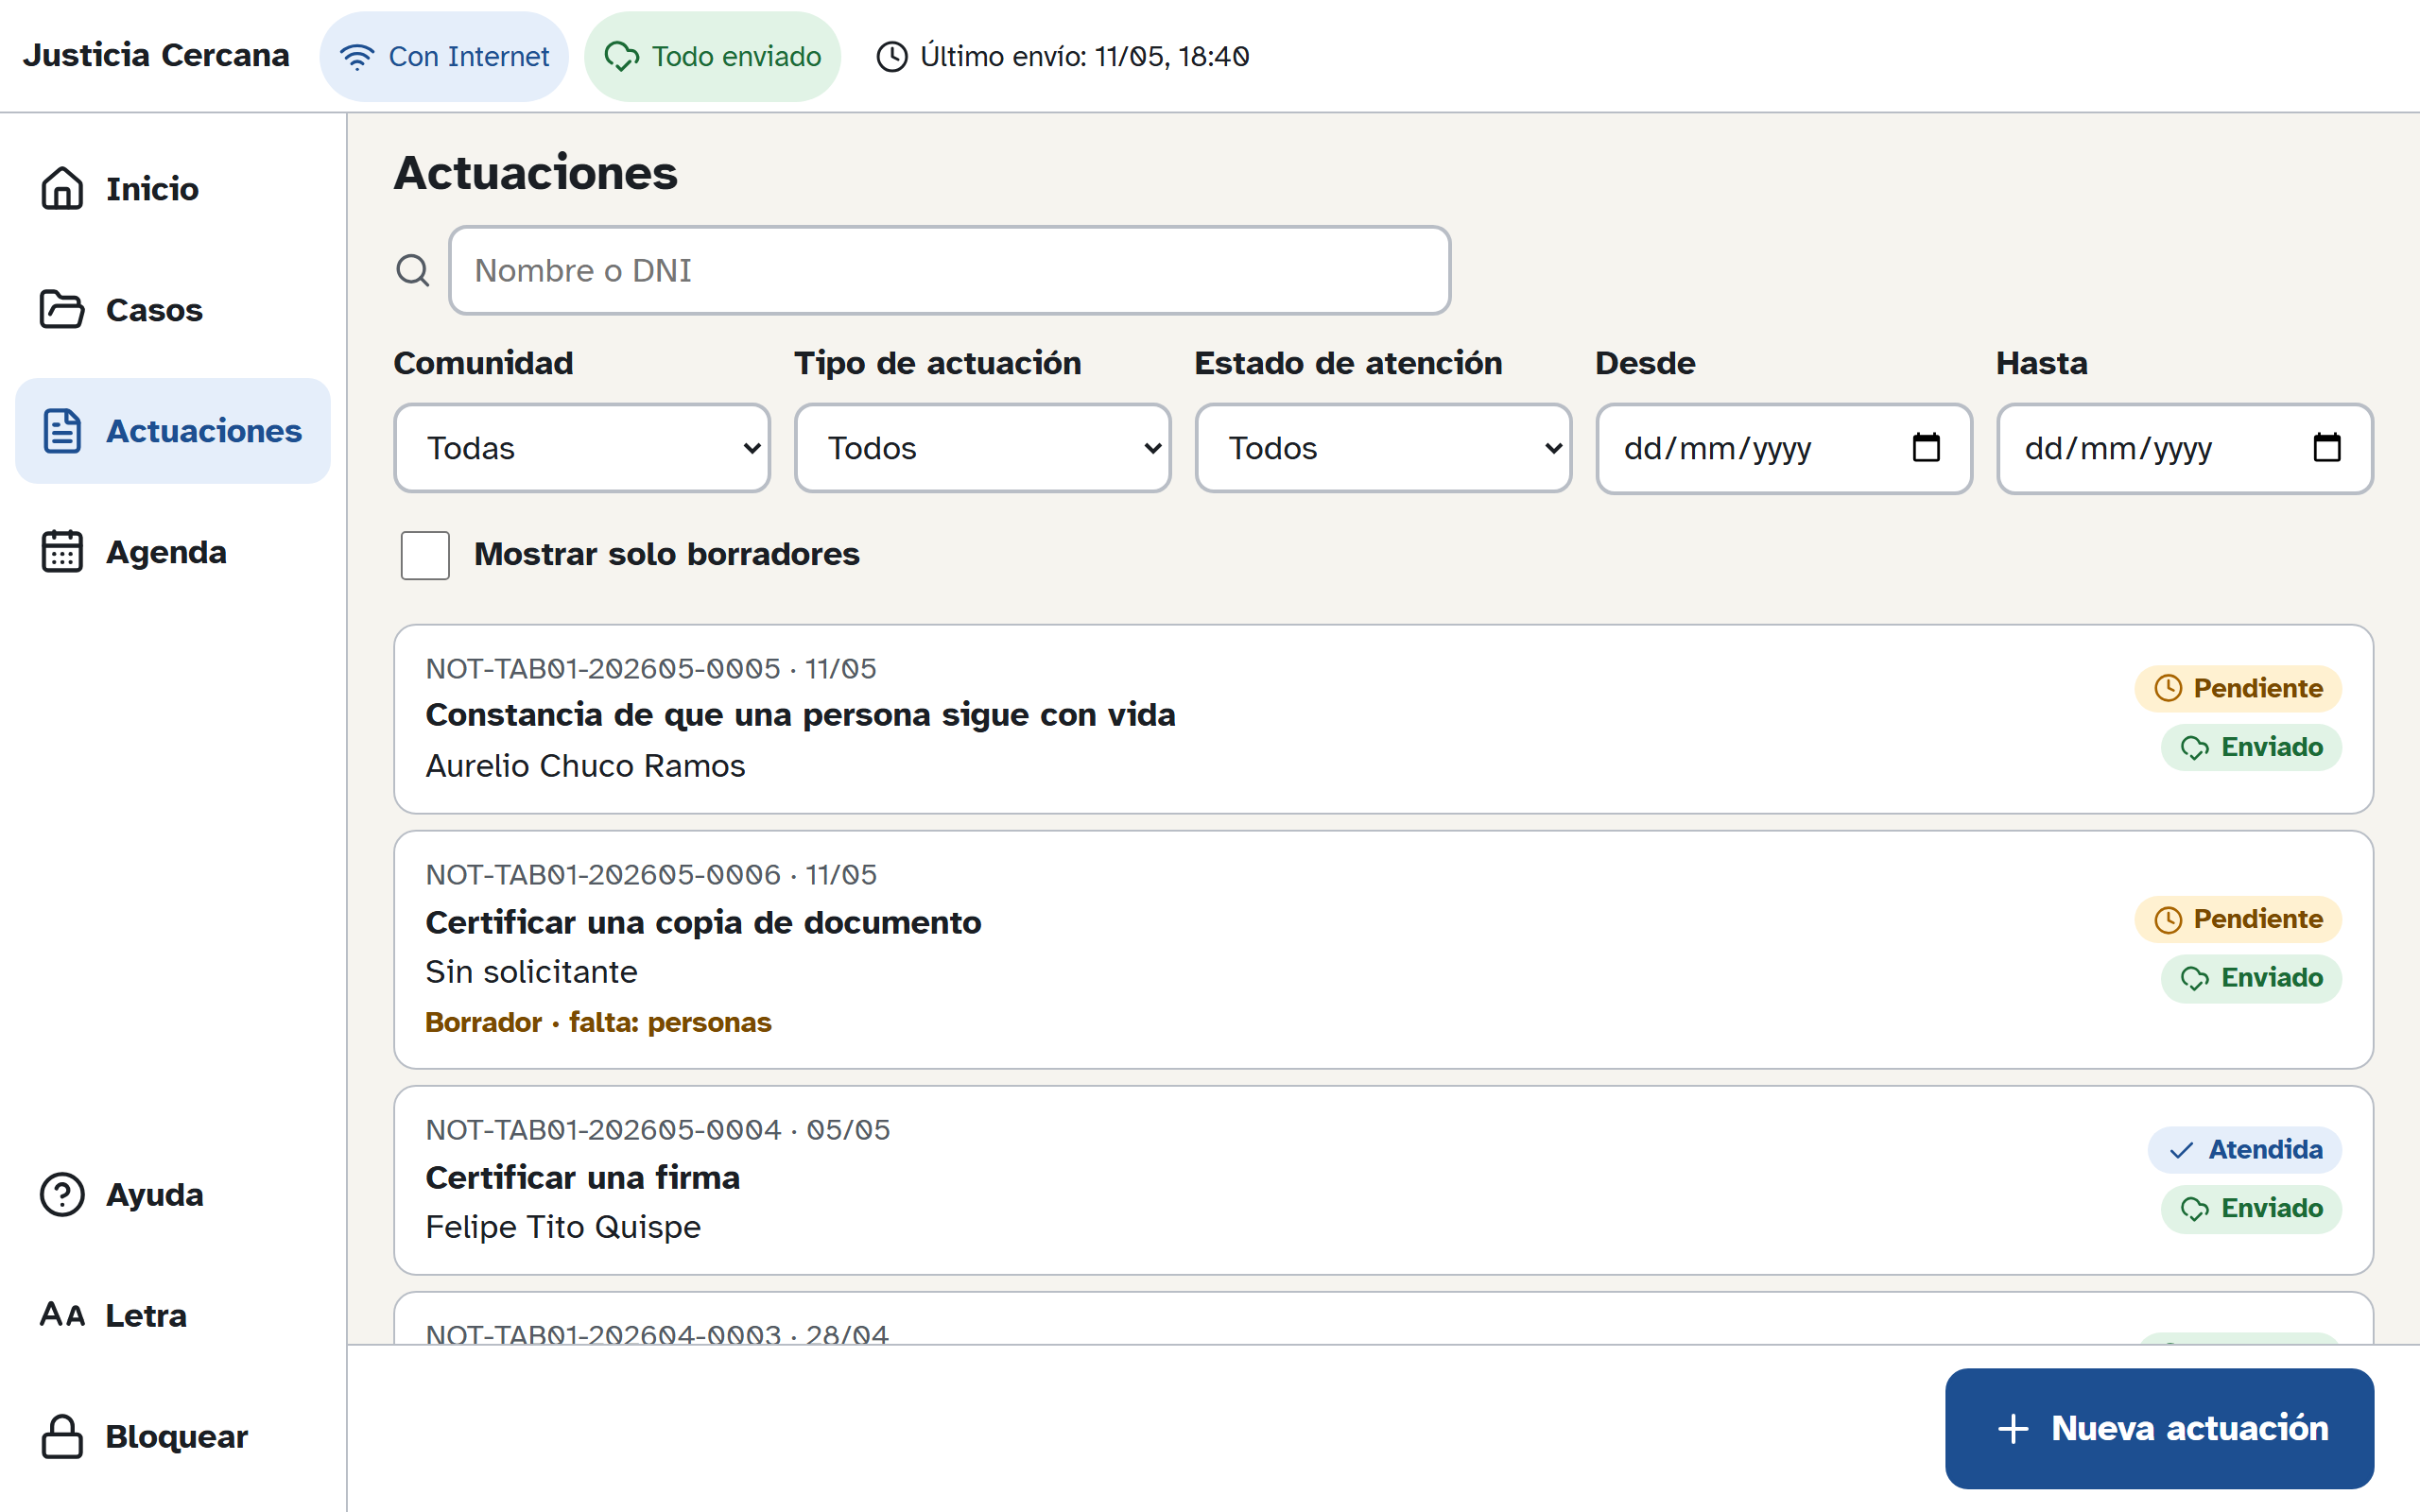
\includegraphics[width=\linewidth]{../../captures/P-05_actuaciones-lista.png}\\[-2pt]{\footnotesize\raggedright\textbf{P-05.} Lista de actuaciones con estado de atención, borrador y distintivo \emph{(Cobertura y funcionamiento de los módulos)}\par}\end{minipage}\par\vspace{8pt}\noindent
\begin{minipage}[t]{0.49\textwidth}\centering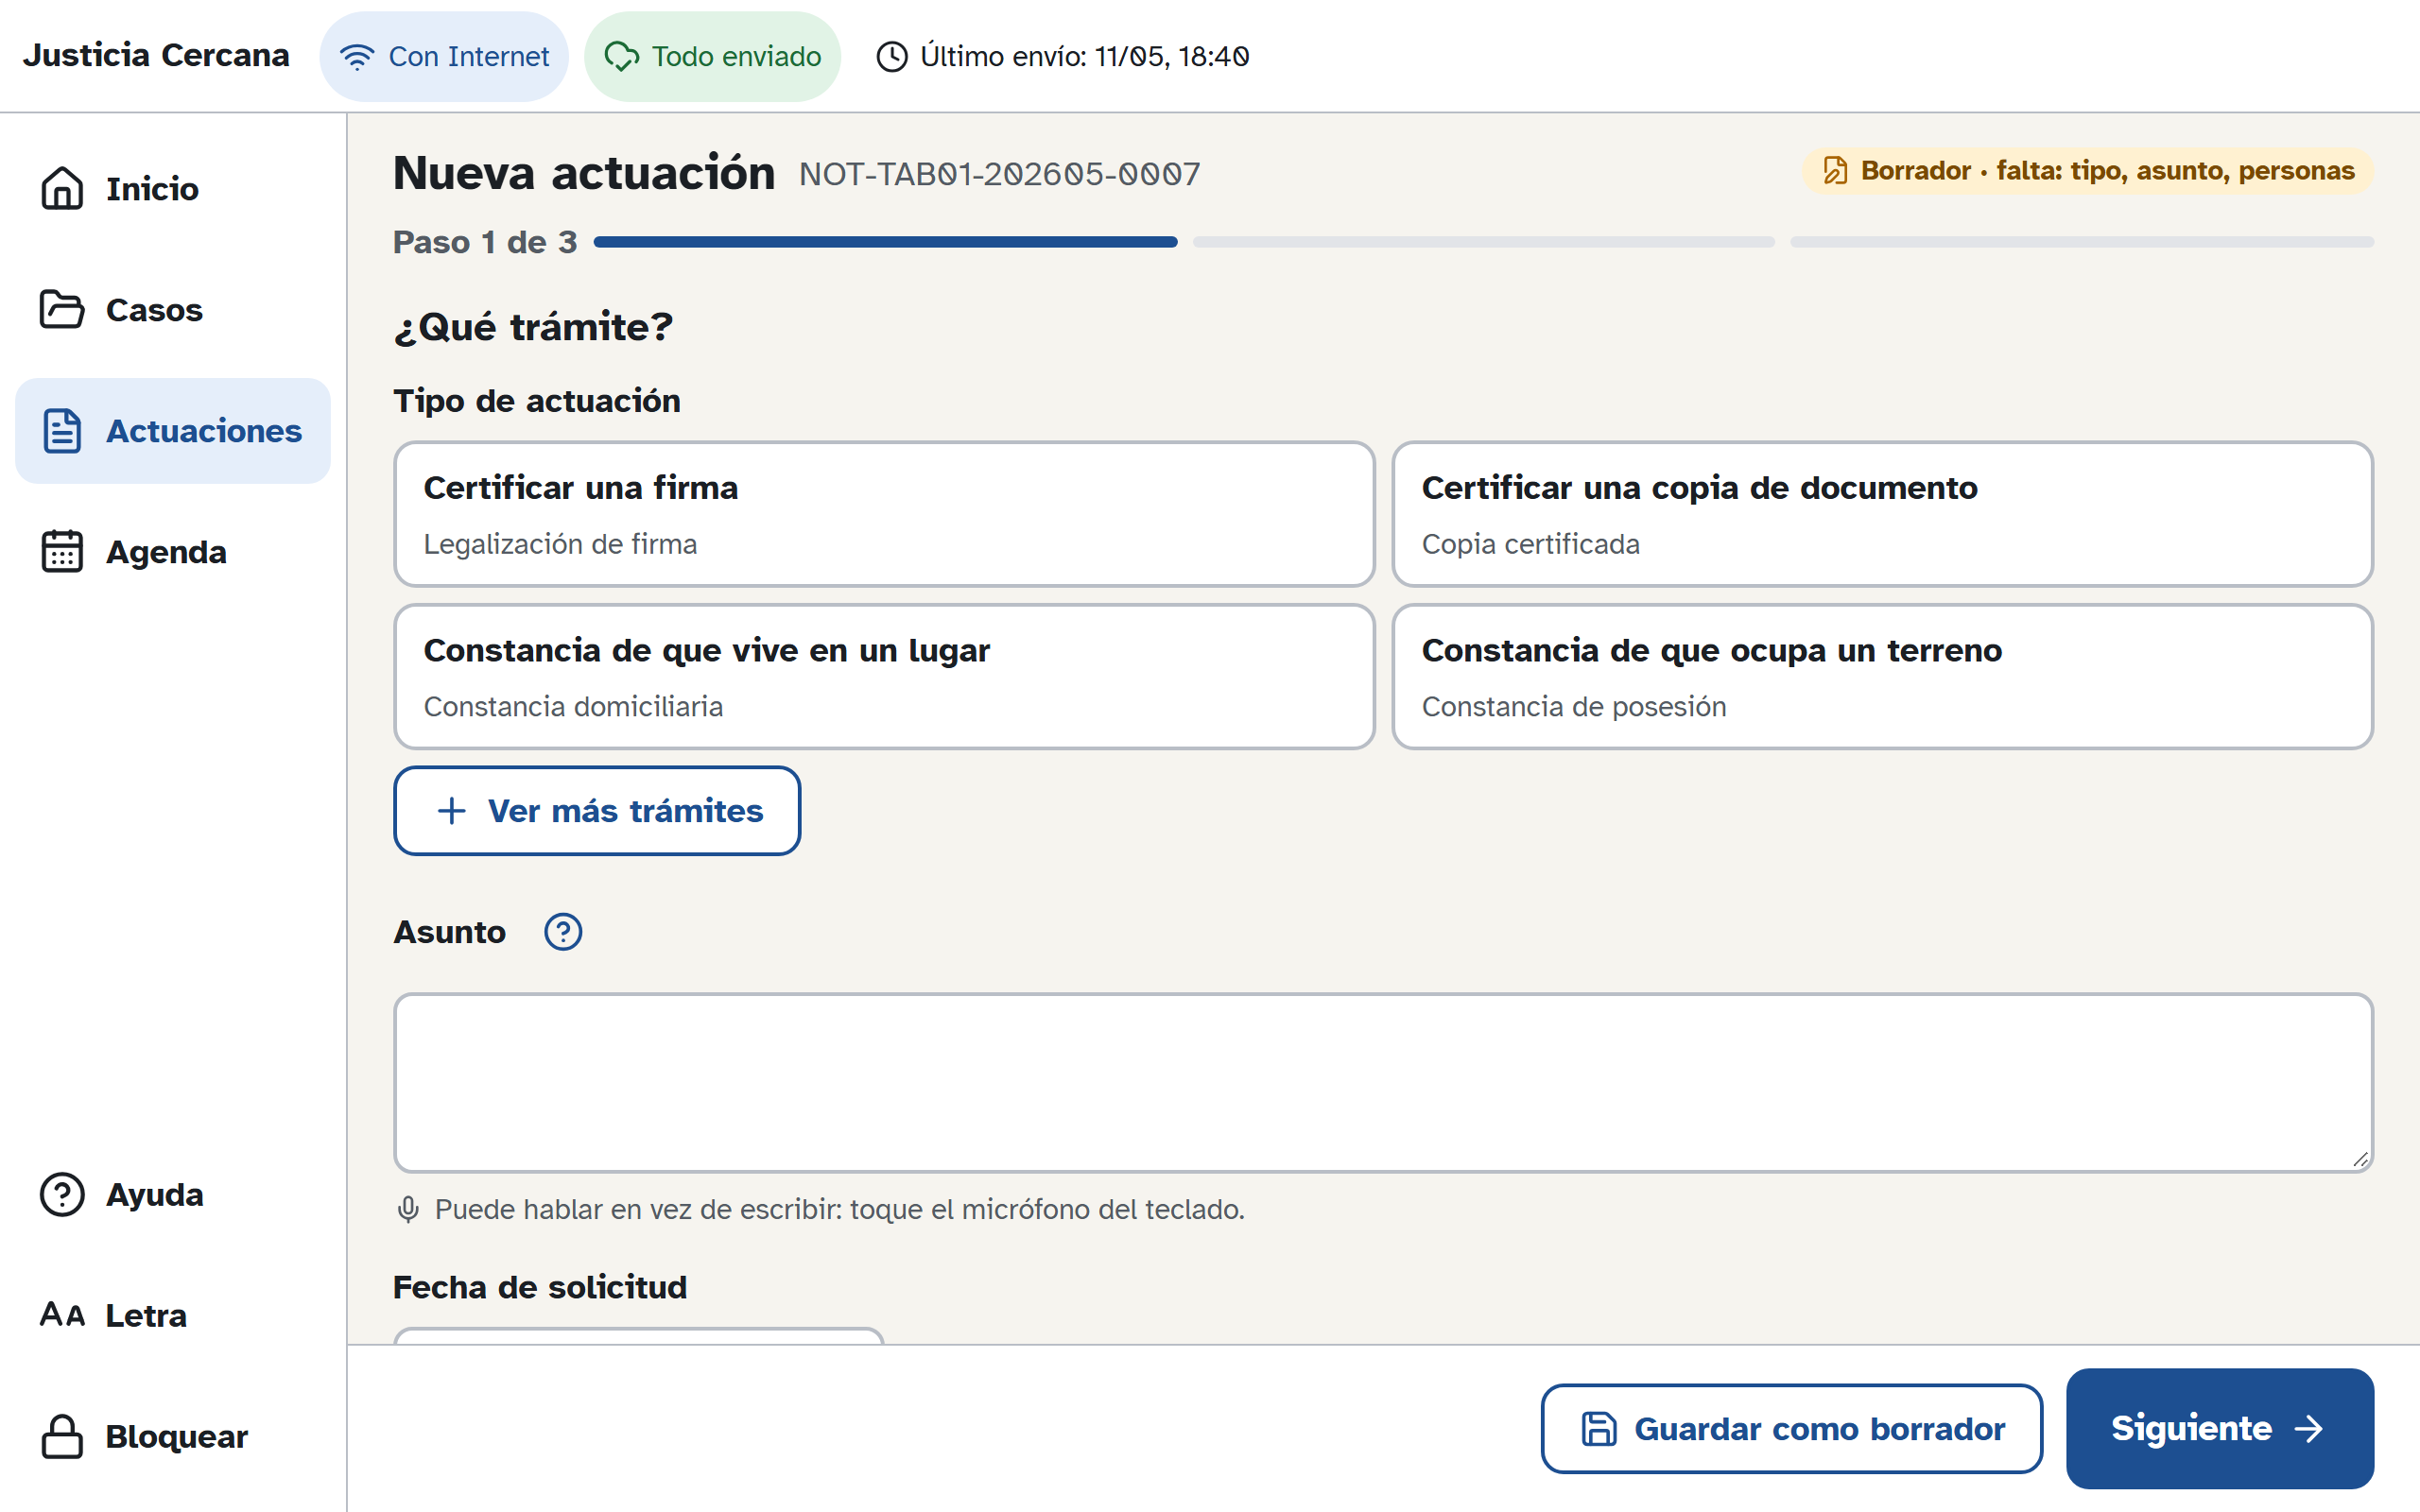
\includegraphics[width=\linewidth]{../../captures/P-06_actuacion-nueva.png}\\[-2pt]{\footnotesize\raggedright\textbf{P-06.} Actuación nueva, paso 1: 4 tarjetas en lenguaje cotidiano + [Ver más trámites] \emph{(Cobertura y funcionamiento de los módulos)}\par}\end{minipage}\hfill
\begin{minipage}[t]{0.49\textwidth}\centering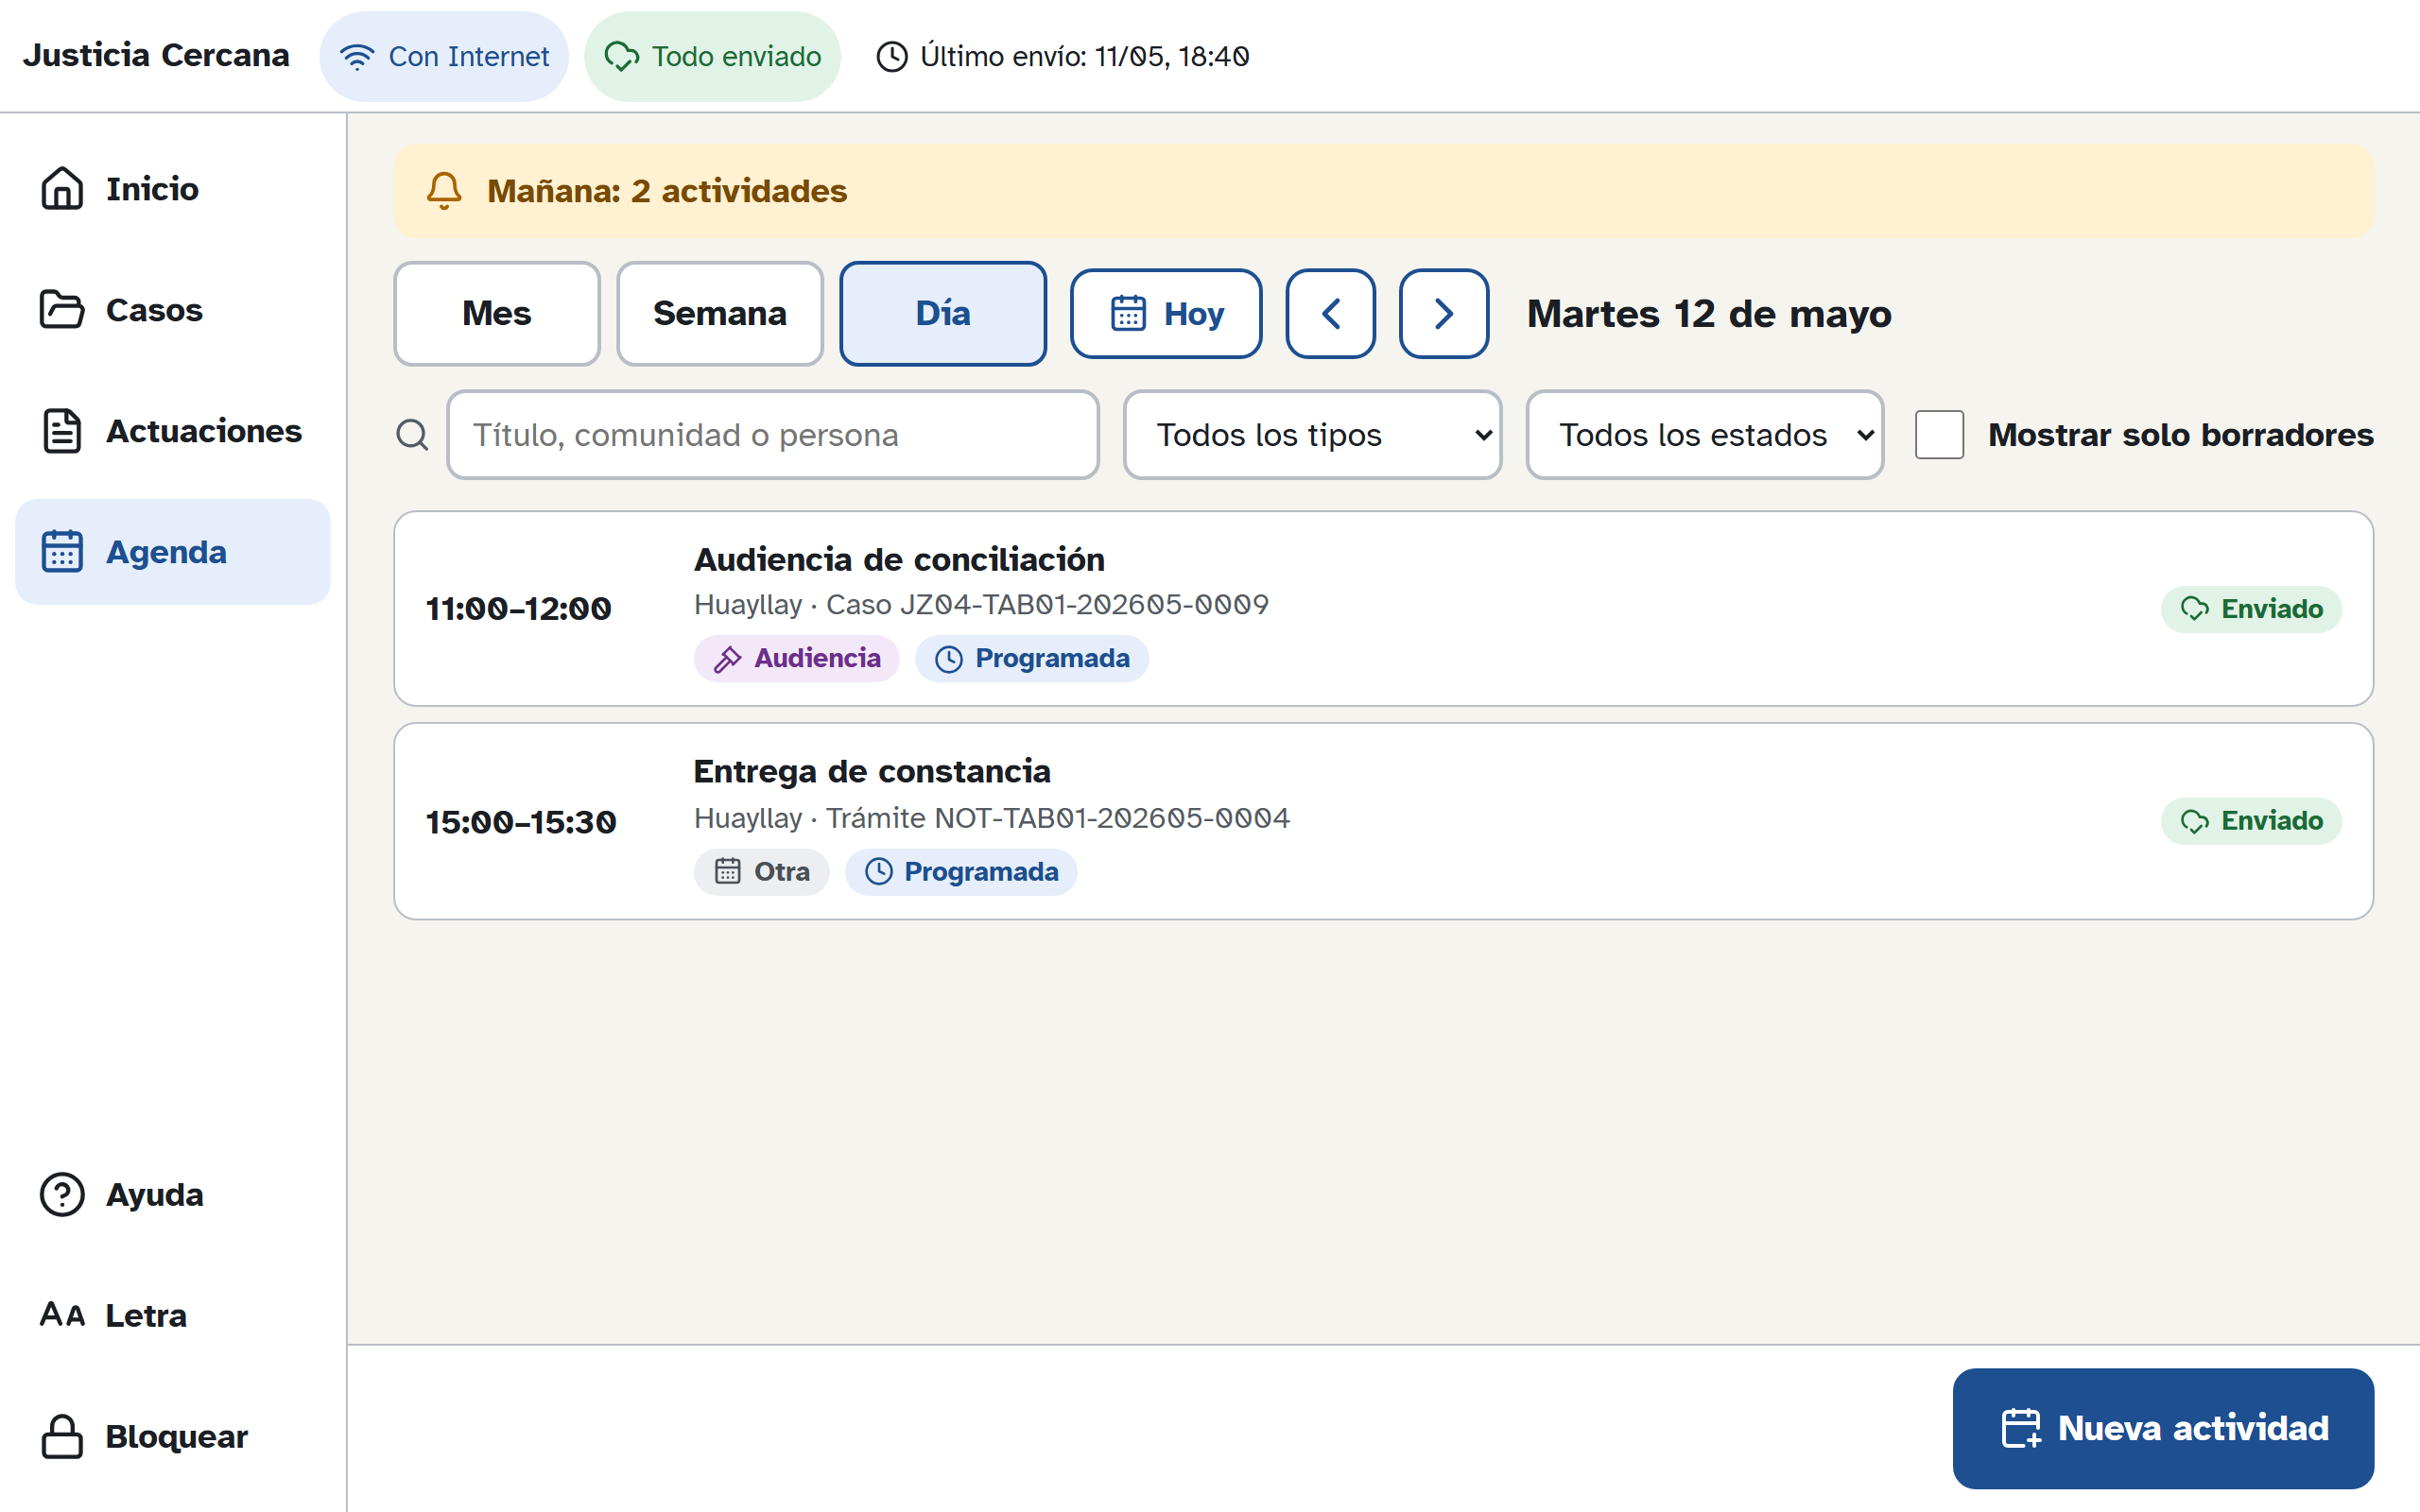
\includegraphics[width=\linewidth]{../../captures/P-07_agenda-dia.png}\\[-2pt]{\footnotesize\raggedright\textbf{P-07.} Agenda Día (hoy) \emph{(Cobertura y funcionamiento de los módulos)}\par}\end{minipage}\par\vspace{8pt}\noindent
\begin{minipage}[t]{0.49\textwidth}\centering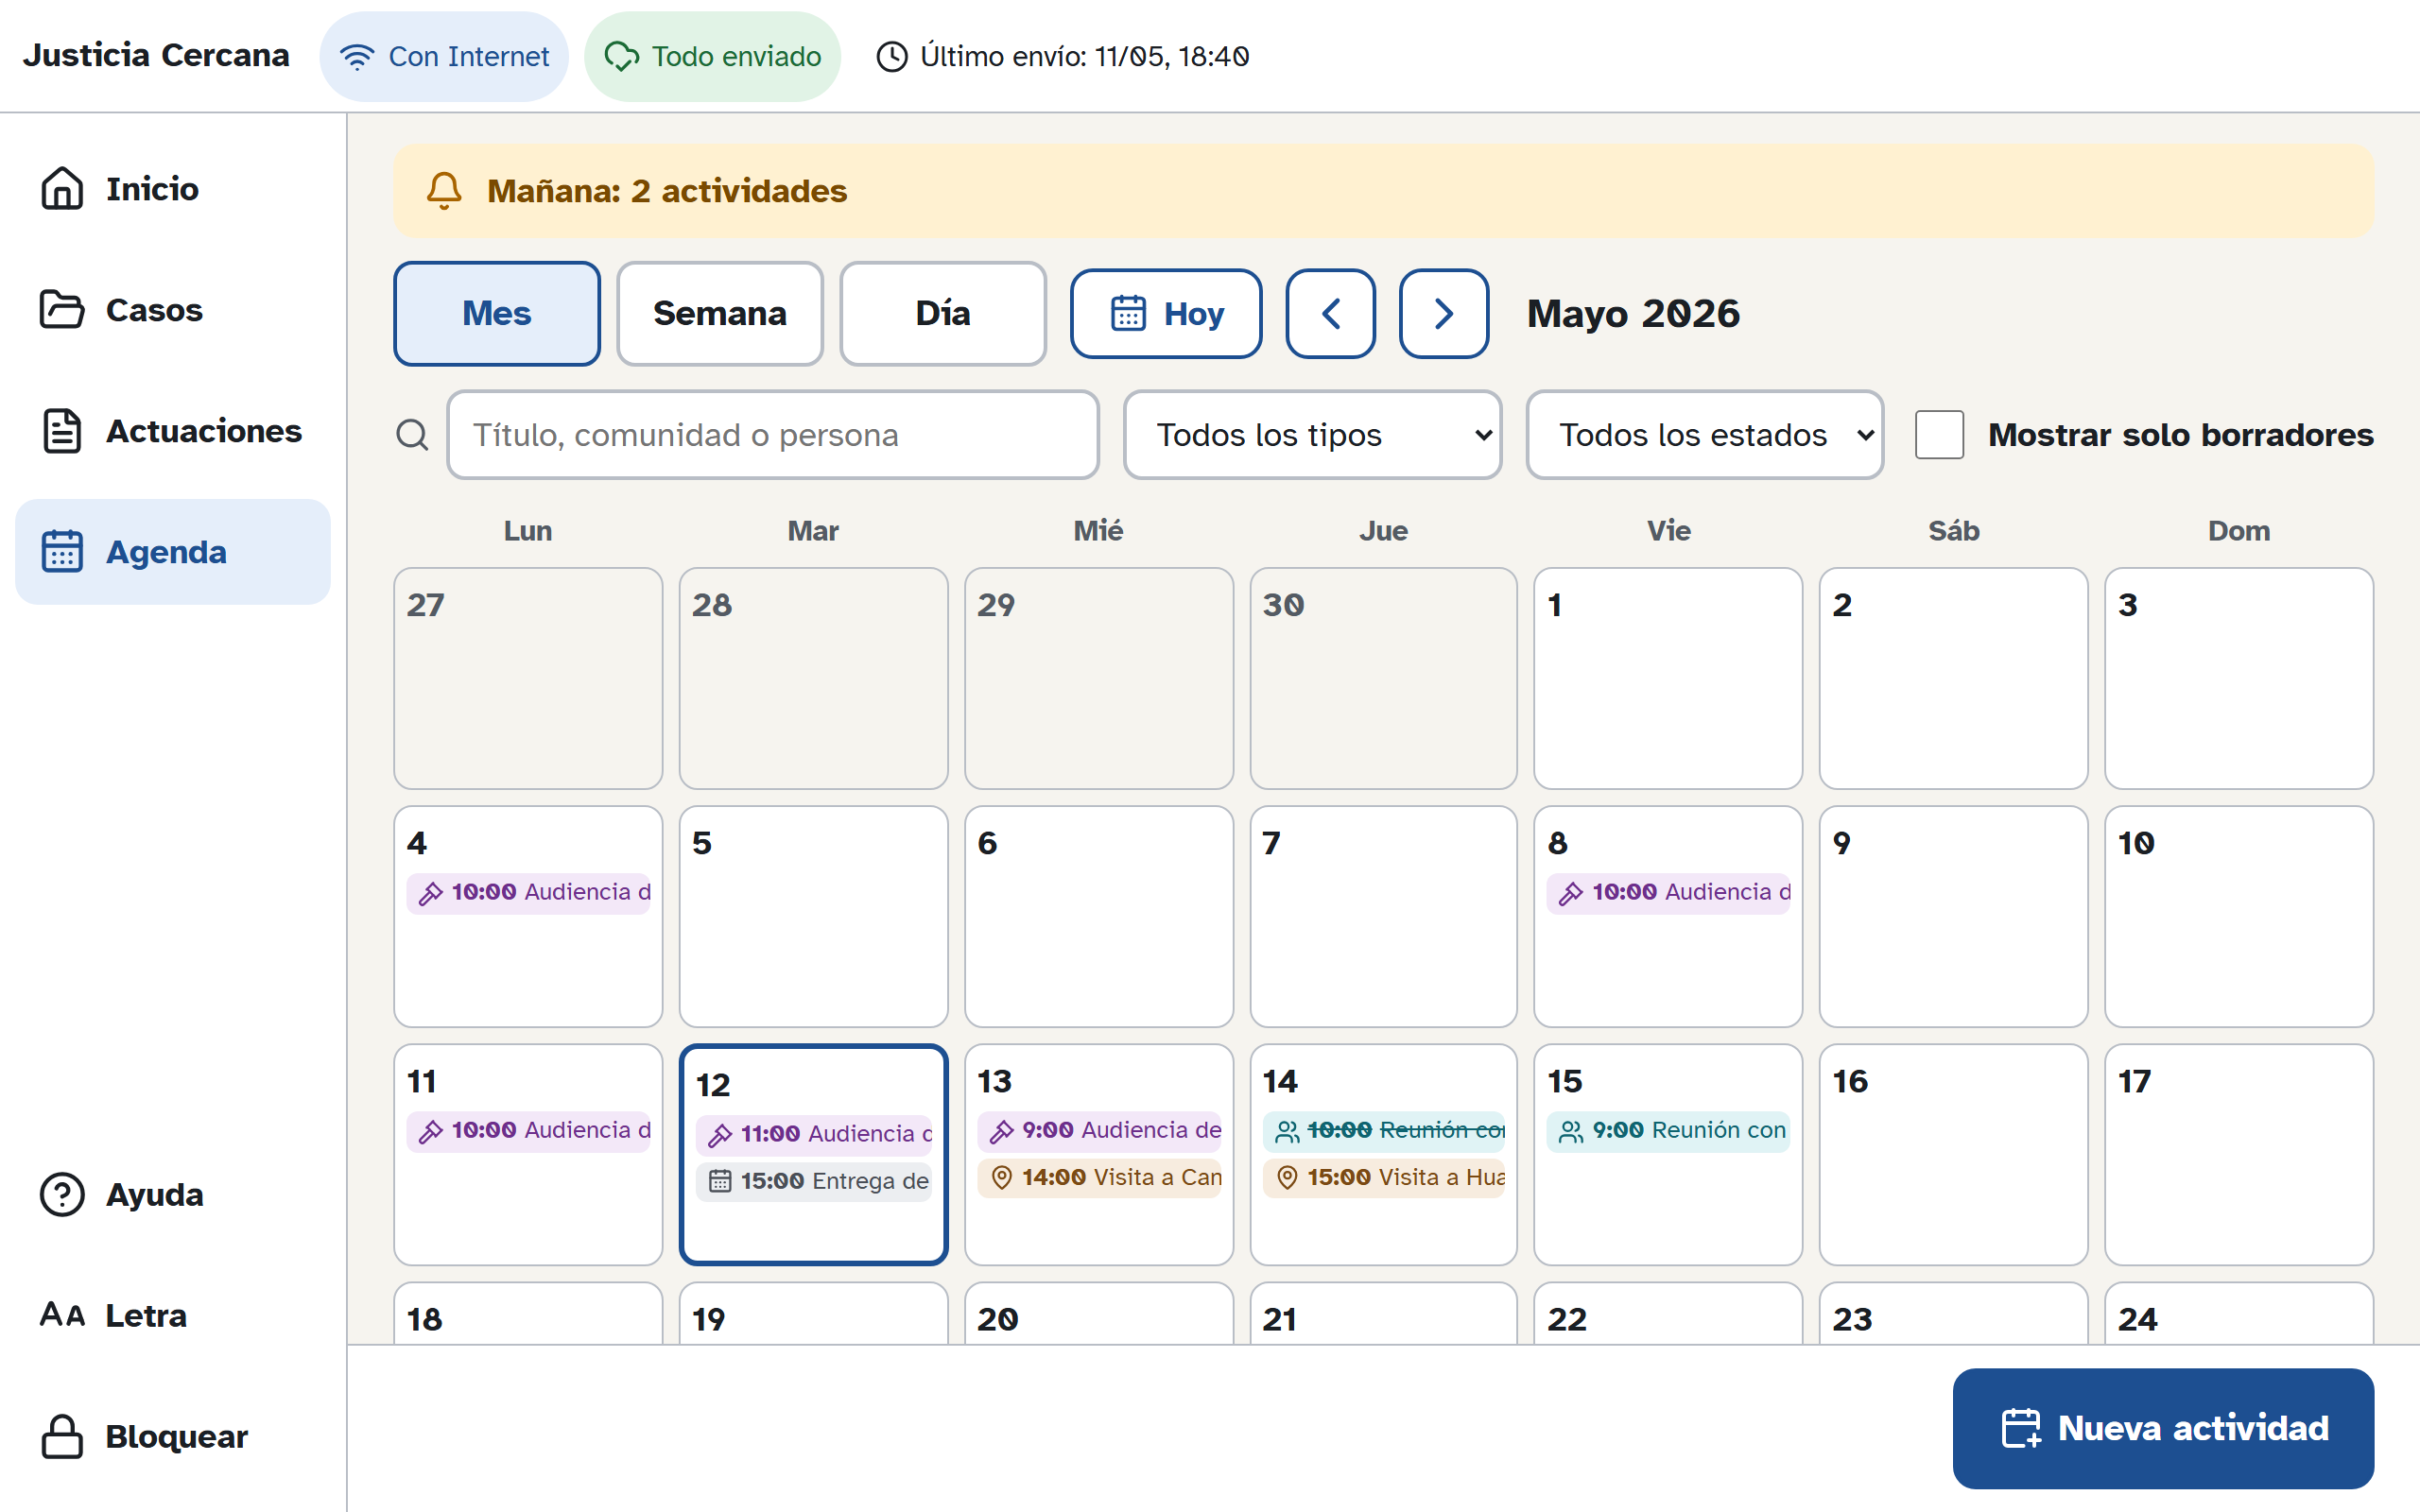
\includegraphics[width=\linewidth]{../../captures/P-07_agenda-mes.png}\\[-2pt]{\footnotesize\raggedright\textbf{P-07.} Agenda Mes: hasta 3 actividades por día y ``+2 más'' \emph{(Cobertura y funcionamiento de los módulos)}\par}\end{minipage}\hfill
\begin{minipage}[t]{0.49\textwidth}\centering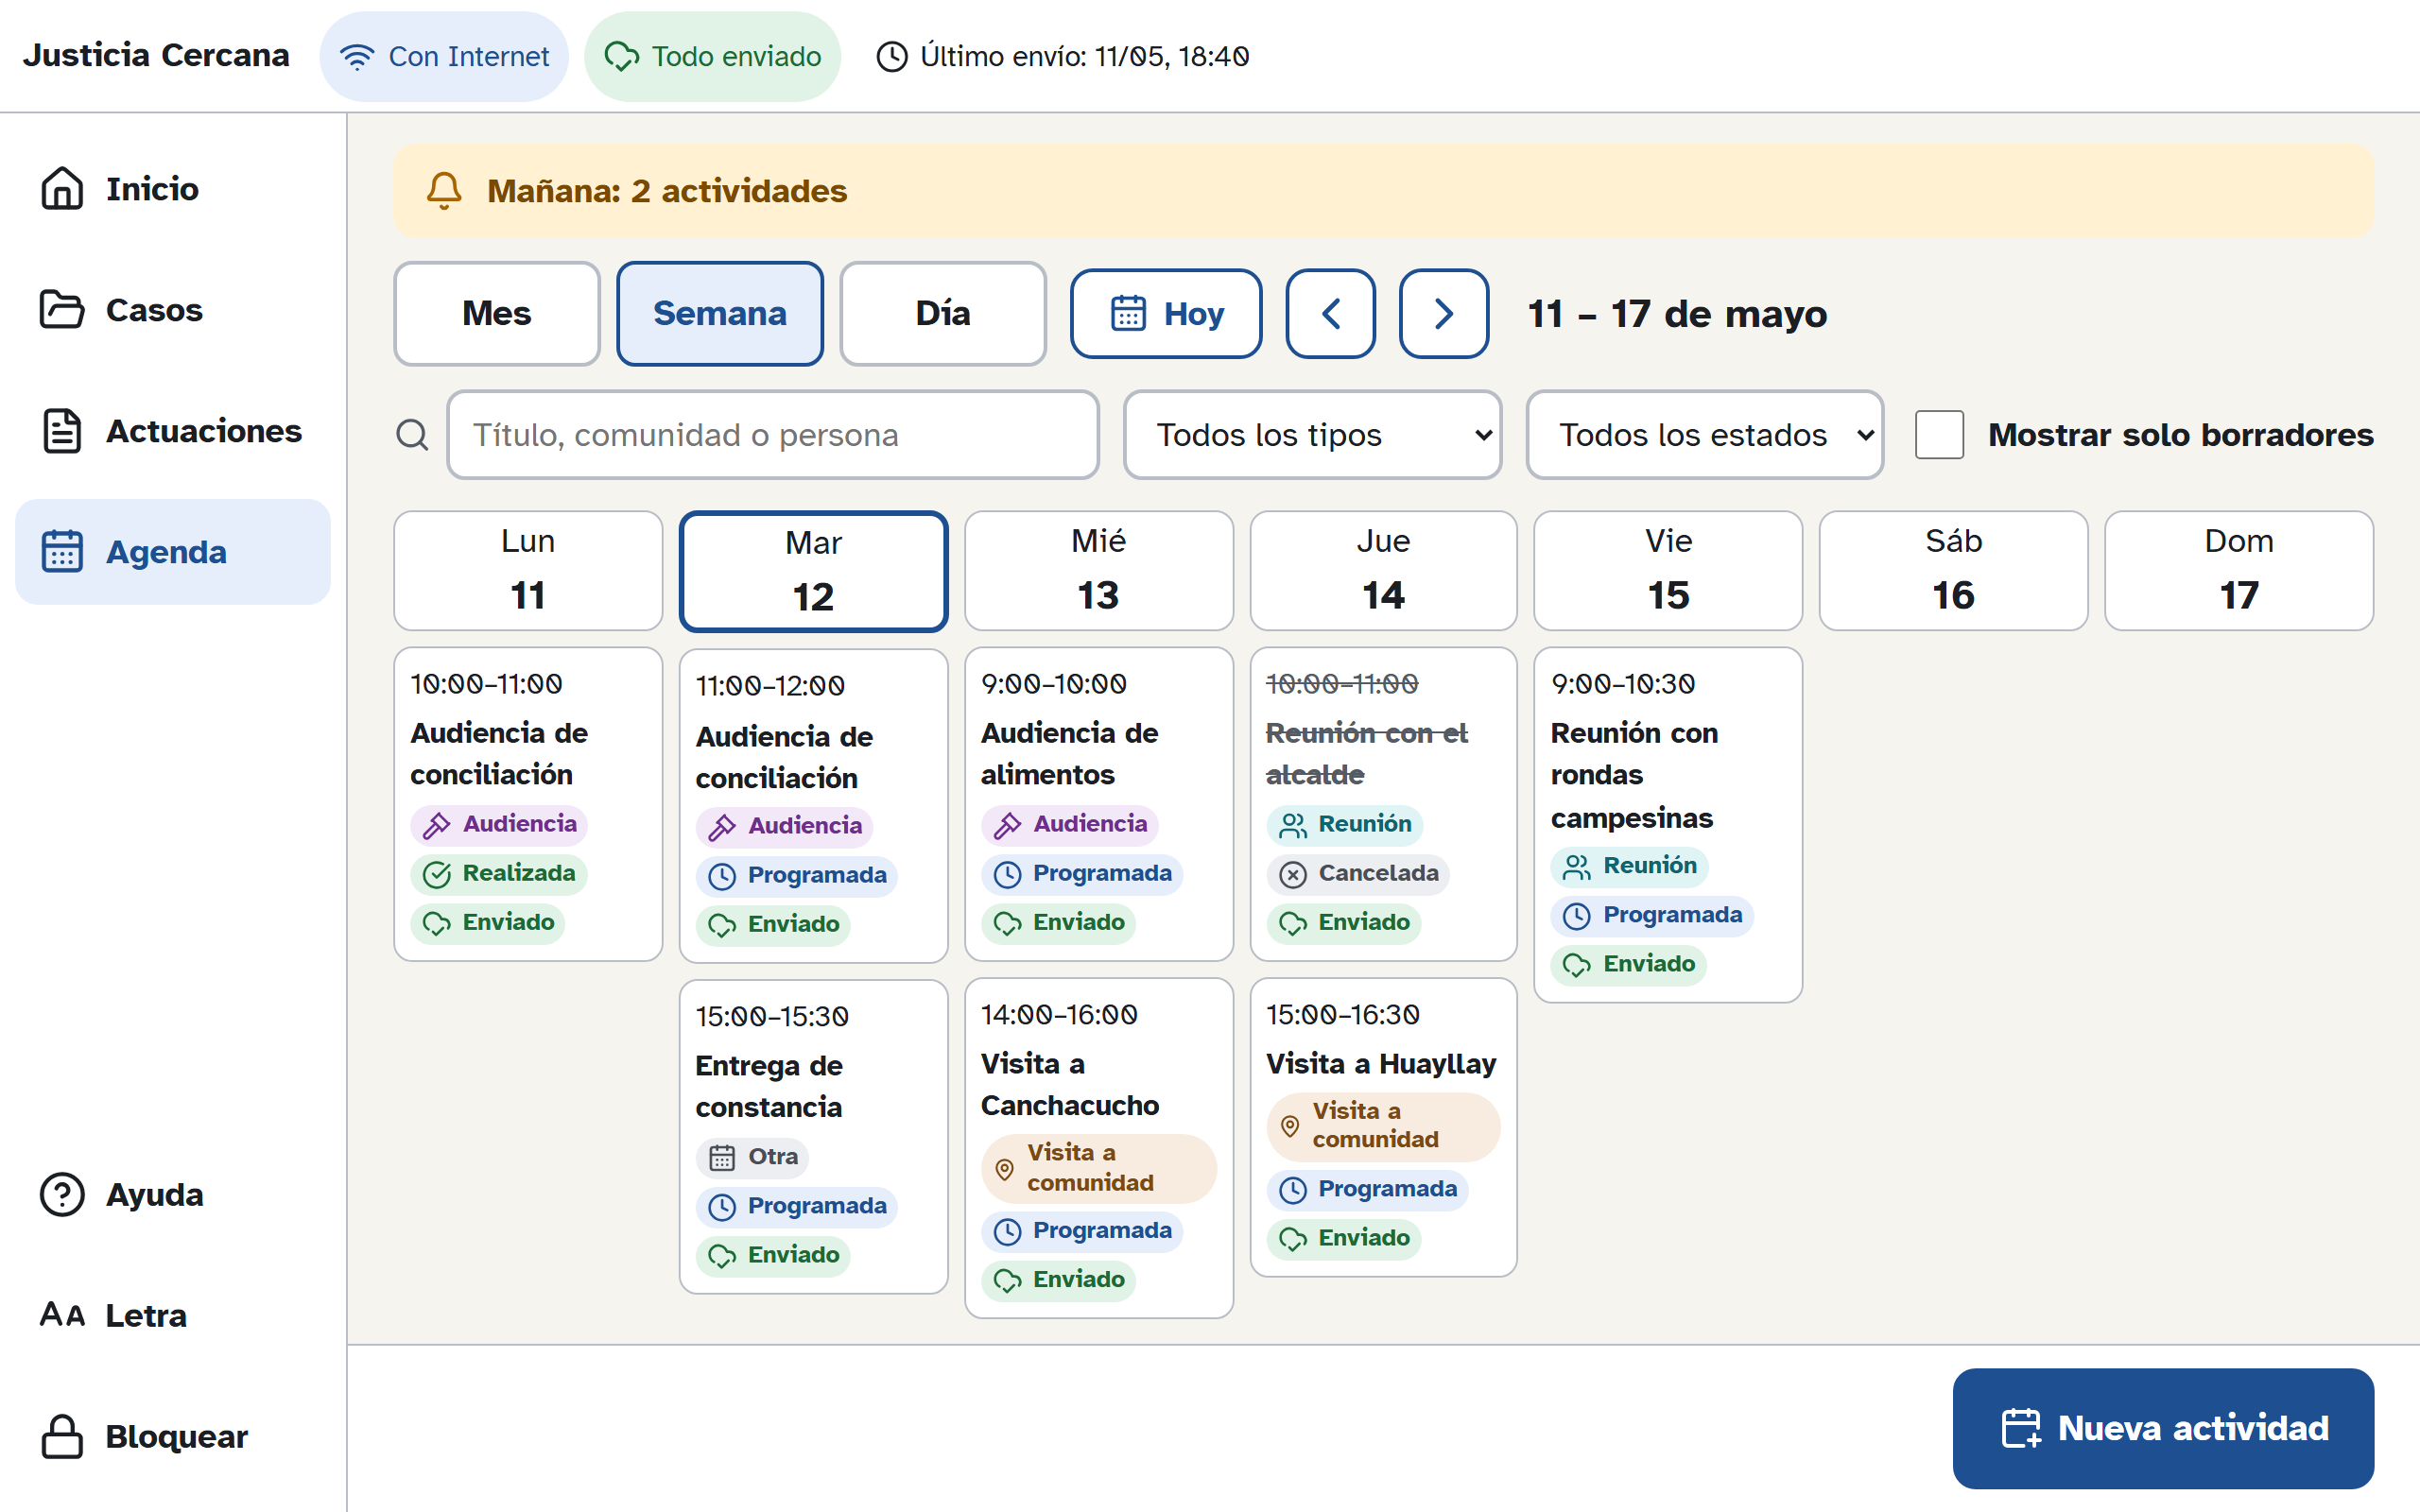
\includegraphics[width=\linewidth]{../../captures/P-07_agenda-semana.png}\\[-2pt]{\footnotesize\raggedright\textbf{P-07.} Agenda Semana: franja ``Mañana: 2 actividades'', categorías color + ícono + texto, estados \emph{(Cobertura y funcionamiento de los módulos)}\par}\end{minipage}\par\vspace{8pt}\noindent
\begin{minipage}[t]{0.49\textwidth}\centering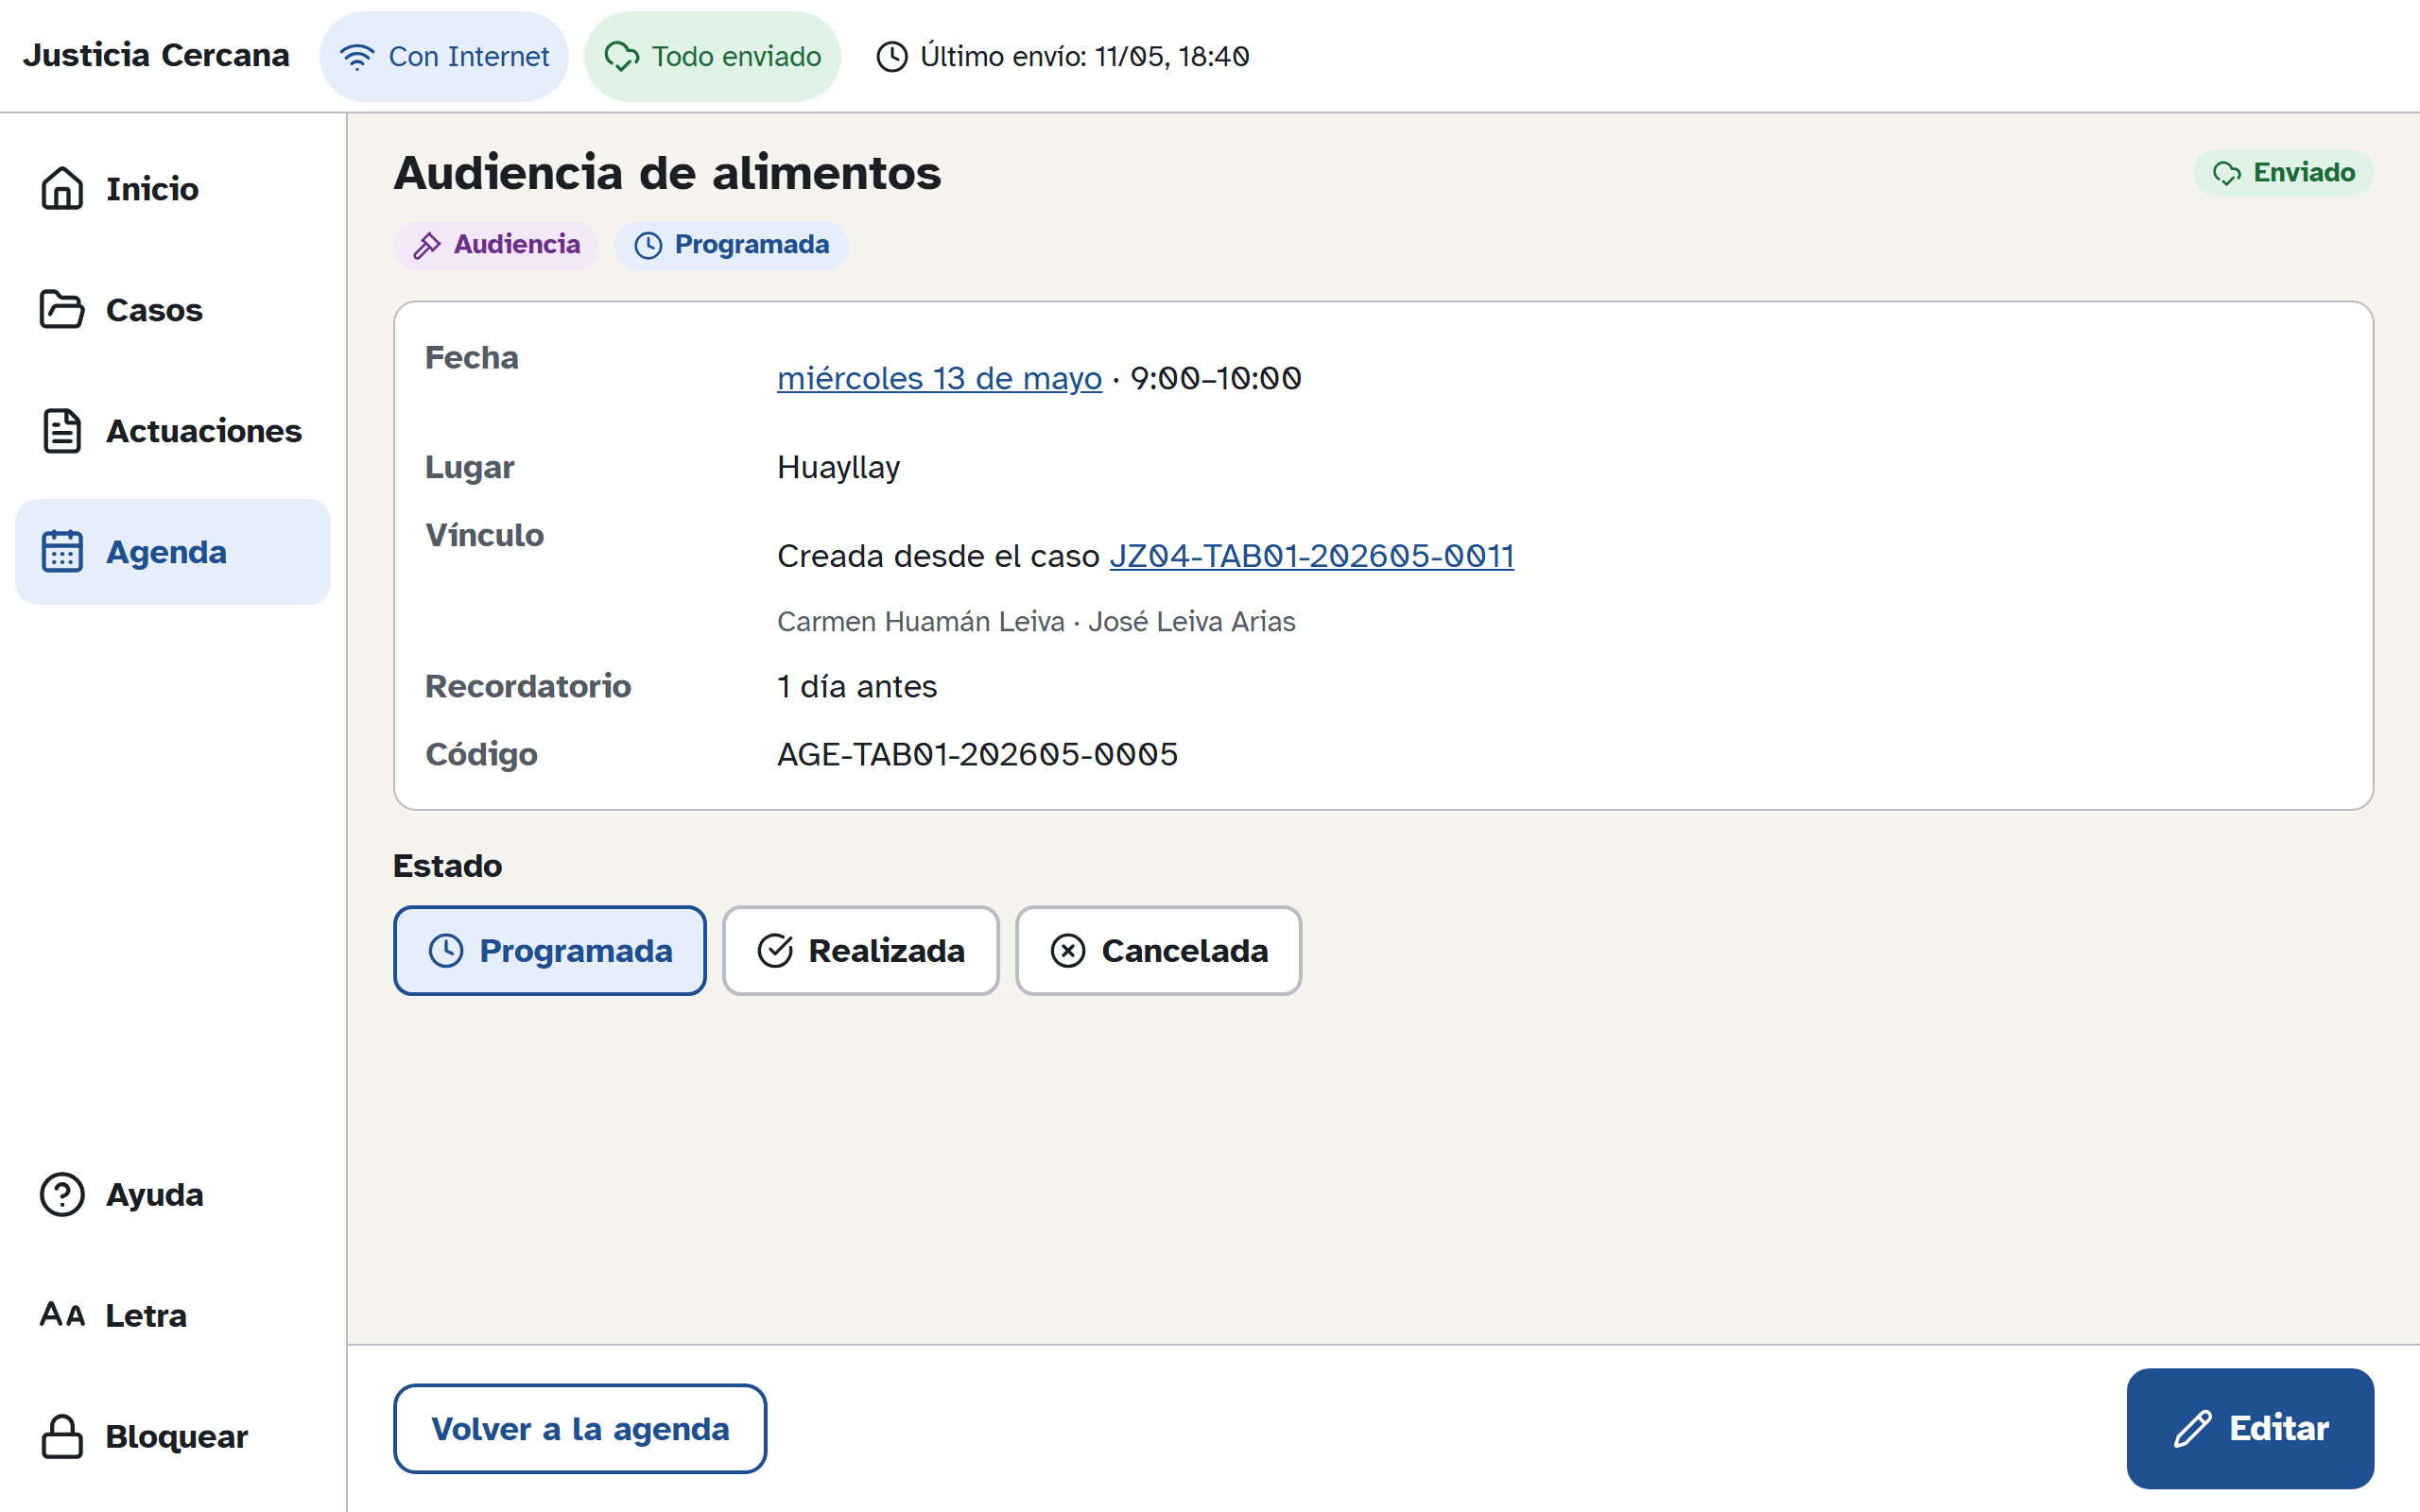
\includegraphics[width=\linewidth]{../../captures/P-08_actividad-detalle.png}\\[-2pt]{\footnotesize\raggedright\textbf{P-08.} Detalle de actividad: ``Creada desde el caso'' con enlace \emph{(Cobertura y funcionamiento de los módulos)}\par}\end{minipage}\hfill
\begin{minipage}[t]{0.49\textwidth}\centering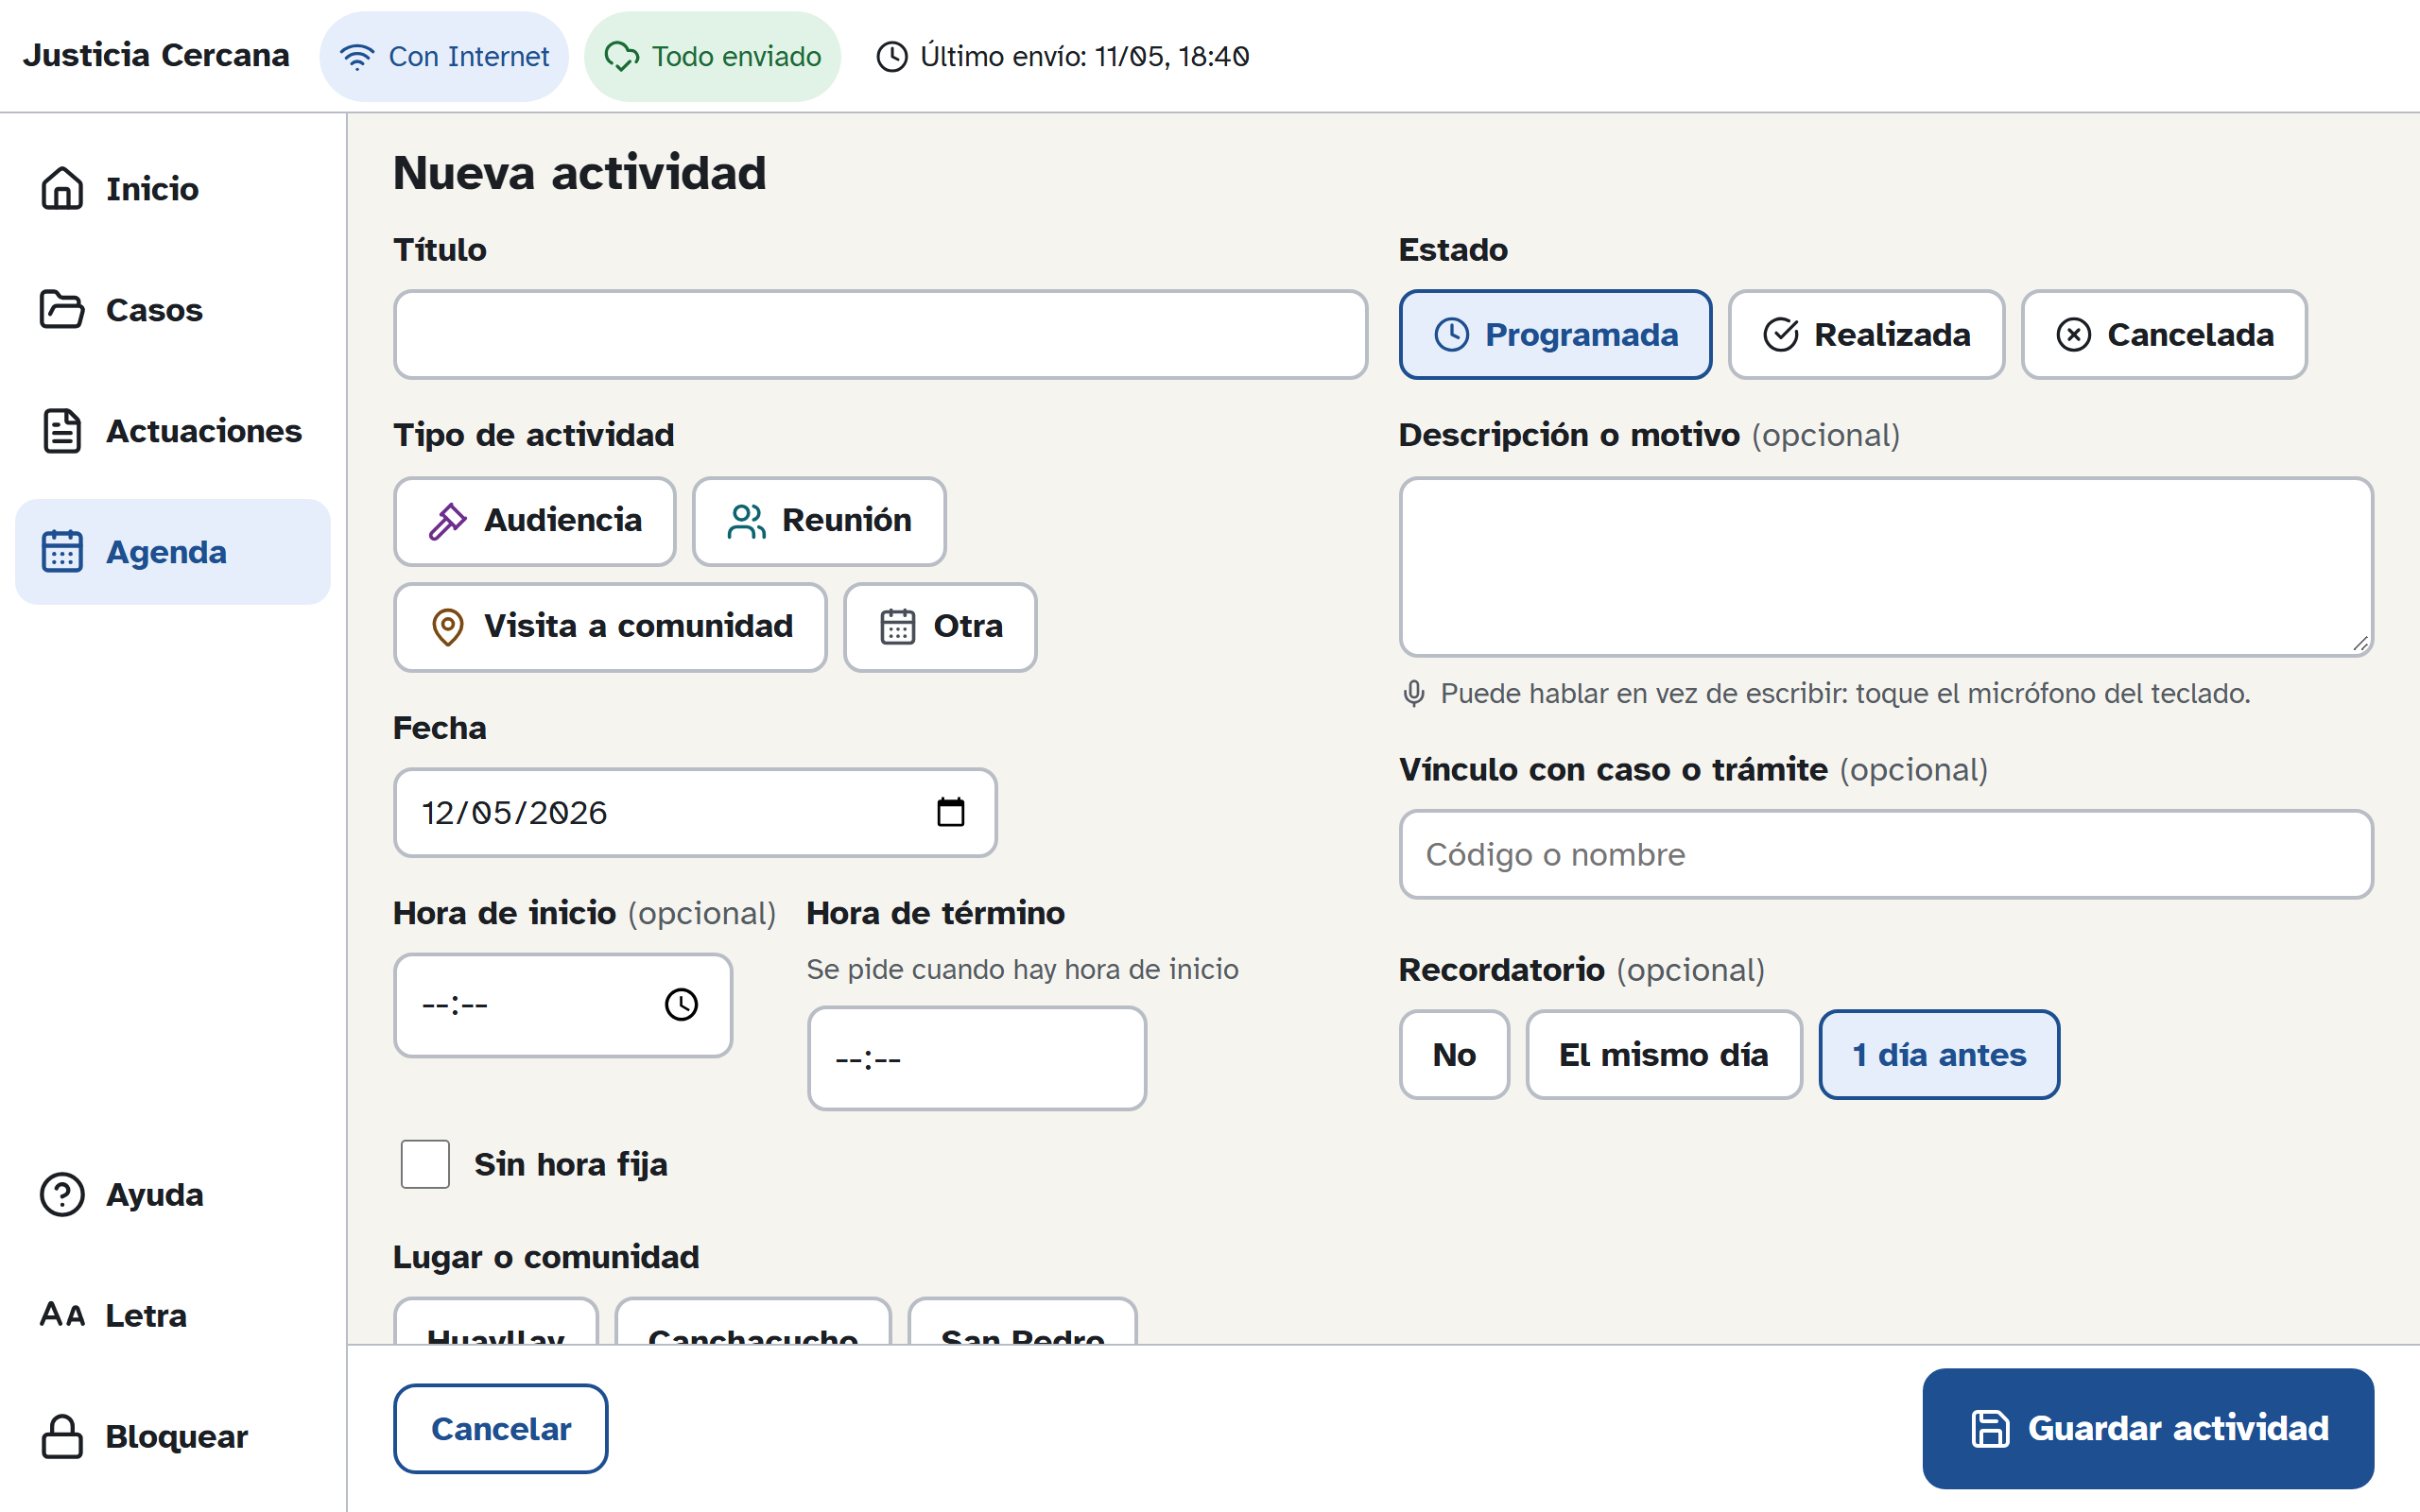
\includegraphics[width=\linewidth]{../../captures/P-08_actividad-nueva.png}\\[-2pt]{\footnotesize\raggedright\textbf{P-08.} Actividad nueva: todos los campos, ``(opcional)'', condicional de hora de término \emph{(Cobertura y funcionamiento de los módulos)}\par}\end{minipage}\par\vspace{8pt}\noindent
\begin{minipage}[t]{0.49\textwidth}\centering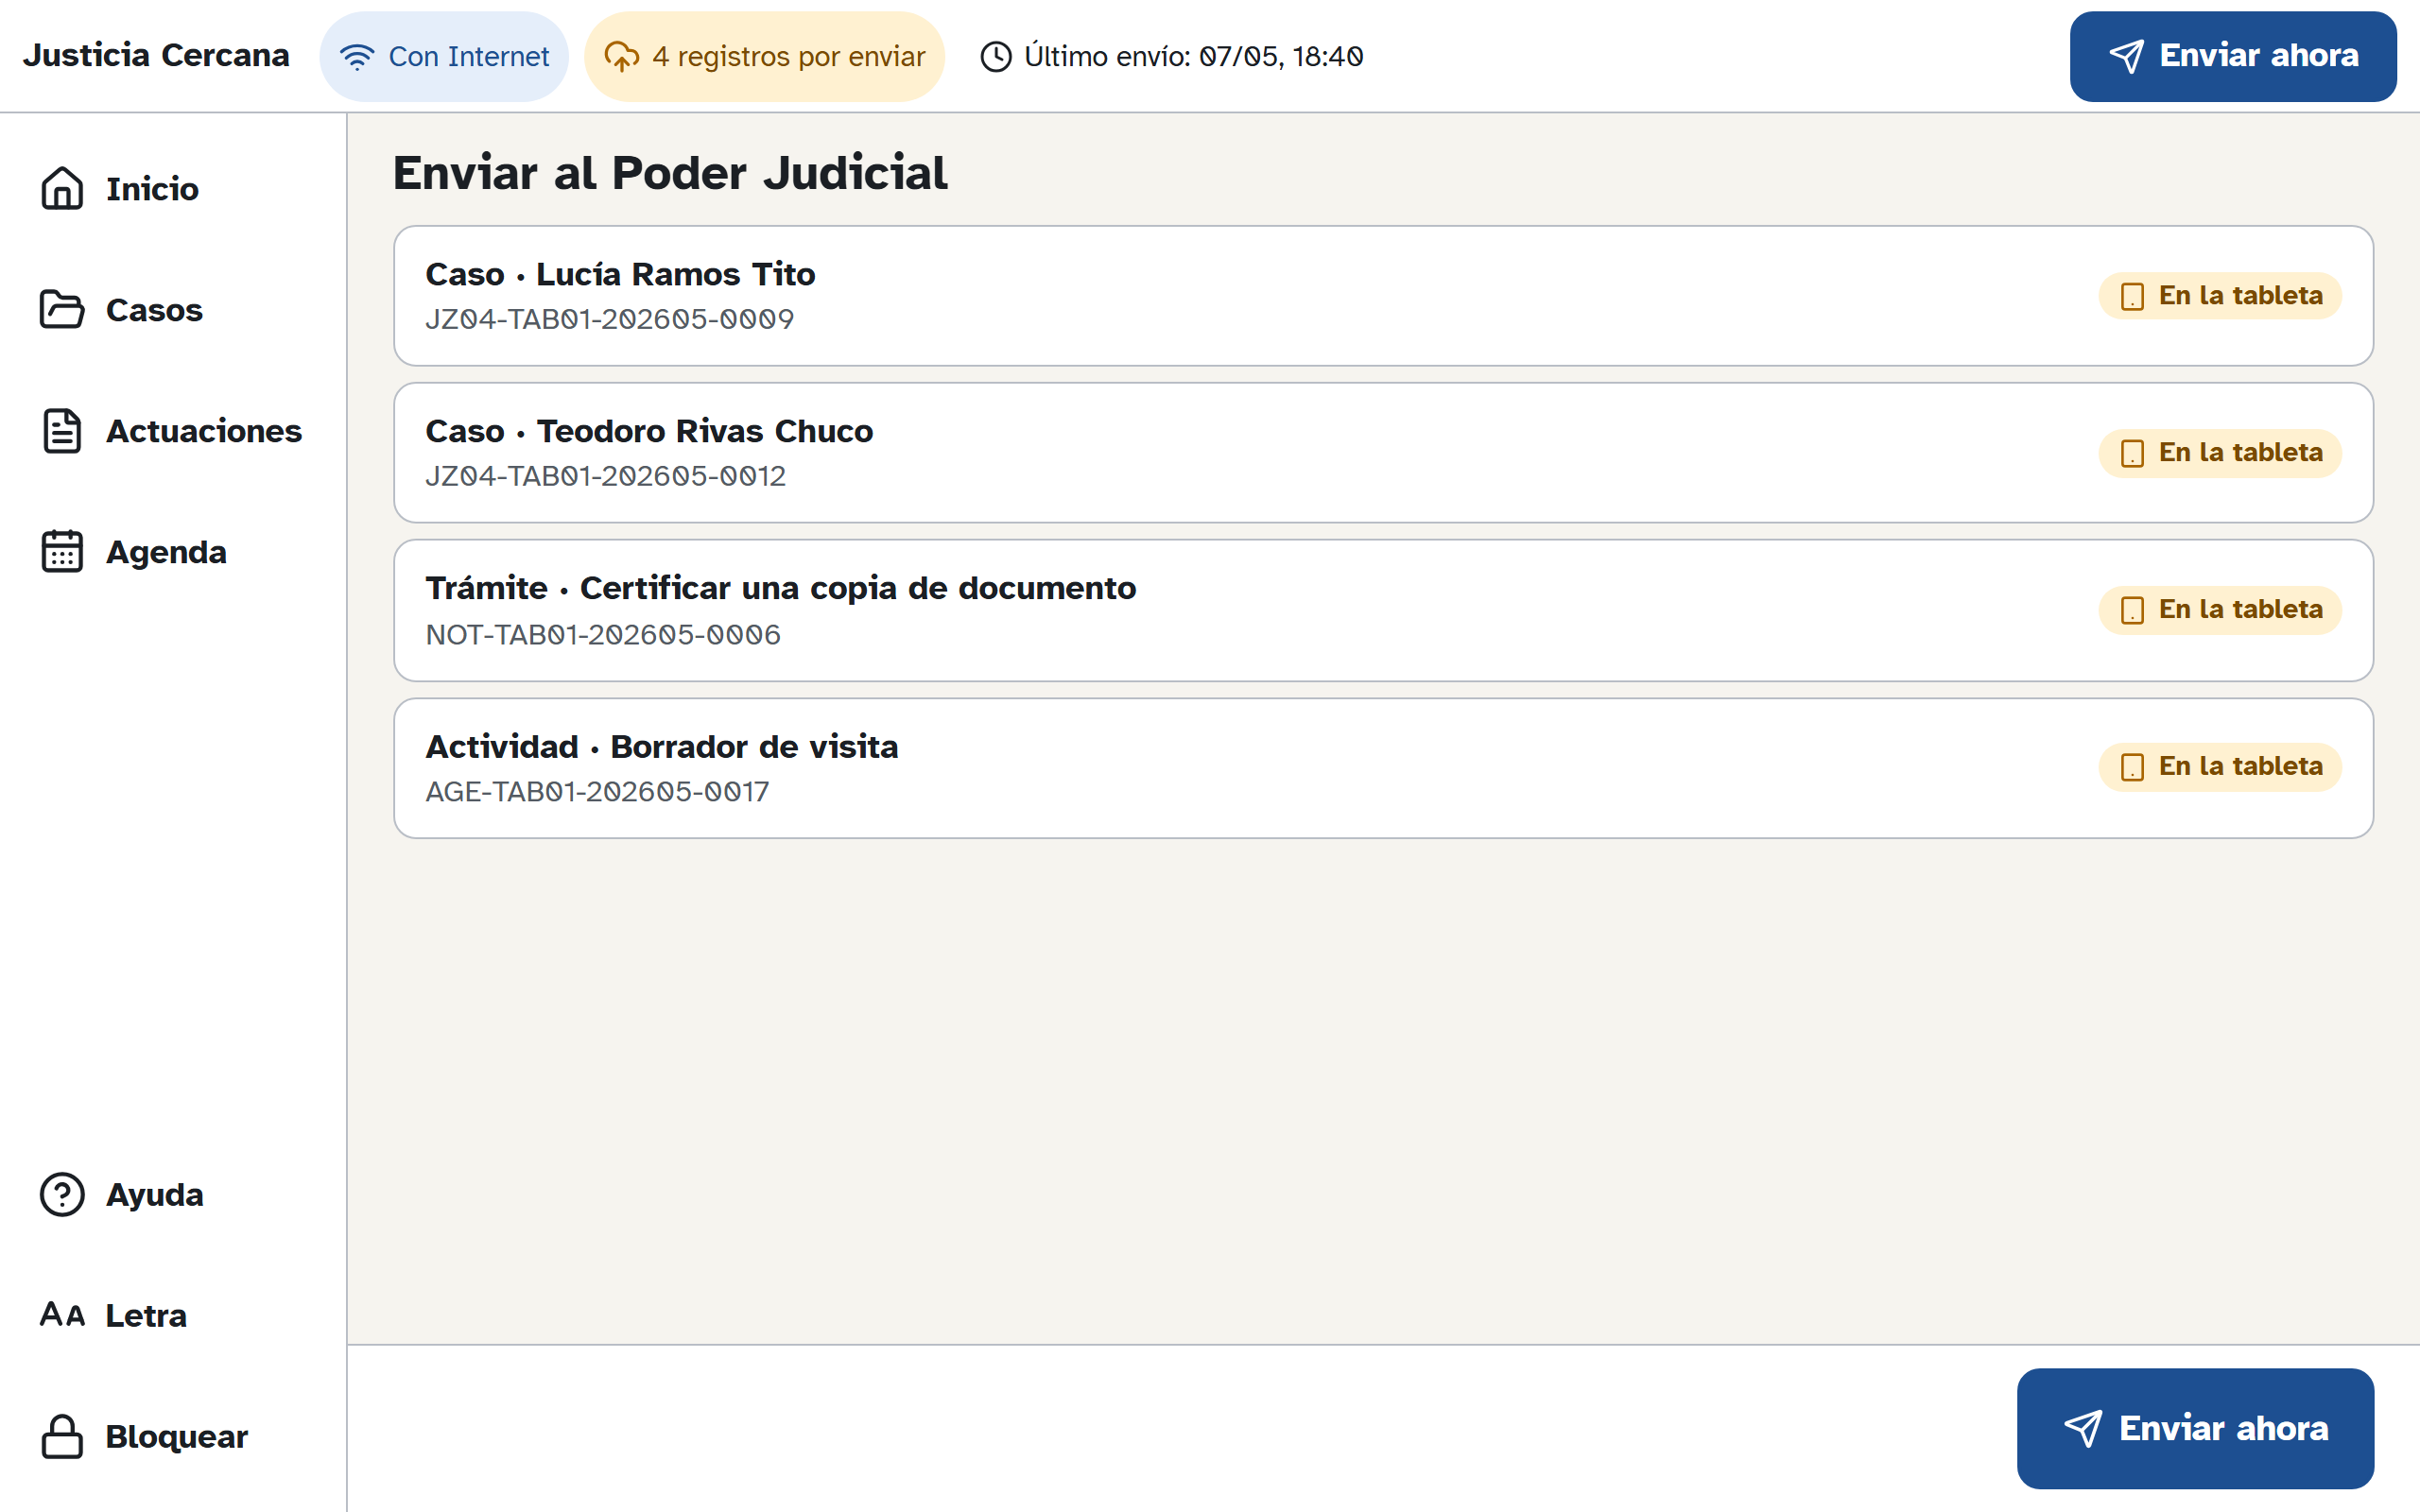
\includegraphics[width=\linewidth]{../../captures/P-09_envio.png}\\[-2pt]{\footnotesize\raggedright\textbf{P-09.} Envío al Poder Judicial: registros por enviar con distintivo y [Enviar ahora] \emph{(Funcionamiento sin conexión)}\par}\end{minipage}\hfill
\begin{minipage}[t]{0.49\textwidth}\centering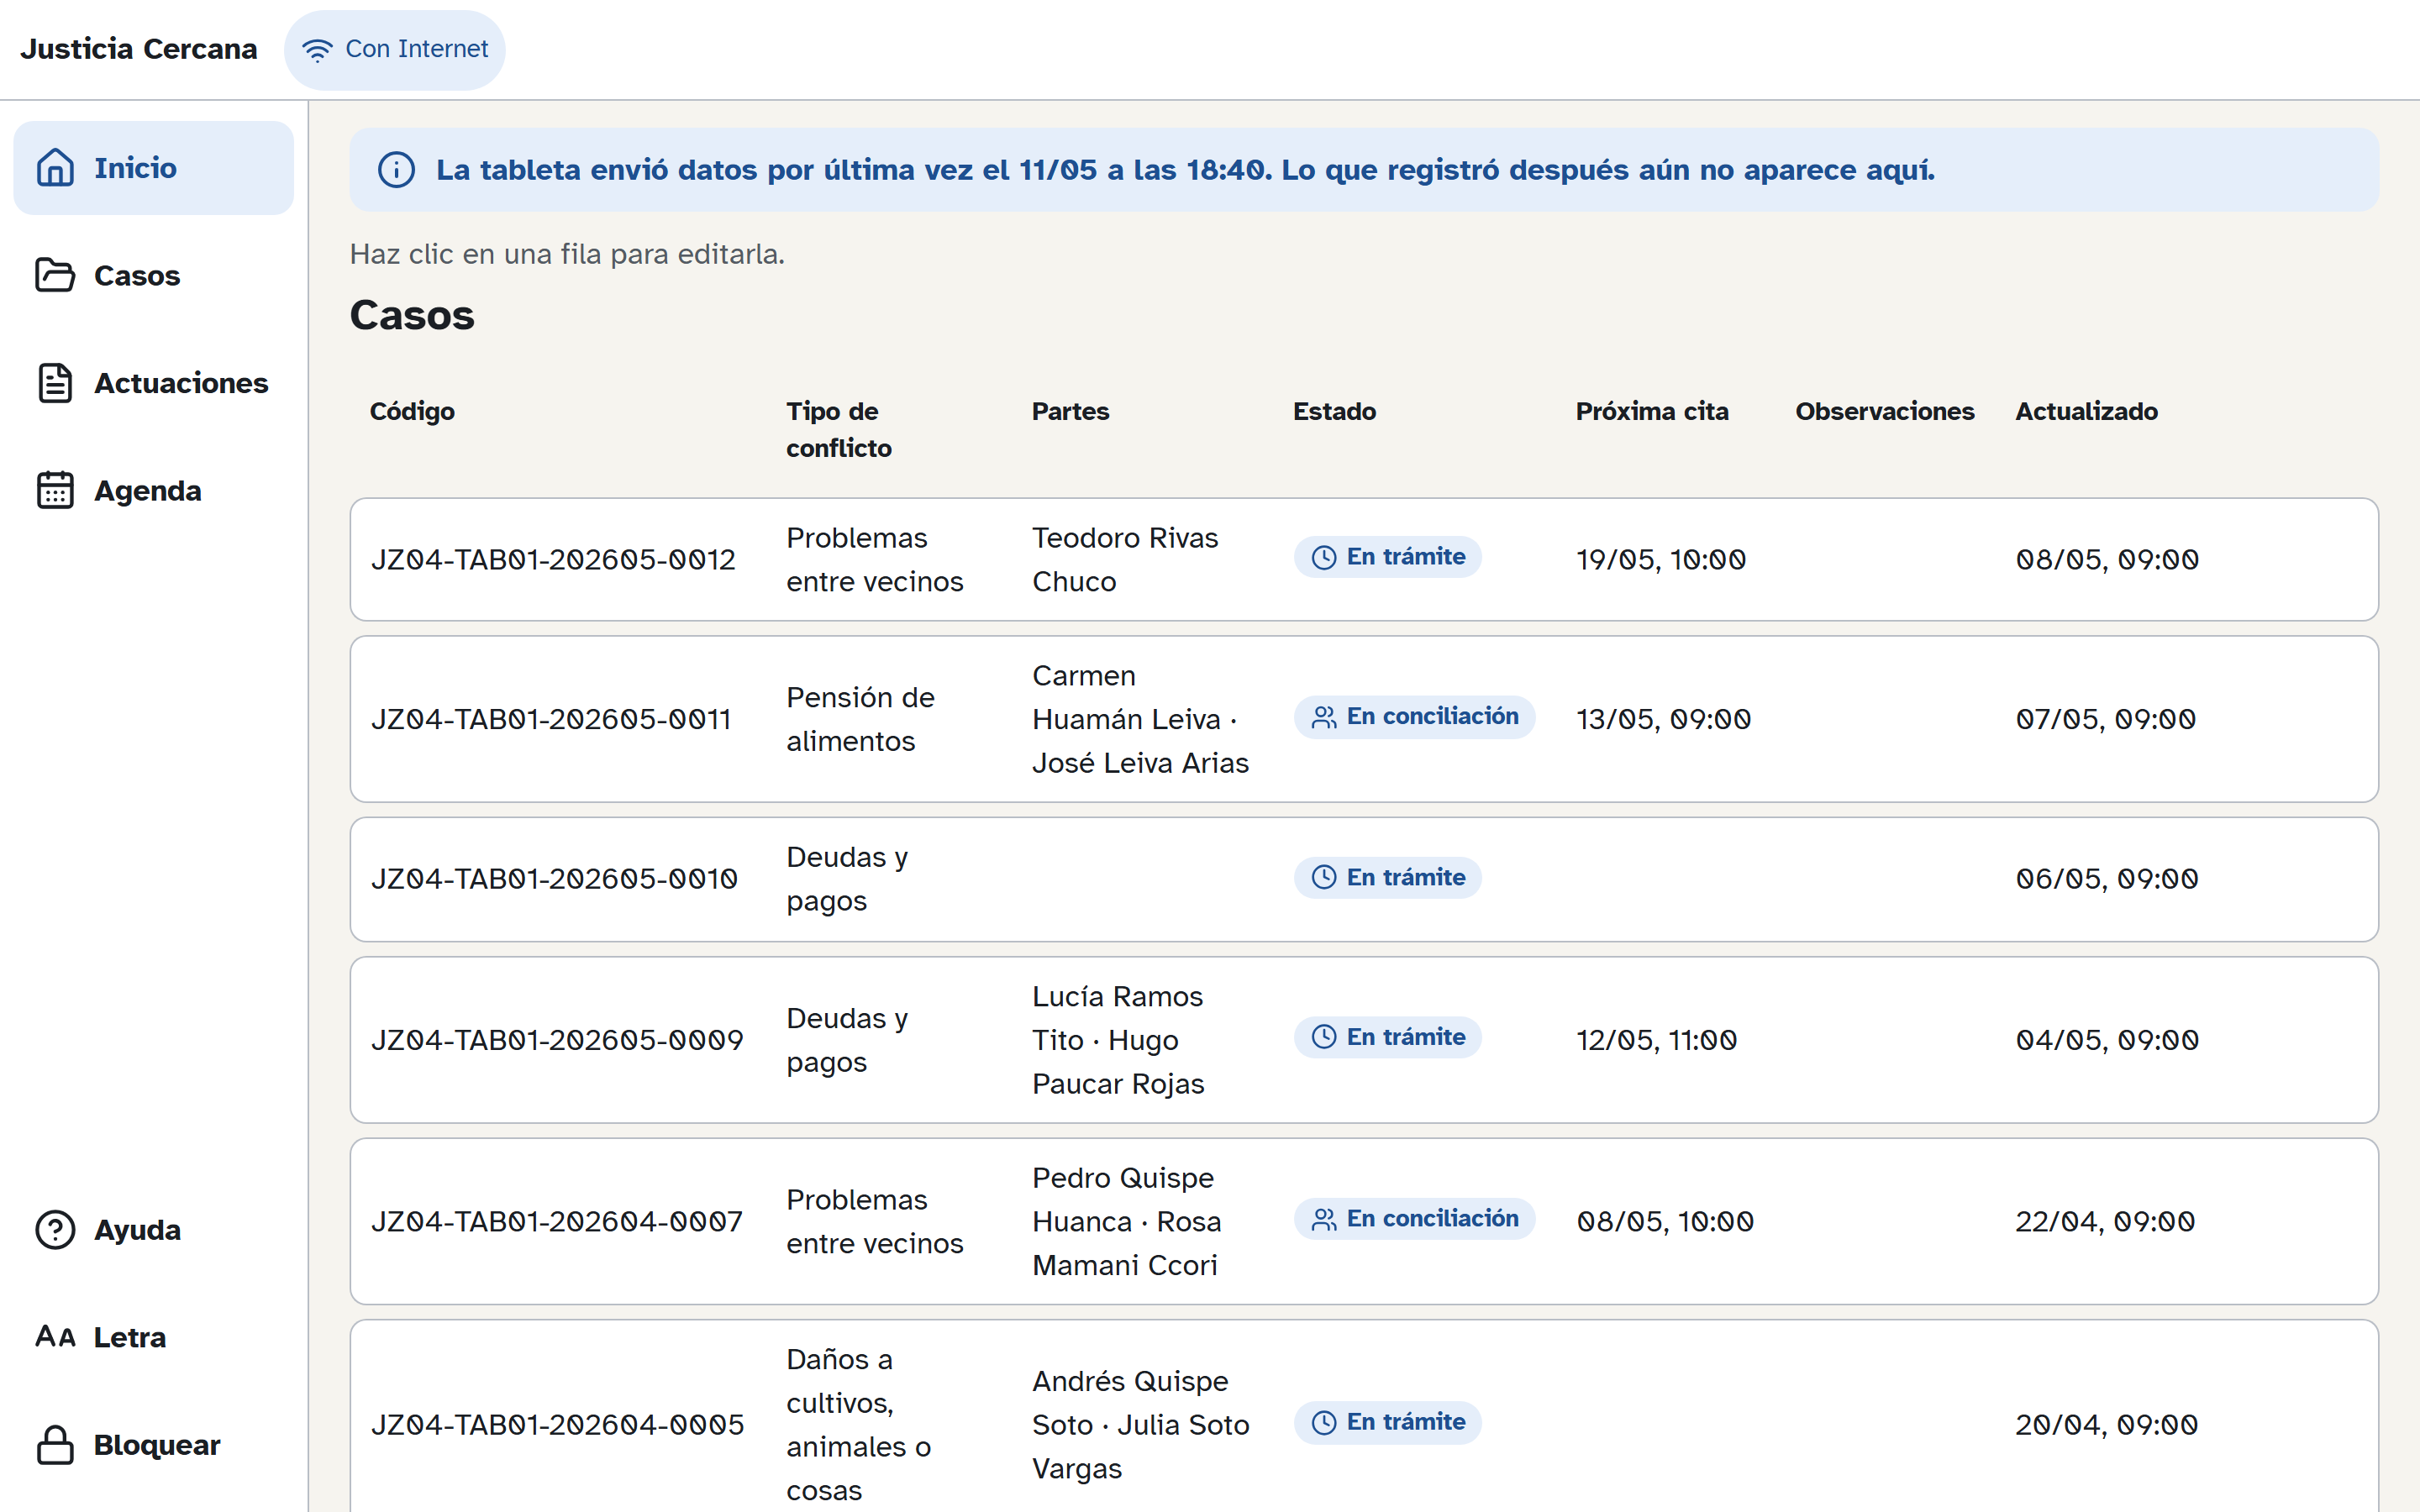
\includegraphics[width=\linewidth]{../../captures/P-10_computadora.png}\\[-2pt]{\footnotesize\raggedright\textbf{P-10.} Vista en computadora 1440×900: tablas con más columnas, aviso del último envío \emph{(Cobertura y funcionamiento de los módulos)}\par}\end{minipage}\par\vspace{8pt}\noindent
\par\vspace{4pt}
\subsection*{Flujo 1}
\noindent
\begin{minipage}[t]{0.49\textwidth}\centering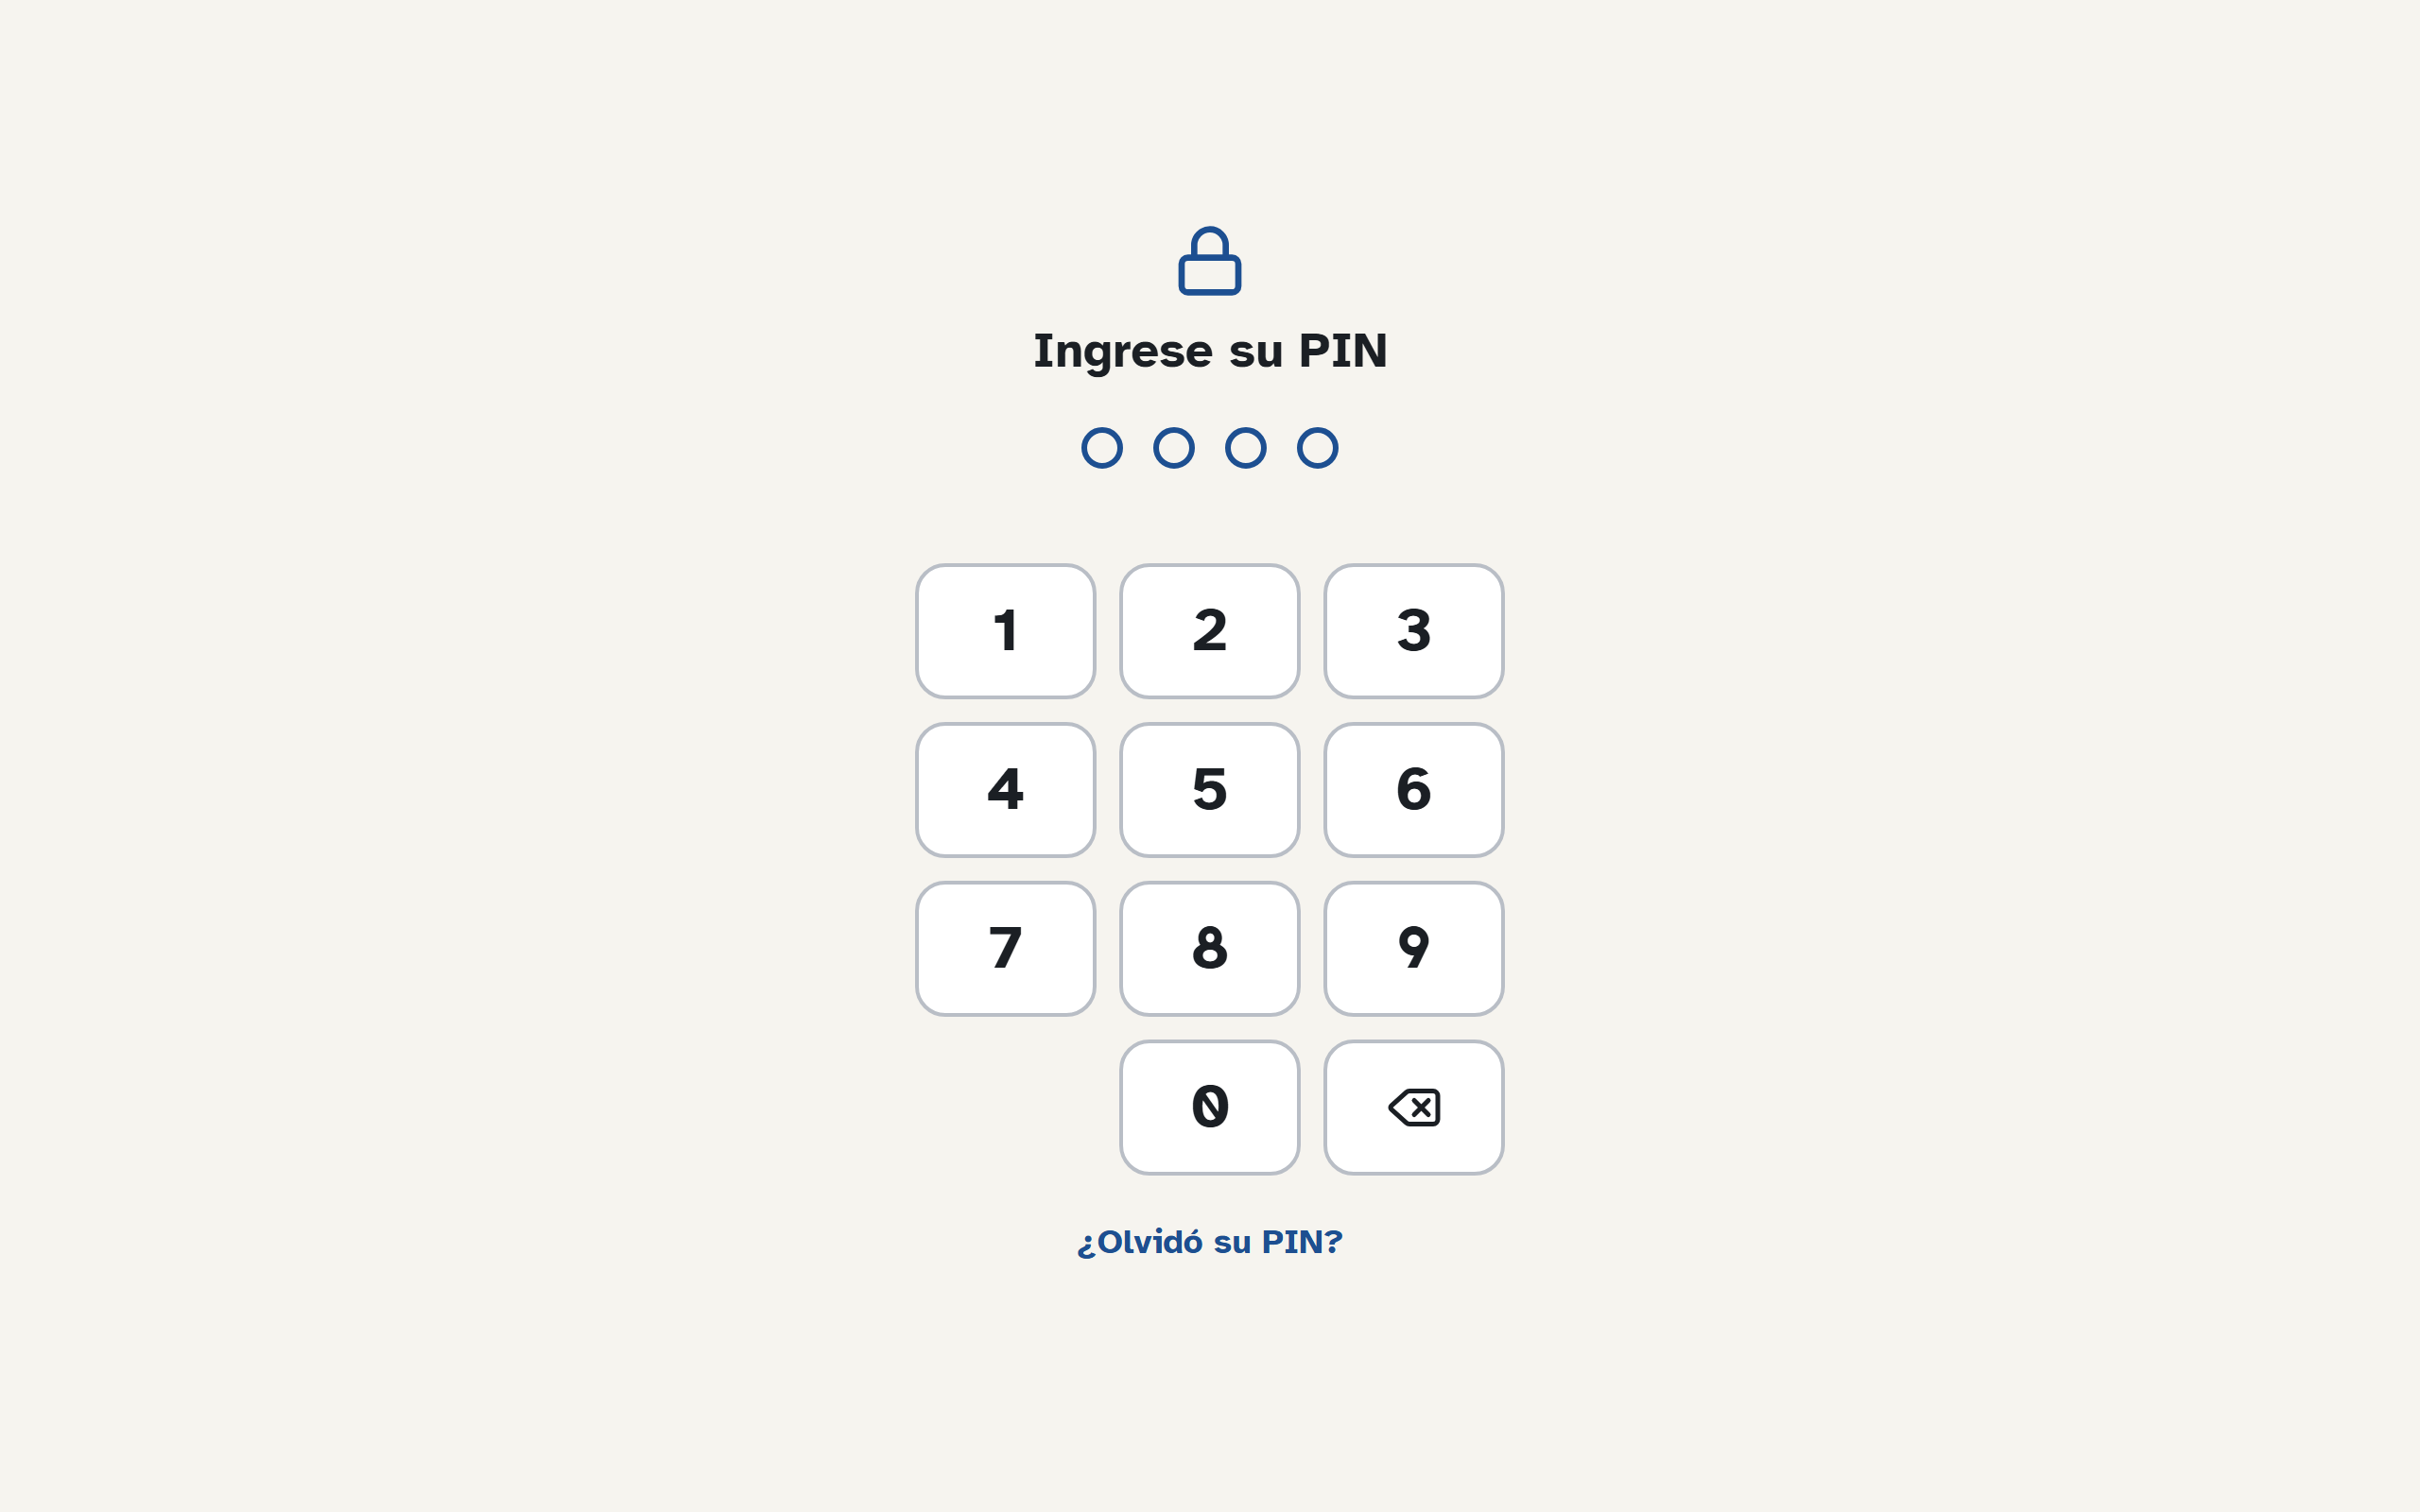
\includegraphics[width=\linewidth]{../../captures/F1-01a_pin.png}\\[-2pt]{\footnotesize\raggedright\textbf{P-00 · 1.} Ingreso con PIN numérico y teclado grande; funciona sin Internet \emph{(Factores humanos y dispositivo)}\par}\end{minipage}\hfill
\begin{minipage}[t]{0.49\textwidth}\centering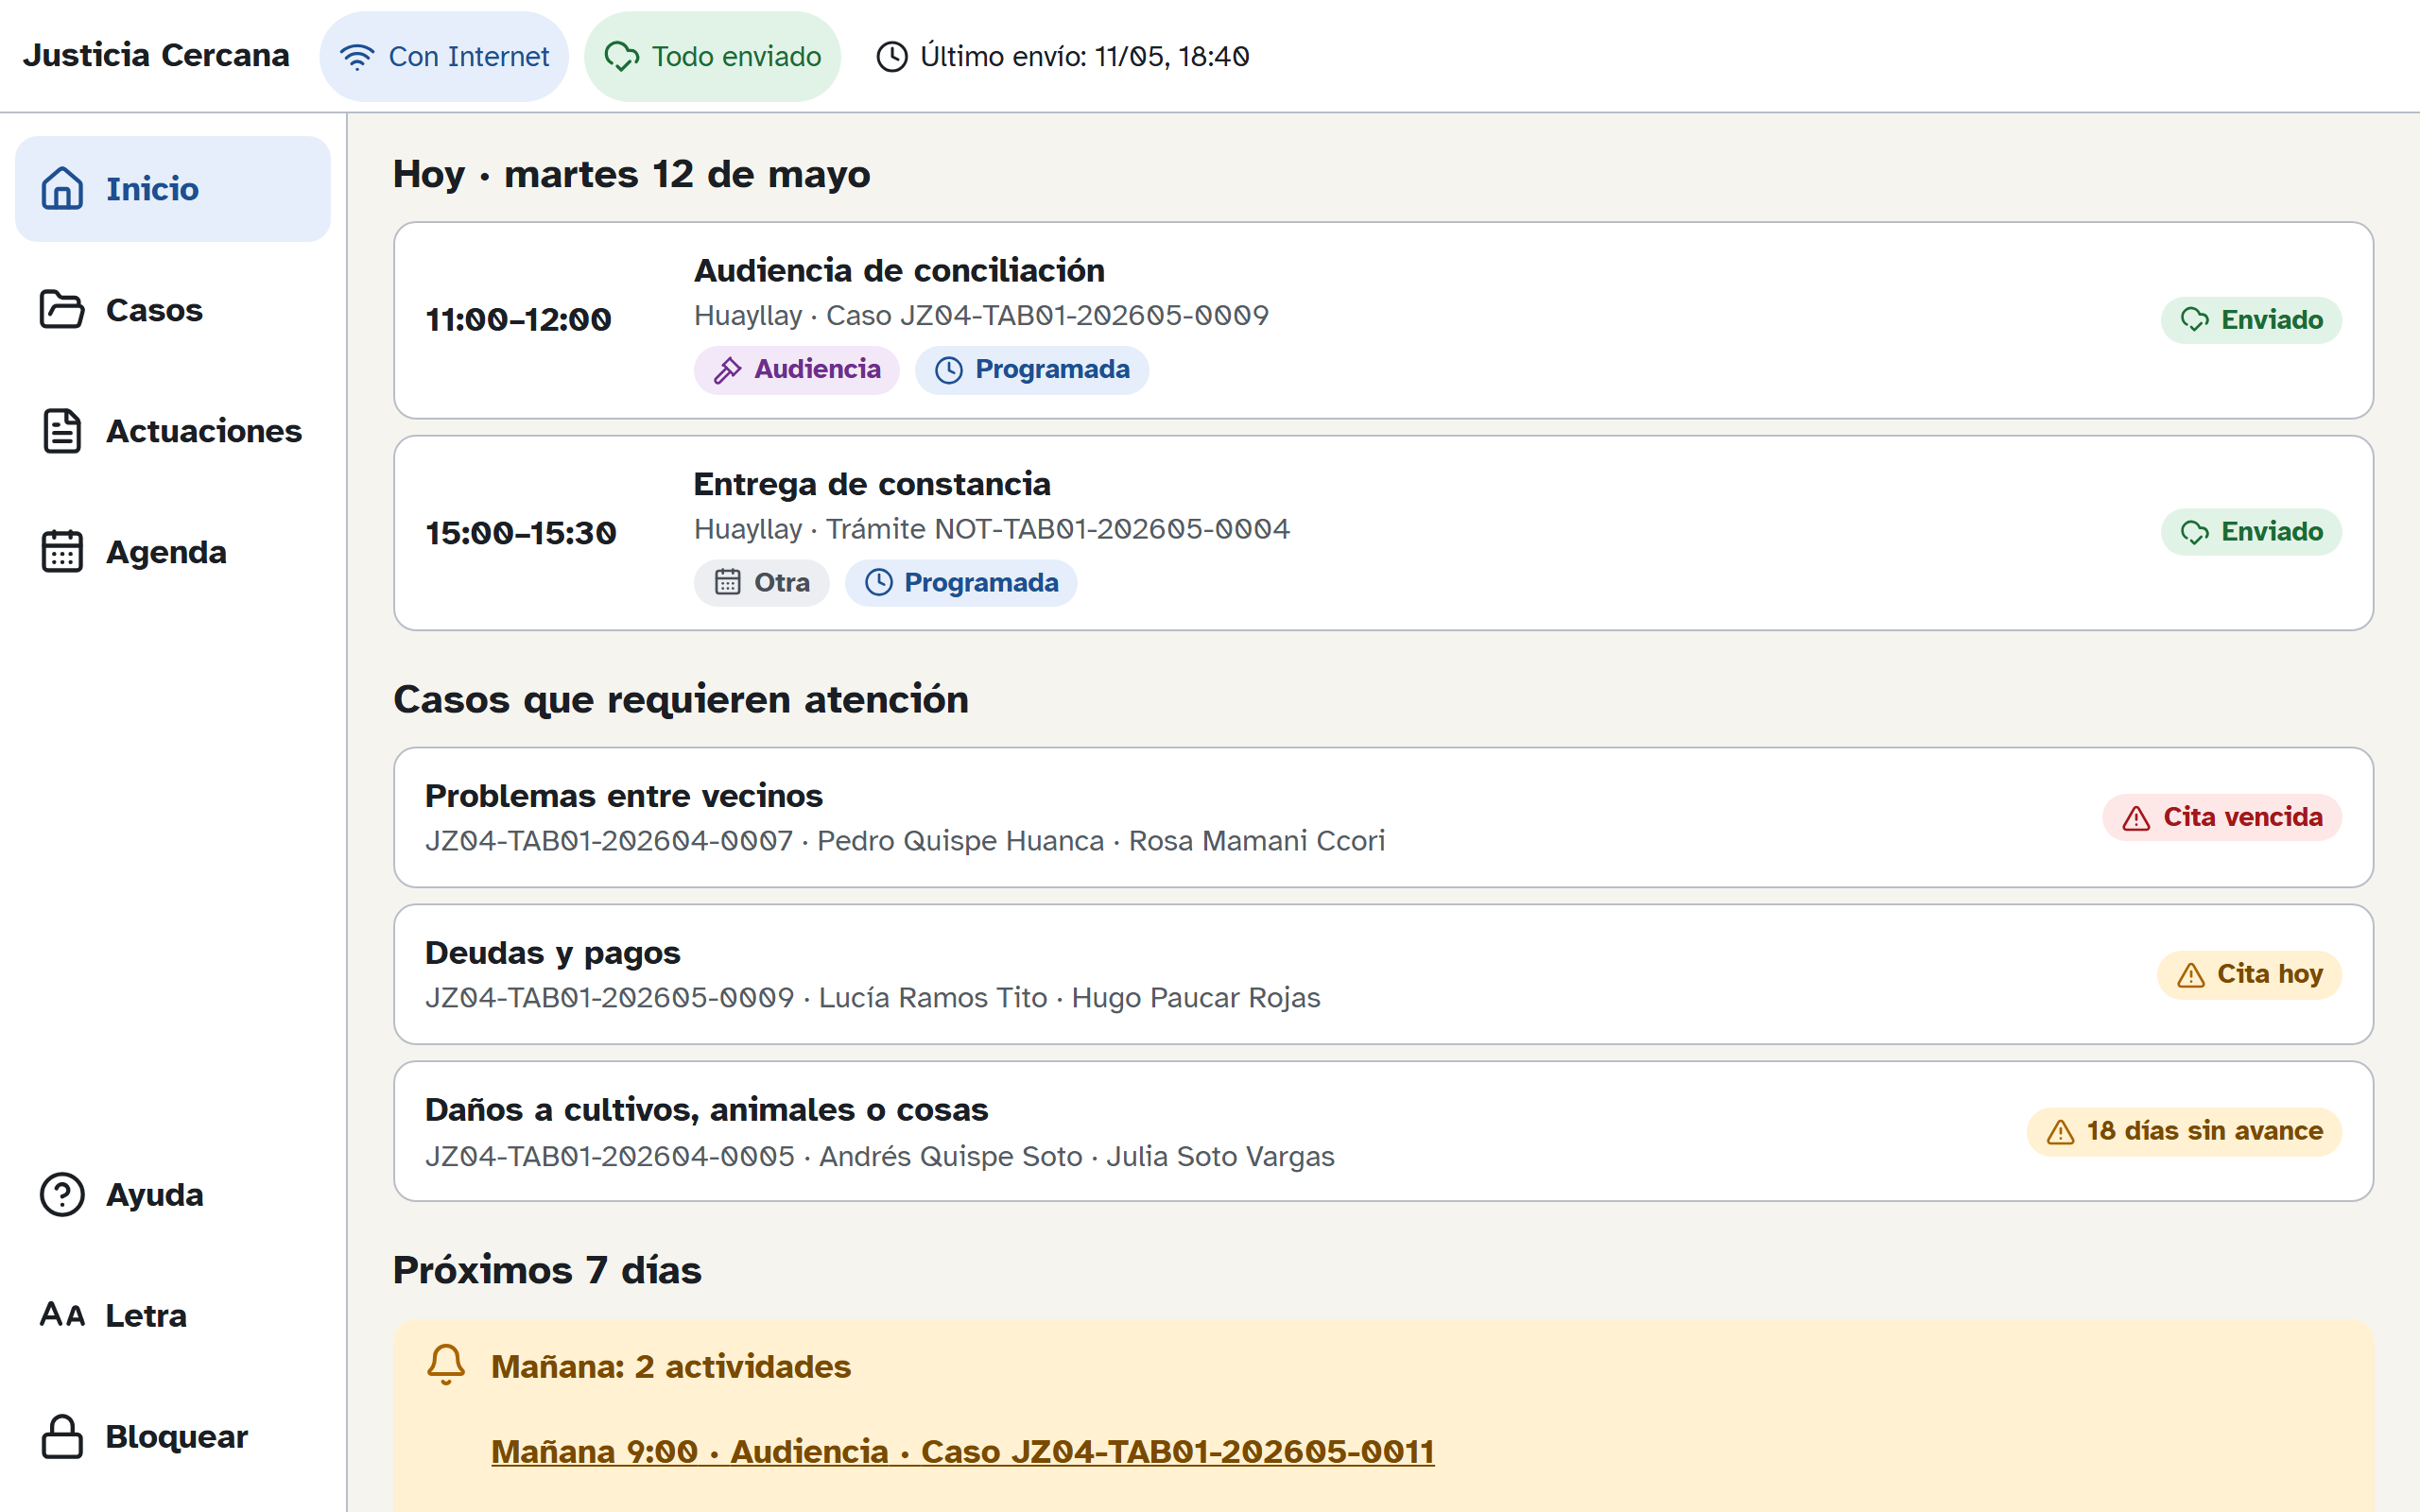
\includegraphics[width=\linewidth]{../../captures/F1-01b_inicio-con-internet.png}\\[-2pt]{\footnotesize\raggedright\textbf{P-01 · 1.} Inicio con barra ``Con Internet'' · ``Todo enviado'' \emph{(Funcionamiento sin conexión)}\par}\end{minipage}\par\vspace{8pt}\noindent
\begin{minipage}[t]{0.49\textwidth}\centering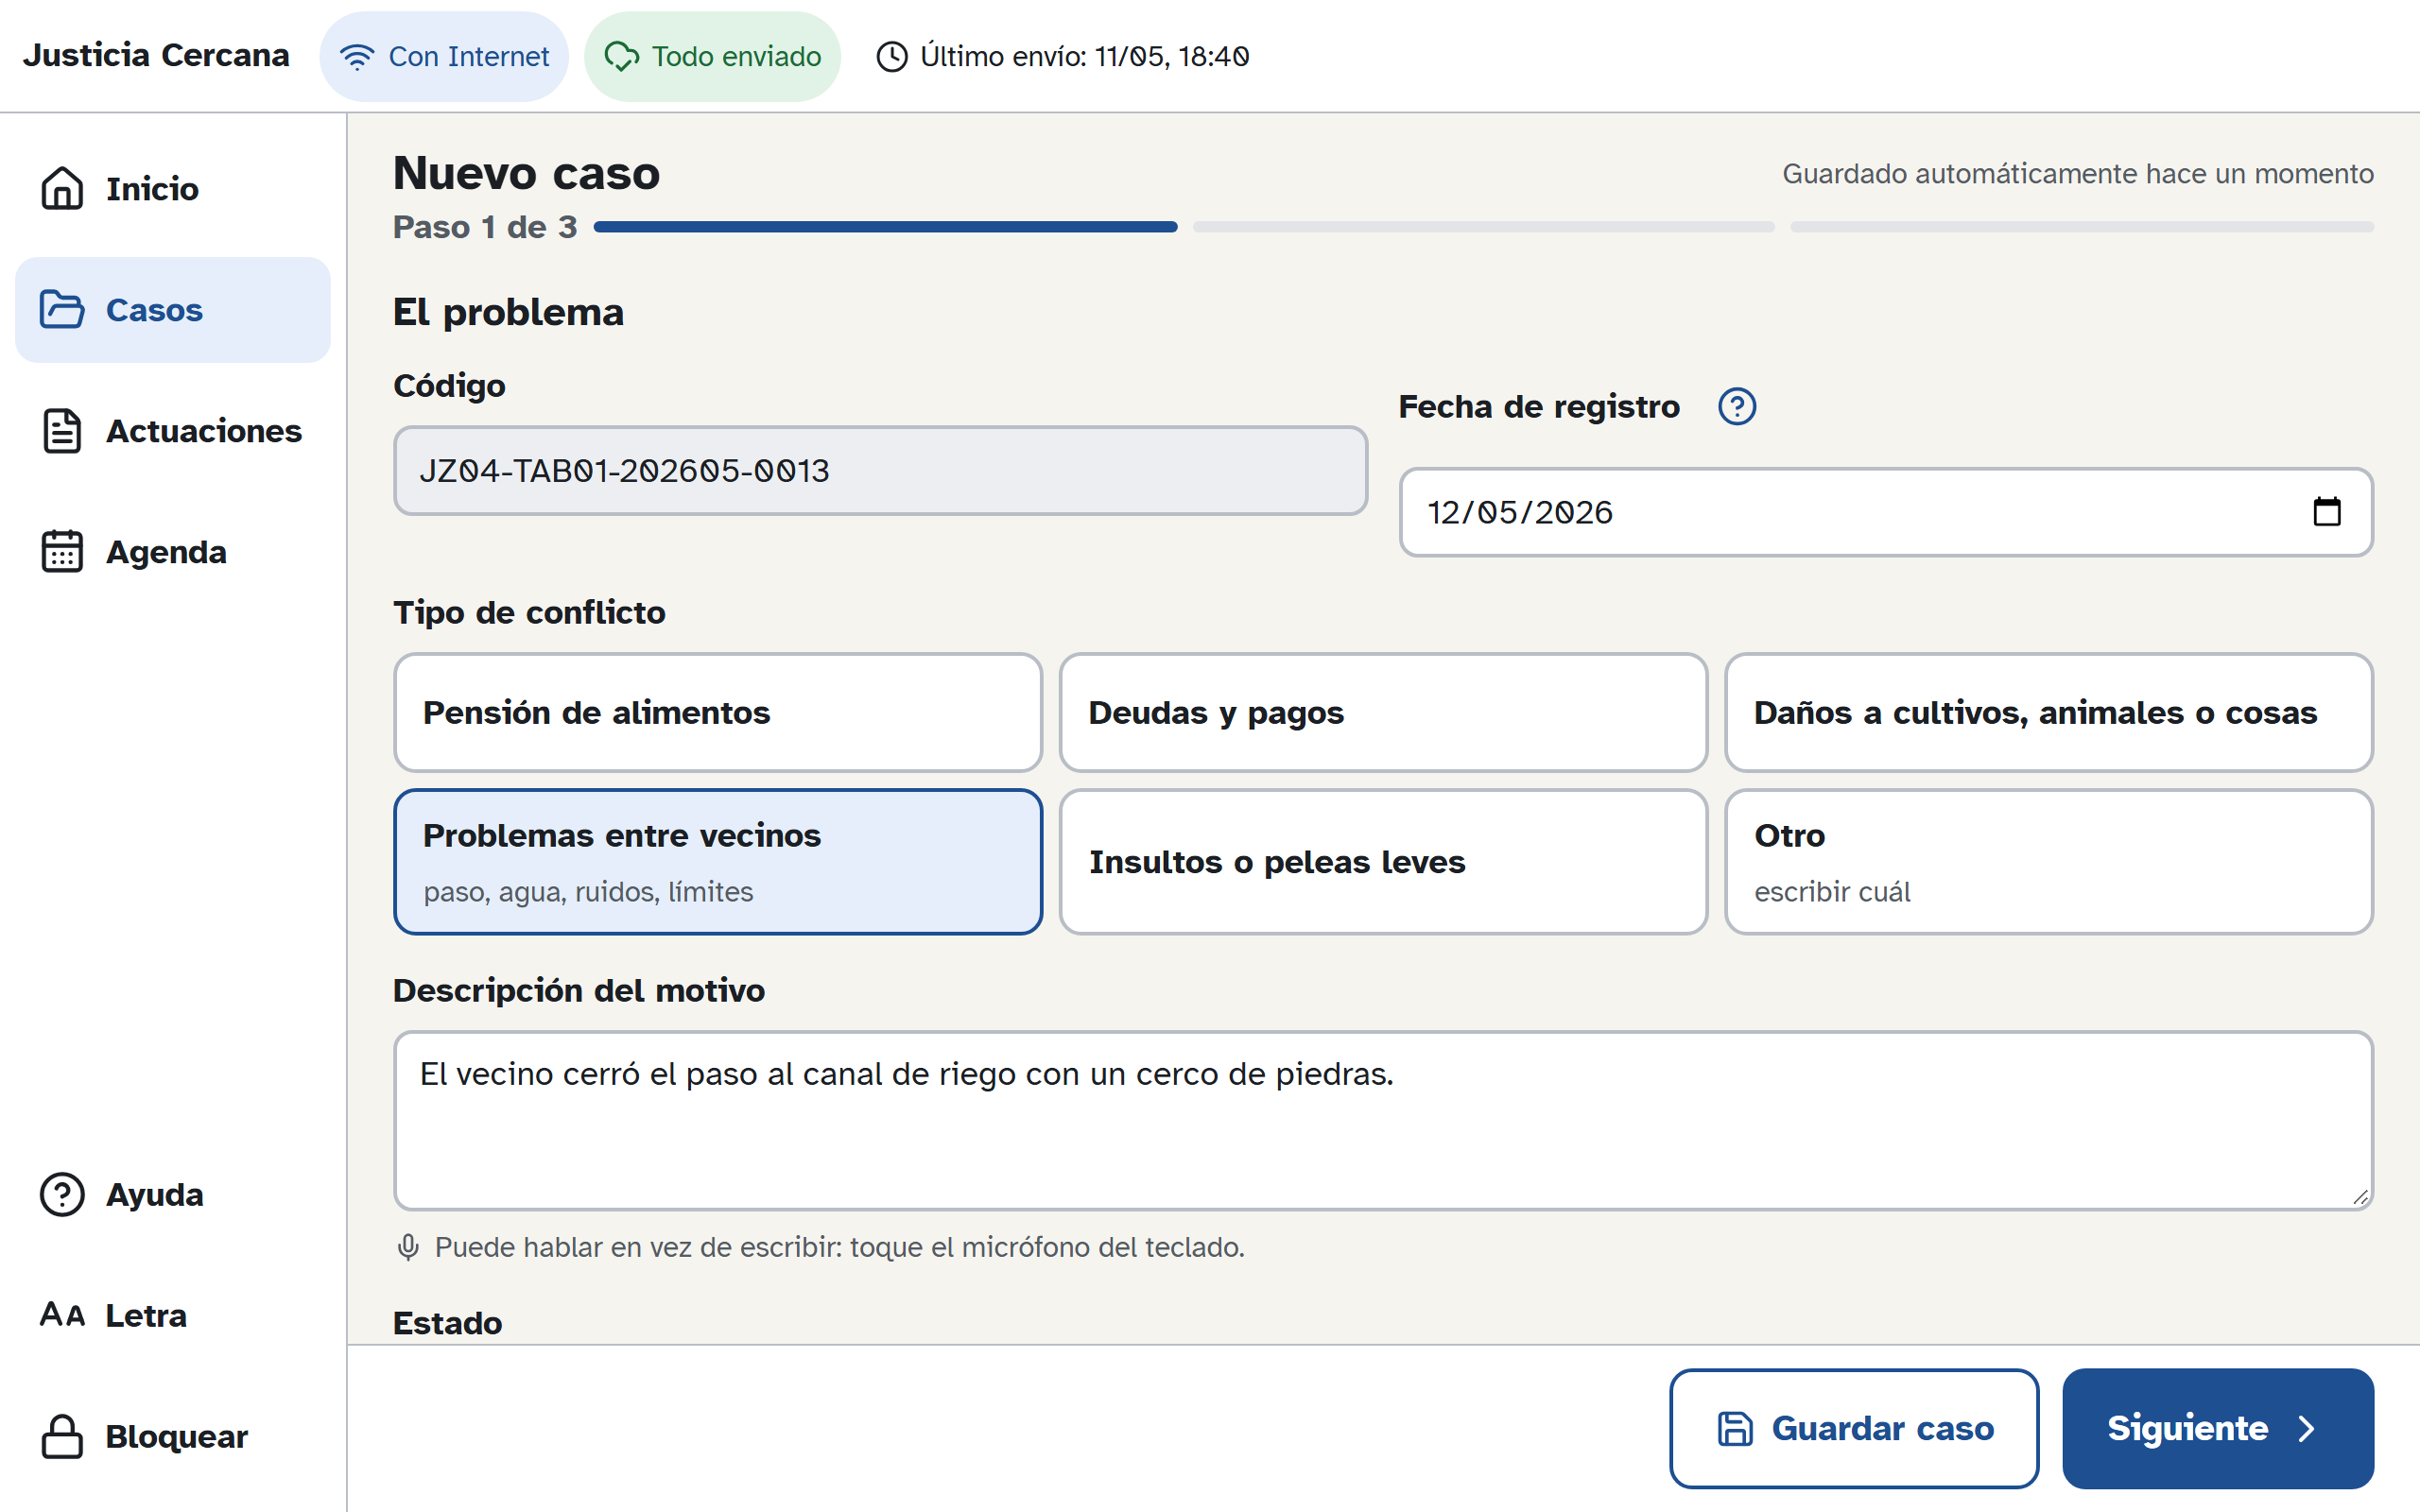
\includegraphics[width=\linewidth]{../../captures/F1-02_nuevo-caso-paso1.png}\\[-2pt]{\footnotesize\raggedright\textbf{P-03 · 2.} Paso 1 ``El problema'': tipo con botones grandes, descripción con ayuda de dictado y guardado automático \emph{(Cobertura y funcionamiento de los módulos)}\par}\end{minipage}\hfill
\begin{minipage}[t]{0.49\textwidth}\centering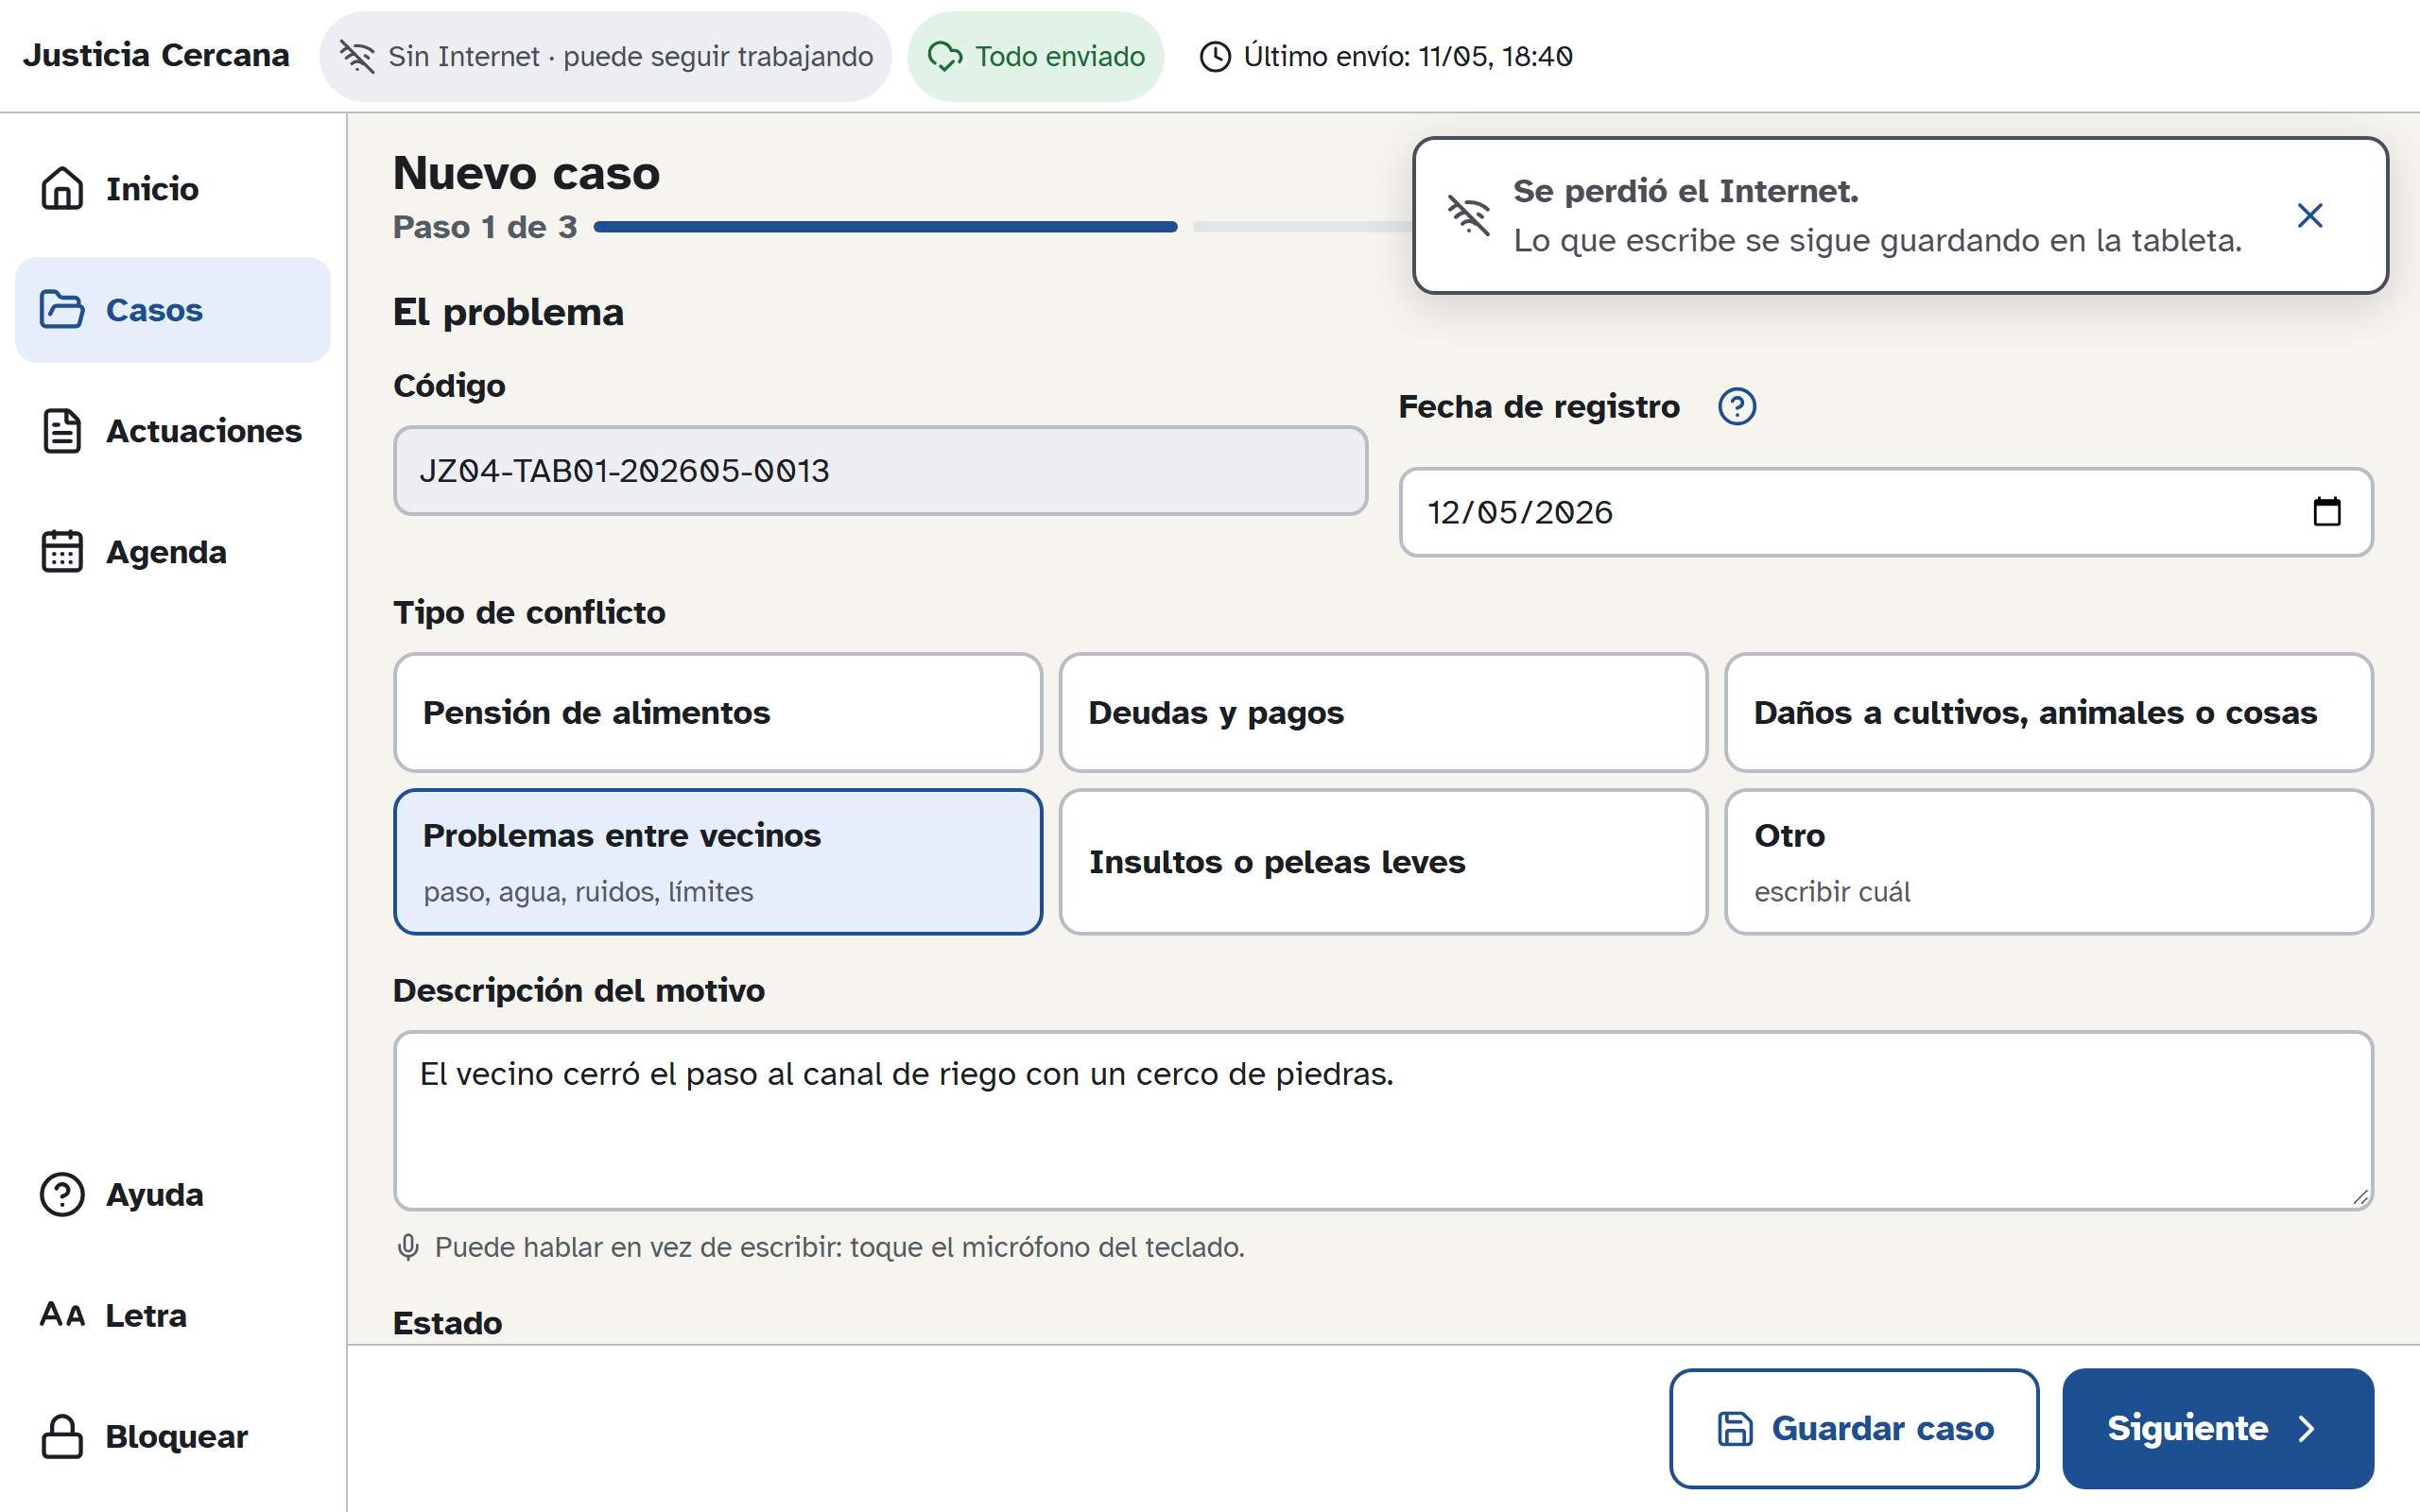
\includegraphics[width=\linewidth]{../../captures/F1-03_aviso-corte-internet.png}\\[-2pt]{\footnotesize\raggedright\textbf{P-03 · 3.} Corte real de Internet a mitad del formulario: aviso gris y barra ``Sin Internet'' \emph{(Funcionamiento sin conexión)}\par}\end{minipage}\par\vspace{8pt}\noindent
\begin{minipage}[t]{0.49\textwidth}\centering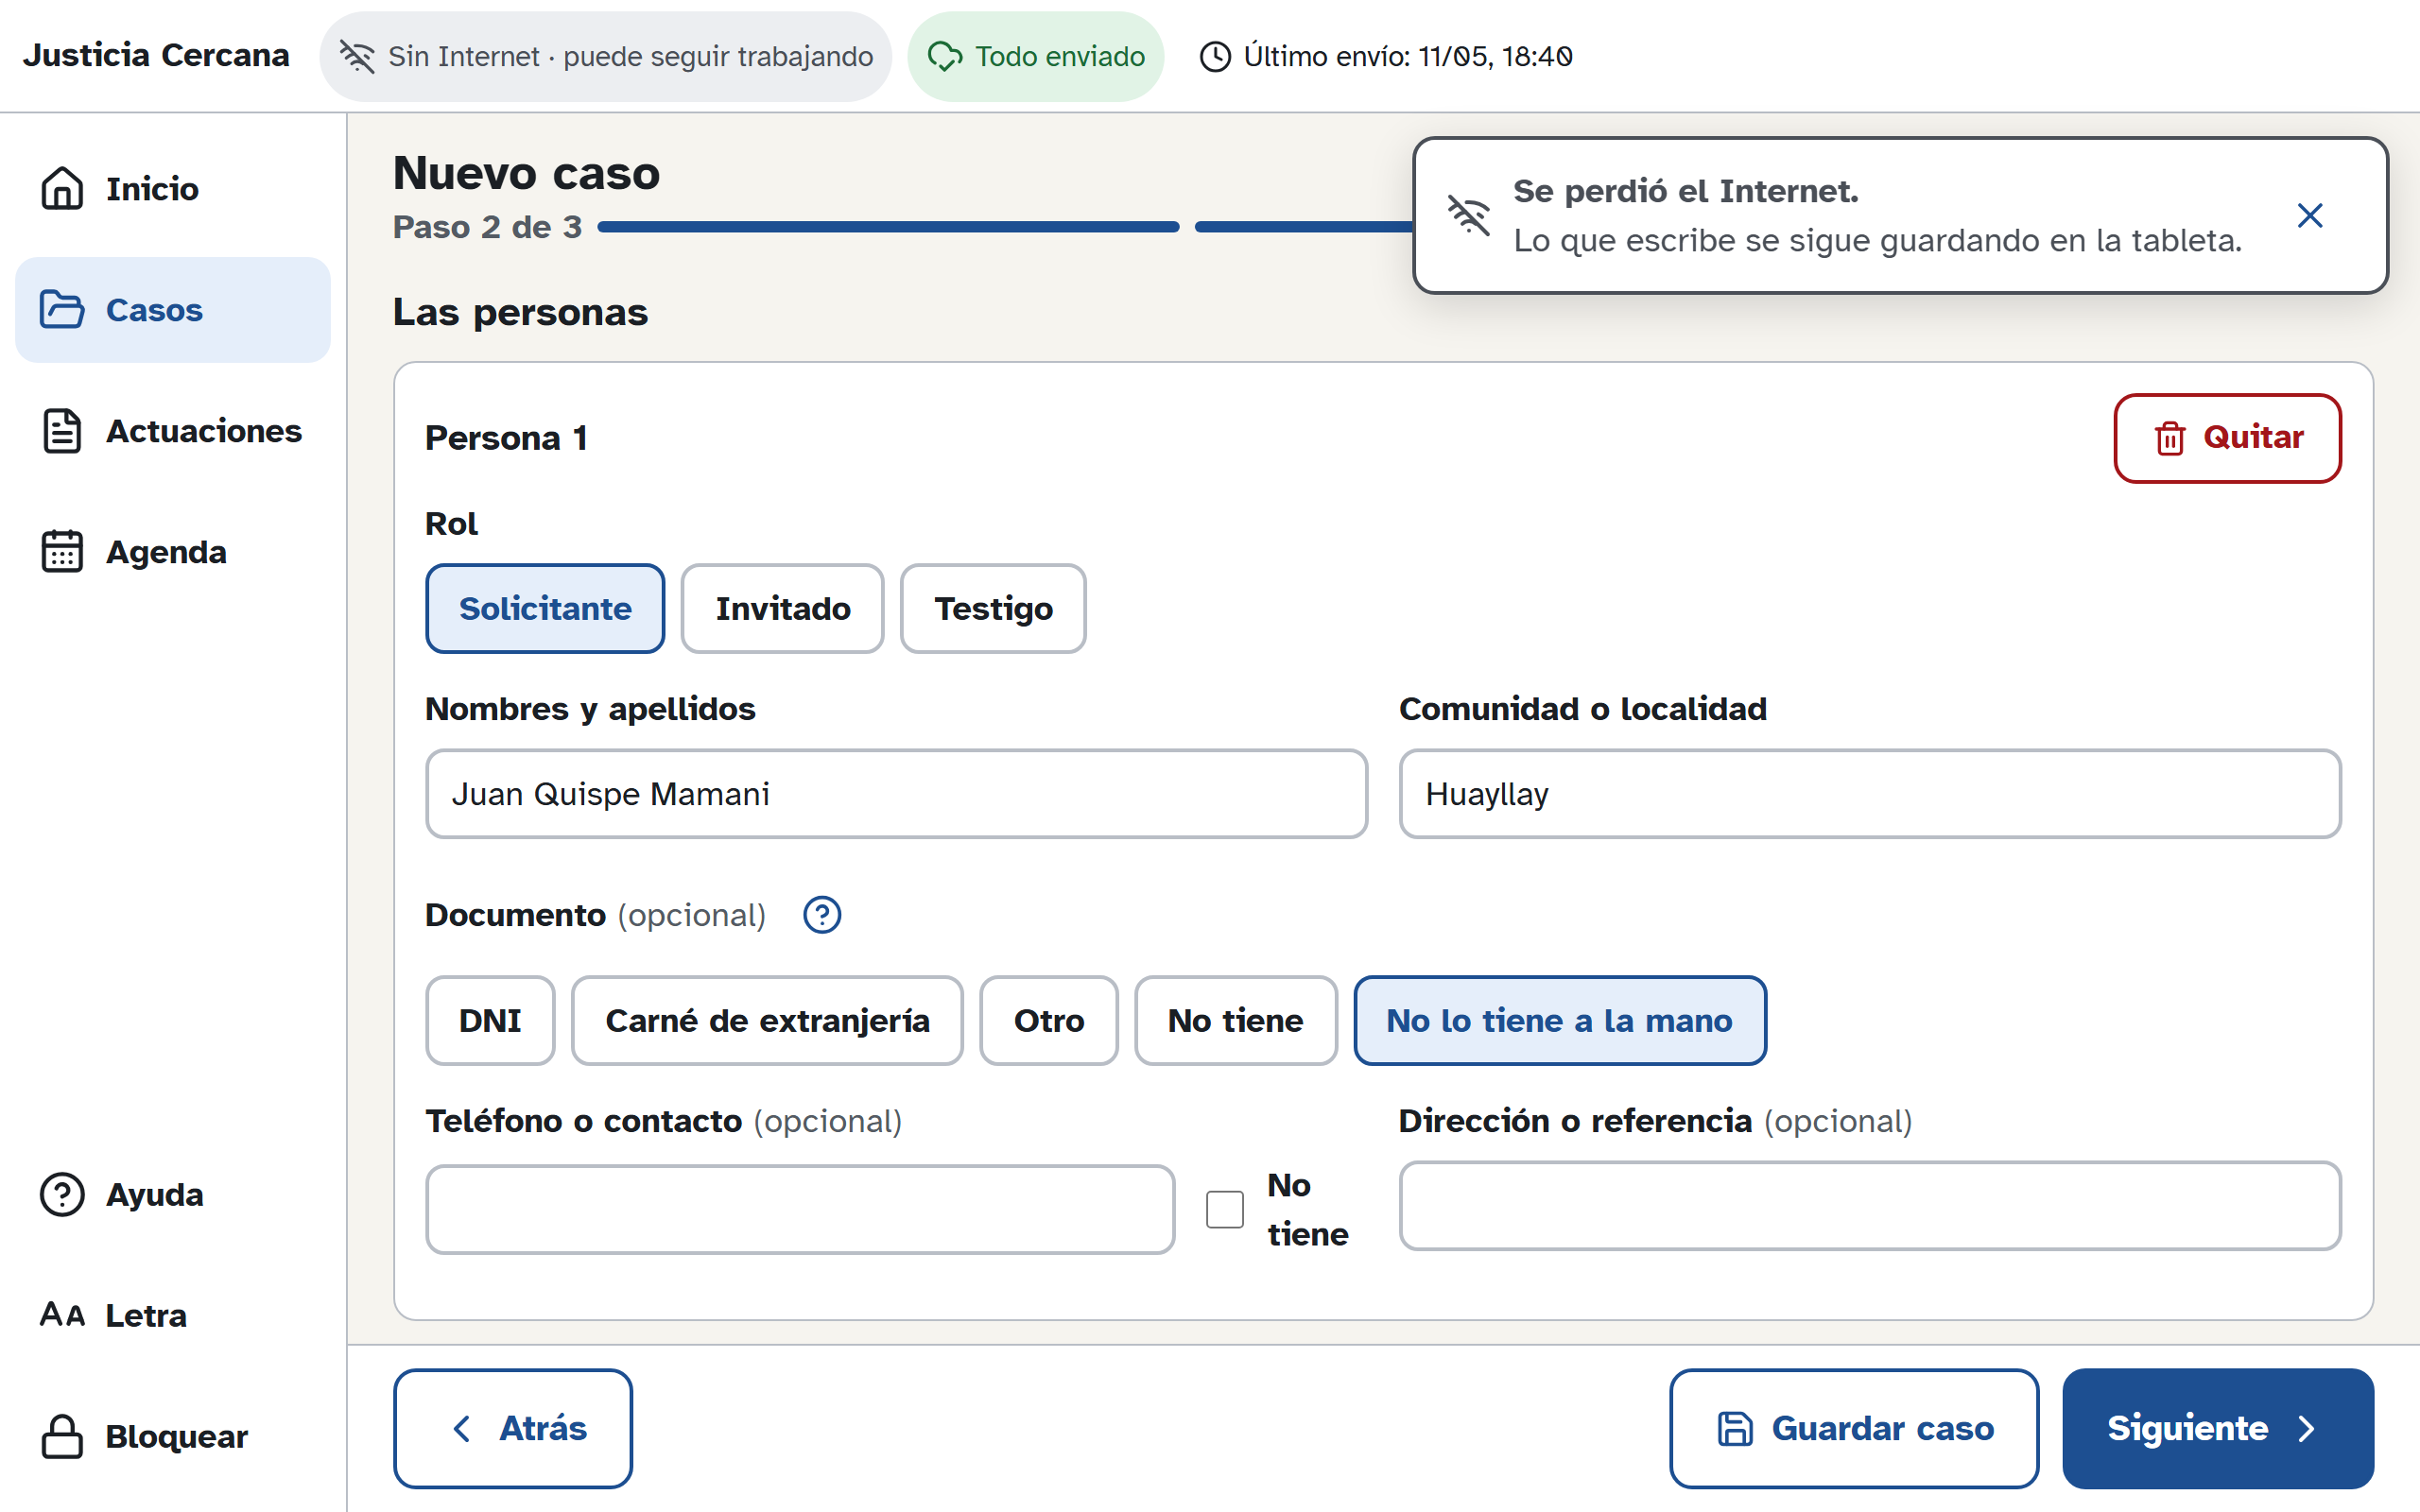
\includegraphics[width=\linewidth]{../../captures/F1-04_parte1-solicitante.png}\\[-2pt]{\footnotesize\raggedright\textbf{P-03 · 4.} Parte 1 con rol, patrón ``No lo tiene a la mano'' y comunidad, sin Internet \emph{(Cobertura y funcionamiento de los módulos)}\par}\end{minipage}\hfill
\begin{minipage}[t]{0.49\textwidth}\centering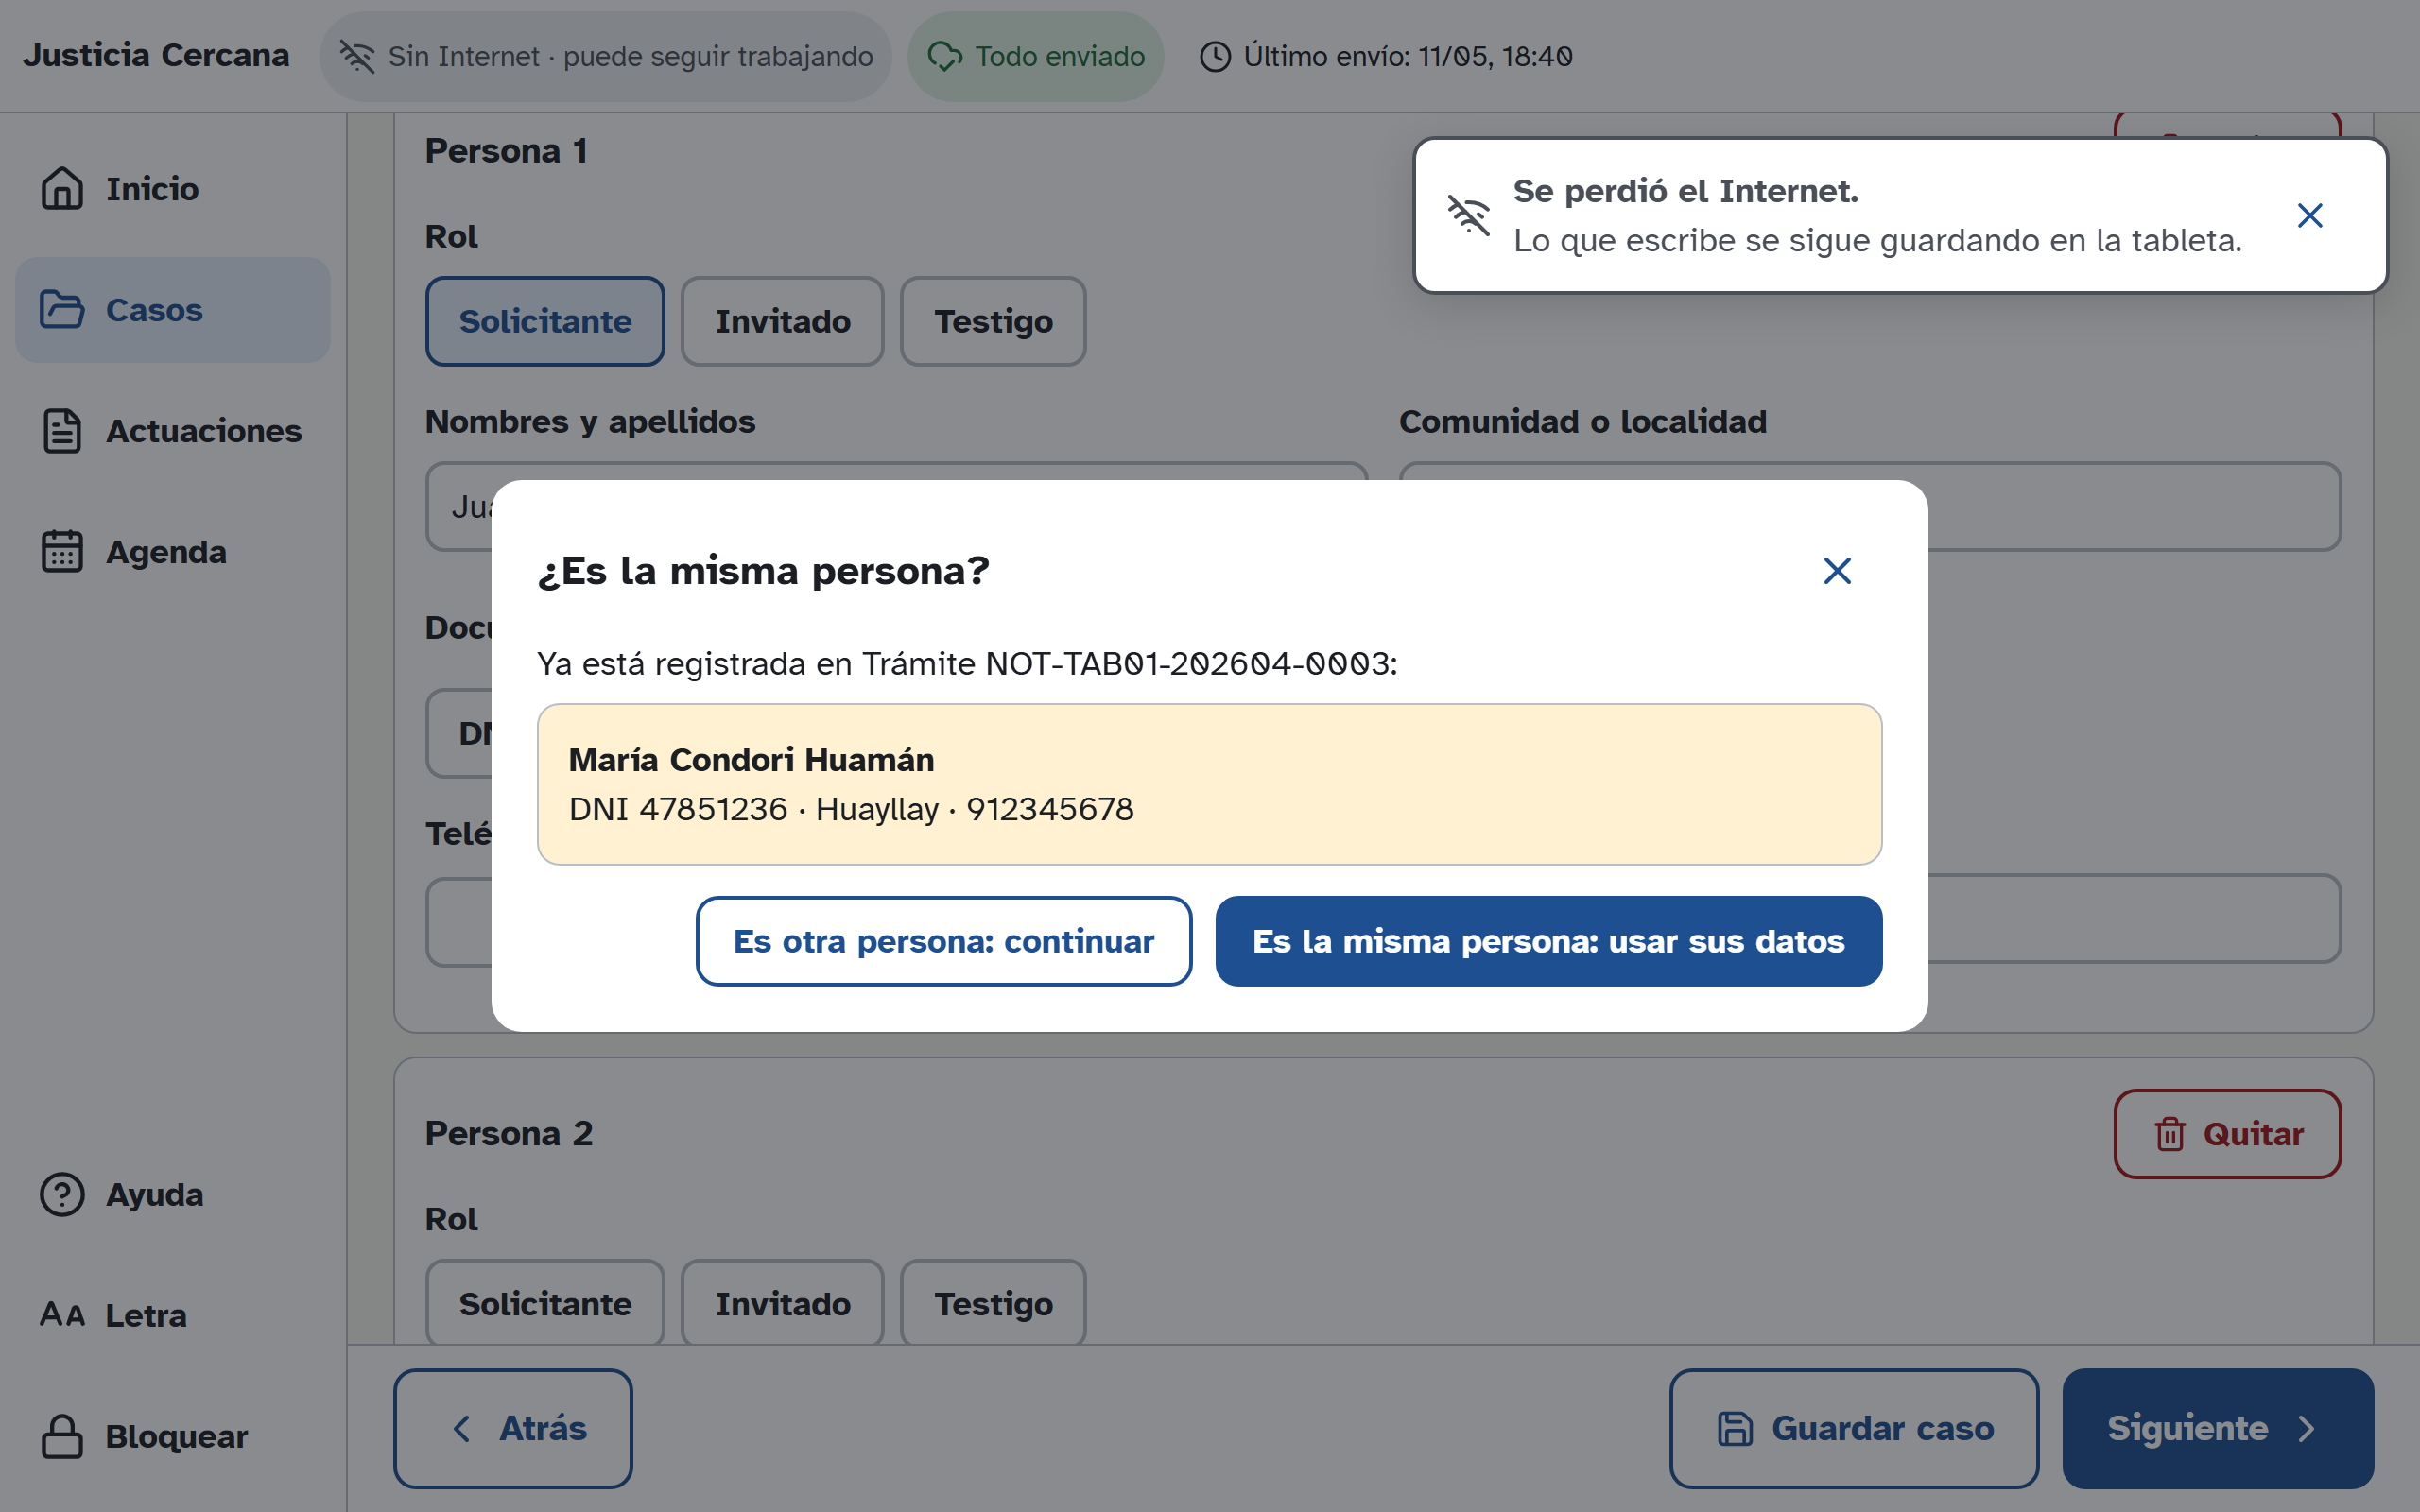
\includegraphics[width=\linewidth]{../../captures/F1-05a_advertencia-duplicado.png}\\[-2pt]{\footnotesize\raggedright\textbf{P-03 · 5.} Advertencia de duplicado (regla 5.3) que no bloquea \emph{(Principios de diseño y heurísticas)}\par}\end{minipage}\par\vspace{8pt}\noindent
\begin{minipage}[t]{0.49\textwidth}\centering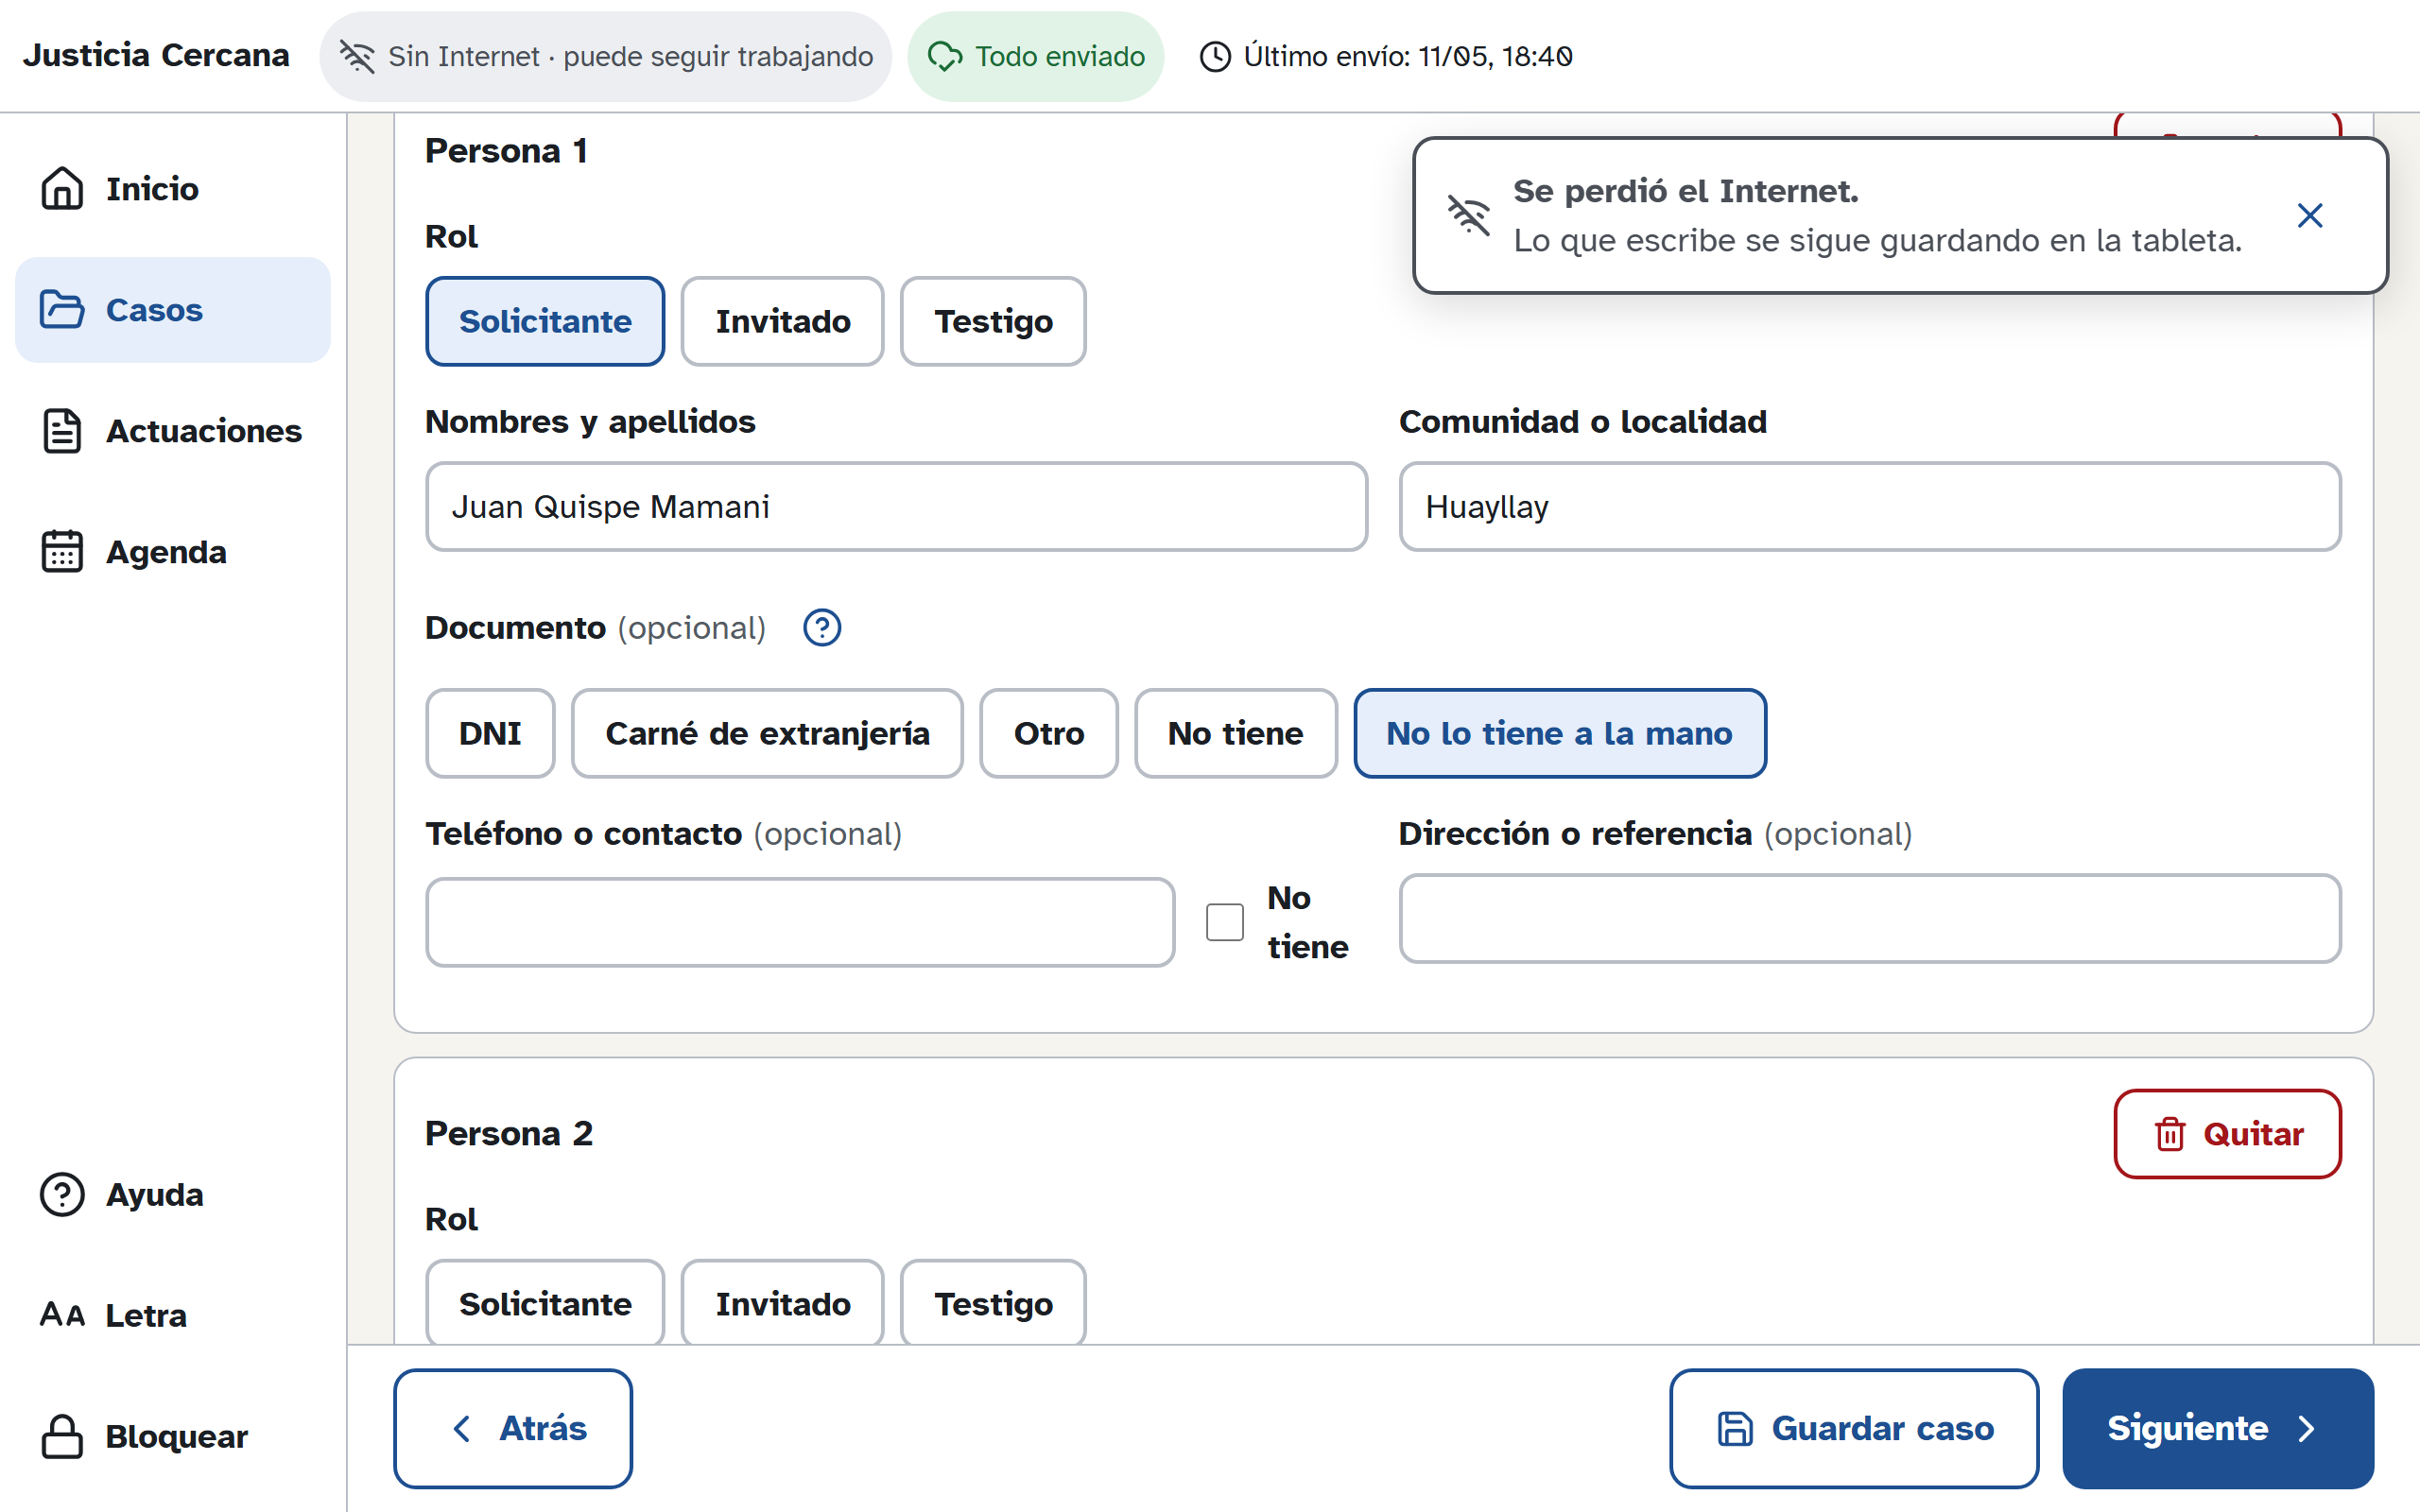
\includegraphics[width=\linewidth]{../../captures/F1-05b_datos-reutilizados.png}\\[-2pt]{\footnotesize\raggedright\textbf{P-03 · 5.} Se reutilizan los datos de la persona ya registrada \emph{(Principios de diseño y heurísticas)}\par}\end{minipage}\hfill
\begin{minipage}[t]{0.49\textwidth}\centering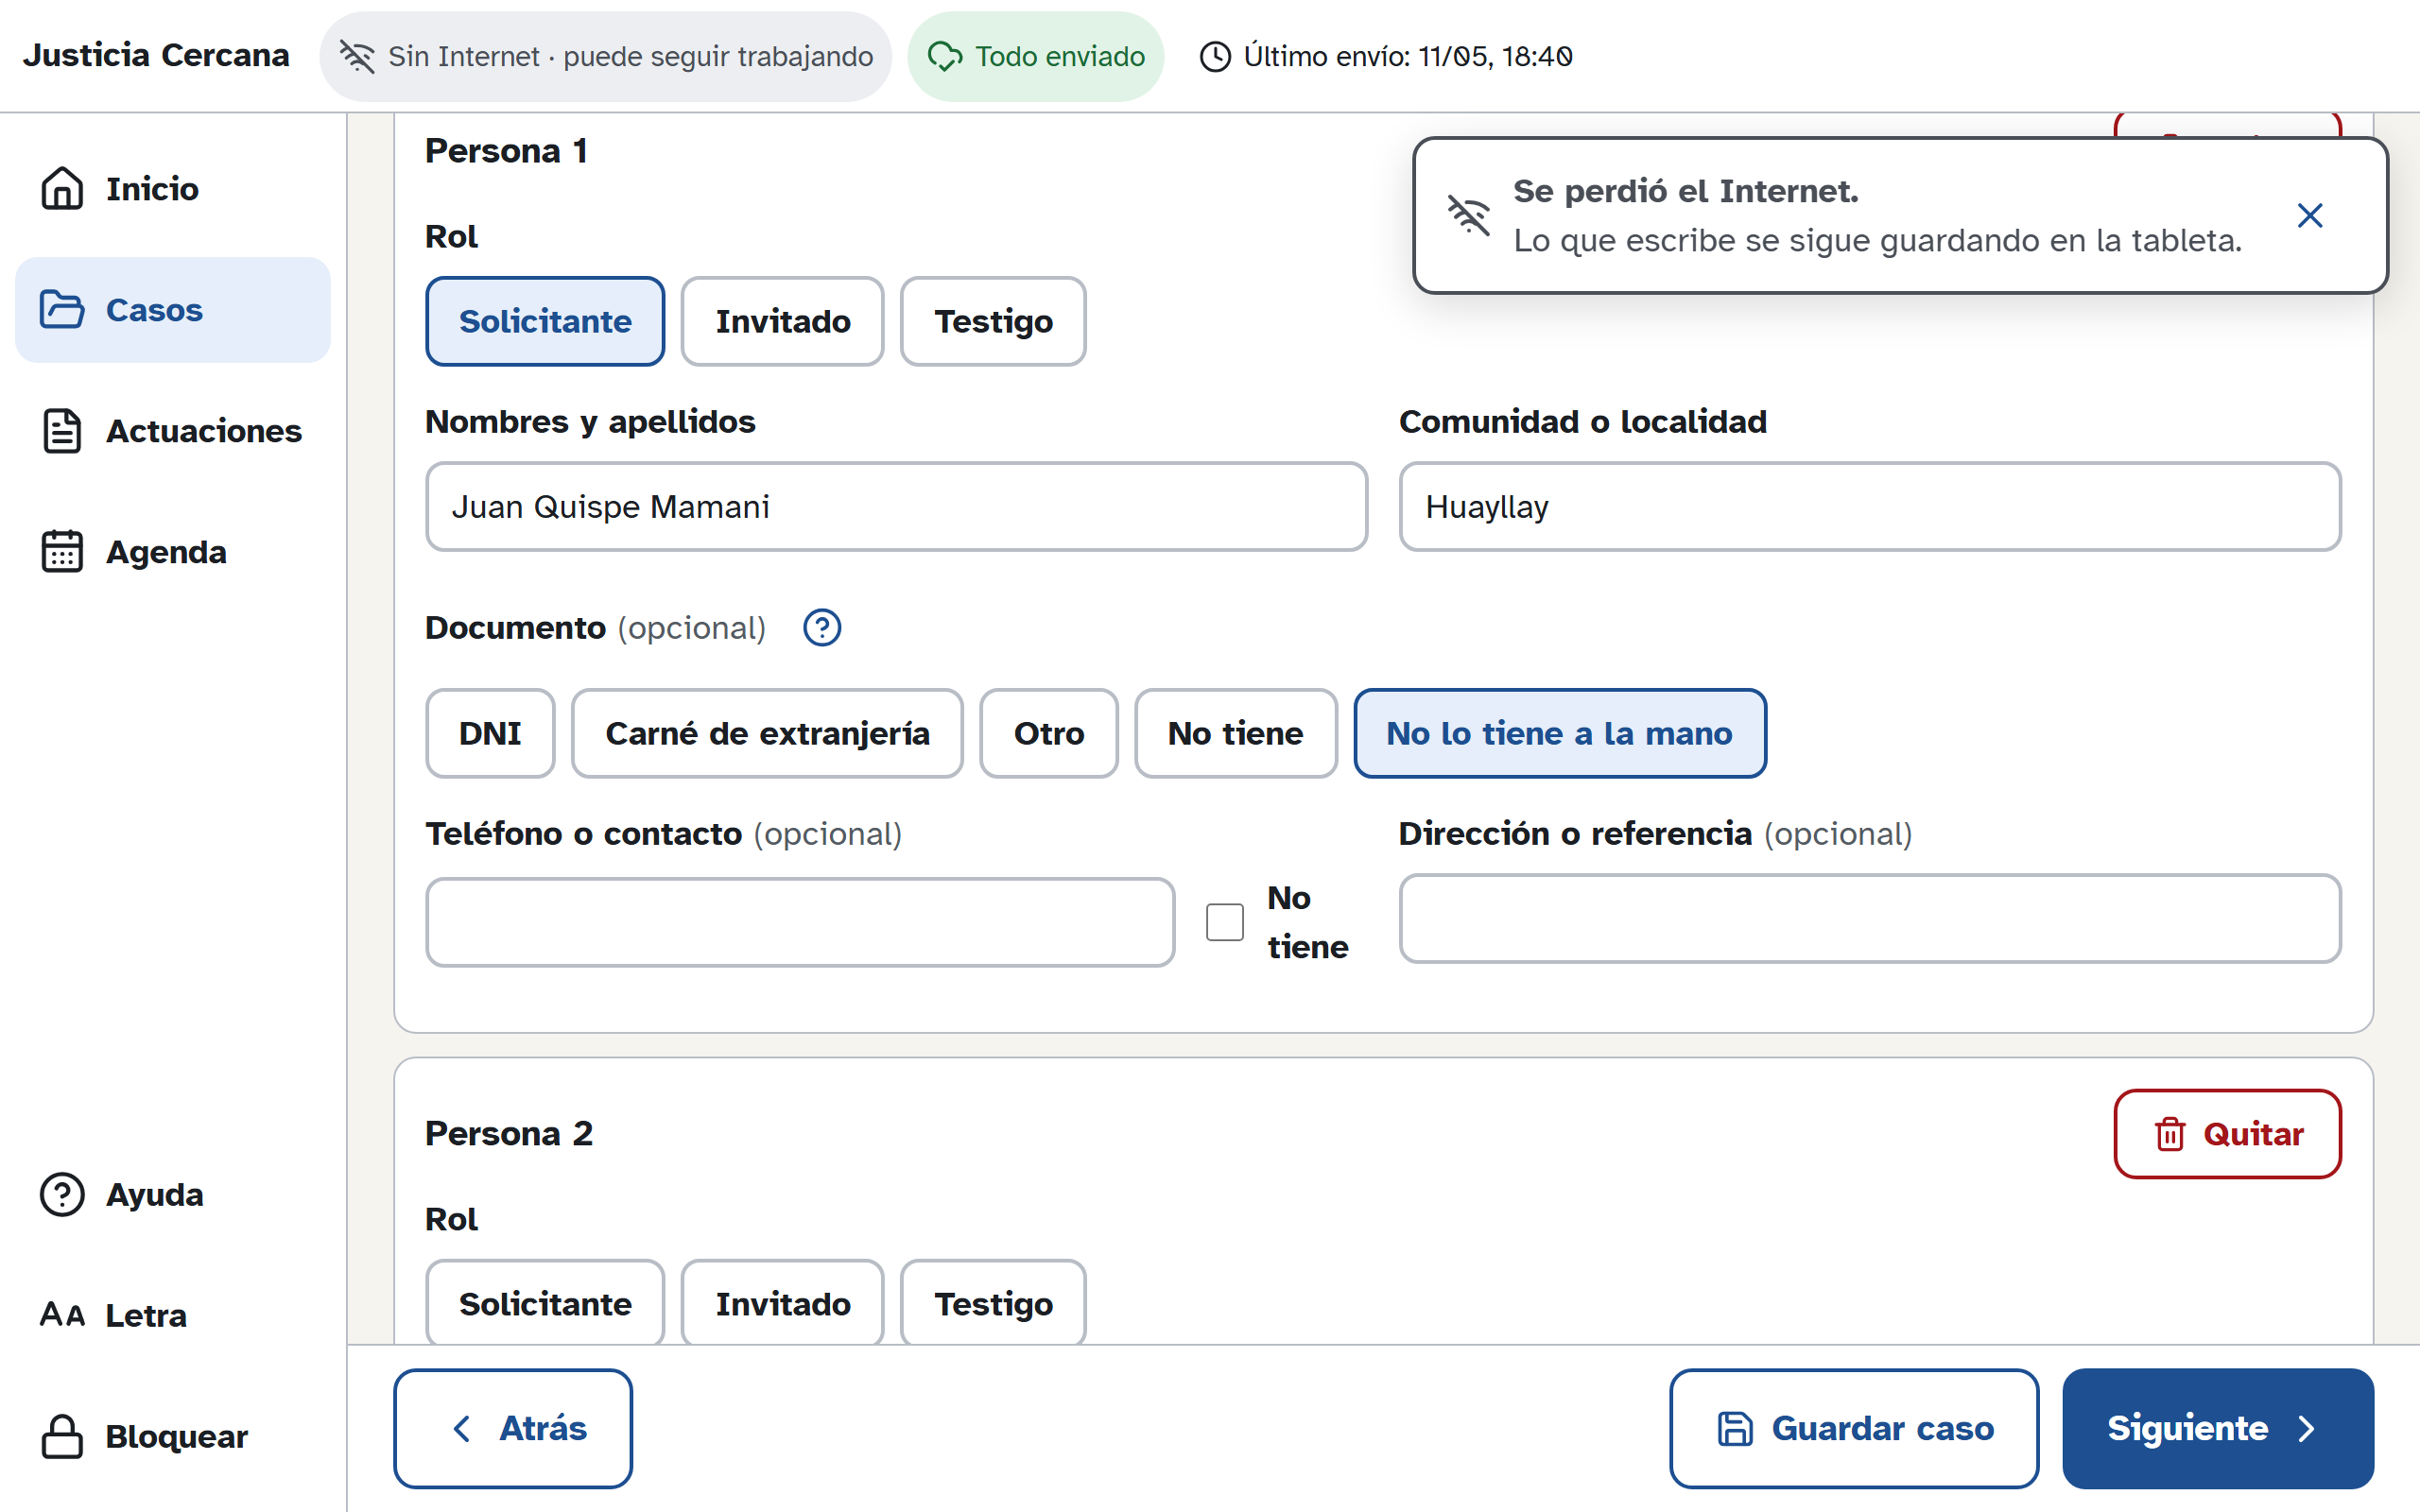
\includegraphics[width=\linewidth]{../../captures/F1-06_error-sin-rol.png}\\[-2pt]{\footnotesize\raggedright\textbf{P-03 · 6.} Error de validación en lenguaje simple junto al campo \emph{(Principios de diseño y heurísticas)}\par}\end{minipage}\par\vspace{8pt}\noindent
\begin{minipage}[t]{0.49\textwidth}\centering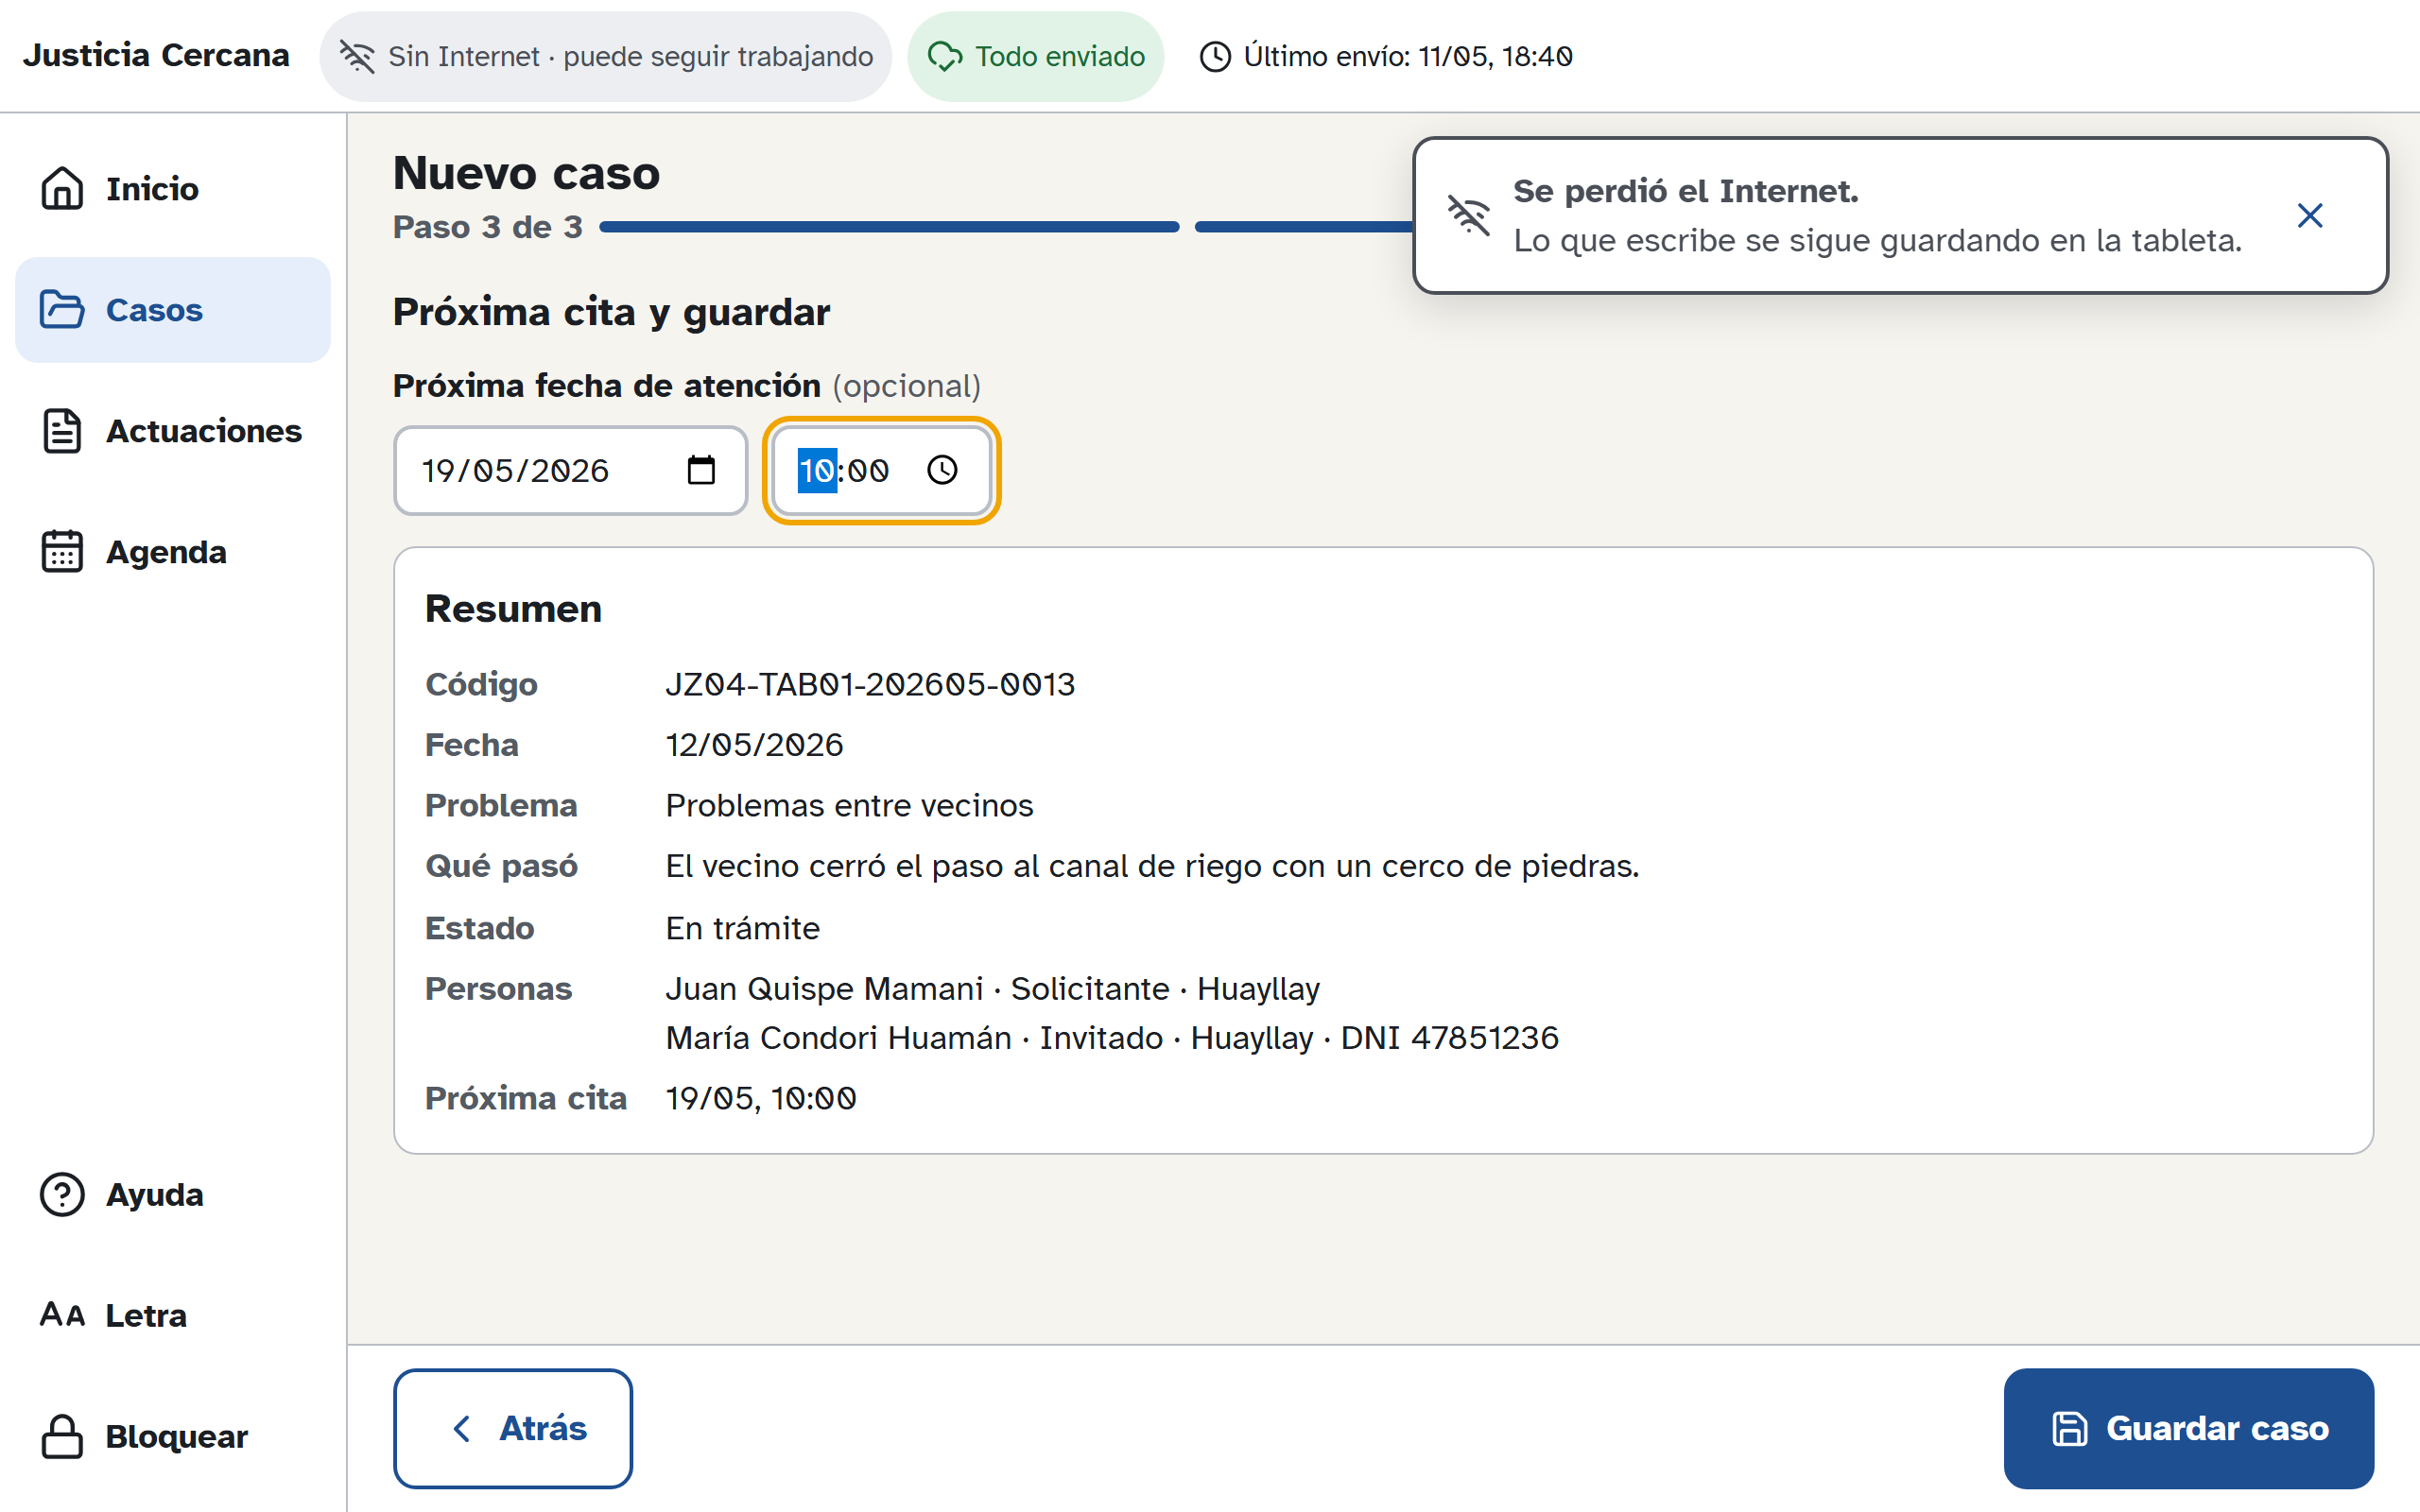
\includegraphics[width=\linewidth]{../../captures/F1-07_resumen-proxima-cita.png}\\[-2pt]{\footnotesize\raggedright\textbf{P-03 · 7.} Próxima cita 19/05 10:00 y resumen legible antes de guardar \emph{(Cobertura y funcionamiento de los módulos)}\par}\end{minipage}\hfill
\begin{minipage}[t]{0.49\textwidth}\centering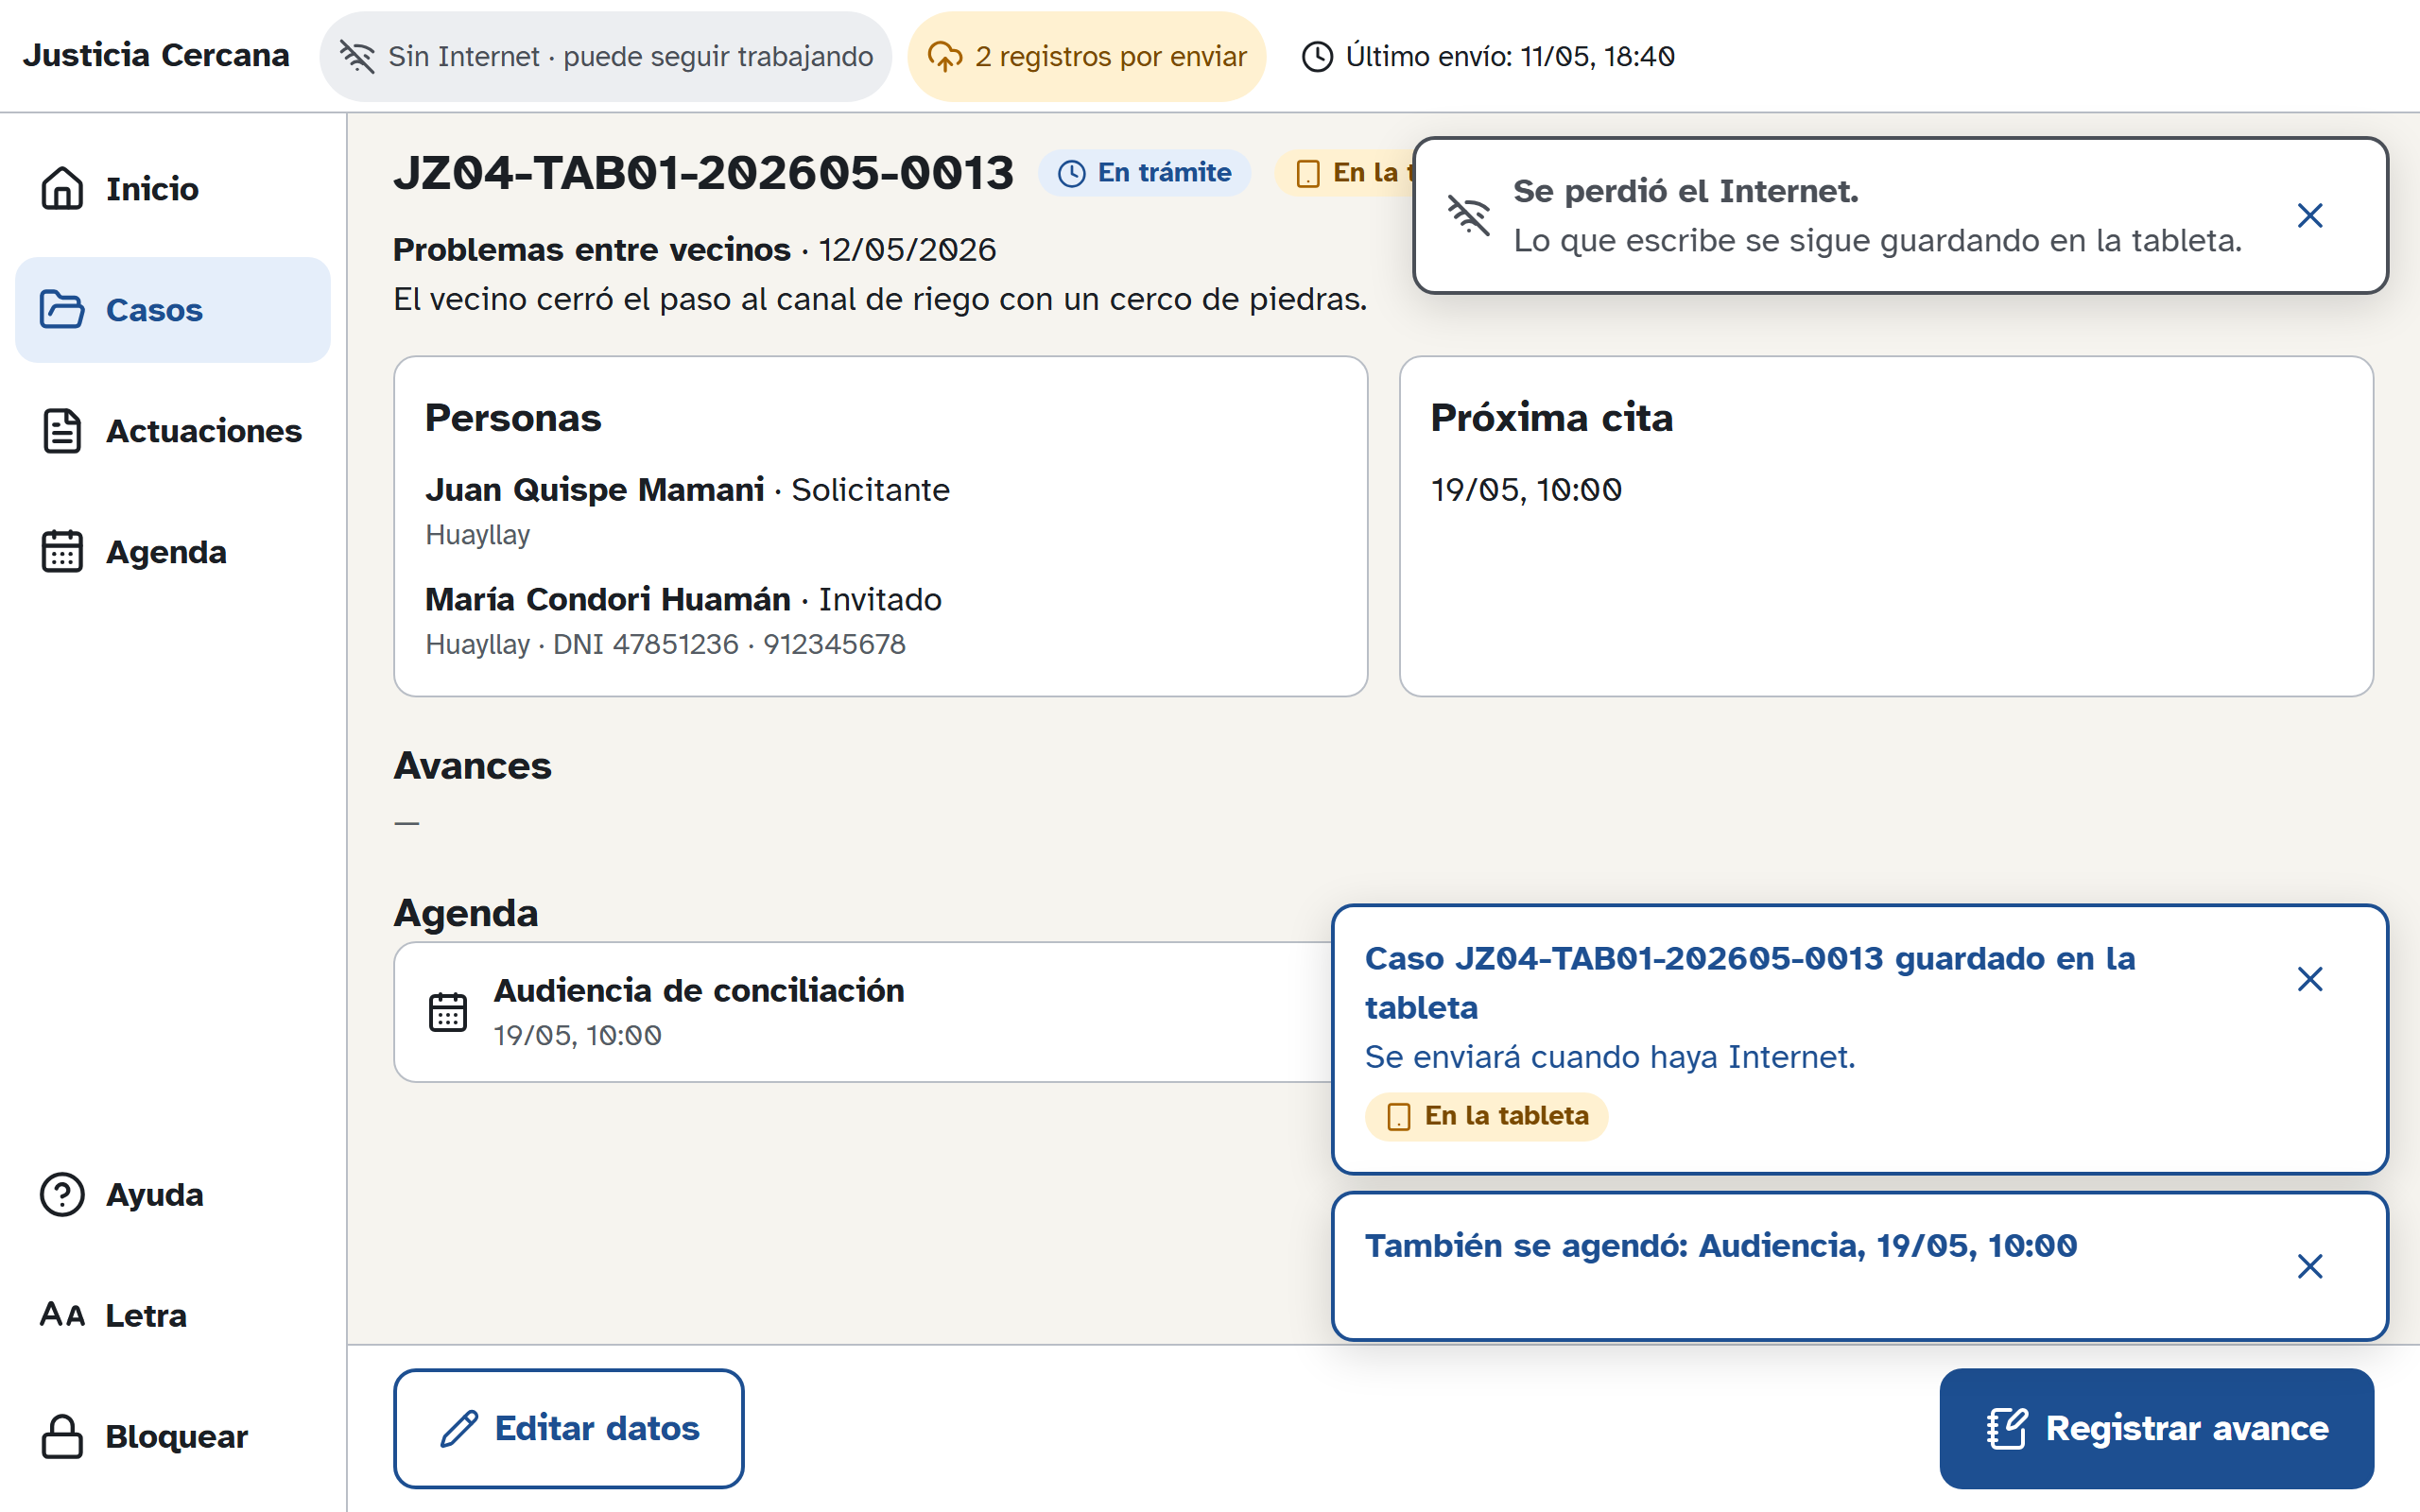
\includegraphics[width=\linewidth]{../../captures/F1-08_confirmacion-guardado.png}\\[-2pt]{\footnotesize\raggedright\textbf{P-04 · 8.} Confirmación ``guardado en la tableta'' + ``También se agendó'' y barra ``2 registros por enviar'' \emph{(Funcionamiento sin conexión)}\par}\end{minipage}\par\vspace{8pt}\noindent
\par\vspace{4pt}
\subsection*{Flujo 2}
\noindent
\begin{minipage}[t]{0.49\textwidth}\centering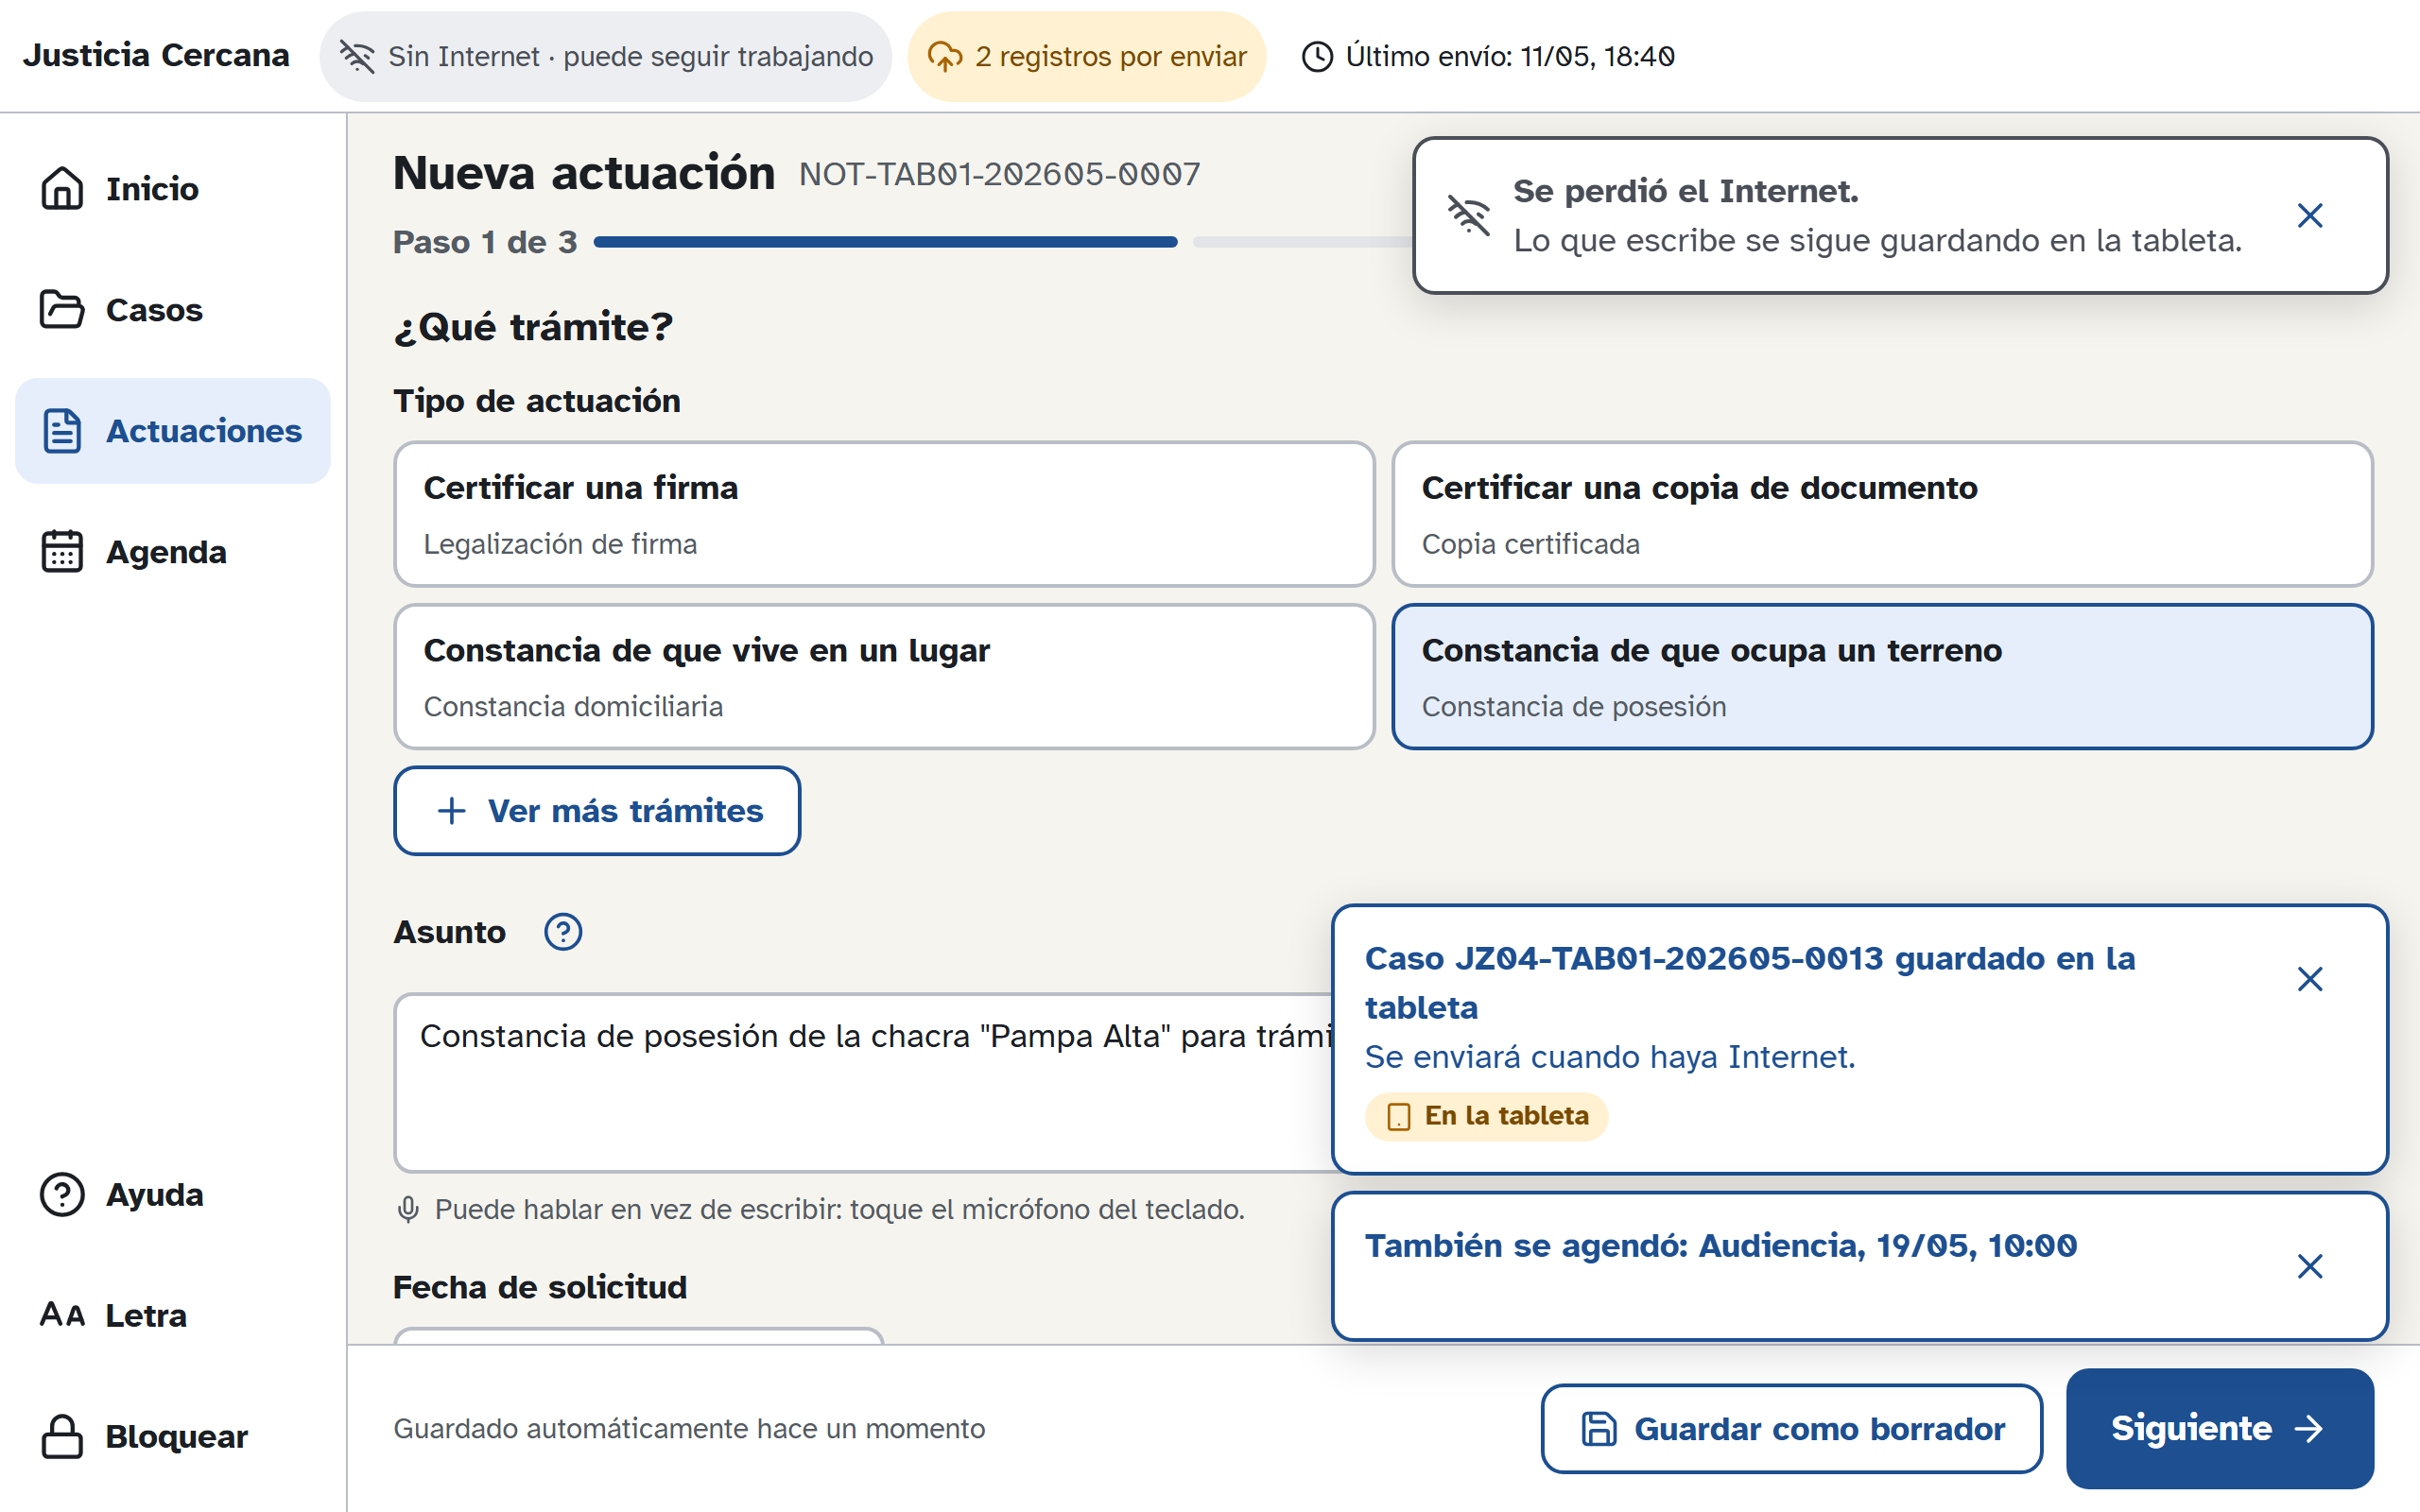
\includegraphics[width=\linewidth]{../../captures/F2-01_tipo-y-asunto.png}\\[-2pt]{\footnotesize\raggedright\textbf{P-06 · 1.} Tipo en lenguaje cotidiano (4 tarjetas + Ver más) y asunto \emph{(Cobertura y funcionamiento de los módulos)}\par}\end{minipage}\hfill
\begin{minipage}[t]{0.49\textwidth}\centering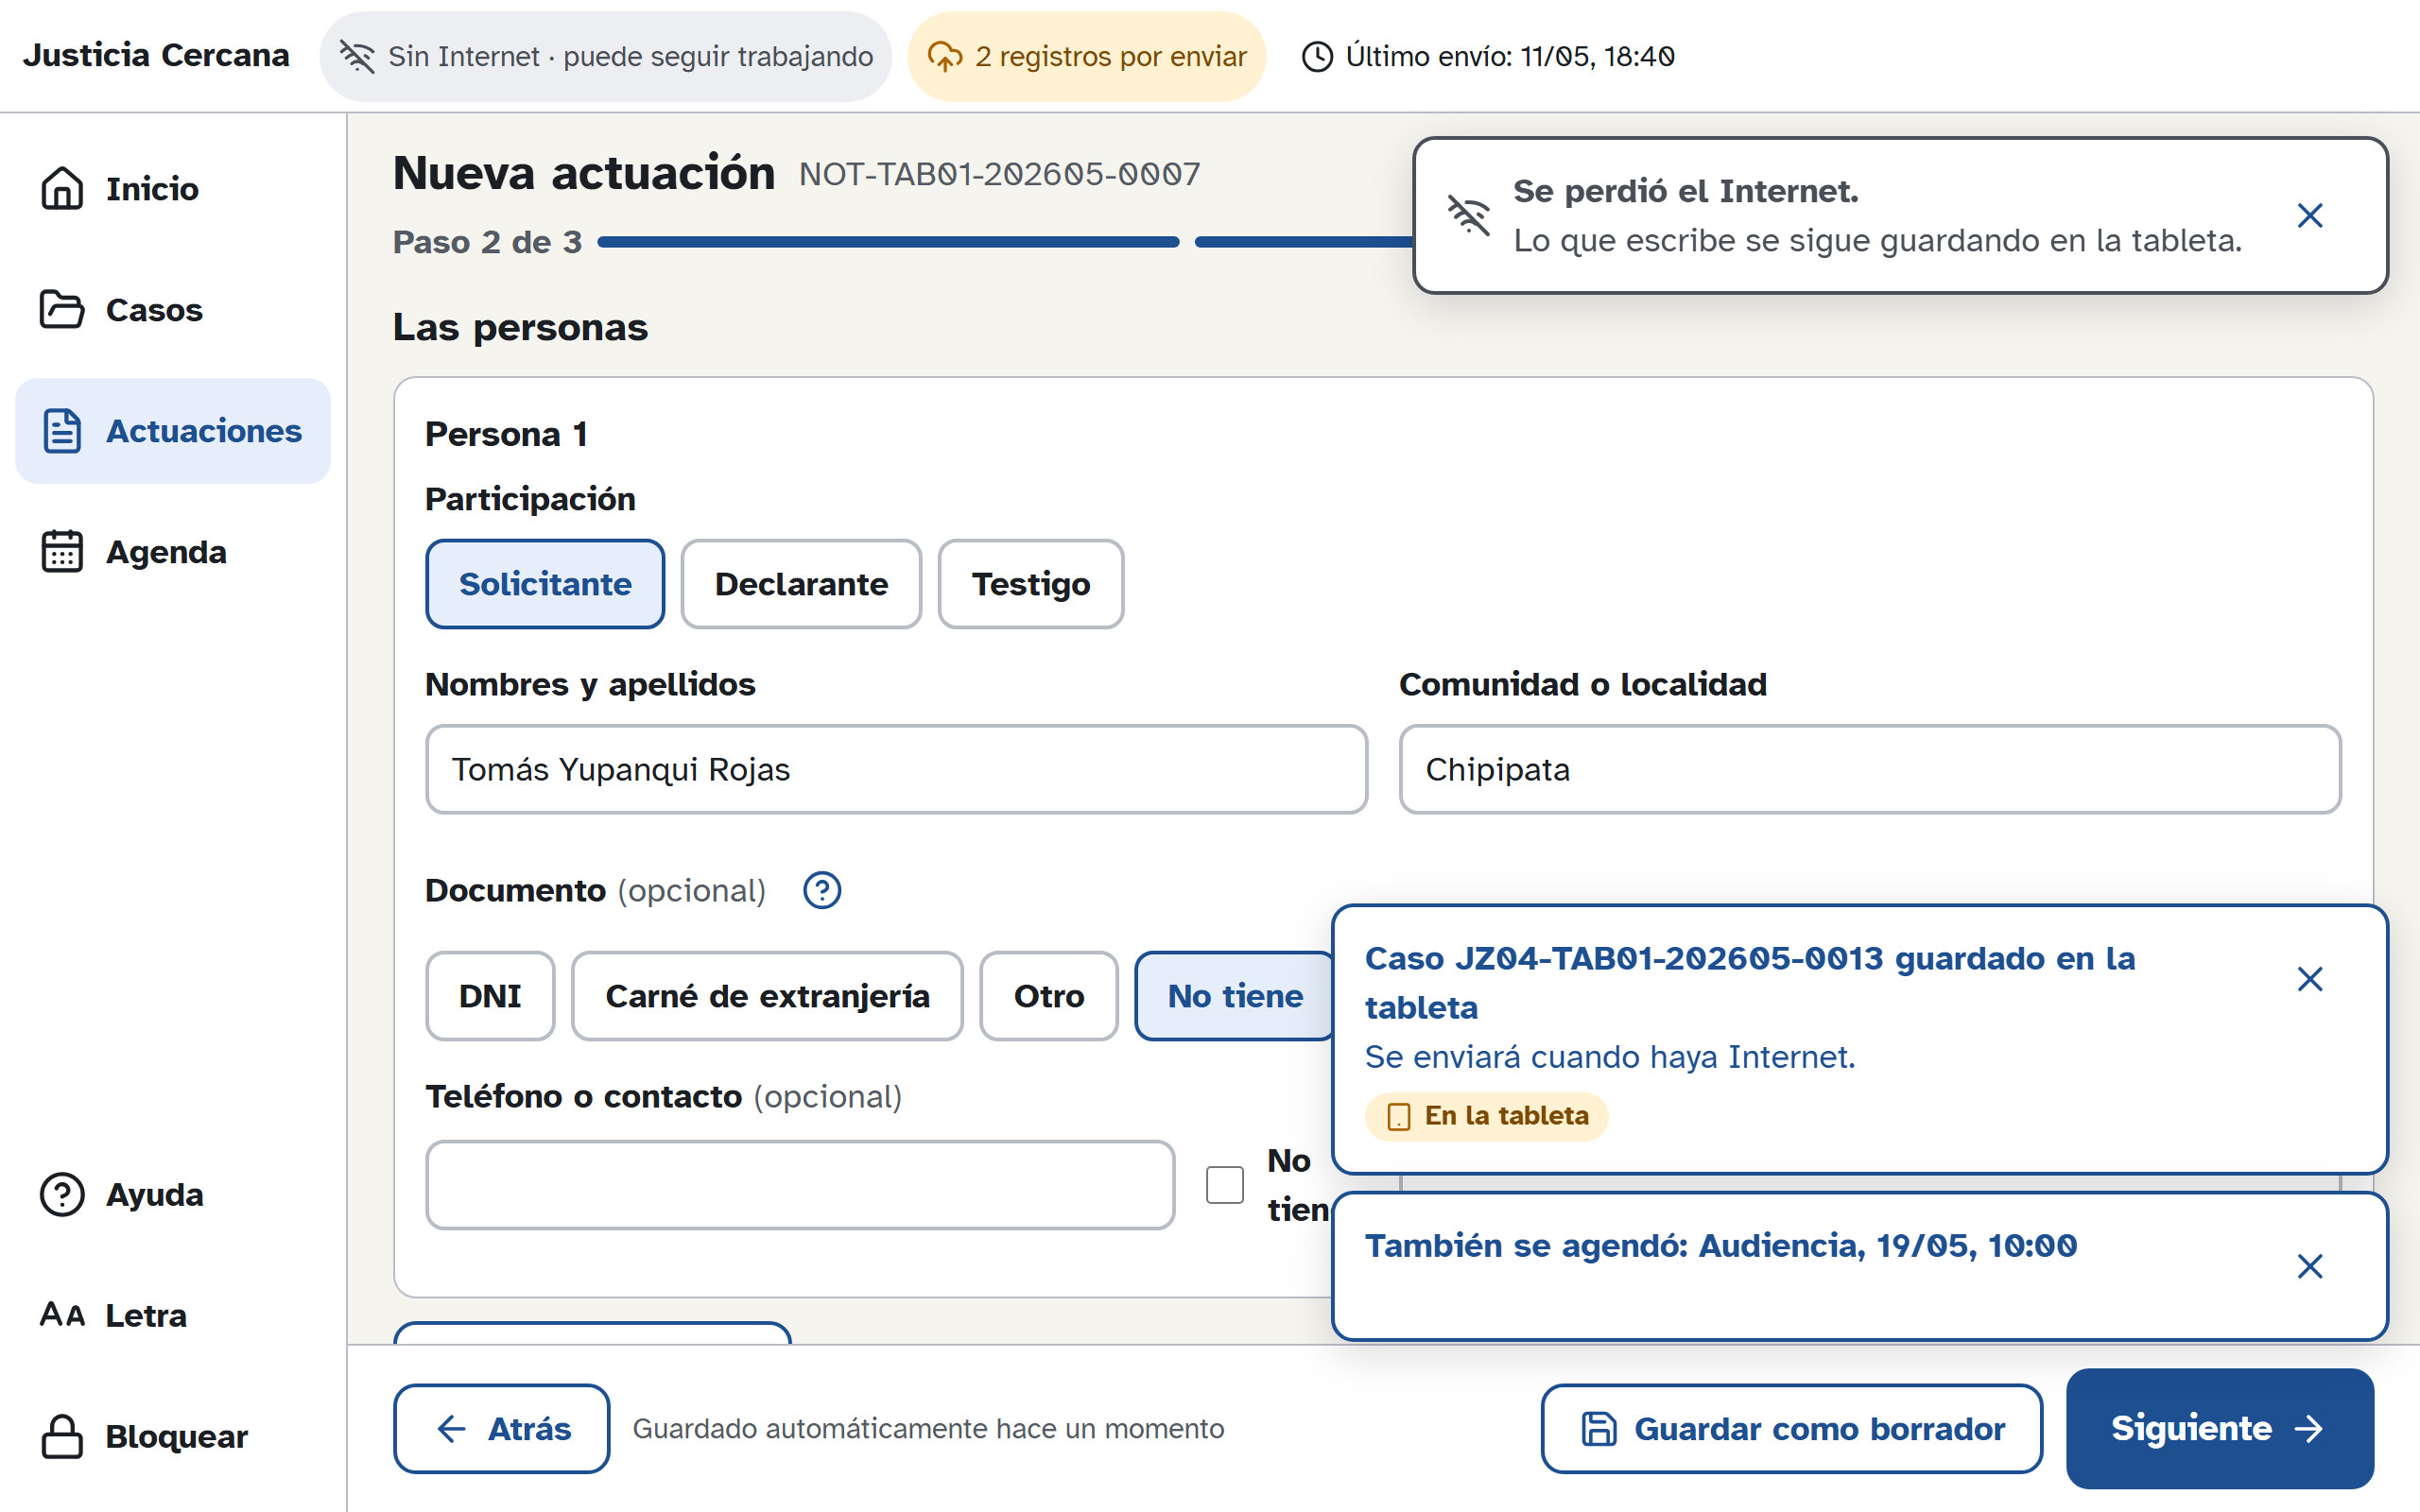
\includegraphics[width=\linewidth]{../../captures/F2-02_solicitante.png}\\[-2pt]{\footnotesize\raggedright\textbf{P-06 · 2.} Solicitante agregado sin duplicados; guardado automático \emph{(Cobertura y funcionamiento de los módulos)}\par}\end{minipage}\par\vspace{8pt}\noindent
\begin{minipage}[t]{0.49\textwidth}\centering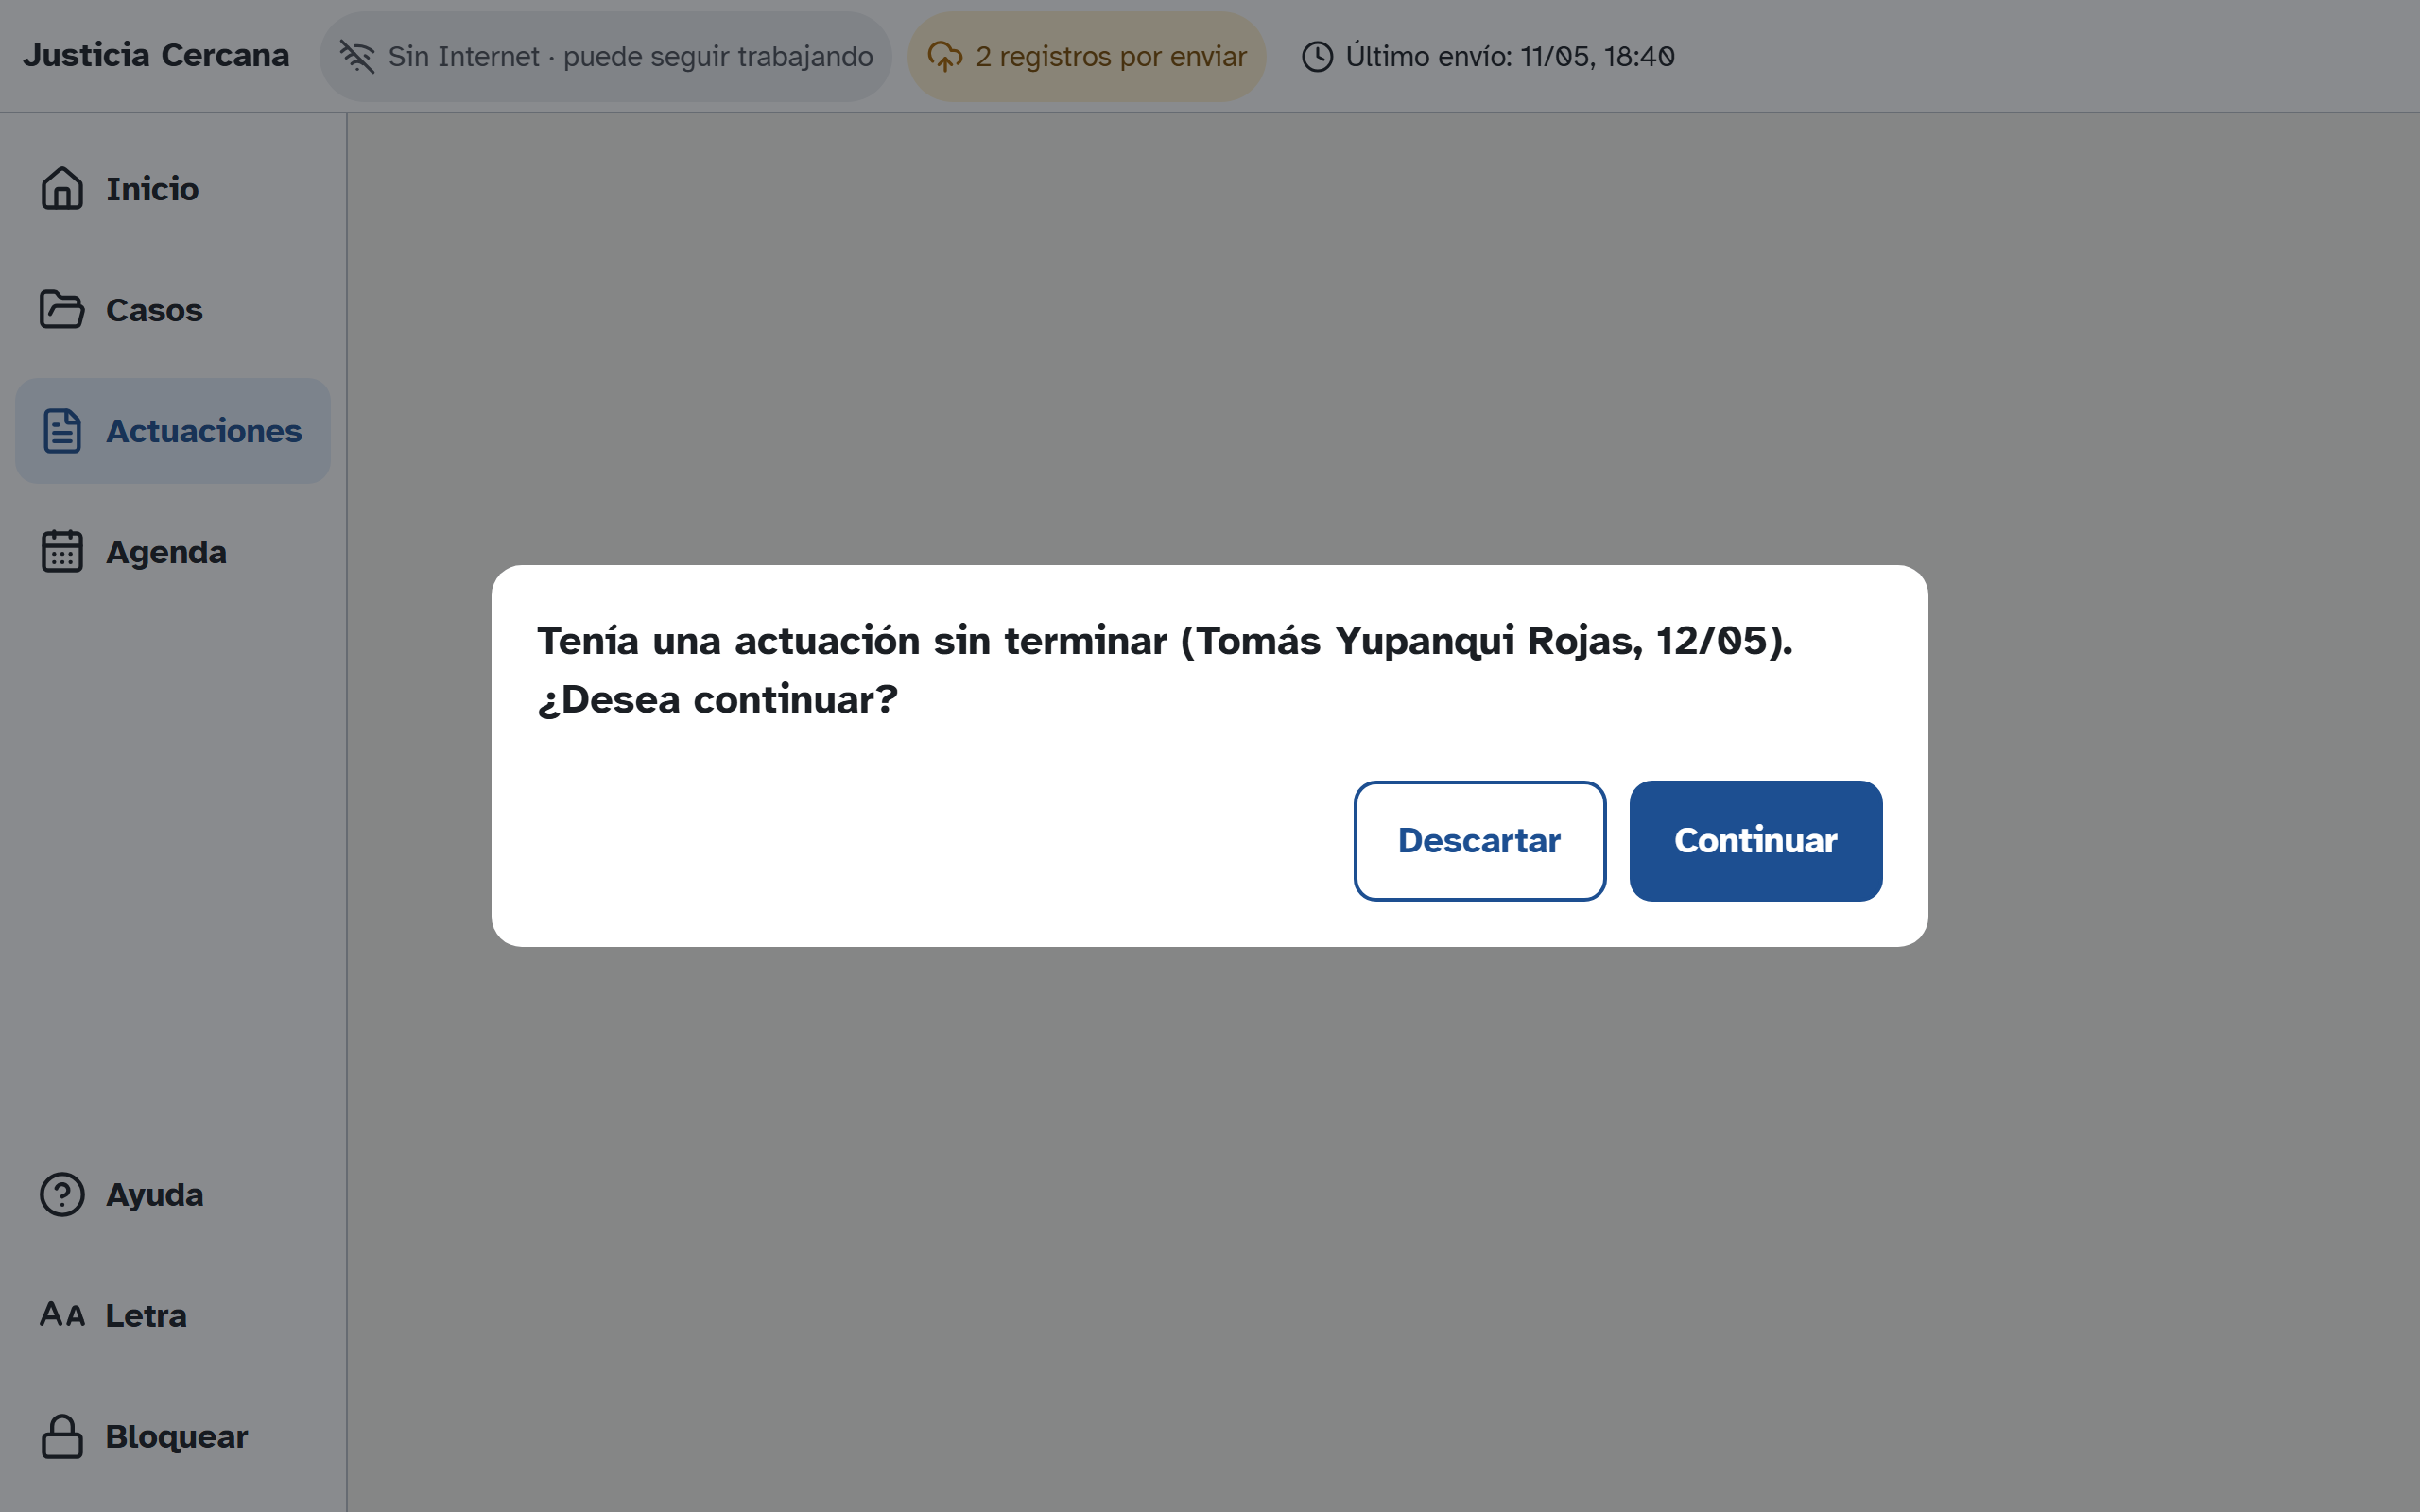
\includegraphics[width=\linewidth]{../../captures/F2-03a_recuperacion.png}\\[-2pt]{\footnotesize\raggedright\textbf{P-06 · 3.} Recuperación tras cierre inesperado: ``Tenía una actuación sin terminar. ¿Desea continuar?'' \emph{(Funcionamiento sin conexión)}\par}\end{minipage}\hfill
\begin{minipage}[t]{0.49\textwidth}\centering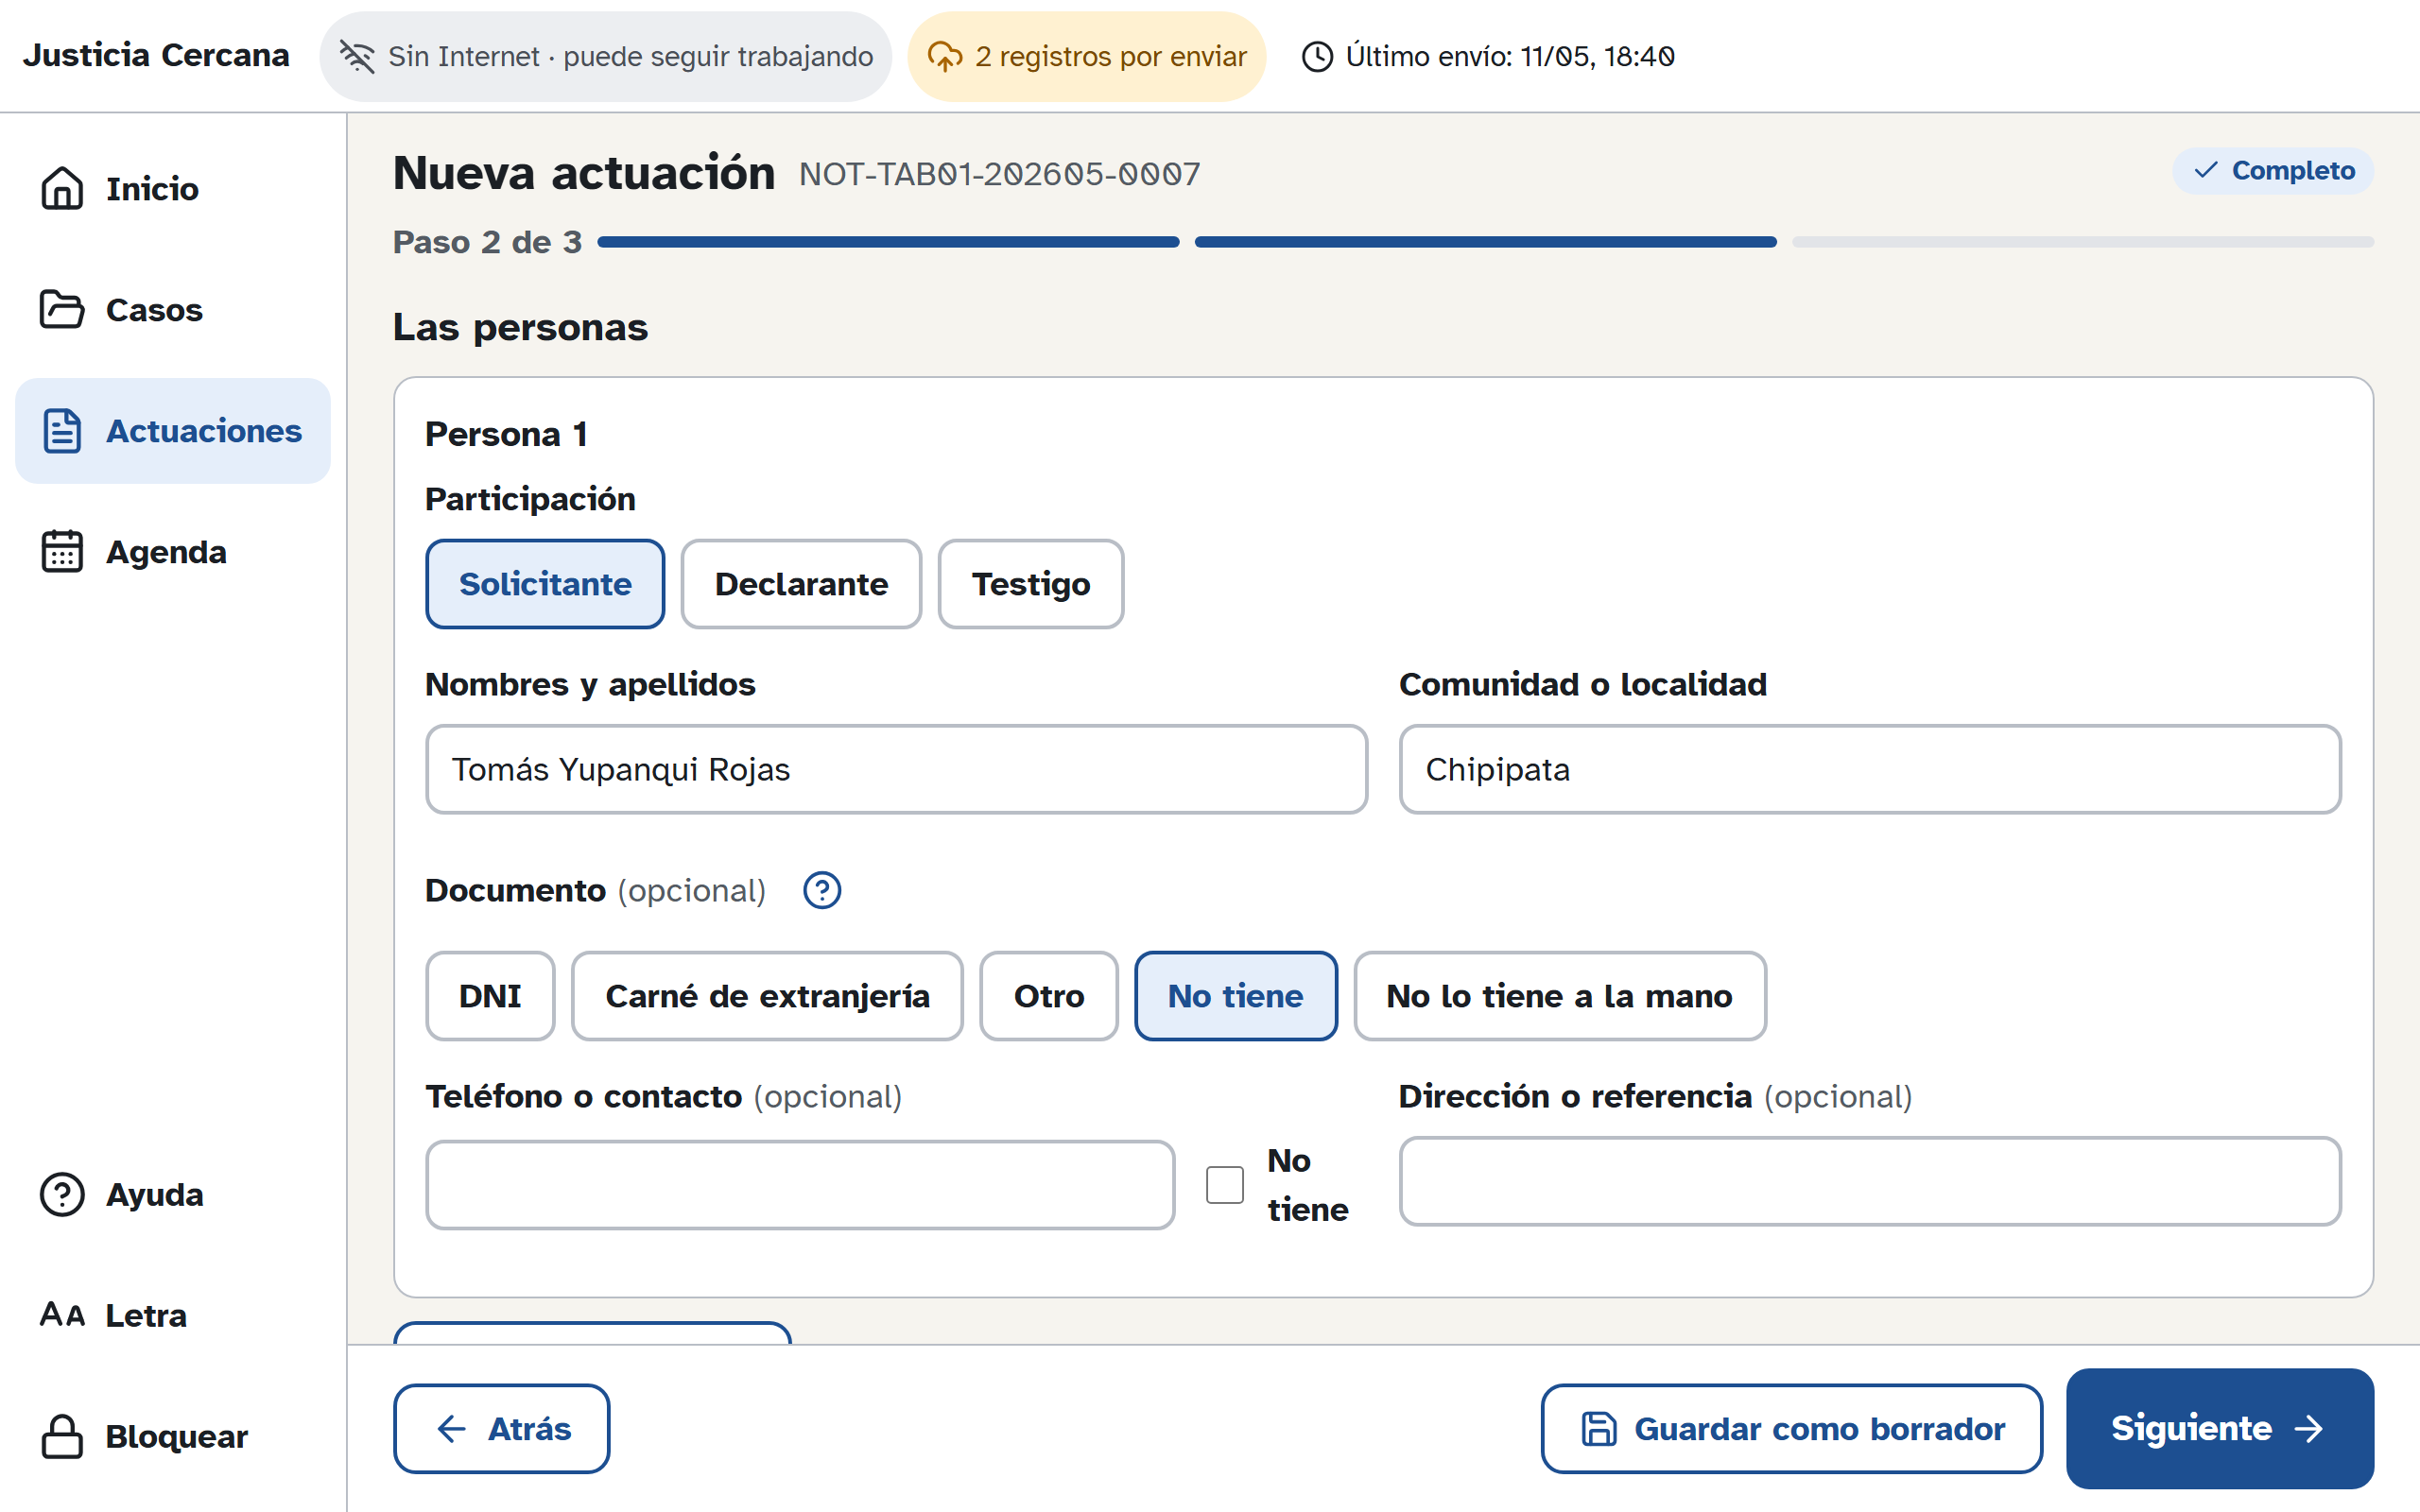
\includegraphics[width=\linewidth]{../../captures/F2-03b_continua-paso2.png}\\[-2pt]{\footnotesize\raggedright\textbf{P-06 · 3.} Continúa en el mismo paso con los datos recuperados \emph{(Funcionamiento sin conexión)}\par}\end{minipage}\par\vspace{8pt}\noindent
\begin{minipage}[t]{0.49\textwidth}\centering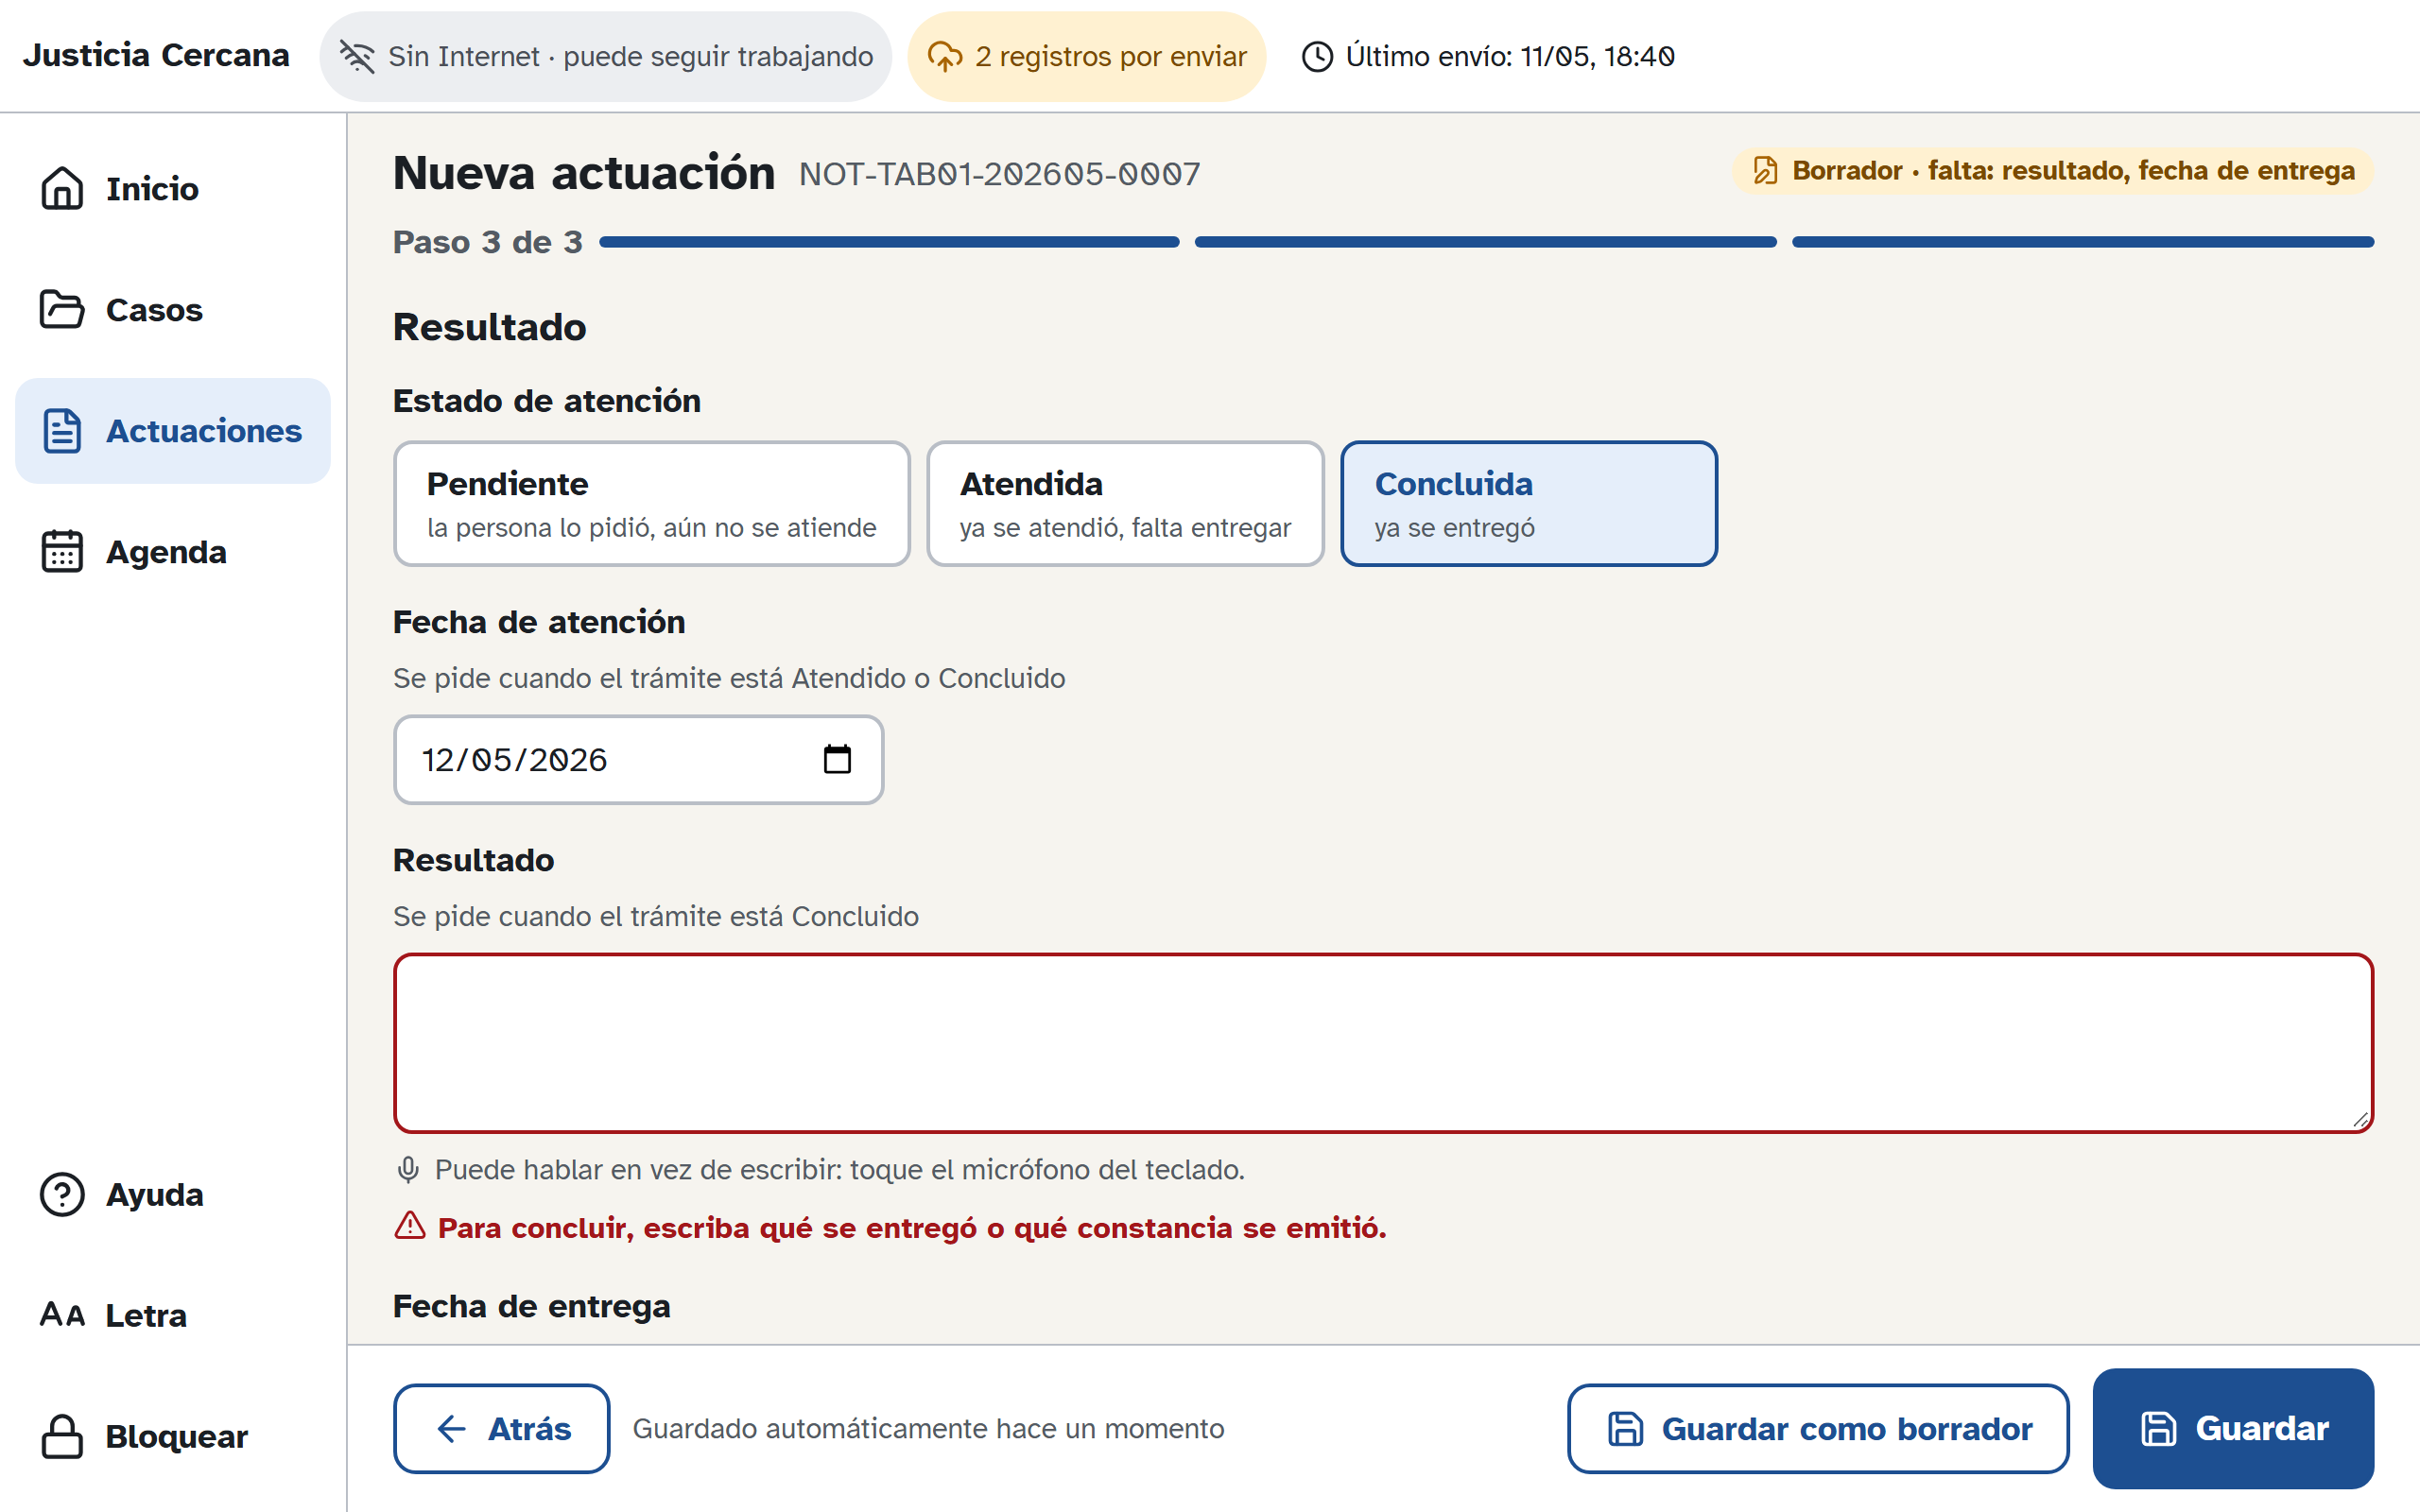
\includegraphics[width=\linewidth]{../../captures/F2-04_error-concluida-sin-resultado.png}\\[-2pt]{\footnotesize\raggedright\textbf{P-06 · 4.} Condicional: Concluida sin resultado $\rightarrow$ mensaje; líneas ``Se pide cuando…''; Borrador \emph{(Principios de diseño y heurísticas)}\par}\end{minipage}\hfill
\begin{minipage}[t]{0.49\textwidth}\centering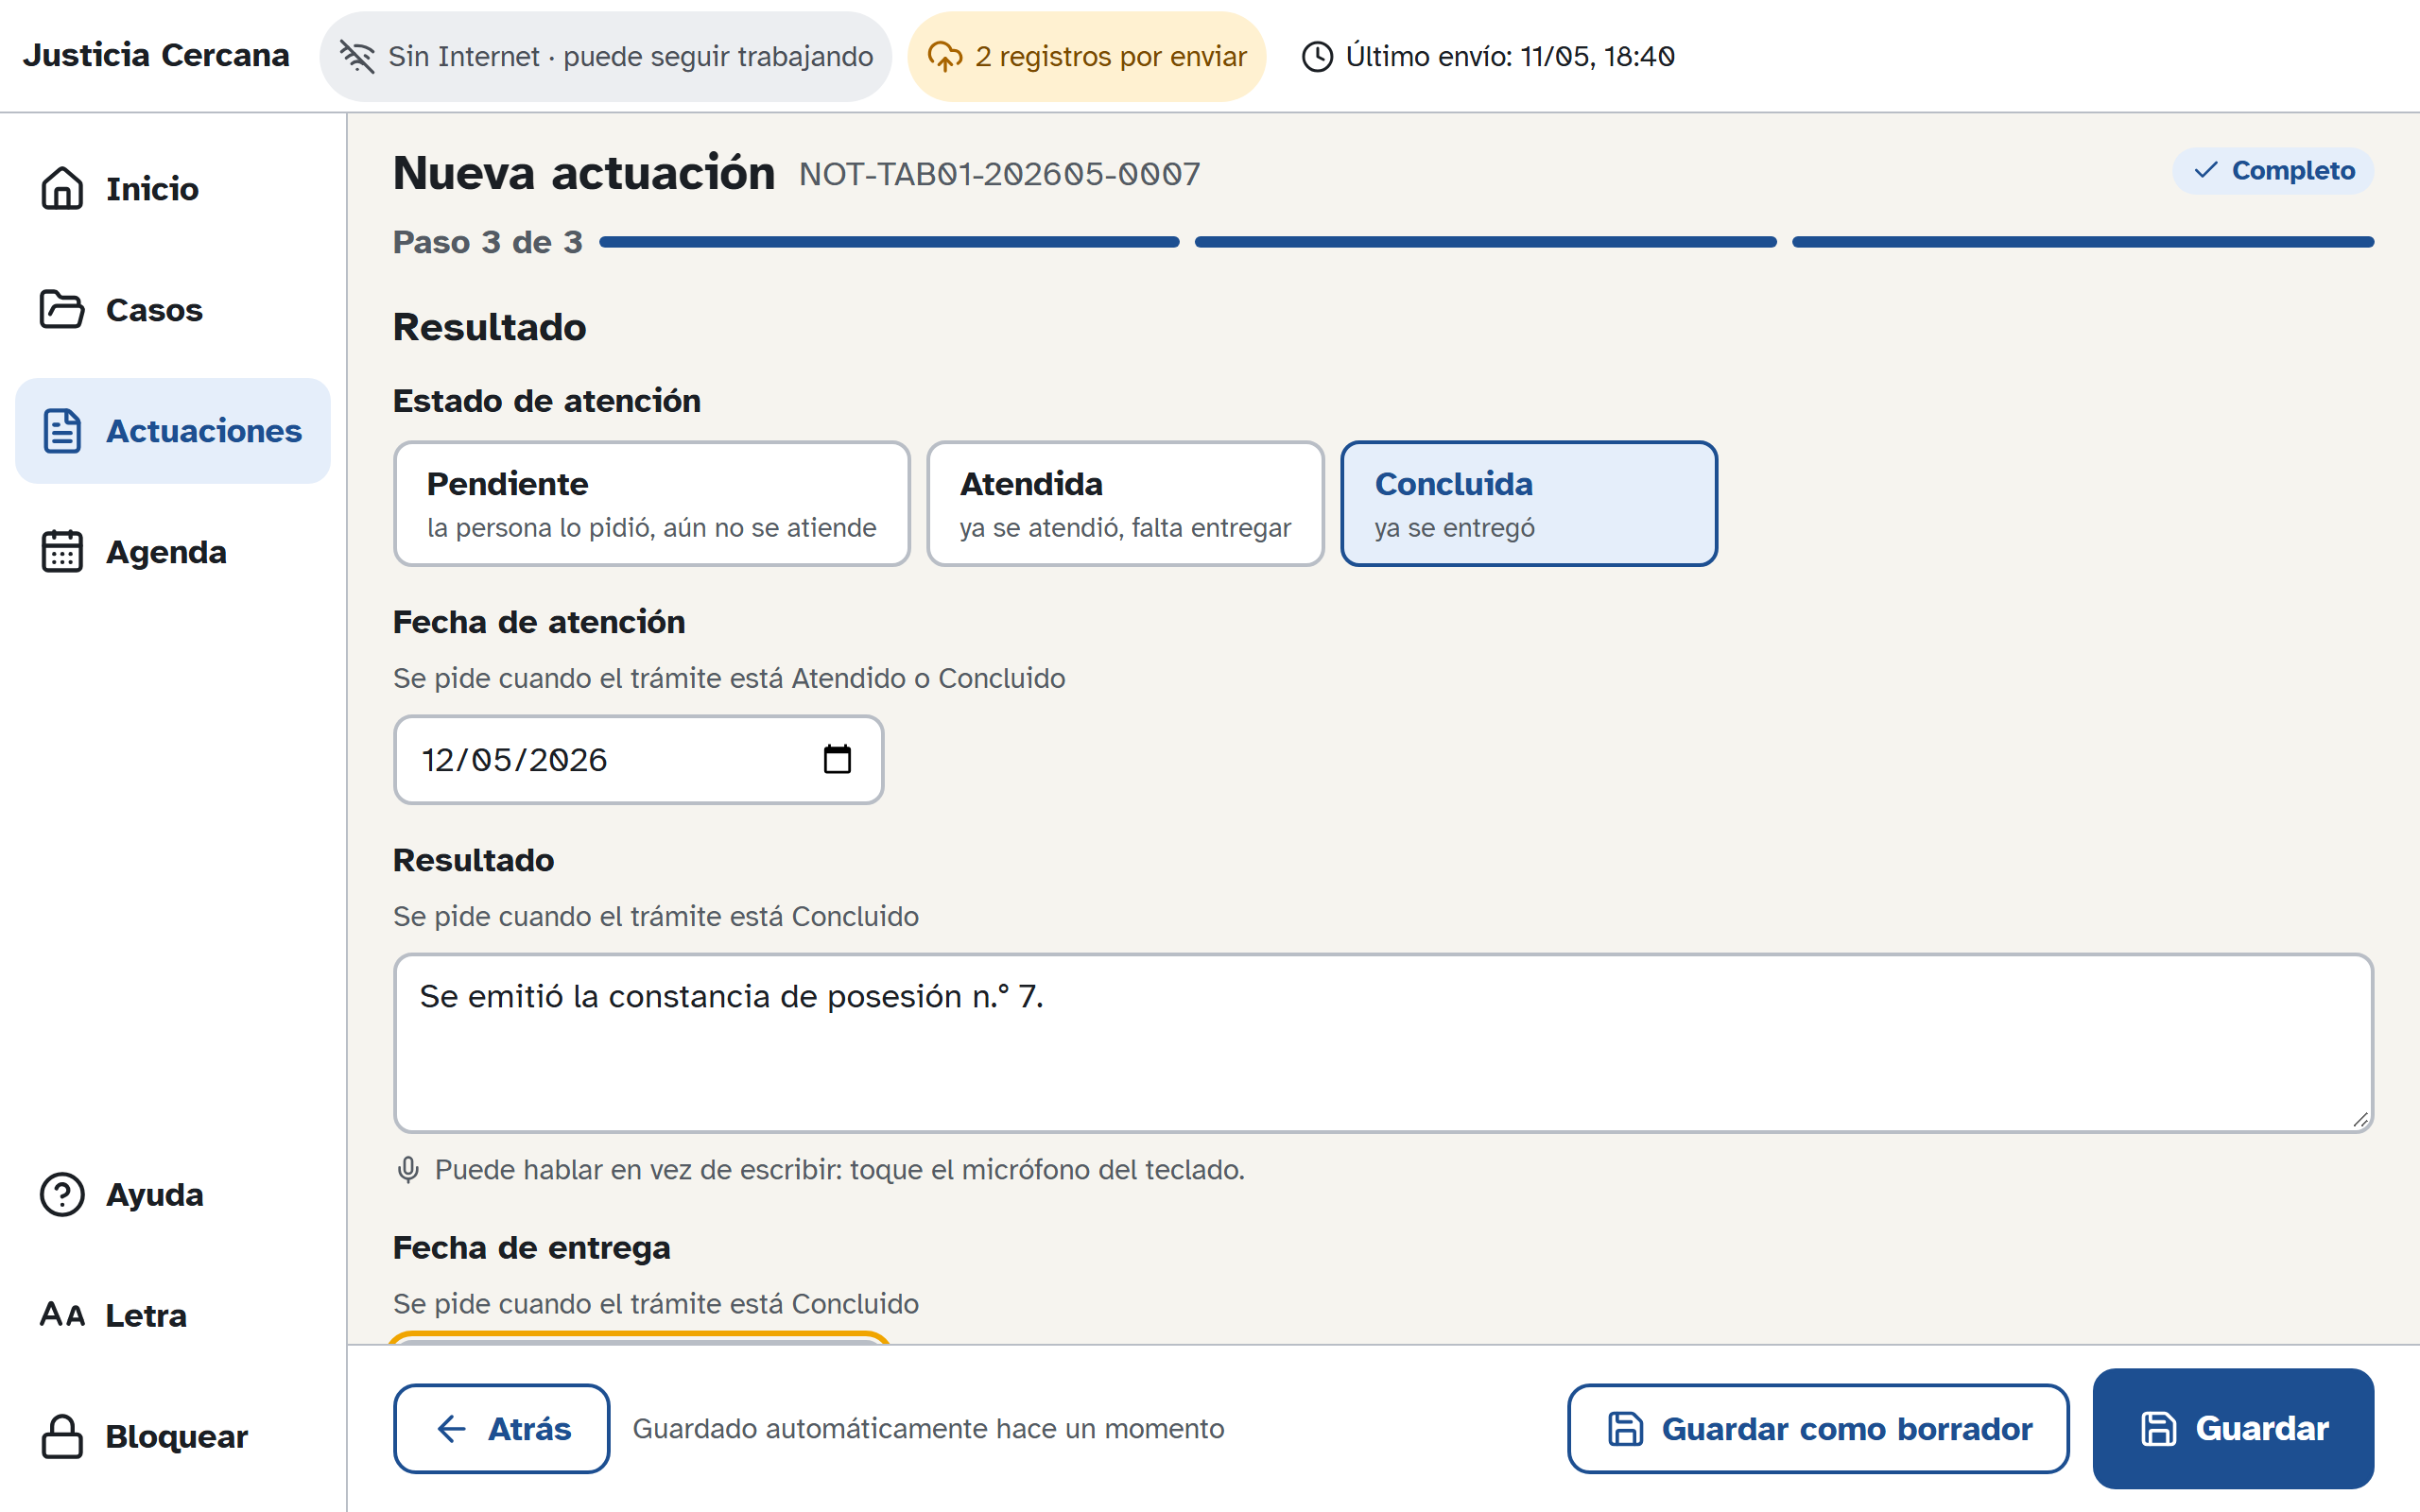
\includegraphics[width=\linewidth]{../../captures/F2-05_completo.png}\\[-2pt]{\footnotesize\raggedright\textbf{P-06 · 5.} Resultado y fecha de entrega $\rightarrow$ el registro pasa de Borrador a Completo \emph{(Cobertura y funcionamiento de los módulos)}\par}\end{minipage}\par\vspace{8pt}\noindent
\begin{minipage}[t]{0.49\textwidth}\centering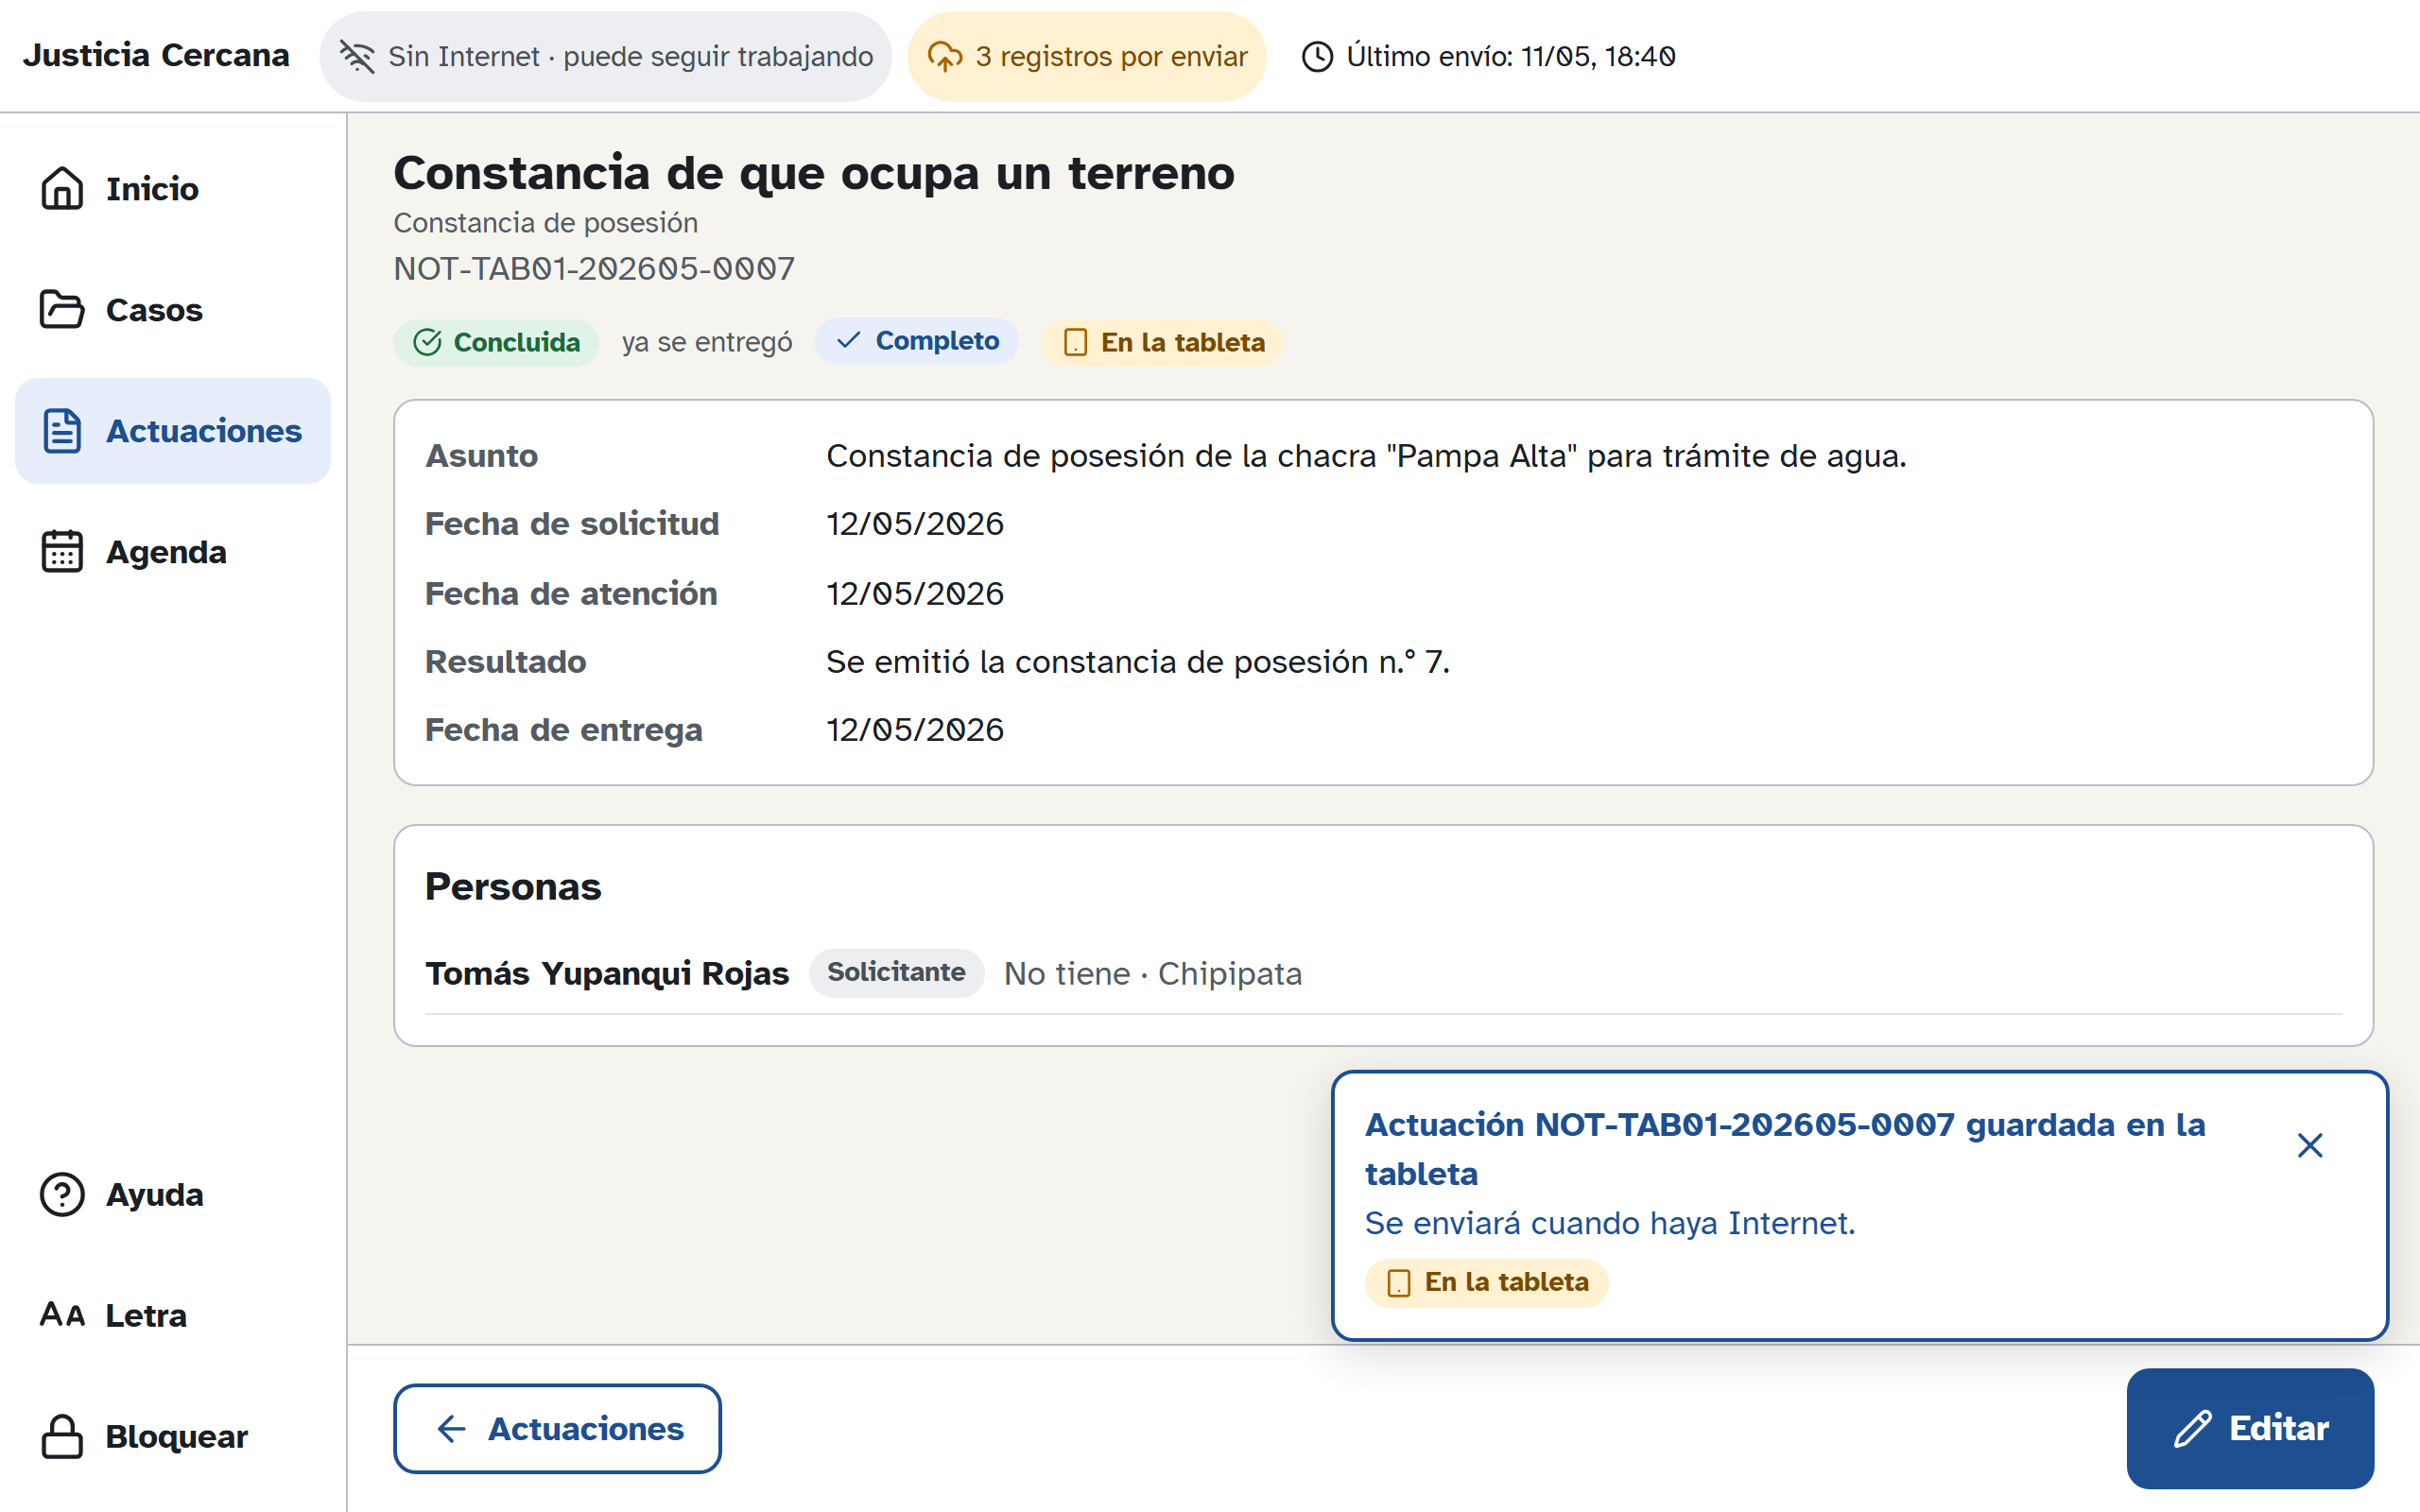
\includegraphics[width=\linewidth]{../../captures/F2-06_confirmacion-guardado.png}\\[-2pt]{\footnotesize\raggedright\textbf{P-06 · 6.} Confirmación en la tableta; barra ``3 registros por enviar'' \emph{(Funcionamiento sin conexión)}\par}\end{minipage}\hfill
\par\vspace{4pt}
\subsection*{Flujo 3}
\noindent
\begin{minipage}[t]{0.49\textwidth}\centering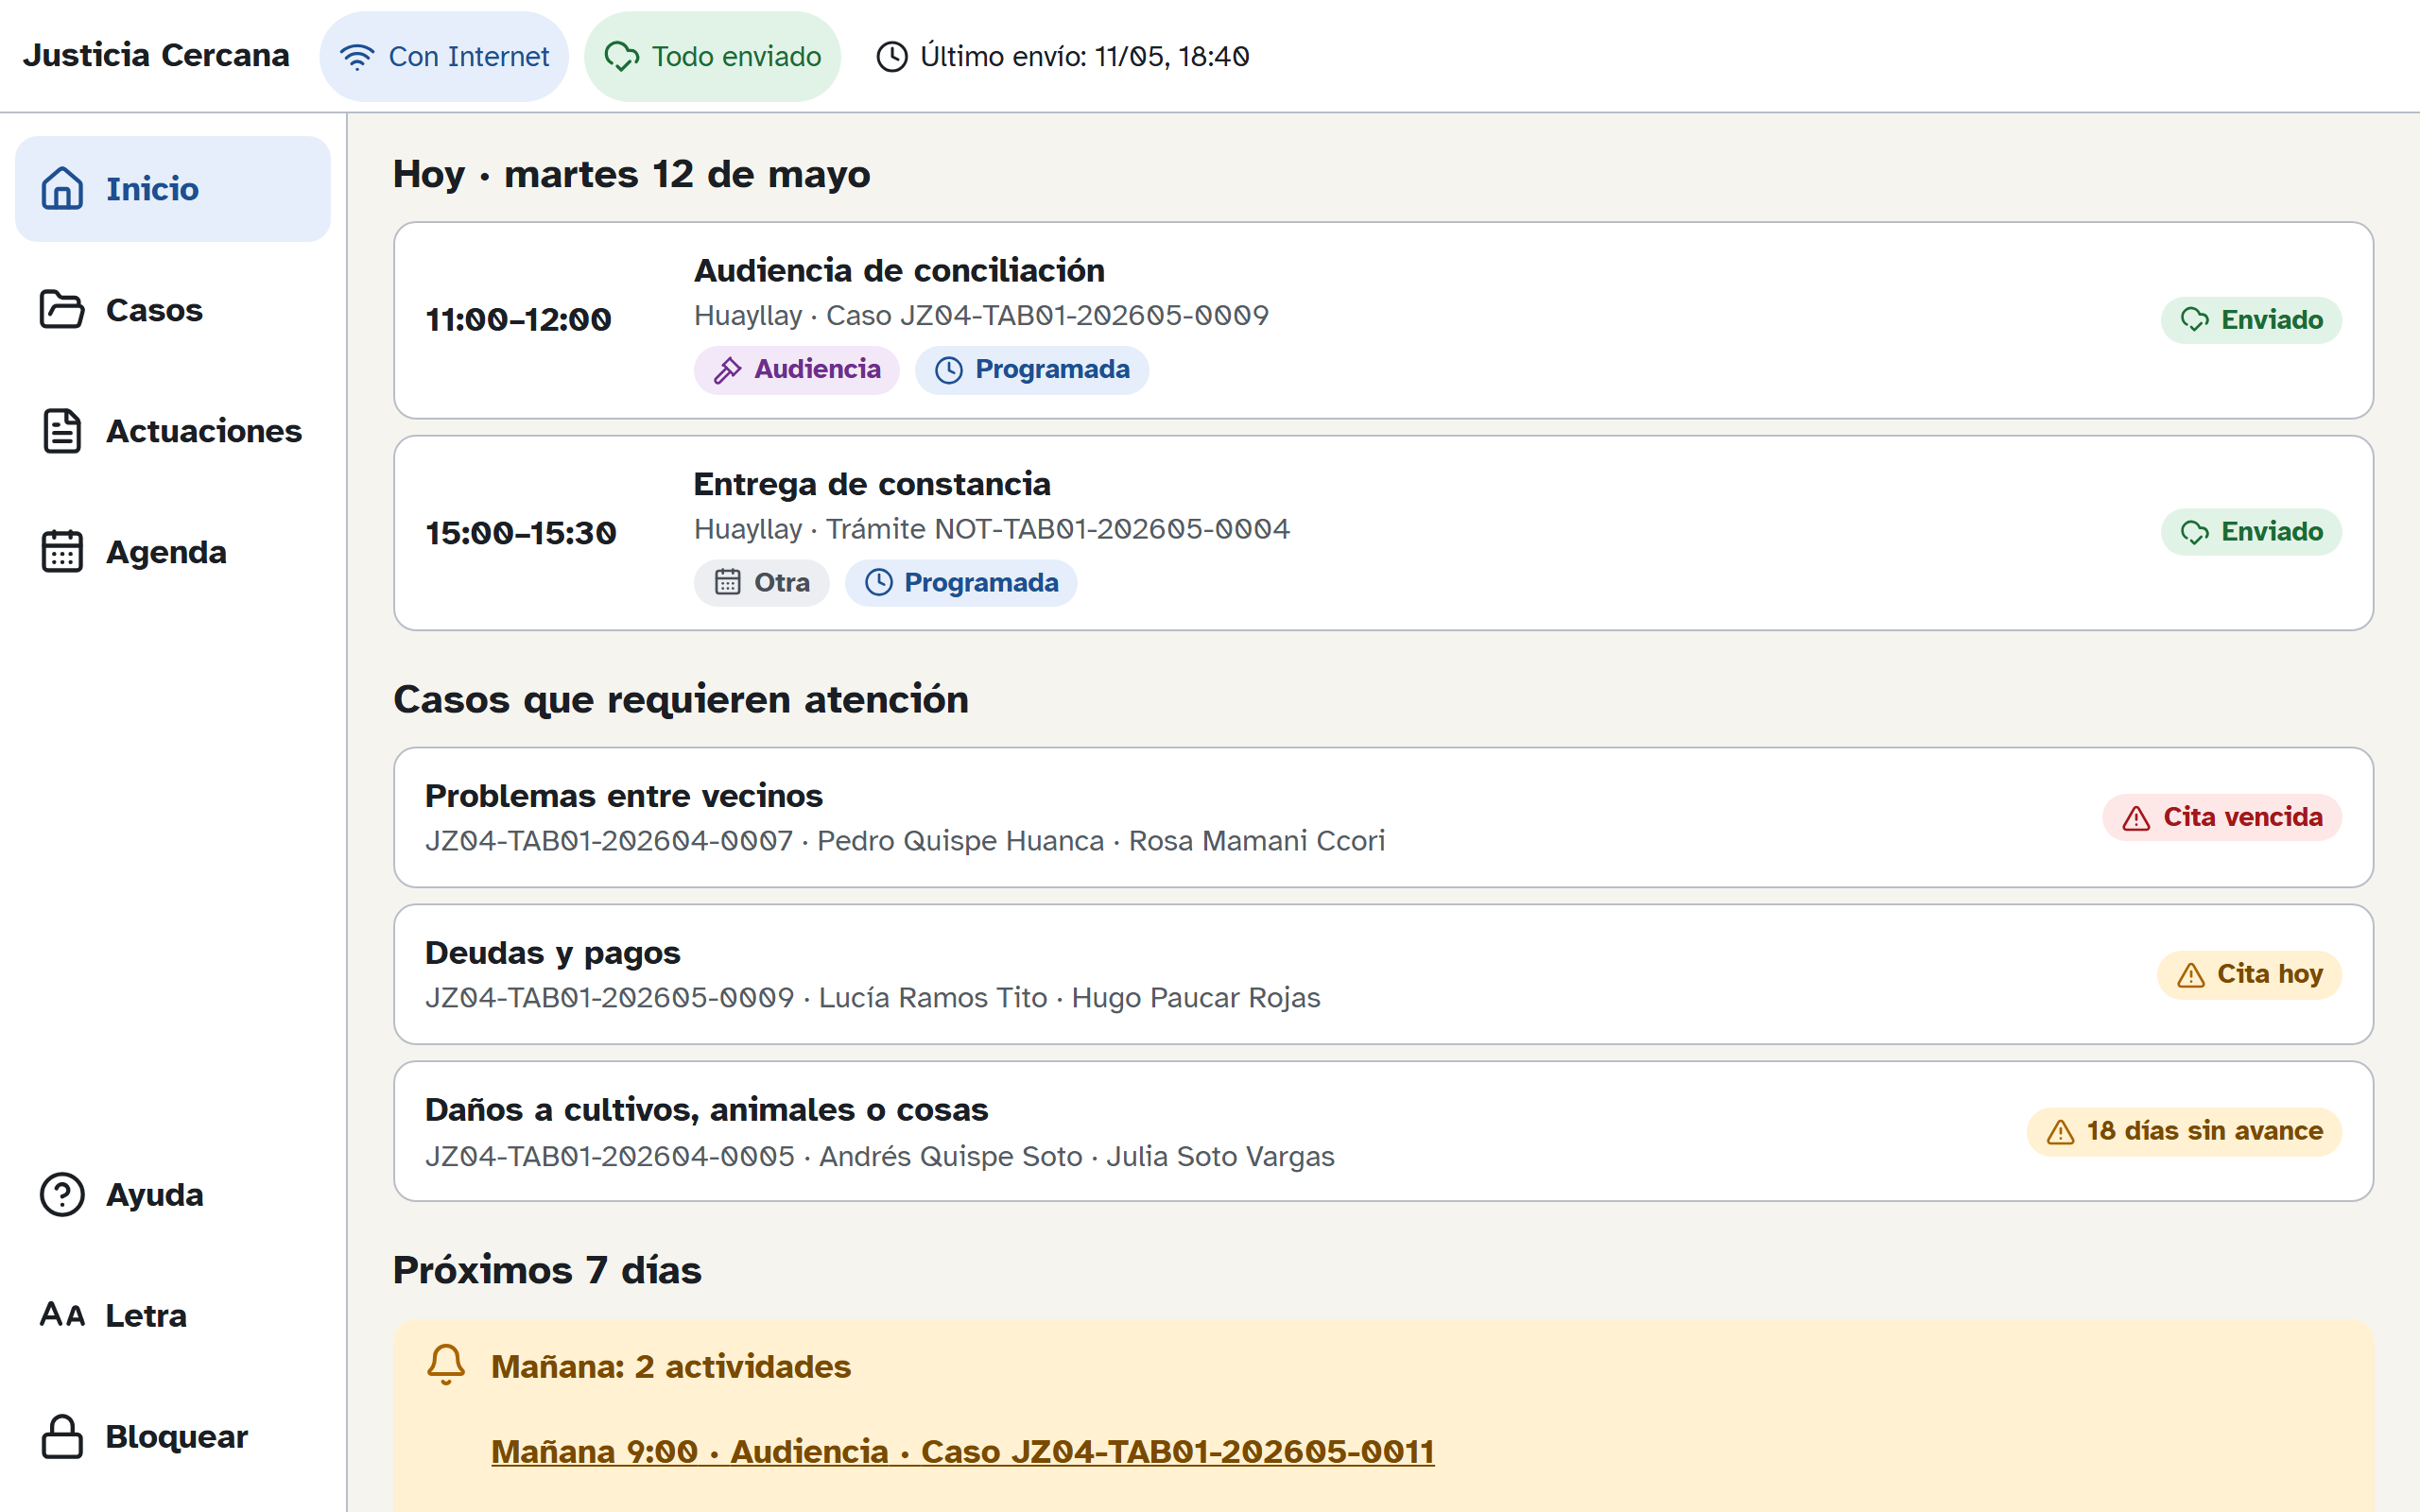
\includegraphics[width=\linewidth]{../../captures/F3-01_inicio-manana.png}\\[-2pt]{\footnotesize\raggedright\textbf{P-01 · 1.} Aviso de próximas ``Mañana: 2 actividades'' en Inicio \emph{(Cobertura y funcionamiento de los módulos)}\par}\end{minipage}\hfill
\begin{minipage}[t]{0.49\textwidth}\centering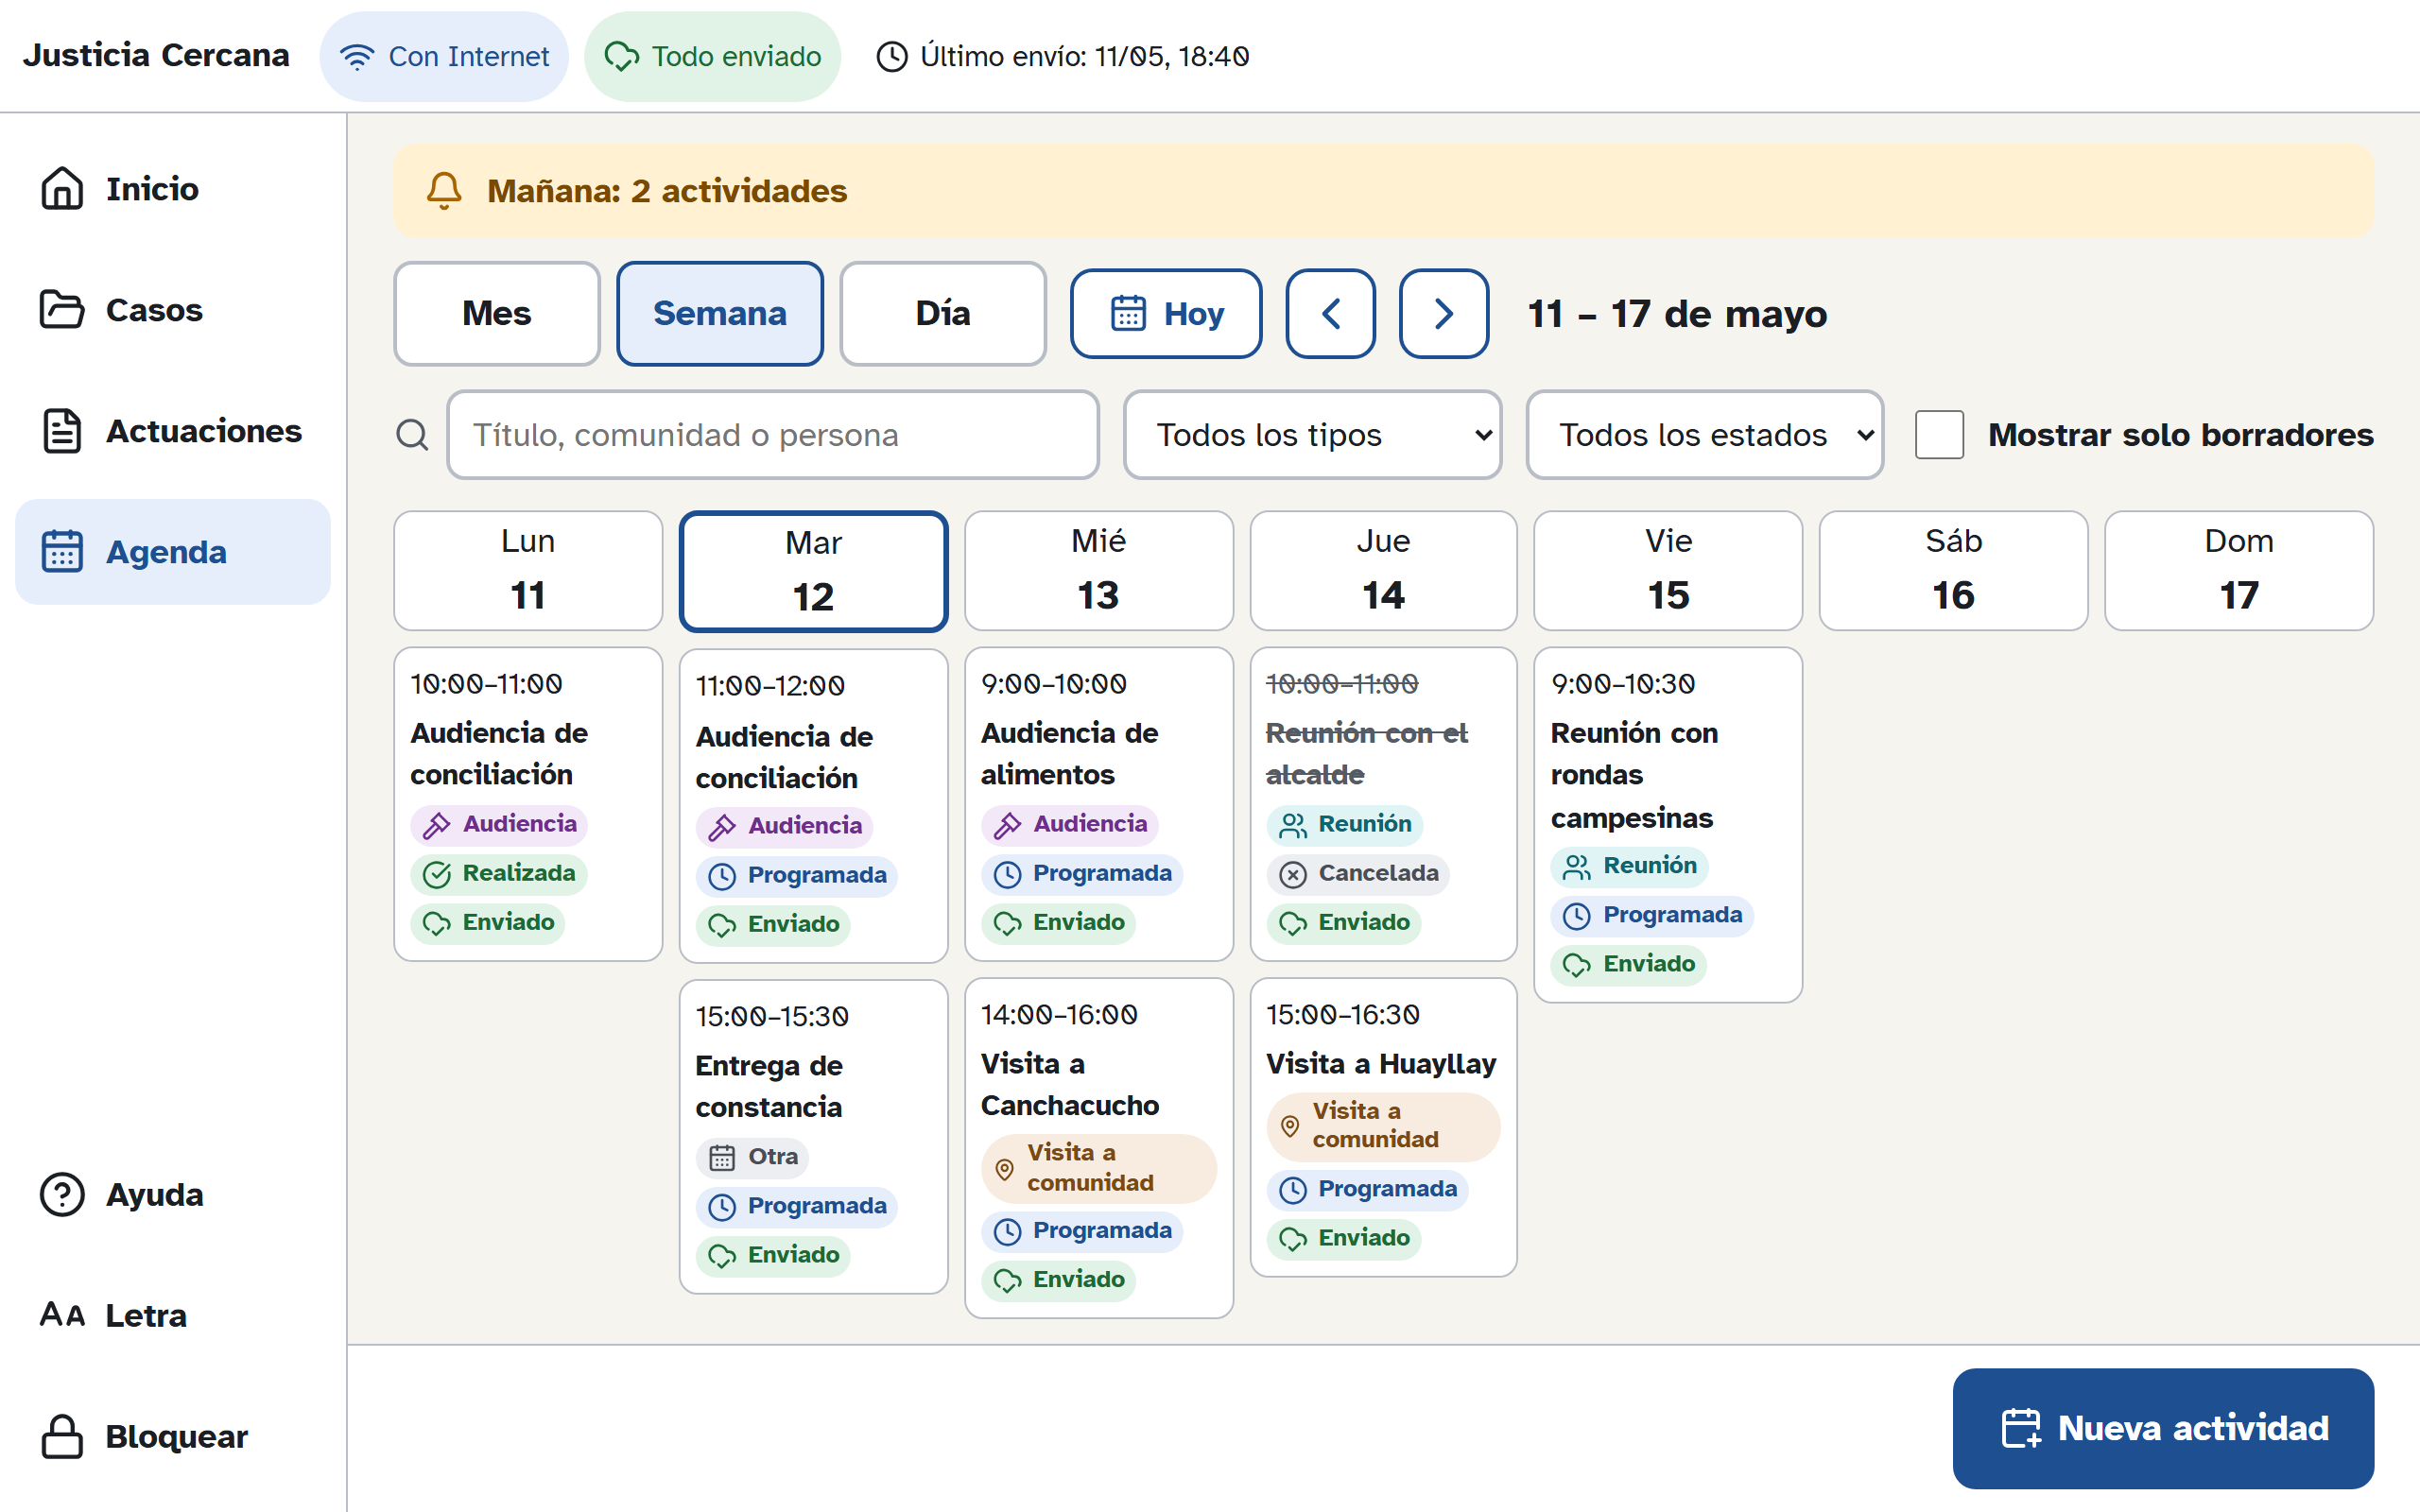
\includegraphics[width=\linewidth]{../../captures/F3-02_agenda-semana.png}\\[-2pt]{\footnotesize\raggedright\textbf{P-07 · 2.} Vista Semana: categorías con color + ícono + texto y estados \emph{(Cobertura y funcionamiento de los módulos)}\par}\end{minipage}\par\vspace{8pt}\noindent
\begin{minipage}[t]{0.49\textwidth}\centering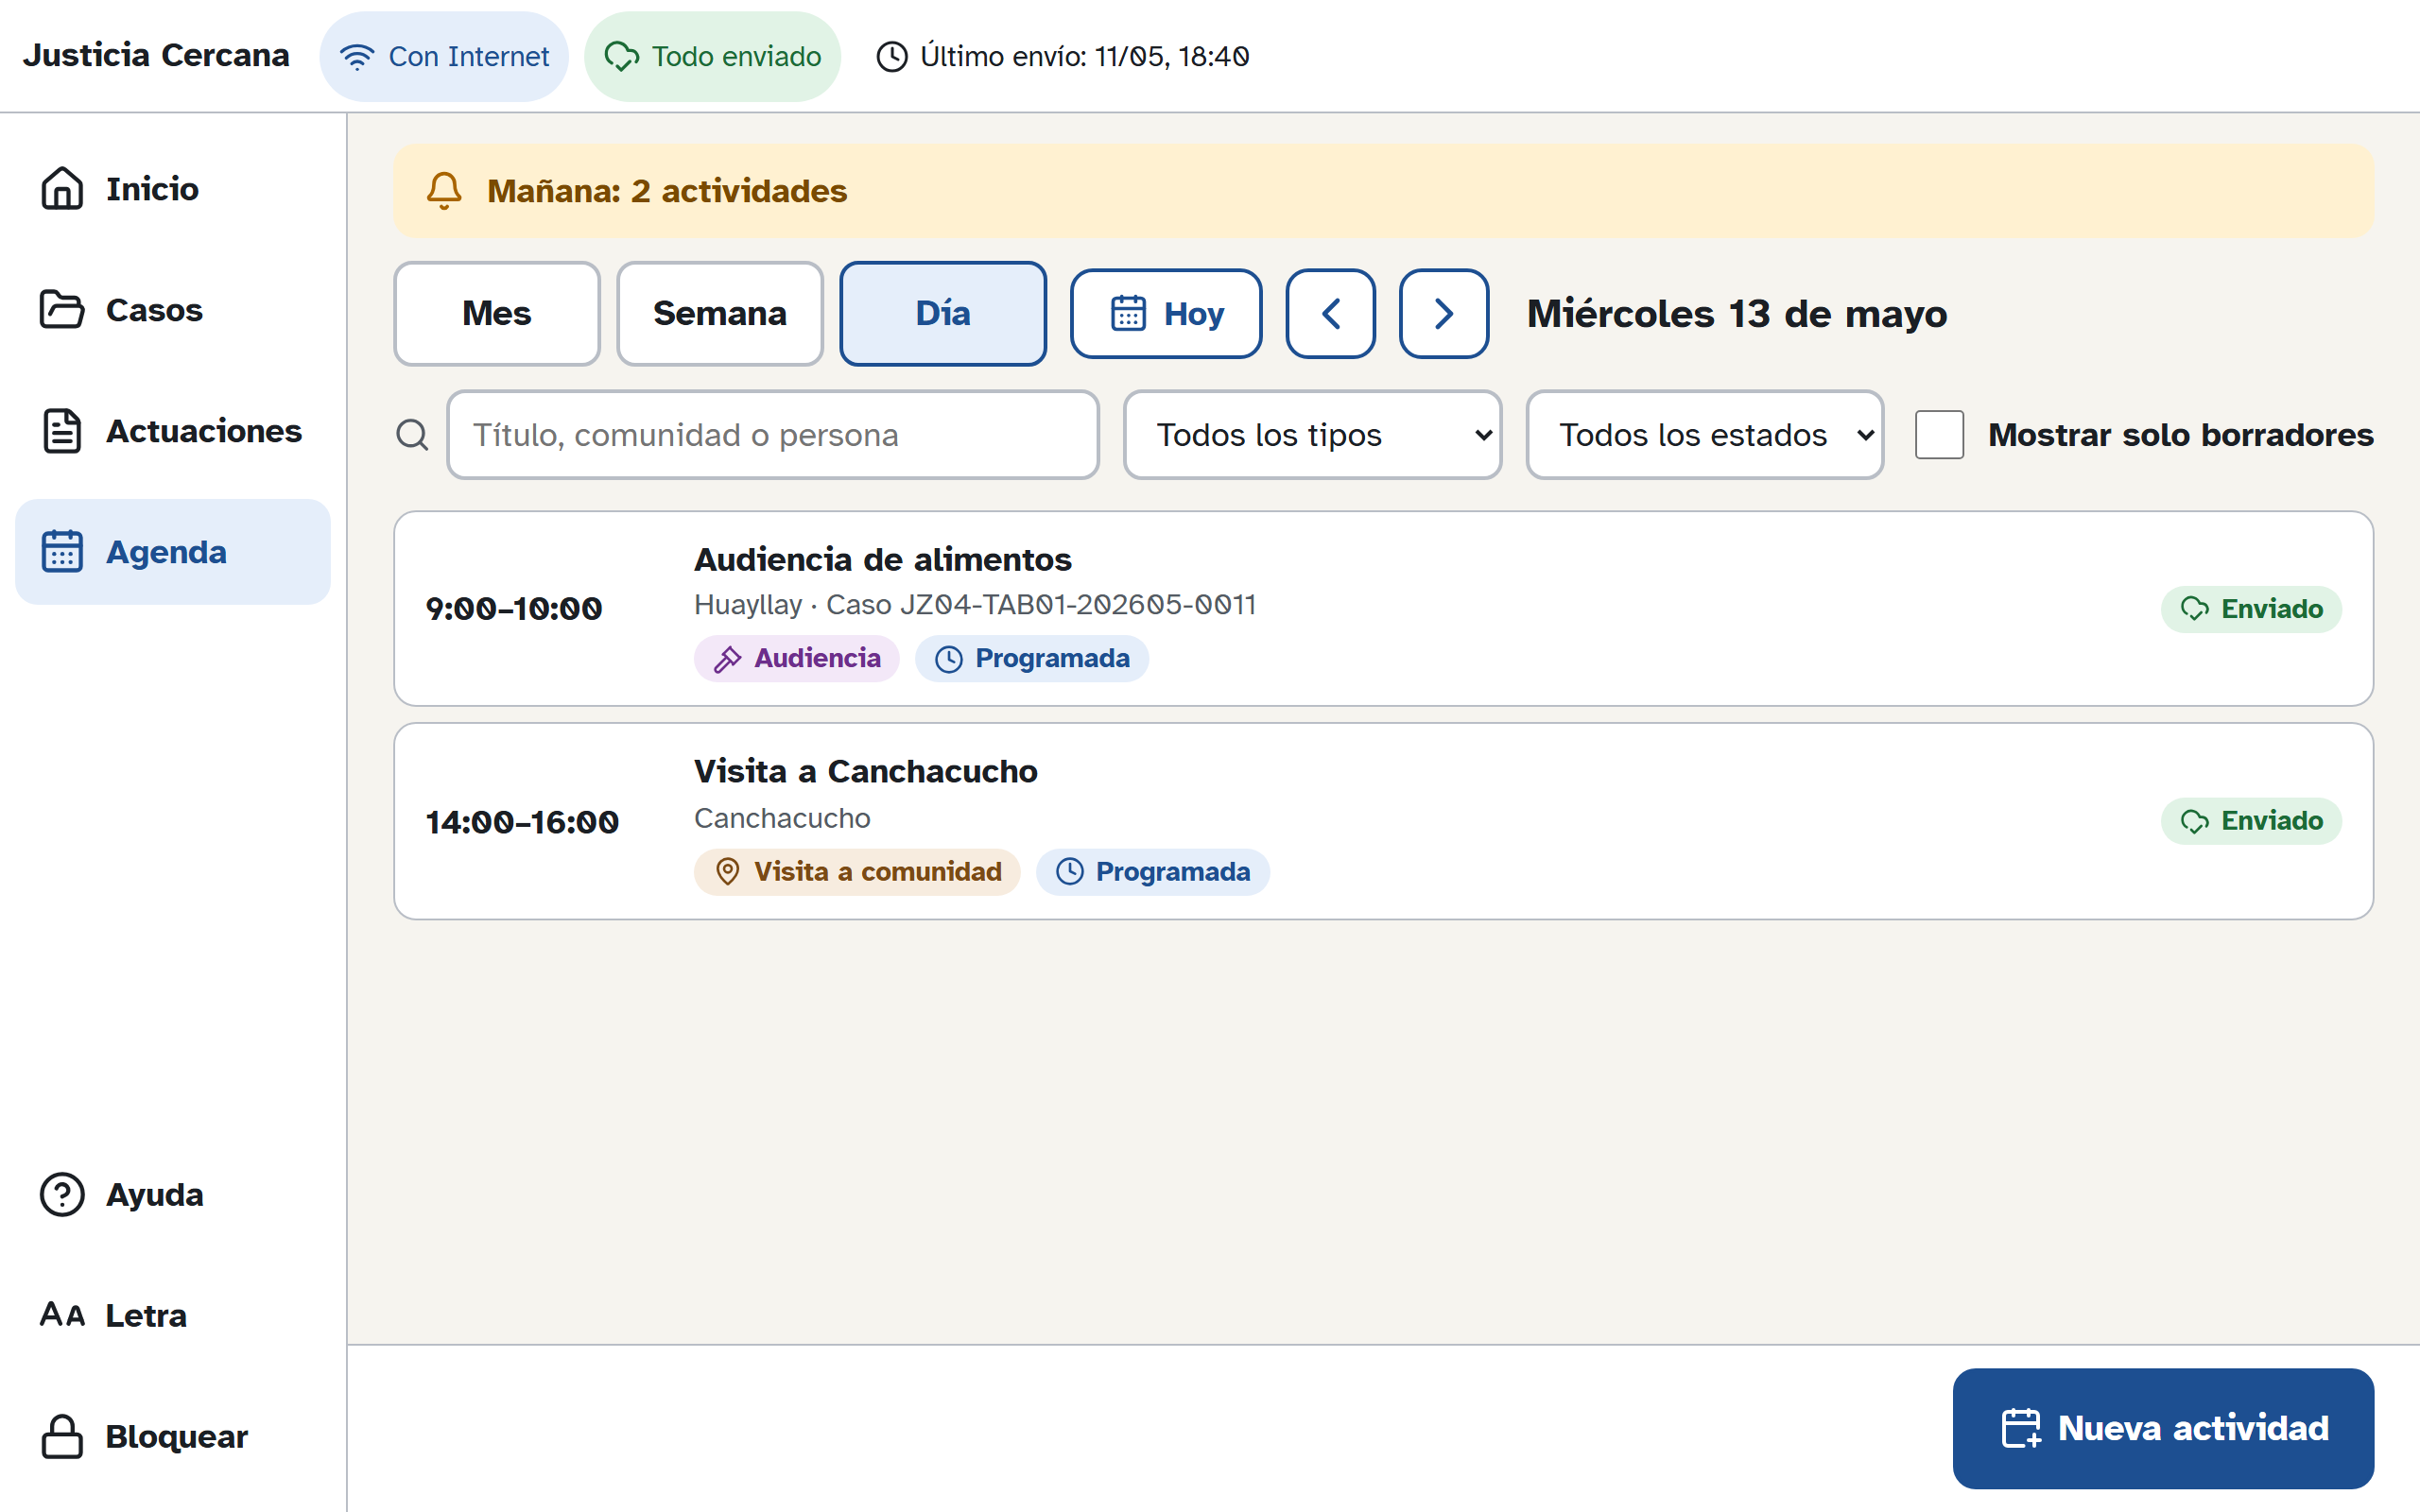
\includegraphics[width=\linewidth]{../../captures/F3-03a_agenda-dia-miercoles.png}\\[-2pt]{\footnotesize\raggedright\textbf{P-07 · 3.} Vista Día del miércoles con detalle \emph{(Cobertura y funcionamiento de los módulos)}\par}\end{minipage}\hfill
\begin{minipage}[t]{0.49\textwidth}\centering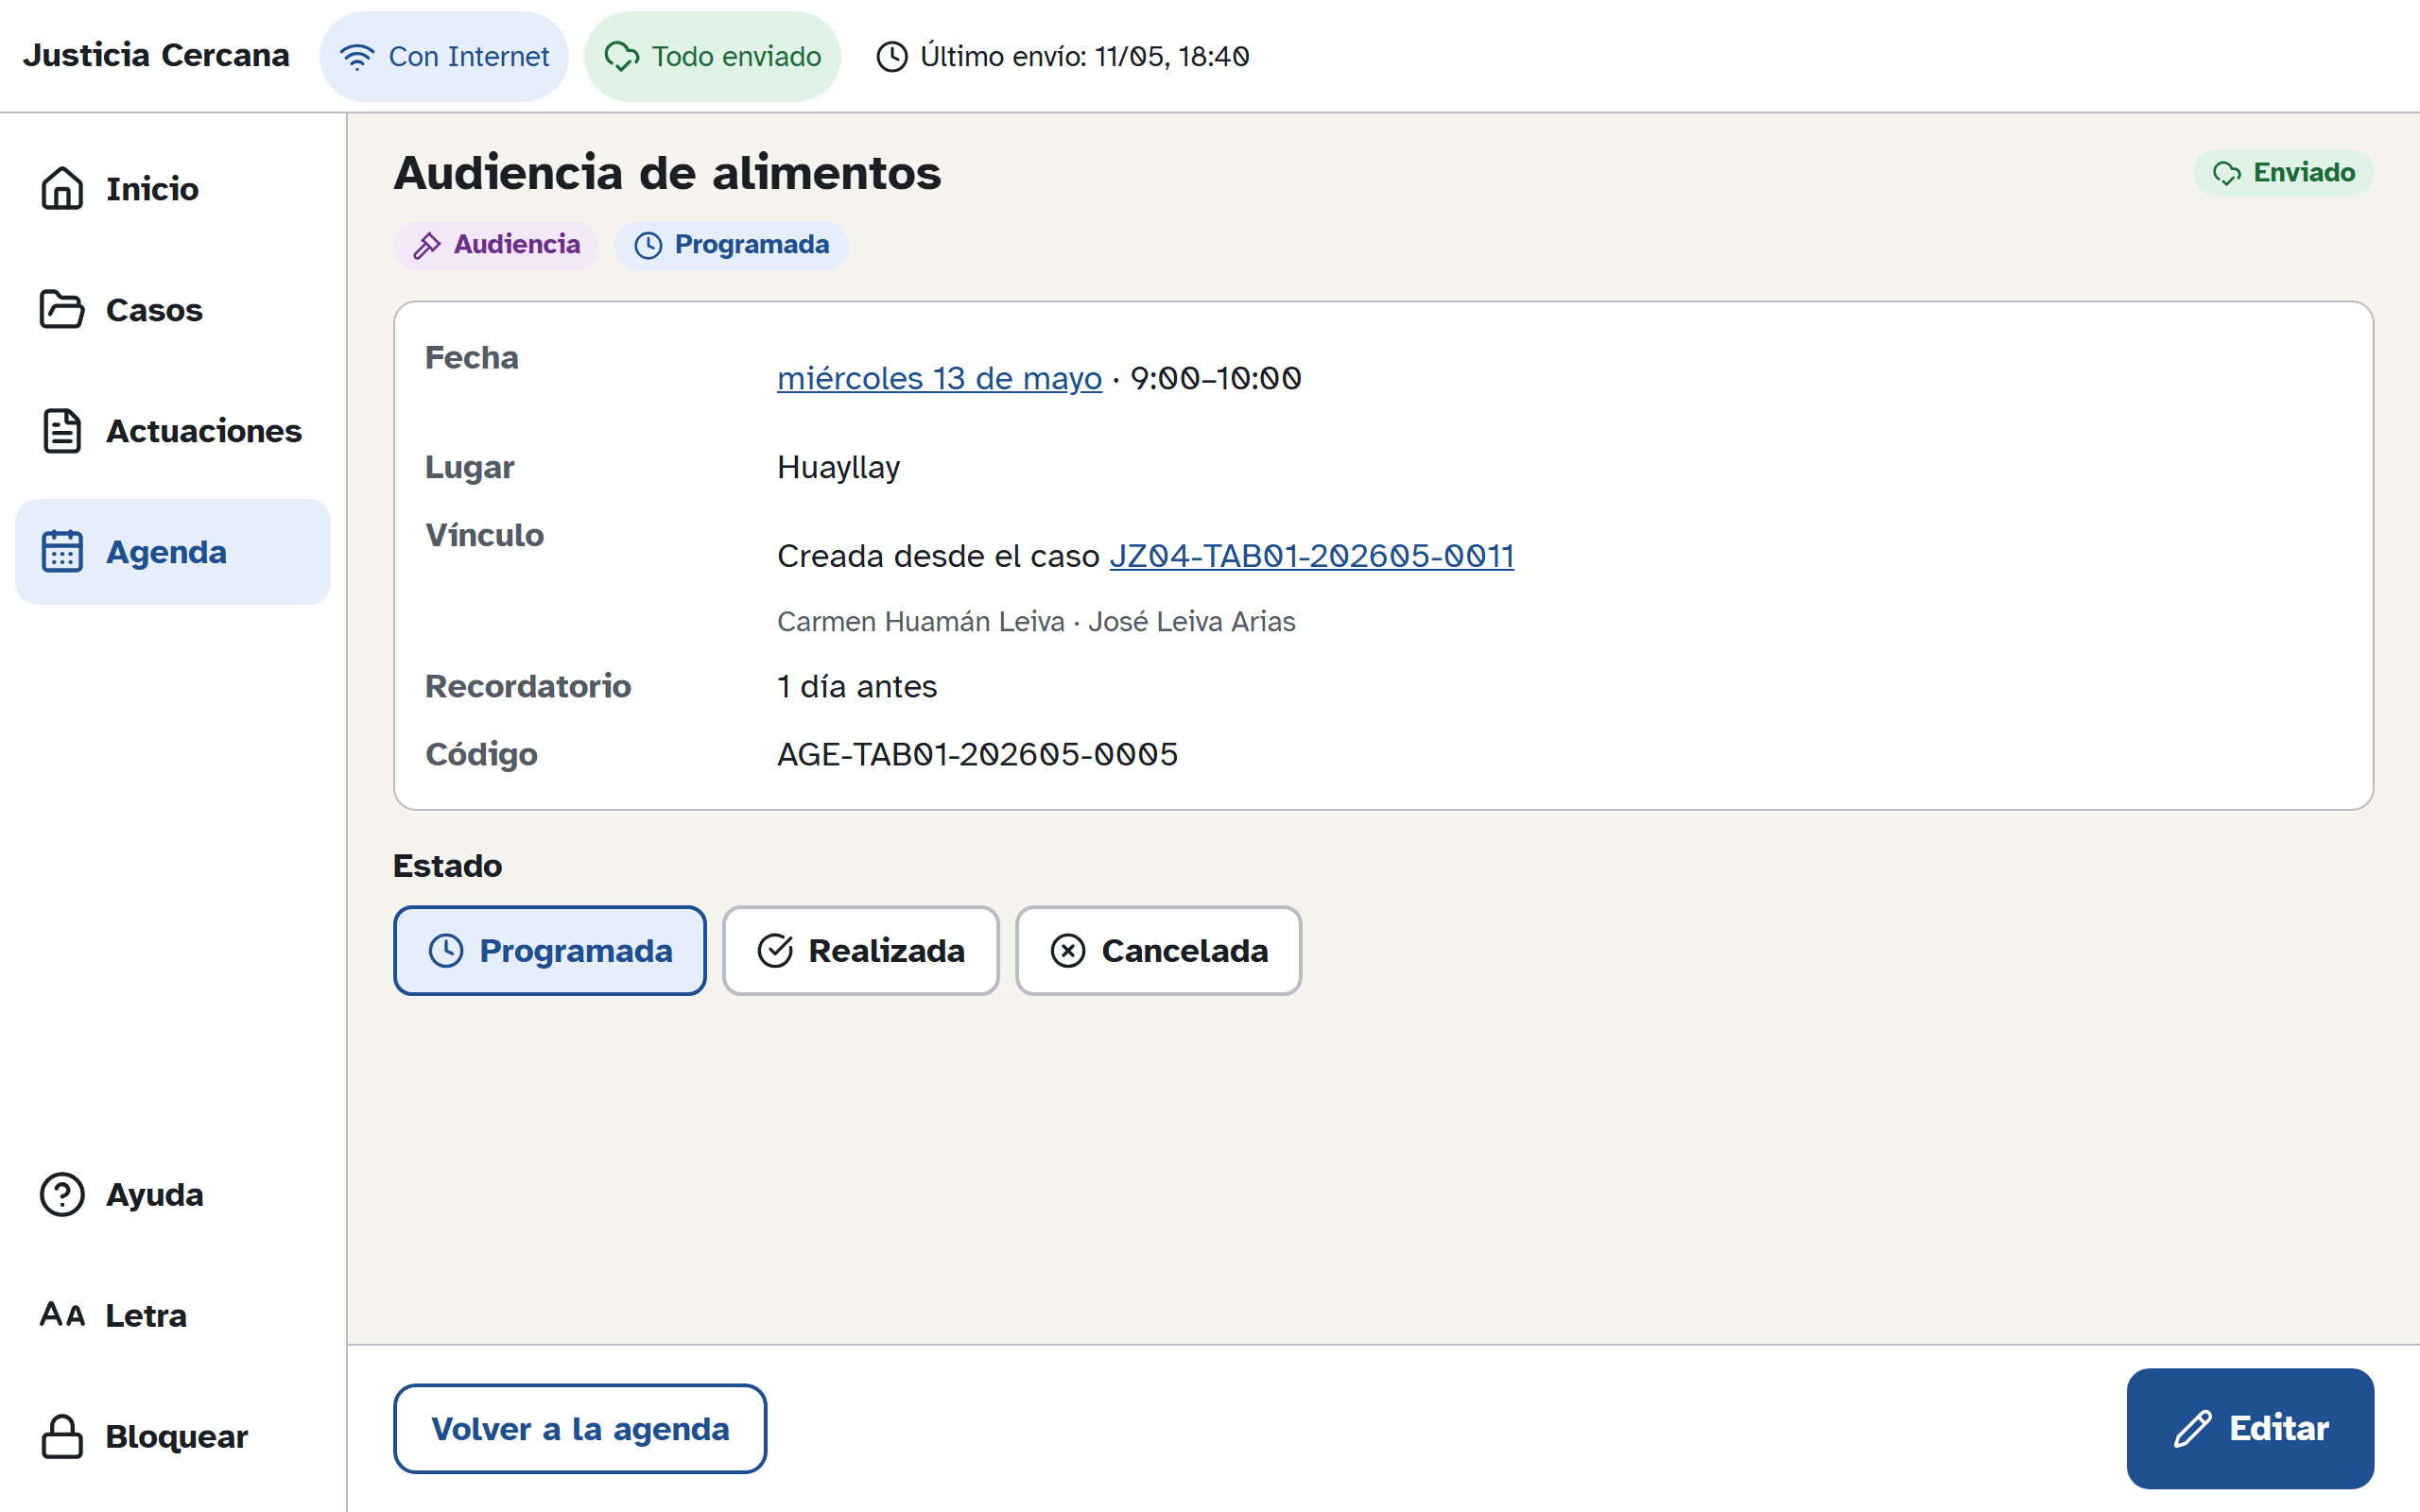
\includegraphics[width=\linewidth]{../../captures/F3-03b_detalle-vinculo-caso.png}\\[-2pt]{\footnotesize\raggedright\textbf{P-08 · 3.} Detalle de la actividad con vínculo al caso \emph{(Cobertura y funcionamiento de los módulos)}\par}\end{minipage}\par\vspace{8pt}\noindent
\par\vspace{4pt}
\subsection*{Flujo 4}
\noindent
\begin{minipage}[t]{0.49\textwidth}\centering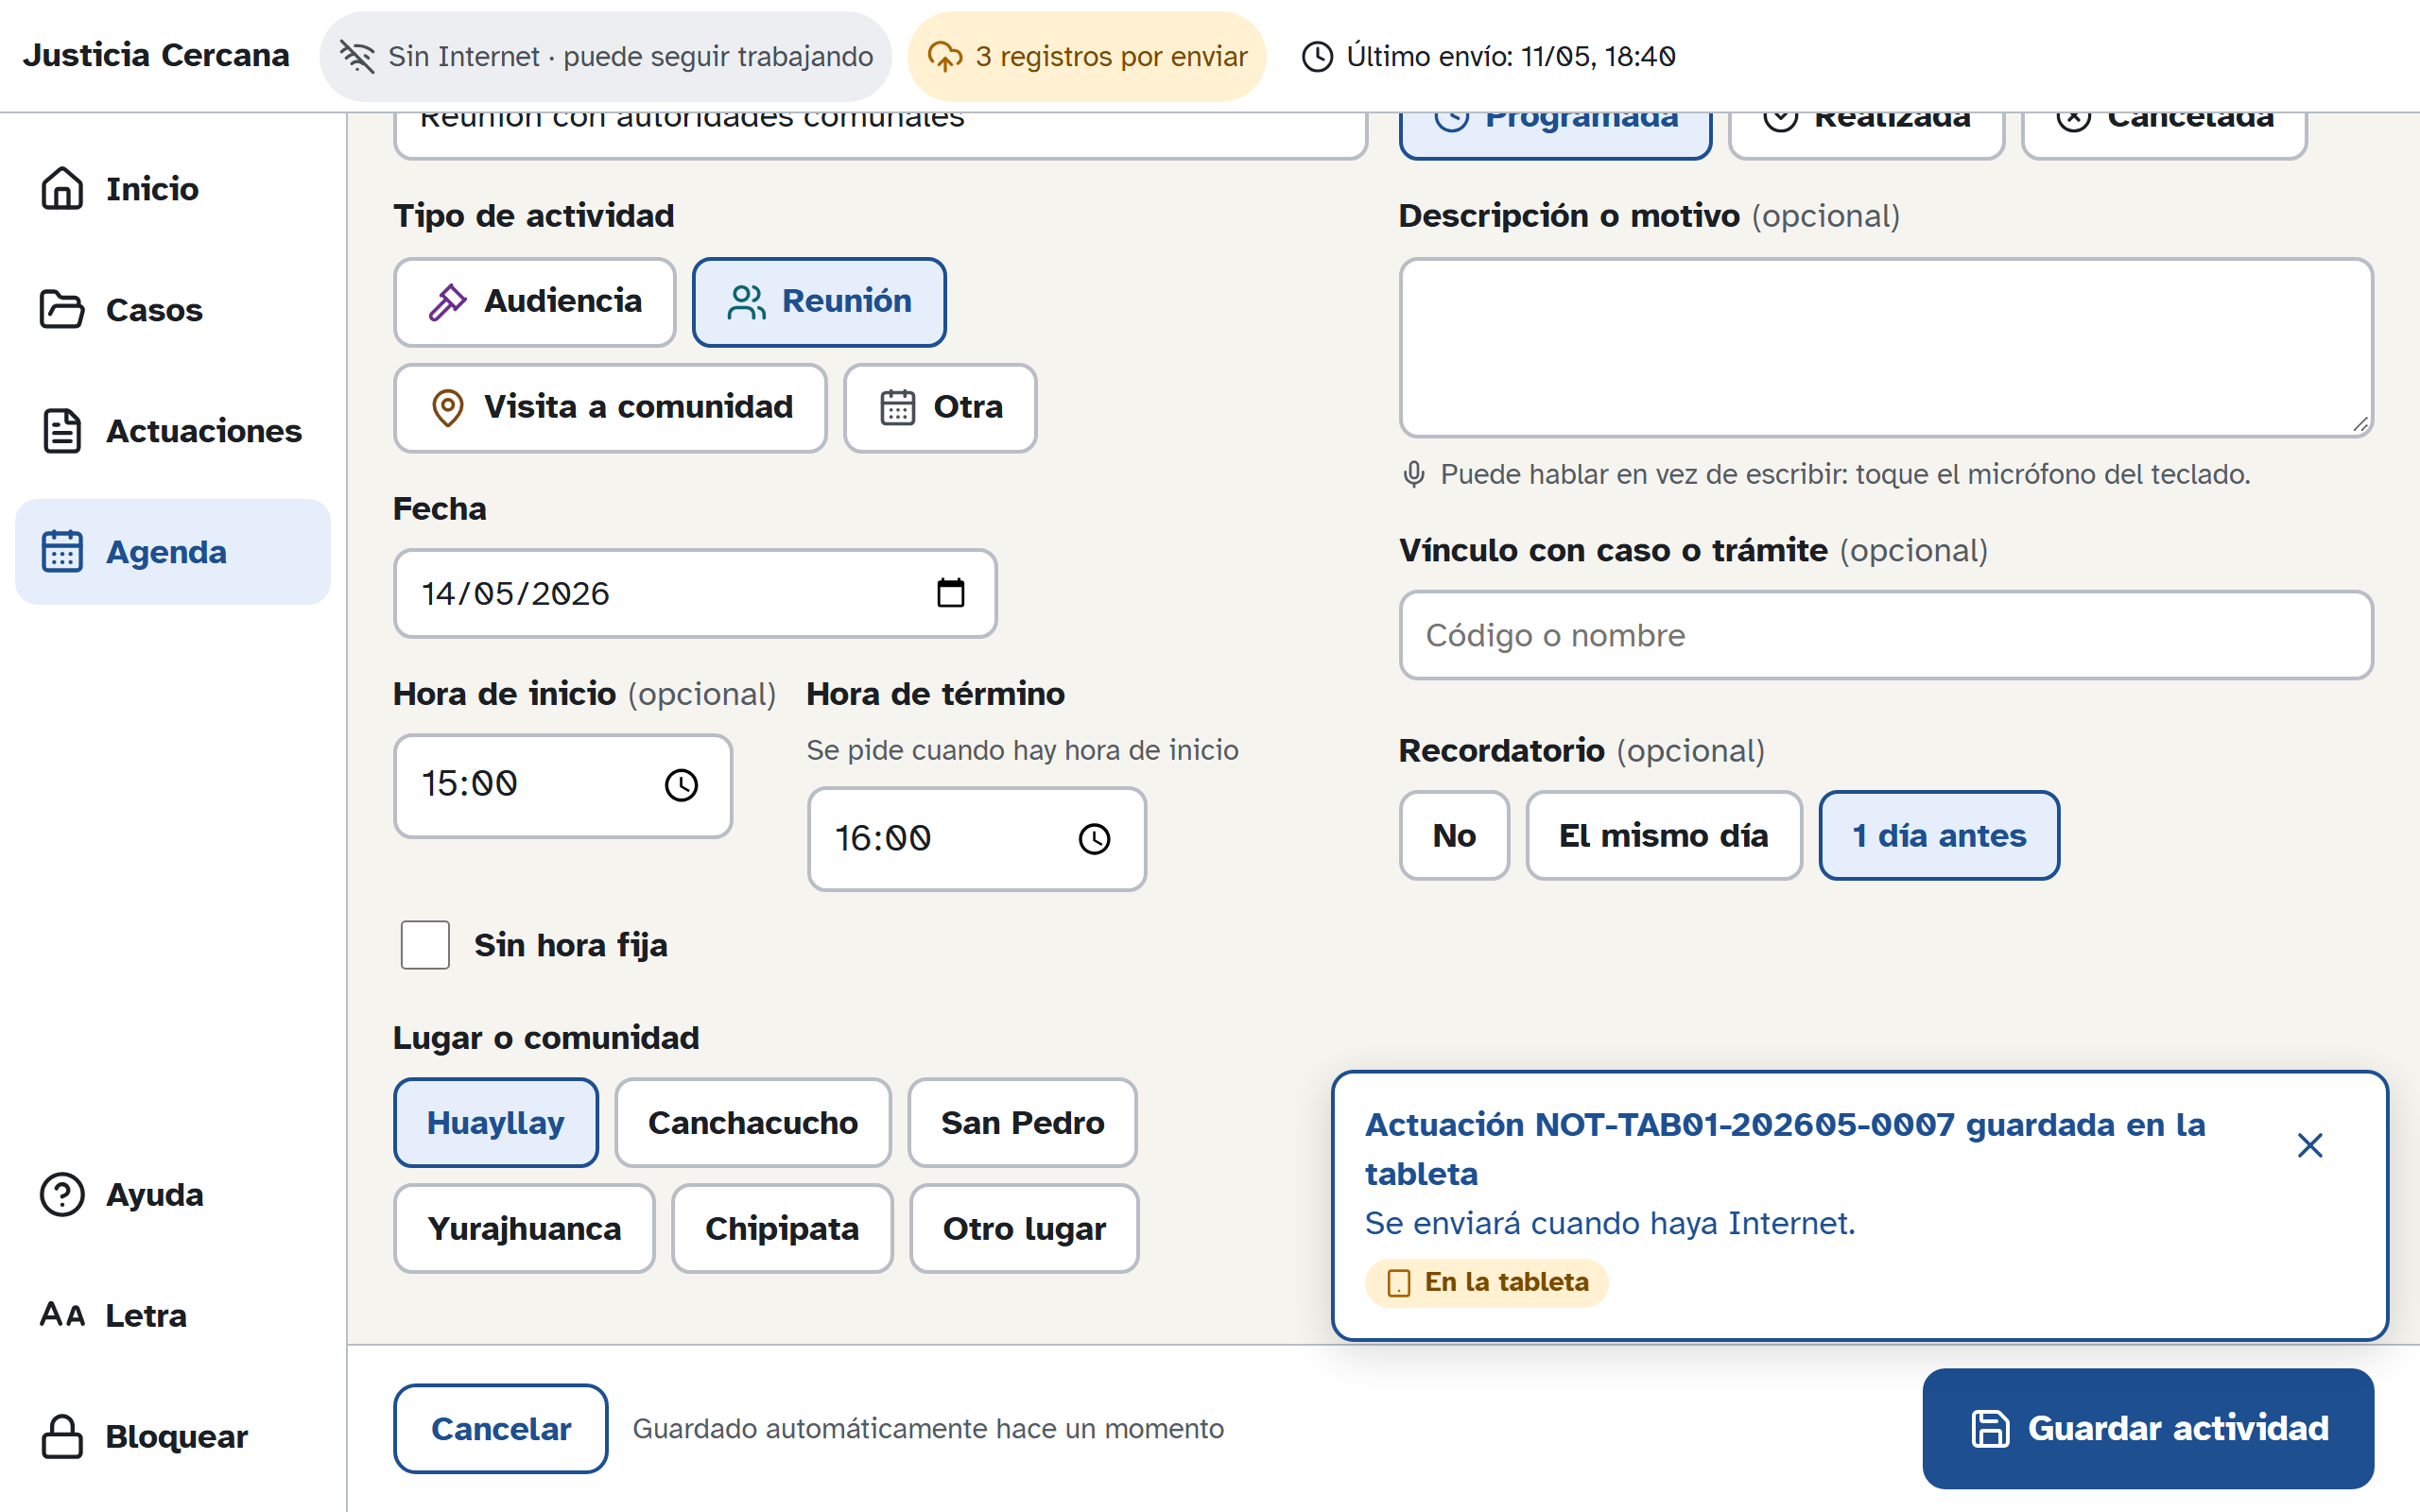
\includegraphics[width=\linewidth]{../../captures/F4-01_nueva-actividad.png}\\[-2pt]{\footnotesize\raggedright\textbf{P-08 · 1.} Reunión con autoridades comunales, jueves 14/05 15:00–16:00, Huayllay \emph{(Cobertura y funcionamiento de los módulos)}\par}\end{minipage}\hfill
\begin{minipage}[t]{0.49\textwidth}\centering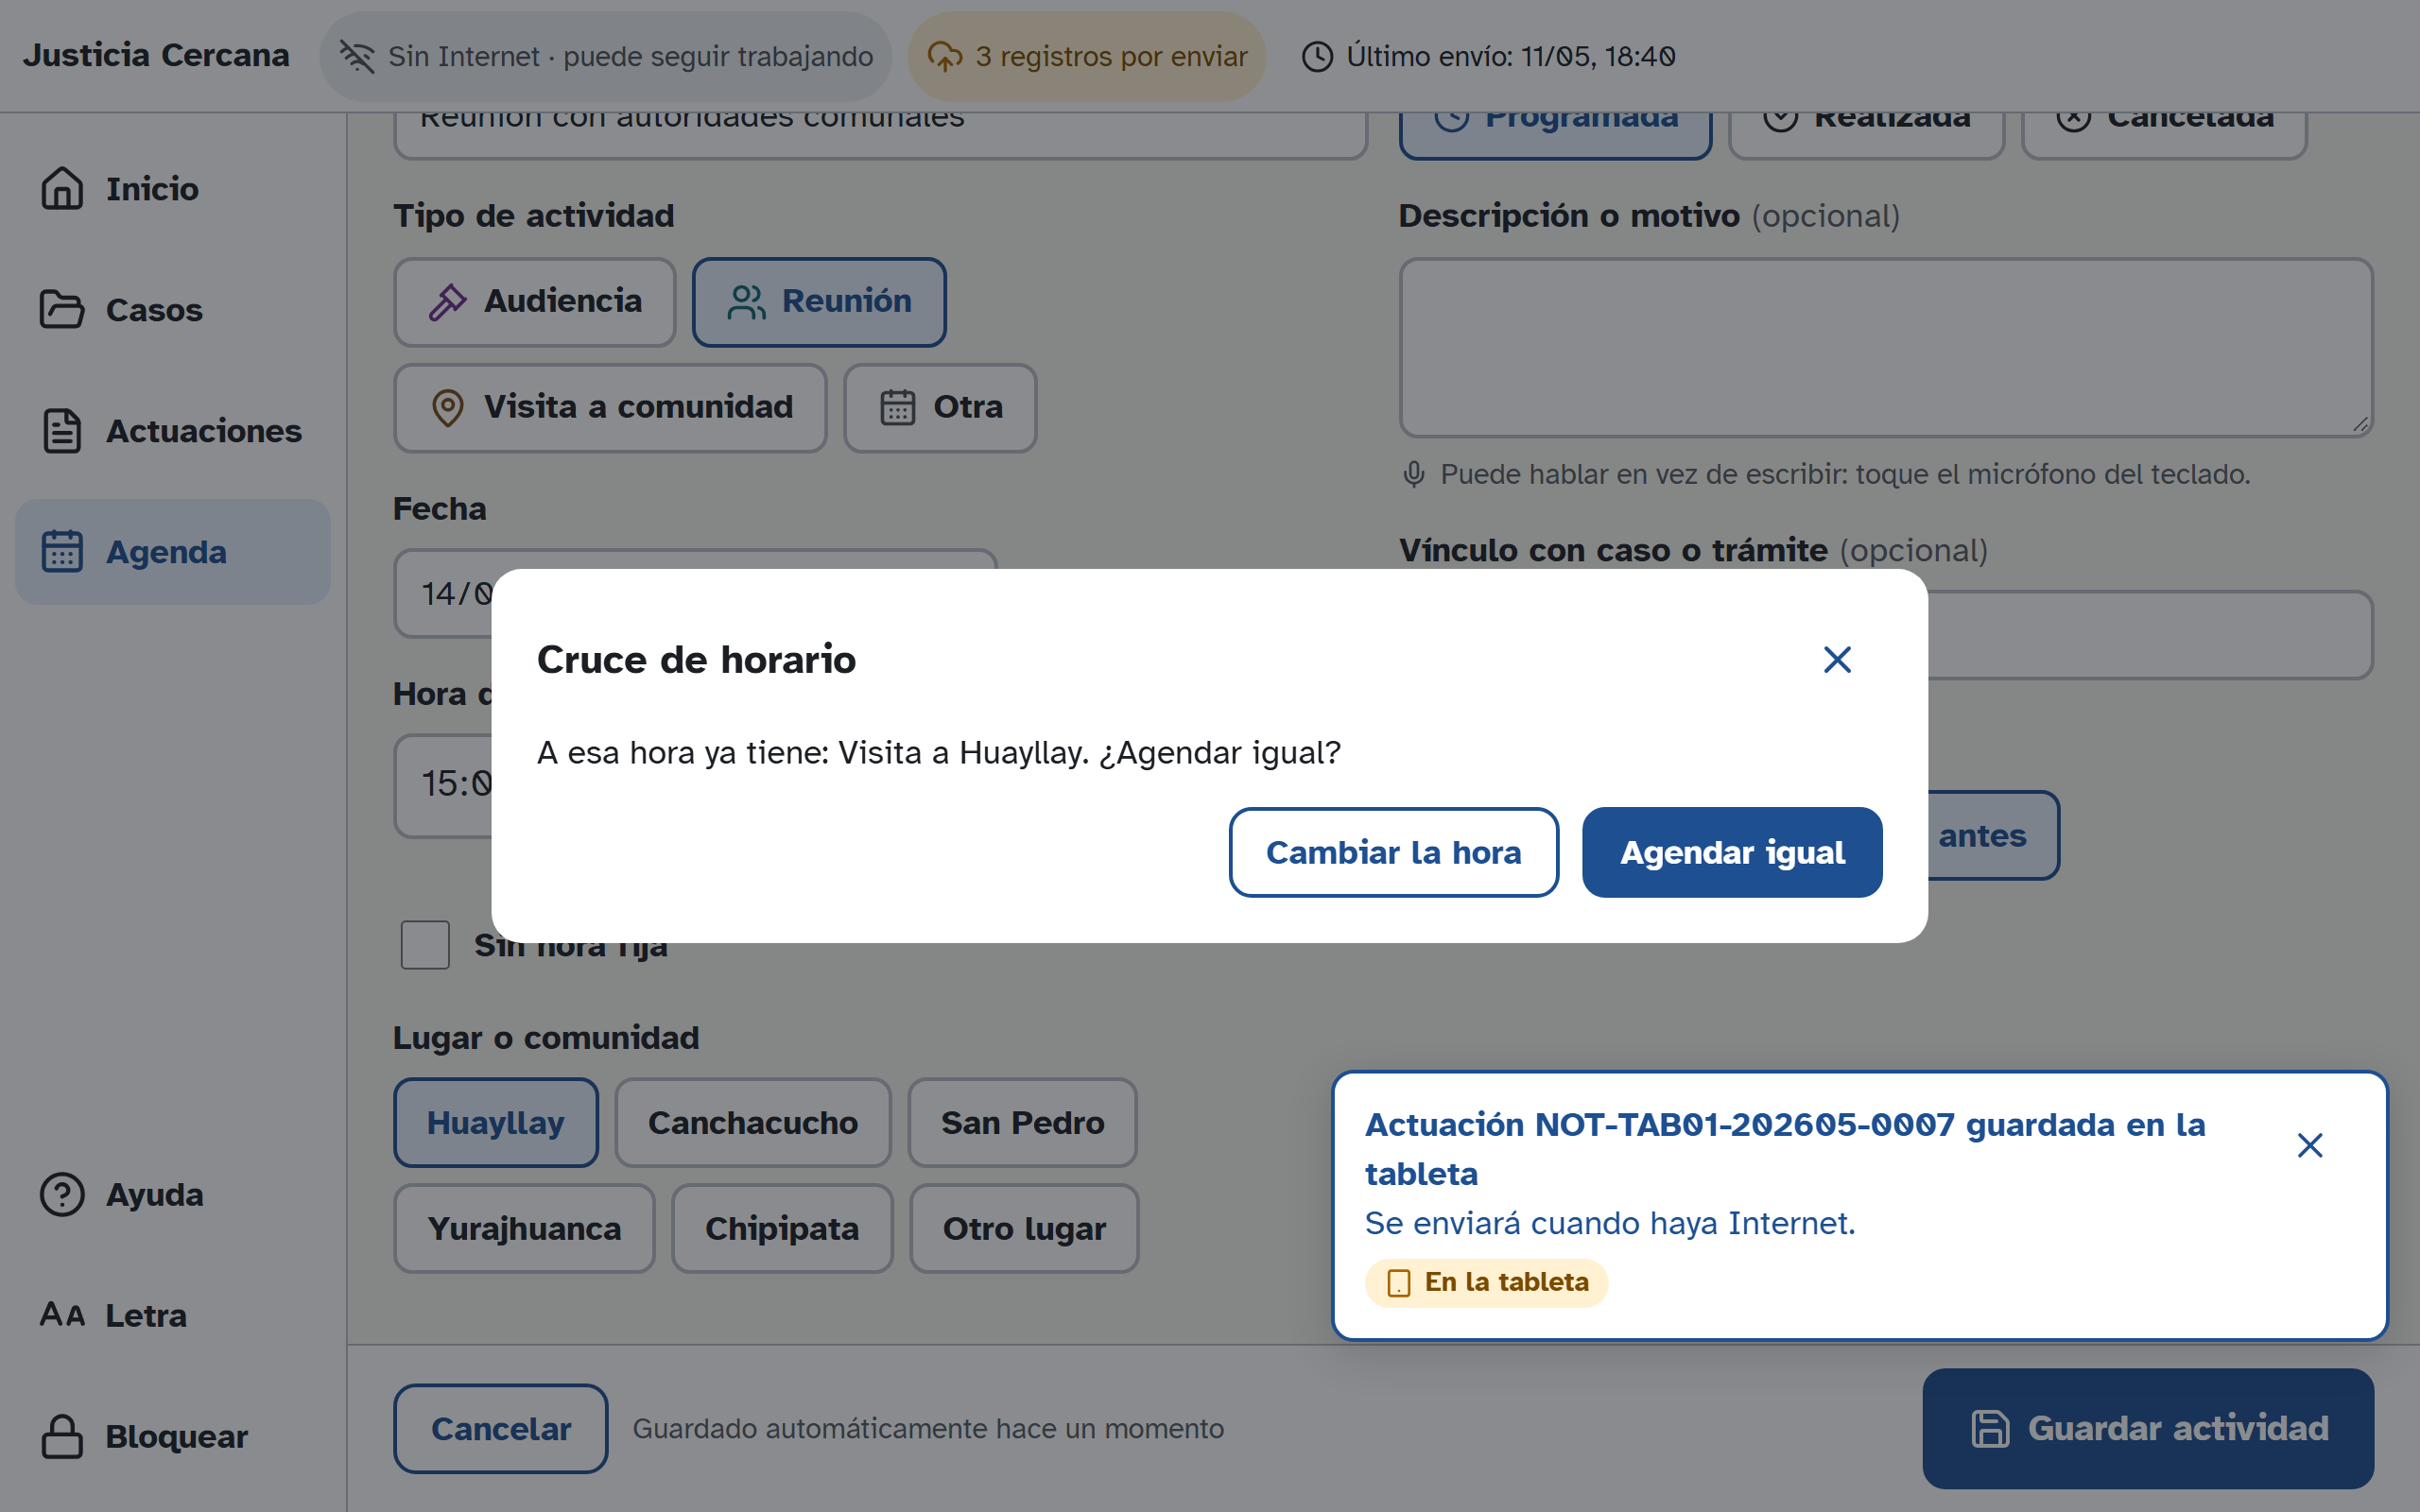
\includegraphics[width=\linewidth]{../../captures/F4-02a_cruce-horario.png}\\[-2pt]{\footnotesize\raggedright\textbf{P-08 · 2.} Aviso no bloqueante de cruce de horario con la otra actividad \emph{(Principios de diseño y heurísticas)}\par}\end{minipage}\par\vspace{8pt}\noindent
\begin{minipage}[t]{0.49\textwidth}\centering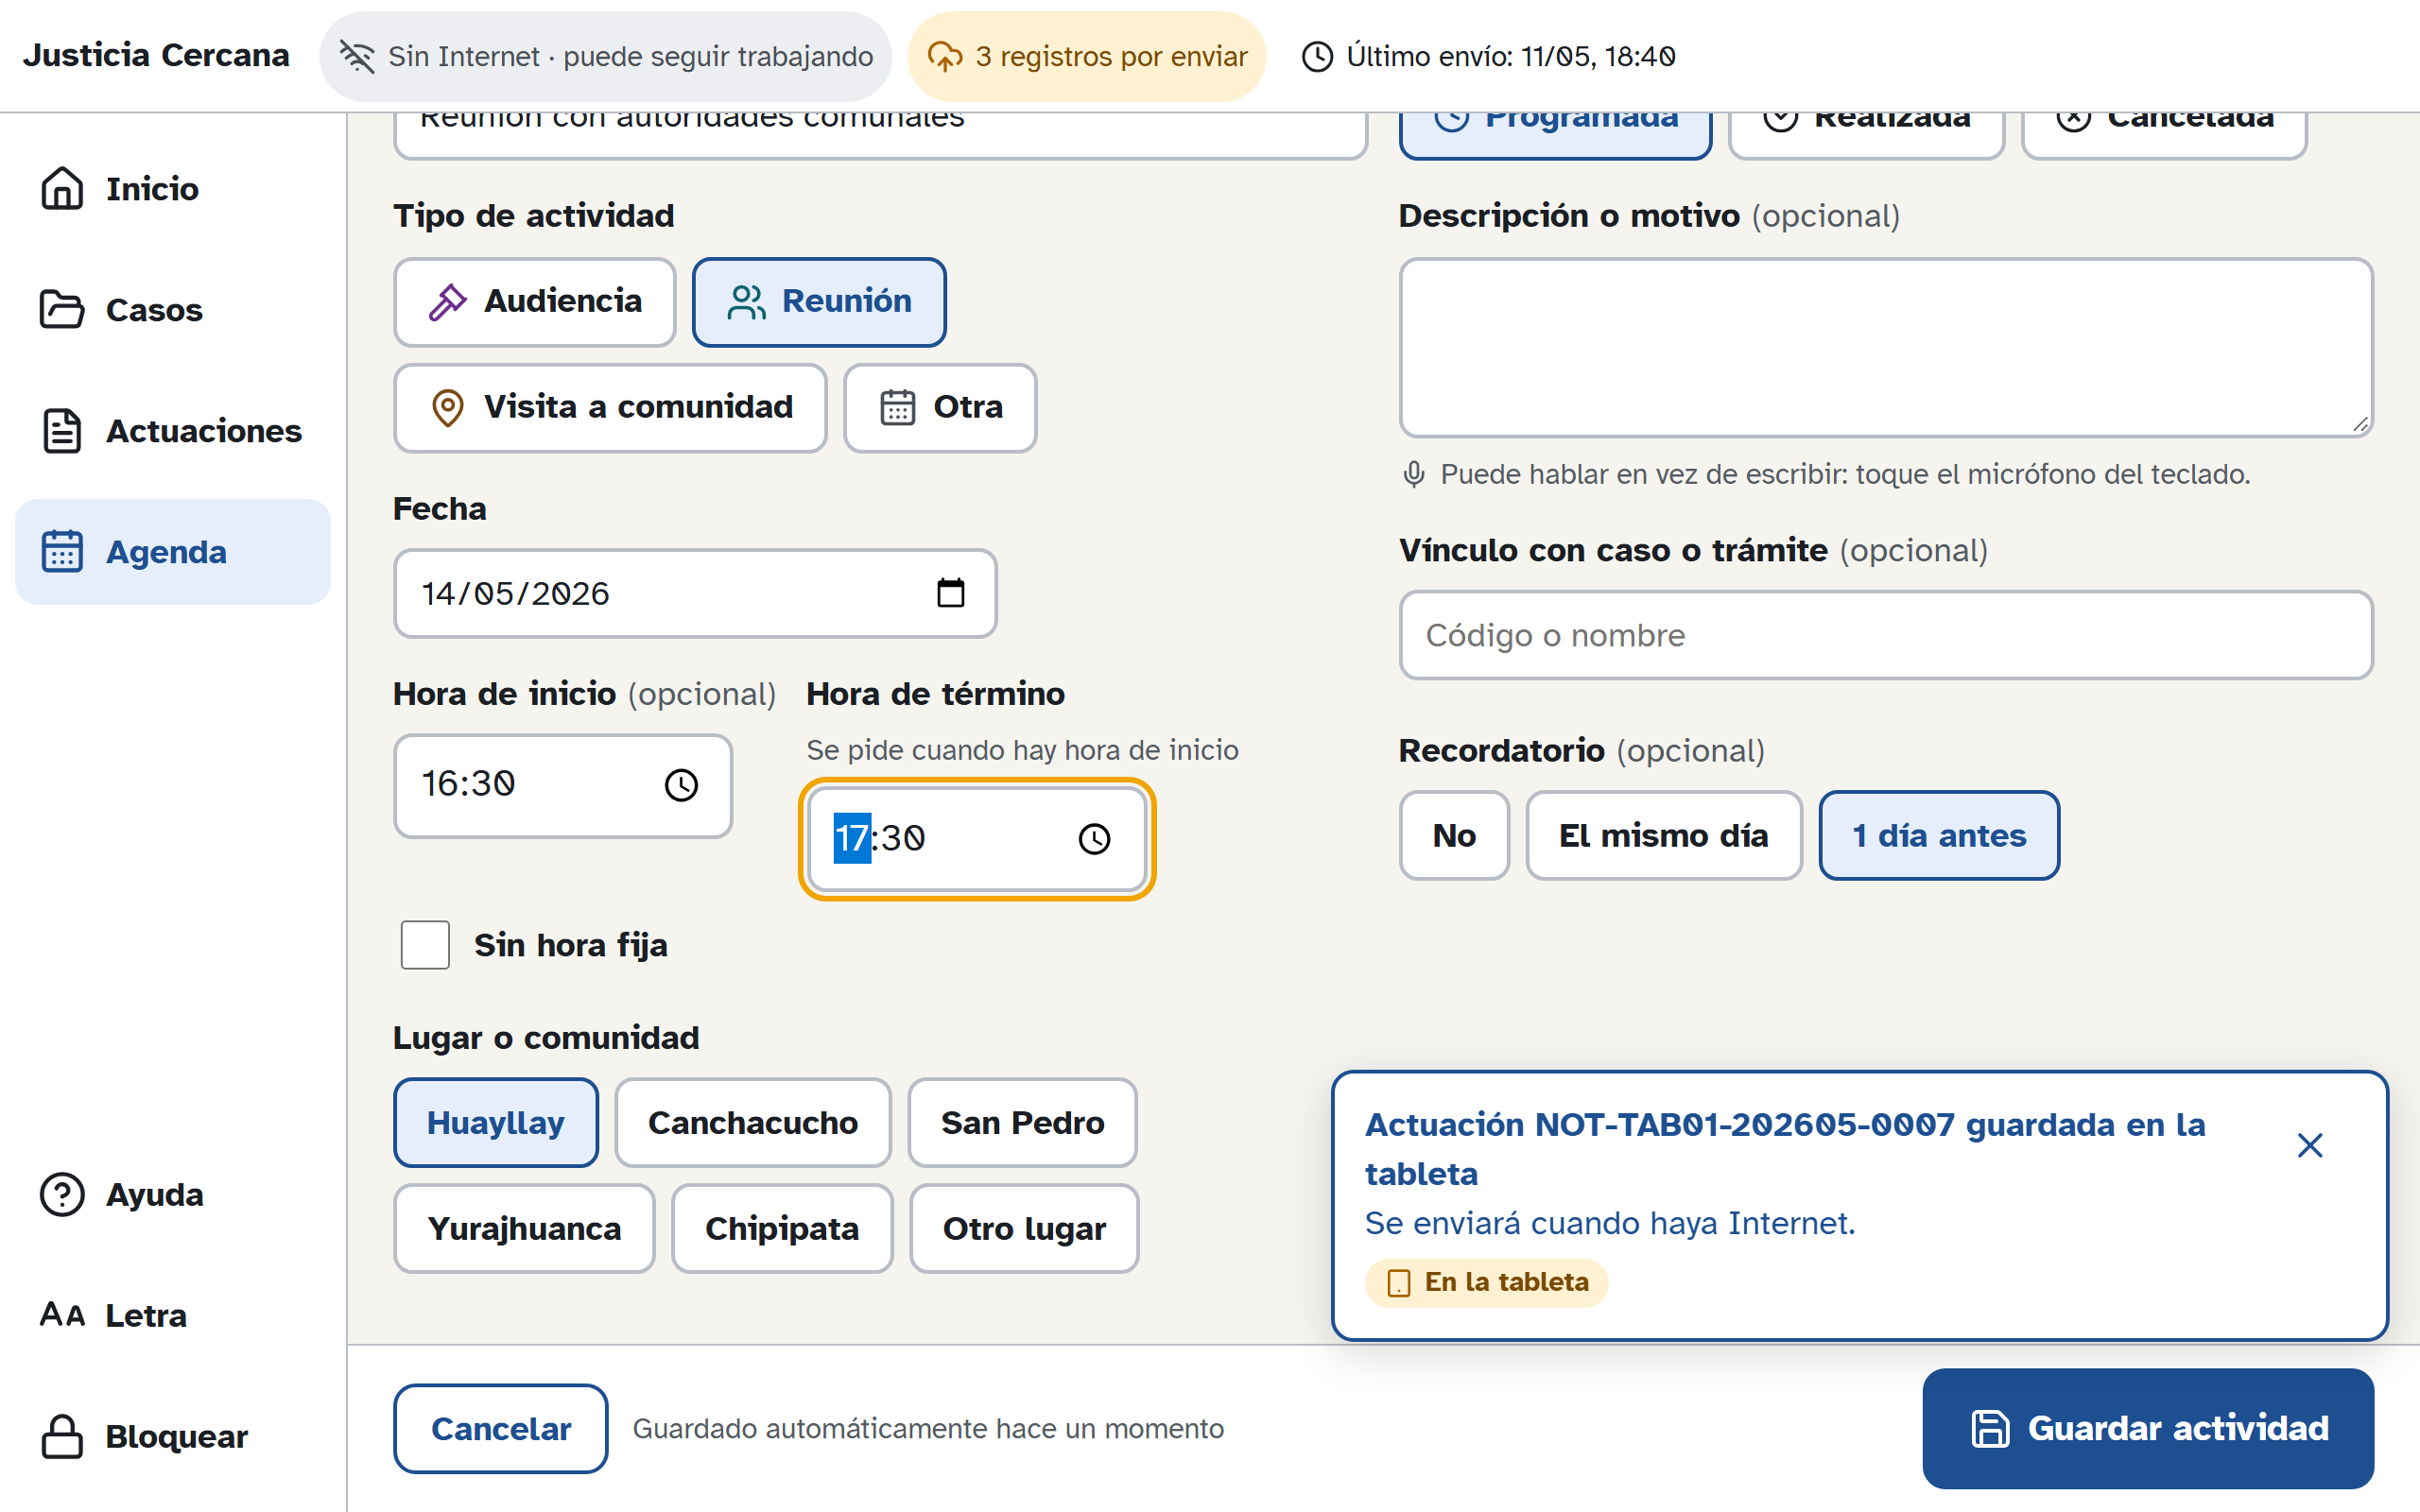
\includegraphics[width=\linewidth]{../../captures/F4-02b_hora-ajustada.png}\\[-2pt]{\footnotesize\raggedright\textbf{P-08 · 2.} Hora ajustada a 16:30–17:30 \emph{(Cobertura y funcionamiento de los módulos)}\par}\end{minipage}\hfill
\begin{minipage}[t]{0.49\textwidth}\centering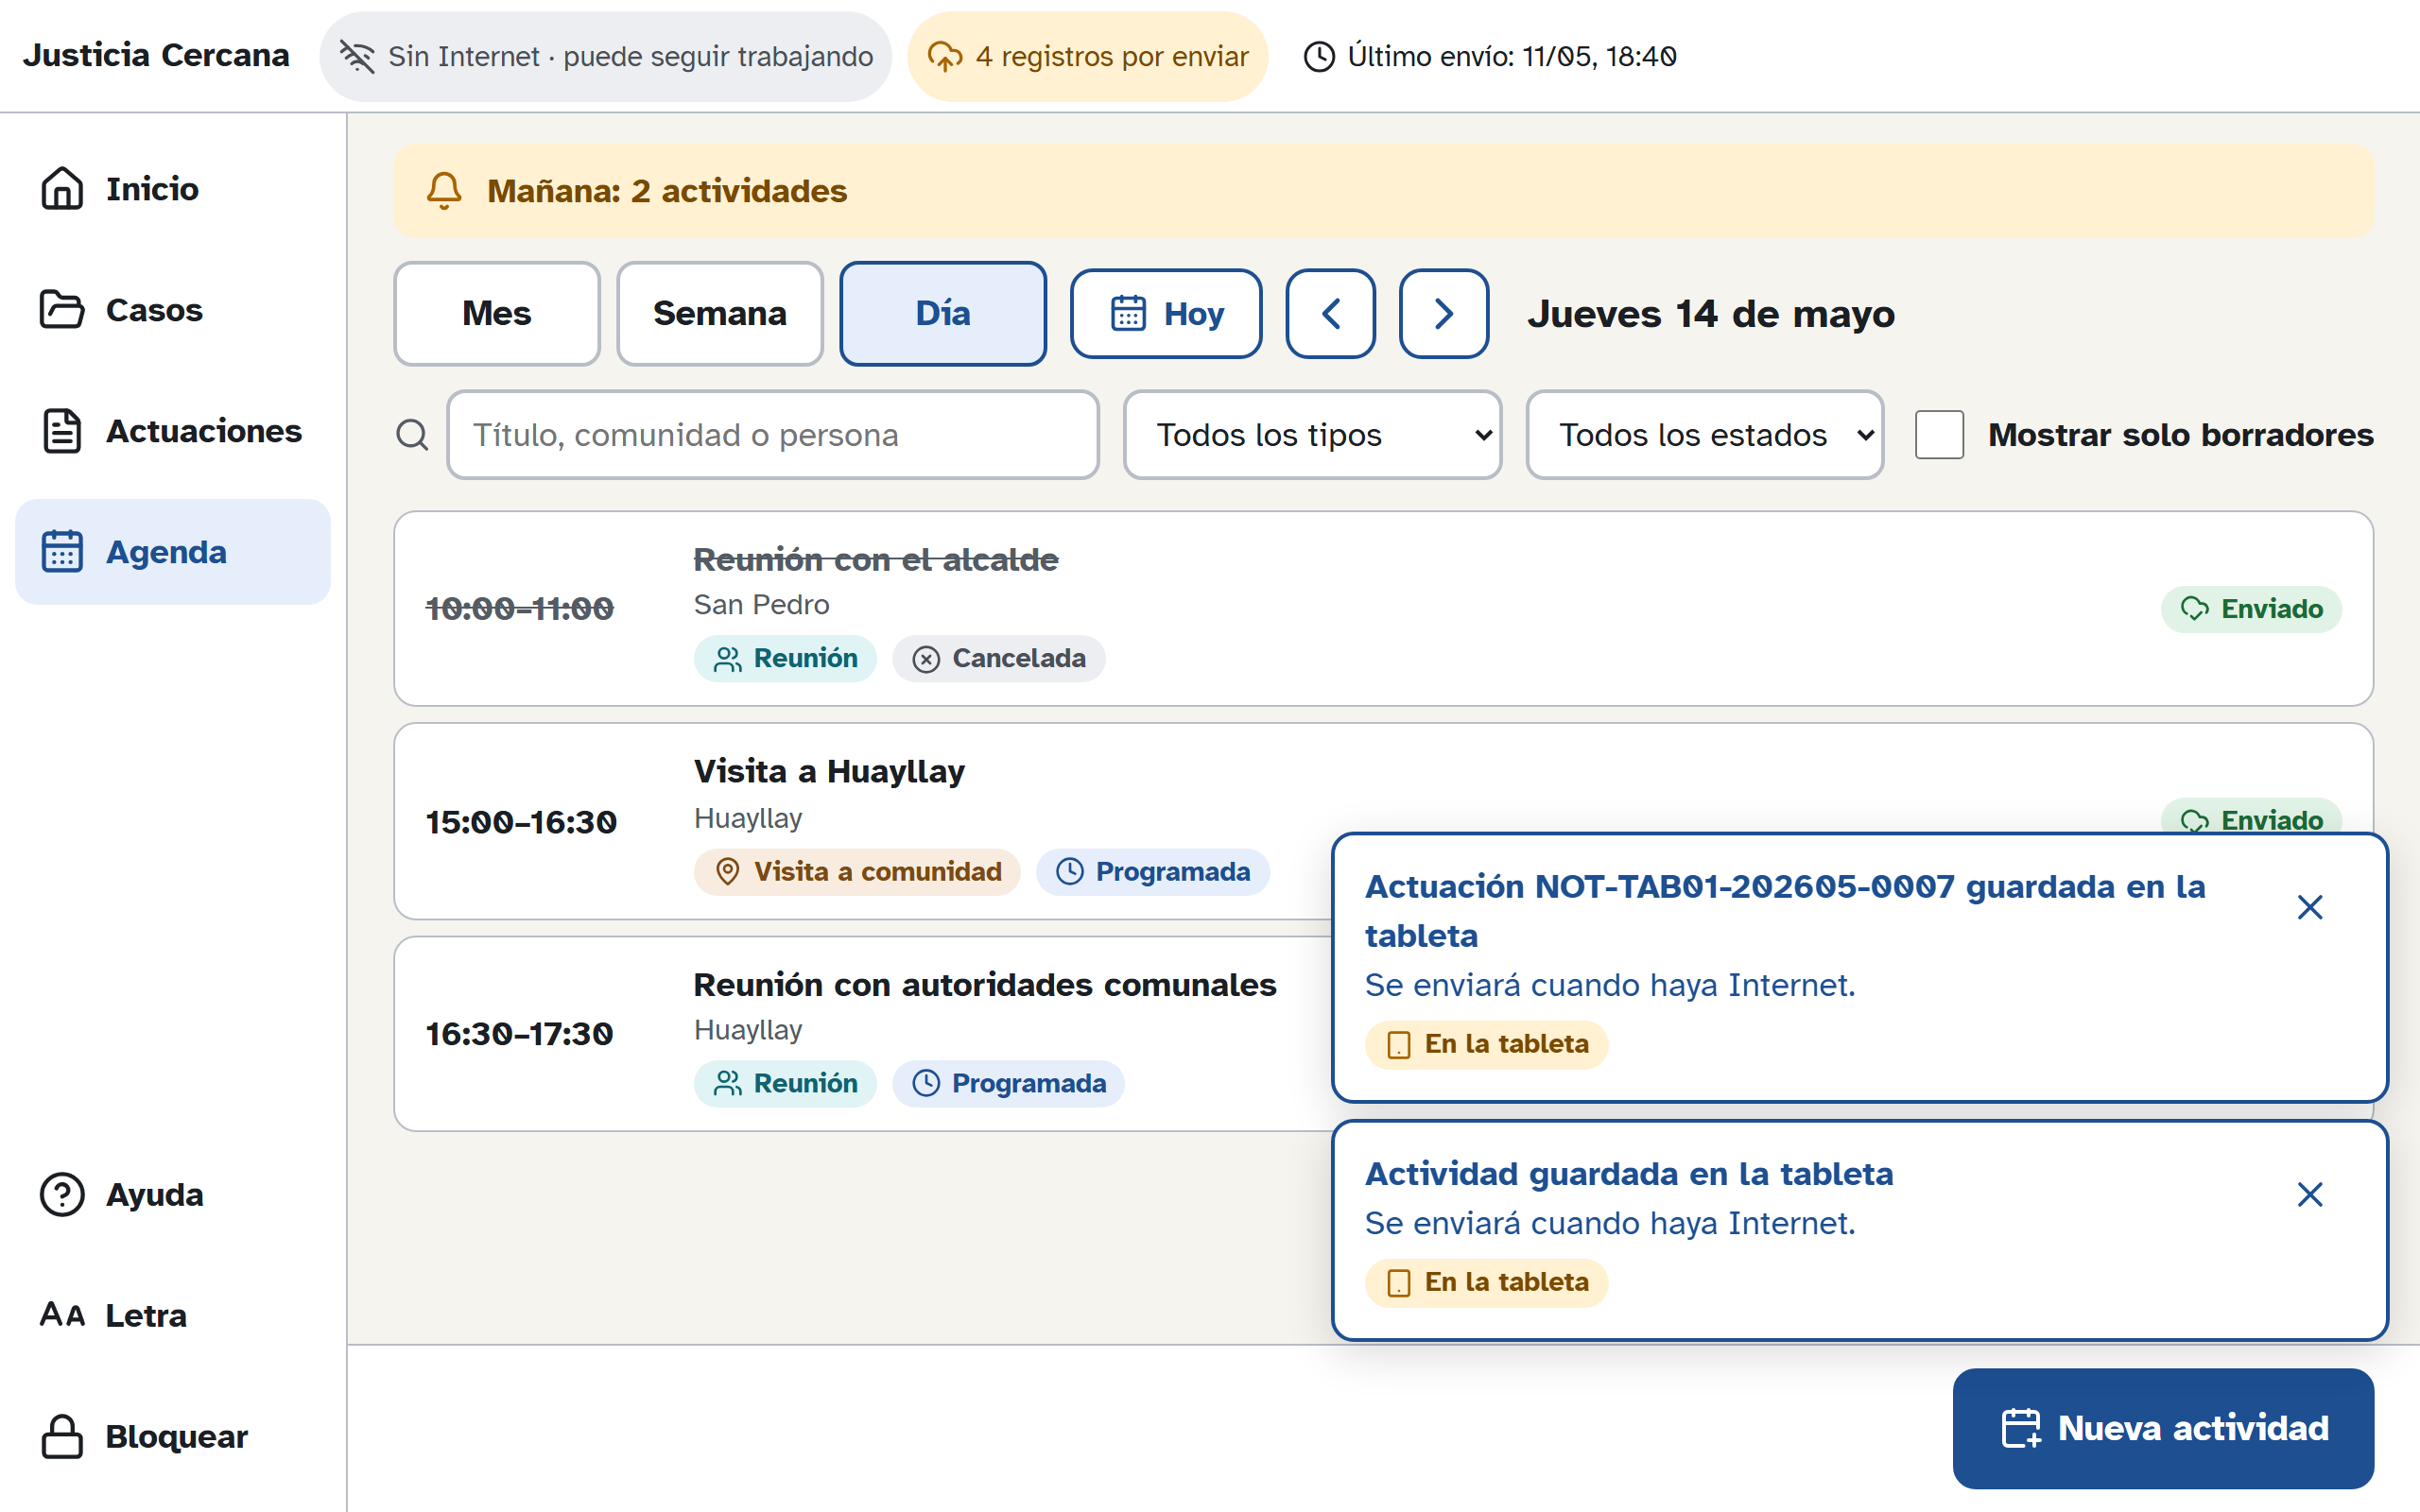
\includegraphics[width=\linewidth]{../../captures/F4-03_guardado-por-enviar.png}\\[-2pt]{\footnotesize\raggedright\textbf{P-07 · 3.} Guardada; barra ``4 registros por enviar'' \emph{(Funcionamiento sin conexión)}\par}\end{minipage}\par\vspace{8pt}\noindent
\begin{minipage}[t]{0.49\textwidth}\centering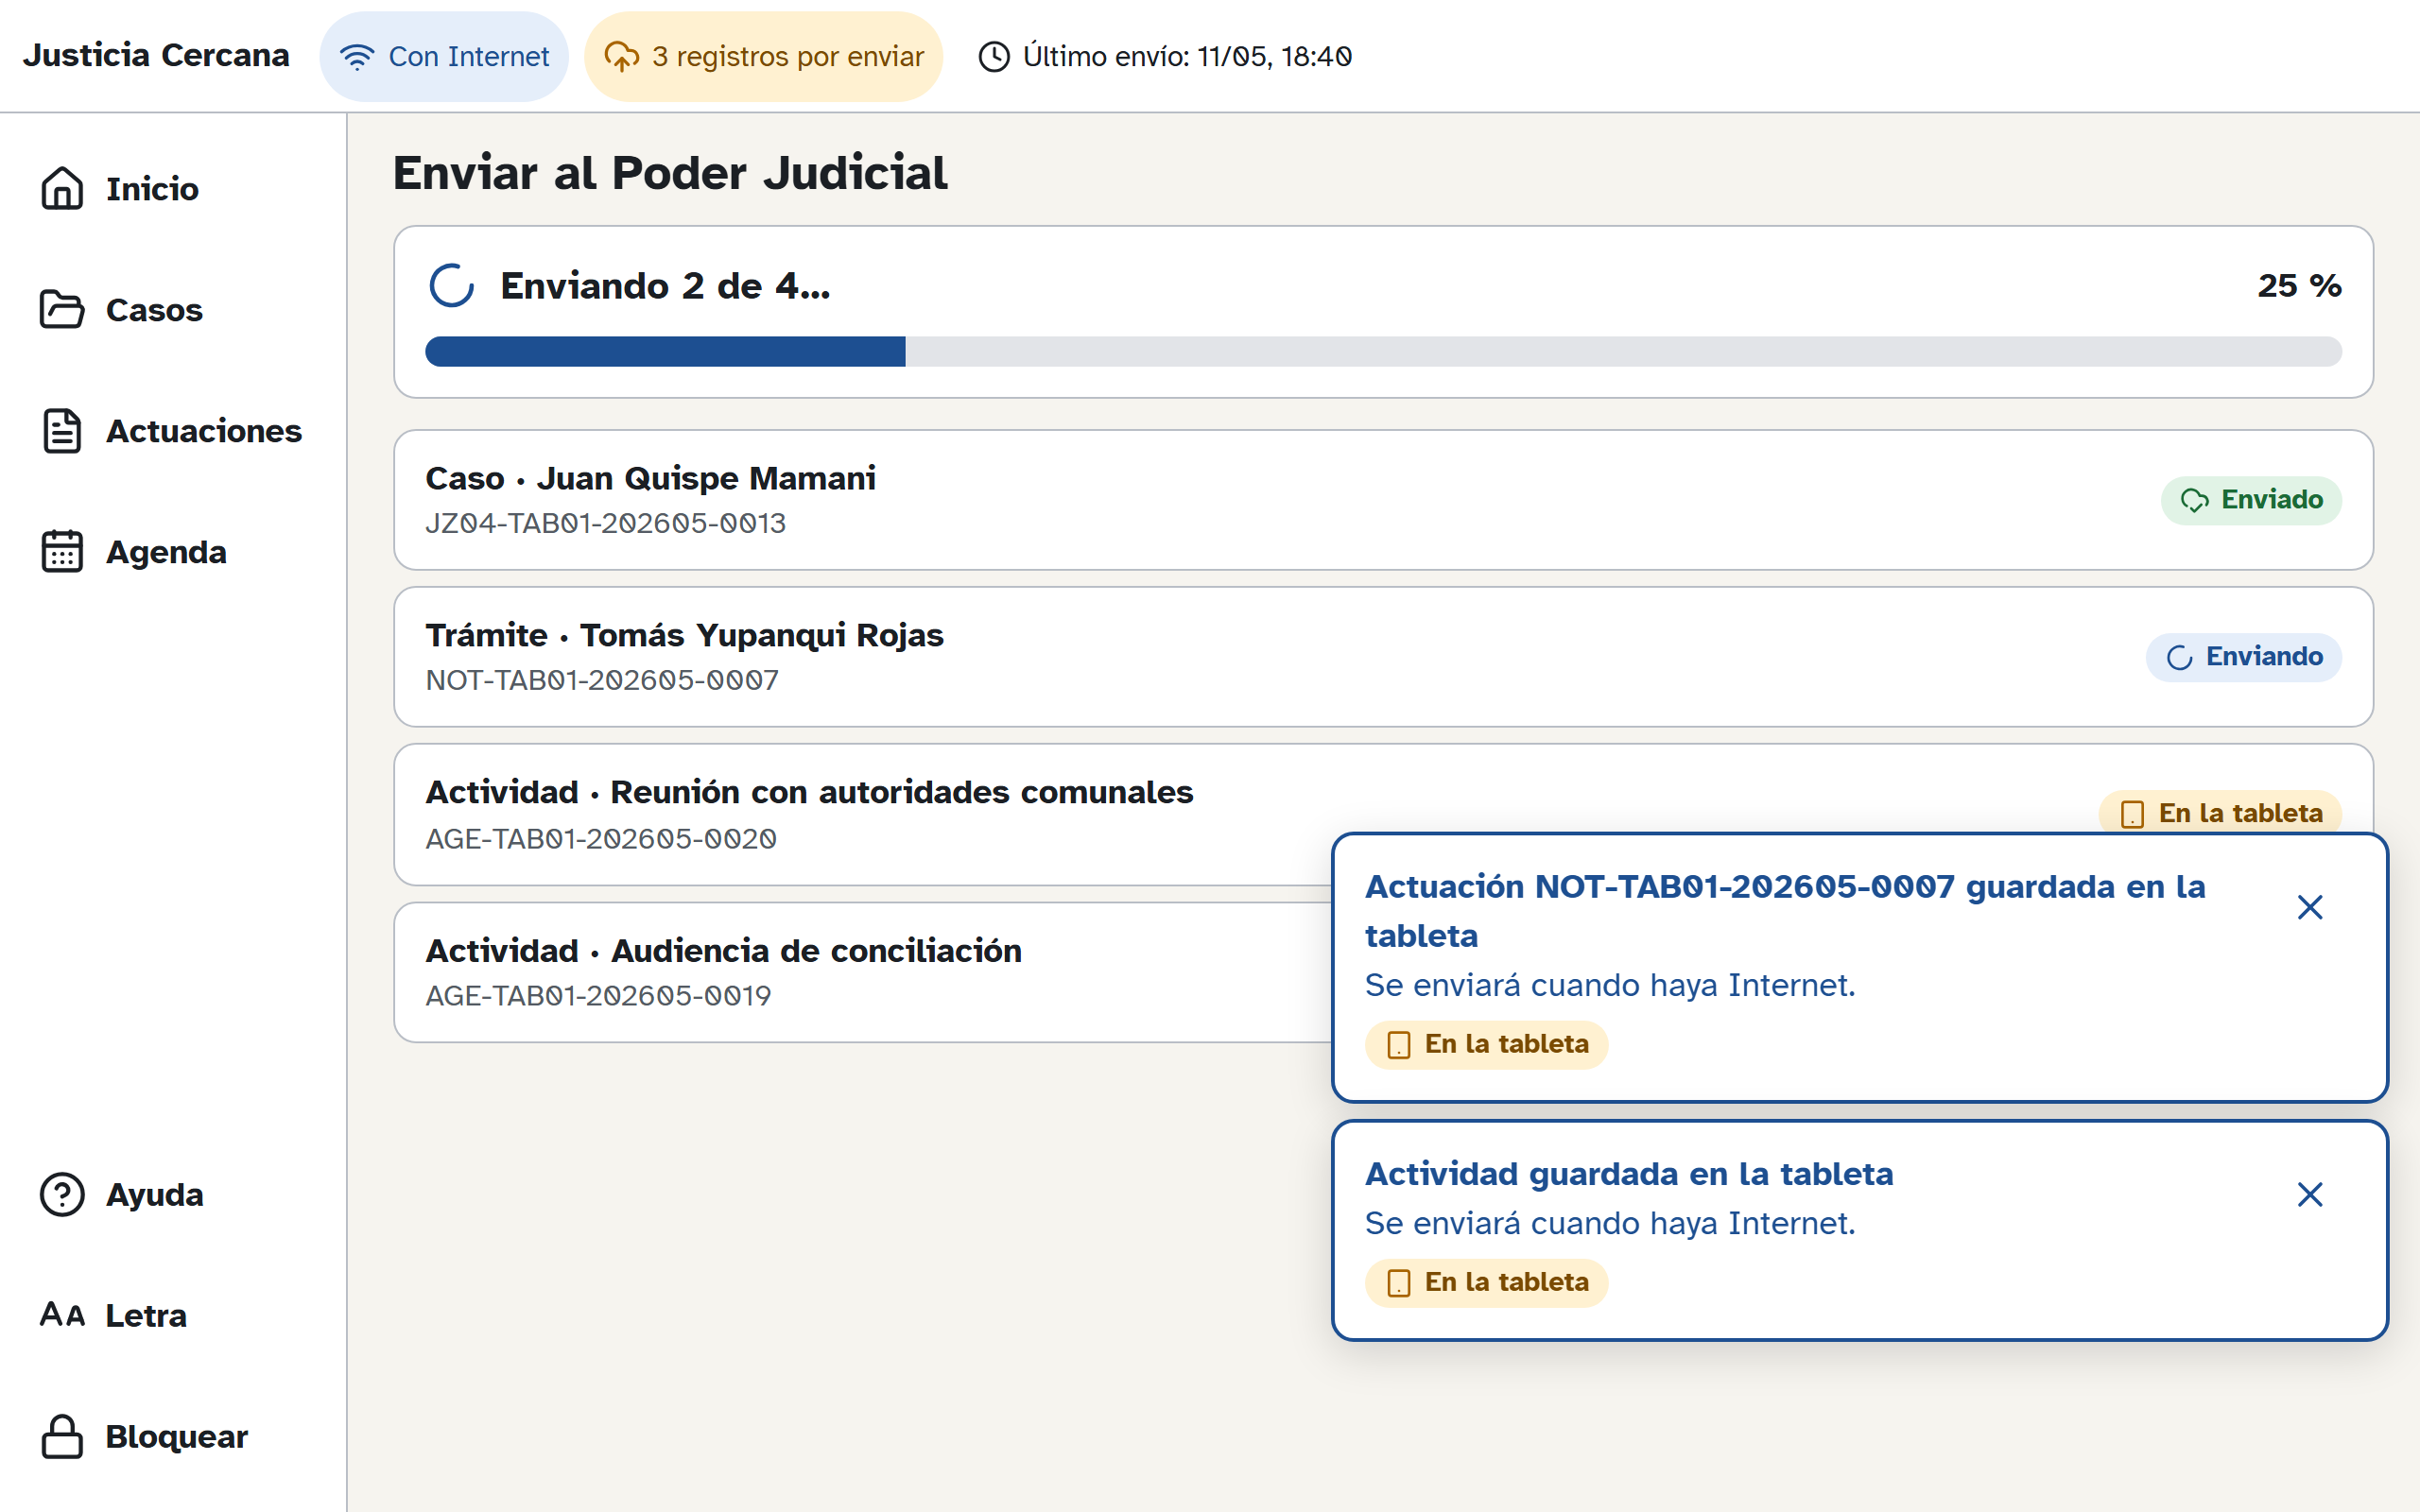
\includegraphics[width=\linewidth]{../../captures/F4-04_progreso-envio.png}\\[-2pt]{\footnotesize\raggedright\textbf{P-09 · 4.} Envío automático al volver el Internet con progreso ``Enviando n de 4…'' \emph{(Funcionamiento sin conexión)}\par}\end{minipage}\hfill
\begin{minipage}[t]{0.49\textwidth}\centering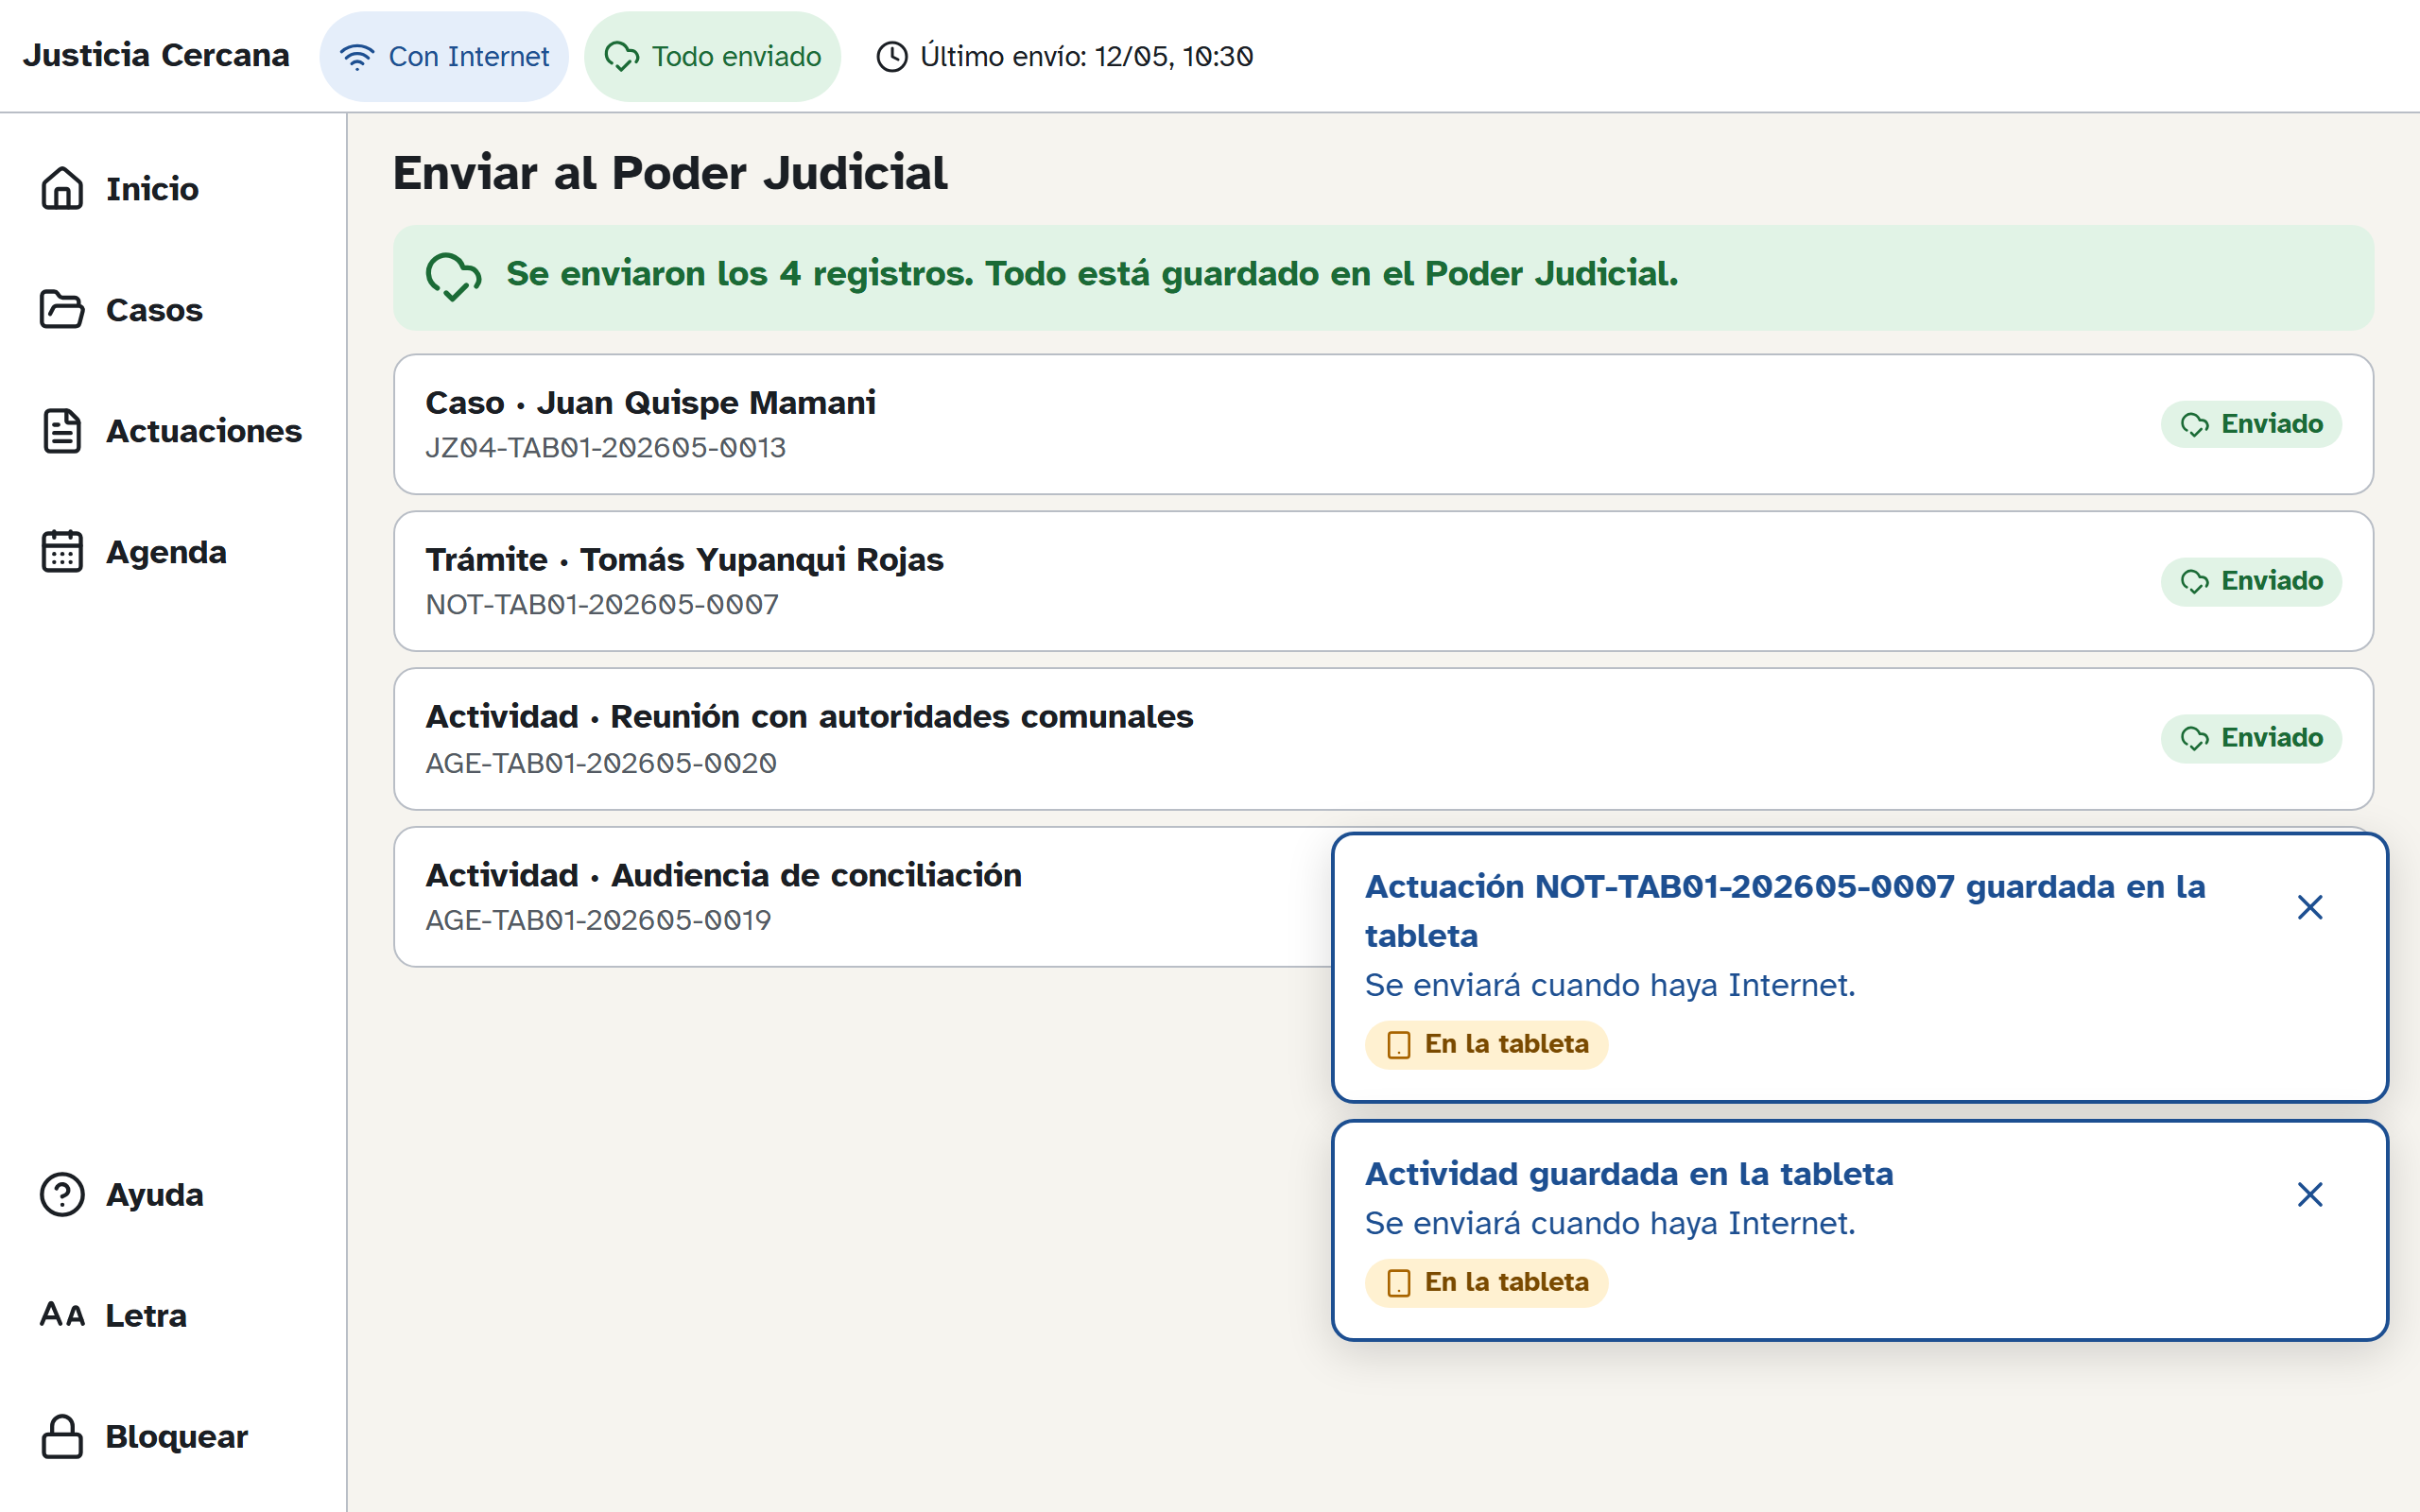
\includegraphics[width=\linewidth]{../../captures/F4-05a_exito-todo-enviado.png}\\[-2pt]{\footnotesize\raggedright\textbf{P-09 · 5.} ``Se enviaron los 4 registros'' y barra ``Todo enviado''; distintivos ``Enviado'' \emph{(Funcionamiento sin conexión)}\par}\end{minipage}\par\vspace{8pt}\noindent
\begin{minipage}[t]{0.49\textwidth}\centering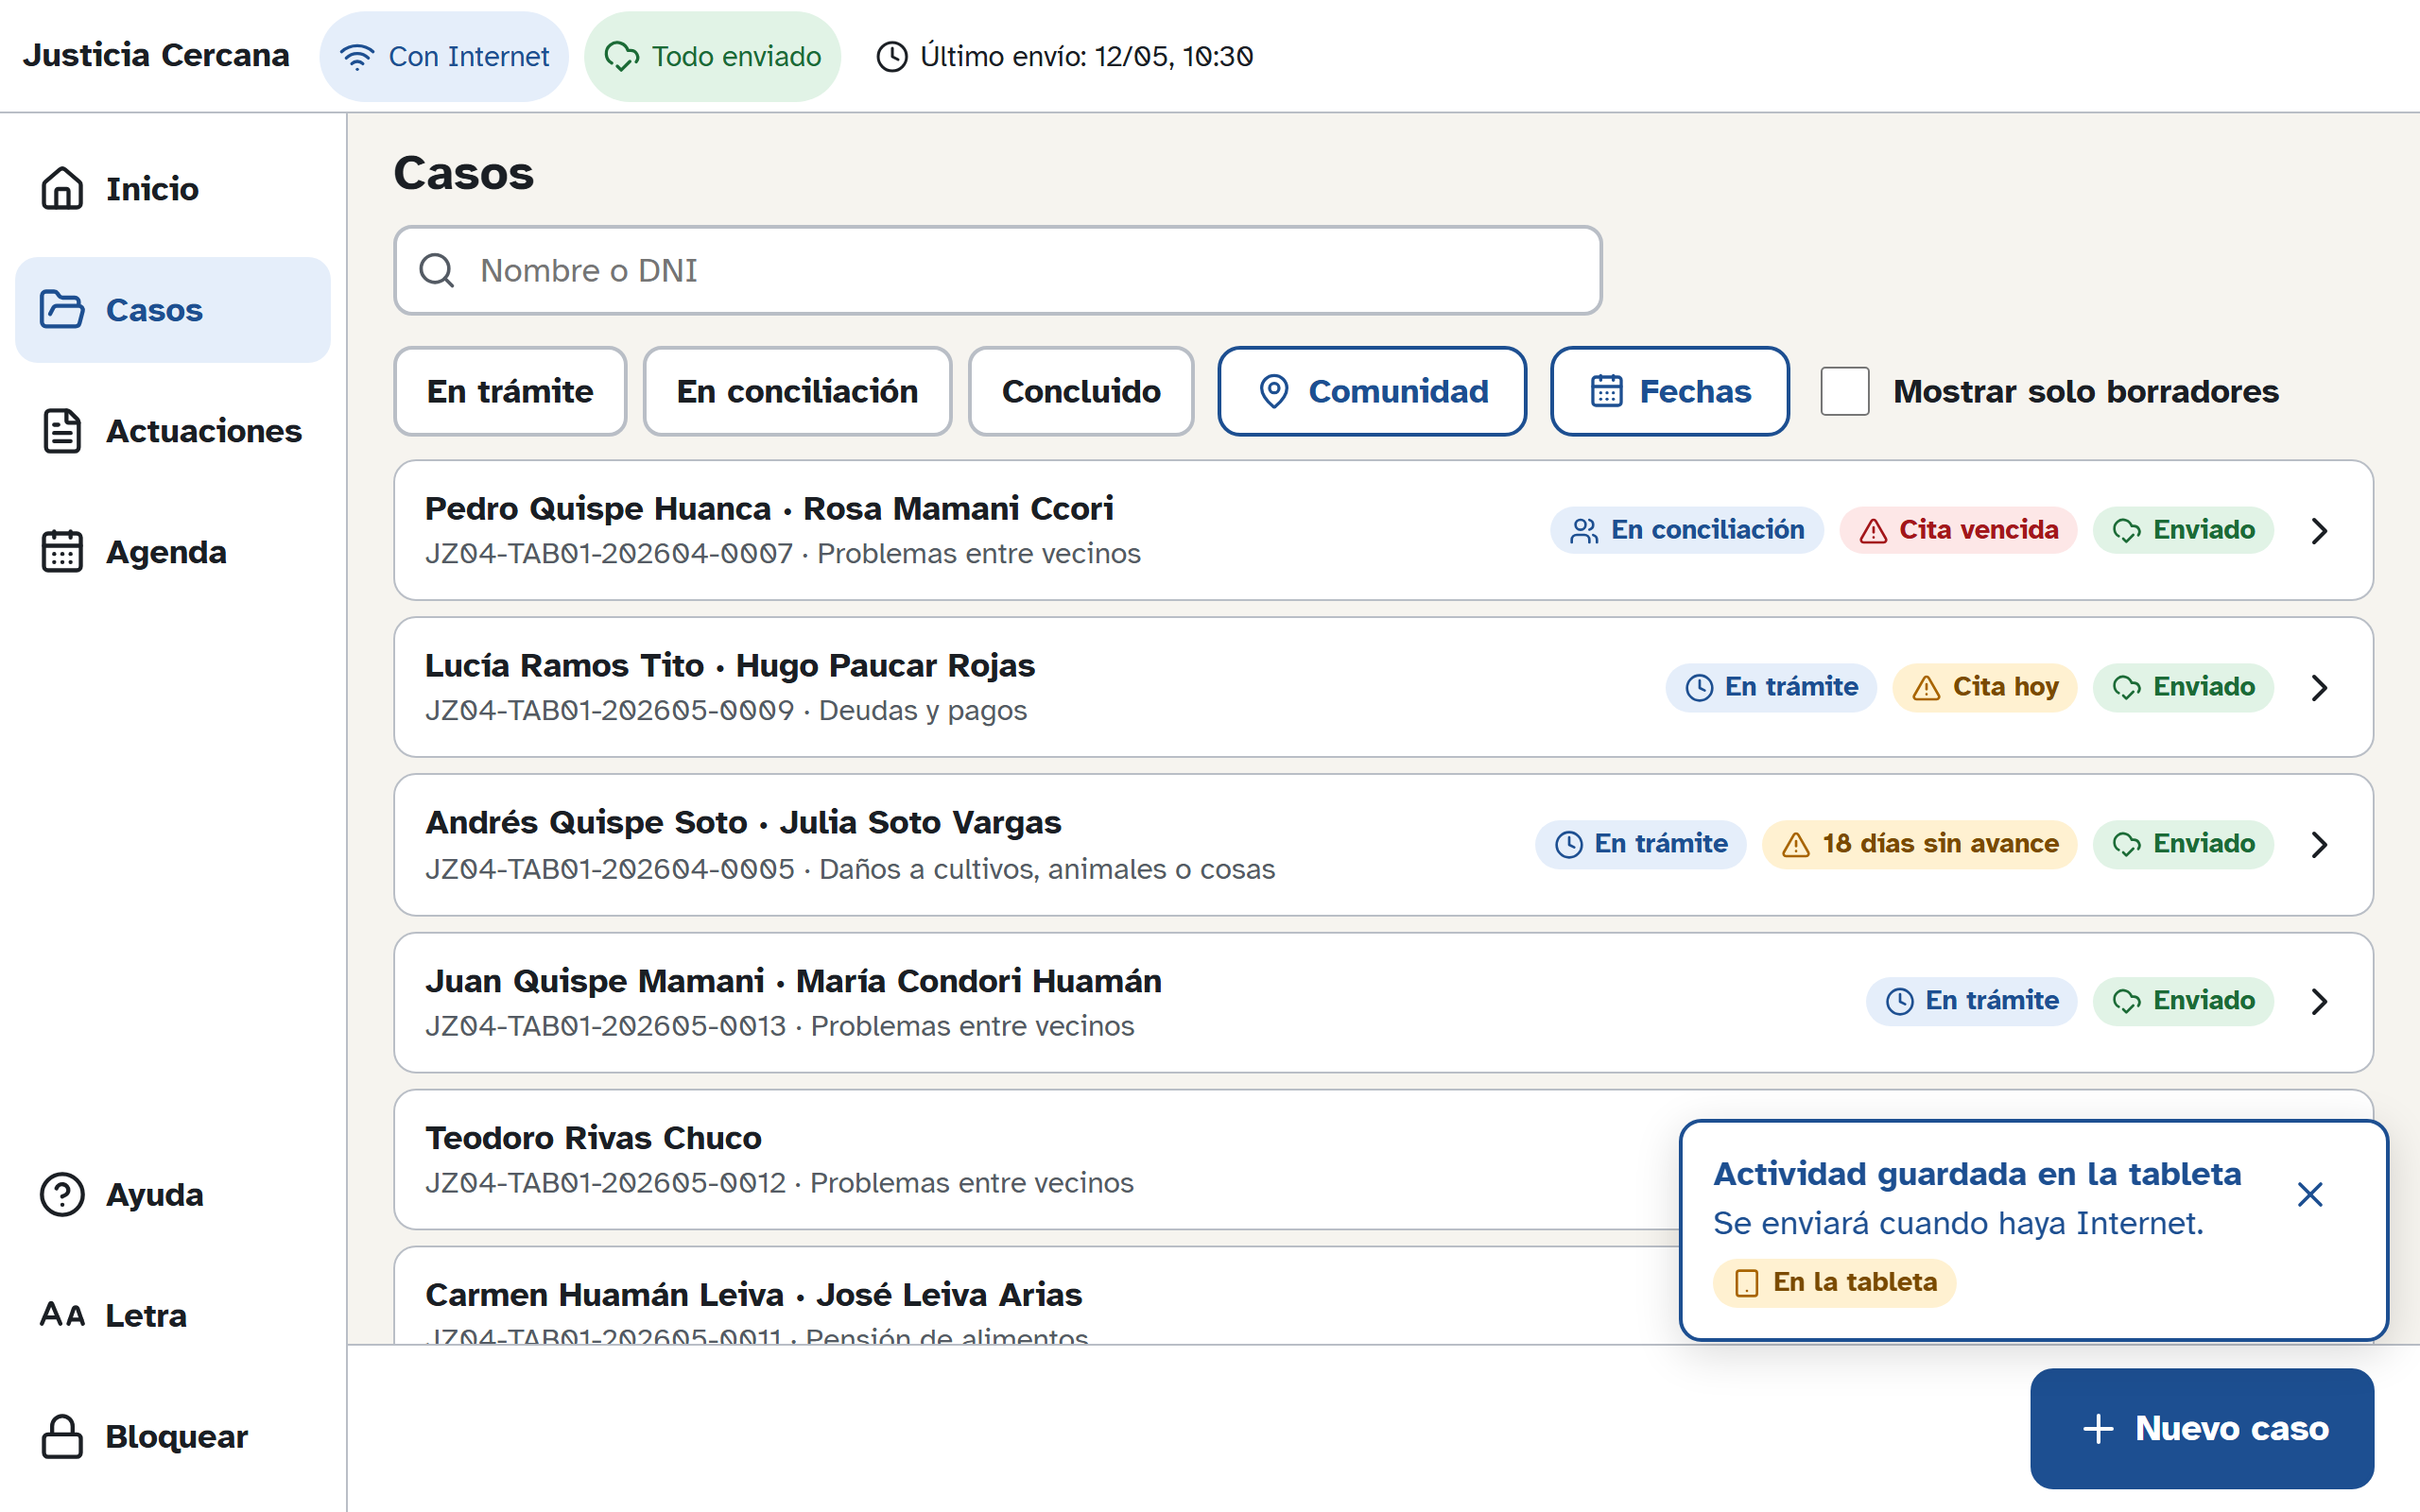
\includegraphics[width=\linewidth]{../../captures/F4-05b_distintivos-enviado.png}\\[-2pt]{\footnotesize\raggedright\textbf{P-02 · 5.} El caso del Flujo 1 pasa a ``Enviado'' en la lista \emph{(Funcionamiento sin conexión)}\par}\end{minipage}\hfill
\begin{minipage}[t]{0.49\textwidth}\centering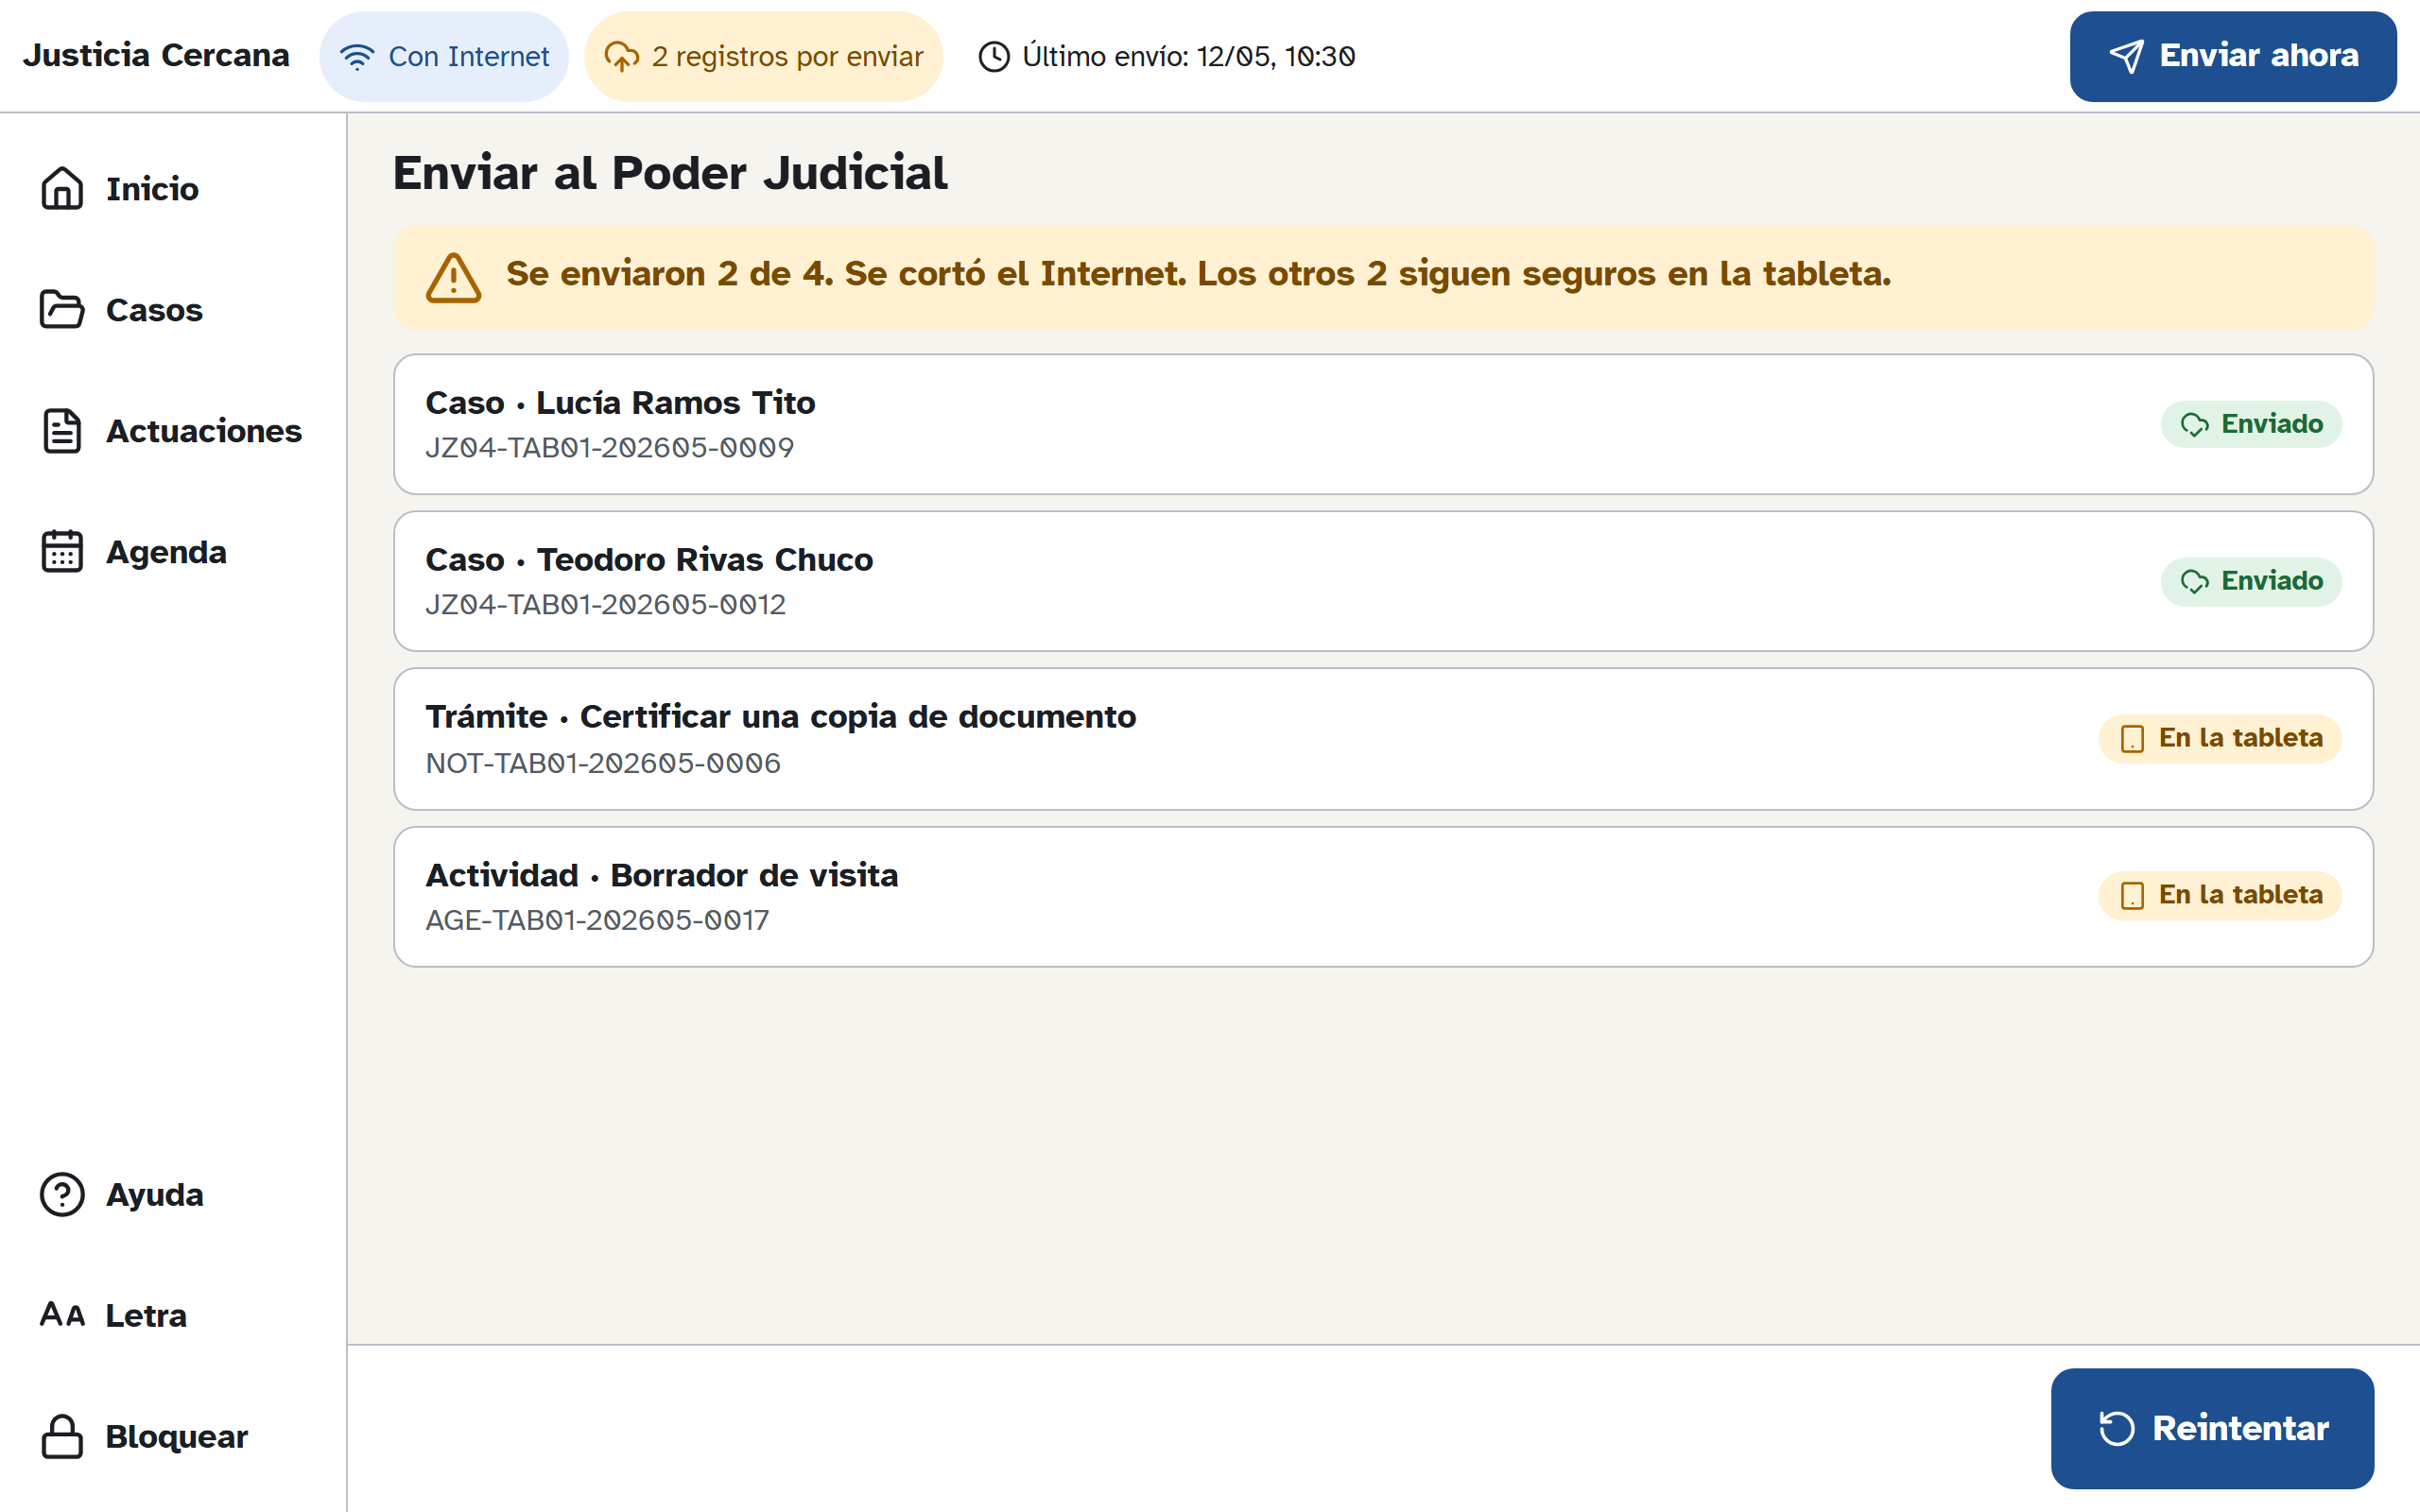
\includegraphics[width=\linewidth]{../../captures/F4-06a_fallo-parcial.png}\\[-2pt]{\footnotesize\raggedright\textbf{P-09 · 6.} Fallo parcial: ``Se enviaron 2 de 4…'' con [Reintentar] \emph{(Funcionamiento sin conexión)}\par}\end{minipage}\par\vspace{8pt}\noindent
\begin{minipage}[t]{0.49\textwidth}\centering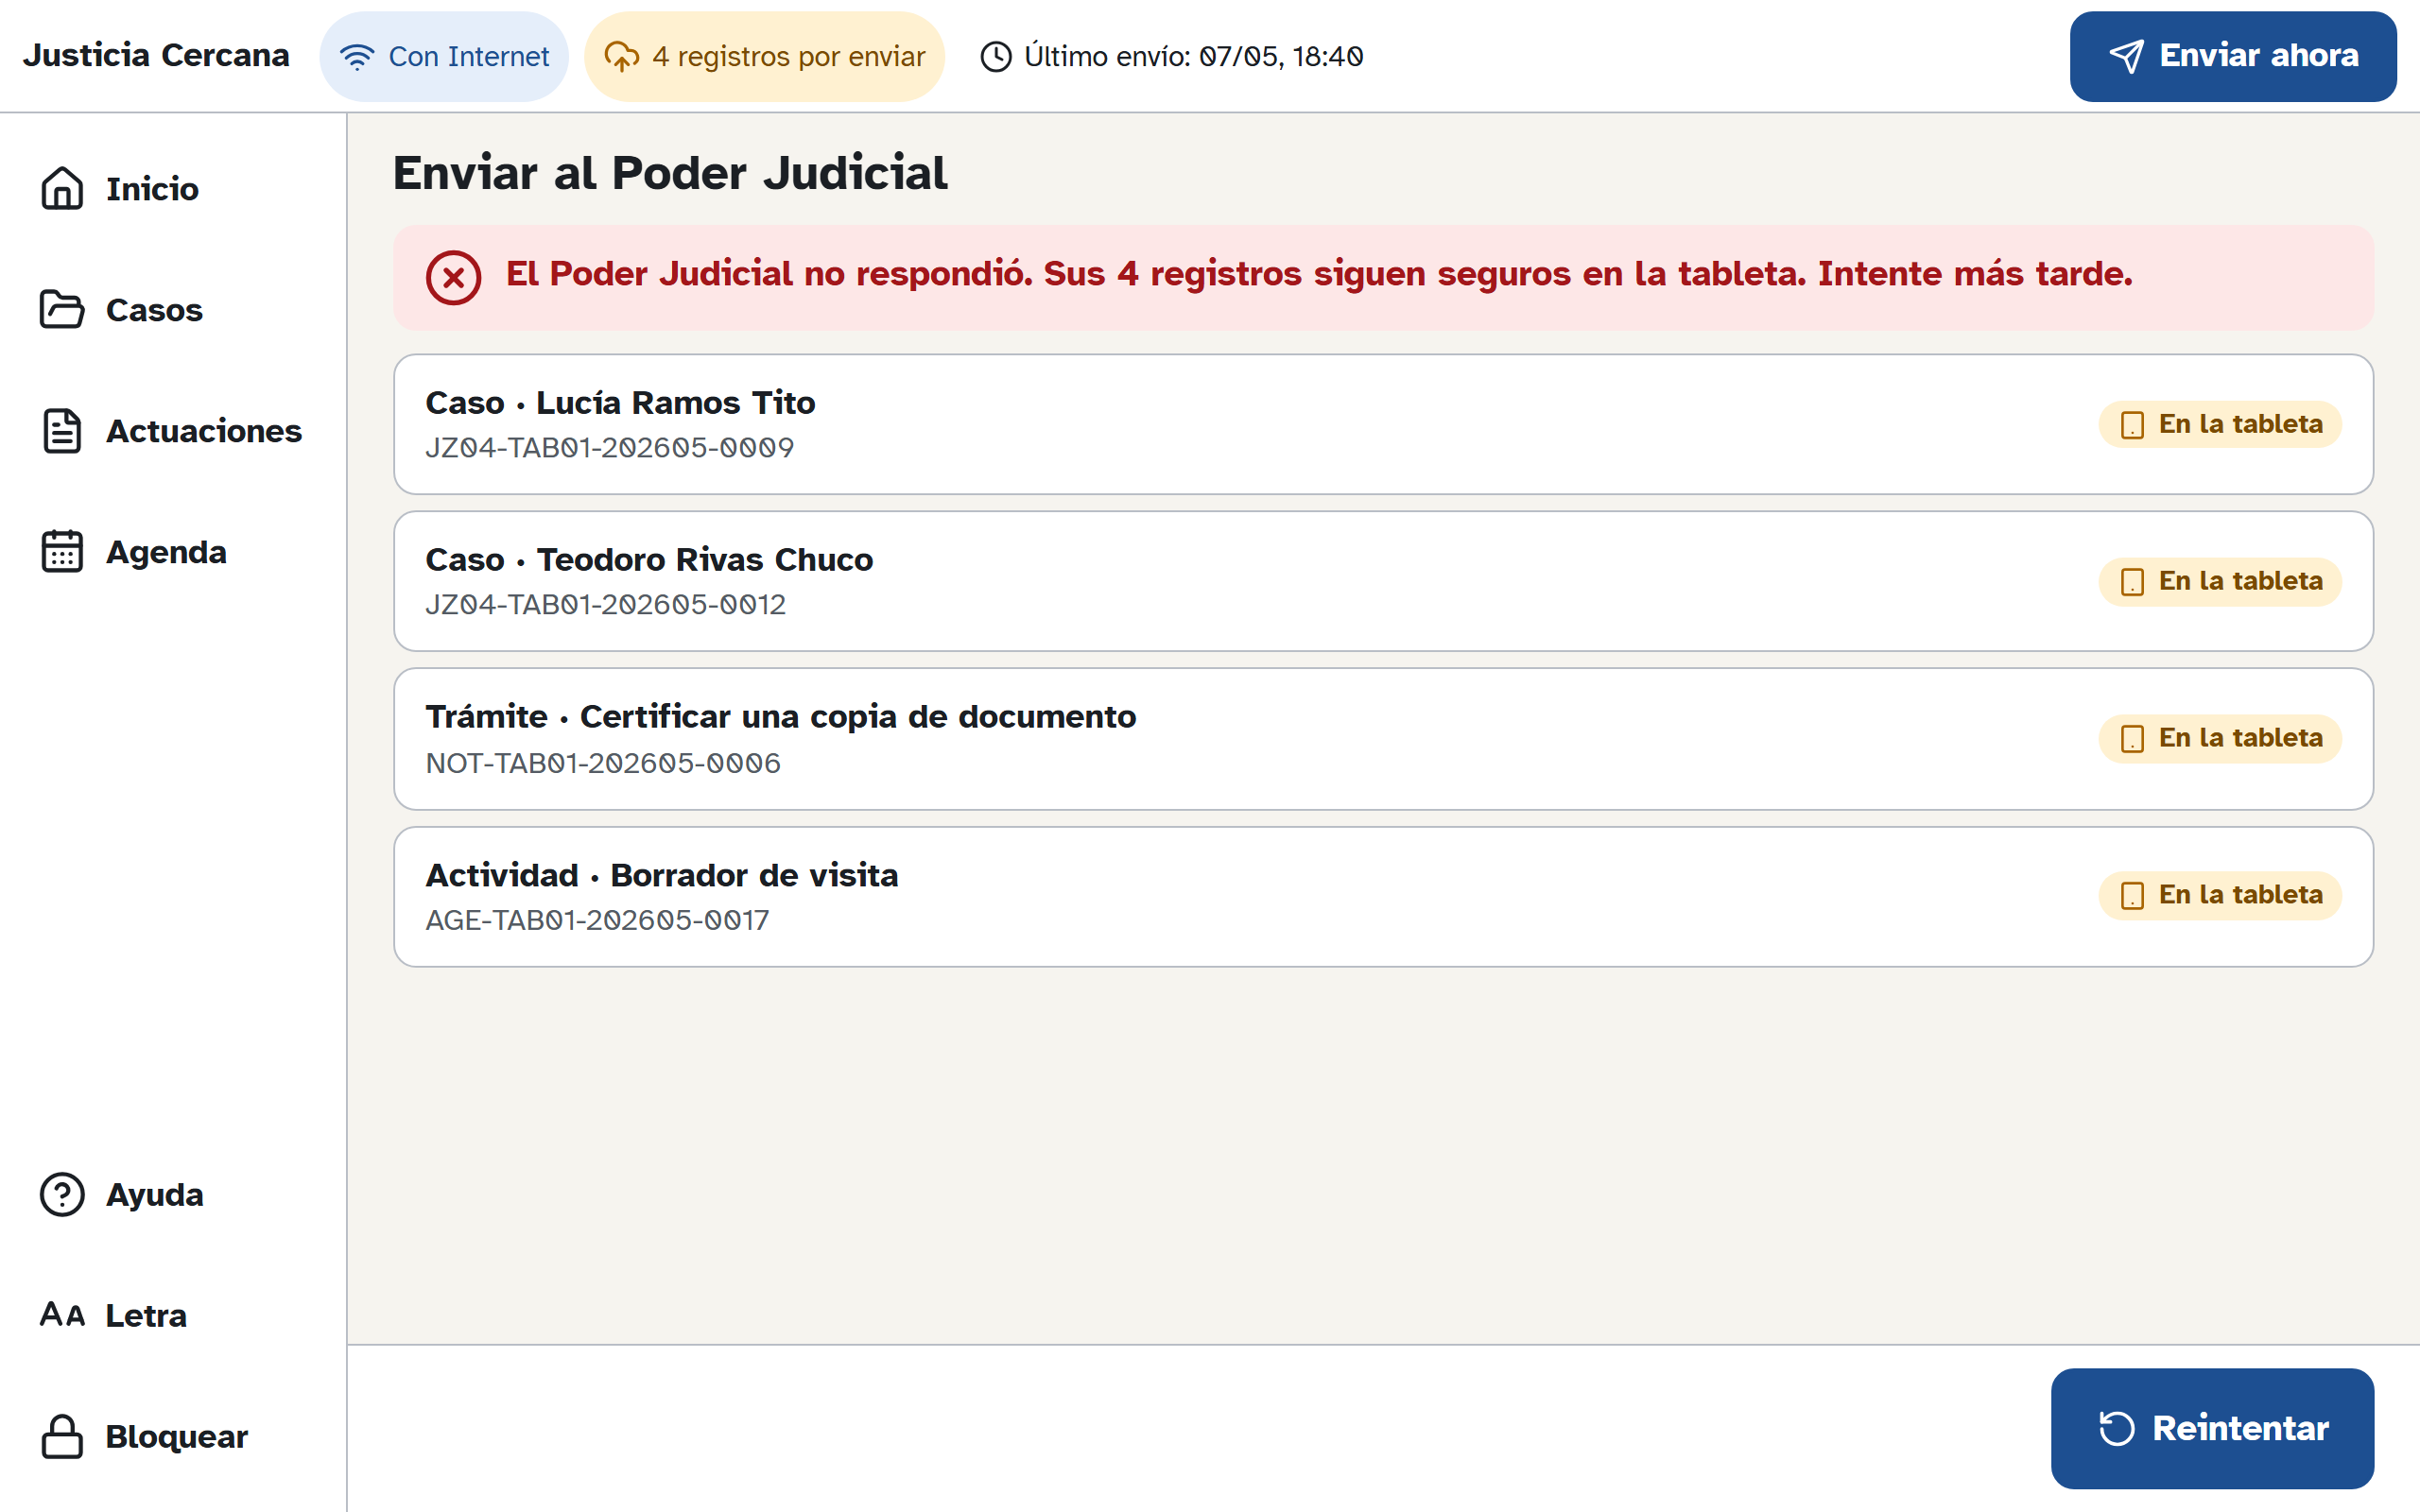
\includegraphics[width=\linewidth]{../../captures/F4-06b_error-servidor.png}\\[-2pt]{\footnotesize\raggedright\textbf{P-09 · 6.} Error del servidor: registros seguros en la tableta, [Reintentar] \emph{(Funcionamiento sin conexión)}\par}\end{minipage}\hfill
\begin{minipage}[t]{0.49\textwidth}\centering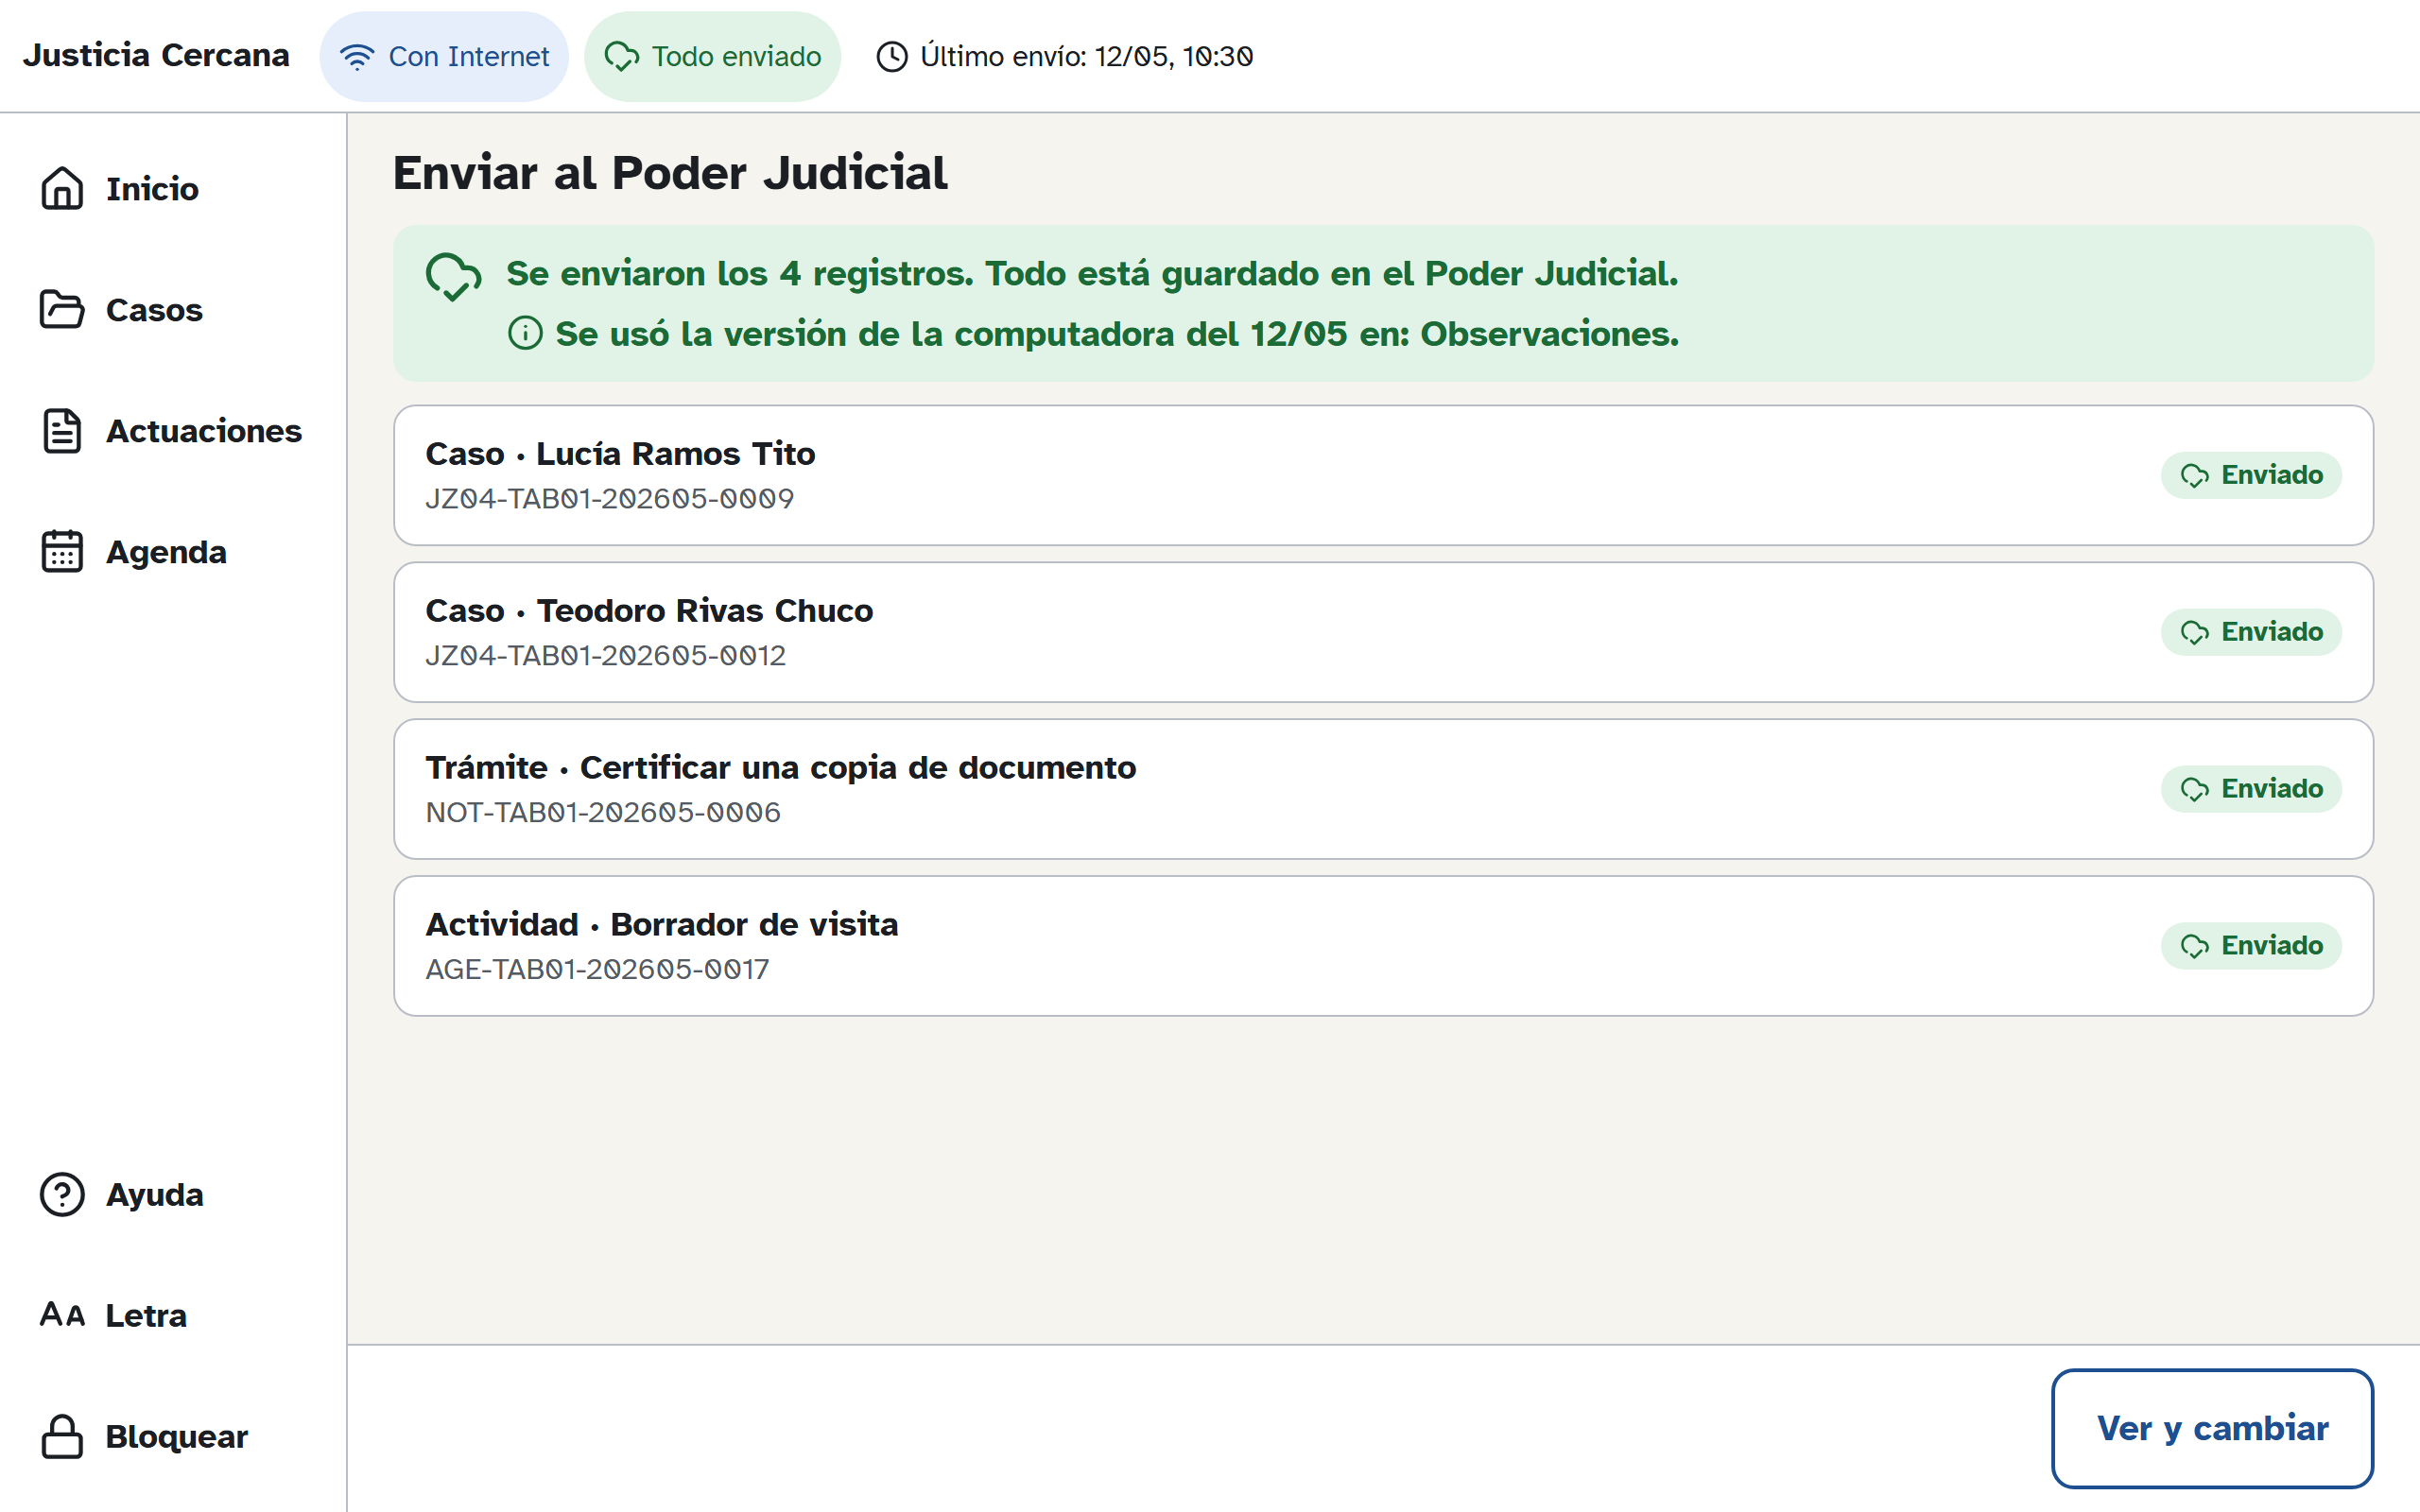
\includegraphics[width=\linewidth]{../../captures/F4-06c_conflicto-resuelto.png}\\[-2pt]{\footnotesize\raggedright\textbf{P-09 · 6.} Conflicto resuelto automáticamente con el cambio más reciente y aviso del campo \emph{(Funcionamiento sin conexión)}\par}\end{minipage}\par\vspace{8pt}\noindent
\begin{minipage}[t]{0.49\textwidth}\centering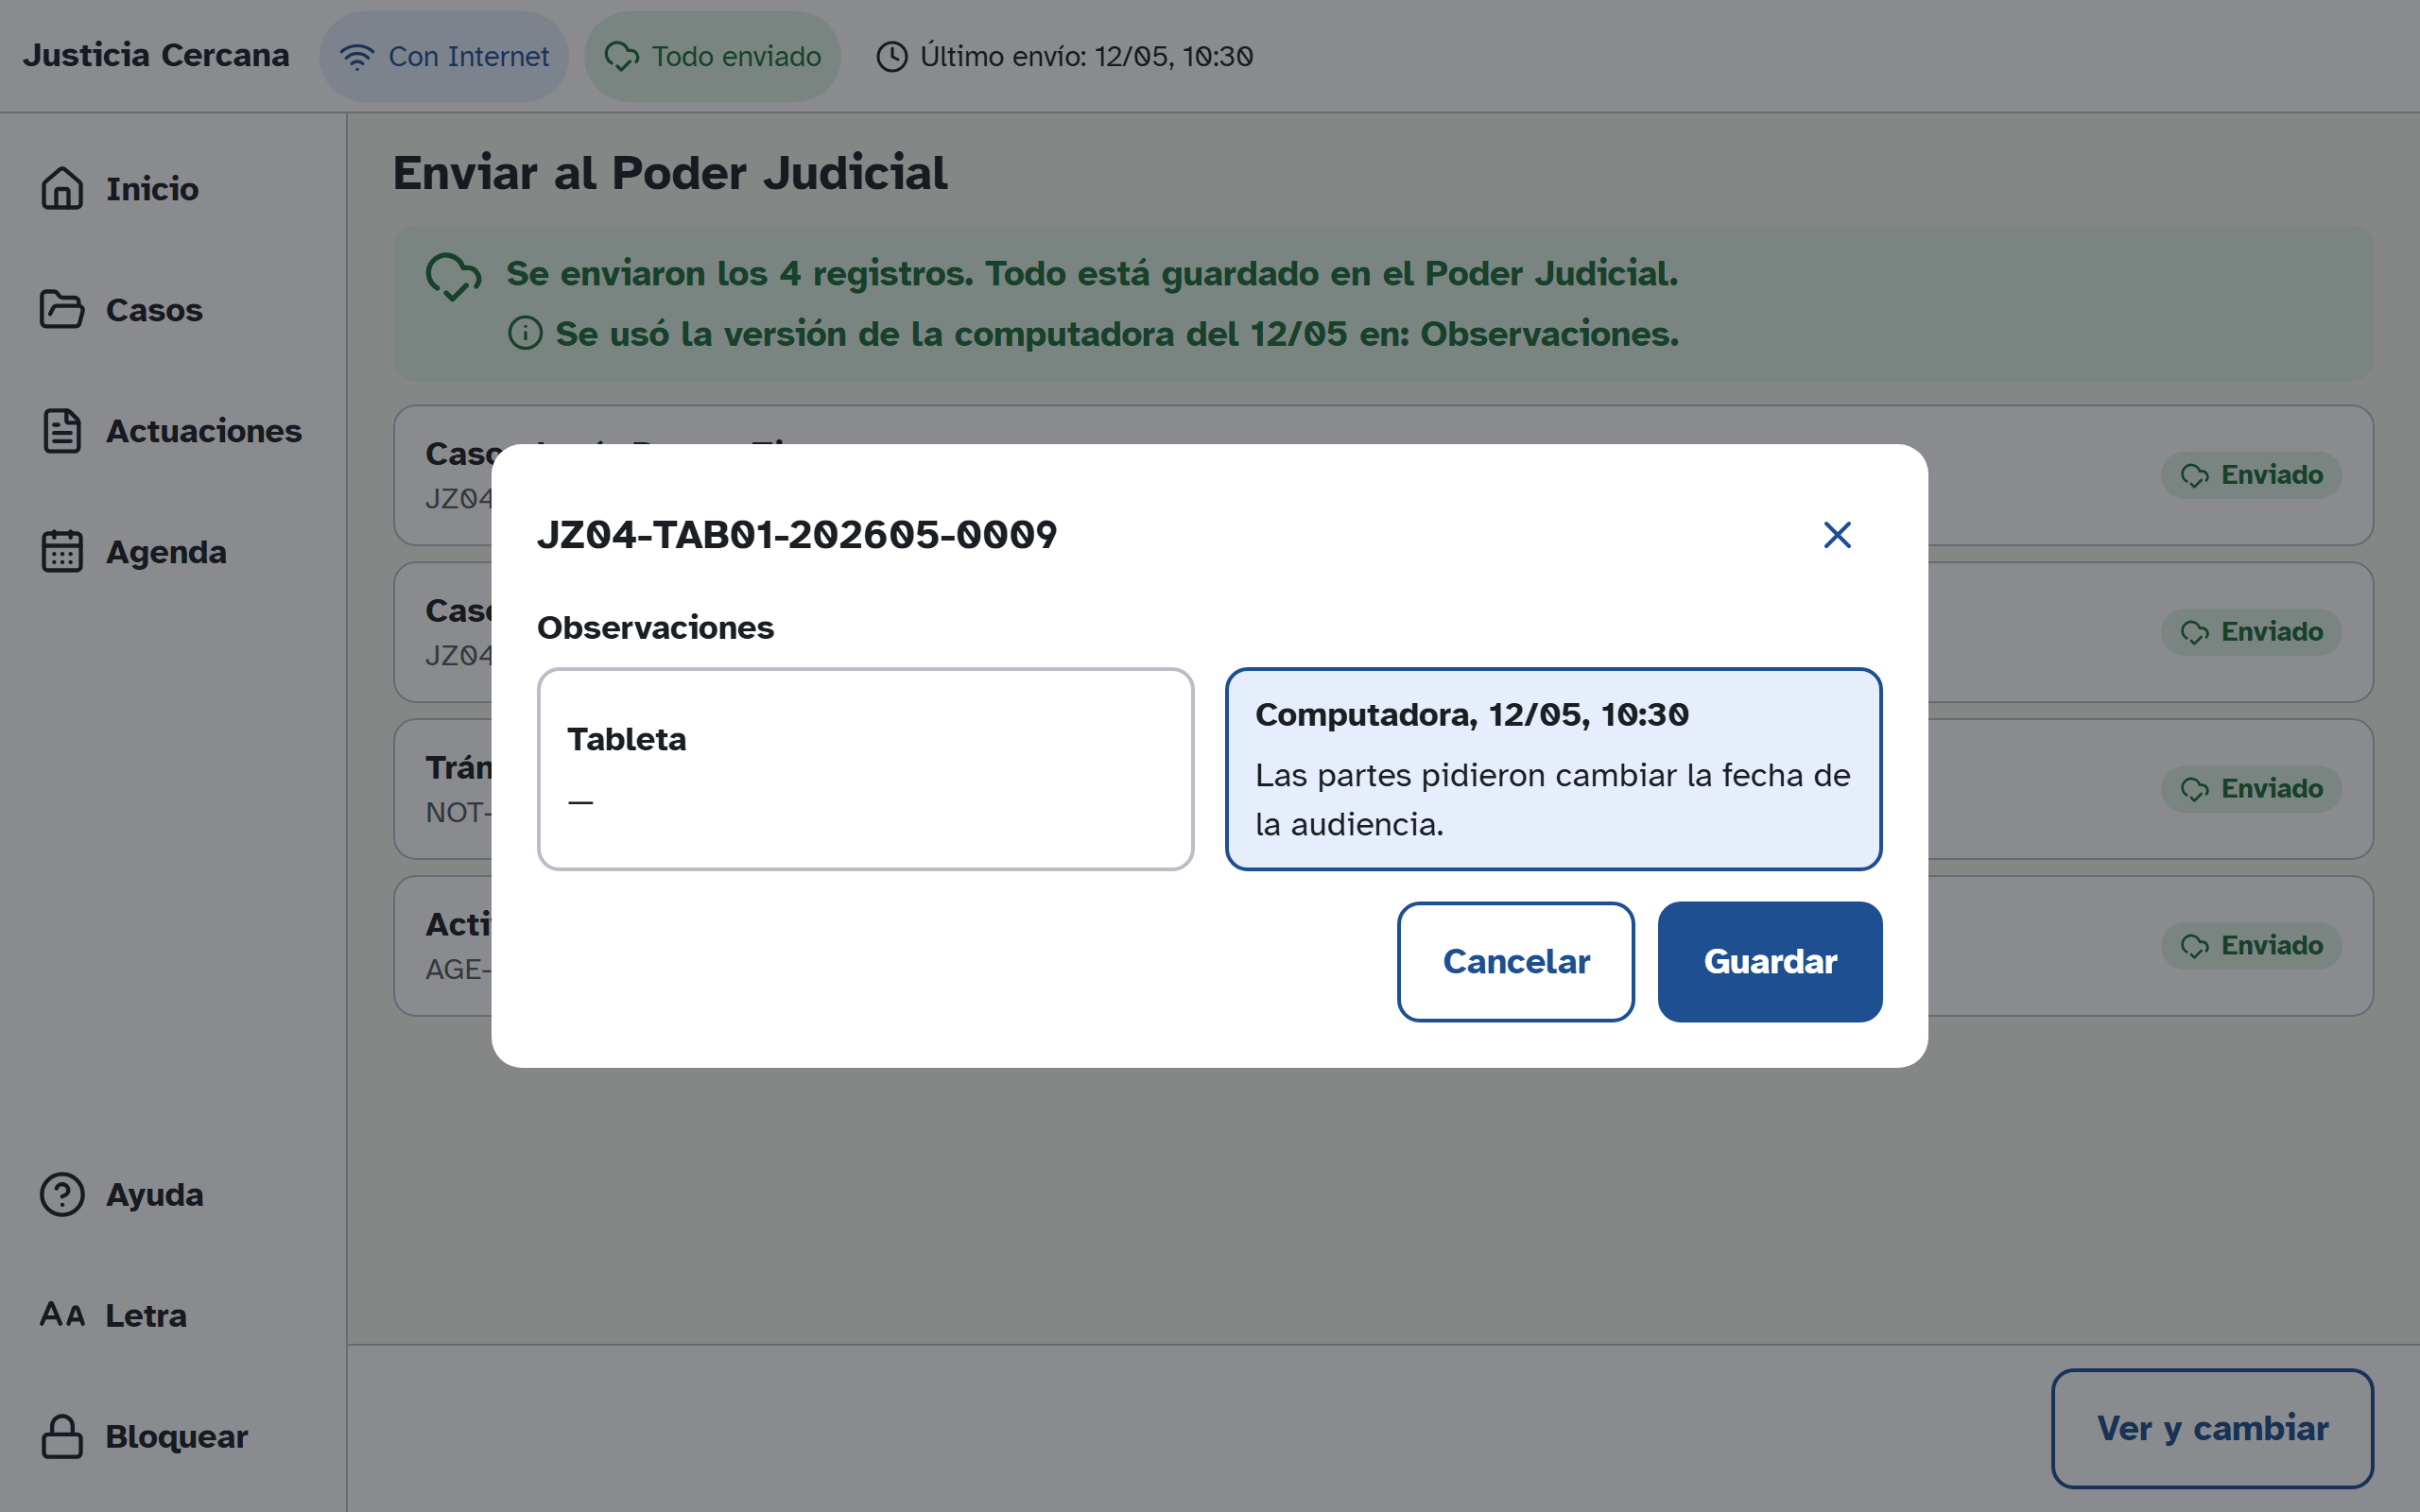
\includegraphics[width=\linewidth]{../../captures/F4-06d_ver-y-cambiar.png}\\[-2pt]{\footnotesize\raggedright\textbf{P-09 · 6.} [Ver y cambiar]: comparación por campo tableta / computadora \emph{(Funcionamiento sin conexión)}\par}\end{minipage}\hfill
\par\vspace{4pt}
\subsection*{Flujo A}
\noindent
\begin{minipage}[t]{0.49\textwidth}\centering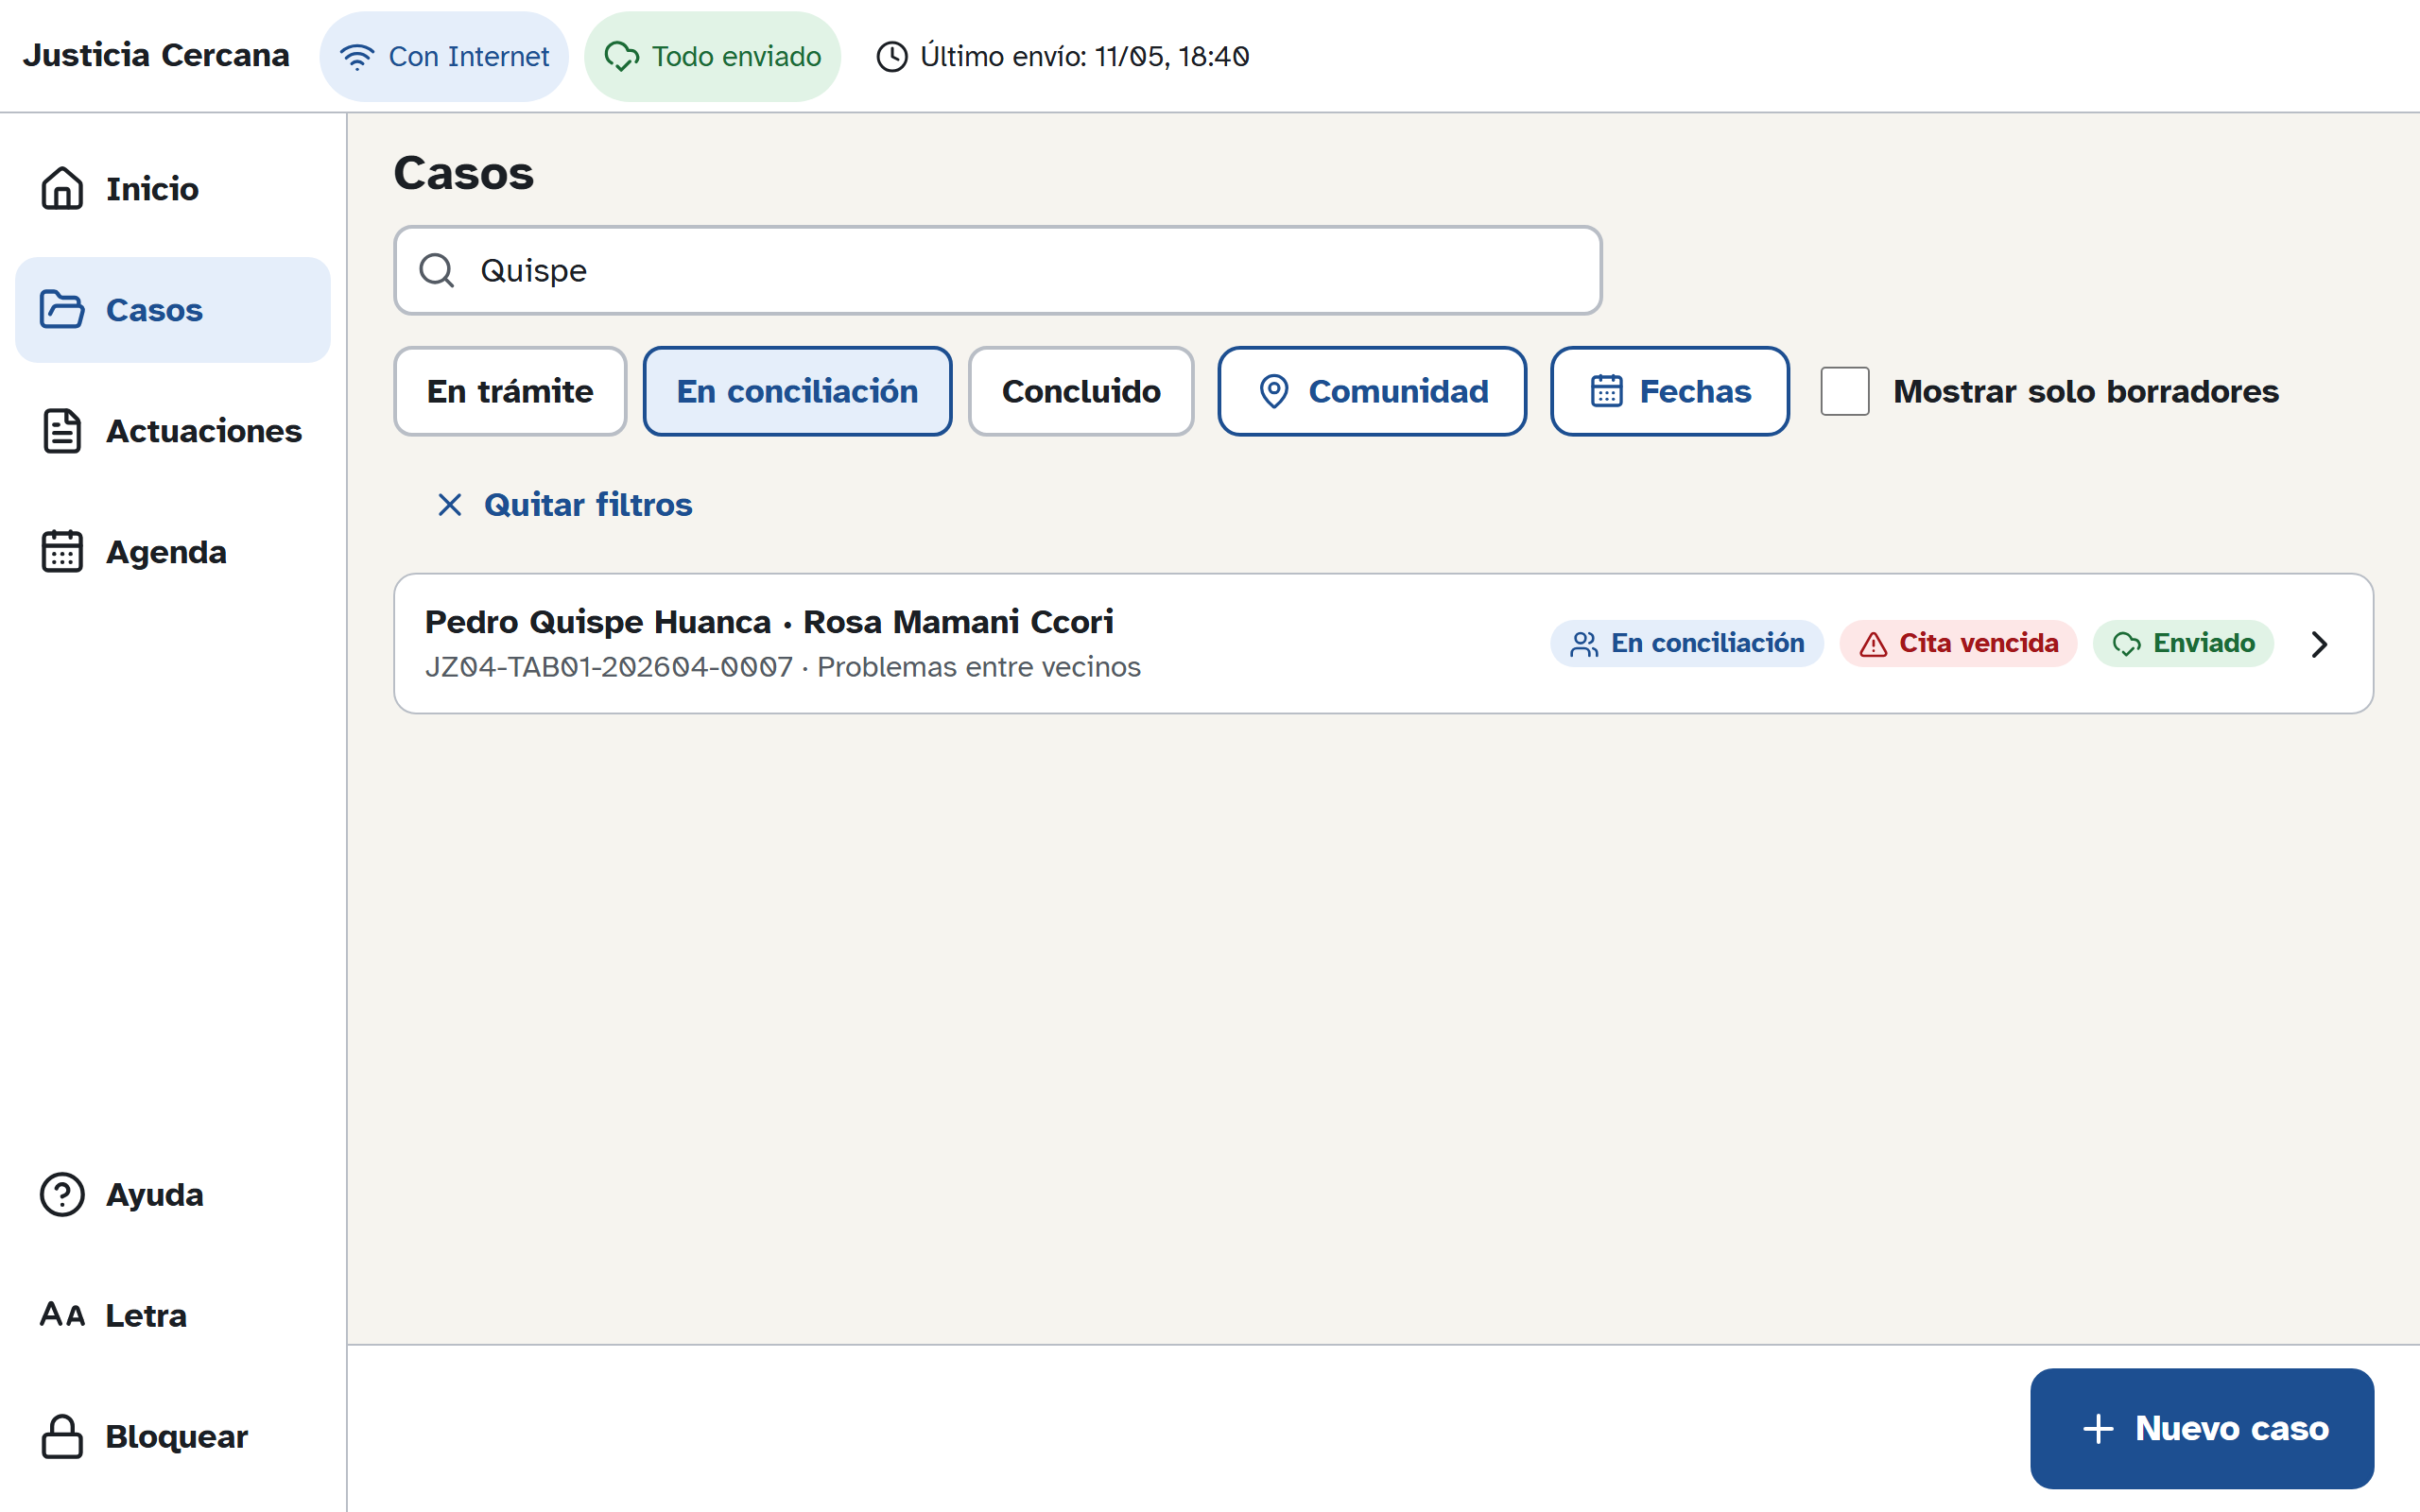
\includegraphics[width=\linewidth]{../../captures/FA-01_busqueda-filtro.png}\\[-2pt]{\footnotesize\raggedright\textbf{P-02 · 1.} Búsqueda ``Quispe'' + filtro En conciliación; motivo de atención en texto \emph{(Cobertura y funcionamiento de los módulos)}\par}\end{minipage}\hfill
\begin{minipage}[t]{0.49\textwidth}\centering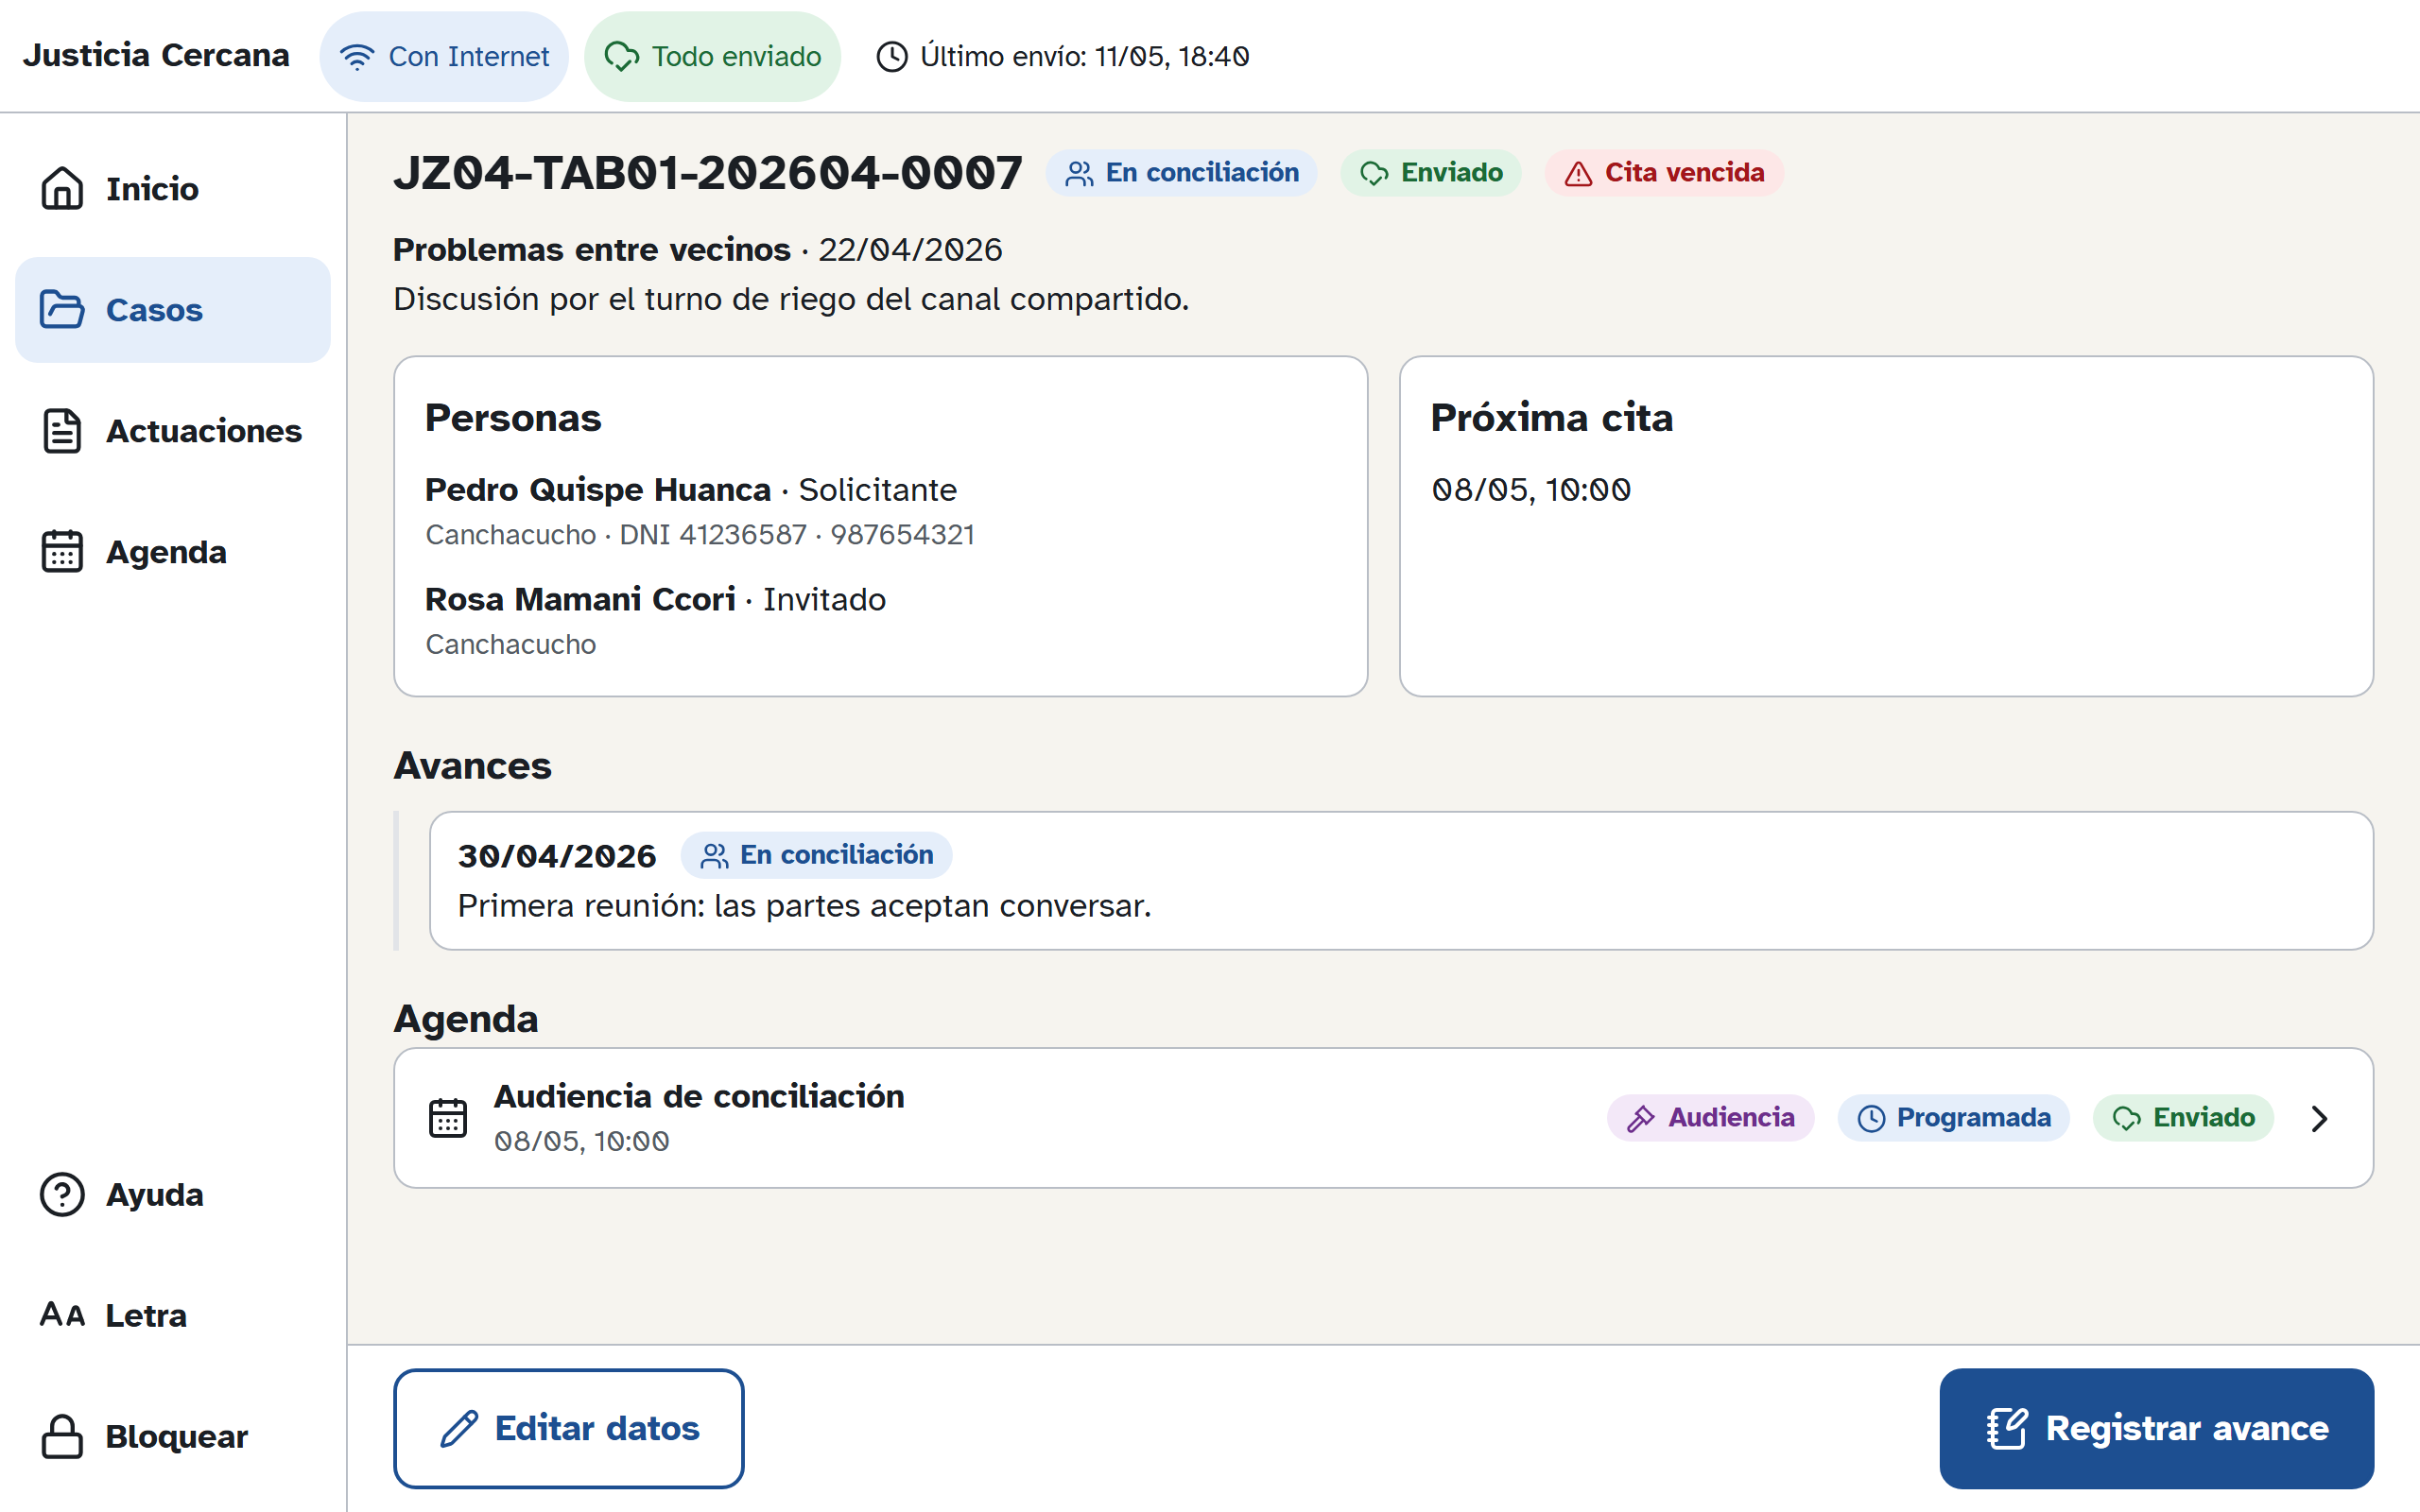
\includegraphics[width=\linewidth]{../../captures/FA-02_caso-cita-vencida.png}\\[-2pt]{\footnotesize\raggedright\textbf{P-04 · 2.} Detalle con ``Cita vencida'', distintivo, partes, historial \emph{(Cobertura y funcionamiento de los módulos)}\par}\end{minipage}\par\vspace{8pt}\noindent
\begin{minipage}[t]{0.49\textwidth}\centering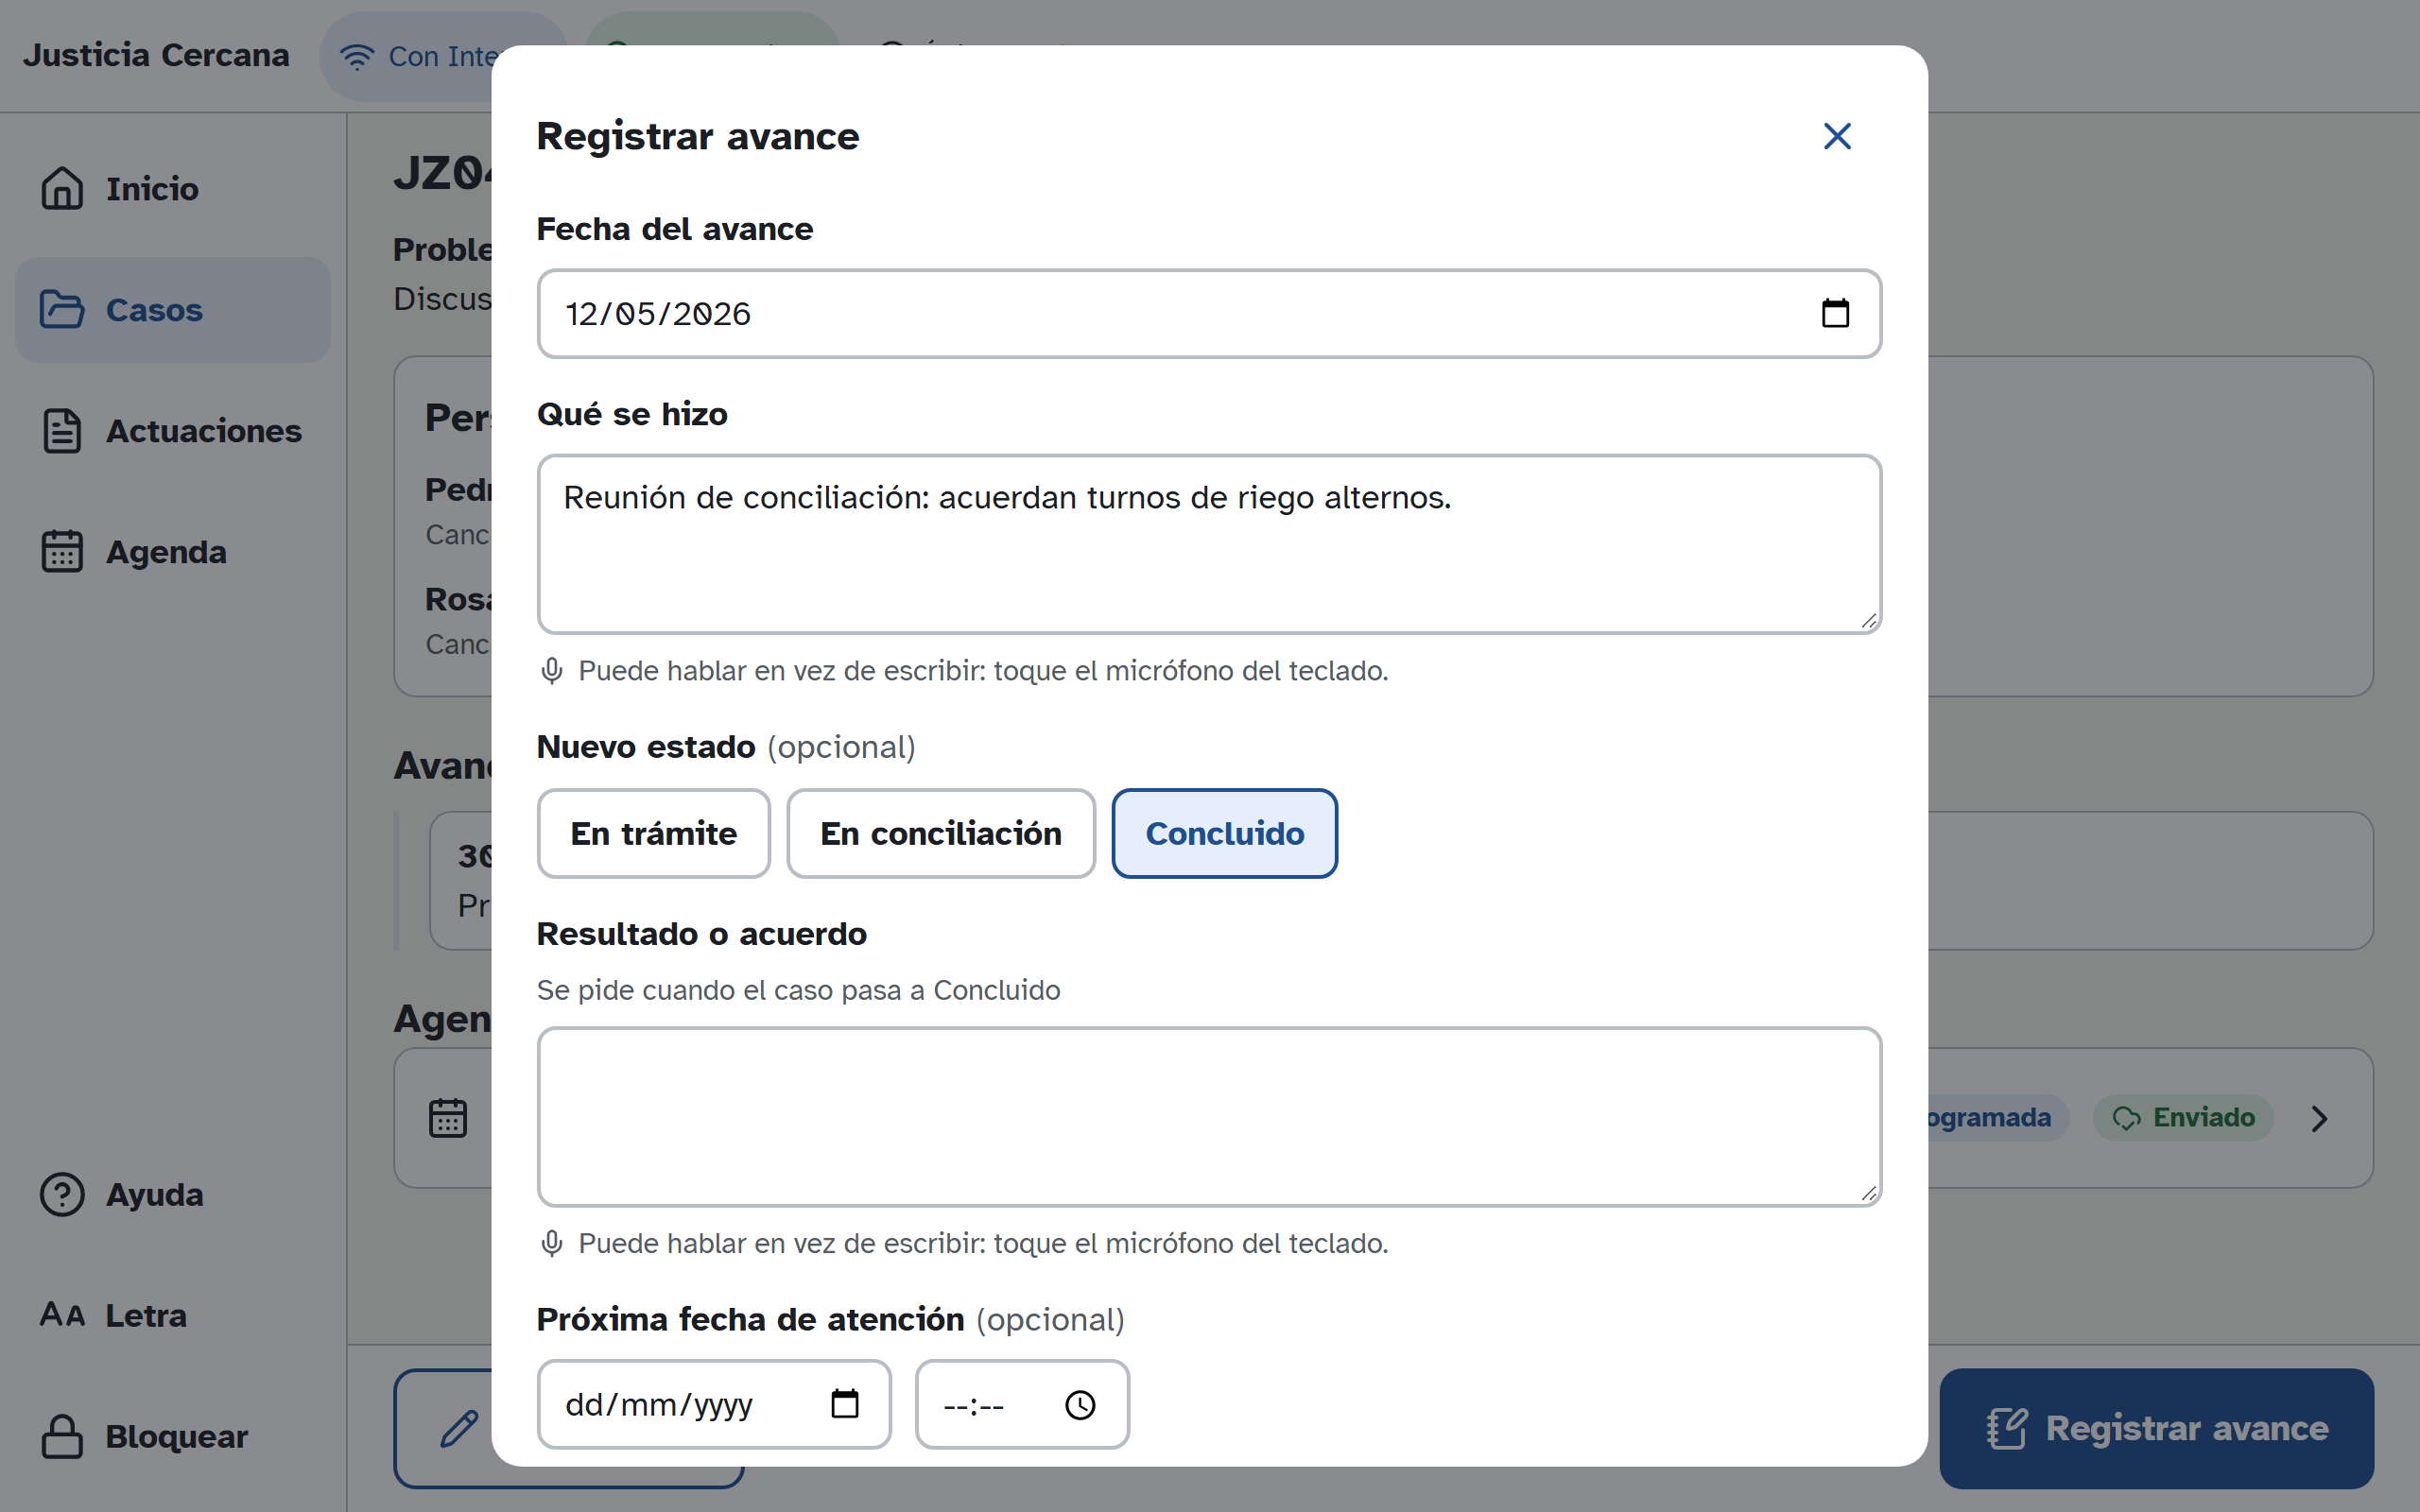
\includegraphics[width=\linewidth]{../../captures/FA-03a_registrar-avance.png}\\[-2pt]{\footnotesize\raggedright\textbf{P-04 · 3.} Ventana ``Registrar avance'' con condicional de acuerdo al pasar a Concluido \emph{(Cobertura y funcionamiento de los módulos)}\par}\end{minipage}\hfill
\begin{minipage}[t]{0.49\textwidth}\centering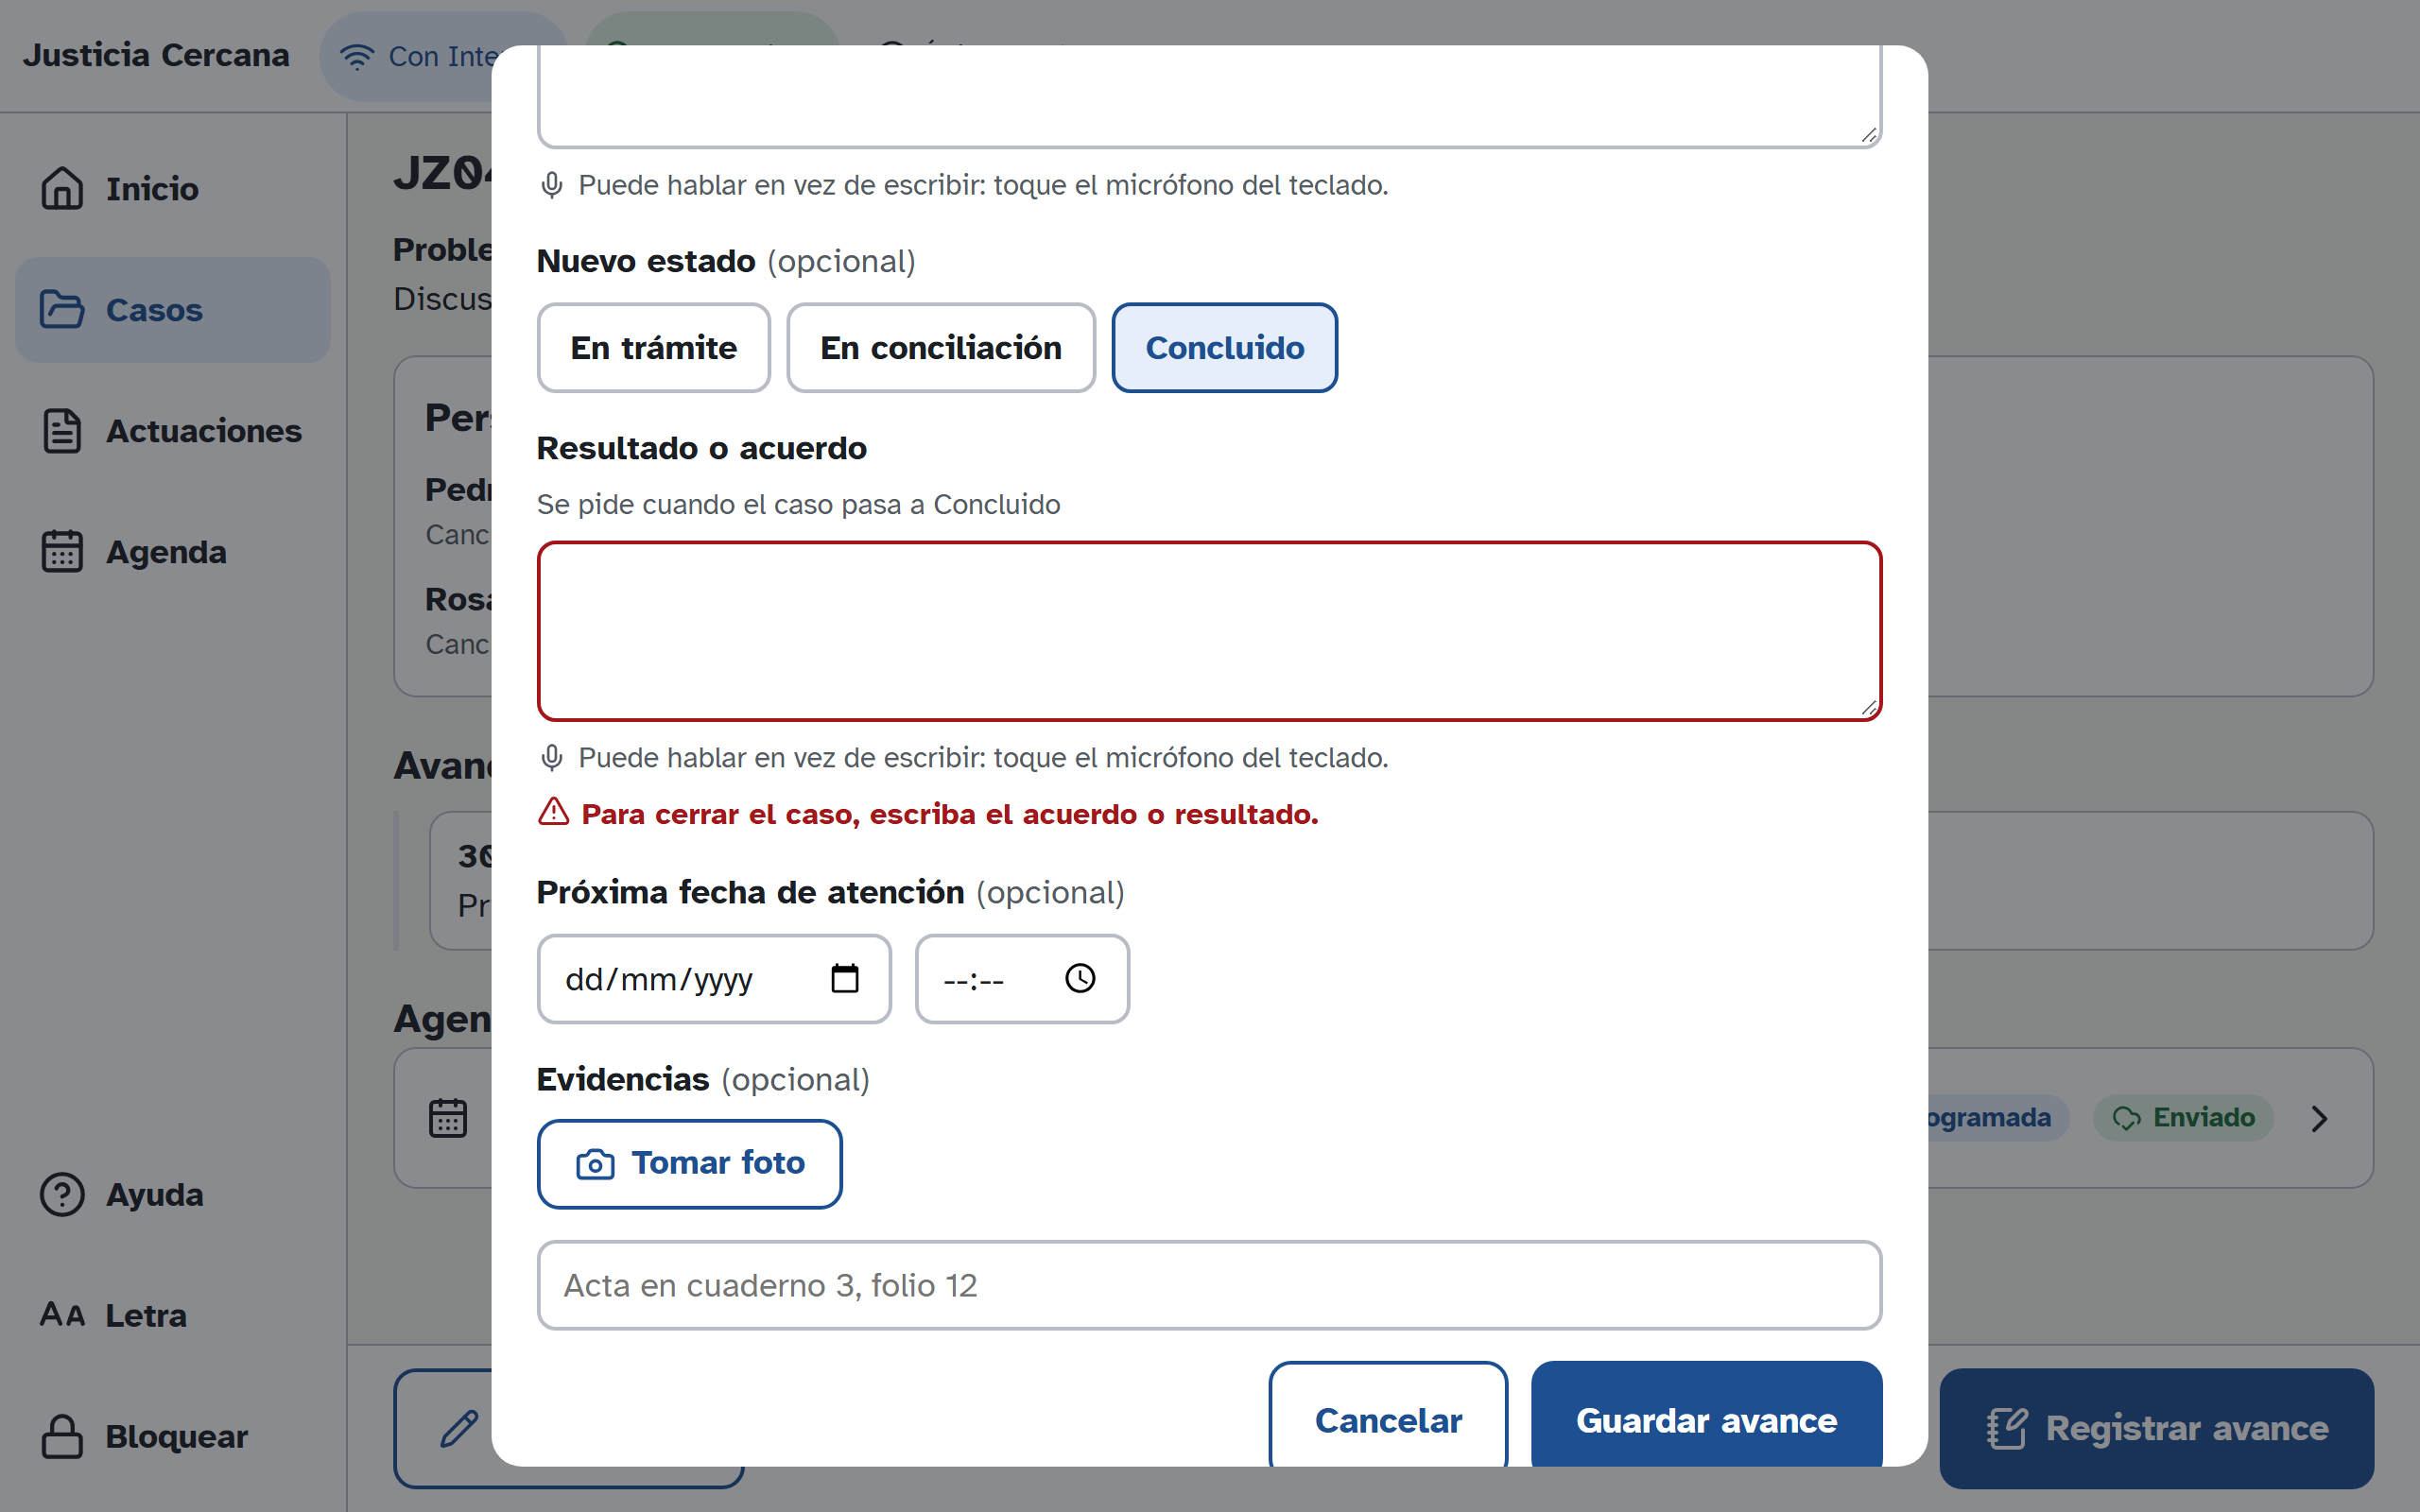
\includegraphics[width=\linewidth]{../../captures/FA-03b_exige-acuerdo.png}\\[-2pt]{\footnotesize\raggedright\textbf{P-04 · 3.} Concluido exige el acuerdo (mensaje en lenguaje simple) \emph{(Principios de diseño y heurísticas)}\par}\end{minipage}\par\vspace{8pt}\noindent
\begin{minipage}[t]{0.49\textwidth}\centering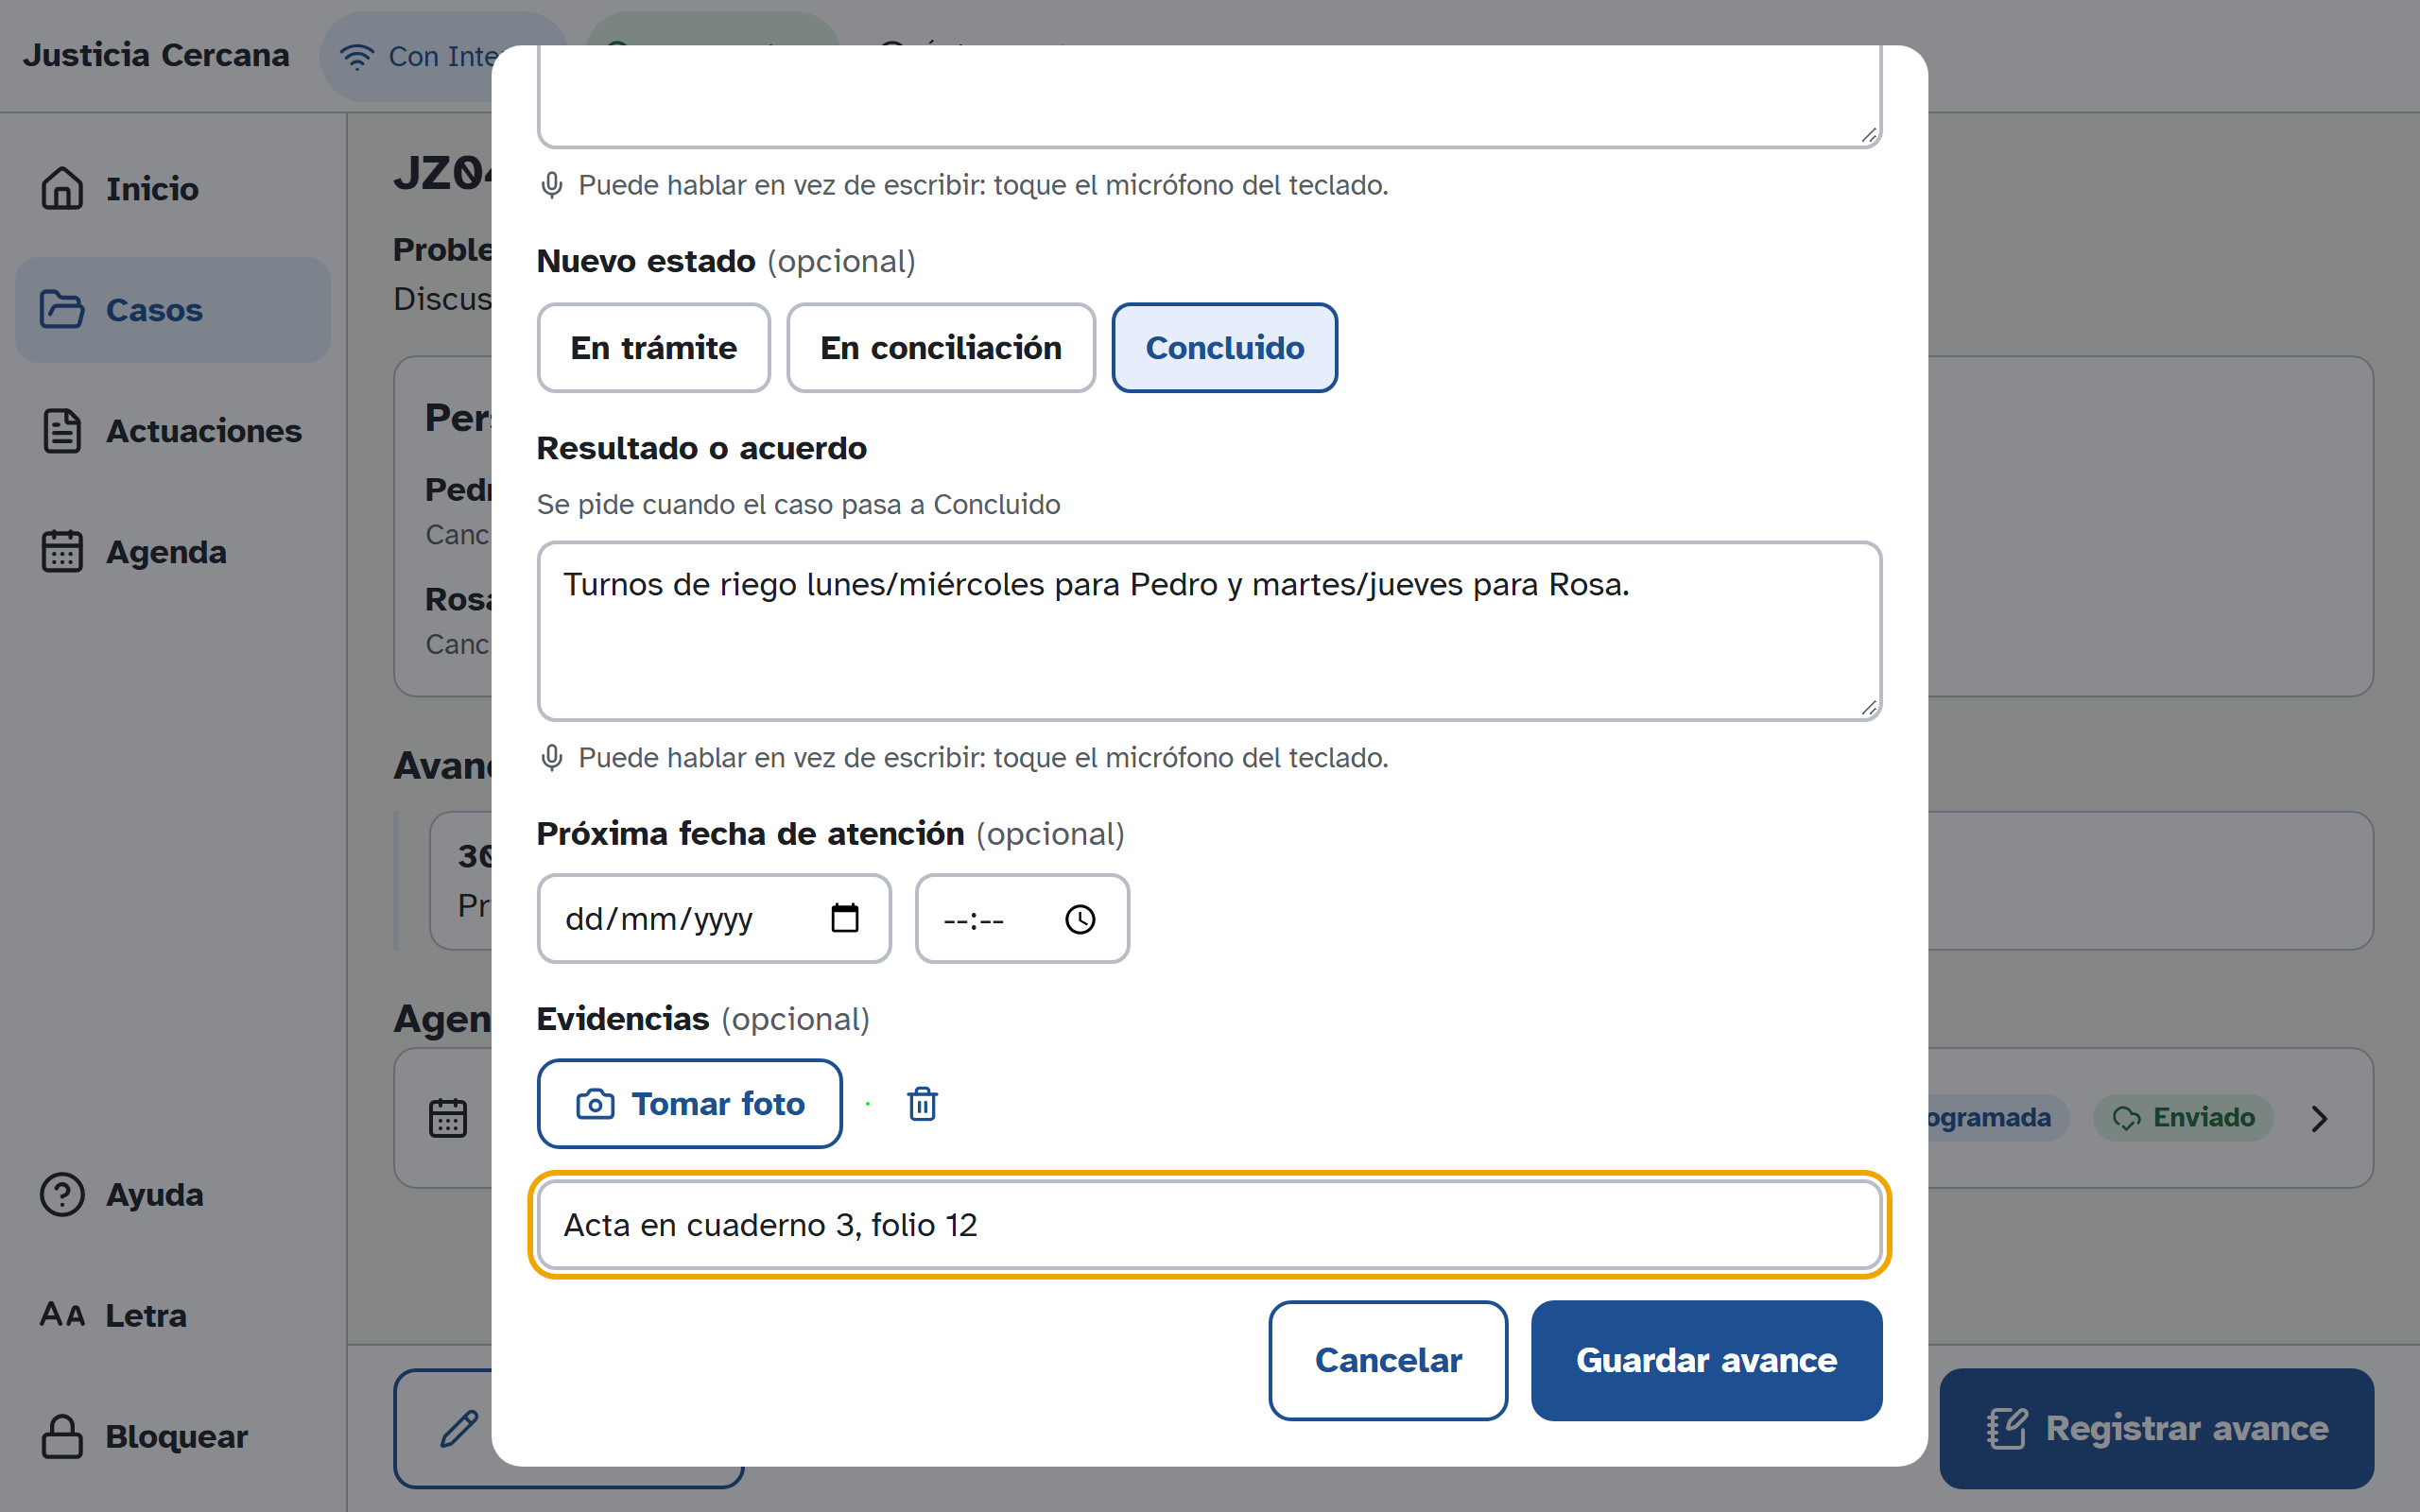
\includegraphics[width=\linewidth]{../../captures/FA-03c_foto-acta.png}\\[-2pt]{\footnotesize\raggedright\textbf{P-04 · 3.} Acuerdo escrito y foto del acta adjunta + referencia física \emph{(Cobertura y funcionamiento de los módulos)}\par}\end{minipage}\hfill
\begin{minipage}[t]{0.49\textwidth}\centering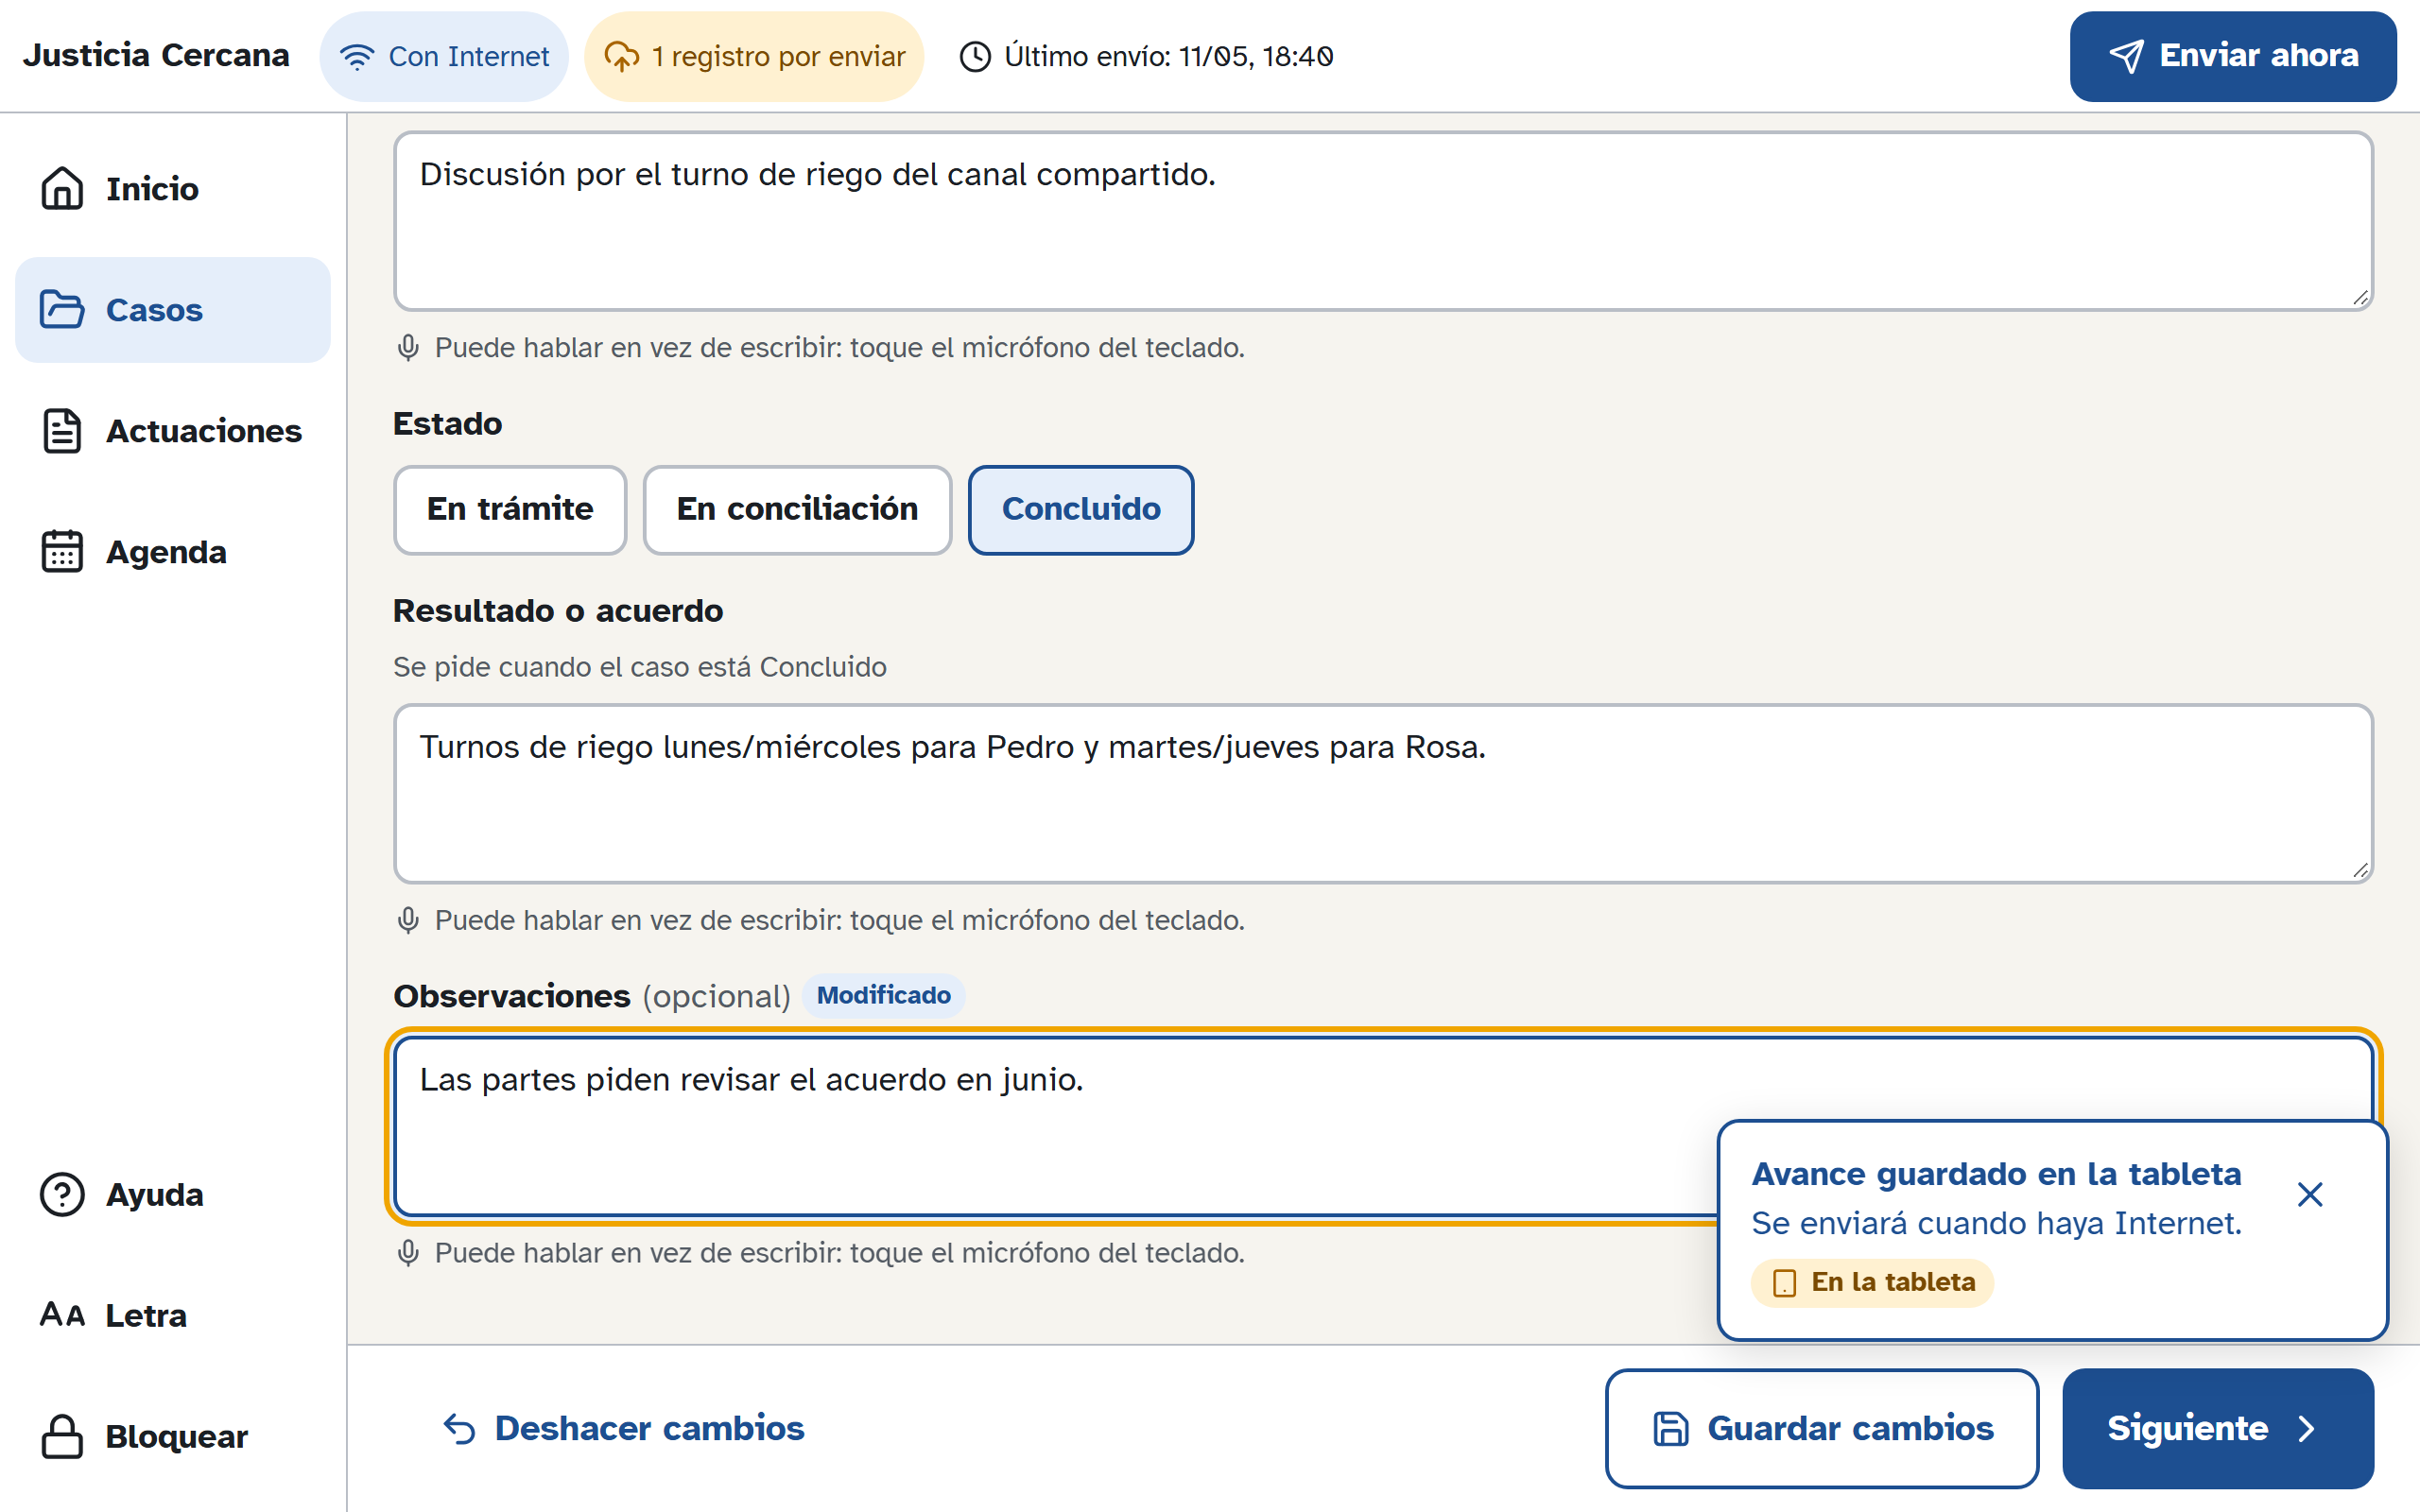
\includegraphics[width=\linewidth]{../../captures/FA-04a_modificado.png}\\[-2pt]{\footnotesize\raggedright\textbf{P-03 · 4.} Campo editado resaltado con ``Modificado'' y botón [Deshacer cambios] \emph{(Principios de diseño y heurísticas)}\par}\end{minipage}\par\vspace{8pt}\noindent
\begin{minipage}[t]{0.49\textwidth}\centering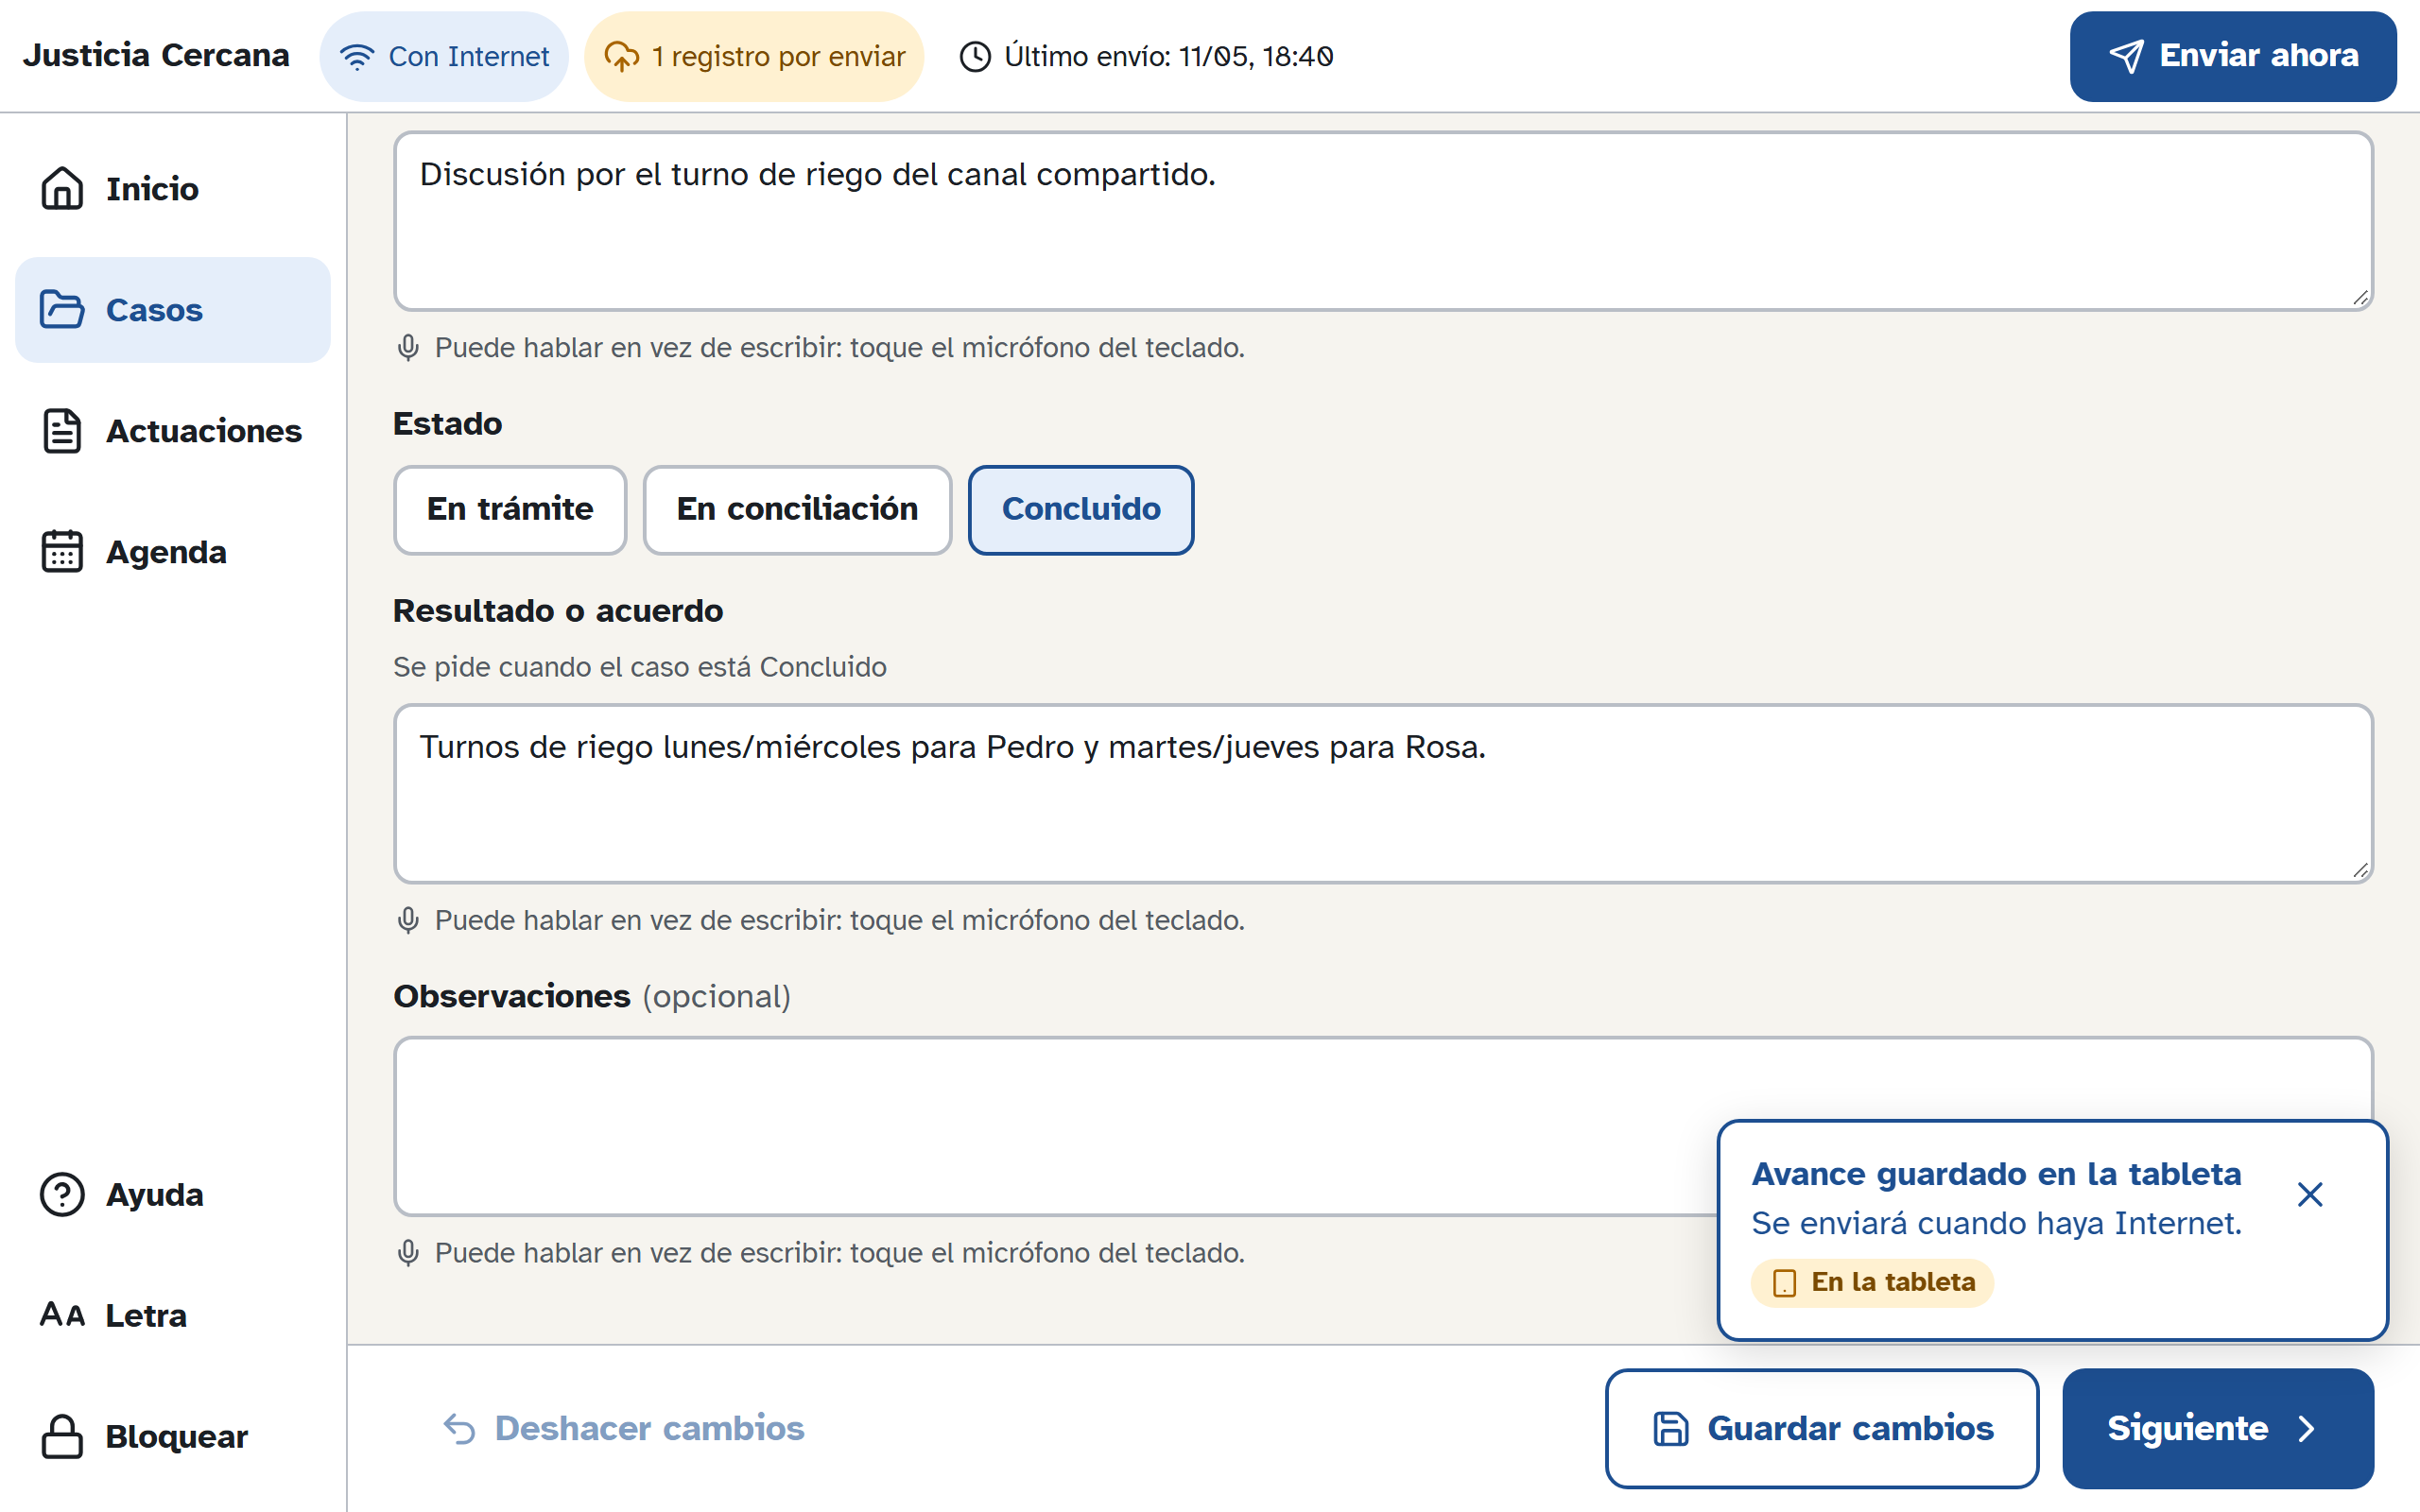
\includegraphics[width=\linewidth]{../../captures/FA-04b_deshacer.png}\\[-2pt]{\footnotesize\raggedright\textbf{P-03 · 4.} [Deshacer cambios] devuelve el valor original \emph{(Principios de diseño y heurísticas)}\par}\end{minipage}\hfill
\begin{minipage}[t]{0.49\textwidth}\centering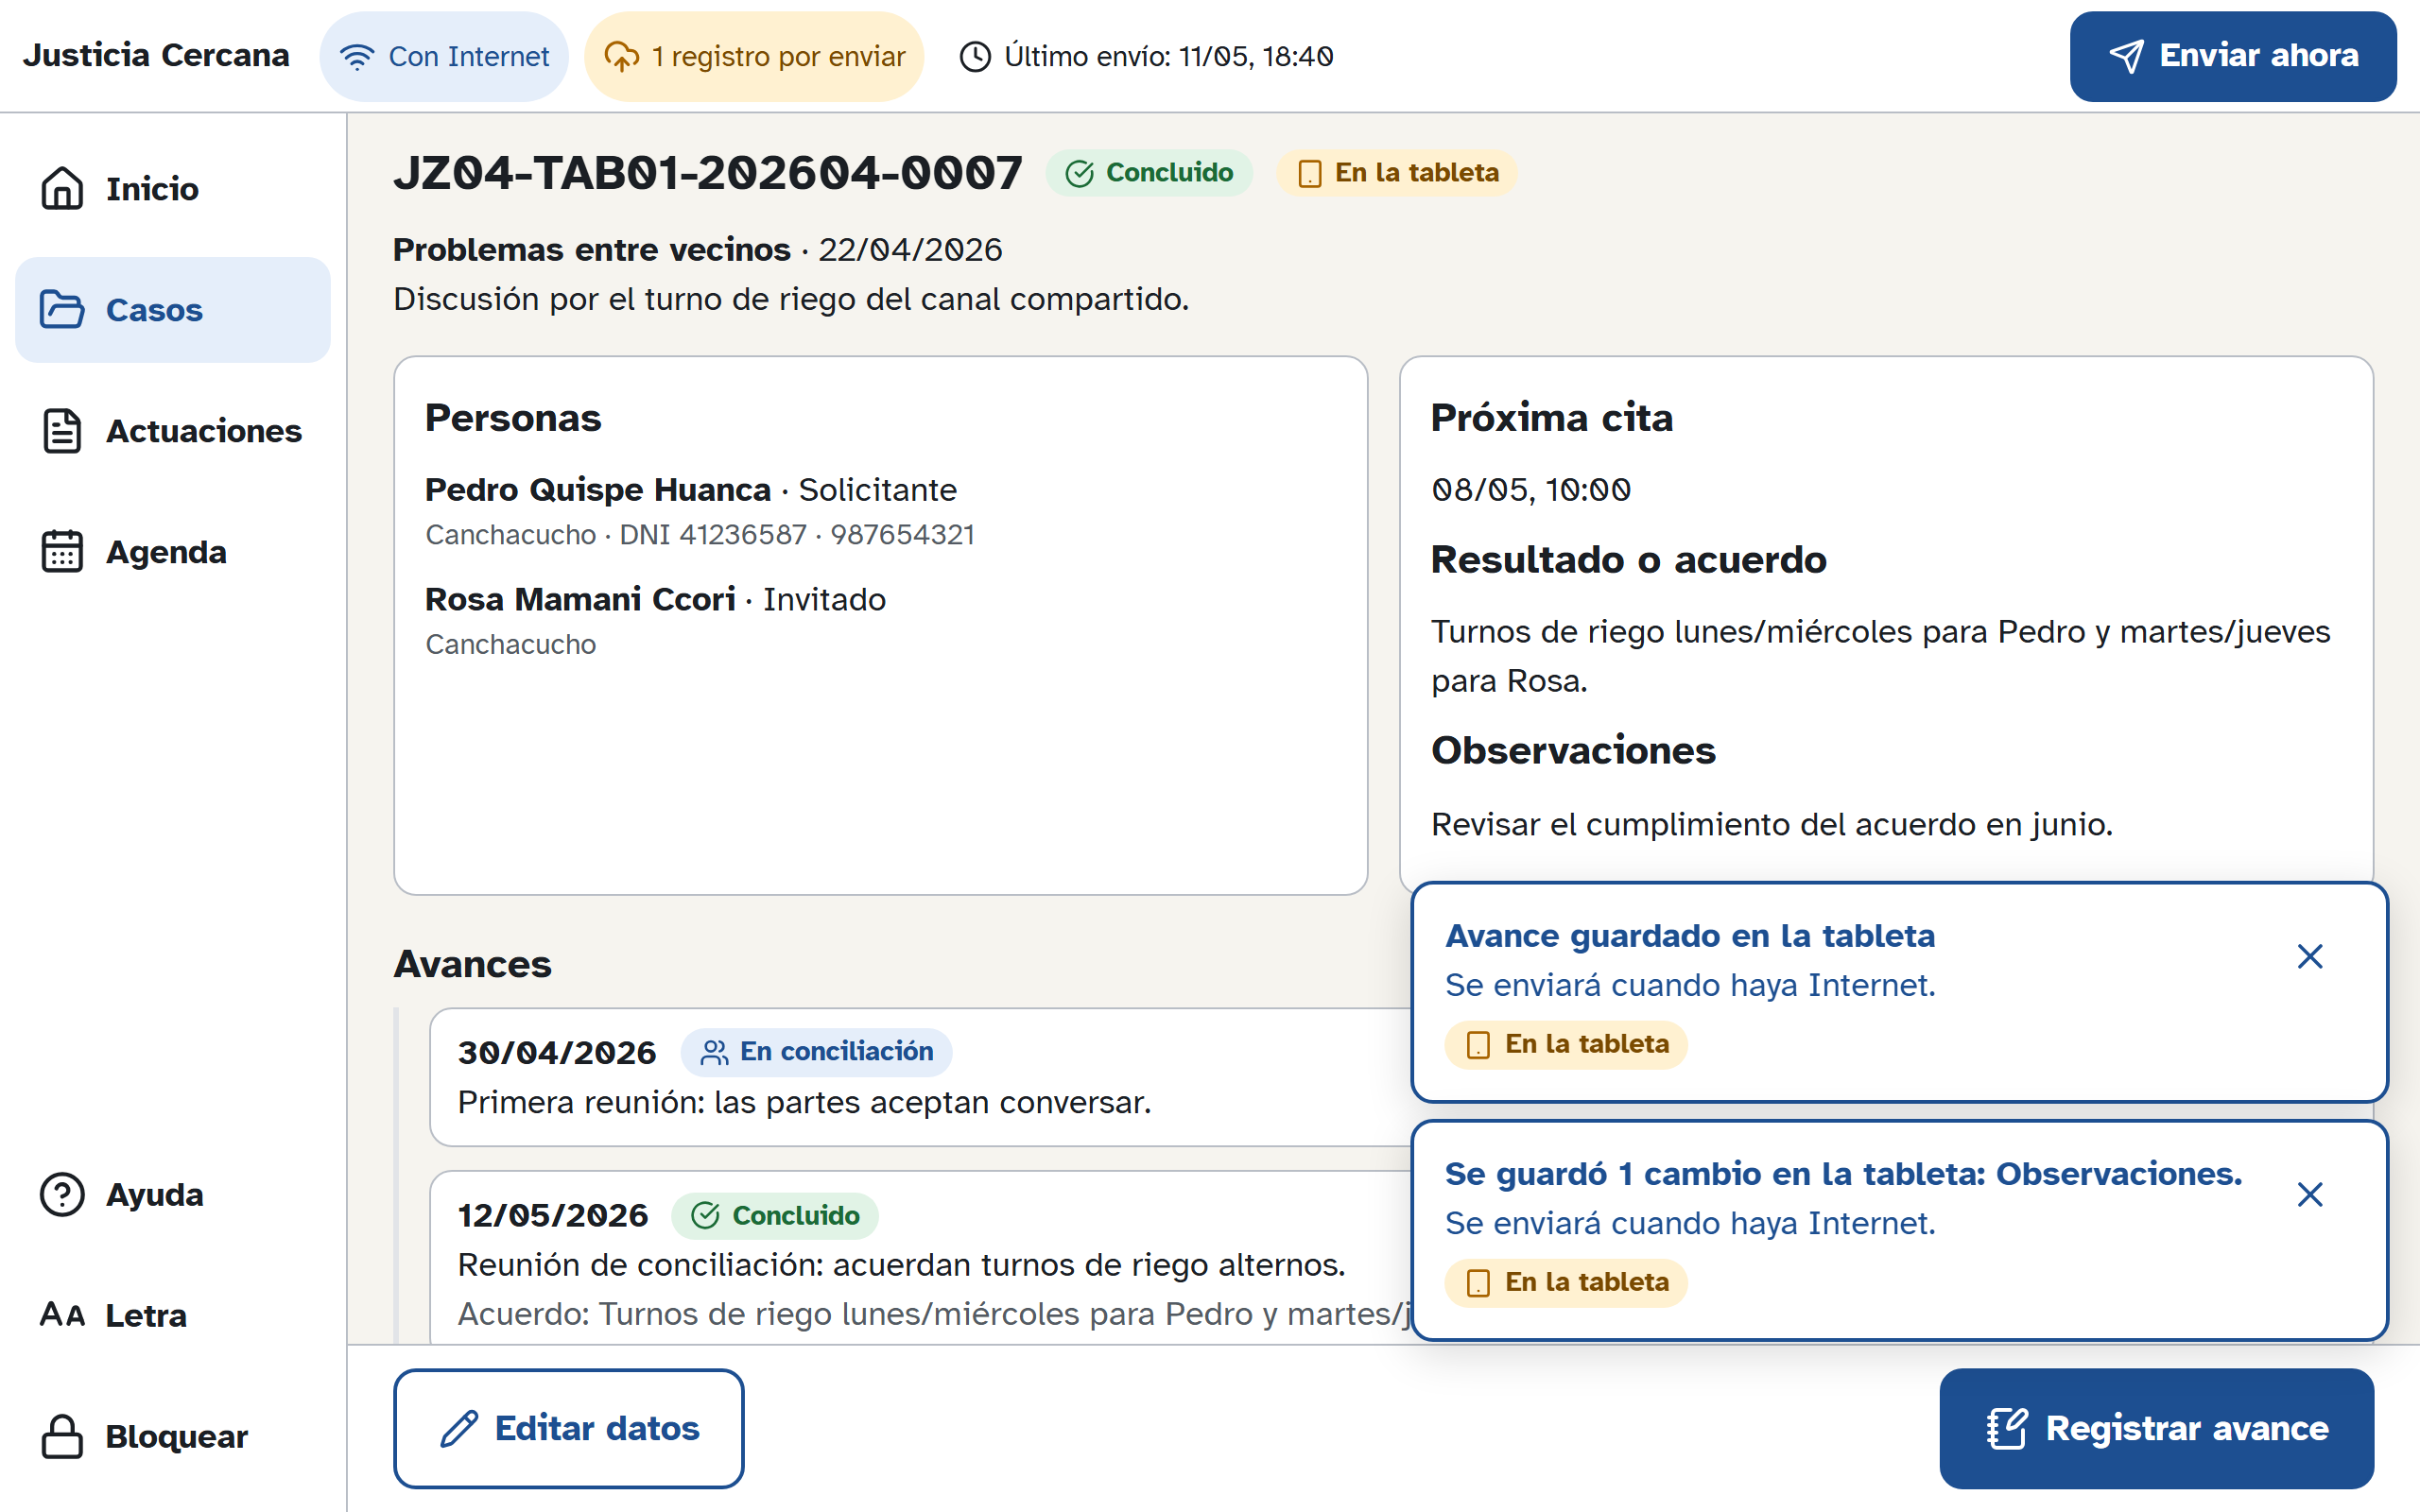
\includegraphics[width=\linewidth]{../../captures/FA-04c_confirmacion-cambios.png}\\[-2pt]{\footnotesize\raggedright\textbf{P-04 · 4.} ``Se guardó 1 cambio en la tableta: Observaciones.'' \emph{(Funcionamiento sin conexión)}\par}\end{minipage}\par\vspace{8pt}\noindent
\par\vspace{4pt}
\subsection*{Flujo B}
\noindent
\begin{minipage}[t]{0.49\textwidth}\centering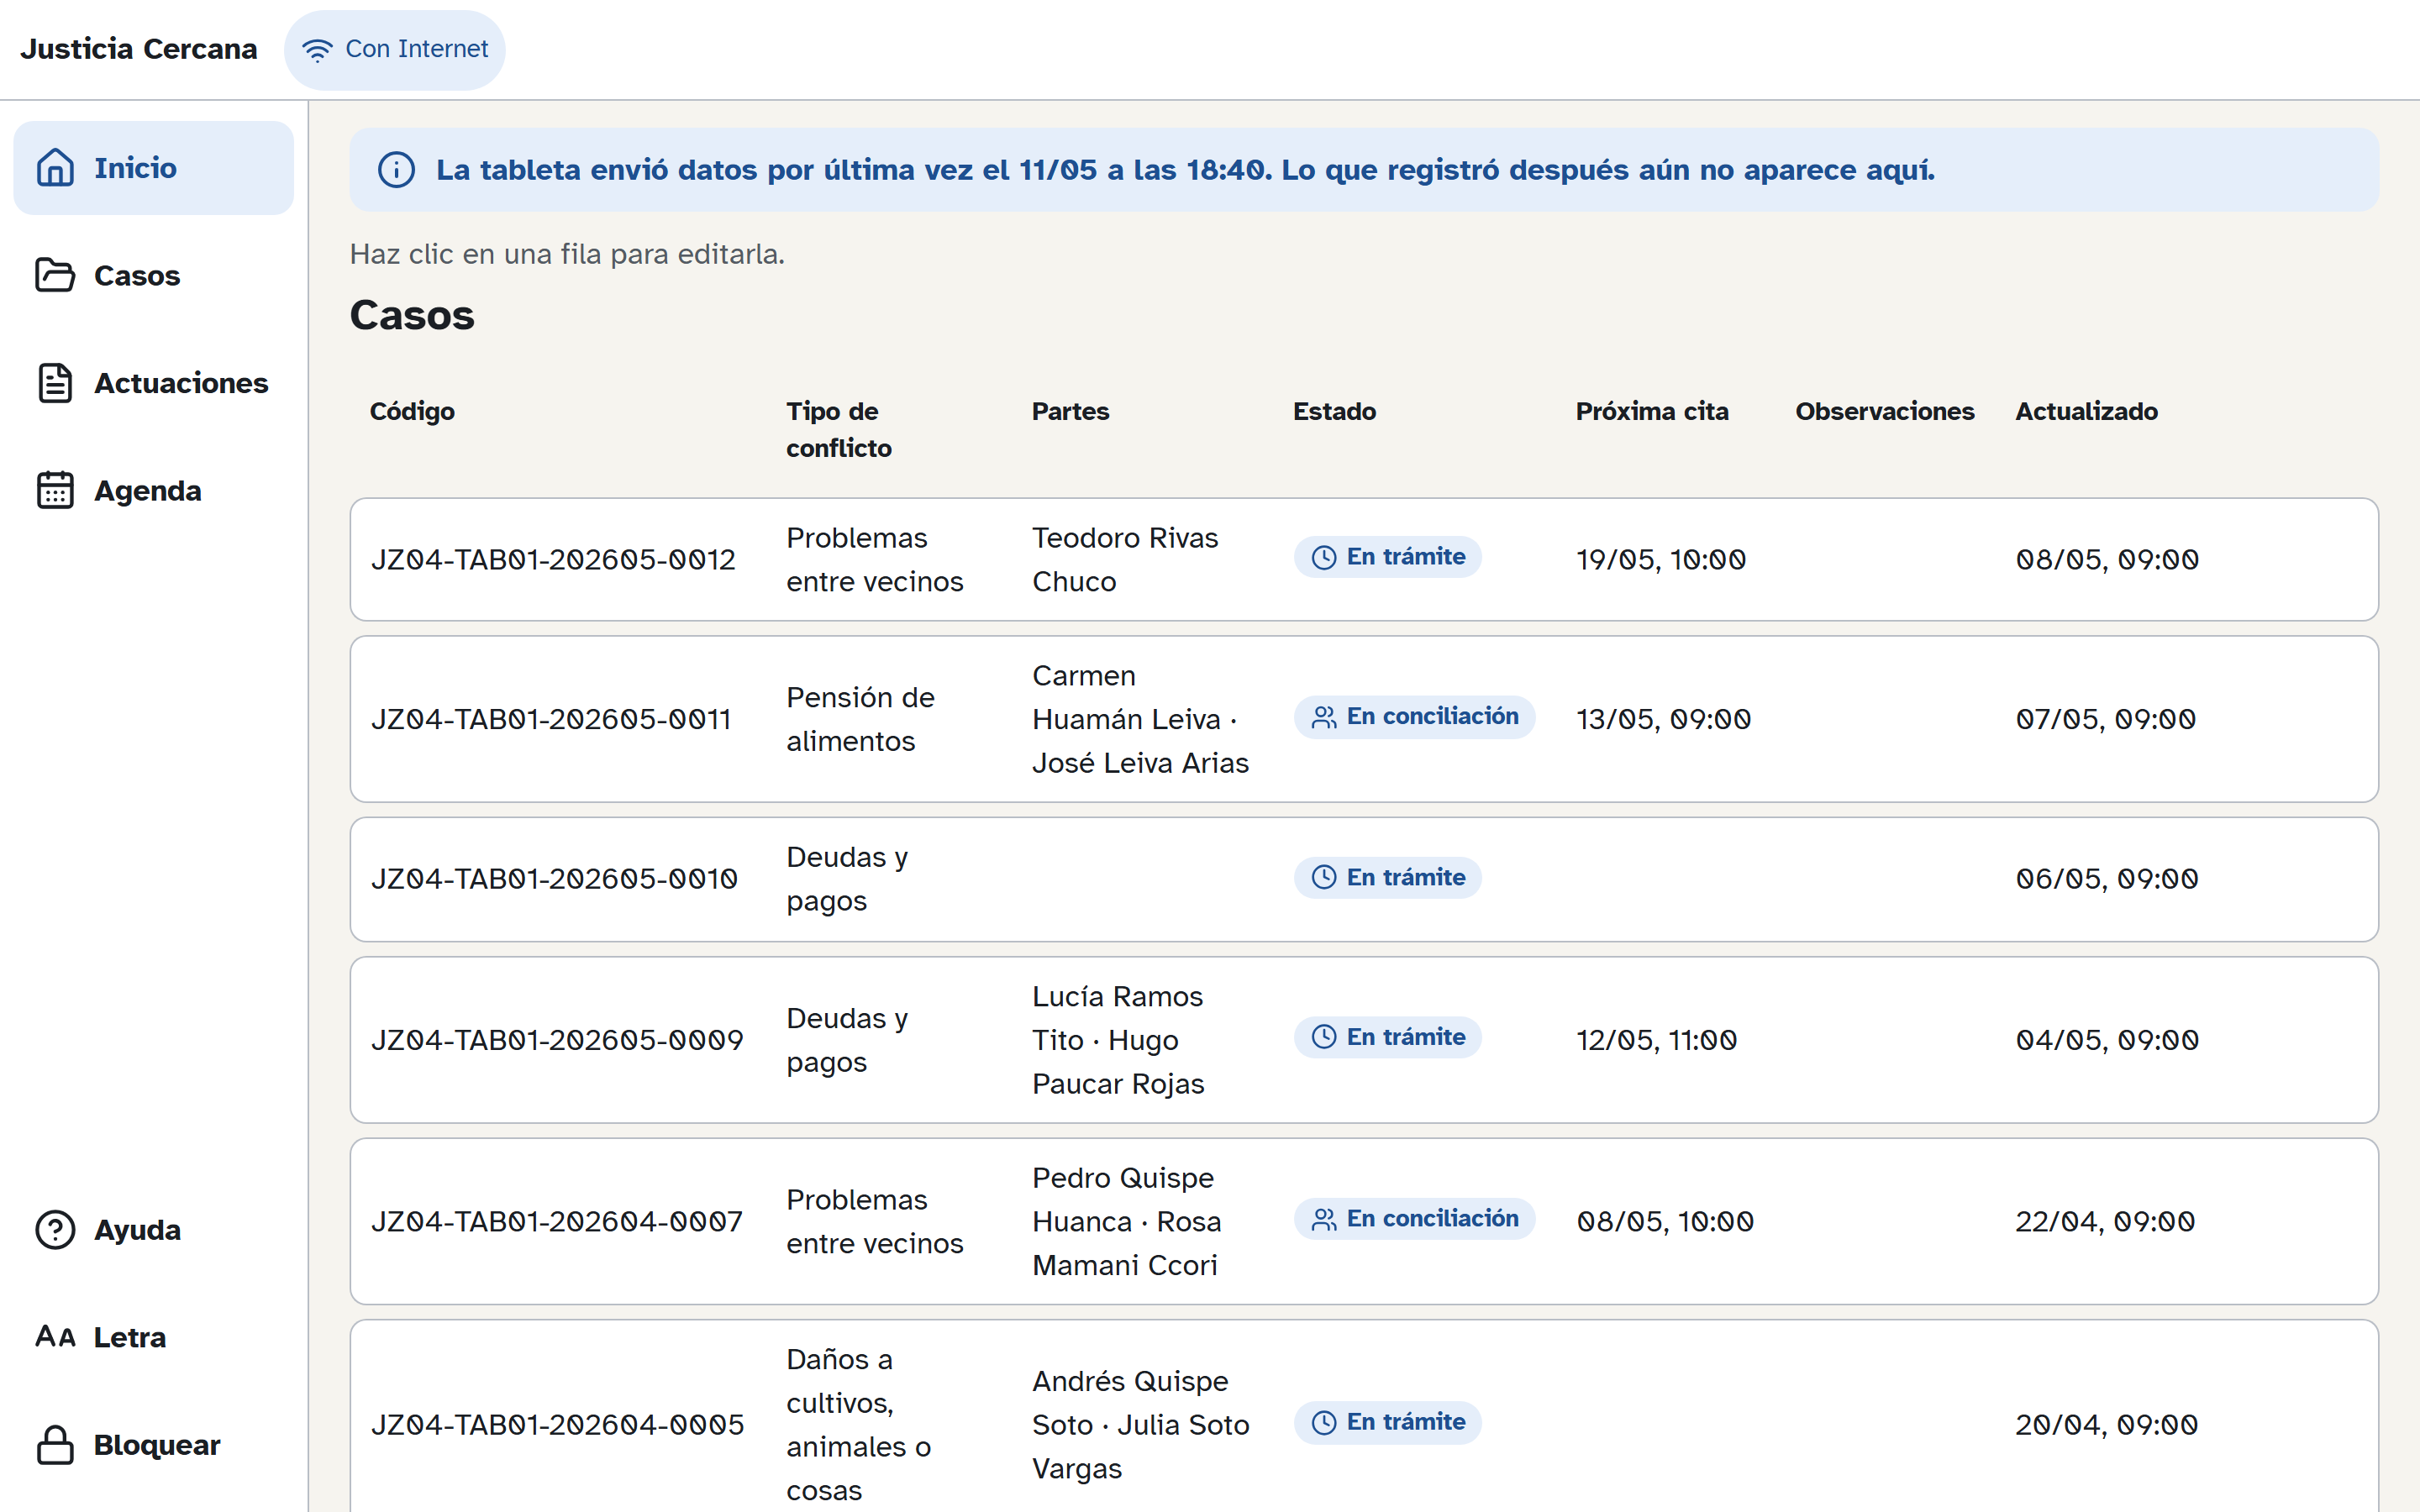
\includegraphics[width=\linewidth]{../../captures/FB-01_computadora-aviso.png}\\[-2pt]{\footnotesize\raggedright\textbf{P-10 · 1.} Vista en computadora 1440×900 con aviso del último envío; no afirma pendientes de la tableta \emph{(Funcionamiento sin conexión)}\par}\end{minipage}\hfill
\begin{minipage}[t]{0.49\textwidth}\centering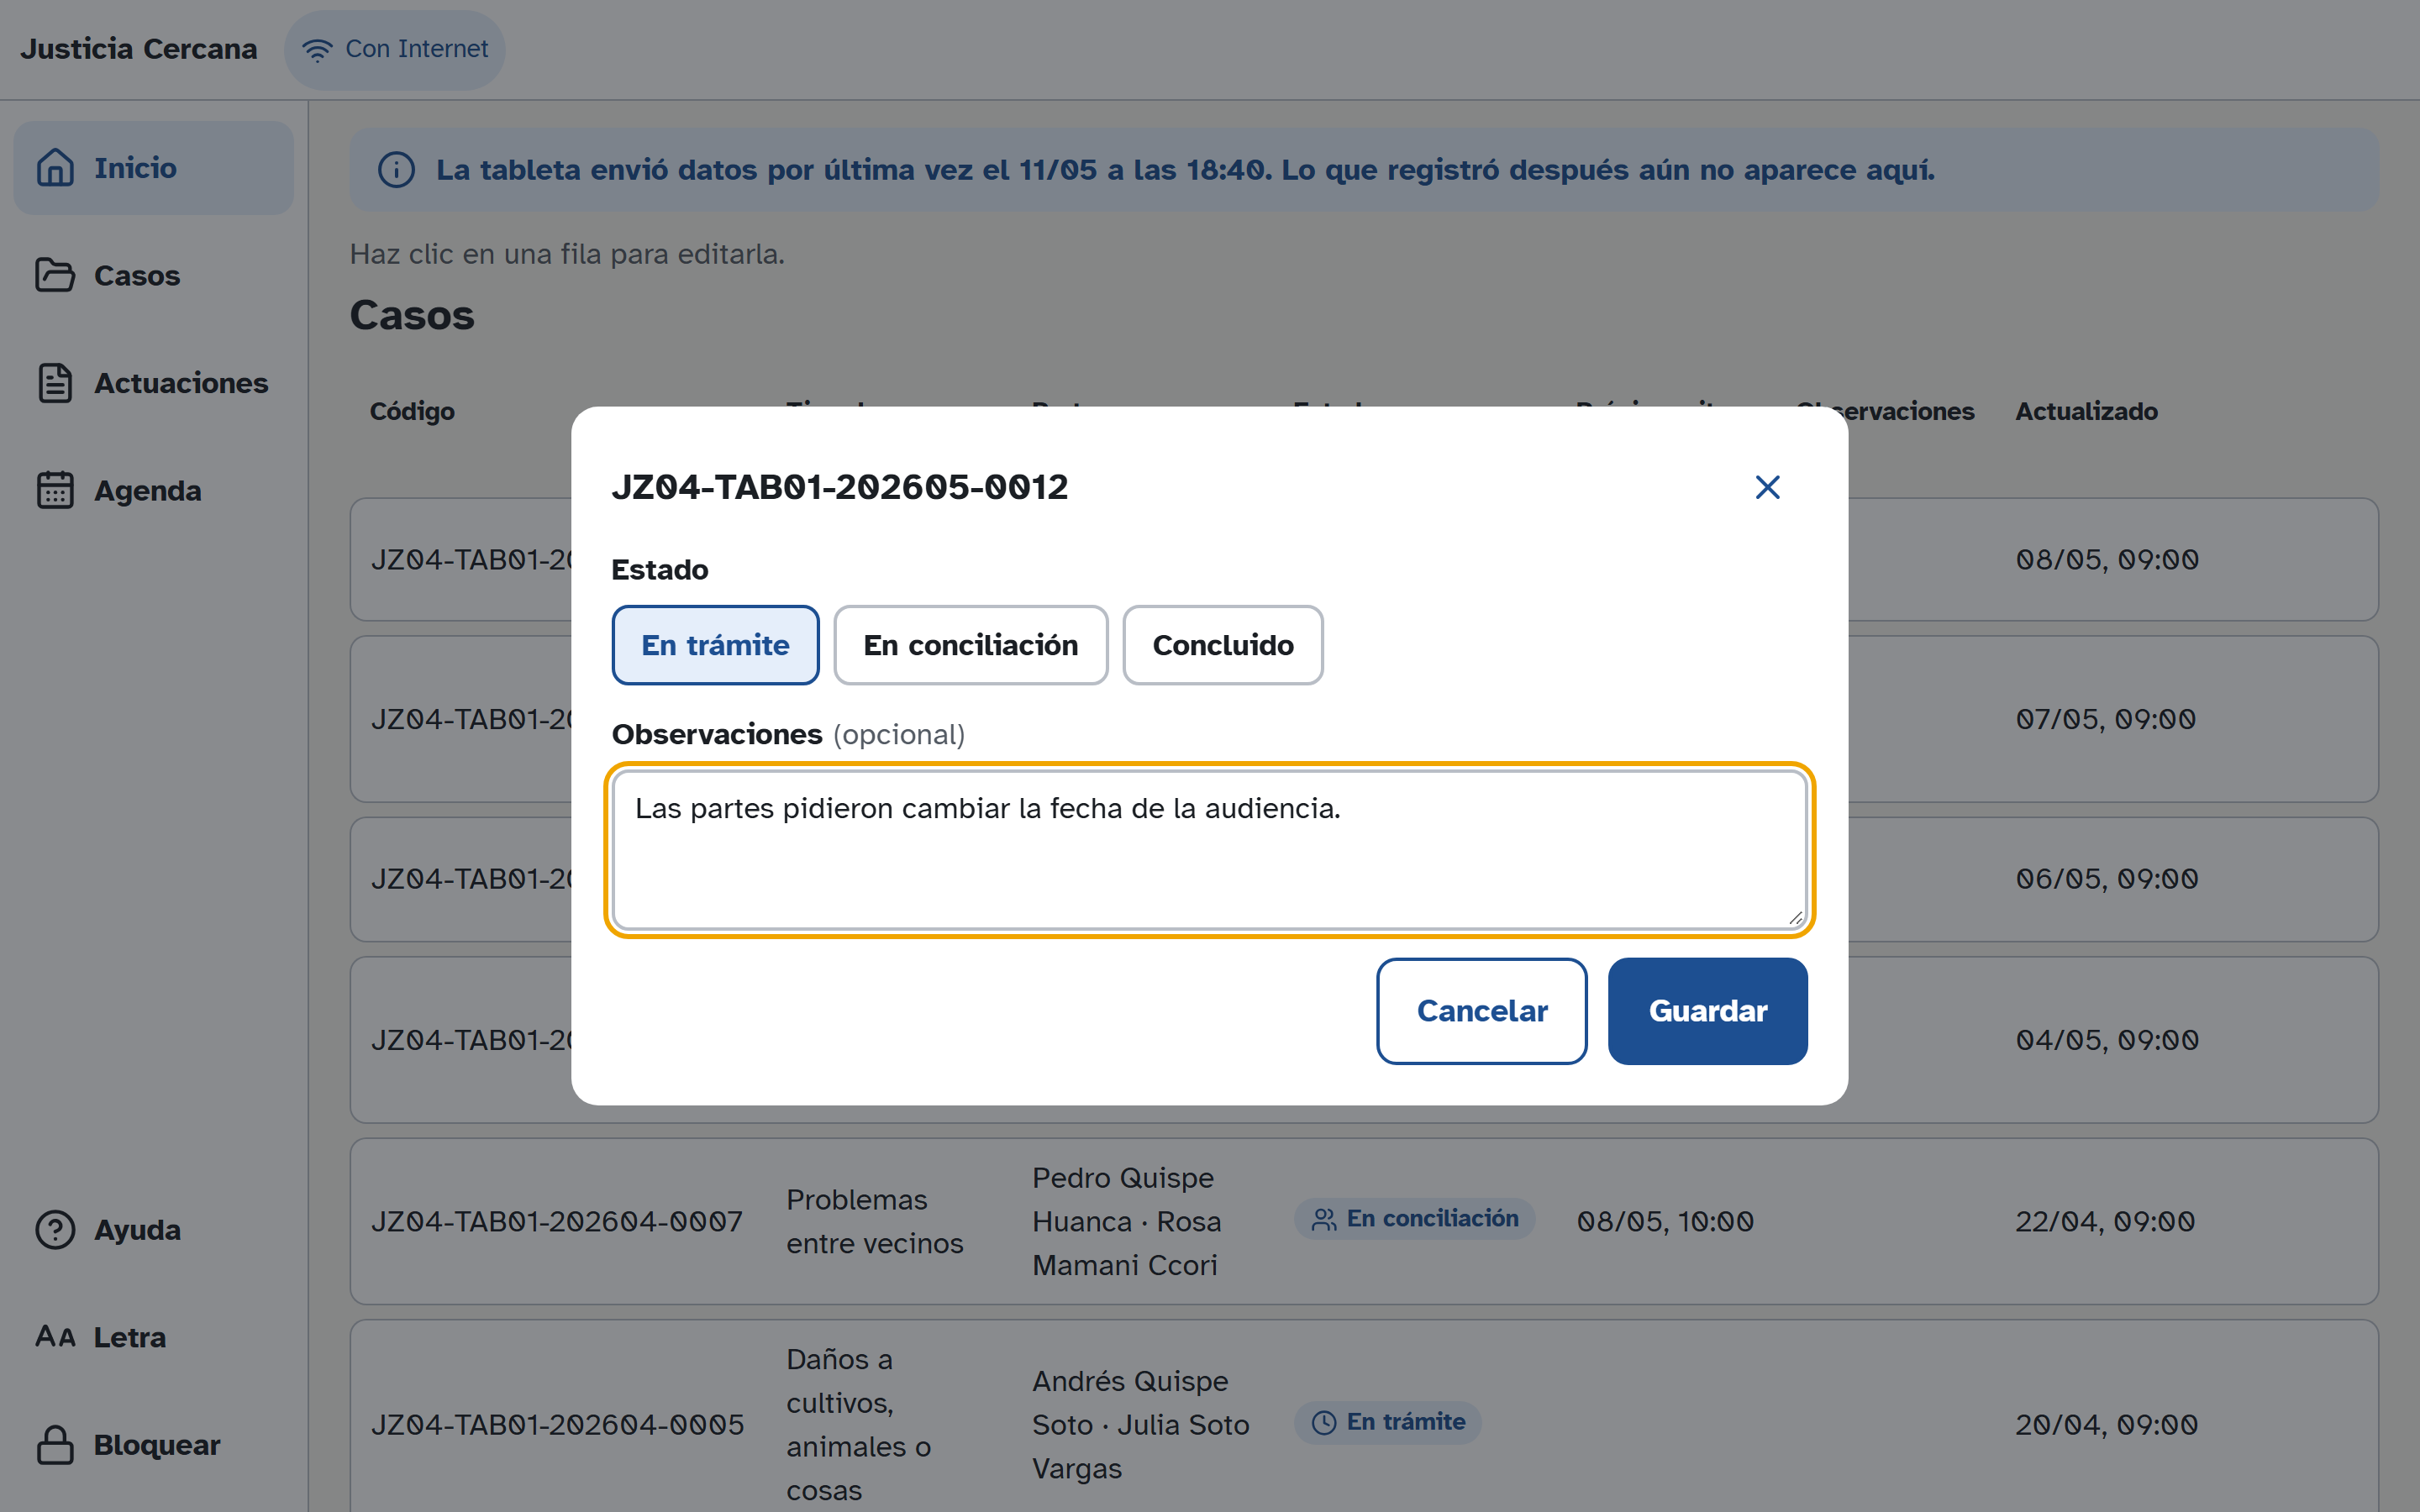
\includegraphics[width=\linewidth]{../../captures/FB-02_editar-caso.png}\\[-2pt]{\footnotesize\raggedright\textbf{P-10 · 2.} Edición de un caso desde la computadora (origen de conflicto) \emph{(Cobertura y funcionamiento de los módulos)}\par}\end{minipage}\par\vspace{8pt}\noindent
\begin{minipage}[t]{0.49\textwidth}\centering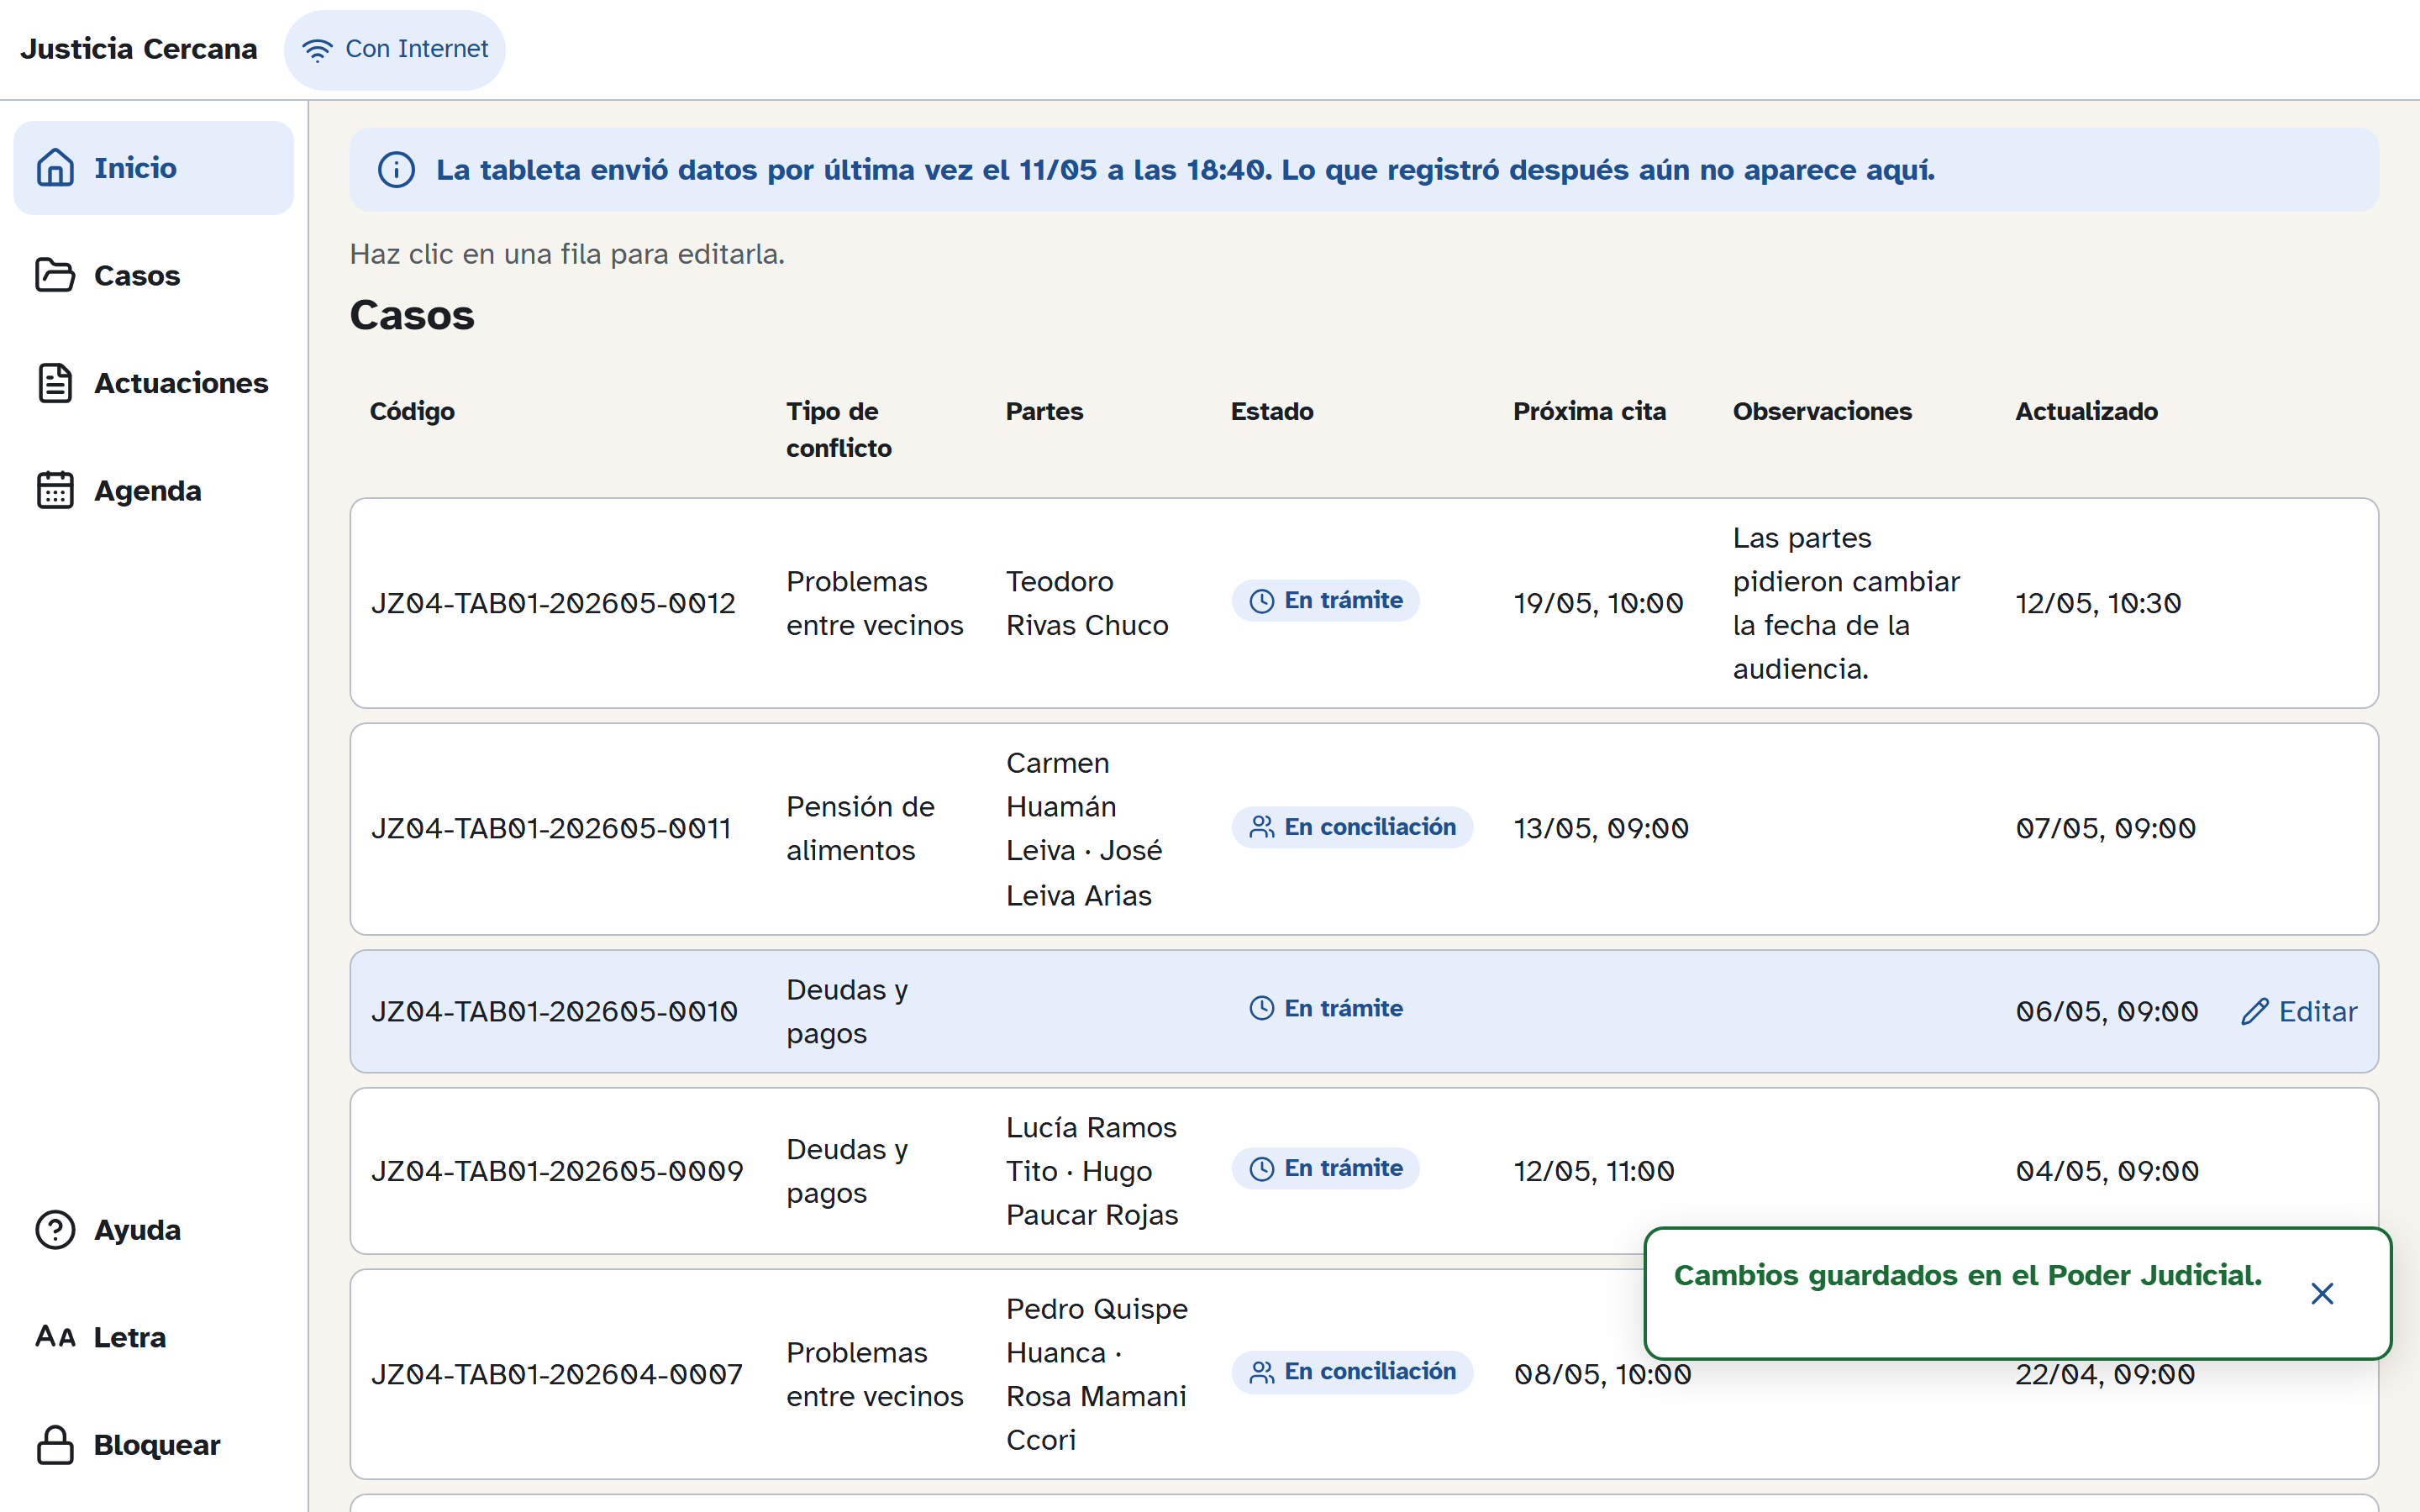
\includegraphics[width=\linewidth]{../../captures/FB-03_guardado-computadora.png}\\[-2pt]{\footnotesize\raggedright\textbf{P-10 · 2.} Cambio guardado en el Poder Judicial \emph{(Cobertura y funcionamiento de los módulos)}\par}\end{minipage}\hfill
\par\vspace{4pt}
